\documentclass[letterpaper,12pt]{article}
\usepackage[english]{babel}
\usepackage[utf8x]{inputenc}
\usepackage[T1]{fontenc}
\usepackage{titlesec}
\usepackage[letterpaper,top=1in,bottom=1in,left=1in,right=1in,marginparwidth=0in]{geometry}
\usepackage{times}
\usepackage{amsmath}
\usepackage{graphicx}
\usepackage[colorlinks=true, allcolors=blue]{hyperref}
\usepackage{enumitem} 
\usepackage{natbib} 
\usepackage{libertine}
\usepackage{float}
\begin{document}
\fontfamily{ptm}\selectfont
\urlstyle{same}
\urlstyle{rm}
\tableofcontents
\pagebreak




% Time series for each predictor variable 

\subsection{ML Inputs (with NAs) Time Series Images} 
 

\begin{figure} 
\centering  
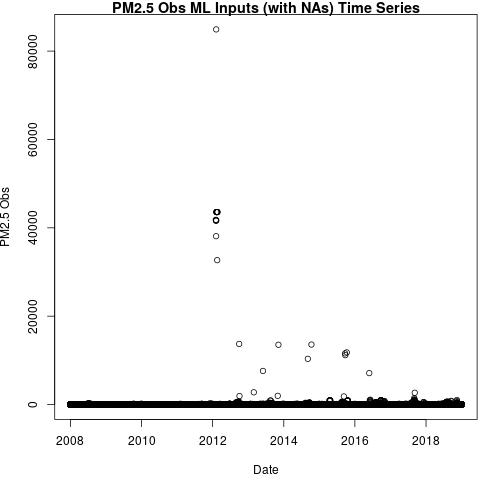
\includegraphics[width=0.77\textwidth]{Code_Outputs/Report_ML_input_PM25_Step4_part_f_de_duplicated_aves_prioritize_24hr_obswNAs_PM25_ObsvDate.jpg} 
\caption{\label{fig:Report_ML_input_PM25_Step4_part_f_de_duplicated_aves_prioritize_24hr_obswNAsPM25_ObsvDate}ML Inputs (with NAs) Time Series} 
\end{figure} 
 

\begin{figure} 
\centering  
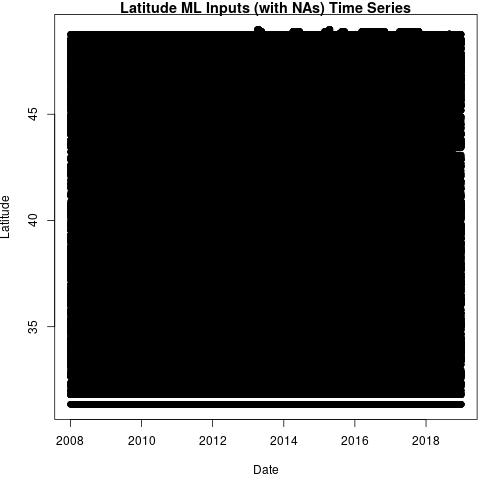
\includegraphics[width=0.77\textwidth]{Code_Outputs/Report_ML_input_PM25_Step4_part_f_de_duplicated_aves_prioritize_24hr_obswNAs_LatitudevDate.jpg} 
\caption{\label{fig:Report_ML_input_PM25_Step4_part_f_de_duplicated_aves_prioritize_24hr_obswNAsLatitudevDate}ML Inputs (with NAs) Time Series} 
\end{figure} 
 

\begin{figure} 
\centering  
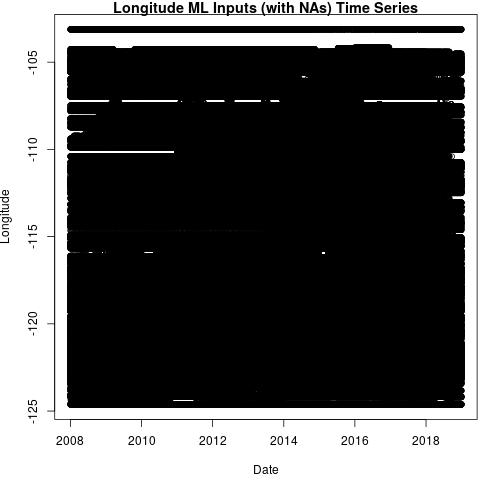
\includegraphics[width=0.77\textwidth]{Code_Outputs/Report_ML_input_PM25_Step4_part_f_de_duplicated_aves_prioritize_24hr_obswNAs_LongitudevDate.jpg} 
\caption{\label{fig:Report_ML_input_PM25_Step4_part_f_de_duplicated_aves_prioritize_24hr_obswNAsLongitudevDate}ML Inputs (with NAs) Time Series} 
\end{figure} 
 

\begin{figure} 
\centering  
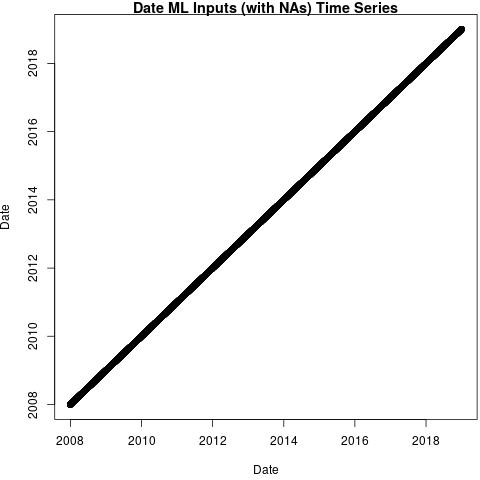
\includegraphics[width=0.77\textwidth]{Code_Outputs/Report_ML_input_PM25_Step4_part_f_de_duplicated_aves_prioritize_24hr_obswNAs_DatevDate.jpg} 
\caption{\label{fig:Report_ML_input_PM25_Step4_part_f_de_duplicated_aves_prioritize_24hr_obswNAsDatevDate}ML Inputs (with NAs) Time Series} 
\end{figure} 
 

\begin{figure} 
\centering  
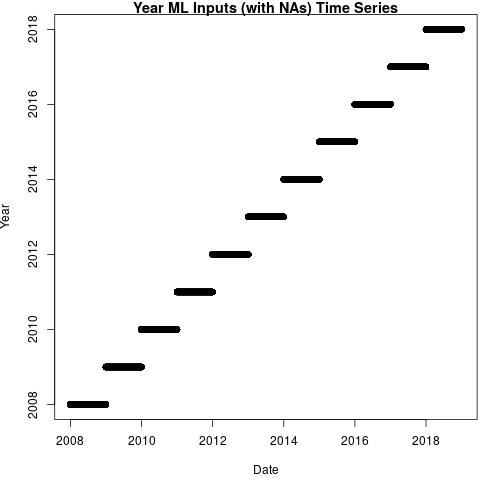
\includegraphics[width=0.77\textwidth]{Code_Outputs/Report_ML_input_PM25_Step4_part_f_de_duplicated_aves_prioritize_24hr_obswNAs_YearvDate.jpg} 
\caption{\label{fig:Report_ML_input_PM25_Step4_part_f_de_duplicated_aves_prioritize_24hr_obswNAsYearvDate}ML Inputs (with NAs) Time Series} 
\end{figure} 
 

\begin{figure} 
\centering  
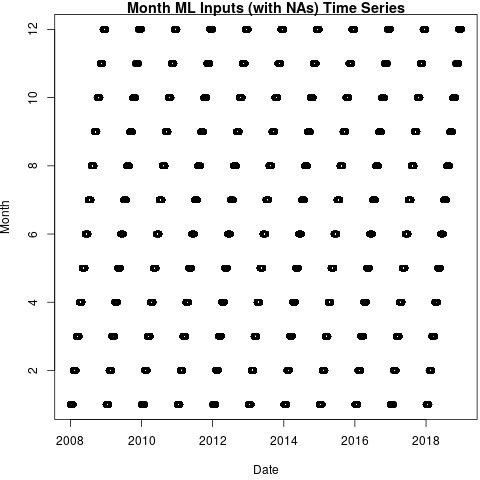
\includegraphics[width=0.77\textwidth]{Code_Outputs/Report_ML_input_PM25_Step4_part_f_de_duplicated_aves_prioritize_24hr_obswNAs_MonthvDate.jpg} 
\caption{\label{fig:Report_ML_input_PM25_Step4_part_f_de_duplicated_aves_prioritize_24hr_obswNAsMonthvDate}ML Inputs (with NAs) Time Series} 
\end{figure} 
 

\begin{figure} 
\centering  
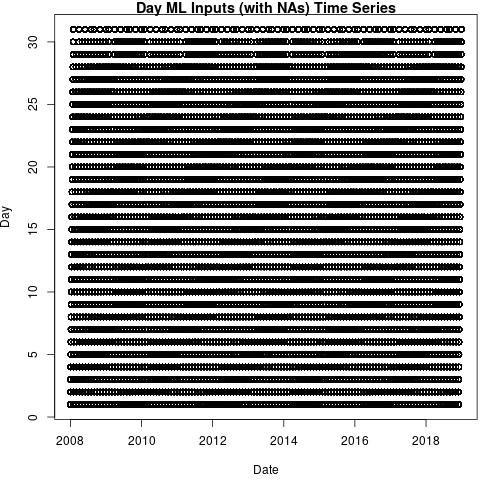
\includegraphics[width=0.77\textwidth]{Code_Outputs/Report_ML_input_PM25_Step4_part_f_de_duplicated_aves_prioritize_24hr_obswNAs_DayvDate.jpg} 
\caption{\label{fig:Report_ML_input_PM25_Step4_part_f_de_duplicated_aves_prioritize_24hr_obswNAsDayvDate}ML Inputs (with NAs) Time Series} 
\end{figure} 
 

\begin{figure} 
\centering  
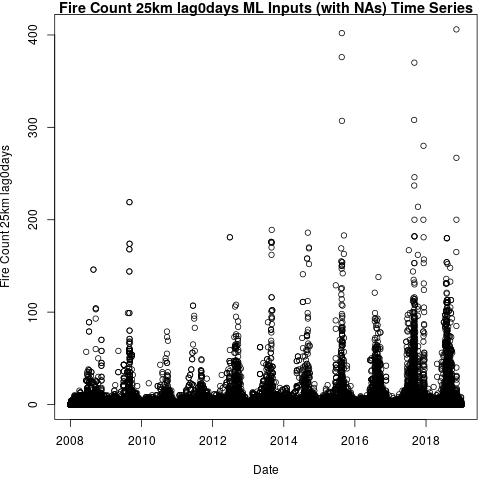
\includegraphics[width=0.77\textwidth]{Code_Outputs/Report_ML_input_PM25_Step4_part_f_de_duplicated_aves_prioritize_24hr_obswNAs_Fire_Count_25km_lag0daysvDate.jpg} 
\caption{\label{fig:Report_ML_input_PM25_Step4_part_f_de_duplicated_aves_prioritize_24hr_obswNAsFire_Count_25km_lag0daysvDate}ML Inputs (with NAs) Time Series} 
\end{figure} 
 

\begin{figure} 
\centering  
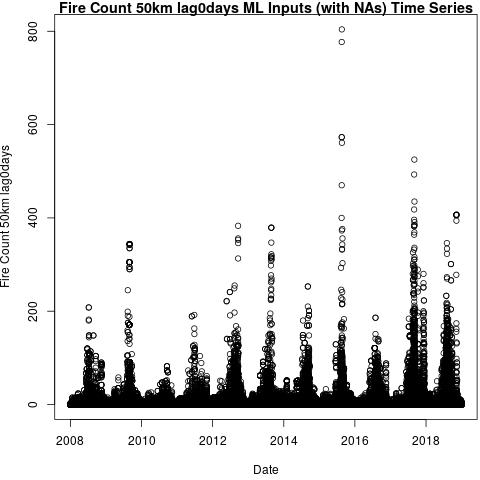
\includegraphics[width=0.77\textwidth]{Code_Outputs/Report_ML_input_PM25_Step4_part_f_de_duplicated_aves_prioritize_24hr_obswNAs_Fire_Count_50km_lag0daysvDate.jpg} 
\caption{\label{fig:Report_ML_input_PM25_Step4_part_f_de_duplicated_aves_prioritize_24hr_obswNAsFire_Count_50km_lag0daysvDate}ML Inputs (with NAs) Time Series} 
\end{figure} 
 

\clearpage 

\begin{figure} 
\centering  
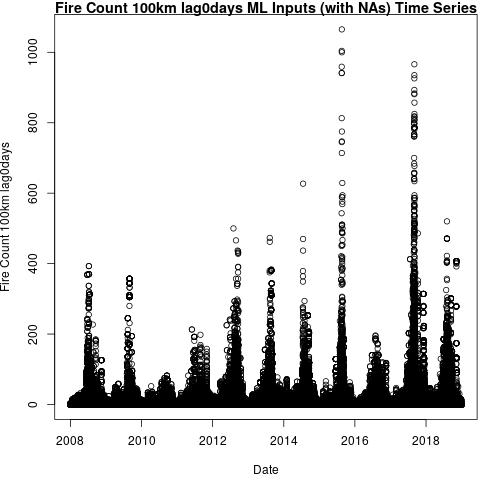
\includegraphics[width=0.77\textwidth]{Code_Outputs/Report_ML_input_PM25_Step4_part_f_de_duplicated_aves_prioritize_24hr_obswNAs_Fire_Count_100km_lag0daysvDate.jpg} 
\caption{\label{fig:Report_ML_input_PM25_Step4_part_f_de_duplicated_aves_prioritize_24hr_obswNAsFire_Count_100km_lag0daysvDate}ML Inputs (with NAs) Time Series} 
\end{figure} 
 

\begin{figure} 
\centering  
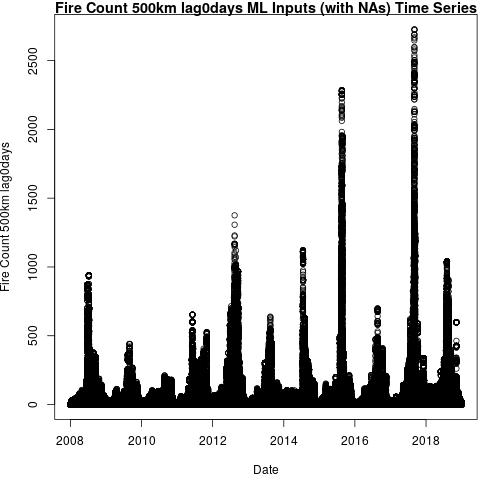
\includegraphics[width=0.77\textwidth]{Code_Outputs/Report_ML_input_PM25_Step4_part_f_de_duplicated_aves_prioritize_24hr_obswNAs_Fire_Count_500km_lag0daysvDate.jpg} 
\caption{\label{fig:Report_ML_input_PM25_Step4_part_f_de_duplicated_aves_prioritize_24hr_obswNAsFire_Count_500km_lag0daysvDate}ML Inputs (with NAs) Time Series} 
\end{figure} 
 

\begin{figure} 
\centering  
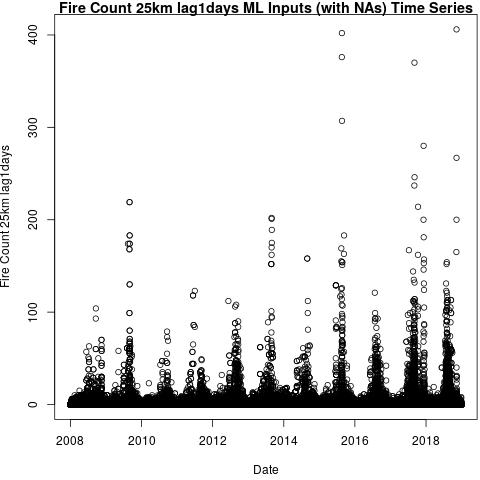
\includegraphics[width=0.77\textwidth]{Code_Outputs/Report_ML_input_PM25_Step4_part_f_de_duplicated_aves_prioritize_24hr_obswNAs_Fire_Count_25km_lag1daysvDate.jpg} 
\caption{\label{fig:Report_ML_input_PM25_Step4_part_f_de_duplicated_aves_prioritize_24hr_obswNAsFire_Count_25km_lag1daysvDate}ML Inputs (with NAs) Time Series} 
\end{figure} 
 

\begin{figure} 
\centering  
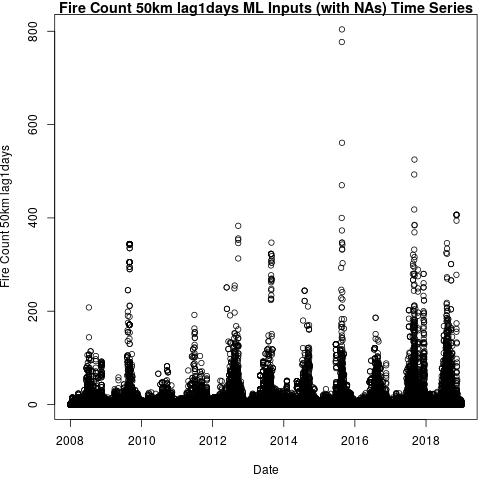
\includegraphics[width=0.77\textwidth]{Code_Outputs/Report_ML_input_PM25_Step4_part_f_de_duplicated_aves_prioritize_24hr_obswNAs_Fire_Count_50km_lag1daysvDate.jpg} 
\caption{\label{fig:Report_ML_input_PM25_Step4_part_f_de_duplicated_aves_prioritize_24hr_obswNAsFire_Count_50km_lag1daysvDate}ML Inputs (with NAs) Time Series} 
\end{figure} 
 

\begin{figure} 
\centering  
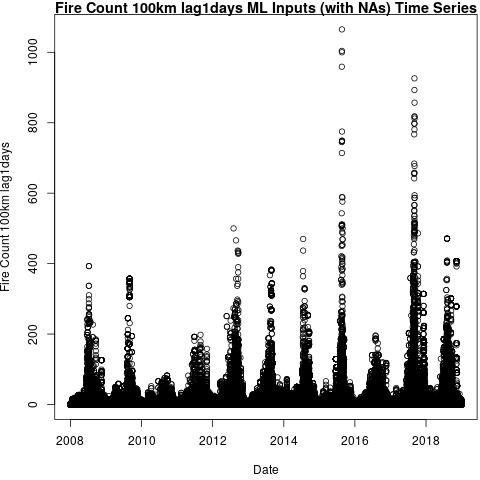
\includegraphics[width=0.77\textwidth]{Code_Outputs/Report_ML_input_PM25_Step4_part_f_de_duplicated_aves_prioritize_24hr_obswNAs_Fire_Count_100km_lag1daysvDate.jpg} 
\caption{\label{fig:Report_ML_input_PM25_Step4_part_f_de_duplicated_aves_prioritize_24hr_obswNAsFire_Count_100km_lag1daysvDate}ML Inputs (with NAs) Time Series} 
\end{figure} 
 

\begin{figure} 
\centering  
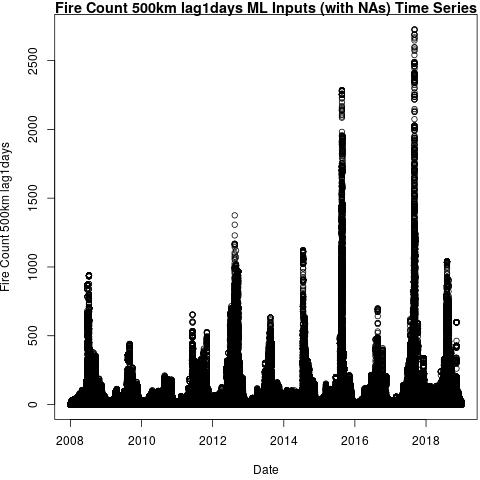
\includegraphics[width=0.77\textwidth]{Code_Outputs/Report_ML_input_PM25_Step4_part_f_de_duplicated_aves_prioritize_24hr_obswNAs_Fire_Count_500km_lag1daysvDate.jpg} 
\caption{\label{fig:Report_ML_input_PM25_Step4_part_f_de_duplicated_aves_prioritize_24hr_obswNAsFire_Count_500km_lag1daysvDate}ML Inputs (with NAs) Time Series} 
\end{figure} 
 

\begin{figure} 
\centering  
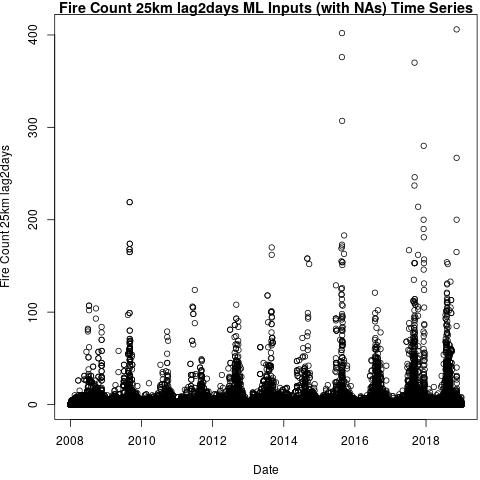
\includegraphics[width=0.77\textwidth]{Code_Outputs/Report_ML_input_PM25_Step4_part_f_de_duplicated_aves_prioritize_24hr_obswNAs_Fire_Count_25km_lag2daysvDate.jpg} 
\caption{\label{fig:Report_ML_input_PM25_Step4_part_f_de_duplicated_aves_prioritize_24hr_obswNAsFire_Count_25km_lag2daysvDate}ML Inputs (with NAs) Time Series} 
\end{figure} 
 

\begin{figure} 
\centering  
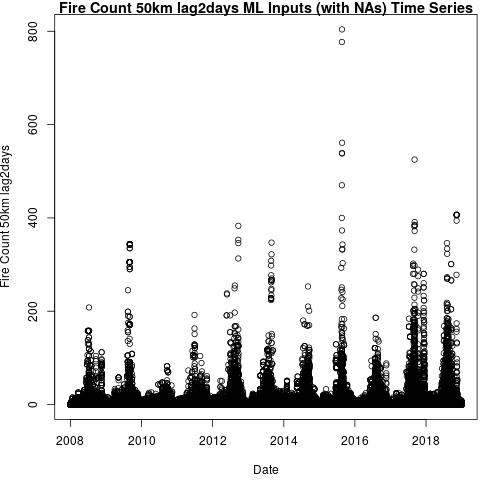
\includegraphics[width=0.77\textwidth]{Code_Outputs/Report_ML_input_PM25_Step4_part_f_de_duplicated_aves_prioritize_24hr_obswNAs_Fire_Count_50km_lag2daysvDate.jpg} 
\caption{\label{fig:Report_ML_input_PM25_Step4_part_f_de_duplicated_aves_prioritize_24hr_obswNAsFire_Count_50km_lag2daysvDate}ML Inputs (with NAs) Time Series} 
\end{figure} 
 

\begin{figure} 
\centering  
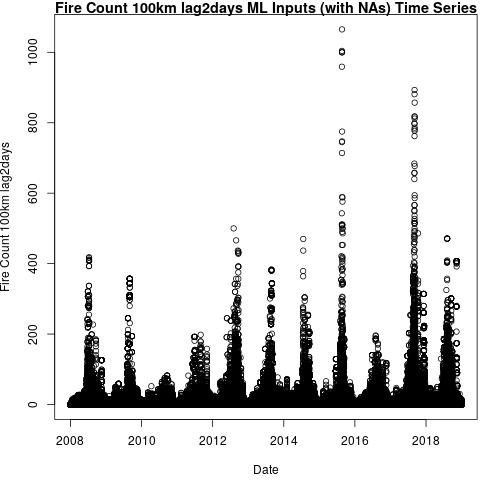
\includegraphics[width=0.77\textwidth]{Code_Outputs/Report_ML_input_PM25_Step4_part_f_de_duplicated_aves_prioritize_24hr_obswNAs_Fire_Count_100km_lag2daysvDate.jpg} 
\caption{\label{fig:Report_ML_input_PM25_Step4_part_f_de_duplicated_aves_prioritize_24hr_obswNAsFire_Count_100km_lag2daysvDate}ML Inputs (with NAs) Time Series} 
\end{figure} 
 

\begin{figure} 
\centering  
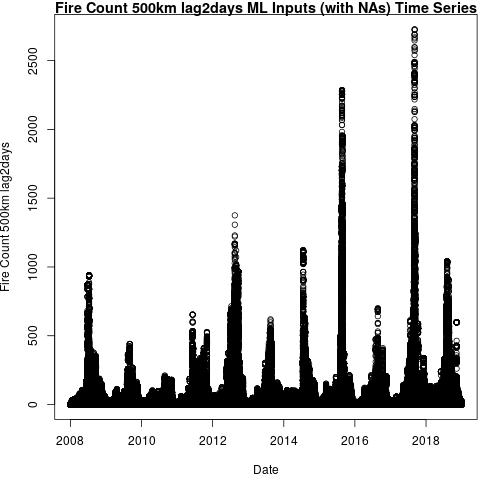
\includegraphics[width=0.77\textwidth]{Code_Outputs/Report_ML_input_PM25_Step4_part_f_de_duplicated_aves_prioritize_24hr_obswNAs_Fire_Count_500km_lag2daysvDate.jpg} 
\caption{\label{fig:Report_ML_input_PM25_Step4_part_f_de_duplicated_aves_prioritize_24hr_obswNAsFire_Count_500km_lag2daysvDate}ML Inputs (with NAs) Time Series} 
\end{figure} 
 

\clearpage 

\begin{figure} 
\centering  
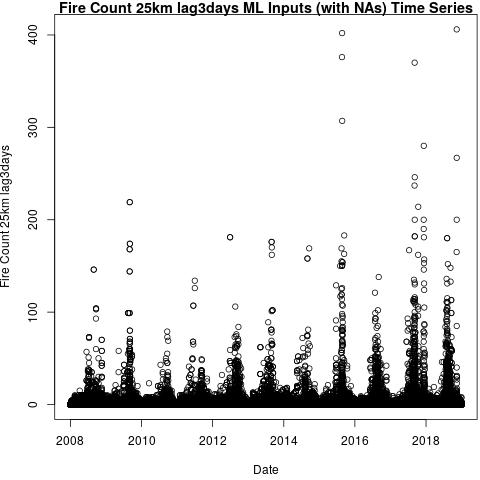
\includegraphics[width=0.77\textwidth]{Code_Outputs/Report_ML_input_PM25_Step4_part_f_de_duplicated_aves_prioritize_24hr_obswNAs_Fire_Count_25km_lag3daysvDate.jpg} 
\caption{\label{fig:Report_ML_input_PM25_Step4_part_f_de_duplicated_aves_prioritize_24hr_obswNAsFire_Count_25km_lag3daysvDate}ML Inputs (with NAs) Time Series} 
\end{figure} 
 

\begin{figure} 
\centering  
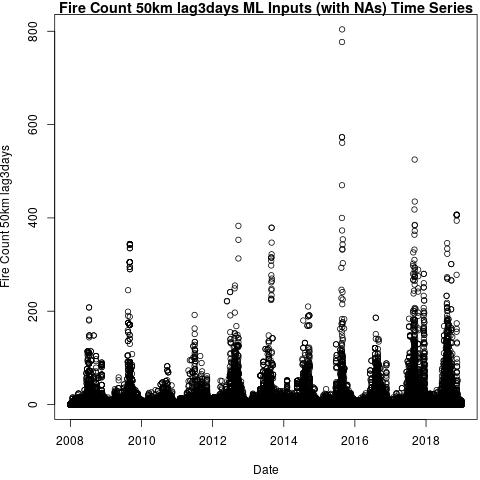
\includegraphics[width=0.77\textwidth]{Code_Outputs/Report_ML_input_PM25_Step4_part_f_de_duplicated_aves_prioritize_24hr_obswNAs_Fire_Count_50km_lag3daysvDate.jpg} 
\caption{\label{fig:Report_ML_input_PM25_Step4_part_f_de_duplicated_aves_prioritize_24hr_obswNAsFire_Count_50km_lag3daysvDate}ML Inputs (with NAs) Time Series} 
\end{figure} 
 

\begin{figure} 
\centering  
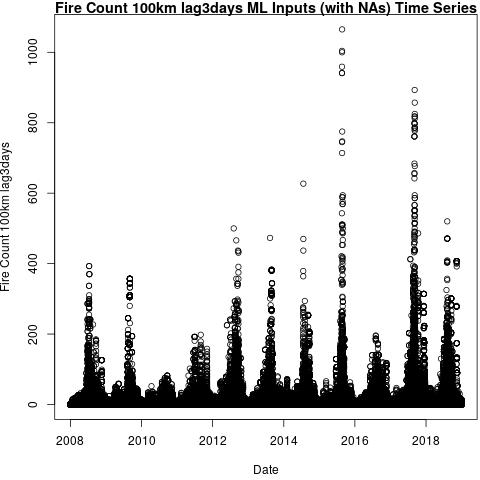
\includegraphics[width=0.77\textwidth]{Code_Outputs/Report_ML_input_PM25_Step4_part_f_de_duplicated_aves_prioritize_24hr_obswNAs_Fire_Count_100km_lag3daysvDate.jpg} 
\caption{\label{fig:Report_ML_input_PM25_Step4_part_f_de_duplicated_aves_prioritize_24hr_obswNAsFire_Count_100km_lag3daysvDate}ML Inputs (with NAs) Time Series} 
\end{figure} 
 

\begin{figure} 
\centering  
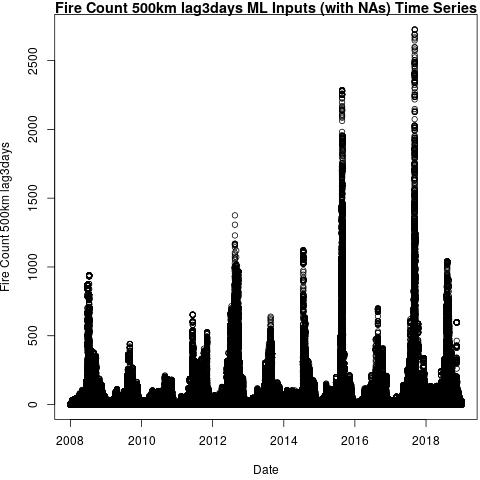
\includegraphics[width=0.77\textwidth]{Code_Outputs/Report_ML_input_PM25_Step4_part_f_de_duplicated_aves_prioritize_24hr_obswNAs_Fire_Count_500km_lag3daysvDate.jpg} 
\caption{\label{fig:Report_ML_input_PM25_Step4_part_f_de_duplicated_aves_prioritize_24hr_obswNAsFire_Count_500km_lag3daysvDate}ML Inputs (with NAs) Time Series} 
\end{figure} 
 

\begin{figure} 
\centering  
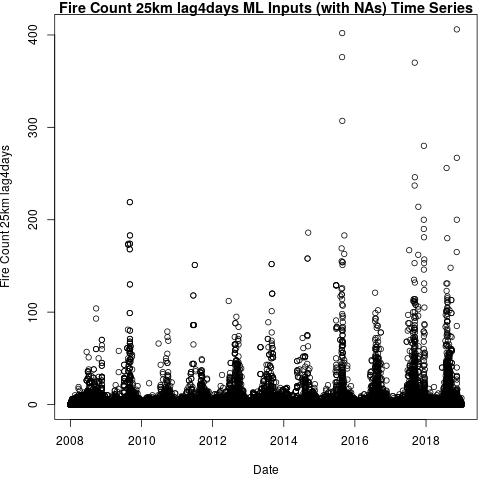
\includegraphics[width=0.77\textwidth]{Code_Outputs/Report_ML_input_PM25_Step4_part_f_de_duplicated_aves_prioritize_24hr_obswNAs_Fire_Count_25km_lag4daysvDate.jpg} 
\caption{\label{fig:Report_ML_input_PM25_Step4_part_f_de_duplicated_aves_prioritize_24hr_obswNAsFire_Count_25km_lag4daysvDate}ML Inputs (with NAs) Time Series} 
\end{figure} 
 

\begin{figure} 
\centering  
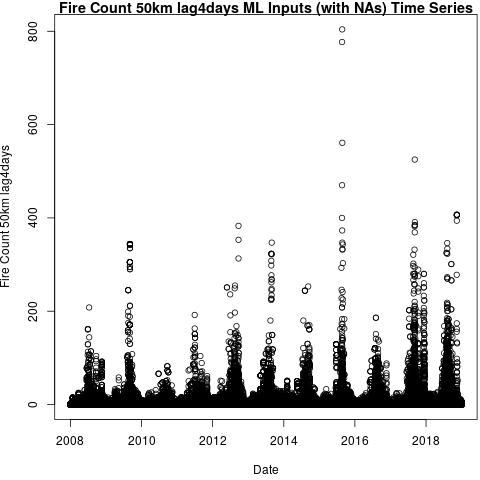
\includegraphics[width=0.77\textwidth]{Code_Outputs/Report_ML_input_PM25_Step4_part_f_de_duplicated_aves_prioritize_24hr_obswNAs_Fire_Count_50km_lag4daysvDate.jpg} 
\caption{\label{fig:Report_ML_input_PM25_Step4_part_f_de_duplicated_aves_prioritize_24hr_obswNAsFire_Count_50km_lag4daysvDate}ML Inputs (with NAs) Time Series} 
\end{figure} 
 

\begin{figure} 
\centering  
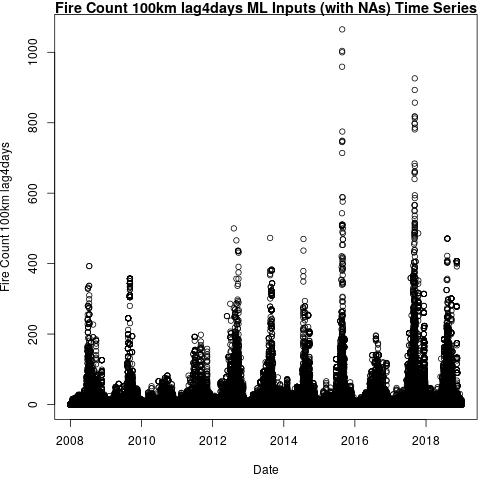
\includegraphics[width=0.77\textwidth]{Code_Outputs/Report_ML_input_PM25_Step4_part_f_de_duplicated_aves_prioritize_24hr_obswNAs_Fire_Count_100km_lag4daysvDate.jpg} 
\caption{\label{fig:Report_ML_input_PM25_Step4_part_f_de_duplicated_aves_prioritize_24hr_obswNAsFire_Count_100km_lag4daysvDate}ML Inputs (with NAs) Time Series} 
\end{figure} 
 

\begin{figure} 
\centering  
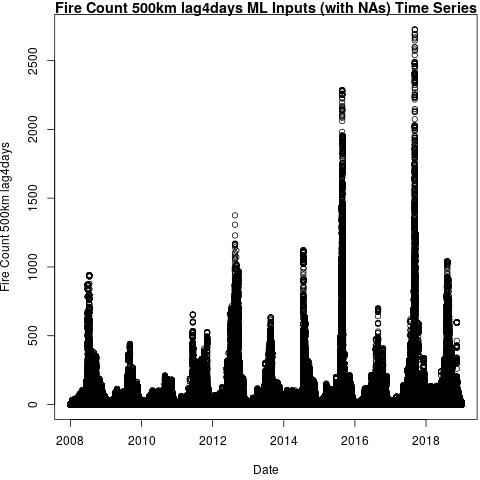
\includegraphics[width=0.77\textwidth]{Code_Outputs/Report_ML_input_PM25_Step4_part_f_de_duplicated_aves_prioritize_24hr_obswNAs_Fire_Count_500km_lag4daysvDate.jpg} 
\caption{\label{fig:Report_ML_input_PM25_Step4_part_f_de_duplicated_aves_prioritize_24hr_obswNAsFire_Count_500km_lag4daysvDate}ML Inputs (with NAs) Time Series} 
\end{figure} 
 

\begin{figure} 
\centering  
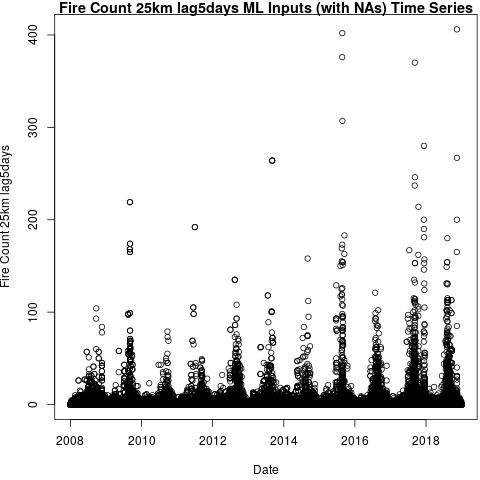
\includegraphics[width=0.77\textwidth]{Code_Outputs/Report_ML_input_PM25_Step4_part_f_de_duplicated_aves_prioritize_24hr_obswNAs_Fire_Count_25km_lag5daysvDate.jpg} 
\caption{\label{fig:Report_ML_input_PM25_Step4_part_f_de_duplicated_aves_prioritize_24hr_obswNAsFire_Count_25km_lag5daysvDate}ML Inputs (with NAs) Time Series} 
\end{figure} 
 

\begin{figure} 
\centering  
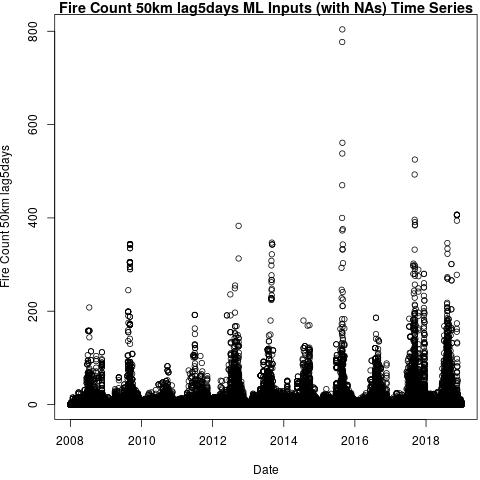
\includegraphics[width=0.77\textwidth]{Code_Outputs/Report_ML_input_PM25_Step4_part_f_de_duplicated_aves_prioritize_24hr_obswNAs_Fire_Count_50km_lag5daysvDate.jpg} 
\caption{\label{fig:Report_ML_input_PM25_Step4_part_f_de_duplicated_aves_prioritize_24hr_obswNAsFire_Count_50km_lag5daysvDate}ML Inputs (with NAs) Time Series} 
\end{figure} 
 

\clearpage 

\begin{figure} 
\centering  
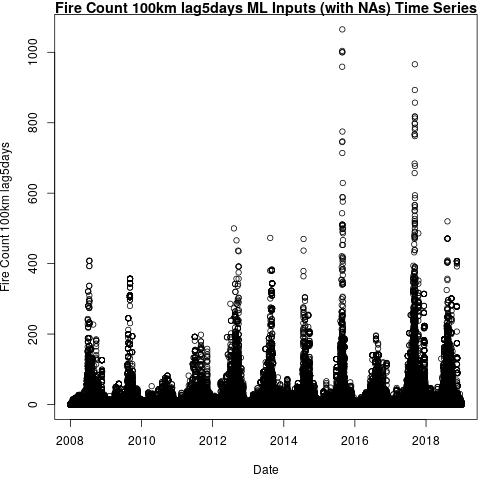
\includegraphics[width=0.77\textwidth]{Code_Outputs/Report_ML_input_PM25_Step4_part_f_de_duplicated_aves_prioritize_24hr_obswNAs_Fire_Count_100km_lag5daysvDate.jpg} 
\caption{\label{fig:Report_ML_input_PM25_Step4_part_f_de_duplicated_aves_prioritize_24hr_obswNAsFire_Count_100km_lag5daysvDate}ML Inputs (with NAs) Time Series} 
\end{figure} 
 

\begin{figure} 
\centering  
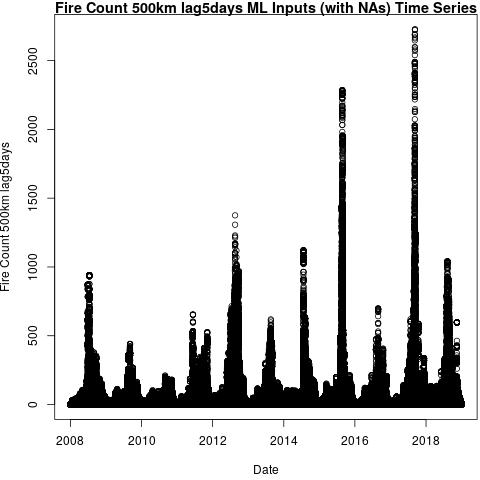
\includegraphics[width=0.77\textwidth]{Code_Outputs/Report_ML_input_PM25_Step4_part_f_de_duplicated_aves_prioritize_24hr_obswNAs_Fire_Count_500km_lag5daysvDate.jpg} 
\caption{\label{fig:Report_ML_input_PM25_Step4_part_f_de_duplicated_aves_prioritize_24hr_obswNAsFire_Count_500km_lag5daysvDate}ML Inputs (with NAs) Time Series} 
\end{figure} 
 

\begin{figure} 
\centering  
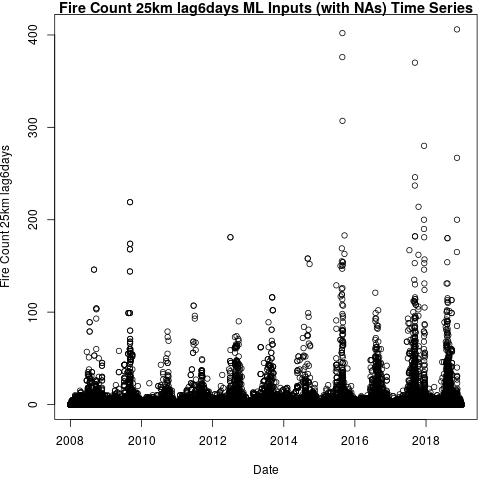
\includegraphics[width=0.77\textwidth]{Code_Outputs/Report_ML_input_PM25_Step4_part_f_de_duplicated_aves_prioritize_24hr_obswNAs_Fire_Count_25km_lag6daysvDate.jpg} 
\caption{\label{fig:Report_ML_input_PM25_Step4_part_f_de_duplicated_aves_prioritize_24hr_obswNAsFire_Count_25km_lag6daysvDate}ML Inputs (with NAs) Time Series} 
\end{figure} 
 

\begin{figure} 
\centering  
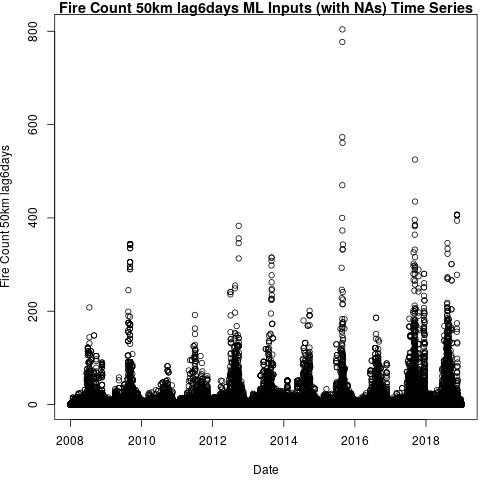
\includegraphics[width=0.77\textwidth]{Code_Outputs/Report_ML_input_PM25_Step4_part_f_de_duplicated_aves_prioritize_24hr_obswNAs_Fire_Count_50km_lag6daysvDate.jpg} 
\caption{\label{fig:Report_ML_input_PM25_Step4_part_f_de_duplicated_aves_prioritize_24hr_obswNAsFire_Count_50km_lag6daysvDate}ML Inputs (with NAs) Time Series} 
\end{figure} 
 

\begin{figure} 
\centering  
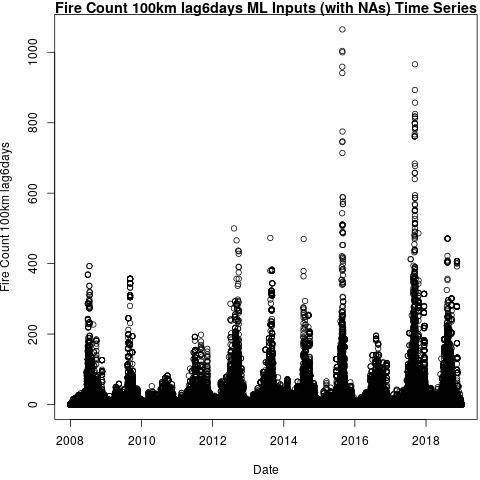
\includegraphics[width=0.77\textwidth]{Code_Outputs/Report_ML_input_PM25_Step4_part_f_de_duplicated_aves_prioritize_24hr_obswNAs_Fire_Count_100km_lag6daysvDate.jpg} 
\caption{\label{fig:Report_ML_input_PM25_Step4_part_f_de_duplicated_aves_prioritize_24hr_obswNAsFire_Count_100km_lag6daysvDate}ML Inputs (with NAs) Time Series} 
\end{figure} 
 

\begin{figure} 
\centering  
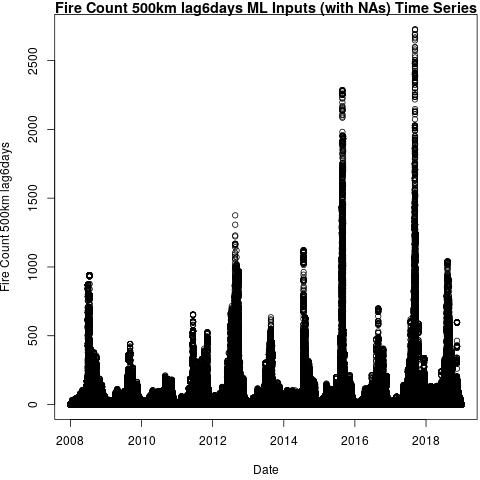
\includegraphics[width=0.77\textwidth]{Code_Outputs/Report_ML_input_PM25_Step4_part_f_de_duplicated_aves_prioritize_24hr_obswNAs_Fire_Count_500km_lag6daysvDate.jpg} 
\caption{\label{fig:Report_ML_input_PM25_Step4_part_f_de_duplicated_aves_prioritize_24hr_obswNAsFire_Count_500km_lag6daysvDate}ML Inputs (with NAs) Time Series} 
\end{figure} 
 

\begin{figure} 
\centering  
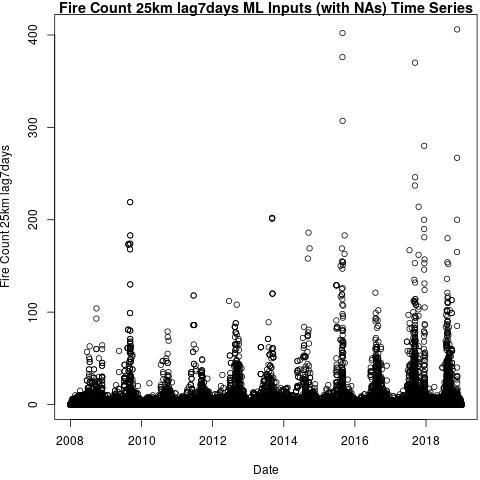
\includegraphics[width=0.77\textwidth]{Code_Outputs/Report_ML_input_PM25_Step4_part_f_de_duplicated_aves_prioritize_24hr_obswNAs_Fire_Count_25km_lag7daysvDate.jpg} 
\caption{\label{fig:Report_ML_input_PM25_Step4_part_f_de_duplicated_aves_prioritize_24hr_obswNAsFire_Count_25km_lag7daysvDate}ML Inputs (with NAs) Time Series} 
\end{figure} 
 

\begin{figure} 
\centering  
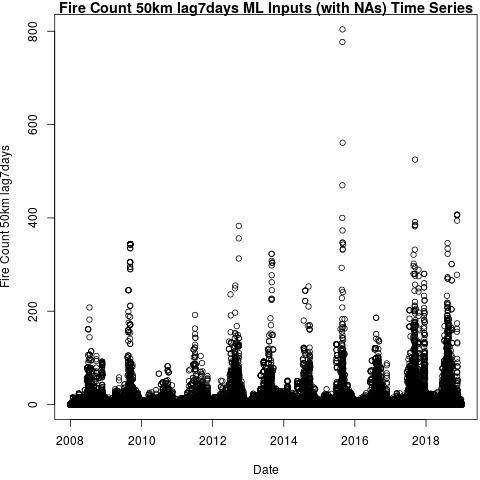
\includegraphics[width=0.77\textwidth]{Code_Outputs/Report_ML_input_PM25_Step4_part_f_de_duplicated_aves_prioritize_24hr_obswNAs_Fire_Count_50km_lag7daysvDate.jpg} 
\caption{\label{fig:Report_ML_input_PM25_Step4_part_f_de_duplicated_aves_prioritize_24hr_obswNAsFire_Count_50km_lag7daysvDate}ML Inputs (with NAs) Time Series} 
\end{figure} 
 

\begin{figure} 
\centering  
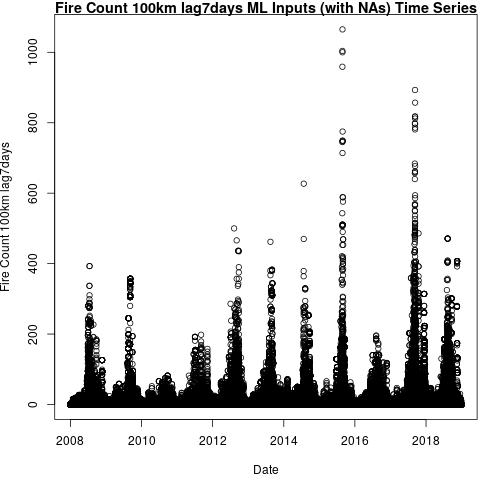
\includegraphics[width=0.77\textwidth]{Code_Outputs/Report_ML_input_PM25_Step4_part_f_de_duplicated_aves_prioritize_24hr_obswNAs_Fire_Count_100km_lag7daysvDate.jpg} 
\caption{\label{fig:Report_ML_input_PM25_Step4_part_f_de_duplicated_aves_prioritize_24hr_obswNAsFire_Count_100km_lag7daysvDate}ML Inputs (with NAs) Time Series} 
\end{figure} 
 

\begin{figure} 
\centering  
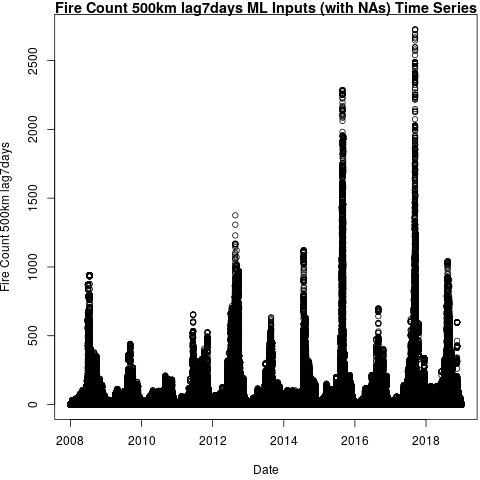
\includegraphics[width=0.77\textwidth]{Code_Outputs/Report_ML_input_PM25_Step4_part_f_de_duplicated_aves_prioritize_24hr_obswNAs_Fire_Count_500km_lag7daysvDate.jpg} 
\caption{\label{fig:Report_ML_input_PM25_Step4_part_f_de_duplicated_aves_prioritize_24hr_obswNAsFire_Count_500km_lag7daysvDate}ML Inputs (with NAs) Time Series} 
\end{figure} 
 

\clearpage 

\begin{figure} 
\centering  
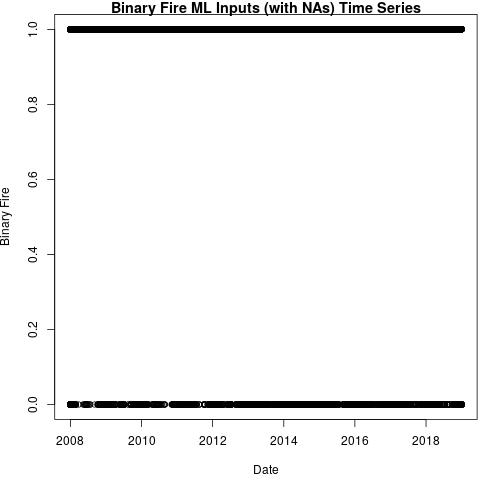
\includegraphics[width=0.77\textwidth]{Code_Outputs/Report_ML_input_PM25_Step4_part_f_de_duplicated_aves_prioritize_24hr_obswNAs_Binary_FirevDate.jpg} 
\caption{\label{fig:Report_ML_input_PM25_Step4_part_f_de_duplicated_aves_prioritize_24hr_obswNAsBinary_FirevDate}ML Inputs (with NAs) Time Series} 
\end{figure} 
 

\begin{figure} 
\centering  
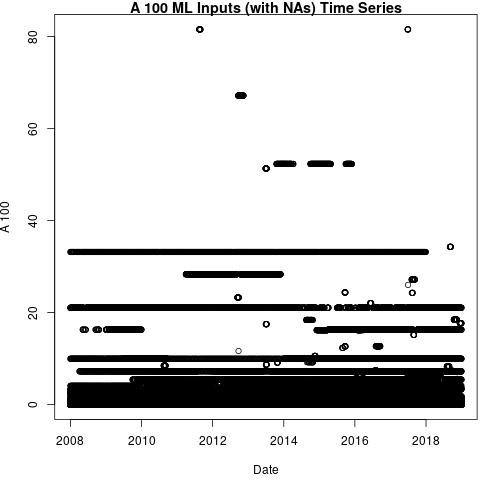
\includegraphics[width=0.77\textwidth]{Code_Outputs/Report_ML_input_PM25_Step4_part_f_de_duplicated_aves_prioritize_24hr_obswNAs_A_100vDate.jpg} 
\caption{\label{fig:Report_ML_input_PM25_Step4_part_f_de_duplicated_aves_prioritize_24hr_obswNAsA_100vDate}ML Inputs (with NAs) Time Series} 
\end{figure} 
 

\begin{figure} 
\centering  
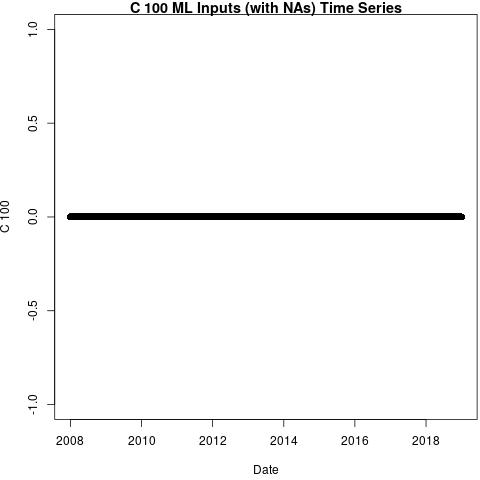
\includegraphics[width=0.77\textwidth]{Code_Outputs/Report_ML_input_PM25_Step4_part_f_de_duplicated_aves_prioritize_24hr_obswNAs_C_100vDate.jpg} 
\caption{\label{fig:Report_ML_input_PM25_Step4_part_f_de_duplicated_aves_prioritize_24hr_obswNAsC_100vDate}ML Inputs (with NAs) Time Series} 
\end{figure} 
 

\begin{figure} 
\centering  
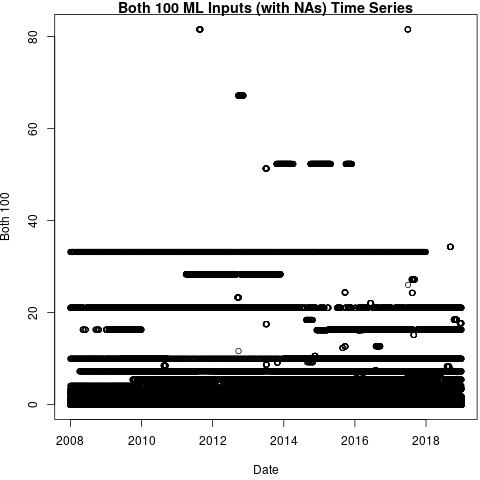
\includegraphics[width=0.77\textwidth]{Code_Outputs/Report_ML_input_PM25_Step4_part_f_de_duplicated_aves_prioritize_24hr_obswNAs_Both_100vDate.jpg} 
\caption{\label{fig:Report_ML_input_PM25_Step4_part_f_de_duplicated_aves_prioritize_24hr_obswNAsBoth_100vDate}ML Inputs (with NAs) Time Series} 
\end{figure} 
 

\begin{figure} 
\centering  
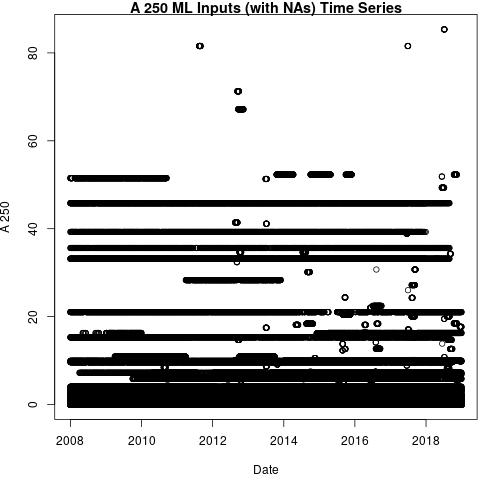
\includegraphics[width=0.77\textwidth]{Code_Outputs/Report_ML_input_PM25_Step4_part_f_de_duplicated_aves_prioritize_24hr_obswNAs_A_250vDate.jpg} 
\caption{\label{fig:Report_ML_input_PM25_Step4_part_f_de_duplicated_aves_prioritize_24hr_obswNAsA_250vDate}ML Inputs (with NAs) Time Series} 
\end{figure} 
 

\begin{figure} 
\centering  
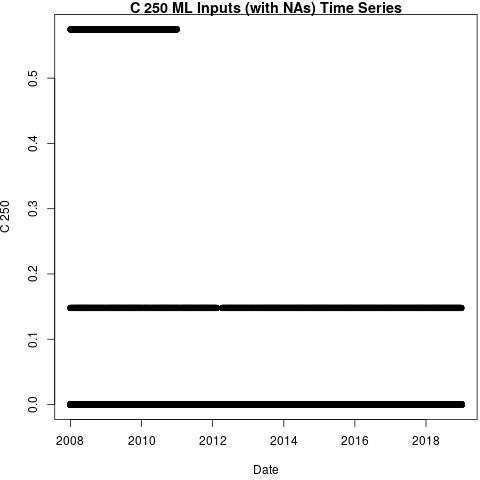
\includegraphics[width=0.77\textwidth]{Code_Outputs/Report_ML_input_PM25_Step4_part_f_de_duplicated_aves_prioritize_24hr_obswNAs_C_250vDate.jpg} 
\caption{\label{fig:Report_ML_input_PM25_Step4_part_f_de_duplicated_aves_prioritize_24hr_obswNAsC_250vDate}ML Inputs (with NAs) Time Series} 
\end{figure} 
 

\begin{figure} 
\centering  
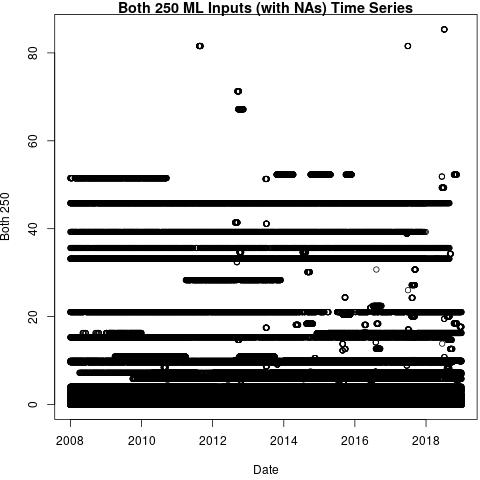
\includegraphics[width=0.77\textwidth]{Code_Outputs/Report_ML_input_PM25_Step4_part_f_de_duplicated_aves_prioritize_24hr_obswNAs_Both_250vDate.jpg} 
\caption{\label{fig:Report_ML_input_PM25_Step4_part_f_de_duplicated_aves_prioritize_24hr_obswNAsBoth_250vDate}ML Inputs (with NAs) Time Series} 
\end{figure} 
 

\begin{figure} 
\centering  
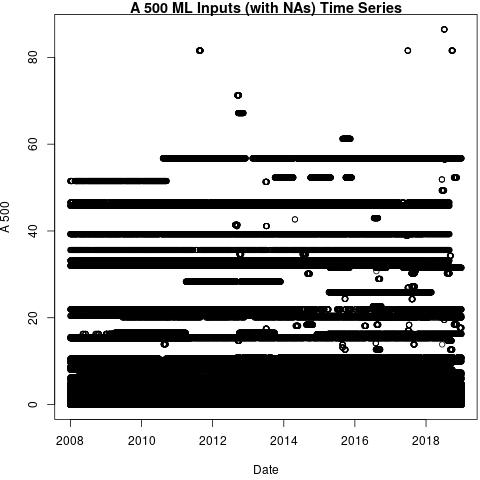
\includegraphics[width=0.77\textwidth]{Code_Outputs/Report_ML_input_PM25_Step4_part_f_de_duplicated_aves_prioritize_24hr_obswNAs_A_500vDate.jpg} 
\caption{\label{fig:Report_ML_input_PM25_Step4_part_f_de_duplicated_aves_prioritize_24hr_obswNAsA_500vDate}ML Inputs (with NAs) Time Series} 
\end{figure} 
 

\begin{figure} 
\centering  
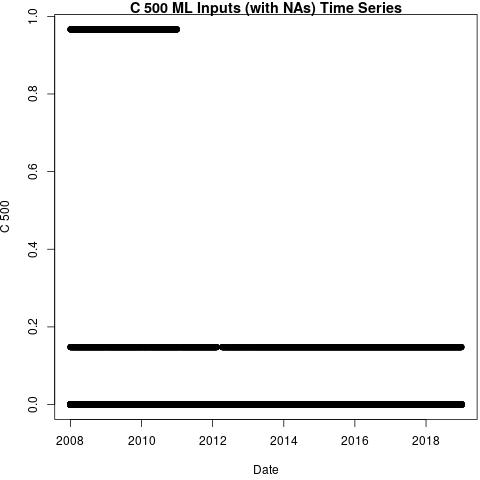
\includegraphics[width=0.77\textwidth]{Code_Outputs/Report_ML_input_PM25_Step4_part_f_de_duplicated_aves_prioritize_24hr_obswNAs_C_500vDate.jpg} 
\caption{\label{fig:Report_ML_input_PM25_Step4_part_f_de_duplicated_aves_prioritize_24hr_obswNAsC_500vDate}ML Inputs (with NAs) Time Series} 
\end{figure} 
 

\begin{figure} 
\centering  
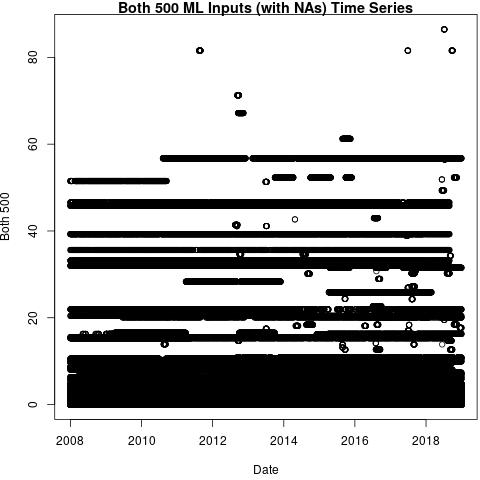
\includegraphics[width=0.77\textwidth]{Code_Outputs/Report_ML_input_PM25_Step4_part_f_de_duplicated_aves_prioritize_24hr_obswNAs_Both_500vDate.jpg} 
\caption{\label{fig:Report_ML_input_PM25_Step4_part_f_de_duplicated_aves_prioritize_24hr_obswNAsBoth_500vDate}ML Inputs (with NAs) Time Series} 
\end{figure} 
 

\clearpage 

\begin{figure} 
\centering  
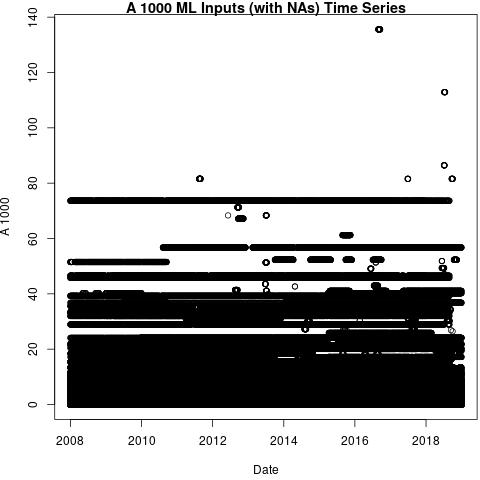
\includegraphics[width=0.77\textwidth]{Code_Outputs/Report_ML_input_PM25_Step4_part_f_de_duplicated_aves_prioritize_24hr_obswNAs_A_1000vDate.jpg} 
\caption{\label{fig:Report_ML_input_PM25_Step4_part_f_de_duplicated_aves_prioritize_24hr_obswNAsA_1000vDate}ML Inputs (with NAs) Time Series} 
\end{figure} 
 

\begin{figure} 
\centering  
\includegraphics[width=0.77\textwidth]{Code_Outputs/Report_ML_input_PM25_Step4_part_f_de_duplicated_aves_prioritize_24hr_obswNAs_C_1000vDate.jpg} 
\caption{\label{fig:Report_ML_input_PM25_Step4_part_f_de_duplicated_aves_prioritize_24hr_obswNAsC_1000vDate}ML Inputs (with NAs) Time Series} 
\end{figure} 
 

\begin{figure} 
\centering  
\includegraphics[width=0.77\textwidth]{Code_Outputs/Report_ML_input_PM25_Step4_part_f_de_duplicated_aves_prioritize_24hr_obswNAs_Both_1000vDate.jpg} 
\caption{\label{fig:Report_ML_input_PM25_Step4_part_f_de_duplicated_aves_prioritize_24hr_obswNAsBoth_1000vDate}ML Inputs (with NAs) Time Series} 
\end{figure} 
 

\begin{figure} 
\centering  
\includegraphics[width=0.77\textwidth]{Code_Outputs/Report_ML_input_PM25_Step4_part_f_de_duplicated_aves_prioritize_24hr_obswNAs_Pop_densityvDate.jpg} 
\caption{\label{fig:Report_ML_input_PM25_Step4_part_f_de_duplicated_aves_prioritize_24hr_obswNAsPop_densityvDate}ML Inputs (with NAs) Time Series} 
\end{figure} 
 

\begin{figure} 
\centering  
\includegraphics[width=0.77\textwidth]{Code_Outputs/Report_ML_input_PM25_Step4_part_f_de_duplicated_aves_prioritize_24hr_obswNAs_MAIAC_AODvDate.jpg} 
\caption{\label{fig:Report_ML_input_PM25_Step4_part_f_de_duplicated_aves_prioritize_24hr_obswNAsMAIAC_AODvDate}ML Inputs (with NAs) Time Series} 
\end{figure} 
 

\begin{figure} 
\centering  
\includegraphics[width=0.77\textwidth]{Code_Outputs/Report_ML_input_PM25_Step4_part_f_de_duplicated_aves_prioritize_24hr_obswNAs_elevationvDate.jpg} 
\caption{\label{fig:Report_ML_input_PM25_Step4_part_f_de_duplicated_aves_prioritize_24hr_obswNAselevationvDate}ML Inputs (with NAs) Time Series} 
\end{figure} 
 

\begin{figure} 
\centering  
\includegraphics[width=0.77\textwidth]{Code_Outputs/Report_ML_input_PM25_Step4_part_f_de_duplicated_aves_prioritize_24hr_obswNAs_HPBLsurfacevDate.jpg} 
\caption{\label{fig:Report_ML_input_PM25_Step4_part_f_de_duplicated_aves_prioritize_24hr_obswNAsHPBLsurfacevDate}ML Inputs (with NAs) Time Series} 
\end{figure} 
 

\begin{figure} 
\centering  
\includegraphics[width=0.77\textwidth]{Code_Outputs/Report_ML_input_PM25_Step4_part_f_de_duplicated_aves_prioritize_24hr_obswNAs_TMP2mabovegroundvDate.jpg} 
\caption{\label{fig:Report_ML_input_PM25_Step4_part_f_de_duplicated_aves_prioritize_24hr_obswNAsTMP2mabovegroundvDate}ML Inputs (with NAs) Time Series} 
\end{figure} 
 

\begin{figure} 
\centering  
\includegraphics[width=0.77\textwidth]{Code_Outputs/Report_ML_input_PM25_Step4_part_f_de_duplicated_aves_prioritize_24hr_obswNAs_RH2mabovegroundvDate.jpg} 
\caption{\label{fig:Report_ML_input_PM25_Step4_part_f_de_duplicated_aves_prioritize_24hr_obswNAsRH2mabovegroundvDate}ML Inputs (with NAs) Time Series} 
\end{figure} 
 

\begin{figure} 
\centering  
\includegraphics[width=0.77\textwidth]{Code_Outputs/Report_ML_input_PM25_Step4_part_f_de_duplicated_aves_prioritize_24hr_obswNAs_DPT2mabovegroundvDate.jpg} 
\caption{\label{fig:Report_ML_input_PM25_Step4_part_f_de_duplicated_aves_prioritize_24hr_obswNAsDPT2mabovegroundvDate}ML Inputs (with NAs) Time Series} 
\end{figure} 
 

\clearpage 

\begin{figure} 
\centering  
\includegraphics[width=0.77\textwidth]{Code_Outputs/Report_ML_input_PM25_Step4_part_f_de_duplicated_aves_prioritize_24hr_obswNAs_APCPsurfacevDate.jpg} 
\caption{\label{fig:Report_ML_input_PM25_Step4_part_f_de_duplicated_aves_prioritize_24hr_obswNAsAPCPsurfacevDate}ML Inputs (with NAs) Time Series} 
\end{figure} 
 

\begin{figure} 
\centering  
\includegraphics[width=0.77\textwidth]{Code_Outputs/Report_ML_input_PM25_Step4_part_f_de_duplicated_aves_prioritize_24hr_obswNAs_WEASDsurfacevDate.jpg} 
\caption{\label{fig:Report_ML_input_PM25_Step4_part_f_de_duplicated_aves_prioritize_24hr_obswNAsWEASDsurfacevDate}ML Inputs (with NAs) Time Series} 
\end{figure} 
 

\begin{figure} 
\centering  
\includegraphics[width=0.77\textwidth]{Code_Outputs/Report_ML_input_PM25_Step4_part_f_de_duplicated_aves_prioritize_24hr_obswNAs_SNOWCsurfacevDate.jpg} 
\caption{\label{fig:Report_ML_input_PM25_Step4_part_f_de_duplicated_aves_prioritize_24hr_obswNAsSNOWCsurfacevDate}ML Inputs (with NAs) Time Series} 
\end{figure} 
 

\begin{figure} 
\centering  
\includegraphics[width=0.77\textwidth]{Code_Outputs/Report_ML_input_PM25_Step4_part_f_de_duplicated_aves_prioritize_24hr_obswNAs_UGRD10mabovegroundvDate.jpg} 
\caption{\label{fig:Report_ML_input_PM25_Step4_part_f_de_duplicated_aves_prioritize_24hr_obswNAsUGRD10mabovegroundvDate}ML Inputs (with NAs) Time Series} 
\end{figure} 
 

\begin{figure} 
\centering  
\includegraphics[width=0.77\textwidth]{Code_Outputs/Report_ML_input_PM25_Step4_part_f_de_duplicated_aves_prioritize_24hr_obswNAs_VGRD10mabovegroundvDate.jpg} 
\caption{\label{fig:Report_ML_input_PM25_Step4_part_f_de_duplicated_aves_prioritize_24hr_obswNAsVGRD10mabovegroundvDate}ML Inputs (with NAs) Time Series} 
\end{figure} 
 

\begin{figure} 
\centering  
\includegraphics[width=0.77\textwidth]{Code_Outputs/Report_ML_input_PM25_Step4_part_f_de_duplicated_aves_prioritize_24hr_obswNAs_PRMSLmeansealevelvDate.jpg} 
\caption{\label{fig:Report_ML_input_PM25_Step4_part_f_de_duplicated_aves_prioritize_24hr_obswNAsPRMSLmeansealevelvDate}ML Inputs (with NAs) Time Series} 
\end{figure} 
 

\begin{figure} 
\centering  
\includegraphics[width=0.77\textwidth]{Code_Outputs/Report_ML_input_PM25_Step4_part_f_de_duplicated_aves_prioritize_24hr_obswNAs_PRESsurfacevDate.jpg} 
\caption{\label{fig:Report_ML_input_PM25_Step4_part_f_de_duplicated_aves_prioritize_24hr_obswNAsPRESsurfacevDate}ML Inputs (with NAs) Time Series} 
\end{figure} 
 

\begin{figure} 
\centering  
\includegraphics[width=0.77\textwidth]{Code_Outputs/Report_ML_input_PM25_Step4_part_f_de_duplicated_aves_prioritize_24hr_obswNAs_DZDT850mbvDate.jpg} 
\caption{\label{fig:Report_ML_input_PM25_Step4_part_f_de_duplicated_aves_prioritize_24hr_obswNAsDZDT850mbvDate}ML Inputs (with NAs) Time Series} 
\end{figure} 
 

\begin{figure} 
\centering  
\includegraphics[width=0.77\textwidth]{Code_Outputs/Report_ML_input_PM25_Step4_part_f_de_duplicated_aves_prioritize_24hr_obswNAs_DZDT700mbvDate.jpg} 
\caption{\label{fig:Report_ML_input_PM25_Step4_part_f_de_duplicated_aves_prioritize_24hr_obswNAsDZDT700mbvDate}ML Inputs (with NAs) Time Series} 
\end{figure} 
 

\begin{figure} 
\centering  
\includegraphics[width=0.77\textwidth]{Code_Outputs/Report_ML_input_PM25_Step4_part_f_de_duplicated_aves_prioritize_24hr_obswNAs_NLCD_1km_percent_urban_buffervDate.jpg} 
\caption{\label{fig:Report_ML_input_PM25_Step4_part_f_de_duplicated_aves_prioritize_24hr_obswNAsNLCD_1km_percent_urban_buffervDate}ML Inputs (with NAs) Time Series} 
\end{figure} 
 

\clearpage 

\begin{figure} 
\centering  
\includegraphics[width=0.77\textwidth]{Code_Outputs/Report_ML_input_PM25_Step4_part_f_de_duplicated_aves_prioritize_24hr_obswNAs_NLCD_5km_percent_urban_buffervDate.jpg} 
\caption{\label{fig:Report_ML_input_PM25_Step4_part_f_de_duplicated_aves_prioritize_24hr_obswNAsNLCD_5km_percent_urban_buffervDate}ML Inputs (with NAs) Time Series} 
\end{figure} 
 

\begin{figure} 
\centering  
\includegraphics[width=0.77\textwidth]{Code_Outputs/Report_ML_input_PM25_Step4_part_f_de_duplicated_aves_prioritize_24hr_obswNAs_NLCD_10km_percent_urban_buffervDate.jpg} 
\caption{\label{fig:Report_ML_input_PM25_Step4_part_f_de_duplicated_aves_prioritize_24hr_obswNAsNLCD_10km_percent_urban_buffervDate}ML Inputs (with NAs) Time Series} 
\end{figure} 
 

\begin{figure} 
\centering  
\includegraphics[width=0.77\textwidth]{Code_Outputs/Report_ML_input_PM25_Step4_part_f_de_duplicated_aves_prioritize_24hr_obswNAs_NDVIvDate.jpg} 
\caption{\label{fig:Report_ML_input_PM25_Step4_part_f_de_duplicated_aves_prioritize_24hr_obswNAsNDVIvDate}ML Inputs (with NAs) Time Series} 
\end{figure} 
 

\begin{figure} 
\centering  
\includegraphics[width=0.77\textwidth]{Code_Outputs/Report_ML_input_PM25_Step4_part_f_de_duplicated_aves_prioritize_24hr_obswNAs_DayOfWeekvDate.jpg} 
\caption{\label{fig:Report_ML_input_PM25_Step4_part_f_de_duplicated_aves_prioritize_24hr_obswNAsDayOfWeekvDate}ML Inputs (with NAs) Time Series} 
\end{figure} 
 

\begin{figure} 
\centering  
\includegraphics[width=0.77\textwidth]{Code_Outputs/Report_ML_input_PM25_Step4_part_f_de_duplicated_aves_prioritize_24hr_obswNAs_WintervDate.jpg} 
\caption{\label{fig:Report_ML_input_PM25_Step4_part_f_de_duplicated_aves_prioritize_24hr_obswNAsWintervDate}ML Inputs (with NAs) Time Series} 
\end{figure} 
 

\begin{figure} 
\centering  
\includegraphics[width=0.77\textwidth]{Code_Outputs/Report_ML_input_PM25_Step4_part_f_de_duplicated_aves_prioritize_24hr_obswNAs_SpringvDate.jpg} 
\caption{\label{fig:Report_ML_input_PM25_Step4_part_f_de_duplicated_aves_prioritize_24hr_obswNAsSpringvDate}ML Inputs (with NAs) Time Series} 
\end{figure} 
 

\begin{figure} 
\centering  
\includegraphics[width=0.77\textwidth]{Code_Outputs/Report_ML_input_PM25_Step4_part_f_de_duplicated_aves_prioritize_24hr_obswNAs_SummervDate.jpg} 
\caption{\label{fig:Report_ML_input_PM25_Step4_part_f_de_duplicated_aves_prioritize_24hr_obswNAsSummervDate}ML Inputs (with NAs) Time Series} 
\end{figure} 
 

\begin{figure} 
\centering  
\includegraphics[width=0.77\textwidth]{Code_Outputs/Report_ML_input_PM25_Step4_part_f_de_duplicated_aves_prioritize_24hr_obswNAs_FallvDate.jpg} 
\caption{\label{fig:Report_ML_input_PM25_Step4_part_f_de_duplicated_aves_prioritize_24hr_obswNAsFallvDate}ML Inputs (with NAs) Time Series} 
\end{figure} 
 

\begin{figure} 
\centering  
\includegraphics[width=0.77\textwidth]{Code_Outputs/Report_ML_input_PM25_Step4_part_f_de_duplicated_aves_prioritize_24hr_obswNAs_StatevDate.jpg} 
\caption{\label{fig:Report_ML_input_PM25_Step4_part_f_de_duplicated_aves_prioritize_24hr_obswNAsStatevDate}ML Inputs (with NAs) Time Series} 
\end{figure} 
 

\begin{figure} 
\centering  
\includegraphics[width=0.77\textwidth]{Code_Outputs/Report_ML_input_PM25_Step4_part_f_de_duplicated_aves_prioritize_24hr_obswNAs_CosDOYvDate.jpg} 
\caption{\label{fig:Report_ML_input_PM25_Step4_part_f_de_duplicated_aves_prioritize_24hr_obswNAsCosDOYvDate}ML Inputs (with NAs) Time Series} 
\end{figure} 
 
 

% PM2.5 vs predictor for each predictor variable 

\subsection{ML Inputs (with NAs) Plot against PM2.5 Obs Images} 
 

\begin{figure} 
\centering  
\includegraphics[width=0.77\textwidth]{Code_Outputs/Report_ML_input_PM25_Step4_part_f_de_duplicated_aves_prioritize_24hr_obswNAs_Fire_Count_25km_lag0daysvPM25_Obs.jpg} 
\caption{\label{fig:Report_ML_input_PM25_Step4_part_f_de_duplicated_aves_prioritize_24hr_obswNAsFire_Count_25km_lag0daysvPM25_Obs}ML Inputs (with NAs) Plot against PM2.5 Obs} 
\end{figure} 
 

\begin{figure} 
\centering  
\includegraphics[width=0.77\textwidth]{Code_Outputs/Report_ML_input_PM25_Step4_part_f_de_duplicated_aves_prioritize_24hr_obswNAs_Fire_Count_50km_lag0daysvPM25_Obs.jpg} 
\caption{\label{fig:Report_ML_input_PM25_Step4_part_f_de_duplicated_aves_prioritize_24hr_obswNAsFire_Count_50km_lag0daysvPM25_Obs}ML Inputs (with NAs) Plot against PM2.5 Obs} 
\end{figure} 
 

\begin{figure} 
\centering  
\includegraphics[width=0.77\textwidth]{Code_Outputs/Report_ML_input_PM25_Step4_part_f_de_duplicated_aves_prioritize_24hr_obswNAs_Fire_Count_100km_lag0daysvPM25_Obs.jpg} 
\caption{\label{fig:Report_ML_input_PM25_Step4_part_f_de_duplicated_aves_prioritize_24hr_obswNAsFire_Count_100km_lag0daysvPM25_Obs}ML Inputs (with NAs) Plot against PM2.5 Obs} 
\end{figure} 
 

\begin{figure} 
\centering  
\includegraphics[width=0.77\textwidth]{Code_Outputs/Report_ML_input_PM25_Step4_part_f_de_duplicated_aves_prioritize_24hr_obswNAs_Fire_Count_500km_lag0daysvPM25_Obs.jpg} 
\caption{\label{fig:Report_ML_input_PM25_Step4_part_f_de_duplicated_aves_prioritize_24hr_obswNAsFire_Count_500km_lag0daysvPM25_Obs}ML Inputs (with NAs) Plot against PM2.5 Obs} 
\end{figure} 
 

\begin{figure} 
\centering  
\includegraphics[width=0.77\textwidth]{Code_Outputs/Report_ML_input_PM25_Step4_part_f_de_duplicated_aves_prioritize_24hr_obswNAs_Fire_Count_25km_lag1daysvPM25_Obs.jpg} 
\caption{\label{fig:Report_ML_input_PM25_Step4_part_f_de_duplicated_aves_prioritize_24hr_obswNAsFire_Count_25km_lag1daysvPM25_Obs}ML Inputs (with NAs) Plot against PM2.5 Obs} 
\end{figure} 
 

\begin{figure} 
\centering  
\includegraphics[width=0.77\textwidth]{Code_Outputs/Report_ML_input_PM25_Step4_part_f_de_duplicated_aves_prioritize_24hr_obswNAs_Fire_Count_50km_lag1daysvPM25_Obs.jpg} 
\caption{\label{fig:Report_ML_input_PM25_Step4_part_f_de_duplicated_aves_prioritize_24hr_obswNAsFire_Count_50km_lag1daysvPM25_Obs}ML Inputs (with NAs) Plot against PM2.5 Obs} 
\end{figure} 
 

\begin{figure} 
\centering  
\includegraphics[width=0.77\textwidth]{Code_Outputs/Report_ML_input_PM25_Step4_part_f_de_duplicated_aves_prioritize_24hr_obswNAs_Fire_Count_100km_lag1daysvPM25_Obs.jpg} 
\caption{\label{fig:Report_ML_input_PM25_Step4_part_f_de_duplicated_aves_prioritize_24hr_obswNAsFire_Count_100km_lag1daysvPM25_Obs}ML Inputs (with NAs) Plot against PM2.5 Obs} 
\end{figure} 
 

\begin{figure} 
\centering  
\includegraphics[width=0.77\textwidth]{Code_Outputs/Report_ML_input_PM25_Step4_part_f_de_duplicated_aves_prioritize_24hr_obswNAs_Fire_Count_500km_lag1daysvPM25_Obs.jpg} 
\caption{\label{fig:Report_ML_input_PM25_Step4_part_f_de_duplicated_aves_prioritize_24hr_obswNAsFire_Count_500km_lag1daysvPM25_Obs}ML Inputs (with NAs) Plot against PM2.5 Obs} 
\end{figure} 
 

\begin{figure} 
\centering  
\includegraphics[width=0.77\textwidth]{Code_Outputs/Report_ML_input_PM25_Step4_part_f_de_duplicated_aves_prioritize_24hr_obswNAs_Fire_Count_25km_lag2daysvPM25_Obs.jpg} 
\caption{\label{fig:Report_ML_input_PM25_Step4_part_f_de_duplicated_aves_prioritize_24hr_obswNAsFire_Count_25km_lag2daysvPM25_Obs}ML Inputs (with NAs) Plot against PM2.5 Obs} 
\end{figure} 
 

\clearpage 

\begin{figure} 
\centering  
\includegraphics[width=0.77\textwidth]{Code_Outputs/Report_ML_input_PM25_Step4_part_f_de_duplicated_aves_prioritize_24hr_obswNAs_Fire_Count_50km_lag2daysvPM25_Obs.jpg} 
\caption{\label{fig:Report_ML_input_PM25_Step4_part_f_de_duplicated_aves_prioritize_24hr_obswNAsFire_Count_50km_lag2daysvPM25_Obs}ML Inputs (with NAs) Plot against PM2.5 Obs} 
\end{figure} 
 

\begin{figure} 
\centering  
\includegraphics[width=0.77\textwidth]{Code_Outputs/Report_ML_input_PM25_Step4_part_f_de_duplicated_aves_prioritize_24hr_obswNAs_Fire_Count_100km_lag2daysvPM25_Obs.jpg} 
\caption{\label{fig:Report_ML_input_PM25_Step4_part_f_de_duplicated_aves_prioritize_24hr_obswNAsFire_Count_100km_lag2daysvPM25_Obs}ML Inputs (with NAs) Plot against PM2.5 Obs} 
\end{figure} 
 

\begin{figure} 
\centering  
\includegraphics[width=0.77\textwidth]{Code_Outputs/Report_ML_input_PM25_Step4_part_f_de_duplicated_aves_prioritize_24hr_obswNAs_Fire_Count_500km_lag2daysvPM25_Obs.jpg} 
\caption{\label{fig:Report_ML_input_PM25_Step4_part_f_de_duplicated_aves_prioritize_24hr_obswNAsFire_Count_500km_lag2daysvPM25_Obs}ML Inputs (with NAs) Plot against PM2.5 Obs} 
\end{figure} 
 

\begin{figure} 
\centering  
\includegraphics[width=0.77\textwidth]{Code_Outputs/Report_ML_input_PM25_Step4_part_f_de_duplicated_aves_prioritize_24hr_obswNAs_Fire_Count_25km_lag3daysvPM25_Obs.jpg} 
\caption{\label{fig:Report_ML_input_PM25_Step4_part_f_de_duplicated_aves_prioritize_24hr_obswNAsFire_Count_25km_lag3daysvPM25_Obs}ML Inputs (with NAs) Plot against PM2.5 Obs} 
\end{figure} 
 

\begin{figure} 
\centering  
\includegraphics[width=0.77\textwidth]{Code_Outputs/Report_ML_input_PM25_Step4_part_f_de_duplicated_aves_prioritize_24hr_obswNAs_Fire_Count_50km_lag3daysvPM25_Obs.jpg} 
\caption{\label{fig:Report_ML_input_PM25_Step4_part_f_de_duplicated_aves_prioritize_24hr_obswNAsFire_Count_50km_lag3daysvPM25_Obs}ML Inputs (with NAs) Plot against PM2.5 Obs} 
\end{figure} 
 

\begin{figure} 
\centering  
\includegraphics[width=0.77\textwidth]{Code_Outputs/Report_ML_input_PM25_Step4_part_f_de_duplicated_aves_prioritize_24hr_obswNAs_Fire_Count_100km_lag3daysvPM25_Obs.jpg} 
\caption{\label{fig:Report_ML_input_PM25_Step4_part_f_de_duplicated_aves_prioritize_24hr_obswNAsFire_Count_100km_lag3daysvPM25_Obs}ML Inputs (with NAs) Plot against PM2.5 Obs} 
\end{figure} 
 

\begin{figure} 
\centering  
\includegraphics[width=0.77\textwidth]{Code_Outputs/Report_ML_input_PM25_Step4_part_f_de_duplicated_aves_prioritize_24hr_obswNAs_Fire_Count_500km_lag3daysvPM25_Obs.jpg} 
\caption{\label{fig:Report_ML_input_PM25_Step4_part_f_de_duplicated_aves_prioritize_24hr_obswNAsFire_Count_500km_lag3daysvPM25_Obs}ML Inputs (with NAs) Plot against PM2.5 Obs} 
\end{figure} 
 

\begin{figure} 
\centering  
\includegraphics[width=0.77\textwidth]{Code_Outputs/Report_ML_input_PM25_Step4_part_f_de_duplicated_aves_prioritize_24hr_obswNAs_Fire_Count_25km_lag4daysvPM25_Obs.jpg} 
\caption{\label{fig:Report_ML_input_PM25_Step4_part_f_de_duplicated_aves_prioritize_24hr_obswNAsFire_Count_25km_lag4daysvPM25_Obs}ML Inputs (with NAs) Plot against PM2.5 Obs} 
\end{figure} 
 

\begin{figure} 
\centering  
\includegraphics[width=0.77\textwidth]{Code_Outputs/Report_ML_input_PM25_Step4_part_f_de_duplicated_aves_prioritize_24hr_obswNAs_Fire_Count_50km_lag4daysvPM25_Obs.jpg} 
\caption{\label{fig:Report_ML_input_PM25_Step4_part_f_de_duplicated_aves_prioritize_24hr_obswNAsFire_Count_50km_lag4daysvPM25_Obs}ML Inputs (with NAs) Plot against PM2.5 Obs} 
\end{figure} 
 

\begin{figure} 
\centering  
\includegraphics[width=0.77\textwidth]{Code_Outputs/Report_ML_input_PM25_Step4_part_f_de_duplicated_aves_prioritize_24hr_obswNAs_Fire_Count_100km_lag4daysvPM25_Obs.jpg} 
\caption{\label{fig:Report_ML_input_PM25_Step4_part_f_de_duplicated_aves_prioritize_24hr_obswNAsFire_Count_100km_lag4daysvPM25_Obs}ML Inputs (with NAs) Plot against PM2.5 Obs} 
\end{figure} 
 

\clearpage 

\begin{figure} 
\centering  
\includegraphics[width=0.77\textwidth]{Code_Outputs/Report_ML_input_PM25_Step4_part_f_de_duplicated_aves_prioritize_24hr_obswNAs_Fire_Count_500km_lag4daysvPM25_Obs.jpg} 
\caption{\label{fig:Report_ML_input_PM25_Step4_part_f_de_duplicated_aves_prioritize_24hr_obswNAsFire_Count_500km_lag4daysvPM25_Obs}ML Inputs (with NAs) Plot against PM2.5 Obs} 
\end{figure} 
 

\begin{figure} 
\centering  
\includegraphics[width=0.77\textwidth]{Code_Outputs/Report_ML_input_PM25_Step4_part_f_de_duplicated_aves_prioritize_24hr_obswNAs_Fire_Count_25km_lag5daysvPM25_Obs.jpg} 
\caption{\label{fig:Report_ML_input_PM25_Step4_part_f_de_duplicated_aves_prioritize_24hr_obswNAsFire_Count_25km_lag5daysvPM25_Obs}ML Inputs (with NAs) Plot against PM2.5 Obs} 
\end{figure} 
 

\begin{figure} 
\centering  
\includegraphics[width=0.77\textwidth]{Code_Outputs/Report_ML_input_PM25_Step4_part_f_de_duplicated_aves_prioritize_24hr_obswNAs_Fire_Count_50km_lag5daysvPM25_Obs.jpg} 
\caption{\label{fig:Report_ML_input_PM25_Step4_part_f_de_duplicated_aves_prioritize_24hr_obswNAsFire_Count_50km_lag5daysvPM25_Obs}ML Inputs (with NAs) Plot against PM2.5 Obs} 
\end{figure} 
 

\begin{figure} 
\centering  
\includegraphics[width=0.77\textwidth]{Code_Outputs/Report_ML_input_PM25_Step4_part_f_de_duplicated_aves_prioritize_24hr_obswNAs_Fire_Count_100km_lag5daysvPM25_Obs.jpg} 
\caption{\label{fig:Report_ML_input_PM25_Step4_part_f_de_duplicated_aves_prioritize_24hr_obswNAsFire_Count_100km_lag5daysvPM25_Obs}ML Inputs (with NAs) Plot against PM2.5 Obs} 
\end{figure} 
 

\begin{figure} 
\centering  
\includegraphics[width=0.77\textwidth]{Code_Outputs/Report_ML_input_PM25_Step4_part_f_de_duplicated_aves_prioritize_24hr_obswNAs_Fire_Count_500km_lag5daysvPM25_Obs.jpg} 
\caption{\label{fig:Report_ML_input_PM25_Step4_part_f_de_duplicated_aves_prioritize_24hr_obswNAsFire_Count_500km_lag5daysvPM25_Obs}ML Inputs (with NAs) Plot against PM2.5 Obs} 
\end{figure} 
 

\begin{figure} 
\centering  
\includegraphics[width=0.77\textwidth]{Code_Outputs/Report_ML_input_PM25_Step4_part_f_de_duplicated_aves_prioritize_24hr_obswNAs_Fire_Count_25km_lag6daysvPM25_Obs.jpg} 
\caption{\label{fig:Report_ML_input_PM25_Step4_part_f_de_duplicated_aves_prioritize_24hr_obswNAsFire_Count_25km_lag6daysvPM25_Obs}ML Inputs (with NAs) Plot against PM2.5 Obs} 
\end{figure} 
 

\begin{figure} 
\centering  
\includegraphics[width=0.77\textwidth]{Code_Outputs/Report_ML_input_PM25_Step4_part_f_de_duplicated_aves_prioritize_24hr_obswNAs_Fire_Count_50km_lag6daysvPM25_Obs.jpg} 
\caption{\label{fig:Report_ML_input_PM25_Step4_part_f_de_duplicated_aves_prioritize_24hr_obswNAsFire_Count_50km_lag6daysvPM25_Obs}ML Inputs (with NAs) Plot against PM2.5 Obs} 
\end{figure} 
 

\begin{figure} 
\centering  
\includegraphics[width=0.77\textwidth]{Code_Outputs/Report_ML_input_PM25_Step4_part_f_de_duplicated_aves_prioritize_24hr_obswNAs_Fire_Count_100km_lag6daysvPM25_Obs.jpg} 
\caption{\label{fig:Report_ML_input_PM25_Step4_part_f_de_duplicated_aves_prioritize_24hr_obswNAsFire_Count_100km_lag6daysvPM25_Obs}ML Inputs (with NAs) Plot against PM2.5 Obs} 
\end{figure} 
 

\begin{figure} 
\centering  
\includegraphics[width=0.77\textwidth]{Code_Outputs/Report_ML_input_PM25_Step4_part_f_de_duplicated_aves_prioritize_24hr_obswNAs_Fire_Count_500km_lag6daysvPM25_Obs.jpg} 
\caption{\label{fig:Report_ML_input_PM25_Step4_part_f_de_duplicated_aves_prioritize_24hr_obswNAsFire_Count_500km_lag6daysvPM25_Obs}ML Inputs (with NAs) Plot against PM2.5 Obs} 
\end{figure} 
 

\begin{figure} 
\centering  
\includegraphics[width=0.77\textwidth]{Code_Outputs/Report_ML_input_PM25_Step4_part_f_de_duplicated_aves_prioritize_24hr_obswNAs_Fire_Count_25km_lag7daysvPM25_Obs.jpg} 
\caption{\label{fig:Report_ML_input_PM25_Step4_part_f_de_duplicated_aves_prioritize_24hr_obswNAsFire_Count_25km_lag7daysvPM25_Obs}ML Inputs (with NAs) Plot against PM2.5 Obs} 
\end{figure} 
 

\clearpage 

\begin{figure} 
\centering  
\includegraphics[width=0.77\textwidth]{Code_Outputs/Report_ML_input_PM25_Step4_part_f_de_duplicated_aves_prioritize_24hr_obswNAs_Fire_Count_50km_lag7daysvPM25_Obs.jpg} 
\caption{\label{fig:Report_ML_input_PM25_Step4_part_f_de_duplicated_aves_prioritize_24hr_obswNAsFire_Count_50km_lag7daysvPM25_Obs}ML Inputs (with NAs) Plot against PM2.5 Obs} 
\end{figure} 
 

\begin{figure} 
\centering  
\includegraphics[width=0.77\textwidth]{Code_Outputs/Report_ML_input_PM25_Step4_part_f_de_duplicated_aves_prioritize_24hr_obswNAs_Fire_Count_100km_lag7daysvPM25_Obs.jpg} 
\caption{\label{fig:Report_ML_input_PM25_Step4_part_f_de_duplicated_aves_prioritize_24hr_obswNAsFire_Count_100km_lag7daysvPM25_Obs}ML Inputs (with NAs) Plot against PM2.5 Obs} 
\end{figure} 
 

\begin{figure} 
\centering  
\includegraphics[width=0.77\textwidth]{Code_Outputs/Report_ML_input_PM25_Step4_part_f_de_duplicated_aves_prioritize_24hr_obswNAs_Fire_Count_500km_lag7daysvPM25_Obs.jpg} 
\caption{\label{fig:Report_ML_input_PM25_Step4_part_f_de_duplicated_aves_prioritize_24hr_obswNAsFire_Count_500km_lag7daysvPM25_Obs}ML Inputs (with NAs) Plot against PM2.5 Obs} 
\end{figure} 
 

\begin{figure} 
\centering  
\includegraphics[width=0.77\textwidth]{Code_Outputs/Report_ML_input_PM25_Step4_part_f_de_duplicated_aves_prioritize_24hr_obswNAs_Binary_FirevPM25_Obs.jpg} 
\caption{\label{fig:Report_ML_input_PM25_Step4_part_f_de_duplicated_aves_prioritize_24hr_obswNAsBinary_FirevPM25_Obs}ML Inputs (with NAs) Plot against PM2.5 Obs} 
\end{figure} 
 

\begin{figure} 
\centering  
\includegraphics[width=0.77\textwidth]{Code_Outputs/Report_ML_input_PM25_Step4_part_f_de_duplicated_aves_prioritize_24hr_obswNAs_MAIAC_AODvPM25_Obs.jpg} 
\caption{\label{fig:Report_ML_input_PM25_Step4_part_f_de_duplicated_aves_prioritize_24hr_obswNAsMAIAC_AODvPM25_Obs}ML Inputs (with NAs) Plot against PM2.5 Obs} 
\end{figure} 
 

\begin{figure} 
\centering  
\includegraphics[width=0.77\textwidth]{Code_Outputs/Report_ML_input_PM25_Step4_part_f_de_duplicated_aves_prioritize_24hr_obswNAs_HPBLsurfacevPM25_Obs.jpg} 
\caption{\label{fig:Report_ML_input_PM25_Step4_part_f_de_duplicated_aves_prioritize_24hr_obswNAsHPBLsurfacevPM25_Obs}ML Inputs (with NAs) Plot against PM2.5 Obs} 
\end{figure} 
 

\begin{figure} 
\centering  
\includegraphics[width=0.77\textwidth]{Code_Outputs/Report_ML_input_PM25_Step4_part_f_de_duplicated_aves_prioritize_24hr_obswNAs_TMP2mabovegroundvPM25_Obs.jpg} 
\caption{\label{fig:Report_ML_input_PM25_Step4_part_f_de_duplicated_aves_prioritize_24hr_obswNAsTMP2mabovegroundvPM25_Obs}ML Inputs (with NAs) Plot against PM2.5 Obs} 
\end{figure} 
 

\begin{figure} 
\centering  
\includegraphics[width=0.77\textwidth]{Code_Outputs/Report_ML_input_PM25_Step4_part_f_de_duplicated_aves_prioritize_24hr_obswNAs_RH2mabovegroundvPM25_Obs.jpg} 
\caption{\label{fig:Report_ML_input_PM25_Step4_part_f_de_duplicated_aves_prioritize_24hr_obswNAsRH2mabovegroundvPM25_Obs}ML Inputs (with NAs) Plot against PM2.5 Obs} 
\end{figure} 
 

\begin{figure} 
\centering  
\includegraphics[width=0.77\textwidth]{Code_Outputs/Report_ML_input_PM25_Step4_part_f_de_duplicated_aves_prioritize_24hr_obswNAs_DPT2mabovegroundvPM25_Obs.jpg} 
\caption{\label{fig:Report_ML_input_PM25_Step4_part_f_de_duplicated_aves_prioritize_24hr_obswNAsDPT2mabovegroundvPM25_Obs}ML Inputs (with NAs) Plot against PM2.5 Obs} 
\end{figure} 
 

\begin{figure} 
\centering  
\includegraphics[width=0.77\textwidth]{Code_Outputs/Report_ML_input_PM25_Step4_part_f_de_duplicated_aves_prioritize_24hr_obswNAs_APCPsurfacevPM25_Obs.jpg} 
\caption{\label{fig:Report_ML_input_PM25_Step4_part_f_de_duplicated_aves_prioritize_24hr_obswNAsAPCPsurfacevPM25_Obs}ML Inputs (with NAs) Plot against PM2.5 Obs} 
\end{figure} 
 

\clearpage 

\begin{figure} 
\centering  
\includegraphics[width=0.77\textwidth]{Code_Outputs/Report_ML_input_PM25_Step4_part_f_de_duplicated_aves_prioritize_24hr_obswNAs_WEASDsurfacevPM25_Obs.jpg} 
\caption{\label{fig:Report_ML_input_PM25_Step4_part_f_de_duplicated_aves_prioritize_24hr_obswNAsWEASDsurfacevPM25_Obs}ML Inputs (with NAs) Plot against PM2.5 Obs} 
\end{figure} 
 

\begin{figure} 
\centering  
\includegraphics[width=0.77\textwidth]{Code_Outputs/Report_ML_input_PM25_Step4_part_f_de_duplicated_aves_prioritize_24hr_obswNAs_SNOWCsurfacevPM25_Obs.jpg} 
\caption{\label{fig:Report_ML_input_PM25_Step4_part_f_de_duplicated_aves_prioritize_24hr_obswNAsSNOWCsurfacevPM25_Obs}ML Inputs (with NAs) Plot against PM2.5 Obs} 
\end{figure} 
 

\begin{figure} 
\centering  
\includegraphics[width=0.77\textwidth]{Code_Outputs/Report_ML_input_PM25_Step4_part_f_de_duplicated_aves_prioritize_24hr_obswNAs_UGRD10mabovegroundvPM25_Obs.jpg} 
\caption{\label{fig:Report_ML_input_PM25_Step4_part_f_de_duplicated_aves_prioritize_24hr_obswNAsUGRD10mabovegroundvPM25_Obs}ML Inputs (with NAs) Plot against PM2.5 Obs} 
\end{figure} 
 

\begin{figure} 
\centering  
\includegraphics[width=0.77\textwidth]{Code_Outputs/Report_ML_input_PM25_Step4_part_f_de_duplicated_aves_prioritize_24hr_obswNAs_VGRD10mabovegroundvPM25_Obs.jpg} 
\caption{\label{fig:Report_ML_input_PM25_Step4_part_f_de_duplicated_aves_prioritize_24hr_obswNAsVGRD10mabovegroundvPM25_Obs}ML Inputs (with NAs) Plot against PM2.5 Obs} 
\end{figure} 
 

\begin{figure} 
\centering  
\includegraphics[width=0.77\textwidth]{Code_Outputs/Report_ML_input_PM25_Step4_part_f_de_duplicated_aves_prioritize_24hr_obswNAs_PRMSLmeansealevelvPM25_Obs.jpg} 
\caption{\label{fig:Report_ML_input_PM25_Step4_part_f_de_duplicated_aves_prioritize_24hr_obswNAsPRMSLmeansealevelvPM25_Obs}ML Inputs (with NAs) Plot against PM2.5 Obs} 
\end{figure} 
 

\begin{figure} 
\centering  
\includegraphics[width=0.77\textwidth]{Code_Outputs/Report_ML_input_PM25_Step4_part_f_de_duplicated_aves_prioritize_24hr_obswNAs_PRESsurfacevPM25_Obs.jpg} 
\caption{\label{fig:Report_ML_input_PM25_Step4_part_f_de_duplicated_aves_prioritize_24hr_obswNAsPRESsurfacevPM25_Obs}ML Inputs (with NAs) Plot against PM2.5 Obs} 
\end{figure} 
 

\begin{figure} 
\centering  
\includegraphics[width=0.77\textwidth]{Code_Outputs/Report_ML_input_PM25_Step4_part_f_de_duplicated_aves_prioritize_24hr_obswNAs_DZDT850mbvPM25_Obs.jpg} 
\caption{\label{fig:Report_ML_input_PM25_Step4_part_f_de_duplicated_aves_prioritize_24hr_obswNAsDZDT850mbvPM25_Obs}ML Inputs (with NAs) Plot against PM2.5 Obs} 
\end{figure} 
 

\begin{figure} 
\centering  
\includegraphics[width=0.77\textwidth]{Code_Outputs/Report_ML_input_PM25_Step4_part_f_de_duplicated_aves_prioritize_24hr_obswNAs_DZDT700mbvPM25_Obs.jpg} 
\caption{\label{fig:Report_ML_input_PM25_Step4_part_f_de_duplicated_aves_prioritize_24hr_obswNAsDZDT700mbvPM25_Obs}ML Inputs (with NAs) Plot against PM2.5 Obs} 
\end{figure} 
 

\begin{figure} 
\centering  
\includegraphics[width=0.77\textwidth]{Code_Outputs/Report_ML_input_PM25_Step4_part_f_de_duplicated_aves_prioritize_24hr_obswNAs_NLCD_1km_percent_urban_buffervPM25_Obs.jpg} 
\caption{\label{fig:Report_ML_input_PM25_Step4_part_f_de_duplicated_aves_prioritize_24hr_obswNAsNLCD_1km_percent_urban_buffervPM25_Obs}ML Inputs (with NAs) Plot against PM2.5 Obs} 
\end{figure} 
 

\begin{figure} 
\centering  
\includegraphics[width=0.77\textwidth]{Code_Outputs/Report_ML_input_PM25_Step4_part_f_de_duplicated_aves_prioritize_24hr_obswNAs_NLCD_5km_percent_urban_buffervPM25_Obs.jpg} 
\caption{\label{fig:Report_ML_input_PM25_Step4_part_f_de_duplicated_aves_prioritize_24hr_obswNAsNLCD_5km_percent_urban_buffervPM25_Obs}ML Inputs (with NAs) Plot against PM2.5 Obs} 
\end{figure} 
 

\clearpage 

\begin{figure} 
\centering  
\includegraphics[width=0.77\textwidth]{Code_Outputs/Report_ML_input_PM25_Step4_part_f_de_duplicated_aves_prioritize_24hr_obswNAs_NLCD_10km_percent_urban_buffervPM25_Obs.jpg} 
\caption{\label{fig:Report_ML_input_PM25_Step4_part_f_de_duplicated_aves_prioritize_24hr_obswNAsNLCD_10km_percent_urban_buffervPM25_Obs}ML Inputs (with NAs) Plot against PM2.5 Obs} 
\end{figure} 
 

\begin{figure} 
\centering  
\includegraphics[width=0.77\textwidth]{Code_Outputs/Report_ML_input_PM25_Step4_part_f_de_duplicated_aves_prioritize_24hr_obswNAs_NDVIvPM25_Obs.jpg} 
\caption{\label{fig:Report_ML_input_PM25_Step4_part_f_de_duplicated_aves_prioritize_24hr_obswNAsNDVIvPM25_Obs}ML Inputs (with NAs) Plot against PM2.5 Obs} 
\end{figure} 
 
 

% plot maps of monthly median PM2.5 concentrations - aggregated to county averages 

\clearpage 

\begin{figure} 
\centering  
\includegraphics[width=0.77\textwidth]{Code_Outputs/Report_ML_input_PM25_Step4_part_f_de_duplicated_aves_prioritize_24hr_obswNAs_CountyPM25_ObsmedianMonth1.jpg} 
\caption{\label{fig:Report_ML_input_PM25_Step4_part_f_de_duplicated_aves_prioritize_24hr_obswNAsCountyPM25_ObsmedianMonth1}ML Inputs (with NAs) PM2.5 Obs Month 1} 
\end{figure} 
 

\begin{figure} 
\centering  
\includegraphics[width=0.77\textwidth]{Code_Outputs/Report_ML_input_PM25_Step4_part_f_de_duplicated_aves_prioritize_24hr_obswNAs_CountyPM25_ObsmedianMonth2.jpg} 
\caption{\label{fig:Report_ML_input_PM25_Step4_part_f_de_duplicated_aves_prioritize_24hr_obswNAsCountyPM25_ObsmedianMonth2}ML Inputs (with NAs) PM2.5 Obs Month 2} 
\end{figure} 
 

\begin{figure} 
\centering  
\includegraphics[width=0.77\textwidth]{Code_Outputs/Report_ML_input_PM25_Step4_part_f_de_duplicated_aves_prioritize_24hr_obswNAs_CountyPM25_ObsmedianMonth3.jpg} 
\caption{\label{fig:Report_ML_input_PM25_Step4_part_f_de_duplicated_aves_prioritize_24hr_obswNAsCountyPM25_ObsmedianMonth3}ML Inputs (with NAs) PM2.5 Obs Month 3} 
\end{figure} 
 

\begin{figure} 
\centering  
\includegraphics[width=0.77\textwidth]{Code_Outputs/Report_ML_input_PM25_Step4_part_f_de_duplicated_aves_prioritize_24hr_obswNAs_CountyPM25_ObsmedianMonth4.jpg} 
\caption{\label{fig:Report_ML_input_PM25_Step4_part_f_de_duplicated_aves_prioritize_24hr_obswNAsCountyPM25_ObsmedianMonth4}ML Inputs (with NAs) PM2.5 Obs Month 4} 
\end{figure} 
 

\begin{figure} 
\centering  
\includegraphics[width=0.77\textwidth]{Code_Outputs/Report_ML_input_PM25_Step4_part_f_de_duplicated_aves_prioritize_24hr_obswNAs_CountyPM25_ObsmedianMonth5.jpg} 
\caption{\label{fig:Report_ML_input_PM25_Step4_part_f_de_duplicated_aves_prioritize_24hr_obswNAsCountyPM25_ObsmedianMonth5}ML Inputs (with NAs) PM2.5 Obs Month 5} 
\end{figure} 
 

\begin{figure} 
\centering  
\includegraphics[width=0.77\textwidth]{Code_Outputs/Report_ML_input_PM25_Step4_part_f_de_duplicated_aves_prioritize_24hr_obswNAs_CountyPM25_ObsmedianMonth6.jpg} 
\caption{\label{fig:Report_ML_input_PM25_Step4_part_f_de_duplicated_aves_prioritize_24hr_obswNAsCountyPM25_ObsmedianMonth6}ML Inputs (with NAs) PM2.5 Obs Month 6} 
\end{figure} 
 

\begin{figure} 
\centering  
\includegraphics[width=0.77\textwidth]{Code_Outputs/Report_ML_input_PM25_Step4_part_f_de_duplicated_aves_prioritize_24hr_obswNAs_CountyPM25_ObsmedianMonth7.jpg} 
\caption{\label{fig:Report_ML_input_PM25_Step4_part_f_de_duplicated_aves_prioritize_24hr_obswNAsCountyPM25_ObsmedianMonth7}ML Inputs (with NAs) PM2.5 Obs Month 7} 
\end{figure} 
 

\begin{figure} 
\centering  
\includegraphics[width=0.77\textwidth]{Code_Outputs/Report_ML_input_PM25_Step4_part_f_de_duplicated_aves_prioritize_24hr_obswNAs_CountyPM25_ObsmedianMonth8.jpg} 
\caption{\label{fig:Report_ML_input_PM25_Step4_part_f_de_duplicated_aves_prioritize_24hr_obswNAsCountyPM25_ObsmedianMonth8}ML Inputs (with NAs) PM2.5 Obs Month 8} 
\end{figure} 
 

\begin{figure} 
\centering  
\includegraphics[width=0.77\textwidth]{Code_Outputs/Report_ML_input_PM25_Step4_part_f_de_duplicated_aves_prioritize_24hr_obswNAs_CountyPM25_ObsmedianMonth9.jpg} 
\caption{\label{fig:Report_ML_input_PM25_Step4_part_f_de_duplicated_aves_prioritize_24hr_obswNAsCountyPM25_ObsmedianMonth9}ML Inputs (with NAs) PM2.5 Obs Month 9} 
\end{figure} 
 

\begin{figure} 
\centering  
\includegraphics[width=0.77\textwidth]{Code_Outputs/Report_ML_input_PM25_Step4_part_f_de_duplicated_aves_prioritize_24hr_obswNAs_CountyPM25_ObsmedianMonth10.jpg} 
\caption{\label{fig:Report_ML_input_PM25_Step4_part_f_de_duplicated_aves_prioritize_24hr_obswNAsCountyPM25_ObsmedianMonth10}ML Inputs (with NAs) PM2.5 Obs Month 10} 
\end{figure} 
 

\clearpage 

\begin{figure} 
\centering  
\includegraphics[width=0.77\textwidth]{Code_Outputs/Report_ML_input_PM25_Step4_part_f_de_duplicated_aves_prioritize_24hr_obswNAs_CountyPM25_ObsmedianMonth11.jpg} 
\caption{\label{fig:Report_ML_input_PM25_Step4_part_f_de_duplicated_aves_prioritize_24hr_obswNAsCountyPM25_ObsmedianMonth11}ML Inputs (with NAs) PM2.5 Obs Month 11} 
\end{figure} 
 

\begin{figure} 
\centering  
\includegraphics[width=0.77\textwidth]{Code_Outputs/Report_ML_input_PM25_Step4_part_f_de_duplicated_aves_prioritize_24hr_obswNAs_CountyPM25_ObsmedianMonth12.jpg} 
\caption{\label{fig:Report_ML_input_PM25_Step4_part_f_de_duplicated_aves_prioritize_24hr_obswNAsCountyPM25_ObsmedianMonth12}ML Inputs (with NAs) PM2.5 Obs Month 12} 
\end{figure} 
 

There is insufficient variation in the data for Fire Count 25km lag0days for 2008-01-01(Monthly time aggregation). 
 

There is insufficient variation in the data for Fire Count 25km lag0days for 2008-01-01(Monthly time aggregation). 
 

There is insufficient variation in the data for Fire Count 25km lag0days for 2008-01-01(Monthly time aggregation). 
 

\begin{figure} 
\centering  
\includegraphics[width=0.77\textwidth]{Code_Outputs/Report_ML_input_PM25_Step4_part_f_de_duplicated_aves_prioritize_24hr_obswNAs_CountyFire_Count_25km_lag0daysmedianMonth4.jpg} 
\caption{\label{fig:Report_ML_input_PM25_Step4_part_f_de_duplicated_aves_prioritize_24hr_obswNAsCountyFire_Count_25km_lag0daysmedianMonth4}ML Inputs (with NAs) Fire Count 25km lag0days Month 4} 
\end{figure} 
 

\begin{figure} 
\centering  
\includegraphics[width=0.77\textwidth]{Code_Outputs/Report_ML_input_PM25_Step4_part_f_de_duplicated_aves_prioritize_24hr_obswNAs_CountyFire_Count_25km_lag0daysmedianMonth5.jpg} 
\caption{\label{fig:Report_ML_input_PM25_Step4_part_f_de_duplicated_aves_prioritize_24hr_obswNAsCountyFire_Count_25km_lag0daysmedianMonth5}ML Inputs (with NAs) Fire Count 25km lag0days Month 5} 
\end{figure} 
 

\begin{figure} 
\centering  
\includegraphics[width=0.77\textwidth]{Code_Outputs/Report_ML_input_PM25_Step4_part_f_de_duplicated_aves_prioritize_24hr_obswNAs_CountyFire_Count_25km_lag0daysmedianMonth6.jpg} 
\caption{\label{fig:Report_ML_input_PM25_Step4_part_f_de_duplicated_aves_prioritize_24hr_obswNAsCountyFire_Count_25km_lag0daysmedianMonth6}ML Inputs (with NAs) Fire Count 25km lag0days Month 6} 
\end{figure} 
 

\begin{figure} 
\centering  
\includegraphics[width=0.77\textwidth]{Code_Outputs/Report_ML_input_PM25_Step4_part_f_de_duplicated_aves_prioritize_24hr_obswNAs_CountyFire_Count_25km_lag0daysmedianMonth7.jpg} 
\caption{\label{fig:Report_ML_input_PM25_Step4_part_f_de_duplicated_aves_prioritize_24hr_obswNAsCountyFire_Count_25km_lag0daysmedianMonth7}ML Inputs (with NAs) Fire Count 25km lag0days Month 7} 
\end{figure} 
 

\begin{figure} 
\centering  
\includegraphics[width=0.77\textwidth]{Code_Outputs/Report_ML_input_PM25_Step4_part_f_de_duplicated_aves_prioritize_24hr_obswNAs_CountyFire_Count_25km_lag0daysmedianMonth8.jpg} 
\caption{\label{fig:Report_ML_input_PM25_Step4_part_f_de_duplicated_aves_prioritize_24hr_obswNAsCountyFire_Count_25km_lag0daysmedianMonth8}ML Inputs (with NAs) Fire Count 25km lag0days Month 8} 
\end{figure} 
 

\begin{figure} 
\centering  
\includegraphics[width=0.77\textwidth]{Code_Outputs/Report_ML_input_PM25_Step4_part_f_de_duplicated_aves_prioritize_24hr_obswNAs_CountyFire_Count_25km_lag0daysmedianMonth9.jpg} 
\caption{\label{fig:Report_ML_input_PM25_Step4_part_f_de_duplicated_aves_prioritize_24hr_obswNAsCountyFire_Count_25km_lag0daysmedianMonth9}ML Inputs (with NAs) Fire Count 25km lag0days Month 9} 
\end{figure} 
 

\begin{figure} 
\centering  
\includegraphics[width=0.77\textwidth]{Code_Outputs/Report_ML_input_PM25_Step4_part_f_de_duplicated_aves_prioritize_24hr_obswNAs_CountyFire_Count_25km_lag0daysmedianMonth10.jpg} 
\caption{\label{fig:Report_ML_input_PM25_Step4_part_f_de_duplicated_aves_prioritize_24hr_obswNAsCountyFire_Count_25km_lag0daysmedianMonth10}ML Inputs (with NAs) Fire Count 25km lag0days Month 10} 
\end{figure} 
 

There is insufficient variation in the data for Fire Count 25km lag0days for 2008-01-01(Monthly time aggregation). 
 

\begin{figure} 
\centering  
\includegraphics[width=0.77\textwidth]{Code_Outputs/Report_ML_input_PM25_Step4_part_f_de_duplicated_aves_prioritize_24hr_obswNAs_CountyFire_Count_25km_lag0daysmedianMonth12.jpg} 
\caption{\label{fig:Report_ML_input_PM25_Step4_part_f_de_duplicated_aves_prioritize_24hr_obswNAsCountyFire_Count_25km_lag0daysmedianMonth12}ML Inputs (with NAs) Fire Count 25km lag0days Month 12} 
\end{figure} 
 

There is insufficient variation in the data for Fire Count 50km lag0days for 2008-01-01(Monthly time aggregation). 
 

\begin{figure} 
\centering  
\includegraphics[width=0.77\textwidth]{Code_Outputs/Report_ML_input_PM25_Step4_part_f_de_duplicated_aves_prioritize_24hr_obswNAs_CountyFire_Count_50km_lag0daysmedianMonth2.jpg} 
\caption{\label{fig:Report_ML_input_PM25_Step4_part_f_de_duplicated_aves_prioritize_24hr_obswNAsCountyFire_Count_50km_lag0daysmedianMonth2}ML Inputs (with NAs) Fire Count 50km lag0days Month 2} 
\end{figure} 
 

\begin{figure} 
\centering  
\includegraphics[width=0.77\textwidth]{Code_Outputs/Report_ML_input_PM25_Step4_part_f_de_duplicated_aves_prioritize_24hr_obswNAs_CountyFire_Count_50km_lag0daysmedianMonth3.jpg} 
\caption{\label{fig:Report_ML_input_PM25_Step4_part_f_de_duplicated_aves_prioritize_24hr_obswNAsCountyFire_Count_50km_lag0daysmedianMonth3}ML Inputs (with NAs) Fire Count 50km lag0days Month 3} 
\end{figure} 
 

\begin{figure} 
\centering  
\includegraphics[width=0.77\textwidth]{Code_Outputs/Report_ML_input_PM25_Step4_part_f_de_duplicated_aves_prioritize_24hr_obswNAs_CountyFire_Count_50km_lag0daysmedianMonth4.jpg} 
\caption{\label{fig:Report_ML_input_PM25_Step4_part_f_de_duplicated_aves_prioritize_24hr_obswNAsCountyFire_Count_50km_lag0daysmedianMonth4}ML Inputs (with NAs) Fire Count 50km lag0days Month 4} 
\end{figure} 
 

\begin{figure} 
\centering  
\includegraphics[width=0.77\textwidth]{Code_Outputs/Report_ML_input_PM25_Step4_part_f_de_duplicated_aves_prioritize_24hr_obswNAs_CountyFire_Count_50km_lag0daysmedianMonth5.jpg} 
\caption{\label{fig:Report_ML_input_PM25_Step4_part_f_de_duplicated_aves_prioritize_24hr_obswNAsCountyFire_Count_50km_lag0daysmedianMonth5}ML Inputs (with NAs) Fire Count 50km lag0days Month 5} 
\end{figure} 
 

\begin{figure} 
\centering  
\includegraphics[width=0.77\textwidth]{Code_Outputs/Report_ML_input_PM25_Step4_part_f_de_duplicated_aves_prioritize_24hr_obswNAs_CountyFire_Count_50km_lag0daysmedianMonth6.jpg} 
\caption{\label{fig:Report_ML_input_PM25_Step4_part_f_de_duplicated_aves_prioritize_24hr_obswNAsCountyFire_Count_50km_lag0daysmedianMonth6}ML Inputs (with NAs) Fire Count 50km lag0days Month 6} 
\end{figure} 
 

\begin{figure} 
\centering  
\includegraphics[width=0.77\textwidth]{Code_Outputs/Report_ML_input_PM25_Step4_part_f_de_duplicated_aves_prioritize_24hr_obswNAs_CountyFire_Count_50km_lag0daysmedianMonth7.jpg} 
\caption{\label{fig:Report_ML_input_PM25_Step4_part_f_de_duplicated_aves_prioritize_24hr_obswNAsCountyFire_Count_50km_lag0daysmedianMonth7}ML Inputs (with NAs) Fire Count 50km lag0days Month 7} 
\end{figure} 
 

\begin{figure} 
\centering  
\includegraphics[width=0.77\textwidth]{Code_Outputs/Report_ML_input_PM25_Step4_part_f_de_duplicated_aves_prioritize_24hr_obswNAs_CountyFire_Count_50km_lag0daysmedianMonth8.jpg} 
\caption{\label{fig:Report_ML_input_PM25_Step4_part_f_de_duplicated_aves_prioritize_24hr_obswNAsCountyFire_Count_50km_lag0daysmedianMonth8}ML Inputs (with NAs) Fire Count 50km lag0days Month 8} 
\end{figure} 
 

\clearpage 

\begin{figure} 
\centering  
\includegraphics[width=0.77\textwidth]{Code_Outputs/Report_ML_input_PM25_Step4_part_f_de_duplicated_aves_prioritize_24hr_obswNAs_CountyFire_Count_50km_lag0daysmedianMonth9.jpg} 
\caption{\label{fig:Report_ML_input_PM25_Step4_part_f_de_duplicated_aves_prioritize_24hr_obswNAsCountyFire_Count_50km_lag0daysmedianMonth9}ML Inputs (with NAs) Fire Count 50km lag0days Month 9} 
\end{figure} 
 

\begin{figure} 
\centering  
\includegraphics[width=0.77\textwidth]{Code_Outputs/Report_ML_input_PM25_Step4_part_f_de_duplicated_aves_prioritize_24hr_obswNAs_CountyFire_Count_50km_lag0daysmedianMonth10.jpg} 
\caption{\label{fig:Report_ML_input_PM25_Step4_part_f_de_duplicated_aves_prioritize_24hr_obswNAsCountyFire_Count_50km_lag0daysmedianMonth10}ML Inputs (with NAs) Fire Count 50km lag0days Month 10} 
\end{figure} 
 

\begin{figure} 
\centering  
\includegraphics[width=0.77\textwidth]{Code_Outputs/Report_ML_input_PM25_Step4_part_f_de_duplicated_aves_prioritize_24hr_obswNAs_CountyFire_Count_50km_lag0daysmedianMonth11.jpg} 
\caption{\label{fig:Report_ML_input_PM25_Step4_part_f_de_duplicated_aves_prioritize_24hr_obswNAsCountyFire_Count_50km_lag0daysmedianMonth11}ML Inputs (with NAs) Fire Count 50km lag0days Month 11} 
\end{figure} 
 

\begin{figure} 
\centering  
\includegraphics[width=0.77\textwidth]{Code_Outputs/Report_ML_input_PM25_Step4_part_f_de_duplicated_aves_prioritize_24hr_obswNAs_CountyFire_Count_50km_lag0daysmedianMonth12.jpg} 
\caption{\label{fig:Report_ML_input_PM25_Step4_part_f_de_duplicated_aves_prioritize_24hr_obswNAsCountyFire_Count_50km_lag0daysmedianMonth12}ML Inputs (with NAs) Fire Count 50km lag0days Month 12} 
\end{figure} 
 

\begin{figure} 
\centering  
\includegraphics[width=0.77\textwidth]{Code_Outputs/Report_ML_input_PM25_Step4_part_f_de_duplicated_aves_prioritize_24hr_obswNAs_CountyFire_Count_100km_lag0daysmedianMonth1.jpg} 
\caption{\label{fig:Report_ML_input_PM25_Step4_part_f_de_duplicated_aves_prioritize_24hr_obswNAsCountyFire_Count_100km_lag0daysmedianMonth1}ML Inputs (with NAs) Fire Count 100km lag0days Month 1} 
\end{figure} 
 

\begin{figure} 
\centering  
\includegraphics[width=0.77\textwidth]{Code_Outputs/Report_ML_input_PM25_Step4_part_f_de_duplicated_aves_prioritize_24hr_obswNAs_CountyFire_Count_100km_lag0daysmedianMonth2.jpg} 
\caption{\label{fig:Report_ML_input_PM25_Step4_part_f_de_duplicated_aves_prioritize_24hr_obswNAsCountyFire_Count_100km_lag0daysmedianMonth2}ML Inputs (with NAs) Fire Count 100km lag0days Month 2} 
\end{figure} 
 

\begin{figure} 
\centering  
\includegraphics[width=0.77\textwidth]{Code_Outputs/Report_ML_input_PM25_Step4_part_f_de_duplicated_aves_prioritize_24hr_obswNAs_CountyFire_Count_100km_lag0daysmedianMonth3.jpg} 
\caption{\label{fig:Report_ML_input_PM25_Step4_part_f_de_duplicated_aves_prioritize_24hr_obswNAsCountyFire_Count_100km_lag0daysmedianMonth3}ML Inputs (with NAs) Fire Count 100km lag0days Month 3} 
\end{figure} 
 

\begin{figure} 
\centering  
\includegraphics[width=0.77\textwidth]{Code_Outputs/Report_ML_input_PM25_Step4_part_f_de_duplicated_aves_prioritize_24hr_obswNAs_CountyFire_Count_100km_lag0daysmedianMonth4.jpg} 
\caption{\label{fig:Report_ML_input_PM25_Step4_part_f_de_duplicated_aves_prioritize_24hr_obswNAsCountyFire_Count_100km_lag0daysmedianMonth4}ML Inputs (with NAs) Fire Count 100km lag0days Month 4} 
\end{figure} 
 

\begin{figure} 
\centering  
\includegraphics[width=0.77\textwidth]{Code_Outputs/Report_ML_input_PM25_Step4_part_f_de_duplicated_aves_prioritize_24hr_obswNAs_CountyFire_Count_100km_lag0daysmedianMonth5.jpg} 
\caption{\label{fig:Report_ML_input_PM25_Step4_part_f_de_duplicated_aves_prioritize_24hr_obswNAsCountyFire_Count_100km_lag0daysmedianMonth5}ML Inputs (with NAs) Fire Count 100km lag0days Month 5} 
\end{figure} 
 

\begin{figure} 
\centering  
\includegraphics[width=0.77\textwidth]{Code_Outputs/Report_ML_input_PM25_Step4_part_f_de_duplicated_aves_prioritize_24hr_obswNAs_CountyFire_Count_100km_lag0daysmedianMonth6.jpg} 
\caption{\label{fig:Report_ML_input_PM25_Step4_part_f_de_duplicated_aves_prioritize_24hr_obswNAsCountyFire_Count_100km_lag0daysmedianMonth6}ML Inputs (with NAs) Fire Count 100km lag0days Month 6} 
\end{figure} 
 

\clearpage 

\begin{figure} 
\centering  
\includegraphics[width=0.77\textwidth]{Code_Outputs/Report_ML_input_PM25_Step4_part_f_de_duplicated_aves_prioritize_24hr_obswNAs_CountyFire_Count_100km_lag0daysmedianMonth7.jpg} 
\caption{\label{fig:Report_ML_input_PM25_Step4_part_f_de_duplicated_aves_prioritize_24hr_obswNAsCountyFire_Count_100km_lag0daysmedianMonth7}ML Inputs (with NAs) Fire Count 100km lag0days Month 7} 
\end{figure} 
 

\begin{figure} 
\centering  
\includegraphics[width=0.77\textwidth]{Code_Outputs/Report_ML_input_PM25_Step4_part_f_de_duplicated_aves_prioritize_24hr_obswNAs_CountyFire_Count_100km_lag0daysmedianMonth8.jpg} 
\caption{\label{fig:Report_ML_input_PM25_Step4_part_f_de_duplicated_aves_prioritize_24hr_obswNAsCountyFire_Count_100km_lag0daysmedianMonth8}ML Inputs (with NAs) Fire Count 100km lag0days Month 8} 
\end{figure} 
 

\begin{figure} 
\centering  
\includegraphics[width=0.77\textwidth]{Code_Outputs/Report_ML_input_PM25_Step4_part_f_de_duplicated_aves_prioritize_24hr_obswNAs_CountyFire_Count_100km_lag0daysmedianMonth9.jpg} 
\caption{\label{fig:Report_ML_input_PM25_Step4_part_f_de_duplicated_aves_prioritize_24hr_obswNAsCountyFire_Count_100km_lag0daysmedianMonth9}ML Inputs (with NAs) Fire Count 100km lag0days Month 9} 
\end{figure} 
 

\begin{figure} 
\centering  
\includegraphics[width=0.77\textwidth]{Code_Outputs/Report_ML_input_PM25_Step4_part_f_de_duplicated_aves_prioritize_24hr_obswNAs_CountyFire_Count_100km_lag0daysmedianMonth10.jpg} 
\caption{\label{fig:Report_ML_input_PM25_Step4_part_f_de_duplicated_aves_prioritize_24hr_obswNAsCountyFire_Count_100km_lag0daysmedianMonth10}ML Inputs (with NAs) Fire Count 100km lag0days Month 10} 
\end{figure} 
 

\begin{figure} 
\centering  
\includegraphics[width=0.77\textwidth]{Code_Outputs/Report_ML_input_PM25_Step4_part_f_de_duplicated_aves_prioritize_24hr_obswNAs_CountyFire_Count_100km_lag0daysmedianMonth11.jpg} 
\caption{\label{fig:Report_ML_input_PM25_Step4_part_f_de_duplicated_aves_prioritize_24hr_obswNAsCountyFire_Count_100km_lag0daysmedianMonth11}ML Inputs (with NAs) Fire Count 100km lag0days Month 11} 
\end{figure} 
 

\begin{figure} 
\centering  
\includegraphics[width=0.77\textwidth]{Code_Outputs/Report_ML_input_PM25_Step4_part_f_de_duplicated_aves_prioritize_24hr_obswNAs_CountyFire_Count_100km_lag0daysmedianMonth12.jpg} 
\caption{\label{fig:Report_ML_input_PM25_Step4_part_f_de_duplicated_aves_prioritize_24hr_obswNAsCountyFire_Count_100km_lag0daysmedianMonth12}ML Inputs (with NAs) Fire Count 100km lag0days Month 12} 
\end{figure} 
 

\begin{figure} 
\centering  
\includegraphics[width=0.77\textwidth]{Code_Outputs/Report_ML_input_PM25_Step4_part_f_de_duplicated_aves_prioritize_24hr_obswNAs_CountyFire_Count_500km_lag0daysmedianMonth1.jpg} 
\caption{\label{fig:Report_ML_input_PM25_Step4_part_f_de_duplicated_aves_prioritize_24hr_obswNAsCountyFire_Count_500km_lag0daysmedianMonth1}ML Inputs (with NAs) Fire Count 500km lag0days Month 1} 
\end{figure} 
 

\begin{figure} 
\centering  
\includegraphics[width=0.77\textwidth]{Code_Outputs/Report_ML_input_PM25_Step4_part_f_de_duplicated_aves_prioritize_24hr_obswNAs_CountyFire_Count_500km_lag0daysmedianMonth2.jpg} 
\caption{\label{fig:Report_ML_input_PM25_Step4_part_f_de_duplicated_aves_prioritize_24hr_obswNAsCountyFire_Count_500km_lag0daysmedianMonth2}ML Inputs (with NAs) Fire Count 500km lag0days Month 2} 
\end{figure} 
 

\begin{figure} 
\centering  
\includegraphics[width=0.77\textwidth]{Code_Outputs/Report_ML_input_PM25_Step4_part_f_de_duplicated_aves_prioritize_24hr_obswNAs_CountyFire_Count_500km_lag0daysmedianMonth3.jpg} 
\caption{\label{fig:Report_ML_input_PM25_Step4_part_f_de_duplicated_aves_prioritize_24hr_obswNAsCountyFire_Count_500km_lag0daysmedianMonth3}ML Inputs (with NAs) Fire Count 500km lag0days Month 3} 
\end{figure} 
 

\begin{figure} 
\centering  
\includegraphics[width=0.77\textwidth]{Code_Outputs/Report_ML_input_PM25_Step4_part_f_de_duplicated_aves_prioritize_24hr_obswNAs_CountyFire_Count_500km_lag0daysmedianMonth4.jpg} 
\caption{\label{fig:Report_ML_input_PM25_Step4_part_f_de_duplicated_aves_prioritize_24hr_obswNAsCountyFire_Count_500km_lag0daysmedianMonth4}ML Inputs (with NAs) Fire Count 500km lag0days Month 4} 
\end{figure} 
 

\clearpage 

\begin{figure} 
\centering  
\includegraphics[width=0.77\textwidth]{Code_Outputs/Report_ML_input_PM25_Step4_part_f_de_duplicated_aves_prioritize_24hr_obswNAs_CountyFire_Count_500km_lag0daysmedianMonth5.jpg} 
\caption{\label{fig:Report_ML_input_PM25_Step4_part_f_de_duplicated_aves_prioritize_24hr_obswNAsCountyFire_Count_500km_lag0daysmedianMonth5}ML Inputs (with NAs) Fire Count 500km lag0days Month 5} 
\end{figure} 
 

\begin{figure} 
\centering  
\includegraphics[width=0.77\textwidth]{Code_Outputs/Report_ML_input_PM25_Step4_part_f_de_duplicated_aves_prioritize_24hr_obswNAs_CountyFire_Count_500km_lag0daysmedianMonth6.jpg} 
\caption{\label{fig:Report_ML_input_PM25_Step4_part_f_de_duplicated_aves_prioritize_24hr_obswNAsCountyFire_Count_500km_lag0daysmedianMonth6}ML Inputs (with NAs) Fire Count 500km lag0days Month 6} 
\end{figure} 
 

\begin{figure} 
\centering  
\includegraphics[width=0.77\textwidth]{Code_Outputs/Report_ML_input_PM25_Step4_part_f_de_duplicated_aves_prioritize_24hr_obswNAs_CountyFire_Count_500km_lag0daysmedianMonth7.jpg} 
\caption{\label{fig:Report_ML_input_PM25_Step4_part_f_de_duplicated_aves_prioritize_24hr_obswNAsCountyFire_Count_500km_lag0daysmedianMonth7}ML Inputs (with NAs) Fire Count 500km lag0days Month 7} 
\end{figure} 
 

\begin{figure} 
\centering  
\includegraphics[width=0.77\textwidth]{Code_Outputs/Report_ML_input_PM25_Step4_part_f_de_duplicated_aves_prioritize_24hr_obswNAs_CountyFire_Count_500km_lag0daysmedianMonth8.jpg} 
\caption{\label{fig:Report_ML_input_PM25_Step4_part_f_de_duplicated_aves_prioritize_24hr_obswNAsCountyFire_Count_500km_lag0daysmedianMonth8}ML Inputs (with NAs) Fire Count 500km lag0days Month 8} 
\end{figure} 
 

\begin{figure} 
\centering  
\includegraphics[width=0.77\textwidth]{Code_Outputs/Report_ML_input_PM25_Step4_part_f_de_duplicated_aves_prioritize_24hr_obswNAs_CountyFire_Count_500km_lag0daysmedianMonth9.jpg} 
\caption{\label{fig:Report_ML_input_PM25_Step4_part_f_de_duplicated_aves_prioritize_24hr_obswNAsCountyFire_Count_500km_lag0daysmedianMonth9}ML Inputs (with NAs) Fire Count 500km lag0days Month 9} 
\end{figure} 
 

\begin{figure} 
\centering  
\includegraphics[width=0.77\textwidth]{Code_Outputs/Report_ML_input_PM25_Step4_part_f_de_duplicated_aves_prioritize_24hr_obswNAs_CountyFire_Count_500km_lag0daysmedianMonth10.jpg} 
\caption{\label{fig:Report_ML_input_PM25_Step4_part_f_de_duplicated_aves_prioritize_24hr_obswNAsCountyFire_Count_500km_lag0daysmedianMonth10}ML Inputs (with NAs) Fire Count 500km lag0days Month 10} 
\end{figure} 
 

\begin{figure} 
\centering  
\includegraphics[width=0.77\textwidth]{Code_Outputs/Report_ML_input_PM25_Step4_part_f_de_duplicated_aves_prioritize_24hr_obswNAs_CountyFire_Count_500km_lag0daysmedianMonth11.jpg} 
\caption{\label{fig:Report_ML_input_PM25_Step4_part_f_de_duplicated_aves_prioritize_24hr_obswNAsCountyFire_Count_500km_lag0daysmedianMonth11}ML Inputs (with NAs) Fire Count 500km lag0days Month 11} 
\end{figure} 
 

\begin{figure} 
\centering  
\includegraphics[width=0.77\textwidth]{Code_Outputs/Report_ML_input_PM25_Step4_part_f_de_duplicated_aves_prioritize_24hr_obswNAs_CountyFire_Count_500km_lag0daysmedianMonth12.jpg} 
\caption{\label{fig:Report_ML_input_PM25_Step4_part_f_de_duplicated_aves_prioritize_24hr_obswNAsCountyFire_Count_500km_lag0daysmedianMonth12}ML Inputs (with NAs) Fire Count 500km lag0days Month 12} 
\end{figure} 
 

There is insufficient variation in the data for Fire Count 25km lag1days for 2008-01-01(Monthly time aggregation). 
 

There is insufficient variation in the data for Fire Count 25km lag1days for 2008-01-01(Monthly time aggregation). 
 

There is insufficient variation in the data for Fire Count 25km lag1days for 2008-01-01(Monthly time aggregation). 
 

\begin{figure} 
\centering  
\includegraphics[width=0.77\textwidth]{Code_Outputs/Report_ML_input_PM25_Step4_part_f_de_duplicated_aves_prioritize_24hr_obswNAs_CountyFire_Count_25km_lag1daysmedianMonth4.jpg} 
\caption{\label{fig:Report_ML_input_PM25_Step4_part_f_de_duplicated_aves_prioritize_24hr_obswNAsCountyFire_Count_25km_lag1daysmedianMonth4}ML Inputs (with NAs) Fire Count 25km lag1days Month 4} 
\end{figure} 
 

There is insufficient variation in the data for Fire Count 25km lag1days for 2008-01-01(Monthly time aggregation). 
 

\begin{figure} 
\centering  
\includegraphics[width=0.77\textwidth]{Code_Outputs/Report_ML_input_PM25_Step4_part_f_de_duplicated_aves_prioritize_24hr_obswNAs_CountyFire_Count_25km_lag1daysmedianMonth6.jpg} 
\caption{\label{fig:Report_ML_input_PM25_Step4_part_f_de_duplicated_aves_prioritize_24hr_obswNAsCountyFire_Count_25km_lag1daysmedianMonth6}ML Inputs (with NAs) Fire Count 25km lag1days Month 6} 
\end{figure} 
 

\begin{figure} 
\centering  
\includegraphics[width=0.77\textwidth]{Code_Outputs/Report_ML_input_PM25_Step4_part_f_de_duplicated_aves_prioritize_24hr_obswNAs_CountyFire_Count_25km_lag1daysmedianMonth7.jpg} 
\caption{\label{fig:Report_ML_input_PM25_Step4_part_f_de_duplicated_aves_prioritize_24hr_obswNAsCountyFire_Count_25km_lag1daysmedianMonth7}ML Inputs (with NAs) Fire Count 25km lag1days Month 7} 
\end{figure} 
 

\begin{figure} 
\centering  
\includegraphics[width=0.77\textwidth]{Code_Outputs/Report_ML_input_PM25_Step4_part_f_de_duplicated_aves_prioritize_24hr_obswNAs_CountyFire_Count_25km_lag1daysmedianMonth8.jpg} 
\caption{\label{fig:Report_ML_input_PM25_Step4_part_f_de_duplicated_aves_prioritize_24hr_obswNAsCountyFire_Count_25km_lag1daysmedianMonth8}ML Inputs (with NAs) Fire Count 25km lag1days Month 8} 
\end{figure} 
 

\begin{figure} 
\centering  
\includegraphics[width=0.77\textwidth]{Code_Outputs/Report_ML_input_PM25_Step4_part_f_de_duplicated_aves_prioritize_24hr_obswNAs_CountyFire_Count_25km_lag1daysmedianMonth9.jpg} 
\caption{\label{fig:Report_ML_input_PM25_Step4_part_f_de_duplicated_aves_prioritize_24hr_obswNAsCountyFire_Count_25km_lag1daysmedianMonth9}ML Inputs (with NAs) Fire Count 25km lag1days Month 9} 
\end{figure} 
 

\begin{figure} 
\centering  
\includegraphics[width=0.77\textwidth]{Code_Outputs/Report_ML_input_PM25_Step4_part_f_de_duplicated_aves_prioritize_24hr_obswNAs_CountyFire_Count_25km_lag1daysmedianMonth10.jpg} 
\caption{\label{fig:Report_ML_input_PM25_Step4_part_f_de_duplicated_aves_prioritize_24hr_obswNAsCountyFire_Count_25km_lag1daysmedianMonth10}ML Inputs (with NAs) Fire Count 25km lag1days Month 10} 
\end{figure} 
 

There is insufficient variation in the data for Fire Count 25km lag1days for 2008-01-01(Monthly time aggregation). 
 

\begin{figure} 
\centering  
\includegraphics[width=0.77\textwidth]{Code_Outputs/Report_ML_input_PM25_Step4_part_f_de_duplicated_aves_prioritize_24hr_obswNAs_CountyFire_Count_25km_lag1daysmedianMonth12.jpg} 
\caption{\label{fig:Report_ML_input_PM25_Step4_part_f_de_duplicated_aves_prioritize_24hr_obswNAsCountyFire_Count_25km_lag1daysmedianMonth12}ML Inputs (with NAs) Fire Count 25km lag1days Month 12} 
\end{figure} 
 

There is insufficient variation in the data for Fire Count 50km lag1days for 2008-01-01(Monthly time aggregation). 
 

\begin{figure} 
\centering  
\includegraphics[width=0.77\textwidth]{Code_Outputs/Report_ML_input_PM25_Step4_part_f_de_duplicated_aves_prioritize_24hr_obswNAs_CountyFire_Count_50km_lag1daysmedianMonth2.jpg} 
\caption{\label{fig:Report_ML_input_PM25_Step4_part_f_de_duplicated_aves_prioritize_24hr_obswNAsCountyFire_Count_50km_lag1daysmedianMonth2}ML Inputs (with NAs) Fire Count 50km lag1days Month 2} 
\end{figure} 
 

\begin{figure} 
\centering  
\includegraphics[width=0.77\textwidth]{Code_Outputs/Report_ML_input_PM25_Step4_part_f_de_duplicated_aves_prioritize_24hr_obswNAs_CountyFire_Count_50km_lag1daysmedianMonth3.jpg} 
\caption{\label{fig:Report_ML_input_PM25_Step4_part_f_de_duplicated_aves_prioritize_24hr_obswNAsCountyFire_Count_50km_lag1daysmedianMonth3}ML Inputs (with NAs) Fire Count 50km lag1days Month 3} 
\end{figure} 
 

\begin{figure} 
\centering  
\includegraphics[width=0.77\textwidth]{Code_Outputs/Report_ML_input_PM25_Step4_part_f_de_duplicated_aves_prioritize_24hr_obswNAs_CountyFire_Count_50km_lag1daysmedianMonth4.jpg} 
\caption{\label{fig:Report_ML_input_PM25_Step4_part_f_de_duplicated_aves_prioritize_24hr_obswNAsCountyFire_Count_50km_lag1daysmedianMonth4}ML Inputs (with NAs) Fire Count 50km lag1days Month 4} 
\end{figure} 
 

\begin{figure} 
\centering  
\includegraphics[width=0.77\textwidth]{Code_Outputs/Report_ML_input_PM25_Step4_part_f_de_duplicated_aves_prioritize_24hr_obswNAs_CountyFire_Count_50km_lag1daysmedianMonth5.jpg} 
\caption{\label{fig:Report_ML_input_PM25_Step4_part_f_de_duplicated_aves_prioritize_24hr_obswNAsCountyFire_Count_50km_lag1daysmedianMonth5}ML Inputs (with NAs) Fire Count 50km lag1days Month 5} 
\end{figure} 
 

\begin{figure} 
\centering  
\includegraphics[width=0.77\textwidth]{Code_Outputs/Report_ML_input_PM25_Step4_part_f_de_duplicated_aves_prioritize_24hr_obswNAs_CountyFire_Count_50km_lag1daysmedianMonth6.jpg} 
\caption{\label{fig:Report_ML_input_PM25_Step4_part_f_de_duplicated_aves_prioritize_24hr_obswNAsCountyFire_Count_50km_lag1daysmedianMonth6}ML Inputs (with NAs) Fire Count 50km lag1days Month 6} 
\end{figure} 
 

\begin{figure} 
\centering  
\includegraphics[width=0.77\textwidth]{Code_Outputs/Report_ML_input_PM25_Step4_part_f_de_duplicated_aves_prioritize_24hr_obswNAs_CountyFire_Count_50km_lag1daysmedianMonth7.jpg} 
\caption{\label{fig:Report_ML_input_PM25_Step4_part_f_de_duplicated_aves_prioritize_24hr_obswNAsCountyFire_Count_50km_lag1daysmedianMonth7}ML Inputs (with NAs) Fire Count 50km lag1days Month 7} 
\end{figure} 
 

\begin{figure} 
\centering  
\includegraphics[width=0.77\textwidth]{Code_Outputs/Report_ML_input_PM25_Step4_part_f_de_duplicated_aves_prioritize_24hr_obswNAs_CountyFire_Count_50km_lag1daysmedianMonth8.jpg} 
\caption{\label{fig:Report_ML_input_PM25_Step4_part_f_de_duplicated_aves_prioritize_24hr_obswNAsCountyFire_Count_50km_lag1daysmedianMonth8}ML Inputs (with NAs) Fire Count 50km lag1days Month 8} 
\end{figure} 
 

\begin{figure} 
\centering  
\includegraphics[width=0.77\textwidth]{Code_Outputs/Report_ML_input_PM25_Step4_part_f_de_duplicated_aves_prioritize_24hr_obswNAs_CountyFire_Count_50km_lag1daysmedianMonth9.jpg} 
\caption{\label{fig:Report_ML_input_PM25_Step4_part_f_de_duplicated_aves_prioritize_24hr_obswNAsCountyFire_Count_50km_lag1daysmedianMonth9}ML Inputs (with NAs) Fire Count 50km lag1days Month 9} 
\end{figure} 
 

\begin{figure} 
\centering  
\includegraphics[width=0.77\textwidth]{Code_Outputs/Report_ML_input_PM25_Step4_part_f_de_duplicated_aves_prioritize_24hr_obswNAs_CountyFire_Count_50km_lag1daysmedianMonth10.jpg} 
\caption{\label{fig:Report_ML_input_PM25_Step4_part_f_de_duplicated_aves_prioritize_24hr_obswNAsCountyFire_Count_50km_lag1daysmedianMonth10}ML Inputs (with NAs) Fire Count 50km lag1days Month 10} 
\end{figure} 
 

\clearpage 

\begin{figure} 
\centering  
\includegraphics[width=0.77\textwidth]{Code_Outputs/Report_ML_input_PM25_Step4_part_f_de_duplicated_aves_prioritize_24hr_obswNAs_CountyFire_Count_50km_lag1daysmedianMonth11.jpg} 
\caption{\label{fig:Report_ML_input_PM25_Step4_part_f_de_duplicated_aves_prioritize_24hr_obswNAsCountyFire_Count_50km_lag1daysmedianMonth11}ML Inputs (with NAs) Fire Count 50km lag1days Month 11} 
\end{figure} 
 

\begin{figure} 
\centering  
\includegraphics[width=0.77\textwidth]{Code_Outputs/Report_ML_input_PM25_Step4_part_f_de_duplicated_aves_prioritize_24hr_obswNAs_CountyFire_Count_50km_lag1daysmedianMonth12.jpg} 
\caption{\label{fig:Report_ML_input_PM25_Step4_part_f_de_duplicated_aves_prioritize_24hr_obswNAsCountyFire_Count_50km_lag1daysmedianMonth12}ML Inputs (with NAs) Fire Count 50km lag1days Month 12} 
\end{figure} 
 

\begin{figure} 
\centering  
\includegraphics[width=0.77\textwidth]{Code_Outputs/Report_ML_input_PM25_Step4_part_f_de_duplicated_aves_prioritize_24hr_obswNAs_CountyFire_Count_100km_lag1daysmedianMonth1.jpg} 
\caption{\label{fig:Report_ML_input_PM25_Step4_part_f_de_duplicated_aves_prioritize_24hr_obswNAsCountyFire_Count_100km_lag1daysmedianMonth1}ML Inputs (with NAs) Fire Count 100km lag1days Month 1} 
\end{figure} 
 

\begin{figure} 
\centering  
\includegraphics[width=0.77\textwidth]{Code_Outputs/Report_ML_input_PM25_Step4_part_f_de_duplicated_aves_prioritize_24hr_obswNAs_CountyFire_Count_100km_lag1daysmedianMonth2.jpg} 
\caption{\label{fig:Report_ML_input_PM25_Step4_part_f_de_duplicated_aves_prioritize_24hr_obswNAsCountyFire_Count_100km_lag1daysmedianMonth2}ML Inputs (with NAs) Fire Count 100km lag1days Month 2} 
\end{figure} 
 

\begin{figure} 
\centering  
\includegraphics[width=0.77\textwidth]{Code_Outputs/Report_ML_input_PM25_Step4_part_f_de_duplicated_aves_prioritize_24hr_obswNAs_CountyFire_Count_100km_lag1daysmedianMonth3.jpg} 
\caption{\label{fig:Report_ML_input_PM25_Step4_part_f_de_duplicated_aves_prioritize_24hr_obswNAsCountyFire_Count_100km_lag1daysmedianMonth3}ML Inputs (with NAs) Fire Count 100km lag1days Month 3} 
\end{figure} 
 

\begin{figure} 
\centering  
\includegraphics[width=0.77\textwidth]{Code_Outputs/Report_ML_input_PM25_Step4_part_f_de_duplicated_aves_prioritize_24hr_obswNAs_CountyFire_Count_100km_lag1daysmedianMonth4.jpg} 
\caption{\label{fig:Report_ML_input_PM25_Step4_part_f_de_duplicated_aves_prioritize_24hr_obswNAsCountyFire_Count_100km_lag1daysmedianMonth4}ML Inputs (with NAs) Fire Count 100km lag1days Month 4} 
\end{figure} 
 

\begin{figure} 
\centering  
\includegraphics[width=0.77\textwidth]{Code_Outputs/Report_ML_input_PM25_Step4_part_f_de_duplicated_aves_prioritize_24hr_obswNAs_CountyFire_Count_100km_lag1daysmedianMonth5.jpg} 
\caption{\label{fig:Report_ML_input_PM25_Step4_part_f_de_duplicated_aves_prioritize_24hr_obswNAsCountyFire_Count_100km_lag1daysmedianMonth5}ML Inputs (with NAs) Fire Count 100km lag1days Month 5} 
\end{figure} 
 

\begin{figure} 
\centering  
\includegraphics[width=0.77\textwidth]{Code_Outputs/Report_ML_input_PM25_Step4_part_f_de_duplicated_aves_prioritize_24hr_obswNAs_CountyFire_Count_100km_lag1daysmedianMonth6.jpg} 
\caption{\label{fig:Report_ML_input_PM25_Step4_part_f_de_duplicated_aves_prioritize_24hr_obswNAsCountyFire_Count_100km_lag1daysmedianMonth6}ML Inputs (with NAs) Fire Count 100km lag1days Month 6} 
\end{figure} 
 

\begin{figure} 
\centering  
\includegraphics[width=0.77\textwidth]{Code_Outputs/Report_ML_input_PM25_Step4_part_f_de_duplicated_aves_prioritize_24hr_obswNAs_CountyFire_Count_100km_lag1daysmedianMonth7.jpg} 
\caption{\label{fig:Report_ML_input_PM25_Step4_part_f_de_duplicated_aves_prioritize_24hr_obswNAsCountyFire_Count_100km_lag1daysmedianMonth7}ML Inputs (with NAs) Fire Count 100km lag1days Month 7} 
\end{figure} 
 

\begin{figure} 
\centering  
\includegraphics[width=0.77\textwidth]{Code_Outputs/Report_ML_input_PM25_Step4_part_f_de_duplicated_aves_prioritize_24hr_obswNAs_CountyFire_Count_100km_lag1daysmedianMonth8.jpg} 
\caption{\label{fig:Report_ML_input_PM25_Step4_part_f_de_duplicated_aves_prioritize_24hr_obswNAsCountyFire_Count_100km_lag1daysmedianMonth8}ML Inputs (with NAs) Fire Count 100km lag1days Month 8} 
\end{figure} 
 

\clearpage 

\begin{figure} 
\centering  
\includegraphics[width=0.77\textwidth]{Code_Outputs/Report_ML_input_PM25_Step4_part_f_de_duplicated_aves_prioritize_24hr_obswNAs_CountyFire_Count_100km_lag1daysmedianMonth9.jpg} 
\caption{\label{fig:Report_ML_input_PM25_Step4_part_f_de_duplicated_aves_prioritize_24hr_obswNAsCountyFire_Count_100km_lag1daysmedianMonth9}ML Inputs (with NAs) Fire Count 100km lag1days Month 9} 
\end{figure} 
 

\begin{figure} 
\centering  
\includegraphics[width=0.77\textwidth]{Code_Outputs/Report_ML_input_PM25_Step4_part_f_de_duplicated_aves_prioritize_24hr_obswNAs_CountyFire_Count_100km_lag1daysmedianMonth10.jpg} 
\caption{\label{fig:Report_ML_input_PM25_Step4_part_f_de_duplicated_aves_prioritize_24hr_obswNAsCountyFire_Count_100km_lag1daysmedianMonth10}ML Inputs (with NAs) Fire Count 100km lag1days Month 10} 
\end{figure} 
 

\begin{figure} 
\centering  
\includegraphics[width=0.77\textwidth]{Code_Outputs/Report_ML_input_PM25_Step4_part_f_de_duplicated_aves_prioritize_24hr_obswNAs_CountyFire_Count_100km_lag1daysmedianMonth11.jpg} 
\caption{\label{fig:Report_ML_input_PM25_Step4_part_f_de_duplicated_aves_prioritize_24hr_obswNAsCountyFire_Count_100km_lag1daysmedianMonth11}ML Inputs (with NAs) Fire Count 100km lag1days Month 11} 
\end{figure} 
 

\begin{figure} 
\centering  
\includegraphics[width=0.77\textwidth]{Code_Outputs/Report_ML_input_PM25_Step4_part_f_de_duplicated_aves_prioritize_24hr_obswNAs_CountyFire_Count_100km_lag1daysmedianMonth12.jpg} 
\caption{\label{fig:Report_ML_input_PM25_Step4_part_f_de_duplicated_aves_prioritize_24hr_obswNAsCountyFire_Count_100km_lag1daysmedianMonth12}ML Inputs (with NAs) Fire Count 100km lag1days Month 12} 
\end{figure} 
 

\begin{figure} 
\centering  
\includegraphics[width=0.77\textwidth]{Code_Outputs/Report_ML_input_PM25_Step4_part_f_de_duplicated_aves_prioritize_24hr_obswNAs_CountyFire_Count_500km_lag1daysmedianMonth1.jpg} 
\caption{\label{fig:Report_ML_input_PM25_Step4_part_f_de_duplicated_aves_prioritize_24hr_obswNAsCountyFire_Count_500km_lag1daysmedianMonth1}ML Inputs (with NAs) Fire Count 500km lag1days Month 1} 
\end{figure} 
 

\begin{figure} 
\centering  
\includegraphics[width=0.77\textwidth]{Code_Outputs/Report_ML_input_PM25_Step4_part_f_de_duplicated_aves_prioritize_24hr_obswNAs_CountyFire_Count_500km_lag1daysmedianMonth2.jpg} 
\caption{\label{fig:Report_ML_input_PM25_Step4_part_f_de_duplicated_aves_prioritize_24hr_obswNAsCountyFire_Count_500km_lag1daysmedianMonth2}ML Inputs (with NAs) Fire Count 500km lag1days Month 2} 
\end{figure} 
 

\begin{figure} 
\centering  
\includegraphics[width=0.77\textwidth]{Code_Outputs/Report_ML_input_PM25_Step4_part_f_de_duplicated_aves_prioritize_24hr_obswNAs_CountyFire_Count_500km_lag1daysmedianMonth3.jpg} 
\caption{\label{fig:Report_ML_input_PM25_Step4_part_f_de_duplicated_aves_prioritize_24hr_obswNAsCountyFire_Count_500km_lag1daysmedianMonth3}ML Inputs (with NAs) Fire Count 500km lag1days Month 3} 
\end{figure} 
 

\begin{figure} 
\centering  
\includegraphics[width=0.77\textwidth]{Code_Outputs/Report_ML_input_PM25_Step4_part_f_de_duplicated_aves_prioritize_24hr_obswNAs_CountyFire_Count_500km_lag1daysmedianMonth4.jpg} 
\caption{\label{fig:Report_ML_input_PM25_Step4_part_f_de_duplicated_aves_prioritize_24hr_obswNAsCountyFire_Count_500km_lag1daysmedianMonth4}ML Inputs (with NAs) Fire Count 500km lag1days Month 4} 
\end{figure} 
 

\begin{figure} 
\centering  
\includegraphics[width=0.77\textwidth]{Code_Outputs/Report_ML_input_PM25_Step4_part_f_de_duplicated_aves_prioritize_24hr_obswNAs_CountyFire_Count_500km_lag1daysmedianMonth5.jpg} 
\caption{\label{fig:Report_ML_input_PM25_Step4_part_f_de_duplicated_aves_prioritize_24hr_obswNAsCountyFire_Count_500km_lag1daysmedianMonth5}ML Inputs (with NAs) Fire Count 500km lag1days Month 5} 
\end{figure} 
 

\begin{figure} 
\centering  
\includegraphics[width=0.77\textwidth]{Code_Outputs/Report_ML_input_PM25_Step4_part_f_de_duplicated_aves_prioritize_24hr_obswNAs_CountyFire_Count_500km_lag1daysmedianMonth6.jpg} 
\caption{\label{fig:Report_ML_input_PM25_Step4_part_f_de_duplicated_aves_prioritize_24hr_obswNAsCountyFire_Count_500km_lag1daysmedianMonth6}ML Inputs (with NAs) Fire Count 500km lag1days Month 6} 
\end{figure} 
 

\clearpage 

\begin{figure} 
\centering  
\includegraphics[width=0.77\textwidth]{Code_Outputs/Report_ML_input_PM25_Step4_part_f_de_duplicated_aves_prioritize_24hr_obswNAs_CountyFire_Count_500km_lag1daysmedianMonth7.jpg} 
\caption{\label{fig:Report_ML_input_PM25_Step4_part_f_de_duplicated_aves_prioritize_24hr_obswNAsCountyFire_Count_500km_lag1daysmedianMonth7}ML Inputs (with NAs) Fire Count 500km lag1days Month 7} 
\end{figure} 
 

\begin{figure} 
\centering  
\includegraphics[width=0.77\textwidth]{Code_Outputs/Report_ML_input_PM25_Step4_part_f_de_duplicated_aves_prioritize_24hr_obswNAs_CountyFire_Count_500km_lag1daysmedianMonth8.jpg} 
\caption{\label{fig:Report_ML_input_PM25_Step4_part_f_de_duplicated_aves_prioritize_24hr_obswNAsCountyFire_Count_500km_lag1daysmedianMonth8}ML Inputs (with NAs) Fire Count 500km lag1days Month 8} 
\end{figure} 
 

\begin{figure} 
\centering  
\includegraphics[width=0.77\textwidth]{Code_Outputs/Report_ML_input_PM25_Step4_part_f_de_duplicated_aves_prioritize_24hr_obswNAs_CountyFire_Count_500km_lag1daysmedianMonth9.jpg} 
\caption{\label{fig:Report_ML_input_PM25_Step4_part_f_de_duplicated_aves_prioritize_24hr_obswNAsCountyFire_Count_500km_lag1daysmedianMonth9}ML Inputs (with NAs) Fire Count 500km lag1days Month 9} 
\end{figure} 
 

\begin{figure} 
\centering  
\includegraphics[width=0.77\textwidth]{Code_Outputs/Report_ML_input_PM25_Step4_part_f_de_duplicated_aves_prioritize_24hr_obswNAs_CountyFire_Count_500km_lag1daysmedianMonth10.jpg} 
\caption{\label{fig:Report_ML_input_PM25_Step4_part_f_de_duplicated_aves_prioritize_24hr_obswNAsCountyFire_Count_500km_lag1daysmedianMonth10}ML Inputs (with NAs) Fire Count 500km lag1days Month 10} 
\end{figure} 
 

\begin{figure} 
\centering  
\includegraphics[width=0.77\textwidth]{Code_Outputs/Report_ML_input_PM25_Step4_part_f_de_duplicated_aves_prioritize_24hr_obswNAs_CountyFire_Count_500km_lag1daysmedianMonth11.jpg} 
\caption{\label{fig:Report_ML_input_PM25_Step4_part_f_de_duplicated_aves_prioritize_24hr_obswNAsCountyFire_Count_500km_lag1daysmedianMonth11}ML Inputs (with NAs) Fire Count 500km lag1days Month 11} 
\end{figure} 
 

\begin{figure} 
\centering  
\includegraphics[width=0.77\textwidth]{Code_Outputs/Report_ML_input_PM25_Step4_part_f_de_duplicated_aves_prioritize_24hr_obswNAs_CountyFire_Count_500km_lag1daysmedianMonth12.jpg} 
\caption{\label{fig:Report_ML_input_PM25_Step4_part_f_de_duplicated_aves_prioritize_24hr_obswNAsCountyFire_Count_500km_lag1daysmedianMonth12}ML Inputs (with NAs) Fire Count 500km lag1days Month 12} 
\end{figure} 
 

There is insufficient variation in the data for Fire Count 25km lag2days for 2008-01-01(Monthly time aggregation). 
 

There is insufficient variation in the data for Fire Count 25km lag2days for 2008-01-01(Monthly time aggregation). 
 

There is insufficient variation in the data for Fire Count 25km lag2days for 2008-01-01(Monthly time aggregation). 
 

\begin{figure} 
\centering  
\includegraphics[width=0.77\textwidth]{Code_Outputs/Report_ML_input_PM25_Step4_part_f_de_duplicated_aves_prioritize_24hr_obswNAs_CountyFire_Count_25km_lag2daysmedianMonth4.jpg} 
\caption{\label{fig:Report_ML_input_PM25_Step4_part_f_de_duplicated_aves_prioritize_24hr_obswNAsCountyFire_Count_25km_lag2daysmedianMonth4}ML Inputs (with NAs) Fire Count 25km lag2days Month 4} 
\end{figure} 
 

There is insufficient variation in the data for Fire Count 25km lag2days for 2008-01-01(Monthly time aggregation). 
 

\begin{figure} 
\centering  
\includegraphics[width=0.77\textwidth]{Code_Outputs/Report_ML_input_PM25_Step4_part_f_de_duplicated_aves_prioritize_24hr_obswNAs_CountyFire_Count_25km_lag2daysmedianMonth6.jpg} 
\caption{\label{fig:Report_ML_input_PM25_Step4_part_f_de_duplicated_aves_prioritize_24hr_obswNAsCountyFire_Count_25km_lag2daysmedianMonth6}ML Inputs (with NAs) Fire Count 25km lag2days Month 6} 
\end{figure} 
 

\begin{figure} 
\centering  
\includegraphics[width=0.77\textwidth]{Code_Outputs/Report_ML_input_PM25_Step4_part_f_de_duplicated_aves_prioritize_24hr_obswNAs_CountyFire_Count_25km_lag2daysmedianMonth7.jpg} 
\caption{\label{fig:Report_ML_input_PM25_Step4_part_f_de_duplicated_aves_prioritize_24hr_obswNAsCountyFire_Count_25km_lag2daysmedianMonth7}ML Inputs (with NAs) Fire Count 25km lag2days Month 7} 
\end{figure} 
 

\begin{figure} 
\centering  
\includegraphics[width=0.77\textwidth]{Code_Outputs/Report_ML_input_PM25_Step4_part_f_de_duplicated_aves_prioritize_24hr_obswNAs_CountyFire_Count_25km_lag2daysmedianMonth8.jpg} 
\caption{\label{fig:Report_ML_input_PM25_Step4_part_f_de_duplicated_aves_prioritize_24hr_obswNAsCountyFire_Count_25km_lag2daysmedianMonth8}ML Inputs (with NAs) Fire Count 25km lag2days Month 8} 
\end{figure} 
 

\begin{figure} 
\centering  
\includegraphics[width=0.77\textwidth]{Code_Outputs/Report_ML_input_PM25_Step4_part_f_de_duplicated_aves_prioritize_24hr_obswNAs_CountyFire_Count_25km_lag2daysmedianMonth9.jpg} 
\caption{\label{fig:Report_ML_input_PM25_Step4_part_f_de_duplicated_aves_prioritize_24hr_obswNAsCountyFire_Count_25km_lag2daysmedianMonth9}ML Inputs (with NAs) Fire Count 25km lag2days Month 9} 
\end{figure} 
 

\begin{figure} 
\centering  
\includegraphics[width=0.77\textwidth]{Code_Outputs/Report_ML_input_PM25_Step4_part_f_de_duplicated_aves_prioritize_24hr_obswNAs_CountyFire_Count_25km_lag2daysmedianMonth10.jpg} 
\caption{\label{fig:Report_ML_input_PM25_Step4_part_f_de_duplicated_aves_prioritize_24hr_obswNAsCountyFire_Count_25km_lag2daysmedianMonth10}ML Inputs (with NAs) Fire Count 25km lag2days Month 10} 
\end{figure} 
 

There is insufficient variation in the data for Fire Count 25km lag2days for 2008-01-01(Monthly time aggregation). 
 

\begin{figure} 
\centering  
\includegraphics[width=0.77\textwidth]{Code_Outputs/Report_ML_input_PM25_Step4_part_f_de_duplicated_aves_prioritize_24hr_obswNAs_CountyFire_Count_25km_lag2daysmedianMonth12.jpg} 
\caption{\label{fig:Report_ML_input_PM25_Step4_part_f_de_duplicated_aves_prioritize_24hr_obswNAsCountyFire_Count_25km_lag2daysmedianMonth12}ML Inputs (with NAs) Fire Count 25km lag2days Month 12} 
\end{figure} 
 

There is insufficient variation in the data for Fire Count 50km lag2days for 2008-01-01(Monthly time aggregation). 
 

\begin{figure} 
\centering  
\includegraphics[width=0.77\textwidth]{Code_Outputs/Report_ML_input_PM25_Step4_part_f_de_duplicated_aves_prioritize_24hr_obswNAs_CountyFire_Count_50km_lag2daysmedianMonth2.jpg} 
\caption{\label{fig:Report_ML_input_PM25_Step4_part_f_de_duplicated_aves_prioritize_24hr_obswNAsCountyFire_Count_50km_lag2daysmedianMonth2}ML Inputs (with NAs) Fire Count 50km lag2days Month 2} 
\end{figure} 
 

\clearpage 

\begin{figure} 
\centering  
\includegraphics[width=0.77\textwidth]{Code_Outputs/Report_ML_input_PM25_Step4_part_f_de_duplicated_aves_prioritize_24hr_obswNAs_CountyFire_Count_50km_lag2daysmedianMonth3.jpg} 
\caption{\label{fig:Report_ML_input_PM25_Step4_part_f_de_duplicated_aves_prioritize_24hr_obswNAsCountyFire_Count_50km_lag2daysmedianMonth3}ML Inputs (with NAs) Fire Count 50km lag2days Month 3} 
\end{figure} 
 

\begin{figure} 
\centering  
\includegraphics[width=0.77\textwidth]{Code_Outputs/Report_ML_input_PM25_Step4_part_f_de_duplicated_aves_prioritize_24hr_obswNAs_CountyFire_Count_50km_lag2daysmedianMonth4.jpg} 
\caption{\label{fig:Report_ML_input_PM25_Step4_part_f_de_duplicated_aves_prioritize_24hr_obswNAsCountyFire_Count_50km_lag2daysmedianMonth4}ML Inputs (with NAs) Fire Count 50km lag2days Month 4} 
\end{figure} 
 

\begin{figure} 
\centering  
\includegraphics[width=0.77\textwidth]{Code_Outputs/Report_ML_input_PM25_Step4_part_f_de_duplicated_aves_prioritize_24hr_obswNAs_CountyFire_Count_50km_lag2daysmedianMonth5.jpg} 
\caption{\label{fig:Report_ML_input_PM25_Step4_part_f_de_duplicated_aves_prioritize_24hr_obswNAsCountyFire_Count_50km_lag2daysmedianMonth5}ML Inputs (with NAs) Fire Count 50km lag2days Month 5} 
\end{figure} 
 

\begin{figure} 
\centering  
\includegraphics[width=0.77\textwidth]{Code_Outputs/Report_ML_input_PM25_Step4_part_f_de_duplicated_aves_prioritize_24hr_obswNAs_CountyFire_Count_50km_lag2daysmedianMonth6.jpg} 
\caption{\label{fig:Report_ML_input_PM25_Step4_part_f_de_duplicated_aves_prioritize_24hr_obswNAsCountyFire_Count_50km_lag2daysmedianMonth6}ML Inputs (with NAs) Fire Count 50km lag2days Month 6} 
\end{figure} 
 

\begin{figure} 
\centering  
\includegraphics[width=0.77\textwidth]{Code_Outputs/Report_ML_input_PM25_Step4_part_f_de_duplicated_aves_prioritize_24hr_obswNAs_CountyFire_Count_50km_lag2daysmedianMonth7.jpg} 
\caption{\label{fig:Report_ML_input_PM25_Step4_part_f_de_duplicated_aves_prioritize_24hr_obswNAsCountyFire_Count_50km_lag2daysmedianMonth7}ML Inputs (with NAs) Fire Count 50km lag2days Month 7} 
\end{figure} 
 

\begin{figure} 
\centering  
\includegraphics[width=0.77\textwidth]{Code_Outputs/Report_ML_input_PM25_Step4_part_f_de_duplicated_aves_prioritize_24hr_obswNAs_CountyFire_Count_50km_lag2daysmedianMonth8.jpg} 
\caption{\label{fig:Report_ML_input_PM25_Step4_part_f_de_duplicated_aves_prioritize_24hr_obswNAsCountyFire_Count_50km_lag2daysmedianMonth8}ML Inputs (with NAs) Fire Count 50km lag2days Month 8} 
\end{figure} 
 

\begin{figure} 
\centering  
\includegraphics[width=0.77\textwidth]{Code_Outputs/Report_ML_input_PM25_Step4_part_f_de_duplicated_aves_prioritize_24hr_obswNAs_CountyFire_Count_50km_lag2daysmedianMonth9.jpg} 
\caption{\label{fig:Report_ML_input_PM25_Step4_part_f_de_duplicated_aves_prioritize_24hr_obswNAsCountyFire_Count_50km_lag2daysmedianMonth9}ML Inputs (with NAs) Fire Count 50km lag2days Month 9} 
\end{figure} 
 

\begin{figure} 
\centering  
\includegraphics[width=0.77\textwidth]{Code_Outputs/Report_ML_input_PM25_Step4_part_f_de_duplicated_aves_prioritize_24hr_obswNAs_CountyFire_Count_50km_lag2daysmedianMonth10.jpg} 
\caption{\label{fig:Report_ML_input_PM25_Step4_part_f_de_duplicated_aves_prioritize_24hr_obswNAsCountyFire_Count_50km_lag2daysmedianMonth10}ML Inputs (with NAs) Fire Count 50km lag2days Month 10} 
\end{figure} 
 

\begin{figure} 
\centering  
\includegraphics[width=0.77\textwidth]{Code_Outputs/Report_ML_input_PM25_Step4_part_f_de_duplicated_aves_prioritize_24hr_obswNAs_CountyFire_Count_50km_lag2daysmedianMonth11.jpg} 
\caption{\label{fig:Report_ML_input_PM25_Step4_part_f_de_duplicated_aves_prioritize_24hr_obswNAsCountyFire_Count_50km_lag2daysmedianMonth11}ML Inputs (with NAs) Fire Count 50km lag2days Month 11} 
\end{figure} 
 

\begin{figure} 
\centering  
\includegraphics[width=0.77\textwidth]{Code_Outputs/Report_ML_input_PM25_Step4_part_f_de_duplicated_aves_prioritize_24hr_obswNAs_CountyFire_Count_50km_lag2daysmedianMonth12.jpg} 
\caption{\label{fig:Report_ML_input_PM25_Step4_part_f_de_duplicated_aves_prioritize_24hr_obswNAsCountyFire_Count_50km_lag2daysmedianMonth12}ML Inputs (with NAs) Fire Count 50km lag2days Month 12} 
\end{figure} 
 

\clearpage 

\begin{figure} 
\centering  
\includegraphics[width=0.77\textwidth]{Code_Outputs/Report_ML_input_PM25_Step4_part_f_de_duplicated_aves_prioritize_24hr_obswNAs_CountyFire_Count_100km_lag2daysmedianMonth1.jpg} 
\caption{\label{fig:Report_ML_input_PM25_Step4_part_f_de_duplicated_aves_prioritize_24hr_obswNAsCountyFire_Count_100km_lag2daysmedianMonth1}ML Inputs (with NAs) Fire Count 100km lag2days Month 1} 
\end{figure} 
 

\begin{figure} 
\centering  
\includegraphics[width=0.77\textwidth]{Code_Outputs/Report_ML_input_PM25_Step4_part_f_de_duplicated_aves_prioritize_24hr_obswNAs_CountyFire_Count_100km_lag2daysmedianMonth2.jpg} 
\caption{\label{fig:Report_ML_input_PM25_Step4_part_f_de_duplicated_aves_prioritize_24hr_obswNAsCountyFire_Count_100km_lag2daysmedianMonth2}ML Inputs (with NAs) Fire Count 100km lag2days Month 2} 
\end{figure} 
 

\begin{figure} 
\centering  
\includegraphics[width=0.77\textwidth]{Code_Outputs/Report_ML_input_PM25_Step4_part_f_de_duplicated_aves_prioritize_24hr_obswNAs_CountyFire_Count_100km_lag2daysmedianMonth3.jpg} 
\caption{\label{fig:Report_ML_input_PM25_Step4_part_f_de_duplicated_aves_prioritize_24hr_obswNAsCountyFire_Count_100km_lag2daysmedianMonth3}ML Inputs (with NAs) Fire Count 100km lag2days Month 3} 
\end{figure} 
 

\begin{figure} 
\centering  
\includegraphics[width=0.77\textwidth]{Code_Outputs/Report_ML_input_PM25_Step4_part_f_de_duplicated_aves_prioritize_24hr_obswNAs_CountyFire_Count_100km_lag2daysmedianMonth4.jpg} 
\caption{\label{fig:Report_ML_input_PM25_Step4_part_f_de_duplicated_aves_prioritize_24hr_obswNAsCountyFire_Count_100km_lag2daysmedianMonth4}ML Inputs (with NAs) Fire Count 100km lag2days Month 4} 
\end{figure} 
 

\begin{figure} 
\centering  
\includegraphics[width=0.77\textwidth]{Code_Outputs/Report_ML_input_PM25_Step4_part_f_de_duplicated_aves_prioritize_24hr_obswNAs_CountyFire_Count_100km_lag2daysmedianMonth5.jpg} 
\caption{\label{fig:Report_ML_input_PM25_Step4_part_f_de_duplicated_aves_prioritize_24hr_obswNAsCountyFire_Count_100km_lag2daysmedianMonth5}ML Inputs (with NAs) Fire Count 100km lag2days Month 5} 
\end{figure} 
 

\begin{figure} 
\centering  
\includegraphics[width=0.77\textwidth]{Code_Outputs/Report_ML_input_PM25_Step4_part_f_de_duplicated_aves_prioritize_24hr_obswNAs_CountyFire_Count_100km_lag2daysmedianMonth6.jpg} 
\caption{\label{fig:Report_ML_input_PM25_Step4_part_f_de_duplicated_aves_prioritize_24hr_obswNAsCountyFire_Count_100km_lag2daysmedianMonth6}ML Inputs (with NAs) Fire Count 100km lag2days Month 6} 
\end{figure} 
 

\begin{figure} 
\centering  
\includegraphics[width=0.77\textwidth]{Code_Outputs/Report_ML_input_PM25_Step4_part_f_de_duplicated_aves_prioritize_24hr_obswNAs_CountyFire_Count_100km_lag2daysmedianMonth7.jpg} 
\caption{\label{fig:Report_ML_input_PM25_Step4_part_f_de_duplicated_aves_prioritize_24hr_obswNAsCountyFire_Count_100km_lag2daysmedianMonth7}ML Inputs (with NAs) Fire Count 100km lag2days Month 7} 
\end{figure} 
 

\begin{figure} 
\centering  
\includegraphics[width=0.77\textwidth]{Code_Outputs/Report_ML_input_PM25_Step4_part_f_de_duplicated_aves_prioritize_24hr_obswNAs_CountyFire_Count_100km_lag2daysmedianMonth8.jpg} 
\caption{\label{fig:Report_ML_input_PM25_Step4_part_f_de_duplicated_aves_prioritize_24hr_obswNAsCountyFire_Count_100km_lag2daysmedianMonth8}ML Inputs (with NAs) Fire Count 100km lag2days Month 8} 
\end{figure} 
 

\begin{figure} 
\centering  
\includegraphics[width=0.77\textwidth]{Code_Outputs/Report_ML_input_PM25_Step4_part_f_de_duplicated_aves_prioritize_24hr_obswNAs_CountyFire_Count_100km_lag2daysmedianMonth9.jpg} 
\caption{\label{fig:Report_ML_input_PM25_Step4_part_f_de_duplicated_aves_prioritize_24hr_obswNAsCountyFire_Count_100km_lag2daysmedianMonth9}ML Inputs (with NAs) Fire Count 100km lag2days Month 9} 
\end{figure} 
 

\begin{figure} 
\centering  
\includegraphics[width=0.77\textwidth]{Code_Outputs/Report_ML_input_PM25_Step4_part_f_de_duplicated_aves_prioritize_24hr_obswNAs_CountyFire_Count_100km_lag2daysmedianMonth10.jpg} 
\caption{\label{fig:Report_ML_input_PM25_Step4_part_f_de_duplicated_aves_prioritize_24hr_obswNAsCountyFire_Count_100km_lag2daysmedianMonth10}ML Inputs (with NAs) Fire Count 100km lag2days Month 10} 
\end{figure} 
 

\clearpage 

\begin{figure} 
\centering  
\includegraphics[width=0.77\textwidth]{Code_Outputs/Report_ML_input_PM25_Step4_part_f_de_duplicated_aves_prioritize_24hr_obswNAs_CountyFire_Count_100km_lag2daysmedianMonth11.jpg} 
\caption{\label{fig:Report_ML_input_PM25_Step4_part_f_de_duplicated_aves_prioritize_24hr_obswNAsCountyFire_Count_100km_lag2daysmedianMonth11}ML Inputs (with NAs) Fire Count 100km lag2days Month 11} 
\end{figure} 
 

\begin{figure} 
\centering  
\includegraphics[width=0.77\textwidth]{Code_Outputs/Report_ML_input_PM25_Step4_part_f_de_duplicated_aves_prioritize_24hr_obswNAs_CountyFire_Count_100km_lag2daysmedianMonth12.jpg} 
\caption{\label{fig:Report_ML_input_PM25_Step4_part_f_de_duplicated_aves_prioritize_24hr_obswNAsCountyFire_Count_100km_lag2daysmedianMonth12}ML Inputs (with NAs) Fire Count 100km lag2days Month 12} 
\end{figure} 
 

\begin{figure} 
\centering  
\includegraphics[width=0.77\textwidth]{Code_Outputs/Report_ML_input_PM25_Step4_part_f_de_duplicated_aves_prioritize_24hr_obswNAs_CountyFire_Count_500km_lag2daysmedianMonth1.jpg} 
\caption{\label{fig:Report_ML_input_PM25_Step4_part_f_de_duplicated_aves_prioritize_24hr_obswNAsCountyFire_Count_500km_lag2daysmedianMonth1}ML Inputs (with NAs) Fire Count 500km lag2days Month 1} 
\end{figure} 
 

\begin{figure} 
\centering  
\includegraphics[width=0.77\textwidth]{Code_Outputs/Report_ML_input_PM25_Step4_part_f_de_duplicated_aves_prioritize_24hr_obswNAs_CountyFire_Count_500km_lag2daysmedianMonth2.jpg} 
\caption{\label{fig:Report_ML_input_PM25_Step4_part_f_de_duplicated_aves_prioritize_24hr_obswNAsCountyFire_Count_500km_lag2daysmedianMonth2}ML Inputs (with NAs) Fire Count 500km lag2days Month 2} 
\end{figure} 
 

\begin{figure} 
\centering  
\includegraphics[width=0.77\textwidth]{Code_Outputs/Report_ML_input_PM25_Step4_part_f_de_duplicated_aves_prioritize_24hr_obswNAs_CountyFire_Count_500km_lag2daysmedianMonth3.jpg} 
\caption{\label{fig:Report_ML_input_PM25_Step4_part_f_de_duplicated_aves_prioritize_24hr_obswNAsCountyFire_Count_500km_lag2daysmedianMonth3}ML Inputs (with NAs) Fire Count 500km lag2days Month 3} 
\end{figure} 
 

\begin{figure} 
\centering  
\includegraphics[width=0.77\textwidth]{Code_Outputs/Report_ML_input_PM25_Step4_part_f_de_duplicated_aves_prioritize_24hr_obswNAs_CountyFire_Count_500km_lag2daysmedianMonth4.jpg} 
\caption{\label{fig:Report_ML_input_PM25_Step4_part_f_de_duplicated_aves_prioritize_24hr_obswNAsCountyFire_Count_500km_lag2daysmedianMonth4}ML Inputs (with NAs) Fire Count 500km lag2days Month 4} 
\end{figure} 
 

\begin{figure} 
\centering  
\includegraphics[width=0.77\textwidth]{Code_Outputs/Report_ML_input_PM25_Step4_part_f_de_duplicated_aves_prioritize_24hr_obswNAs_CountyFire_Count_500km_lag2daysmedianMonth5.jpg} 
\caption{\label{fig:Report_ML_input_PM25_Step4_part_f_de_duplicated_aves_prioritize_24hr_obswNAsCountyFire_Count_500km_lag2daysmedianMonth5}ML Inputs (with NAs) Fire Count 500km lag2days Month 5} 
\end{figure} 
 

\begin{figure} 
\centering  
\includegraphics[width=0.77\textwidth]{Code_Outputs/Report_ML_input_PM25_Step4_part_f_de_duplicated_aves_prioritize_24hr_obswNAs_CountyFire_Count_500km_lag2daysmedianMonth6.jpg} 
\caption{\label{fig:Report_ML_input_PM25_Step4_part_f_de_duplicated_aves_prioritize_24hr_obswNAsCountyFire_Count_500km_lag2daysmedianMonth6}ML Inputs (with NAs) Fire Count 500km lag2days Month 6} 
\end{figure} 
 

\begin{figure} 
\centering  
\includegraphics[width=0.77\textwidth]{Code_Outputs/Report_ML_input_PM25_Step4_part_f_de_duplicated_aves_prioritize_24hr_obswNAs_CountyFire_Count_500km_lag2daysmedianMonth7.jpg} 
\caption{\label{fig:Report_ML_input_PM25_Step4_part_f_de_duplicated_aves_prioritize_24hr_obswNAsCountyFire_Count_500km_lag2daysmedianMonth7}ML Inputs (with NAs) Fire Count 500km lag2days Month 7} 
\end{figure} 
 

\begin{figure} 
\centering  
\includegraphics[width=0.77\textwidth]{Code_Outputs/Report_ML_input_PM25_Step4_part_f_de_duplicated_aves_prioritize_24hr_obswNAs_CountyFire_Count_500km_lag2daysmedianMonth8.jpg} 
\caption{\label{fig:Report_ML_input_PM25_Step4_part_f_de_duplicated_aves_prioritize_24hr_obswNAsCountyFire_Count_500km_lag2daysmedianMonth8}ML Inputs (with NAs) Fire Count 500km lag2days Month 8} 
\end{figure} 
 

\clearpage 

\begin{figure} 
\centering  
\includegraphics[width=0.77\textwidth]{Code_Outputs/Report_ML_input_PM25_Step4_part_f_de_duplicated_aves_prioritize_24hr_obswNAs_CountyFire_Count_500km_lag2daysmedianMonth9.jpg} 
\caption{\label{fig:Report_ML_input_PM25_Step4_part_f_de_duplicated_aves_prioritize_24hr_obswNAsCountyFire_Count_500km_lag2daysmedianMonth9}ML Inputs (with NAs) Fire Count 500km lag2days Month 9} 
\end{figure} 
 

\begin{figure} 
\centering  
\includegraphics[width=0.77\textwidth]{Code_Outputs/Report_ML_input_PM25_Step4_part_f_de_duplicated_aves_prioritize_24hr_obswNAs_CountyFire_Count_500km_lag2daysmedianMonth10.jpg} 
\caption{\label{fig:Report_ML_input_PM25_Step4_part_f_de_duplicated_aves_prioritize_24hr_obswNAsCountyFire_Count_500km_lag2daysmedianMonth10}ML Inputs (with NAs) Fire Count 500km lag2days Month 10} 
\end{figure} 
 

\begin{figure} 
\centering  
\includegraphics[width=0.77\textwidth]{Code_Outputs/Report_ML_input_PM25_Step4_part_f_de_duplicated_aves_prioritize_24hr_obswNAs_CountyFire_Count_500km_lag2daysmedianMonth11.jpg} 
\caption{\label{fig:Report_ML_input_PM25_Step4_part_f_de_duplicated_aves_prioritize_24hr_obswNAsCountyFire_Count_500km_lag2daysmedianMonth11}ML Inputs (with NAs) Fire Count 500km lag2days Month 11} 
\end{figure} 
 

\begin{figure} 
\centering  
\includegraphics[width=0.77\textwidth]{Code_Outputs/Report_ML_input_PM25_Step4_part_f_de_duplicated_aves_prioritize_24hr_obswNAs_CountyFire_Count_500km_lag2daysmedianMonth12.jpg} 
\caption{\label{fig:Report_ML_input_PM25_Step4_part_f_de_duplicated_aves_prioritize_24hr_obswNAsCountyFire_Count_500km_lag2daysmedianMonth12}ML Inputs (with NAs) Fire Count 500km lag2days Month 12} 
\end{figure} 
 

There is insufficient variation in the data for Fire Count 25km lag3days for 2008-01-01(Monthly time aggregation). 
 

There is insufficient variation in the data for Fire Count 25km lag3days for 2008-01-01(Monthly time aggregation). 
 

There is insufficient variation in the data for Fire Count 25km lag3days for 2008-01-01(Monthly time aggregation). 
 

\begin{figure} 
\centering  
\includegraphics[width=0.77\textwidth]{Code_Outputs/Report_ML_input_PM25_Step4_part_f_de_duplicated_aves_prioritize_24hr_obswNAs_CountyFire_Count_25km_lag3daysmedianMonth4.jpg} 
\caption{\label{fig:Report_ML_input_PM25_Step4_part_f_de_duplicated_aves_prioritize_24hr_obswNAsCountyFire_Count_25km_lag3daysmedianMonth4}ML Inputs (with NAs) Fire Count 25km lag3days Month 4} 
\end{figure} 
 

There is insufficient variation in the data for Fire Count 25km lag3days for 2008-01-01(Monthly time aggregation). 
 

\begin{figure} 
\centering  
\includegraphics[width=0.77\textwidth]{Code_Outputs/Report_ML_input_PM25_Step4_part_f_de_duplicated_aves_prioritize_24hr_obswNAs_CountyFire_Count_25km_lag3daysmedianMonth6.jpg} 
\caption{\label{fig:Report_ML_input_PM25_Step4_part_f_de_duplicated_aves_prioritize_24hr_obswNAsCountyFire_Count_25km_lag3daysmedianMonth6}ML Inputs (with NAs) Fire Count 25km lag3days Month 6} 
\end{figure} 
 

\clearpage 

\begin{figure} 
\centering  
\includegraphics[width=0.77\textwidth]{Code_Outputs/Report_ML_input_PM25_Step4_part_f_de_duplicated_aves_prioritize_24hr_obswNAs_CountyFire_Count_25km_lag3daysmedianMonth7.jpg} 
\caption{\label{fig:Report_ML_input_PM25_Step4_part_f_de_duplicated_aves_prioritize_24hr_obswNAsCountyFire_Count_25km_lag3daysmedianMonth7}ML Inputs (with NAs) Fire Count 25km lag3days Month 7} 
\end{figure} 
 

\begin{figure} 
\centering  
\includegraphics[width=0.77\textwidth]{Code_Outputs/Report_ML_input_PM25_Step4_part_f_de_duplicated_aves_prioritize_24hr_obswNAs_CountyFire_Count_25km_lag3daysmedianMonth8.jpg} 
\caption{\label{fig:Report_ML_input_PM25_Step4_part_f_de_duplicated_aves_prioritize_24hr_obswNAsCountyFire_Count_25km_lag3daysmedianMonth8}ML Inputs (with NAs) Fire Count 25km lag3days Month 8} 
\end{figure} 
 

\begin{figure} 
\centering  
\includegraphics[width=0.77\textwidth]{Code_Outputs/Report_ML_input_PM25_Step4_part_f_de_duplicated_aves_prioritize_24hr_obswNAs_CountyFire_Count_25km_lag3daysmedianMonth9.jpg} 
\caption{\label{fig:Report_ML_input_PM25_Step4_part_f_de_duplicated_aves_prioritize_24hr_obswNAsCountyFire_Count_25km_lag3daysmedianMonth9}ML Inputs (with NAs) Fire Count 25km lag3days Month 9} 
\end{figure} 
 

\begin{figure} 
\centering  
\includegraphics[width=0.77\textwidth]{Code_Outputs/Report_ML_input_PM25_Step4_part_f_de_duplicated_aves_prioritize_24hr_obswNAs_CountyFire_Count_25km_lag3daysmedianMonth10.jpg} 
\caption{\label{fig:Report_ML_input_PM25_Step4_part_f_de_duplicated_aves_prioritize_24hr_obswNAsCountyFire_Count_25km_lag3daysmedianMonth10}ML Inputs (with NAs) Fire Count 25km lag3days Month 10} 
\end{figure} 
 

\begin{figure} 
\centering  
\includegraphics[width=0.77\textwidth]{Code_Outputs/Report_ML_input_PM25_Step4_part_f_de_duplicated_aves_prioritize_24hr_obswNAs_CountyFire_Count_25km_lag3daysmedianMonth11.jpg} 
\caption{\label{fig:Report_ML_input_PM25_Step4_part_f_de_duplicated_aves_prioritize_24hr_obswNAsCountyFire_Count_25km_lag3daysmedianMonth11}ML Inputs (with NAs) Fire Count 25km lag3days Month 11} 
\end{figure} 
 

\begin{figure} 
\centering  
\includegraphics[width=0.77\textwidth]{Code_Outputs/Report_ML_input_PM25_Step4_part_f_de_duplicated_aves_prioritize_24hr_obswNAs_CountyFire_Count_25km_lag3daysmedianMonth12.jpg} 
\caption{\label{fig:Report_ML_input_PM25_Step4_part_f_de_duplicated_aves_prioritize_24hr_obswNAsCountyFire_Count_25km_lag3daysmedianMonth12}ML Inputs (with NAs) Fire Count 25km lag3days Month 12} 
\end{figure} 
 

There is insufficient variation in the data for Fire Count 50km lag3days for 2008-01-01(Monthly time aggregation). 
 

\begin{figure} 
\centering  
\includegraphics[width=0.77\textwidth]{Code_Outputs/Report_ML_input_PM25_Step4_part_f_de_duplicated_aves_prioritize_24hr_obswNAs_CountyFire_Count_50km_lag3daysmedianMonth2.jpg} 
\caption{\label{fig:Report_ML_input_PM25_Step4_part_f_de_duplicated_aves_prioritize_24hr_obswNAsCountyFire_Count_50km_lag3daysmedianMonth2}ML Inputs (with NAs) Fire Count 50km lag3days Month 2} 
\end{figure} 
 

\begin{figure} 
\centering  
\includegraphics[width=0.77\textwidth]{Code_Outputs/Report_ML_input_PM25_Step4_part_f_de_duplicated_aves_prioritize_24hr_obswNAs_CountyFire_Count_50km_lag3daysmedianMonth3.jpg} 
\caption{\label{fig:Report_ML_input_PM25_Step4_part_f_de_duplicated_aves_prioritize_24hr_obswNAsCountyFire_Count_50km_lag3daysmedianMonth3}ML Inputs (with NAs) Fire Count 50km lag3days Month 3} 
\end{figure} 
 

\begin{figure} 
\centering  
\includegraphics[width=0.77\textwidth]{Code_Outputs/Report_ML_input_PM25_Step4_part_f_de_duplicated_aves_prioritize_24hr_obswNAs_CountyFire_Count_50km_lag3daysmedianMonth4.jpg} 
\caption{\label{fig:Report_ML_input_PM25_Step4_part_f_de_duplicated_aves_prioritize_24hr_obswNAsCountyFire_Count_50km_lag3daysmedianMonth4}ML Inputs (with NAs) Fire Count 50km lag3days Month 4} 
\end{figure} 
 

\clearpage 

\begin{figure} 
\centering  
\includegraphics[width=0.77\textwidth]{Code_Outputs/Report_ML_input_PM25_Step4_part_f_de_duplicated_aves_prioritize_24hr_obswNAs_CountyFire_Count_50km_lag3daysmedianMonth5.jpg} 
\caption{\label{fig:Report_ML_input_PM25_Step4_part_f_de_duplicated_aves_prioritize_24hr_obswNAsCountyFire_Count_50km_lag3daysmedianMonth5}ML Inputs (with NAs) Fire Count 50km lag3days Month 5} 
\end{figure} 
 

\begin{figure} 
\centering  
\includegraphics[width=0.77\textwidth]{Code_Outputs/Report_ML_input_PM25_Step4_part_f_de_duplicated_aves_prioritize_24hr_obswNAs_CountyFire_Count_50km_lag3daysmedianMonth6.jpg} 
\caption{\label{fig:Report_ML_input_PM25_Step4_part_f_de_duplicated_aves_prioritize_24hr_obswNAsCountyFire_Count_50km_lag3daysmedianMonth6}ML Inputs (with NAs) Fire Count 50km lag3days Month 6} 
\end{figure} 
 

\begin{figure} 
\centering  
\includegraphics[width=0.77\textwidth]{Code_Outputs/Report_ML_input_PM25_Step4_part_f_de_duplicated_aves_prioritize_24hr_obswNAs_CountyFire_Count_50km_lag3daysmedianMonth7.jpg} 
\caption{\label{fig:Report_ML_input_PM25_Step4_part_f_de_duplicated_aves_prioritize_24hr_obswNAsCountyFire_Count_50km_lag3daysmedianMonth7}ML Inputs (with NAs) Fire Count 50km lag3days Month 7} 
\end{figure} 
 

\begin{figure} 
\centering  
\includegraphics[width=0.77\textwidth]{Code_Outputs/Report_ML_input_PM25_Step4_part_f_de_duplicated_aves_prioritize_24hr_obswNAs_CountyFire_Count_50km_lag3daysmedianMonth8.jpg} 
\caption{\label{fig:Report_ML_input_PM25_Step4_part_f_de_duplicated_aves_prioritize_24hr_obswNAsCountyFire_Count_50km_lag3daysmedianMonth8}ML Inputs (with NAs) Fire Count 50km lag3days Month 8} 
\end{figure} 
 

\begin{figure} 
\centering  
\includegraphics[width=0.77\textwidth]{Code_Outputs/Report_ML_input_PM25_Step4_part_f_de_duplicated_aves_prioritize_24hr_obswNAs_CountyFire_Count_50km_lag3daysmedianMonth9.jpg} 
\caption{\label{fig:Report_ML_input_PM25_Step4_part_f_de_duplicated_aves_prioritize_24hr_obswNAsCountyFire_Count_50km_lag3daysmedianMonth9}ML Inputs (with NAs) Fire Count 50km lag3days Month 9} 
\end{figure} 
 

\begin{figure} 
\centering  
\includegraphics[width=0.77\textwidth]{Code_Outputs/Report_ML_input_PM25_Step4_part_f_de_duplicated_aves_prioritize_24hr_obswNAs_CountyFire_Count_50km_lag3daysmedianMonth10.jpg} 
\caption{\label{fig:Report_ML_input_PM25_Step4_part_f_de_duplicated_aves_prioritize_24hr_obswNAsCountyFire_Count_50km_lag3daysmedianMonth10}ML Inputs (with NAs) Fire Count 50km lag3days Month 10} 
\end{figure} 
 

\begin{figure} 
\centering  
\includegraphics[width=0.77\textwidth]{Code_Outputs/Report_ML_input_PM25_Step4_part_f_de_duplicated_aves_prioritize_24hr_obswNAs_CountyFire_Count_50km_lag3daysmedianMonth11.jpg} 
\caption{\label{fig:Report_ML_input_PM25_Step4_part_f_de_duplicated_aves_prioritize_24hr_obswNAsCountyFire_Count_50km_lag3daysmedianMonth11}ML Inputs (with NAs) Fire Count 50km lag3days Month 11} 
\end{figure} 
 

\begin{figure} 
\centering  
\includegraphics[width=0.77\textwidth]{Code_Outputs/Report_ML_input_PM25_Step4_part_f_de_duplicated_aves_prioritize_24hr_obswNAs_CountyFire_Count_50km_lag3daysmedianMonth12.jpg} 
\caption{\label{fig:Report_ML_input_PM25_Step4_part_f_de_duplicated_aves_prioritize_24hr_obswNAsCountyFire_Count_50km_lag3daysmedianMonth12}ML Inputs (with NAs) Fire Count 50km lag3days Month 12} 
\end{figure} 
 

\begin{figure} 
\centering  
\includegraphics[width=0.77\textwidth]{Code_Outputs/Report_ML_input_PM25_Step4_part_f_de_duplicated_aves_prioritize_24hr_obswNAs_CountyFire_Count_100km_lag3daysmedianMonth1.jpg} 
\caption{\label{fig:Report_ML_input_PM25_Step4_part_f_de_duplicated_aves_prioritize_24hr_obswNAsCountyFire_Count_100km_lag3daysmedianMonth1}ML Inputs (with NAs) Fire Count 100km lag3days Month 1} 
\end{figure} 
 

\begin{figure} 
\centering  
\includegraphics[width=0.77\textwidth]{Code_Outputs/Report_ML_input_PM25_Step4_part_f_de_duplicated_aves_prioritize_24hr_obswNAs_CountyFire_Count_100km_lag3daysmedianMonth2.jpg} 
\caption{\label{fig:Report_ML_input_PM25_Step4_part_f_de_duplicated_aves_prioritize_24hr_obswNAsCountyFire_Count_100km_lag3daysmedianMonth2}ML Inputs (with NAs) Fire Count 100km lag3days Month 2} 
\end{figure} 
 

\clearpage 

\begin{figure} 
\centering  
\includegraphics[width=0.77\textwidth]{Code_Outputs/Report_ML_input_PM25_Step4_part_f_de_duplicated_aves_prioritize_24hr_obswNAs_CountyFire_Count_100km_lag3daysmedianMonth3.jpg} 
\caption{\label{fig:Report_ML_input_PM25_Step4_part_f_de_duplicated_aves_prioritize_24hr_obswNAsCountyFire_Count_100km_lag3daysmedianMonth3}ML Inputs (with NAs) Fire Count 100km lag3days Month 3} 
\end{figure} 
 

\begin{figure} 
\centering  
\includegraphics[width=0.77\textwidth]{Code_Outputs/Report_ML_input_PM25_Step4_part_f_de_duplicated_aves_prioritize_24hr_obswNAs_CountyFire_Count_100km_lag3daysmedianMonth4.jpg} 
\caption{\label{fig:Report_ML_input_PM25_Step4_part_f_de_duplicated_aves_prioritize_24hr_obswNAsCountyFire_Count_100km_lag3daysmedianMonth4}ML Inputs (with NAs) Fire Count 100km lag3days Month 4} 
\end{figure} 
 

\begin{figure} 
\centering  
\includegraphics[width=0.77\textwidth]{Code_Outputs/Report_ML_input_PM25_Step4_part_f_de_duplicated_aves_prioritize_24hr_obswNAs_CountyFire_Count_100km_lag3daysmedianMonth5.jpg} 
\caption{\label{fig:Report_ML_input_PM25_Step4_part_f_de_duplicated_aves_prioritize_24hr_obswNAsCountyFire_Count_100km_lag3daysmedianMonth5}ML Inputs (with NAs) Fire Count 100km lag3days Month 5} 
\end{figure} 
 

\begin{figure} 
\centering  
\includegraphics[width=0.77\textwidth]{Code_Outputs/Report_ML_input_PM25_Step4_part_f_de_duplicated_aves_prioritize_24hr_obswNAs_CountyFire_Count_100km_lag3daysmedianMonth6.jpg} 
\caption{\label{fig:Report_ML_input_PM25_Step4_part_f_de_duplicated_aves_prioritize_24hr_obswNAsCountyFire_Count_100km_lag3daysmedianMonth6}ML Inputs (with NAs) Fire Count 100km lag3days Month 6} 
\end{figure} 
 

\begin{figure} 
\centering  
\includegraphics[width=0.77\textwidth]{Code_Outputs/Report_ML_input_PM25_Step4_part_f_de_duplicated_aves_prioritize_24hr_obswNAs_CountyFire_Count_100km_lag3daysmedianMonth7.jpg} 
\caption{\label{fig:Report_ML_input_PM25_Step4_part_f_de_duplicated_aves_prioritize_24hr_obswNAsCountyFire_Count_100km_lag3daysmedianMonth7}ML Inputs (with NAs) Fire Count 100km lag3days Month 7} 
\end{figure} 
 

\begin{figure} 
\centering  
\includegraphics[width=0.77\textwidth]{Code_Outputs/Report_ML_input_PM25_Step4_part_f_de_duplicated_aves_prioritize_24hr_obswNAs_CountyFire_Count_100km_lag3daysmedianMonth8.jpg} 
\caption{\label{fig:Report_ML_input_PM25_Step4_part_f_de_duplicated_aves_prioritize_24hr_obswNAsCountyFire_Count_100km_lag3daysmedianMonth8}ML Inputs (with NAs) Fire Count 100km lag3days Month 8} 
\end{figure} 
 

\begin{figure} 
\centering  
\includegraphics[width=0.77\textwidth]{Code_Outputs/Report_ML_input_PM25_Step4_part_f_de_duplicated_aves_prioritize_24hr_obswNAs_CountyFire_Count_100km_lag3daysmedianMonth9.jpg} 
\caption{\label{fig:Report_ML_input_PM25_Step4_part_f_de_duplicated_aves_prioritize_24hr_obswNAsCountyFire_Count_100km_lag3daysmedianMonth9}ML Inputs (with NAs) Fire Count 100km lag3days Month 9} 
\end{figure} 
 

\begin{figure} 
\centering  
\includegraphics[width=0.77\textwidth]{Code_Outputs/Report_ML_input_PM25_Step4_part_f_de_duplicated_aves_prioritize_24hr_obswNAs_CountyFire_Count_100km_lag3daysmedianMonth10.jpg} 
\caption{\label{fig:Report_ML_input_PM25_Step4_part_f_de_duplicated_aves_prioritize_24hr_obswNAsCountyFire_Count_100km_lag3daysmedianMonth10}ML Inputs (with NAs) Fire Count 100km lag3days Month 10} 
\end{figure} 
 

\begin{figure} 
\centering  
\includegraphics[width=0.77\textwidth]{Code_Outputs/Report_ML_input_PM25_Step4_part_f_de_duplicated_aves_prioritize_24hr_obswNAs_CountyFire_Count_100km_lag3daysmedianMonth11.jpg} 
\caption{\label{fig:Report_ML_input_PM25_Step4_part_f_de_duplicated_aves_prioritize_24hr_obswNAsCountyFire_Count_100km_lag3daysmedianMonth11}ML Inputs (with NAs) Fire Count 100km lag3days Month 11} 
\end{figure} 
 

\begin{figure} 
\centering  
\includegraphics[width=0.77\textwidth]{Code_Outputs/Report_ML_input_PM25_Step4_part_f_de_duplicated_aves_prioritize_24hr_obswNAs_CountyFire_Count_100km_lag3daysmedianMonth12.jpg} 
\caption{\label{fig:Report_ML_input_PM25_Step4_part_f_de_duplicated_aves_prioritize_24hr_obswNAsCountyFire_Count_100km_lag3daysmedianMonth12}ML Inputs (with NAs) Fire Count 100km lag3days Month 12} 
\end{figure} 
 

\clearpage 

\begin{figure} 
\centering  
\includegraphics[width=0.77\textwidth]{Code_Outputs/Report_ML_input_PM25_Step4_part_f_de_duplicated_aves_prioritize_24hr_obswNAs_CountyFire_Count_500km_lag3daysmedianMonth1.jpg} 
\caption{\label{fig:Report_ML_input_PM25_Step4_part_f_de_duplicated_aves_prioritize_24hr_obswNAsCountyFire_Count_500km_lag3daysmedianMonth1}ML Inputs (with NAs) Fire Count 500km lag3days Month 1} 
\end{figure} 
 

\begin{figure} 
\centering  
\includegraphics[width=0.77\textwidth]{Code_Outputs/Report_ML_input_PM25_Step4_part_f_de_duplicated_aves_prioritize_24hr_obswNAs_CountyFire_Count_500km_lag3daysmedianMonth2.jpg} 
\caption{\label{fig:Report_ML_input_PM25_Step4_part_f_de_duplicated_aves_prioritize_24hr_obswNAsCountyFire_Count_500km_lag3daysmedianMonth2}ML Inputs (with NAs) Fire Count 500km lag3days Month 2} 
\end{figure} 
 

\begin{figure} 
\centering  
\includegraphics[width=0.77\textwidth]{Code_Outputs/Report_ML_input_PM25_Step4_part_f_de_duplicated_aves_prioritize_24hr_obswNAs_CountyFire_Count_500km_lag3daysmedianMonth3.jpg} 
\caption{\label{fig:Report_ML_input_PM25_Step4_part_f_de_duplicated_aves_prioritize_24hr_obswNAsCountyFire_Count_500km_lag3daysmedianMonth3}ML Inputs (with NAs) Fire Count 500km lag3days Month 3} 
\end{figure} 
 

\begin{figure} 
\centering  
\includegraphics[width=0.77\textwidth]{Code_Outputs/Report_ML_input_PM25_Step4_part_f_de_duplicated_aves_prioritize_24hr_obswNAs_CountyFire_Count_500km_lag3daysmedianMonth4.jpg} 
\caption{\label{fig:Report_ML_input_PM25_Step4_part_f_de_duplicated_aves_prioritize_24hr_obswNAsCountyFire_Count_500km_lag3daysmedianMonth4}ML Inputs (with NAs) Fire Count 500km lag3days Month 4} 
\end{figure} 
 

\begin{figure} 
\centering  
\includegraphics[width=0.77\textwidth]{Code_Outputs/Report_ML_input_PM25_Step4_part_f_de_duplicated_aves_prioritize_24hr_obswNAs_CountyFire_Count_500km_lag3daysmedianMonth5.jpg} 
\caption{\label{fig:Report_ML_input_PM25_Step4_part_f_de_duplicated_aves_prioritize_24hr_obswNAsCountyFire_Count_500km_lag3daysmedianMonth5}ML Inputs (with NAs) Fire Count 500km lag3days Month 5} 
\end{figure} 
 

\begin{figure} 
\centering  
\includegraphics[width=0.77\textwidth]{Code_Outputs/Report_ML_input_PM25_Step4_part_f_de_duplicated_aves_prioritize_24hr_obswNAs_CountyFire_Count_500km_lag3daysmedianMonth6.jpg} 
\caption{\label{fig:Report_ML_input_PM25_Step4_part_f_de_duplicated_aves_prioritize_24hr_obswNAsCountyFire_Count_500km_lag3daysmedianMonth6}ML Inputs (with NAs) Fire Count 500km lag3days Month 6} 
\end{figure} 
 

\begin{figure} 
\centering  
\includegraphics[width=0.77\textwidth]{Code_Outputs/Report_ML_input_PM25_Step4_part_f_de_duplicated_aves_prioritize_24hr_obswNAs_CountyFire_Count_500km_lag3daysmedianMonth7.jpg} 
\caption{\label{fig:Report_ML_input_PM25_Step4_part_f_de_duplicated_aves_prioritize_24hr_obswNAsCountyFire_Count_500km_lag3daysmedianMonth7}ML Inputs (with NAs) Fire Count 500km lag3days Month 7} 
\end{figure} 
 

\begin{figure} 
\centering  
\includegraphics[width=0.77\textwidth]{Code_Outputs/Report_ML_input_PM25_Step4_part_f_de_duplicated_aves_prioritize_24hr_obswNAs_CountyFire_Count_500km_lag3daysmedianMonth8.jpg} 
\caption{\label{fig:Report_ML_input_PM25_Step4_part_f_de_duplicated_aves_prioritize_24hr_obswNAsCountyFire_Count_500km_lag3daysmedianMonth8}ML Inputs (with NAs) Fire Count 500km lag3days Month 8} 
\end{figure} 
 

\begin{figure} 
\centering  
\includegraphics[width=0.77\textwidth]{Code_Outputs/Report_ML_input_PM25_Step4_part_f_de_duplicated_aves_prioritize_24hr_obswNAs_CountyFire_Count_500km_lag3daysmedianMonth9.jpg} 
\caption{\label{fig:Report_ML_input_PM25_Step4_part_f_de_duplicated_aves_prioritize_24hr_obswNAsCountyFire_Count_500km_lag3daysmedianMonth9}ML Inputs (with NAs) Fire Count 500km lag3days Month 9} 
\end{figure} 
 

\begin{figure} 
\centering  
\includegraphics[width=0.77\textwidth]{Code_Outputs/Report_ML_input_PM25_Step4_part_f_de_duplicated_aves_prioritize_24hr_obswNAs_CountyFire_Count_500km_lag3daysmedianMonth10.jpg} 
\caption{\label{fig:Report_ML_input_PM25_Step4_part_f_de_duplicated_aves_prioritize_24hr_obswNAsCountyFire_Count_500km_lag3daysmedianMonth10}ML Inputs (with NAs) Fire Count 500km lag3days Month 10} 
\end{figure} 
 

\clearpage 

\begin{figure} 
\centering  
\includegraphics[width=0.77\textwidth]{Code_Outputs/Report_ML_input_PM25_Step4_part_f_de_duplicated_aves_prioritize_24hr_obswNAs_CountyFire_Count_500km_lag3daysmedianMonth11.jpg} 
\caption{\label{fig:Report_ML_input_PM25_Step4_part_f_de_duplicated_aves_prioritize_24hr_obswNAsCountyFire_Count_500km_lag3daysmedianMonth11}ML Inputs (with NAs) Fire Count 500km lag3days Month 11} 
\end{figure} 
 

\begin{figure} 
\centering  
\includegraphics[width=0.77\textwidth]{Code_Outputs/Report_ML_input_PM25_Step4_part_f_de_duplicated_aves_prioritize_24hr_obswNAs_CountyFire_Count_500km_lag3daysmedianMonth12.jpg} 
\caption{\label{fig:Report_ML_input_PM25_Step4_part_f_de_duplicated_aves_prioritize_24hr_obswNAsCountyFire_Count_500km_lag3daysmedianMonth12}ML Inputs (with NAs) Fire Count 500km lag3days Month 12} 
\end{figure} 
 

There is insufficient variation in the data for Fire Count 25km lag4days for 2008-01-01(Monthly time aggregation). 
 

There is insufficient variation in the data for Fire Count 25km lag4days for 2008-01-01(Monthly time aggregation). 
 

There is insufficient variation in the data for Fire Count 25km lag4days for 2008-01-01(Monthly time aggregation). 
 

\begin{figure} 
\centering  
\includegraphics[width=0.77\textwidth]{Code_Outputs/Report_ML_input_PM25_Step4_part_f_de_duplicated_aves_prioritize_24hr_obswNAs_CountyFire_Count_25km_lag4daysmedianMonth4.jpg} 
\caption{\label{fig:Report_ML_input_PM25_Step4_part_f_de_duplicated_aves_prioritize_24hr_obswNAsCountyFire_Count_25km_lag4daysmedianMonth4}ML Inputs (with NAs) Fire Count 25km lag4days Month 4} 
\end{figure} 
 

There is insufficient variation in the data for Fire Count 25km lag4days for 2008-01-01(Monthly time aggregation). 
 

\begin{figure} 
\centering  
\includegraphics[width=0.77\textwidth]{Code_Outputs/Report_ML_input_PM25_Step4_part_f_de_duplicated_aves_prioritize_24hr_obswNAs_CountyFire_Count_25km_lag4daysmedianMonth6.jpg} 
\caption{\label{fig:Report_ML_input_PM25_Step4_part_f_de_duplicated_aves_prioritize_24hr_obswNAsCountyFire_Count_25km_lag4daysmedianMonth6}ML Inputs (with NAs) Fire Count 25km lag4days Month 6} 
\end{figure} 
 

\begin{figure} 
\centering  
\includegraphics[width=0.77\textwidth]{Code_Outputs/Report_ML_input_PM25_Step4_part_f_de_duplicated_aves_prioritize_24hr_obswNAs_CountyFire_Count_25km_lag4daysmedianMonth7.jpg} 
\caption{\label{fig:Report_ML_input_PM25_Step4_part_f_de_duplicated_aves_prioritize_24hr_obswNAsCountyFire_Count_25km_lag4daysmedianMonth7}ML Inputs (with NAs) Fire Count 25km lag4days Month 7} 
\end{figure} 
 

\begin{figure} 
\centering  
\includegraphics[width=0.77\textwidth]{Code_Outputs/Report_ML_input_PM25_Step4_part_f_de_duplicated_aves_prioritize_24hr_obswNAs_CountyFire_Count_25km_lag4daysmedianMonth8.jpg} 
\caption{\label{fig:Report_ML_input_PM25_Step4_part_f_de_duplicated_aves_prioritize_24hr_obswNAsCountyFire_Count_25km_lag4daysmedianMonth8}ML Inputs (with NAs) Fire Count 25km lag4days Month 8} 
\end{figure} 
 

\clearpage 

\begin{figure} 
\centering  
\includegraphics[width=0.77\textwidth]{Code_Outputs/Report_ML_input_PM25_Step4_part_f_de_duplicated_aves_prioritize_24hr_obswNAs_CountyFire_Count_25km_lag4daysmedianMonth9.jpg} 
\caption{\label{fig:Report_ML_input_PM25_Step4_part_f_de_duplicated_aves_prioritize_24hr_obswNAsCountyFire_Count_25km_lag4daysmedianMonth9}ML Inputs (with NAs) Fire Count 25km lag4days Month 9} 
\end{figure} 
 

\begin{figure} 
\centering  
\includegraphics[width=0.77\textwidth]{Code_Outputs/Report_ML_input_PM25_Step4_part_f_de_duplicated_aves_prioritize_24hr_obswNAs_CountyFire_Count_25km_lag4daysmedianMonth10.jpg} 
\caption{\label{fig:Report_ML_input_PM25_Step4_part_f_de_duplicated_aves_prioritize_24hr_obswNAsCountyFire_Count_25km_lag4daysmedianMonth10}ML Inputs (with NAs) Fire Count 25km lag4days Month 10} 
\end{figure} 
 

\begin{figure} 
\centering  
\includegraphics[width=0.77\textwidth]{Code_Outputs/Report_ML_input_PM25_Step4_part_f_de_duplicated_aves_prioritize_24hr_obswNAs_CountyFire_Count_25km_lag4daysmedianMonth11.jpg} 
\caption{\label{fig:Report_ML_input_PM25_Step4_part_f_de_duplicated_aves_prioritize_24hr_obswNAsCountyFire_Count_25km_lag4daysmedianMonth11}ML Inputs (with NAs) Fire Count 25km lag4days Month 11} 
\end{figure} 
 

\begin{figure} 
\centering  
\includegraphics[width=0.77\textwidth]{Code_Outputs/Report_ML_input_PM25_Step4_part_f_de_duplicated_aves_prioritize_24hr_obswNAs_CountyFire_Count_25km_lag4daysmedianMonth12.jpg} 
\caption{\label{fig:Report_ML_input_PM25_Step4_part_f_de_duplicated_aves_prioritize_24hr_obswNAsCountyFire_Count_25km_lag4daysmedianMonth12}ML Inputs (with NAs) Fire Count 25km lag4days Month 12} 
\end{figure} 
 

There is insufficient variation in the data for Fire Count 50km lag4days for 2008-01-01(Monthly time aggregation). 
 

\begin{figure} 
\centering  
\includegraphics[width=0.77\textwidth]{Code_Outputs/Report_ML_input_PM25_Step4_part_f_de_duplicated_aves_prioritize_24hr_obswNAs_CountyFire_Count_50km_lag4daysmedianMonth2.jpg} 
\caption{\label{fig:Report_ML_input_PM25_Step4_part_f_de_duplicated_aves_prioritize_24hr_obswNAsCountyFire_Count_50km_lag4daysmedianMonth2}ML Inputs (with NAs) Fire Count 50km lag4days Month 2} 
\end{figure} 
 

\begin{figure} 
\centering  
\includegraphics[width=0.77\textwidth]{Code_Outputs/Report_ML_input_PM25_Step4_part_f_de_duplicated_aves_prioritize_24hr_obswNAs_CountyFire_Count_50km_lag4daysmedianMonth3.jpg} 
\caption{\label{fig:Report_ML_input_PM25_Step4_part_f_de_duplicated_aves_prioritize_24hr_obswNAsCountyFire_Count_50km_lag4daysmedianMonth3}ML Inputs (with NAs) Fire Count 50km lag4days Month 3} 
\end{figure} 
 

\begin{figure} 
\centering  
\includegraphics[width=0.77\textwidth]{Code_Outputs/Report_ML_input_PM25_Step4_part_f_de_duplicated_aves_prioritize_24hr_obswNAs_CountyFire_Count_50km_lag4daysmedianMonth4.jpg} 
\caption{\label{fig:Report_ML_input_PM25_Step4_part_f_de_duplicated_aves_prioritize_24hr_obswNAsCountyFire_Count_50km_lag4daysmedianMonth4}ML Inputs (with NAs) Fire Count 50km lag4days Month 4} 
\end{figure} 
 

\begin{figure} 
\centering  
\includegraphics[width=0.77\textwidth]{Code_Outputs/Report_ML_input_PM25_Step4_part_f_de_duplicated_aves_prioritize_24hr_obswNAs_CountyFire_Count_50km_lag4daysmedianMonth5.jpg} 
\caption{\label{fig:Report_ML_input_PM25_Step4_part_f_de_duplicated_aves_prioritize_24hr_obswNAsCountyFire_Count_50km_lag4daysmedianMonth5}ML Inputs (with NAs) Fire Count 50km lag4days Month 5} 
\end{figure} 
 

\begin{figure} 
\centering  
\includegraphics[width=0.77\textwidth]{Code_Outputs/Report_ML_input_PM25_Step4_part_f_de_duplicated_aves_prioritize_24hr_obswNAs_CountyFire_Count_50km_lag4daysmedianMonth6.jpg} 
\caption{\label{fig:Report_ML_input_PM25_Step4_part_f_de_duplicated_aves_prioritize_24hr_obswNAsCountyFire_Count_50km_lag4daysmedianMonth6}ML Inputs (with NAs) Fire Count 50km lag4days Month 6} 
\end{figure} 
 

\clearpage 

\begin{figure} 
\centering  
\includegraphics[width=0.77\textwidth]{Code_Outputs/Report_ML_input_PM25_Step4_part_f_de_duplicated_aves_prioritize_24hr_obswNAs_CountyFire_Count_50km_lag4daysmedianMonth7.jpg} 
\caption{\label{fig:Report_ML_input_PM25_Step4_part_f_de_duplicated_aves_prioritize_24hr_obswNAsCountyFire_Count_50km_lag4daysmedianMonth7}ML Inputs (with NAs) Fire Count 50km lag4days Month 7} 
\end{figure} 
 

\begin{figure} 
\centering  
\includegraphics[width=0.77\textwidth]{Code_Outputs/Report_ML_input_PM25_Step4_part_f_de_duplicated_aves_prioritize_24hr_obswNAs_CountyFire_Count_50km_lag4daysmedianMonth8.jpg} 
\caption{\label{fig:Report_ML_input_PM25_Step4_part_f_de_duplicated_aves_prioritize_24hr_obswNAsCountyFire_Count_50km_lag4daysmedianMonth8}ML Inputs (with NAs) Fire Count 50km lag4days Month 8} 
\end{figure} 
 

\begin{figure} 
\centering  
\includegraphics[width=0.77\textwidth]{Code_Outputs/Report_ML_input_PM25_Step4_part_f_de_duplicated_aves_prioritize_24hr_obswNAs_CountyFire_Count_50km_lag4daysmedianMonth9.jpg} 
\caption{\label{fig:Report_ML_input_PM25_Step4_part_f_de_duplicated_aves_prioritize_24hr_obswNAsCountyFire_Count_50km_lag4daysmedianMonth9}ML Inputs (with NAs) Fire Count 50km lag4days Month 9} 
\end{figure} 
 

\begin{figure} 
\centering  
\includegraphics[width=0.77\textwidth]{Code_Outputs/Report_ML_input_PM25_Step4_part_f_de_duplicated_aves_prioritize_24hr_obswNAs_CountyFire_Count_50km_lag4daysmedianMonth10.jpg} 
\caption{\label{fig:Report_ML_input_PM25_Step4_part_f_de_duplicated_aves_prioritize_24hr_obswNAsCountyFire_Count_50km_lag4daysmedianMonth10}ML Inputs (with NAs) Fire Count 50km lag4days Month 10} 
\end{figure} 
 

\begin{figure} 
\centering  
\includegraphics[width=0.77\textwidth]{Code_Outputs/Report_ML_input_PM25_Step4_part_f_de_duplicated_aves_prioritize_24hr_obswNAs_CountyFire_Count_50km_lag4daysmedianMonth11.jpg} 
\caption{\label{fig:Report_ML_input_PM25_Step4_part_f_de_duplicated_aves_prioritize_24hr_obswNAsCountyFire_Count_50km_lag4daysmedianMonth11}ML Inputs (with NAs) Fire Count 50km lag4days Month 11} 
\end{figure} 
 

\begin{figure} 
\centering  
\includegraphics[width=0.77\textwidth]{Code_Outputs/Report_ML_input_PM25_Step4_part_f_de_duplicated_aves_prioritize_24hr_obswNAs_CountyFire_Count_50km_lag4daysmedianMonth12.jpg} 
\caption{\label{fig:Report_ML_input_PM25_Step4_part_f_de_duplicated_aves_prioritize_24hr_obswNAsCountyFire_Count_50km_lag4daysmedianMonth12}ML Inputs (with NAs) Fire Count 50km lag4days Month 12} 
\end{figure} 
 

\begin{figure} 
\centering  
\includegraphics[width=0.77\textwidth]{Code_Outputs/Report_ML_input_PM25_Step4_part_f_de_duplicated_aves_prioritize_24hr_obswNAs_CountyFire_Count_100km_lag4daysmedianMonth1.jpg} 
\caption{\label{fig:Report_ML_input_PM25_Step4_part_f_de_duplicated_aves_prioritize_24hr_obswNAsCountyFire_Count_100km_lag4daysmedianMonth1}ML Inputs (with NAs) Fire Count 100km lag4days Month 1} 
\end{figure} 
 

\begin{figure} 
\centering  
\includegraphics[width=0.77\textwidth]{Code_Outputs/Report_ML_input_PM25_Step4_part_f_de_duplicated_aves_prioritize_24hr_obswNAs_CountyFire_Count_100km_lag4daysmedianMonth2.jpg} 
\caption{\label{fig:Report_ML_input_PM25_Step4_part_f_de_duplicated_aves_prioritize_24hr_obswNAsCountyFire_Count_100km_lag4daysmedianMonth2}ML Inputs (with NAs) Fire Count 100km lag4days Month 2} 
\end{figure} 
 

\begin{figure} 
\centering  
\includegraphics[width=0.77\textwidth]{Code_Outputs/Report_ML_input_PM25_Step4_part_f_de_duplicated_aves_prioritize_24hr_obswNAs_CountyFire_Count_100km_lag4daysmedianMonth3.jpg} 
\caption{\label{fig:Report_ML_input_PM25_Step4_part_f_de_duplicated_aves_prioritize_24hr_obswNAsCountyFire_Count_100km_lag4daysmedianMonth3}ML Inputs (with NAs) Fire Count 100km lag4days Month 3} 
\end{figure} 
 

\begin{figure} 
\centering  
\includegraphics[width=0.77\textwidth]{Code_Outputs/Report_ML_input_PM25_Step4_part_f_de_duplicated_aves_prioritize_24hr_obswNAs_CountyFire_Count_100km_lag4daysmedianMonth4.jpg} 
\caption{\label{fig:Report_ML_input_PM25_Step4_part_f_de_duplicated_aves_prioritize_24hr_obswNAsCountyFire_Count_100km_lag4daysmedianMonth4}ML Inputs (with NAs) Fire Count 100km lag4days Month 4} 
\end{figure} 
 

\clearpage 

\begin{figure} 
\centering  
\includegraphics[width=0.77\textwidth]{Code_Outputs/Report_ML_input_PM25_Step4_part_f_de_duplicated_aves_prioritize_24hr_obswNAs_CountyFire_Count_100km_lag4daysmedianMonth5.jpg} 
\caption{\label{fig:Report_ML_input_PM25_Step4_part_f_de_duplicated_aves_prioritize_24hr_obswNAsCountyFire_Count_100km_lag4daysmedianMonth5}ML Inputs (with NAs) Fire Count 100km lag4days Month 5} 
\end{figure} 
 

\begin{figure} 
\centering  
\includegraphics[width=0.77\textwidth]{Code_Outputs/Report_ML_input_PM25_Step4_part_f_de_duplicated_aves_prioritize_24hr_obswNAs_CountyFire_Count_100km_lag4daysmedianMonth6.jpg} 
\caption{\label{fig:Report_ML_input_PM25_Step4_part_f_de_duplicated_aves_prioritize_24hr_obswNAsCountyFire_Count_100km_lag4daysmedianMonth6}ML Inputs (with NAs) Fire Count 100km lag4days Month 6} 
\end{figure} 
 

\begin{figure} 
\centering  
\includegraphics[width=0.77\textwidth]{Code_Outputs/Report_ML_input_PM25_Step4_part_f_de_duplicated_aves_prioritize_24hr_obswNAs_CountyFire_Count_100km_lag4daysmedianMonth7.jpg} 
\caption{\label{fig:Report_ML_input_PM25_Step4_part_f_de_duplicated_aves_prioritize_24hr_obswNAsCountyFire_Count_100km_lag4daysmedianMonth7}ML Inputs (with NAs) Fire Count 100km lag4days Month 7} 
\end{figure} 
 

\begin{figure} 
\centering  
\includegraphics[width=0.77\textwidth]{Code_Outputs/Report_ML_input_PM25_Step4_part_f_de_duplicated_aves_prioritize_24hr_obswNAs_CountyFire_Count_100km_lag4daysmedianMonth8.jpg} 
\caption{\label{fig:Report_ML_input_PM25_Step4_part_f_de_duplicated_aves_prioritize_24hr_obswNAsCountyFire_Count_100km_lag4daysmedianMonth8}ML Inputs (with NAs) Fire Count 100km lag4days Month 8} 
\end{figure} 
 

\begin{figure} 
\centering  
\includegraphics[width=0.77\textwidth]{Code_Outputs/Report_ML_input_PM25_Step4_part_f_de_duplicated_aves_prioritize_24hr_obswNAs_CountyFire_Count_100km_lag4daysmedianMonth9.jpg} 
\caption{\label{fig:Report_ML_input_PM25_Step4_part_f_de_duplicated_aves_prioritize_24hr_obswNAsCountyFire_Count_100km_lag4daysmedianMonth9}ML Inputs (with NAs) Fire Count 100km lag4days Month 9} 
\end{figure} 
 

\begin{figure} 
\centering  
\includegraphics[width=0.77\textwidth]{Code_Outputs/Report_ML_input_PM25_Step4_part_f_de_duplicated_aves_prioritize_24hr_obswNAs_CountyFire_Count_100km_lag4daysmedianMonth10.jpg} 
\caption{\label{fig:Report_ML_input_PM25_Step4_part_f_de_duplicated_aves_prioritize_24hr_obswNAsCountyFire_Count_100km_lag4daysmedianMonth10}ML Inputs (with NAs) Fire Count 100km lag4days Month 10} 
\end{figure} 
 

\begin{figure} 
\centering  
\includegraphics[width=0.77\textwidth]{Code_Outputs/Report_ML_input_PM25_Step4_part_f_de_duplicated_aves_prioritize_24hr_obswNAs_CountyFire_Count_100km_lag4daysmedianMonth11.jpg} 
\caption{\label{fig:Report_ML_input_PM25_Step4_part_f_de_duplicated_aves_prioritize_24hr_obswNAsCountyFire_Count_100km_lag4daysmedianMonth11}ML Inputs (with NAs) Fire Count 100km lag4days Month 11} 
\end{figure} 
 

\begin{figure} 
\centering  
\includegraphics[width=0.77\textwidth]{Code_Outputs/Report_ML_input_PM25_Step4_part_f_de_duplicated_aves_prioritize_24hr_obswNAs_CountyFire_Count_100km_lag4daysmedianMonth12.jpg} 
\caption{\label{fig:Report_ML_input_PM25_Step4_part_f_de_duplicated_aves_prioritize_24hr_obswNAsCountyFire_Count_100km_lag4daysmedianMonth12}ML Inputs (with NAs) Fire Count 100km lag4days Month 12} 
\end{figure} 
 

\begin{figure} 
\centering  
\includegraphics[width=0.77\textwidth]{Code_Outputs/Report_ML_input_PM25_Step4_part_f_de_duplicated_aves_prioritize_24hr_obswNAs_CountyFire_Count_500km_lag4daysmedianMonth1.jpg} 
\caption{\label{fig:Report_ML_input_PM25_Step4_part_f_de_duplicated_aves_prioritize_24hr_obswNAsCountyFire_Count_500km_lag4daysmedianMonth1}ML Inputs (with NAs) Fire Count 500km lag4days Month 1} 
\end{figure} 
 

\begin{figure} 
\centering  
\includegraphics[width=0.77\textwidth]{Code_Outputs/Report_ML_input_PM25_Step4_part_f_de_duplicated_aves_prioritize_24hr_obswNAs_CountyFire_Count_500km_lag4daysmedianMonth2.jpg} 
\caption{\label{fig:Report_ML_input_PM25_Step4_part_f_de_duplicated_aves_prioritize_24hr_obswNAsCountyFire_Count_500km_lag4daysmedianMonth2}ML Inputs (with NAs) Fire Count 500km lag4days Month 2} 
\end{figure} 
 

\clearpage 

\begin{figure} 
\centering  
\includegraphics[width=0.77\textwidth]{Code_Outputs/Report_ML_input_PM25_Step4_part_f_de_duplicated_aves_prioritize_24hr_obswNAs_CountyFire_Count_500km_lag4daysmedianMonth3.jpg} 
\caption{\label{fig:Report_ML_input_PM25_Step4_part_f_de_duplicated_aves_prioritize_24hr_obswNAsCountyFire_Count_500km_lag4daysmedianMonth3}ML Inputs (with NAs) Fire Count 500km lag4days Month 3} 
\end{figure} 
 

\begin{figure} 
\centering  
\includegraphics[width=0.77\textwidth]{Code_Outputs/Report_ML_input_PM25_Step4_part_f_de_duplicated_aves_prioritize_24hr_obswNAs_CountyFire_Count_500km_lag4daysmedianMonth4.jpg} 
\caption{\label{fig:Report_ML_input_PM25_Step4_part_f_de_duplicated_aves_prioritize_24hr_obswNAsCountyFire_Count_500km_lag4daysmedianMonth4}ML Inputs (with NAs) Fire Count 500km lag4days Month 4} 
\end{figure} 
 

\begin{figure} 
\centering  
\includegraphics[width=0.77\textwidth]{Code_Outputs/Report_ML_input_PM25_Step4_part_f_de_duplicated_aves_prioritize_24hr_obswNAs_CountyFire_Count_500km_lag4daysmedianMonth5.jpg} 
\caption{\label{fig:Report_ML_input_PM25_Step4_part_f_de_duplicated_aves_prioritize_24hr_obswNAsCountyFire_Count_500km_lag4daysmedianMonth5}ML Inputs (with NAs) Fire Count 500km lag4days Month 5} 
\end{figure} 
 

\begin{figure} 
\centering  
\includegraphics[width=0.77\textwidth]{Code_Outputs/Report_ML_input_PM25_Step4_part_f_de_duplicated_aves_prioritize_24hr_obswNAs_CountyFire_Count_500km_lag4daysmedianMonth6.jpg} 
\caption{\label{fig:Report_ML_input_PM25_Step4_part_f_de_duplicated_aves_prioritize_24hr_obswNAsCountyFire_Count_500km_lag4daysmedianMonth6}ML Inputs (with NAs) Fire Count 500km lag4days Month 6} 
\end{figure} 
 

\begin{figure} 
\centering  
\includegraphics[width=0.77\textwidth]{Code_Outputs/Report_ML_input_PM25_Step4_part_f_de_duplicated_aves_prioritize_24hr_obswNAs_CountyFire_Count_500km_lag4daysmedianMonth7.jpg} 
\caption{\label{fig:Report_ML_input_PM25_Step4_part_f_de_duplicated_aves_prioritize_24hr_obswNAsCountyFire_Count_500km_lag4daysmedianMonth7}ML Inputs (with NAs) Fire Count 500km lag4days Month 7} 
\end{figure} 
 

\begin{figure} 
\centering  
\includegraphics[width=0.77\textwidth]{Code_Outputs/Report_ML_input_PM25_Step4_part_f_de_duplicated_aves_prioritize_24hr_obswNAs_CountyFire_Count_500km_lag4daysmedianMonth8.jpg} 
\caption{\label{fig:Report_ML_input_PM25_Step4_part_f_de_duplicated_aves_prioritize_24hr_obswNAsCountyFire_Count_500km_lag4daysmedianMonth8}ML Inputs (with NAs) Fire Count 500km lag4days Month 8} 
\end{figure} 
 

\begin{figure} 
\centering  
\includegraphics[width=0.77\textwidth]{Code_Outputs/Report_ML_input_PM25_Step4_part_f_de_duplicated_aves_prioritize_24hr_obswNAs_CountyFire_Count_500km_lag4daysmedianMonth9.jpg} 
\caption{\label{fig:Report_ML_input_PM25_Step4_part_f_de_duplicated_aves_prioritize_24hr_obswNAsCountyFire_Count_500km_lag4daysmedianMonth9}ML Inputs (with NAs) Fire Count 500km lag4days Month 9} 
\end{figure} 
 

\begin{figure} 
\centering  
\includegraphics[width=0.77\textwidth]{Code_Outputs/Report_ML_input_PM25_Step4_part_f_de_duplicated_aves_prioritize_24hr_obswNAs_CountyFire_Count_500km_lag4daysmedianMonth10.jpg} 
\caption{\label{fig:Report_ML_input_PM25_Step4_part_f_de_duplicated_aves_prioritize_24hr_obswNAsCountyFire_Count_500km_lag4daysmedianMonth10}ML Inputs (with NAs) Fire Count 500km lag4days Month 10} 
\end{figure} 
 

\begin{figure} 
\centering  
\includegraphics[width=0.77\textwidth]{Code_Outputs/Report_ML_input_PM25_Step4_part_f_de_duplicated_aves_prioritize_24hr_obswNAs_CountyFire_Count_500km_lag4daysmedianMonth11.jpg} 
\caption{\label{fig:Report_ML_input_PM25_Step4_part_f_de_duplicated_aves_prioritize_24hr_obswNAsCountyFire_Count_500km_lag4daysmedianMonth11}ML Inputs (with NAs) Fire Count 500km lag4days Month 11} 
\end{figure} 
 

\begin{figure} 
\centering  
\includegraphics[width=0.77\textwidth]{Code_Outputs/Report_ML_input_PM25_Step4_part_f_de_duplicated_aves_prioritize_24hr_obswNAs_CountyFire_Count_500km_lag4daysmedianMonth12.jpg} 
\caption{\label{fig:Report_ML_input_PM25_Step4_part_f_de_duplicated_aves_prioritize_24hr_obswNAsCountyFire_Count_500km_lag4daysmedianMonth12}ML Inputs (with NAs) Fire Count 500km lag4days Month 12} 
\end{figure} 
 

There is insufficient variation in the data for Fire Count 25km lag5days for 2008-01-01(Monthly time aggregation). 
 

There is insufficient variation in the data for Fire Count 25km lag5days for 2008-01-01(Monthly time aggregation). 
 

There is insufficient variation in the data for Fire Count 25km lag5days for 2008-01-01(Monthly time aggregation). 
 

\begin{figure} 
\centering  
\includegraphics[width=0.77\textwidth]{Code_Outputs/Report_ML_input_PM25_Step4_part_f_de_duplicated_aves_prioritize_24hr_obswNAs_CountyFire_Count_25km_lag5daysmedianMonth4.jpg} 
\caption{\label{fig:Report_ML_input_PM25_Step4_part_f_de_duplicated_aves_prioritize_24hr_obswNAsCountyFire_Count_25km_lag5daysmedianMonth4}ML Inputs (with NAs) Fire Count 25km lag5days Month 4} 
\end{figure} 
 

There is insufficient variation in the data for Fire Count 25km lag5days for 2008-01-01(Monthly time aggregation). 
 

\begin{figure} 
\centering  
\includegraphics[width=0.77\textwidth]{Code_Outputs/Report_ML_input_PM25_Step4_part_f_de_duplicated_aves_prioritize_24hr_obswNAs_CountyFire_Count_25km_lag5daysmedianMonth6.jpg} 
\caption{\label{fig:Report_ML_input_PM25_Step4_part_f_de_duplicated_aves_prioritize_24hr_obswNAsCountyFire_Count_25km_lag5daysmedianMonth6}ML Inputs (with NAs) Fire Count 25km lag5days Month 6} 
\end{figure} 
 

\begin{figure} 
\centering  
\includegraphics[width=0.77\textwidth]{Code_Outputs/Report_ML_input_PM25_Step4_part_f_de_duplicated_aves_prioritize_24hr_obswNAs_CountyFire_Count_25km_lag5daysmedianMonth7.jpg} 
\caption{\label{fig:Report_ML_input_PM25_Step4_part_f_de_duplicated_aves_prioritize_24hr_obswNAsCountyFire_Count_25km_lag5daysmedianMonth7}ML Inputs (with NAs) Fire Count 25km lag5days Month 7} 
\end{figure} 
 

\begin{figure} 
\centering  
\includegraphics[width=0.77\textwidth]{Code_Outputs/Report_ML_input_PM25_Step4_part_f_de_duplicated_aves_prioritize_24hr_obswNAs_CountyFire_Count_25km_lag5daysmedianMonth8.jpg} 
\caption{\label{fig:Report_ML_input_PM25_Step4_part_f_de_duplicated_aves_prioritize_24hr_obswNAsCountyFire_Count_25km_lag5daysmedianMonth8}ML Inputs (with NAs) Fire Count 25km lag5days Month 8} 
\end{figure} 
 

\begin{figure} 
\centering  
\includegraphics[width=0.77\textwidth]{Code_Outputs/Report_ML_input_PM25_Step4_part_f_de_duplicated_aves_prioritize_24hr_obswNAs_CountyFire_Count_25km_lag5daysmedianMonth9.jpg} 
\caption{\label{fig:Report_ML_input_PM25_Step4_part_f_de_duplicated_aves_prioritize_24hr_obswNAsCountyFire_Count_25km_lag5daysmedianMonth9}ML Inputs (with NAs) Fire Count 25km lag5days Month 9} 
\end{figure} 
 

\begin{figure} 
\centering  
\includegraphics[width=0.77\textwidth]{Code_Outputs/Report_ML_input_PM25_Step4_part_f_de_duplicated_aves_prioritize_24hr_obswNAs_CountyFire_Count_25km_lag5daysmedianMonth10.jpg} 
\caption{\label{fig:Report_ML_input_PM25_Step4_part_f_de_duplicated_aves_prioritize_24hr_obswNAsCountyFire_Count_25km_lag5daysmedianMonth10}ML Inputs (with NAs) Fire Count 25km lag5days Month 10} 
\end{figure} 
 

\clearpage 

\begin{figure} 
\centering  
\includegraphics[width=0.77\textwidth]{Code_Outputs/Report_ML_input_PM25_Step4_part_f_de_duplicated_aves_prioritize_24hr_obswNAs_CountyFire_Count_25km_lag5daysmedianMonth11.jpg} 
\caption{\label{fig:Report_ML_input_PM25_Step4_part_f_de_duplicated_aves_prioritize_24hr_obswNAsCountyFire_Count_25km_lag5daysmedianMonth11}ML Inputs (with NAs) Fire Count 25km lag5days Month 11} 
\end{figure} 
 

\begin{figure} 
\centering  
\includegraphics[width=0.77\textwidth]{Code_Outputs/Report_ML_input_PM25_Step4_part_f_de_duplicated_aves_prioritize_24hr_obswNAs_CountyFire_Count_25km_lag5daysmedianMonth12.jpg} 
\caption{\label{fig:Report_ML_input_PM25_Step4_part_f_de_duplicated_aves_prioritize_24hr_obswNAsCountyFire_Count_25km_lag5daysmedianMonth12}ML Inputs (with NAs) Fire Count 25km lag5days Month 12} 
\end{figure} 
 

There is insufficient variation in the data for Fire Count 50km lag5days for 2008-01-01(Monthly time aggregation). 
 

\begin{figure} 
\centering  
\includegraphics[width=0.77\textwidth]{Code_Outputs/Report_ML_input_PM25_Step4_part_f_de_duplicated_aves_prioritize_24hr_obswNAs_CountyFire_Count_50km_lag5daysmedianMonth2.jpg} 
\caption{\label{fig:Report_ML_input_PM25_Step4_part_f_de_duplicated_aves_prioritize_24hr_obswNAsCountyFire_Count_50km_lag5daysmedianMonth2}ML Inputs (with NAs) Fire Count 50km lag5days Month 2} 
\end{figure} 
 

\begin{figure} 
\centering  
\includegraphics[width=0.77\textwidth]{Code_Outputs/Report_ML_input_PM25_Step4_part_f_de_duplicated_aves_prioritize_24hr_obswNAs_CountyFire_Count_50km_lag5daysmedianMonth3.jpg} 
\caption{\label{fig:Report_ML_input_PM25_Step4_part_f_de_duplicated_aves_prioritize_24hr_obswNAsCountyFire_Count_50km_lag5daysmedianMonth3}ML Inputs (with NAs) Fire Count 50km lag5days Month 3} 
\end{figure} 
 

\begin{figure} 
\centering  
\includegraphics[width=0.77\textwidth]{Code_Outputs/Report_ML_input_PM25_Step4_part_f_de_duplicated_aves_prioritize_24hr_obswNAs_CountyFire_Count_50km_lag5daysmedianMonth4.jpg} 
\caption{\label{fig:Report_ML_input_PM25_Step4_part_f_de_duplicated_aves_prioritize_24hr_obswNAsCountyFire_Count_50km_lag5daysmedianMonth4}ML Inputs (with NAs) Fire Count 50km lag5days Month 4} 
\end{figure} 
 

\begin{figure} 
\centering  
\includegraphics[width=0.77\textwidth]{Code_Outputs/Report_ML_input_PM25_Step4_part_f_de_duplicated_aves_prioritize_24hr_obswNAs_CountyFire_Count_50km_lag5daysmedianMonth5.jpg} 
\caption{\label{fig:Report_ML_input_PM25_Step4_part_f_de_duplicated_aves_prioritize_24hr_obswNAsCountyFire_Count_50km_lag5daysmedianMonth5}ML Inputs (with NAs) Fire Count 50km lag5days Month 5} 
\end{figure} 
 

\begin{figure} 
\centering  
\includegraphics[width=0.77\textwidth]{Code_Outputs/Report_ML_input_PM25_Step4_part_f_de_duplicated_aves_prioritize_24hr_obswNAs_CountyFire_Count_50km_lag5daysmedianMonth6.jpg} 
\caption{\label{fig:Report_ML_input_PM25_Step4_part_f_de_duplicated_aves_prioritize_24hr_obswNAsCountyFire_Count_50km_lag5daysmedianMonth6}ML Inputs (with NAs) Fire Count 50km lag5days Month 6} 
\end{figure} 
 

\begin{figure} 
\centering  
\includegraphics[width=0.77\textwidth]{Code_Outputs/Report_ML_input_PM25_Step4_part_f_de_duplicated_aves_prioritize_24hr_obswNAs_CountyFire_Count_50km_lag5daysmedianMonth7.jpg} 
\caption{\label{fig:Report_ML_input_PM25_Step4_part_f_de_duplicated_aves_prioritize_24hr_obswNAsCountyFire_Count_50km_lag5daysmedianMonth7}ML Inputs (with NAs) Fire Count 50km lag5days Month 7} 
\end{figure} 
 

\begin{figure} 
\centering  
\includegraphics[width=0.77\textwidth]{Code_Outputs/Report_ML_input_PM25_Step4_part_f_de_duplicated_aves_prioritize_24hr_obswNAs_CountyFire_Count_50km_lag5daysmedianMonth8.jpg} 
\caption{\label{fig:Report_ML_input_PM25_Step4_part_f_de_duplicated_aves_prioritize_24hr_obswNAsCountyFire_Count_50km_lag5daysmedianMonth8}ML Inputs (with NAs) Fire Count 50km lag5days Month 8} 
\end{figure} 
 

\clearpage 

\begin{figure} 
\centering  
\includegraphics[width=0.77\textwidth]{Code_Outputs/Report_ML_input_PM25_Step4_part_f_de_duplicated_aves_prioritize_24hr_obswNAs_CountyFire_Count_50km_lag5daysmedianMonth9.jpg} 
\caption{\label{fig:Report_ML_input_PM25_Step4_part_f_de_duplicated_aves_prioritize_24hr_obswNAsCountyFire_Count_50km_lag5daysmedianMonth9}ML Inputs (with NAs) Fire Count 50km lag5days Month 9} 
\end{figure} 
 

\begin{figure} 
\centering  
\includegraphics[width=0.77\textwidth]{Code_Outputs/Report_ML_input_PM25_Step4_part_f_de_duplicated_aves_prioritize_24hr_obswNAs_CountyFire_Count_50km_lag5daysmedianMonth10.jpg} 
\caption{\label{fig:Report_ML_input_PM25_Step4_part_f_de_duplicated_aves_prioritize_24hr_obswNAsCountyFire_Count_50km_lag5daysmedianMonth10}ML Inputs (with NAs) Fire Count 50km lag5days Month 10} 
\end{figure} 
 

\begin{figure} 
\centering  
\includegraphics[width=0.77\textwidth]{Code_Outputs/Report_ML_input_PM25_Step4_part_f_de_duplicated_aves_prioritize_24hr_obswNAs_CountyFire_Count_50km_lag5daysmedianMonth11.jpg} 
\caption{\label{fig:Report_ML_input_PM25_Step4_part_f_de_duplicated_aves_prioritize_24hr_obswNAsCountyFire_Count_50km_lag5daysmedianMonth11}ML Inputs (with NAs) Fire Count 50km lag5days Month 11} 
\end{figure} 
 

\begin{figure} 
\centering  
\includegraphics[width=0.77\textwidth]{Code_Outputs/Report_ML_input_PM25_Step4_part_f_de_duplicated_aves_prioritize_24hr_obswNAs_CountyFire_Count_50km_lag5daysmedianMonth12.jpg} 
\caption{\label{fig:Report_ML_input_PM25_Step4_part_f_de_duplicated_aves_prioritize_24hr_obswNAsCountyFire_Count_50km_lag5daysmedianMonth12}ML Inputs (with NAs) Fire Count 50km lag5days Month 12} 
\end{figure} 
 

\begin{figure} 
\centering  
\includegraphics[width=0.77\textwidth]{Code_Outputs/Report_ML_input_PM25_Step4_part_f_de_duplicated_aves_prioritize_24hr_obswNAs_CountyFire_Count_100km_lag5daysmedianMonth1.jpg} 
\caption{\label{fig:Report_ML_input_PM25_Step4_part_f_de_duplicated_aves_prioritize_24hr_obswNAsCountyFire_Count_100km_lag5daysmedianMonth1}ML Inputs (with NAs) Fire Count 100km lag5days Month 1} 
\end{figure} 
 

\begin{figure} 
\centering  
\includegraphics[width=0.77\textwidth]{Code_Outputs/Report_ML_input_PM25_Step4_part_f_de_duplicated_aves_prioritize_24hr_obswNAs_CountyFire_Count_100km_lag5daysmedianMonth2.jpg} 
\caption{\label{fig:Report_ML_input_PM25_Step4_part_f_de_duplicated_aves_prioritize_24hr_obswNAsCountyFire_Count_100km_lag5daysmedianMonth2}ML Inputs (with NAs) Fire Count 100km lag5days Month 2} 
\end{figure} 
 

\begin{figure} 
\centering  
\includegraphics[width=0.77\textwidth]{Code_Outputs/Report_ML_input_PM25_Step4_part_f_de_duplicated_aves_prioritize_24hr_obswNAs_CountyFire_Count_100km_lag5daysmedianMonth3.jpg} 
\caption{\label{fig:Report_ML_input_PM25_Step4_part_f_de_duplicated_aves_prioritize_24hr_obswNAsCountyFire_Count_100km_lag5daysmedianMonth3}ML Inputs (with NAs) Fire Count 100km lag5days Month 3} 
\end{figure} 
 

\begin{figure} 
\centering  
\includegraphics[width=0.77\textwidth]{Code_Outputs/Report_ML_input_PM25_Step4_part_f_de_duplicated_aves_prioritize_24hr_obswNAs_CountyFire_Count_100km_lag5daysmedianMonth4.jpg} 
\caption{\label{fig:Report_ML_input_PM25_Step4_part_f_de_duplicated_aves_prioritize_24hr_obswNAsCountyFire_Count_100km_lag5daysmedianMonth4}ML Inputs (with NAs) Fire Count 100km lag5days Month 4} 
\end{figure} 
 

\begin{figure} 
\centering  
\includegraphics[width=0.77\textwidth]{Code_Outputs/Report_ML_input_PM25_Step4_part_f_de_duplicated_aves_prioritize_24hr_obswNAs_CountyFire_Count_100km_lag5daysmedianMonth5.jpg} 
\caption{\label{fig:Report_ML_input_PM25_Step4_part_f_de_duplicated_aves_prioritize_24hr_obswNAsCountyFire_Count_100km_lag5daysmedianMonth5}ML Inputs (with NAs) Fire Count 100km lag5days Month 5} 
\end{figure} 
 

\begin{figure} 
\centering  
\includegraphics[width=0.77\textwidth]{Code_Outputs/Report_ML_input_PM25_Step4_part_f_de_duplicated_aves_prioritize_24hr_obswNAs_CountyFire_Count_100km_lag5daysmedianMonth6.jpg} 
\caption{\label{fig:Report_ML_input_PM25_Step4_part_f_de_duplicated_aves_prioritize_24hr_obswNAsCountyFire_Count_100km_lag5daysmedianMonth6}ML Inputs (with NAs) Fire Count 100km lag5days Month 6} 
\end{figure} 
 

\clearpage 

\begin{figure} 
\centering  
\includegraphics[width=0.77\textwidth]{Code_Outputs/Report_ML_input_PM25_Step4_part_f_de_duplicated_aves_prioritize_24hr_obswNAs_CountyFire_Count_100km_lag5daysmedianMonth7.jpg} 
\caption{\label{fig:Report_ML_input_PM25_Step4_part_f_de_duplicated_aves_prioritize_24hr_obswNAsCountyFire_Count_100km_lag5daysmedianMonth7}ML Inputs (with NAs) Fire Count 100km lag5days Month 7} 
\end{figure} 
 

\begin{figure} 
\centering  
\includegraphics[width=0.77\textwidth]{Code_Outputs/Report_ML_input_PM25_Step4_part_f_de_duplicated_aves_prioritize_24hr_obswNAs_CountyFire_Count_100km_lag5daysmedianMonth8.jpg} 
\caption{\label{fig:Report_ML_input_PM25_Step4_part_f_de_duplicated_aves_prioritize_24hr_obswNAsCountyFire_Count_100km_lag5daysmedianMonth8}ML Inputs (with NAs) Fire Count 100km lag5days Month 8} 
\end{figure} 
 

\begin{figure} 
\centering  
\includegraphics[width=0.77\textwidth]{Code_Outputs/Report_ML_input_PM25_Step4_part_f_de_duplicated_aves_prioritize_24hr_obswNAs_CountyFire_Count_100km_lag5daysmedianMonth9.jpg} 
\caption{\label{fig:Report_ML_input_PM25_Step4_part_f_de_duplicated_aves_prioritize_24hr_obswNAsCountyFire_Count_100km_lag5daysmedianMonth9}ML Inputs (with NAs) Fire Count 100km lag5days Month 9} 
\end{figure} 
 

\begin{figure} 
\centering  
\includegraphics[width=0.77\textwidth]{Code_Outputs/Report_ML_input_PM25_Step4_part_f_de_duplicated_aves_prioritize_24hr_obswNAs_CountyFire_Count_100km_lag5daysmedianMonth10.jpg} 
\caption{\label{fig:Report_ML_input_PM25_Step4_part_f_de_duplicated_aves_prioritize_24hr_obswNAsCountyFire_Count_100km_lag5daysmedianMonth10}ML Inputs (with NAs) Fire Count 100km lag5days Month 10} 
\end{figure} 
 

\begin{figure} 
\centering  
\includegraphics[width=0.77\textwidth]{Code_Outputs/Report_ML_input_PM25_Step4_part_f_de_duplicated_aves_prioritize_24hr_obswNAs_CountyFire_Count_100km_lag5daysmedianMonth11.jpg} 
\caption{\label{fig:Report_ML_input_PM25_Step4_part_f_de_duplicated_aves_prioritize_24hr_obswNAsCountyFire_Count_100km_lag5daysmedianMonth11}ML Inputs (with NAs) Fire Count 100km lag5days Month 11} 
\end{figure} 
 

\begin{figure} 
\centering  
\includegraphics[width=0.77\textwidth]{Code_Outputs/Report_ML_input_PM25_Step4_part_f_de_duplicated_aves_prioritize_24hr_obswNAs_CountyFire_Count_100km_lag5daysmedianMonth12.jpg} 
\caption{\label{fig:Report_ML_input_PM25_Step4_part_f_de_duplicated_aves_prioritize_24hr_obswNAsCountyFire_Count_100km_lag5daysmedianMonth12}ML Inputs (with NAs) Fire Count 100km lag5days Month 12} 
\end{figure} 
 

\begin{figure} 
\centering  
\includegraphics[width=0.77\textwidth]{Code_Outputs/Report_ML_input_PM25_Step4_part_f_de_duplicated_aves_prioritize_24hr_obswNAs_CountyFire_Count_500km_lag5daysmedianMonth1.jpg} 
\caption{\label{fig:Report_ML_input_PM25_Step4_part_f_de_duplicated_aves_prioritize_24hr_obswNAsCountyFire_Count_500km_lag5daysmedianMonth1}ML Inputs (with NAs) Fire Count 500km lag5days Month 1} 
\end{figure} 
 

\begin{figure} 
\centering  
\includegraphics[width=0.77\textwidth]{Code_Outputs/Report_ML_input_PM25_Step4_part_f_de_duplicated_aves_prioritize_24hr_obswNAs_CountyFire_Count_500km_lag5daysmedianMonth2.jpg} 
\caption{\label{fig:Report_ML_input_PM25_Step4_part_f_de_duplicated_aves_prioritize_24hr_obswNAsCountyFire_Count_500km_lag5daysmedianMonth2}ML Inputs (with NAs) Fire Count 500km lag5days Month 2} 
\end{figure} 
 

\begin{figure} 
\centering  
\includegraphics[width=0.77\textwidth]{Code_Outputs/Report_ML_input_PM25_Step4_part_f_de_duplicated_aves_prioritize_24hr_obswNAs_CountyFire_Count_500km_lag5daysmedianMonth3.jpg} 
\caption{\label{fig:Report_ML_input_PM25_Step4_part_f_de_duplicated_aves_prioritize_24hr_obswNAsCountyFire_Count_500km_lag5daysmedianMonth3}ML Inputs (with NAs) Fire Count 500km lag5days Month 3} 
\end{figure} 
 

\begin{figure} 
\centering  
\includegraphics[width=0.77\textwidth]{Code_Outputs/Report_ML_input_PM25_Step4_part_f_de_duplicated_aves_prioritize_24hr_obswNAs_CountyFire_Count_500km_lag5daysmedianMonth4.jpg} 
\caption{\label{fig:Report_ML_input_PM25_Step4_part_f_de_duplicated_aves_prioritize_24hr_obswNAsCountyFire_Count_500km_lag5daysmedianMonth4}ML Inputs (with NAs) Fire Count 500km lag5days Month 4} 
\end{figure} 
 

\clearpage 

\begin{figure} 
\centering  
\includegraphics[width=0.77\textwidth]{Code_Outputs/Report_ML_input_PM25_Step4_part_f_de_duplicated_aves_prioritize_24hr_obswNAs_CountyFire_Count_500km_lag5daysmedianMonth5.jpg} 
\caption{\label{fig:Report_ML_input_PM25_Step4_part_f_de_duplicated_aves_prioritize_24hr_obswNAsCountyFire_Count_500km_lag5daysmedianMonth5}ML Inputs (with NAs) Fire Count 500km lag5days Month 5} 
\end{figure} 
 

\begin{figure} 
\centering  
\includegraphics[width=0.77\textwidth]{Code_Outputs/Report_ML_input_PM25_Step4_part_f_de_duplicated_aves_prioritize_24hr_obswNAs_CountyFire_Count_500km_lag5daysmedianMonth6.jpg} 
\caption{\label{fig:Report_ML_input_PM25_Step4_part_f_de_duplicated_aves_prioritize_24hr_obswNAsCountyFire_Count_500km_lag5daysmedianMonth6}ML Inputs (with NAs) Fire Count 500km lag5days Month 6} 
\end{figure} 
 

\begin{figure} 
\centering  
\includegraphics[width=0.77\textwidth]{Code_Outputs/Report_ML_input_PM25_Step4_part_f_de_duplicated_aves_prioritize_24hr_obswNAs_CountyFire_Count_500km_lag5daysmedianMonth7.jpg} 
\caption{\label{fig:Report_ML_input_PM25_Step4_part_f_de_duplicated_aves_prioritize_24hr_obswNAsCountyFire_Count_500km_lag5daysmedianMonth7}ML Inputs (with NAs) Fire Count 500km lag5days Month 7} 
\end{figure} 
 

\begin{figure} 
\centering  
\includegraphics[width=0.77\textwidth]{Code_Outputs/Report_ML_input_PM25_Step4_part_f_de_duplicated_aves_prioritize_24hr_obswNAs_CountyFire_Count_500km_lag5daysmedianMonth8.jpg} 
\caption{\label{fig:Report_ML_input_PM25_Step4_part_f_de_duplicated_aves_prioritize_24hr_obswNAsCountyFire_Count_500km_lag5daysmedianMonth8}ML Inputs (with NAs) Fire Count 500km lag5days Month 8} 
\end{figure} 
 

\begin{figure} 
\centering  
\includegraphics[width=0.77\textwidth]{Code_Outputs/Report_ML_input_PM25_Step4_part_f_de_duplicated_aves_prioritize_24hr_obswNAs_CountyFire_Count_500km_lag5daysmedianMonth9.jpg} 
\caption{\label{fig:Report_ML_input_PM25_Step4_part_f_de_duplicated_aves_prioritize_24hr_obswNAsCountyFire_Count_500km_lag5daysmedianMonth9}ML Inputs (with NAs) Fire Count 500km lag5days Month 9} 
\end{figure} 
 

\begin{figure} 
\centering  
\includegraphics[width=0.77\textwidth]{Code_Outputs/Report_ML_input_PM25_Step4_part_f_de_duplicated_aves_prioritize_24hr_obswNAs_CountyFire_Count_500km_lag5daysmedianMonth10.jpg} 
\caption{\label{fig:Report_ML_input_PM25_Step4_part_f_de_duplicated_aves_prioritize_24hr_obswNAsCountyFire_Count_500km_lag5daysmedianMonth10}ML Inputs (with NAs) Fire Count 500km lag5days Month 10} 
\end{figure} 
 

\begin{figure} 
\centering  
\includegraphics[width=0.77\textwidth]{Code_Outputs/Report_ML_input_PM25_Step4_part_f_de_duplicated_aves_prioritize_24hr_obswNAs_CountyFire_Count_500km_lag5daysmedianMonth11.jpg} 
\caption{\label{fig:Report_ML_input_PM25_Step4_part_f_de_duplicated_aves_prioritize_24hr_obswNAsCountyFire_Count_500km_lag5daysmedianMonth11}ML Inputs (with NAs) Fire Count 500km lag5days Month 11} 
\end{figure} 
 

\begin{figure} 
\centering  
\includegraphics[width=0.77\textwidth]{Code_Outputs/Report_ML_input_PM25_Step4_part_f_de_duplicated_aves_prioritize_24hr_obswNAs_CountyFire_Count_500km_lag5daysmedianMonth12.jpg} 
\caption{\label{fig:Report_ML_input_PM25_Step4_part_f_de_duplicated_aves_prioritize_24hr_obswNAsCountyFire_Count_500km_lag5daysmedianMonth12}ML Inputs (with NAs) Fire Count 500km lag5days Month 12} 
\end{figure} 
 

There is insufficient variation in the data for Fire Count 25km lag6days for 2008-01-01(Monthly time aggregation). 
 

There is insufficient variation in the data for Fire Count 25km lag6days for 2008-01-01(Monthly time aggregation). 
 

There is insufficient variation in the data for Fire Count 25km lag6days for 2008-01-01(Monthly time aggregation). 
 

\begin{figure} 
\centering  
\includegraphics[width=0.77\textwidth]{Code_Outputs/Report_ML_input_PM25_Step4_part_f_de_duplicated_aves_prioritize_24hr_obswNAs_CountyFire_Count_25km_lag6daysmedianMonth4.jpg} 
\caption{\label{fig:Report_ML_input_PM25_Step4_part_f_de_duplicated_aves_prioritize_24hr_obswNAsCountyFire_Count_25km_lag6daysmedianMonth4}ML Inputs (with NAs) Fire Count 25km lag6days Month 4} 
\end{figure} 
 

There is insufficient variation in the data for Fire Count 25km lag6days for 2008-01-01(Monthly time aggregation). 
 

\begin{figure} 
\centering  
\includegraphics[width=0.77\textwidth]{Code_Outputs/Report_ML_input_PM25_Step4_part_f_de_duplicated_aves_prioritize_24hr_obswNAs_CountyFire_Count_25km_lag6daysmedianMonth6.jpg} 
\caption{\label{fig:Report_ML_input_PM25_Step4_part_f_de_duplicated_aves_prioritize_24hr_obswNAsCountyFire_Count_25km_lag6daysmedianMonth6}ML Inputs (with NAs) Fire Count 25km lag6days Month 6} 
\end{figure} 
 

\begin{figure} 
\centering  
\includegraphics[width=0.77\textwidth]{Code_Outputs/Report_ML_input_PM25_Step4_part_f_de_duplicated_aves_prioritize_24hr_obswNAs_CountyFire_Count_25km_lag6daysmedianMonth7.jpg} 
\caption{\label{fig:Report_ML_input_PM25_Step4_part_f_de_duplicated_aves_prioritize_24hr_obswNAsCountyFire_Count_25km_lag6daysmedianMonth7}ML Inputs (with NAs) Fire Count 25km lag6days Month 7} 
\end{figure} 
 

\begin{figure} 
\centering  
\includegraphics[width=0.77\textwidth]{Code_Outputs/Report_ML_input_PM25_Step4_part_f_de_duplicated_aves_prioritize_24hr_obswNAs_CountyFire_Count_25km_lag6daysmedianMonth8.jpg} 
\caption{\label{fig:Report_ML_input_PM25_Step4_part_f_de_duplicated_aves_prioritize_24hr_obswNAsCountyFire_Count_25km_lag6daysmedianMonth8}ML Inputs (with NAs) Fire Count 25km lag6days Month 8} 
\end{figure} 
 

\begin{figure} 
\centering  
\includegraphics[width=0.77\textwidth]{Code_Outputs/Report_ML_input_PM25_Step4_part_f_de_duplicated_aves_prioritize_24hr_obswNAs_CountyFire_Count_25km_lag6daysmedianMonth9.jpg} 
\caption{\label{fig:Report_ML_input_PM25_Step4_part_f_de_duplicated_aves_prioritize_24hr_obswNAsCountyFire_Count_25km_lag6daysmedianMonth9}ML Inputs (with NAs) Fire Count 25km lag6days Month 9} 
\end{figure} 
 

\begin{figure} 
\centering  
\includegraphics[width=0.77\textwidth]{Code_Outputs/Report_ML_input_PM25_Step4_part_f_de_duplicated_aves_prioritize_24hr_obswNAs_CountyFire_Count_25km_lag6daysmedianMonth10.jpg} 
\caption{\label{fig:Report_ML_input_PM25_Step4_part_f_de_duplicated_aves_prioritize_24hr_obswNAsCountyFire_Count_25km_lag6daysmedianMonth10}ML Inputs (with NAs) Fire Count 25km lag6days Month 10} 
\end{figure} 
 

\begin{figure} 
\centering  
\includegraphics[width=0.77\textwidth]{Code_Outputs/Report_ML_input_PM25_Step4_part_f_de_duplicated_aves_prioritize_24hr_obswNAs_CountyFire_Count_25km_lag6daysmedianMonth11.jpg} 
\caption{\label{fig:Report_ML_input_PM25_Step4_part_f_de_duplicated_aves_prioritize_24hr_obswNAsCountyFire_Count_25km_lag6daysmedianMonth11}ML Inputs (with NAs) Fire Count 25km lag6days Month 11} 
\end{figure} 
 

\begin{figure} 
\centering  
\includegraphics[width=0.77\textwidth]{Code_Outputs/Report_ML_input_PM25_Step4_part_f_de_duplicated_aves_prioritize_24hr_obswNAs_CountyFire_Count_25km_lag6daysmedianMonth12.jpg} 
\caption{\label{fig:Report_ML_input_PM25_Step4_part_f_de_duplicated_aves_prioritize_24hr_obswNAsCountyFire_Count_25km_lag6daysmedianMonth12}ML Inputs (with NAs) Fire Count 25km lag6days Month 12} 
\end{figure} 
 

There is insufficient variation in the data for Fire Count 50km lag6days for 2008-01-01(Monthly time aggregation). 
 

\begin{figure} 
\centering  
\includegraphics[width=0.77\textwidth]{Code_Outputs/Report_ML_input_PM25_Step4_part_f_de_duplicated_aves_prioritize_24hr_obswNAs_CountyFire_Count_50km_lag6daysmedianMonth2.jpg} 
\caption{\label{fig:Report_ML_input_PM25_Step4_part_f_de_duplicated_aves_prioritize_24hr_obswNAsCountyFire_Count_50km_lag6daysmedianMonth2}ML Inputs (with NAs) Fire Count 50km lag6days Month 2} 
\end{figure} 
 

\begin{figure} 
\centering  
\includegraphics[width=0.77\textwidth]{Code_Outputs/Report_ML_input_PM25_Step4_part_f_de_duplicated_aves_prioritize_24hr_obswNAs_CountyFire_Count_50km_lag6daysmedianMonth3.jpg} 
\caption{\label{fig:Report_ML_input_PM25_Step4_part_f_de_duplicated_aves_prioritize_24hr_obswNAsCountyFire_Count_50km_lag6daysmedianMonth3}ML Inputs (with NAs) Fire Count 50km lag6days Month 3} 
\end{figure} 
 

\begin{figure} 
\centering  
\includegraphics[width=0.77\textwidth]{Code_Outputs/Report_ML_input_PM25_Step4_part_f_de_duplicated_aves_prioritize_24hr_obswNAs_CountyFire_Count_50km_lag6daysmedianMonth4.jpg} 
\caption{\label{fig:Report_ML_input_PM25_Step4_part_f_de_duplicated_aves_prioritize_24hr_obswNAsCountyFire_Count_50km_lag6daysmedianMonth4}ML Inputs (with NAs) Fire Count 50km lag6days Month 4} 
\end{figure} 
 

\begin{figure} 
\centering  
\includegraphics[width=0.77\textwidth]{Code_Outputs/Report_ML_input_PM25_Step4_part_f_de_duplicated_aves_prioritize_24hr_obswNAs_CountyFire_Count_50km_lag6daysmedianMonth5.jpg} 
\caption{\label{fig:Report_ML_input_PM25_Step4_part_f_de_duplicated_aves_prioritize_24hr_obswNAsCountyFire_Count_50km_lag6daysmedianMonth5}ML Inputs (with NAs) Fire Count 50km lag6days Month 5} 
\end{figure} 
 

\begin{figure} 
\centering  
\includegraphics[width=0.77\textwidth]{Code_Outputs/Report_ML_input_PM25_Step4_part_f_de_duplicated_aves_prioritize_24hr_obswNAs_CountyFire_Count_50km_lag6daysmedianMonth6.jpg} 
\caption{\label{fig:Report_ML_input_PM25_Step4_part_f_de_duplicated_aves_prioritize_24hr_obswNAsCountyFire_Count_50km_lag6daysmedianMonth6}ML Inputs (with NAs) Fire Count 50km lag6days Month 6} 
\end{figure} 
 

\begin{figure} 
\centering  
\includegraphics[width=0.77\textwidth]{Code_Outputs/Report_ML_input_PM25_Step4_part_f_de_duplicated_aves_prioritize_24hr_obswNAs_CountyFire_Count_50km_lag6daysmedianMonth7.jpg} 
\caption{\label{fig:Report_ML_input_PM25_Step4_part_f_de_duplicated_aves_prioritize_24hr_obswNAsCountyFire_Count_50km_lag6daysmedianMonth7}ML Inputs (with NAs) Fire Count 50km lag6days Month 7} 
\end{figure} 
 

\begin{figure} 
\centering  
\includegraphics[width=0.77\textwidth]{Code_Outputs/Report_ML_input_PM25_Step4_part_f_de_duplicated_aves_prioritize_24hr_obswNAs_CountyFire_Count_50km_lag6daysmedianMonth8.jpg} 
\caption{\label{fig:Report_ML_input_PM25_Step4_part_f_de_duplicated_aves_prioritize_24hr_obswNAsCountyFire_Count_50km_lag6daysmedianMonth8}ML Inputs (with NAs) Fire Count 50km lag6days Month 8} 
\end{figure} 
 

\begin{figure} 
\centering  
\includegraphics[width=0.77\textwidth]{Code_Outputs/Report_ML_input_PM25_Step4_part_f_de_duplicated_aves_prioritize_24hr_obswNAs_CountyFire_Count_50km_lag6daysmedianMonth9.jpg} 
\caption{\label{fig:Report_ML_input_PM25_Step4_part_f_de_duplicated_aves_prioritize_24hr_obswNAsCountyFire_Count_50km_lag6daysmedianMonth9}ML Inputs (with NAs) Fire Count 50km lag6days Month 9} 
\end{figure} 
 

\begin{figure} 
\centering  
\includegraphics[width=0.77\textwidth]{Code_Outputs/Report_ML_input_PM25_Step4_part_f_de_duplicated_aves_prioritize_24hr_obswNAs_CountyFire_Count_50km_lag6daysmedianMonth10.jpg} 
\caption{\label{fig:Report_ML_input_PM25_Step4_part_f_de_duplicated_aves_prioritize_24hr_obswNAsCountyFire_Count_50km_lag6daysmedianMonth10}ML Inputs (with NAs) Fire Count 50km lag6days Month 10} 
\end{figure} 
 

\clearpage 

\begin{figure} 
\centering  
\includegraphics[width=0.77\textwidth]{Code_Outputs/Report_ML_input_PM25_Step4_part_f_de_duplicated_aves_prioritize_24hr_obswNAs_CountyFire_Count_50km_lag6daysmedianMonth11.jpg} 
\caption{\label{fig:Report_ML_input_PM25_Step4_part_f_de_duplicated_aves_prioritize_24hr_obswNAsCountyFire_Count_50km_lag6daysmedianMonth11}ML Inputs (with NAs) Fire Count 50km lag6days Month 11} 
\end{figure} 
 

\begin{figure} 
\centering  
\includegraphics[width=0.77\textwidth]{Code_Outputs/Report_ML_input_PM25_Step4_part_f_de_duplicated_aves_prioritize_24hr_obswNAs_CountyFire_Count_50km_lag6daysmedianMonth12.jpg} 
\caption{\label{fig:Report_ML_input_PM25_Step4_part_f_de_duplicated_aves_prioritize_24hr_obswNAsCountyFire_Count_50km_lag6daysmedianMonth12}ML Inputs (with NAs) Fire Count 50km lag6days Month 12} 
\end{figure} 
 

\begin{figure} 
\centering  
\includegraphics[width=0.77\textwidth]{Code_Outputs/Report_ML_input_PM25_Step4_part_f_de_duplicated_aves_prioritize_24hr_obswNAs_CountyFire_Count_100km_lag6daysmedianMonth1.jpg} 
\caption{\label{fig:Report_ML_input_PM25_Step4_part_f_de_duplicated_aves_prioritize_24hr_obswNAsCountyFire_Count_100km_lag6daysmedianMonth1}ML Inputs (with NAs) Fire Count 100km lag6days Month 1} 
\end{figure} 
 

\begin{figure} 
\centering  
\includegraphics[width=0.77\textwidth]{Code_Outputs/Report_ML_input_PM25_Step4_part_f_de_duplicated_aves_prioritize_24hr_obswNAs_CountyFire_Count_100km_lag6daysmedianMonth2.jpg} 
\caption{\label{fig:Report_ML_input_PM25_Step4_part_f_de_duplicated_aves_prioritize_24hr_obswNAsCountyFire_Count_100km_lag6daysmedianMonth2}ML Inputs (with NAs) Fire Count 100km lag6days Month 2} 
\end{figure} 
 

\begin{figure} 
\centering  
\includegraphics[width=0.77\textwidth]{Code_Outputs/Report_ML_input_PM25_Step4_part_f_de_duplicated_aves_prioritize_24hr_obswNAs_CountyFire_Count_100km_lag6daysmedianMonth3.jpg} 
\caption{\label{fig:Report_ML_input_PM25_Step4_part_f_de_duplicated_aves_prioritize_24hr_obswNAsCountyFire_Count_100km_lag6daysmedianMonth3}ML Inputs (with NAs) Fire Count 100km lag6days Month 3} 
\end{figure} 
 

\begin{figure} 
\centering  
\includegraphics[width=0.77\textwidth]{Code_Outputs/Report_ML_input_PM25_Step4_part_f_de_duplicated_aves_prioritize_24hr_obswNAs_CountyFire_Count_100km_lag6daysmedianMonth4.jpg} 
\caption{\label{fig:Report_ML_input_PM25_Step4_part_f_de_duplicated_aves_prioritize_24hr_obswNAsCountyFire_Count_100km_lag6daysmedianMonth4}ML Inputs (with NAs) Fire Count 100km lag6days Month 4} 
\end{figure} 
 

\begin{figure} 
\centering  
\includegraphics[width=0.77\textwidth]{Code_Outputs/Report_ML_input_PM25_Step4_part_f_de_duplicated_aves_prioritize_24hr_obswNAs_CountyFire_Count_100km_lag6daysmedianMonth5.jpg} 
\caption{\label{fig:Report_ML_input_PM25_Step4_part_f_de_duplicated_aves_prioritize_24hr_obswNAsCountyFire_Count_100km_lag6daysmedianMonth5}ML Inputs (with NAs) Fire Count 100km lag6days Month 5} 
\end{figure} 
 

\begin{figure} 
\centering  
\includegraphics[width=0.77\textwidth]{Code_Outputs/Report_ML_input_PM25_Step4_part_f_de_duplicated_aves_prioritize_24hr_obswNAs_CountyFire_Count_100km_lag6daysmedianMonth6.jpg} 
\caption{\label{fig:Report_ML_input_PM25_Step4_part_f_de_duplicated_aves_prioritize_24hr_obswNAsCountyFire_Count_100km_lag6daysmedianMonth6}ML Inputs (with NAs) Fire Count 100km lag6days Month 6} 
\end{figure} 
 

\begin{figure} 
\centering  
\includegraphics[width=0.77\textwidth]{Code_Outputs/Report_ML_input_PM25_Step4_part_f_de_duplicated_aves_prioritize_24hr_obswNAs_CountyFire_Count_100km_lag6daysmedianMonth7.jpg} 
\caption{\label{fig:Report_ML_input_PM25_Step4_part_f_de_duplicated_aves_prioritize_24hr_obswNAsCountyFire_Count_100km_lag6daysmedianMonth7}ML Inputs (with NAs) Fire Count 100km lag6days Month 7} 
\end{figure} 
 

\begin{figure} 
\centering  
\includegraphics[width=0.77\textwidth]{Code_Outputs/Report_ML_input_PM25_Step4_part_f_de_duplicated_aves_prioritize_24hr_obswNAs_CountyFire_Count_100km_lag6daysmedianMonth8.jpg} 
\caption{\label{fig:Report_ML_input_PM25_Step4_part_f_de_duplicated_aves_prioritize_24hr_obswNAsCountyFire_Count_100km_lag6daysmedianMonth8}ML Inputs (with NAs) Fire Count 100km lag6days Month 8} 
\end{figure} 
 

\clearpage 

\begin{figure} 
\centering  
\includegraphics[width=0.77\textwidth]{Code_Outputs/Report_ML_input_PM25_Step4_part_f_de_duplicated_aves_prioritize_24hr_obswNAs_CountyFire_Count_100km_lag6daysmedianMonth9.jpg} 
\caption{\label{fig:Report_ML_input_PM25_Step4_part_f_de_duplicated_aves_prioritize_24hr_obswNAsCountyFire_Count_100km_lag6daysmedianMonth9}ML Inputs (with NAs) Fire Count 100km lag6days Month 9} 
\end{figure} 
 

\begin{figure} 
\centering  
\includegraphics[width=0.77\textwidth]{Code_Outputs/Report_ML_input_PM25_Step4_part_f_de_duplicated_aves_prioritize_24hr_obswNAs_CountyFire_Count_100km_lag6daysmedianMonth10.jpg} 
\caption{\label{fig:Report_ML_input_PM25_Step4_part_f_de_duplicated_aves_prioritize_24hr_obswNAsCountyFire_Count_100km_lag6daysmedianMonth10}ML Inputs (with NAs) Fire Count 100km lag6days Month 10} 
\end{figure} 
 

\begin{figure} 
\centering  
\includegraphics[width=0.77\textwidth]{Code_Outputs/Report_ML_input_PM25_Step4_part_f_de_duplicated_aves_prioritize_24hr_obswNAs_CountyFire_Count_100km_lag6daysmedianMonth11.jpg} 
\caption{\label{fig:Report_ML_input_PM25_Step4_part_f_de_duplicated_aves_prioritize_24hr_obswNAsCountyFire_Count_100km_lag6daysmedianMonth11}ML Inputs (with NAs) Fire Count 100km lag6days Month 11} 
\end{figure} 
 

\begin{figure} 
\centering  
\includegraphics[width=0.77\textwidth]{Code_Outputs/Report_ML_input_PM25_Step4_part_f_de_duplicated_aves_prioritize_24hr_obswNAs_CountyFire_Count_100km_lag6daysmedianMonth12.jpg} 
\caption{\label{fig:Report_ML_input_PM25_Step4_part_f_de_duplicated_aves_prioritize_24hr_obswNAsCountyFire_Count_100km_lag6daysmedianMonth12}ML Inputs (with NAs) Fire Count 100km lag6days Month 12} 
\end{figure} 
 

\begin{figure} 
\centering  
\includegraphics[width=0.77\textwidth]{Code_Outputs/Report_ML_input_PM25_Step4_part_f_de_duplicated_aves_prioritize_24hr_obswNAs_CountyFire_Count_500km_lag6daysmedianMonth1.jpg} 
\caption{\label{fig:Report_ML_input_PM25_Step4_part_f_de_duplicated_aves_prioritize_24hr_obswNAsCountyFire_Count_500km_lag6daysmedianMonth1}ML Inputs (with NAs) Fire Count 500km lag6days Month 1} 
\end{figure} 
 

\begin{figure} 
\centering  
\includegraphics[width=0.77\textwidth]{Code_Outputs/Report_ML_input_PM25_Step4_part_f_de_duplicated_aves_prioritize_24hr_obswNAs_CountyFire_Count_500km_lag6daysmedianMonth2.jpg} 
\caption{\label{fig:Report_ML_input_PM25_Step4_part_f_de_duplicated_aves_prioritize_24hr_obswNAsCountyFire_Count_500km_lag6daysmedianMonth2}ML Inputs (with NAs) Fire Count 500km lag6days Month 2} 
\end{figure} 
 

\begin{figure} 
\centering  
\includegraphics[width=0.77\textwidth]{Code_Outputs/Report_ML_input_PM25_Step4_part_f_de_duplicated_aves_prioritize_24hr_obswNAs_CountyFire_Count_500km_lag6daysmedianMonth3.jpg} 
\caption{\label{fig:Report_ML_input_PM25_Step4_part_f_de_duplicated_aves_prioritize_24hr_obswNAsCountyFire_Count_500km_lag6daysmedianMonth3}ML Inputs (with NAs) Fire Count 500km lag6days Month 3} 
\end{figure} 
 

\begin{figure} 
\centering  
\includegraphics[width=0.77\textwidth]{Code_Outputs/Report_ML_input_PM25_Step4_part_f_de_duplicated_aves_prioritize_24hr_obswNAs_CountyFire_Count_500km_lag6daysmedianMonth4.jpg} 
\caption{\label{fig:Report_ML_input_PM25_Step4_part_f_de_duplicated_aves_prioritize_24hr_obswNAsCountyFire_Count_500km_lag6daysmedianMonth4}ML Inputs (with NAs) Fire Count 500km lag6days Month 4} 
\end{figure} 
 

\begin{figure} 
\centering  
\includegraphics[width=0.77\textwidth]{Code_Outputs/Report_ML_input_PM25_Step4_part_f_de_duplicated_aves_prioritize_24hr_obswNAs_CountyFire_Count_500km_lag6daysmedianMonth5.jpg} 
\caption{\label{fig:Report_ML_input_PM25_Step4_part_f_de_duplicated_aves_prioritize_24hr_obswNAsCountyFire_Count_500km_lag6daysmedianMonth5}ML Inputs (with NAs) Fire Count 500km lag6days Month 5} 
\end{figure} 
 

\begin{figure} 
\centering  
\includegraphics[width=0.77\textwidth]{Code_Outputs/Report_ML_input_PM25_Step4_part_f_de_duplicated_aves_prioritize_24hr_obswNAs_CountyFire_Count_500km_lag6daysmedianMonth6.jpg} 
\caption{\label{fig:Report_ML_input_PM25_Step4_part_f_de_duplicated_aves_prioritize_24hr_obswNAsCountyFire_Count_500km_lag6daysmedianMonth6}ML Inputs (with NAs) Fire Count 500km lag6days Month 6} 
\end{figure} 
 

\clearpage 

\begin{figure} 
\centering  
\includegraphics[width=0.77\textwidth]{Code_Outputs/Report_ML_input_PM25_Step4_part_f_de_duplicated_aves_prioritize_24hr_obswNAs_CountyFire_Count_500km_lag6daysmedianMonth7.jpg} 
\caption{\label{fig:Report_ML_input_PM25_Step4_part_f_de_duplicated_aves_prioritize_24hr_obswNAsCountyFire_Count_500km_lag6daysmedianMonth7}ML Inputs (with NAs) Fire Count 500km lag6days Month 7} 
\end{figure} 
 

\begin{figure} 
\centering  
\includegraphics[width=0.77\textwidth]{Code_Outputs/Report_ML_input_PM25_Step4_part_f_de_duplicated_aves_prioritize_24hr_obswNAs_CountyFire_Count_500km_lag6daysmedianMonth8.jpg} 
\caption{\label{fig:Report_ML_input_PM25_Step4_part_f_de_duplicated_aves_prioritize_24hr_obswNAsCountyFire_Count_500km_lag6daysmedianMonth8}ML Inputs (with NAs) Fire Count 500km lag6days Month 8} 
\end{figure} 
 

\begin{figure} 
\centering  
\includegraphics[width=0.77\textwidth]{Code_Outputs/Report_ML_input_PM25_Step4_part_f_de_duplicated_aves_prioritize_24hr_obswNAs_CountyFire_Count_500km_lag6daysmedianMonth9.jpg} 
\caption{\label{fig:Report_ML_input_PM25_Step4_part_f_de_duplicated_aves_prioritize_24hr_obswNAsCountyFire_Count_500km_lag6daysmedianMonth9}ML Inputs (with NAs) Fire Count 500km lag6days Month 9} 
\end{figure} 
 

\begin{figure} 
\centering  
\includegraphics[width=0.77\textwidth]{Code_Outputs/Report_ML_input_PM25_Step4_part_f_de_duplicated_aves_prioritize_24hr_obswNAs_CountyFire_Count_500km_lag6daysmedianMonth10.jpg} 
\caption{\label{fig:Report_ML_input_PM25_Step4_part_f_de_duplicated_aves_prioritize_24hr_obswNAsCountyFire_Count_500km_lag6daysmedianMonth10}ML Inputs (with NAs) Fire Count 500km lag6days Month 10} 
\end{figure} 
 

\begin{figure} 
\centering  
\includegraphics[width=0.77\textwidth]{Code_Outputs/Report_ML_input_PM25_Step4_part_f_de_duplicated_aves_prioritize_24hr_obswNAs_CountyFire_Count_500km_lag6daysmedianMonth11.jpg} 
\caption{\label{fig:Report_ML_input_PM25_Step4_part_f_de_duplicated_aves_prioritize_24hr_obswNAsCountyFire_Count_500km_lag6daysmedianMonth11}ML Inputs (with NAs) Fire Count 500km lag6days Month 11} 
\end{figure} 
 

\begin{figure} 
\centering  
\includegraphics[width=0.77\textwidth]{Code_Outputs/Report_ML_input_PM25_Step4_part_f_de_duplicated_aves_prioritize_24hr_obswNAs_CountyFire_Count_500km_lag6daysmedianMonth12.jpg} 
\caption{\label{fig:Report_ML_input_PM25_Step4_part_f_de_duplicated_aves_prioritize_24hr_obswNAsCountyFire_Count_500km_lag6daysmedianMonth12}ML Inputs (with NAs) Fire Count 500km lag6days Month 12} 
\end{figure} 
 

There is insufficient variation in the data for Fire Count 25km lag7days for 2008-01-01(Monthly time aggregation). 
 

There is insufficient variation in the data for Fire Count 25km lag7days for 2008-01-01(Monthly time aggregation). 
 

There is insufficient variation in the data for Fire Count 25km lag7days for 2008-01-01(Monthly time aggregation). 
 

\begin{figure} 
\centering  
\includegraphics[width=0.77\textwidth]{Code_Outputs/Report_ML_input_PM25_Step4_part_f_de_duplicated_aves_prioritize_24hr_obswNAs_CountyFire_Count_25km_lag7daysmedianMonth4.jpg} 
\caption{\label{fig:Report_ML_input_PM25_Step4_part_f_de_duplicated_aves_prioritize_24hr_obswNAsCountyFire_Count_25km_lag7daysmedianMonth4}ML Inputs (with NAs) Fire Count 25km lag7days Month 4} 
\end{figure} 
 

There is insufficient variation in the data for Fire Count 25km lag7days for 2008-01-01(Monthly time aggregation). 
 

\begin{figure} 
\centering  
\includegraphics[width=0.77\textwidth]{Code_Outputs/Report_ML_input_PM25_Step4_part_f_de_duplicated_aves_prioritize_24hr_obswNAs_CountyFire_Count_25km_lag7daysmedianMonth6.jpg} 
\caption{\label{fig:Report_ML_input_PM25_Step4_part_f_de_duplicated_aves_prioritize_24hr_obswNAsCountyFire_Count_25km_lag7daysmedianMonth6}ML Inputs (with NAs) Fire Count 25km lag7days Month 6} 
\end{figure} 
 

\begin{figure} 
\centering  
\includegraphics[width=0.77\textwidth]{Code_Outputs/Report_ML_input_PM25_Step4_part_f_de_duplicated_aves_prioritize_24hr_obswNAs_CountyFire_Count_25km_lag7daysmedianMonth7.jpg} 
\caption{\label{fig:Report_ML_input_PM25_Step4_part_f_de_duplicated_aves_prioritize_24hr_obswNAsCountyFire_Count_25km_lag7daysmedianMonth7}ML Inputs (with NAs) Fire Count 25km lag7days Month 7} 
\end{figure} 
 

\begin{figure} 
\centering  
\includegraphics[width=0.77\textwidth]{Code_Outputs/Report_ML_input_PM25_Step4_part_f_de_duplicated_aves_prioritize_24hr_obswNAs_CountyFire_Count_25km_lag7daysmedianMonth8.jpg} 
\caption{\label{fig:Report_ML_input_PM25_Step4_part_f_de_duplicated_aves_prioritize_24hr_obswNAsCountyFire_Count_25km_lag7daysmedianMonth8}ML Inputs (with NAs) Fire Count 25km lag7days Month 8} 
\end{figure} 
 

\begin{figure} 
\centering  
\includegraphics[width=0.77\textwidth]{Code_Outputs/Report_ML_input_PM25_Step4_part_f_de_duplicated_aves_prioritize_24hr_obswNAs_CountyFire_Count_25km_lag7daysmedianMonth9.jpg} 
\caption{\label{fig:Report_ML_input_PM25_Step4_part_f_de_duplicated_aves_prioritize_24hr_obswNAsCountyFire_Count_25km_lag7daysmedianMonth9}ML Inputs (with NAs) Fire Count 25km lag7days Month 9} 
\end{figure} 
 

\begin{figure} 
\centering  
\includegraphics[width=0.77\textwidth]{Code_Outputs/Report_ML_input_PM25_Step4_part_f_de_duplicated_aves_prioritize_24hr_obswNAs_CountyFire_Count_25km_lag7daysmedianMonth10.jpg} 
\caption{\label{fig:Report_ML_input_PM25_Step4_part_f_de_duplicated_aves_prioritize_24hr_obswNAsCountyFire_Count_25km_lag7daysmedianMonth10}ML Inputs (with NAs) Fire Count 25km lag7days Month 10} 
\end{figure} 
 

\begin{figure} 
\centering  
\includegraphics[width=0.77\textwidth]{Code_Outputs/Report_ML_input_PM25_Step4_part_f_de_duplicated_aves_prioritize_24hr_obswNAs_CountyFire_Count_25km_lag7daysmedianMonth11.jpg} 
\caption{\label{fig:Report_ML_input_PM25_Step4_part_f_de_duplicated_aves_prioritize_24hr_obswNAsCountyFire_Count_25km_lag7daysmedianMonth11}ML Inputs (with NAs) Fire Count 25km lag7days Month 11} 
\end{figure} 
 

\begin{figure} 
\centering  
\includegraphics[width=0.77\textwidth]{Code_Outputs/Report_ML_input_PM25_Step4_part_f_de_duplicated_aves_prioritize_24hr_obswNAs_CountyFire_Count_25km_lag7daysmedianMonth12.jpg} 
\caption{\label{fig:Report_ML_input_PM25_Step4_part_f_de_duplicated_aves_prioritize_24hr_obswNAsCountyFire_Count_25km_lag7daysmedianMonth12}ML Inputs (with NAs) Fire Count 25km lag7days Month 12} 
\end{figure} 
 

There is insufficient variation in the data for Fire Count 50km lag7days for 2008-01-01(Monthly time aggregation). 
 

\begin{figure} 
\centering  
\includegraphics[width=0.77\textwidth]{Code_Outputs/Report_ML_input_PM25_Step4_part_f_de_duplicated_aves_prioritize_24hr_obswNAs_CountyFire_Count_50km_lag7daysmedianMonth2.jpg} 
\caption{\label{fig:Report_ML_input_PM25_Step4_part_f_de_duplicated_aves_prioritize_24hr_obswNAsCountyFire_Count_50km_lag7daysmedianMonth2}ML Inputs (with NAs) Fire Count 50km lag7days Month 2} 
\end{figure} 
 

\clearpage 

\begin{figure} 
\centering  
\includegraphics[width=0.77\textwidth]{Code_Outputs/Report_ML_input_PM25_Step4_part_f_de_duplicated_aves_prioritize_24hr_obswNAs_CountyFire_Count_50km_lag7daysmedianMonth3.jpg} 
\caption{\label{fig:Report_ML_input_PM25_Step4_part_f_de_duplicated_aves_prioritize_24hr_obswNAsCountyFire_Count_50km_lag7daysmedianMonth3}ML Inputs (with NAs) Fire Count 50km lag7days Month 3} 
\end{figure} 
 

\begin{figure} 
\centering  
\includegraphics[width=0.77\textwidth]{Code_Outputs/Report_ML_input_PM25_Step4_part_f_de_duplicated_aves_prioritize_24hr_obswNAs_CountyFire_Count_50km_lag7daysmedianMonth4.jpg} 
\caption{\label{fig:Report_ML_input_PM25_Step4_part_f_de_duplicated_aves_prioritize_24hr_obswNAsCountyFire_Count_50km_lag7daysmedianMonth4}ML Inputs (with NAs) Fire Count 50km lag7days Month 4} 
\end{figure} 
 

\begin{figure} 
\centering  
\includegraphics[width=0.77\textwidth]{Code_Outputs/Report_ML_input_PM25_Step4_part_f_de_duplicated_aves_prioritize_24hr_obswNAs_CountyFire_Count_50km_lag7daysmedianMonth5.jpg} 
\caption{\label{fig:Report_ML_input_PM25_Step4_part_f_de_duplicated_aves_prioritize_24hr_obswNAsCountyFire_Count_50km_lag7daysmedianMonth5}ML Inputs (with NAs) Fire Count 50km lag7days Month 5} 
\end{figure} 
 

\begin{figure} 
\centering  
\includegraphics[width=0.77\textwidth]{Code_Outputs/Report_ML_input_PM25_Step4_part_f_de_duplicated_aves_prioritize_24hr_obswNAs_CountyFire_Count_50km_lag7daysmedianMonth6.jpg} 
\caption{\label{fig:Report_ML_input_PM25_Step4_part_f_de_duplicated_aves_prioritize_24hr_obswNAsCountyFire_Count_50km_lag7daysmedianMonth6}ML Inputs (with NAs) Fire Count 50km lag7days Month 6} 
\end{figure} 
 

\begin{figure} 
\centering  
\includegraphics[width=0.77\textwidth]{Code_Outputs/Report_ML_input_PM25_Step4_part_f_de_duplicated_aves_prioritize_24hr_obswNAs_CountyFire_Count_50km_lag7daysmedianMonth7.jpg} 
\caption{\label{fig:Report_ML_input_PM25_Step4_part_f_de_duplicated_aves_prioritize_24hr_obswNAsCountyFire_Count_50km_lag7daysmedianMonth7}ML Inputs (with NAs) Fire Count 50km lag7days Month 7} 
\end{figure} 
 

\begin{figure} 
\centering  
\includegraphics[width=0.77\textwidth]{Code_Outputs/Report_ML_input_PM25_Step4_part_f_de_duplicated_aves_prioritize_24hr_obswNAs_CountyFire_Count_50km_lag7daysmedianMonth8.jpg} 
\caption{\label{fig:Report_ML_input_PM25_Step4_part_f_de_duplicated_aves_prioritize_24hr_obswNAsCountyFire_Count_50km_lag7daysmedianMonth8}ML Inputs (with NAs) Fire Count 50km lag7days Month 8} 
\end{figure} 
 

\begin{figure} 
\centering  
\includegraphics[width=0.77\textwidth]{Code_Outputs/Report_ML_input_PM25_Step4_part_f_de_duplicated_aves_prioritize_24hr_obswNAs_CountyFire_Count_50km_lag7daysmedianMonth9.jpg} 
\caption{\label{fig:Report_ML_input_PM25_Step4_part_f_de_duplicated_aves_prioritize_24hr_obswNAsCountyFire_Count_50km_lag7daysmedianMonth9}ML Inputs (with NAs) Fire Count 50km lag7days Month 9} 
\end{figure} 
 

\begin{figure} 
\centering  
\includegraphics[width=0.77\textwidth]{Code_Outputs/Report_ML_input_PM25_Step4_part_f_de_duplicated_aves_prioritize_24hr_obswNAs_CountyFire_Count_50km_lag7daysmedianMonth10.jpg} 
\caption{\label{fig:Report_ML_input_PM25_Step4_part_f_de_duplicated_aves_prioritize_24hr_obswNAsCountyFire_Count_50km_lag7daysmedianMonth10}ML Inputs (with NAs) Fire Count 50km lag7days Month 10} 
\end{figure} 
 

\begin{figure} 
\centering  
\includegraphics[width=0.77\textwidth]{Code_Outputs/Report_ML_input_PM25_Step4_part_f_de_duplicated_aves_prioritize_24hr_obswNAs_CountyFire_Count_50km_lag7daysmedianMonth11.jpg} 
\caption{\label{fig:Report_ML_input_PM25_Step4_part_f_de_duplicated_aves_prioritize_24hr_obswNAsCountyFire_Count_50km_lag7daysmedianMonth11}ML Inputs (with NAs) Fire Count 50km lag7days Month 11} 
\end{figure} 
 

\begin{figure} 
\centering  
\includegraphics[width=0.77\textwidth]{Code_Outputs/Report_ML_input_PM25_Step4_part_f_de_duplicated_aves_prioritize_24hr_obswNAs_CountyFire_Count_50km_lag7daysmedianMonth12.jpg} 
\caption{\label{fig:Report_ML_input_PM25_Step4_part_f_de_duplicated_aves_prioritize_24hr_obswNAsCountyFire_Count_50km_lag7daysmedianMonth12}ML Inputs (with NAs) Fire Count 50km lag7days Month 12} 
\end{figure} 
 

\clearpage 

\begin{figure} 
\centering  
\includegraphics[width=0.77\textwidth]{Code_Outputs/Report_ML_input_PM25_Step4_part_f_de_duplicated_aves_prioritize_24hr_obswNAs_CountyFire_Count_100km_lag7daysmedianMonth1.jpg} 
\caption{\label{fig:Report_ML_input_PM25_Step4_part_f_de_duplicated_aves_prioritize_24hr_obswNAsCountyFire_Count_100km_lag7daysmedianMonth1}ML Inputs (with NAs) Fire Count 100km lag7days Month 1} 
\end{figure} 
 

\begin{figure} 
\centering  
\includegraphics[width=0.77\textwidth]{Code_Outputs/Report_ML_input_PM25_Step4_part_f_de_duplicated_aves_prioritize_24hr_obswNAs_CountyFire_Count_100km_lag7daysmedianMonth2.jpg} 
\caption{\label{fig:Report_ML_input_PM25_Step4_part_f_de_duplicated_aves_prioritize_24hr_obswNAsCountyFire_Count_100km_lag7daysmedianMonth2}ML Inputs (with NAs) Fire Count 100km lag7days Month 2} 
\end{figure} 
 

\begin{figure} 
\centering  
\includegraphics[width=0.77\textwidth]{Code_Outputs/Report_ML_input_PM25_Step4_part_f_de_duplicated_aves_prioritize_24hr_obswNAs_CountyFire_Count_100km_lag7daysmedianMonth3.jpg} 
\caption{\label{fig:Report_ML_input_PM25_Step4_part_f_de_duplicated_aves_prioritize_24hr_obswNAsCountyFire_Count_100km_lag7daysmedianMonth3}ML Inputs (with NAs) Fire Count 100km lag7days Month 3} 
\end{figure} 
 

\begin{figure} 
\centering  
\includegraphics[width=0.77\textwidth]{Code_Outputs/Report_ML_input_PM25_Step4_part_f_de_duplicated_aves_prioritize_24hr_obswNAs_CountyFire_Count_100km_lag7daysmedianMonth4.jpg} 
\caption{\label{fig:Report_ML_input_PM25_Step4_part_f_de_duplicated_aves_prioritize_24hr_obswNAsCountyFire_Count_100km_lag7daysmedianMonth4}ML Inputs (with NAs) Fire Count 100km lag7days Month 4} 
\end{figure} 
 

\begin{figure} 
\centering  
\includegraphics[width=0.77\textwidth]{Code_Outputs/Report_ML_input_PM25_Step4_part_f_de_duplicated_aves_prioritize_24hr_obswNAs_CountyFire_Count_100km_lag7daysmedianMonth5.jpg} 
\caption{\label{fig:Report_ML_input_PM25_Step4_part_f_de_duplicated_aves_prioritize_24hr_obswNAsCountyFire_Count_100km_lag7daysmedianMonth5}ML Inputs (with NAs) Fire Count 100km lag7days Month 5} 
\end{figure} 
 

\begin{figure} 
\centering  
\includegraphics[width=0.77\textwidth]{Code_Outputs/Report_ML_input_PM25_Step4_part_f_de_duplicated_aves_prioritize_24hr_obswNAs_CountyFire_Count_100km_lag7daysmedianMonth6.jpg} 
\caption{\label{fig:Report_ML_input_PM25_Step4_part_f_de_duplicated_aves_prioritize_24hr_obswNAsCountyFire_Count_100km_lag7daysmedianMonth6}ML Inputs (with NAs) Fire Count 100km lag7days Month 6} 
\end{figure} 
 

\begin{figure} 
\centering  
\includegraphics[width=0.77\textwidth]{Code_Outputs/Report_ML_input_PM25_Step4_part_f_de_duplicated_aves_prioritize_24hr_obswNAs_CountyFire_Count_100km_lag7daysmedianMonth7.jpg} 
\caption{\label{fig:Report_ML_input_PM25_Step4_part_f_de_duplicated_aves_prioritize_24hr_obswNAsCountyFire_Count_100km_lag7daysmedianMonth7}ML Inputs (with NAs) Fire Count 100km lag7days Month 7} 
\end{figure} 
 

\begin{figure} 
\centering  
\includegraphics[width=0.77\textwidth]{Code_Outputs/Report_ML_input_PM25_Step4_part_f_de_duplicated_aves_prioritize_24hr_obswNAs_CountyFire_Count_100km_lag7daysmedianMonth8.jpg} 
\caption{\label{fig:Report_ML_input_PM25_Step4_part_f_de_duplicated_aves_prioritize_24hr_obswNAsCountyFire_Count_100km_lag7daysmedianMonth8}ML Inputs (with NAs) Fire Count 100km lag7days Month 8} 
\end{figure} 
 

\begin{figure} 
\centering  
\includegraphics[width=0.77\textwidth]{Code_Outputs/Report_ML_input_PM25_Step4_part_f_de_duplicated_aves_prioritize_24hr_obswNAs_CountyFire_Count_100km_lag7daysmedianMonth9.jpg} 
\caption{\label{fig:Report_ML_input_PM25_Step4_part_f_de_duplicated_aves_prioritize_24hr_obswNAsCountyFire_Count_100km_lag7daysmedianMonth9}ML Inputs (with NAs) Fire Count 100km lag7days Month 9} 
\end{figure} 
 

\begin{figure} 
\centering  
\includegraphics[width=0.77\textwidth]{Code_Outputs/Report_ML_input_PM25_Step4_part_f_de_duplicated_aves_prioritize_24hr_obswNAs_CountyFire_Count_100km_lag7daysmedianMonth10.jpg} 
\caption{\label{fig:Report_ML_input_PM25_Step4_part_f_de_duplicated_aves_prioritize_24hr_obswNAsCountyFire_Count_100km_lag7daysmedianMonth10}ML Inputs (with NAs) Fire Count 100km lag7days Month 10} 
\end{figure} 
 

\clearpage 

\begin{figure} 
\centering  
\includegraphics[width=0.77\textwidth]{Code_Outputs/Report_ML_input_PM25_Step4_part_f_de_duplicated_aves_prioritize_24hr_obswNAs_CountyFire_Count_100km_lag7daysmedianMonth11.jpg} 
\caption{\label{fig:Report_ML_input_PM25_Step4_part_f_de_duplicated_aves_prioritize_24hr_obswNAsCountyFire_Count_100km_lag7daysmedianMonth11}ML Inputs (with NAs) Fire Count 100km lag7days Month 11} 
\end{figure} 
 

\begin{figure} 
\centering  
\includegraphics[width=0.77\textwidth]{Code_Outputs/Report_ML_input_PM25_Step4_part_f_de_duplicated_aves_prioritize_24hr_obswNAs_CountyFire_Count_100km_lag7daysmedianMonth12.jpg} 
\caption{\label{fig:Report_ML_input_PM25_Step4_part_f_de_duplicated_aves_prioritize_24hr_obswNAsCountyFire_Count_100km_lag7daysmedianMonth12}ML Inputs (with NAs) Fire Count 100km lag7days Month 12} 
\end{figure} 
 

\begin{figure} 
\centering  
\includegraphics[width=0.77\textwidth]{Code_Outputs/Report_ML_input_PM25_Step4_part_f_de_duplicated_aves_prioritize_24hr_obswNAs_CountyFire_Count_500km_lag7daysmedianMonth1.jpg} 
\caption{\label{fig:Report_ML_input_PM25_Step4_part_f_de_duplicated_aves_prioritize_24hr_obswNAsCountyFire_Count_500km_lag7daysmedianMonth1}ML Inputs (with NAs) Fire Count 500km lag7days Month 1} 
\end{figure} 
 

\begin{figure} 
\centering  
\includegraphics[width=0.77\textwidth]{Code_Outputs/Report_ML_input_PM25_Step4_part_f_de_duplicated_aves_prioritize_24hr_obswNAs_CountyFire_Count_500km_lag7daysmedianMonth2.jpg} 
\caption{\label{fig:Report_ML_input_PM25_Step4_part_f_de_duplicated_aves_prioritize_24hr_obswNAsCountyFire_Count_500km_lag7daysmedianMonth2}ML Inputs (with NAs) Fire Count 500km lag7days Month 2} 
\end{figure} 
 

\begin{figure} 
\centering  
\includegraphics[width=0.77\textwidth]{Code_Outputs/Report_ML_input_PM25_Step4_part_f_de_duplicated_aves_prioritize_24hr_obswNAs_CountyFire_Count_500km_lag7daysmedianMonth3.jpg} 
\caption{\label{fig:Report_ML_input_PM25_Step4_part_f_de_duplicated_aves_prioritize_24hr_obswNAsCountyFire_Count_500km_lag7daysmedianMonth3}ML Inputs (with NAs) Fire Count 500km lag7days Month 3} 
\end{figure} 
 

\begin{figure} 
\centering  
\includegraphics[width=0.77\textwidth]{Code_Outputs/Report_ML_input_PM25_Step4_part_f_de_duplicated_aves_prioritize_24hr_obswNAs_CountyFire_Count_500km_lag7daysmedianMonth4.jpg} 
\caption{\label{fig:Report_ML_input_PM25_Step4_part_f_de_duplicated_aves_prioritize_24hr_obswNAsCountyFire_Count_500km_lag7daysmedianMonth4}ML Inputs (with NAs) Fire Count 500km lag7days Month 4} 
\end{figure} 
 

\begin{figure} 
\centering  
\includegraphics[width=0.77\textwidth]{Code_Outputs/Report_ML_input_PM25_Step4_part_f_de_duplicated_aves_prioritize_24hr_obswNAs_CountyFire_Count_500km_lag7daysmedianMonth5.jpg} 
\caption{\label{fig:Report_ML_input_PM25_Step4_part_f_de_duplicated_aves_prioritize_24hr_obswNAsCountyFire_Count_500km_lag7daysmedianMonth5}ML Inputs (with NAs) Fire Count 500km lag7days Month 5} 
\end{figure} 
 

\begin{figure} 
\centering  
\includegraphics[width=0.77\textwidth]{Code_Outputs/Report_ML_input_PM25_Step4_part_f_de_duplicated_aves_prioritize_24hr_obswNAs_CountyFire_Count_500km_lag7daysmedianMonth6.jpg} 
\caption{\label{fig:Report_ML_input_PM25_Step4_part_f_de_duplicated_aves_prioritize_24hr_obswNAsCountyFire_Count_500km_lag7daysmedianMonth6}ML Inputs (with NAs) Fire Count 500km lag7days Month 6} 
\end{figure} 
 

\begin{figure} 
\centering  
\includegraphics[width=0.77\textwidth]{Code_Outputs/Report_ML_input_PM25_Step4_part_f_de_duplicated_aves_prioritize_24hr_obswNAs_CountyFire_Count_500km_lag7daysmedianMonth7.jpg} 
\caption{\label{fig:Report_ML_input_PM25_Step4_part_f_de_duplicated_aves_prioritize_24hr_obswNAsCountyFire_Count_500km_lag7daysmedianMonth7}ML Inputs (with NAs) Fire Count 500km lag7days Month 7} 
\end{figure} 
 

\begin{figure} 
\centering  
\includegraphics[width=0.77\textwidth]{Code_Outputs/Report_ML_input_PM25_Step4_part_f_de_duplicated_aves_prioritize_24hr_obswNAs_CountyFire_Count_500km_lag7daysmedianMonth8.jpg} 
\caption{\label{fig:Report_ML_input_PM25_Step4_part_f_de_duplicated_aves_prioritize_24hr_obswNAsCountyFire_Count_500km_lag7daysmedianMonth8}ML Inputs (with NAs) Fire Count 500km lag7days Month 8} 
\end{figure} 
 

\clearpage 

\begin{figure} 
\centering  
\includegraphics[width=0.77\textwidth]{Code_Outputs/Report_ML_input_PM25_Step4_part_f_de_duplicated_aves_prioritize_24hr_obswNAs_CountyFire_Count_500km_lag7daysmedianMonth9.jpg} 
\caption{\label{fig:Report_ML_input_PM25_Step4_part_f_de_duplicated_aves_prioritize_24hr_obswNAsCountyFire_Count_500km_lag7daysmedianMonth9}ML Inputs (with NAs) Fire Count 500km lag7days Month 9} 
\end{figure} 
 

\begin{figure} 
\centering  
\includegraphics[width=0.77\textwidth]{Code_Outputs/Report_ML_input_PM25_Step4_part_f_de_duplicated_aves_prioritize_24hr_obswNAs_CountyFire_Count_500km_lag7daysmedianMonth10.jpg} 
\caption{\label{fig:Report_ML_input_PM25_Step4_part_f_de_duplicated_aves_prioritize_24hr_obswNAsCountyFire_Count_500km_lag7daysmedianMonth10}ML Inputs (with NAs) Fire Count 500km lag7days Month 10} 
\end{figure} 
 

\begin{figure} 
\centering  
\includegraphics[width=0.77\textwidth]{Code_Outputs/Report_ML_input_PM25_Step4_part_f_de_duplicated_aves_prioritize_24hr_obswNAs_CountyFire_Count_500km_lag7daysmedianMonth11.jpg} 
\caption{\label{fig:Report_ML_input_PM25_Step4_part_f_de_duplicated_aves_prioritize_24hr_obswNAsCountyFire_Count_500km_lag7daysmedianMonth11}ML Inputs (with NAs) Fire Count 500km lag7days Month 11} 
\end{figure} 
 

\begin{figure} 
\centering  
\includegraphics[width=0.77\textwidth]{Code_Outputs/Report_ML_input_PM25_Step4_part_f_de_duplicated_aves_prioritize_24hr_obswNAs_CountyFire_Count_500km_lag7daysmedianMonth12.jpg} 
\caption{\label{fig:Report_ML_input_PM25_Step4_part_f_de_duplicated_aves_prioritize_24hr_obswNAsCountyFire_Count_500km_lag7daysmedianMonth12}ML Inputs (with NAs) Fire Count 500km lag7days Month 12} 
\end{figure} 
 

There is insufficient variation in the data for Binary Fire for 2008-01-01(Monthly time aggregation). 
 

There is insufficient variation in the data for Binary Fire for 2008-01-01(Monthly time aggregation). 
 

There is insufficient variation in the data for Binary Fire for 2008-01-01(Monthly time aggregation). 
 

There is insufficient variation in the data for Binary Fire for 2008-01-01(Monthly time aggregation). 
 

There is insufficient variation in the data for Binary Fire for 2008-01-01(Monthly time aggregation). 
 

There is insufficient variation in the data for Binary Fire for 2008-01-01(Monthly time aggregation). 
 

There is insufficient variation in the data for Binary Fire for 2008-01-01(Monthly time aggregation). 
 

There is insufficient variation in the data for Binary Fire for 2008-01-01(Monthly time aggregation). 
 

There is insufficient variation in the data for Binary Fire for 2008-01-01(Monthly time aggregation). 
 

There is insufficient variation in the data for Binary Fire for 2008-01-01(Monthly time aggregation). 
 

There is insufficient variation in the data for Binary Fire for 2008-01-01(Monthly time aggregation). 
 

There is insufficient variation in the data for Binary Fire for 2008-01-01(Monthly time aggregation). 
 

\begin{figure} 
\centering  
\includegraphics[width=0.77\textwidth]{Code_Outputs/Report_ML_input_PM25_Step4_part_f_de_duplicated_aves_prioritize_24hr_obswNAs_CountyMAIAC_AODmedianMonth1.jpg} 
\caption{\label{fig:Report_ML_input_PM25_Step4_part_f_de_duplicated_aves_prioritize_24hr_obswNAsCountyMAIAC_AODmedianMonth1}ML Inputs (with NAs) MAIAC AOD Month 1} 
\end{figure} 
 

\begin{figure} 
\centering  
\includegraphics[width=0.77\textwidth]{Code_Outputs/Report_ML_input_PM25_Step4_part_f_de_duplicated_aves_prioritize_24hr_obswNAs_CountyMAIAC_AODmedianMonth2.jpg} 
\caption{\label{fig:Report_ML_input_PM25_Step4_part_f_de_duplicated_aves_prioritize_24hr_obswNAsCountyMAIAC_AODmedianMonth2}ML Inputs (with NAs) MAIAC AOD Month 2} 
\end{figure} 
 

\begin{figure} 
\centering  
\includegraphics[width=0.77\textwidth]{Code_Outputs/Report_ML_input_PM25_Step4_part_f_de_duplicated_aves_prioritize_24hr_obswNAs_CountyMAIAC_AODmedianMonth3.jpg} 
\caption{\label{fig:Report_ML_input_PM25_Step4_part_f_de_duplicated_aves_prioritize_24hr_obswNAsCountyMAIAC_AODmedianMonth3}ML Inputs (with NAs) MAIAC AOD Month 3} 
\end{figure} 
 

\begin{figure} 
\centering  
\includegraphics[width=0.77\textwidth]{Code_Outputs/Report_ML_input_PM25_Step4_part_f_de_duplicated_aves_prioritize_24hr_obswNAs_CountyMAIAC_AODmedianMonth4.jpg} 
\caption{\label{fig:Report_ML_input_PM25_Step4_part_f_de_duplicated_aves_prioritize_24hr_obswNAsCountyMAIAC_AODmedianMonth4}ML Inputs (with NAs) MAIAC AOD Month 4} 
\end{figure} 
 

\begin{figure} 
\centering  
\includegraphics[width=0.77\textwidth]{Code_Outputs/Report_ML_input_PM25_Step4_part_f_de_duplicated_aves_prioritize_24hr_obswNAs_CountyMAIAC_AODmedianMonth5.jpg} 
\caption{\label{fig:Report_ML_input_PM25_Step4_part_f_de_duplicated_aves_prioritize_24hr_obswNAsCountyMAIAC_AODmedianMonth5}ML Inputs (with NAs) MAIAC AOD Month 5} 
\end{figure} 
 

\begin{figure} 
\centering  
\includegraphics[width=0.77\textwidth]{Code_Outputs/Report_ML_input_PM25_Step4_part_f_de_duplicated_aves_prioritize_24hr_obswNAs_CountyMAIAC_AODmedianMonth6.jpg} 
\caption{\label{fig:Report_ML_input_PM25_Step4_part_f_de_duplicated_aves_prioritize_24hr_obswNAsCountyMAIAC_AODmedianMonth6}ML Inputs (with NAs) MAIAC AOD Month 6} 
\end{figure} 
 

\begin{figure} 
\centering  
\includegraphics[width=0.77\textwidth]{Code_Outputs/Report_ML_input_PM25_Step4_part_f_de_duplicated_aves_prioritize_24hr_obswNAs_CountyMAIAC_AODmedianMonth7.jpg} 
\caption{\label{fig:Report_ML_input_PM25_Step4_part_f_de_duplicated_aves_prioritize_24hr_obswNAsCountyMAIAC_AODmedianMonth7}ML Inputs (with NAs) MAIAC AOD Month 7} 
\end{figure} 
 

\begin{figure} 
\centering  
\includegraphics[width=0.77\textwidth]{Code_Outputs/Report_ML_input_PM25_Step4_part_f_de_duplicated_aves_prioritize_24hr_obswNAs_CountyMAIAC_AODmedianMonth8.jpg} 
\caption{\label{fig:Report_ML_input_PM25_Step4_part_f_de_duplicated_aves_prioritize_24hr_obswNAsCountyMAIAC_AODmedianMonth8}ML Inputs (with NAs) MAIAC AOD Month 8} 
\end{figure} 
 

\clearpage 

\begin{figure} 
\centering  
\includegraphics[width=0.77\textwidth]{Code_Outputs/Report_ML_input_PM25_Step4_part_f_de_duplicated_aves_prioritize_24hr_obswNAs_CountyMAIAC_AODmedianMonth9.jpg} 
\caption{\label{fig:Report_ML_input_PM25_Step4_part_f_de_duplicated_aves_prioritize_24hr_obswNAsCountyMAIAC_AODmedianMonth9}ML Inputs (with NAs) MAIAC AOD Month 9} 
\end{figure} 
 

\begin{figure} 
\centering  
\includegraphics[width=0.77\textwidth]{Code_Outputs/Report_ML_input_PM25_Step4_part_f_de_duplicated_aves_prioritize_24hr_obswNAs_CountyMAIAC_AODmedianMonth10.jpg} 
\caption{\label{fig:Report_ML_input_PM25_Step4_part_f_de_duplicated_aves_prioritize_24hr_obswNAsCountyMAIAC_AODmedianMonth10}ML Inputs (with NAs) MAIAC AOD Month 10} 
\end{figure} 
 

\begin{figure} 
\centering  
\includegraphics[width=0.77\textwidth]{Code_Outputs/Report_ML_input_PM25_Step4_part_f_de_duplicated_aves_prioritize_24hr_obswNAs_CountyMAIAC_AODmedianMonth11.jpg} 
\caption{\label{fig:Report_ML_input_PM25_Step4_part_f_de_duplicated_aves_prioritize_24hr_obswNAsCountyMAIAC_AODmedianMonth11}ML Inputs (with NAs) MAIAC AOD Month 11} 
\end{figure} 
 

\begin{figure} 
\centering  
\includegraphics[width=0.77\textwidth]{Code_Outputs/Report_ML_input_PM25_Step4_part_f_de_duplicated_aves_prioritize_24hr_obswNAs_CountyMAIAC_AODmedianMonth12.jpg} 
\caption{\label{fig:Report_ML_input_PM25_Step4_part_f_de_duplicated_aves_prioritize_24hr_obswNAsCountyMAIAC_AODmedianMonth12}ML Inputs (with NAs) MAIAC AOD Month 12} 
\end{figure} 
 

\begin{figure} 
\centering  
\includegraphics[width=0.77\textwidth]{Code_Outputs/Report_ML_input_PM25_Step4_part_f_de_duplicated_aves_prioritize_24hr_obswNAs_CountyHPBLsurfacemedianMonth1.jpg} 
\caption{\label{fig:Report_ML_input_PM25_Step4_part_f_de_duplicated_aves_prioritize_24hr_obswNAsCountyHPBLsurfacemedianMonth1}ML Inputs (with NAs) HPBL.surface Month 1} 
\end{figure} 
 

\begin{figure} 
\centering  
\includegraphics[width=0.77\textwidth]{Code_Outputs/Report_ML_input_PM25_Step4_part_f_de_duplicated_aves_prioritize_24hr_obswNAs_CountyHPBLsurfacemedianMonth2.jpg} 
\caption{\label{fig:Report_ML_input_PM25_Step4_part_f_de_duplicated_aves_prioritize_24hr_obswNAsCountyHPBLsurfacemedianMonth2}ML Inputs (with NAs) HPBL.surface Month 2} 
\end{figure} 
 

\begin{figure} 
\centering  
\includegraphics[width=0.77\textwidth]{Code_Outputs/Report_ML_input_PM25_Step4_part_f_de_duplicated_aves_prioritize_24hr_obswNAs_CountyHPBLsurfacemedianMonth3.jpg} 
\caption{\label{fig:Report_ML_input_PM25_Step4_part_f_de_duplicated_aves_prioritize_24hr_obswNAsCountyHPBLsurfacemedianMonth3}ML Inputs (with NAs) HPBL.surface Month 3} 
\end{figure} 
 

\begin{figure} 
\centering  
\includegraphics[width=0.77\textwidth]{Code_Outputs/Report_ML_input_PM25_Step4_part_f_de_duplicated_aves_prioritize_24hr_obswNAs_CountyHPBLsurfacemedianMonth4.jpg} 
\caption{\label{fig:Report_ML_input_PM25_Step4_part_f_de_duplicated_aves_prioritize_24hr_obswNAsCountyHPBLsurfacemedianMonth4}ML Inputs (with NAs) HPBL.surface Month 4} 
\end{figure} 
 

\begin{figure} 
\centering  
\includegraphics[width=0.77\textwidth]{Code_Outputs/Report_ML_input_PM25_Step4_part_f_de_duplicated_aves_prioritize_24hr_obswNAs_CountyHPBLsurfacemedianMonth5.jpg} 
\caption{\label{fig:Report_ML_input_PM25_Step4_part_f_de_duplicated_aves_prioritize_24hr_obswNAsCountyHPBLsurfacemedianMonth5}ML Inputs (with NAs) HPBL.surface Month 5} 
\end{figure} 
 

\begin{figure} 
\centering  
\includegraphics[width=0.77\textwidth]{Code_Outputs/Report_ML_input_PM25_Step4_part_f_de_duplicated_aves_prioritize_24hr_obswNAs_CountyHPBLsurfacemedianMonth6.jpg} 
\caption{\label{fig:Report_ML_input_PM25_Step4_part_f_de_duplicated_aves_prioritize_24hr_obswNAsCountyHPBLsurfacemedianMonth6}ML Inputs (with NAs) HPBL.surface Month 6} 
\end{figure} 
 

\clearpage 

\begin{figure} 
\centering  
\includegraphics[width=0.77\textwidth]{Code_Outputs/Report_ML_input_PM25_Step4_part_f_de_duplicated_aves_prioritize_24hr_obswNAs_CountyHPBLsurfacemedianMonth7.jpg} 
\caption{\label{fig:Report_ML_input_PM25_Step4_part_f_de_duplicated_aves_prioritize_24hr_obswNAsCountyHPBLsurfacemedianMonth7}ML Inputs (with NAs) HPBL.surface Month 7} 
\end{figure} 
 

\begin{figure} 
\centering  
\includegraphics[width=0.77\textwidth]{Code_Outputs/Report_ML_input_PM25_Step4_part_f_de_duplicated_aves_prioritize_24hr_obswNAs_CountyHPBLsurfacemedianMonth8.jpg} 
\caption{\label{fig:Report_ML_input_PM25_Step4_part_f_de_duplicated_aves_prioritize_24hr_obswNAsCountyHPBLsurfacemedianMonth8}ML Inputs (with NAs) HPBL.surface Month 8} 
\end{figure} 
 

\begin{figure} 
\centering  
\includegraphics[width=0.77\textwidth]{Code_Outputs/Report_ML_input_PM25_Step4_part_f_de_duplicated_aves_prioritize_24hr_obswNAs_CountyHPBLsurfacemedianMonth9.jpg} 
\caption{\label{fig:Report_ML_input_PM25_Step4_part_f_de_duplicated_aves_prioritize_24hr_obswNAsCountyHPBLsurfacemedianMonth9}ML Inputs (with NAs) HPBL.surface Month 9} 
\end{figure} 
 

\begin{figure} 
\centering  
\includegraphics[width=0.77\textwidth]{Code_Outputs/Report_ML_input_PM25_Step4_part_f_de_duplicated_aves_prioritize_24hr_obswNAs_CountyHPBLsurfacemedianMonth10.jpg} 
\caption{\label{fig:Report_ML_input_PM25_Step4_part_f_de_duplicated_aves_prioritize_24hr_obswNAsCountyHPBLsurfacemedianMonth10}ML Inputs (with NAs) HPBL.surface Month 10} 
\end{figure} 
 

\begin{figure} 
\centering  
\includegraphics[width=0.77\textwidth]{Code_Outputs/Report_ML_input_PM25_Step4_part_f_de_duplicated_aves_prioritize_24hr_obswNAs_CountyHPBLsurfacemedianMonth11.jpg} 
\caption{\label{fig:Report_ML_input_PM25_Step4_part_f_de_duplicated_aves_prioritize_24hr_obswNAsCountyHPBLsurfacemedianMonth11}ML Inputs (with NAs) HPBL.surface Month 11} 
\end{figure} 
 

\begin{figure} 
\centering  
\includegraphics[width=0.77\textwidth]{Code_Outputs/Report_ML_input_PM25_Step4_part_f_de_duplicated_aves_prioritize_24hr_obswNAs_CountyHPBLsurfacemedianMonth12.jpg} 
\caption{\label{fig:Report_ML_input_PM25_Step4_part_f_de_duplicated_aves_prioritize_24hr_obswNAsCountyHPBLsurfacemedianMonth12}ML Inputs (with NAs) HPBL.surface Month 12} 
\end{figure} 
 

\begin{figure} 
\centering  
\includegraphics[width=0.77\textwidth]{Code_Outputs/Report_ML_input_PM25_Step4_part_f_de_duplicated_aves_prioritize_24hr_obswNAs_CountyTMP2mabovegroundmedianMonth1.jpg} 
\caption{\label{fig:Report_ML_input_PM25_Step4_part_f_de_duplicated_aves_prioritize_24hr_obswNAsCountyTMP2mabovegroundmedianMonth1}ML Inputs (with NAs) TMP.2.m.above.ground Month 1} 
\end{figure} 
 

\begin{figure} 
\centering  
\includegraphics[width=0.77\textwidth]{Code_Outputs/Report_ML_input_PM25_Step4_part_f_de_duplicated_aves_prioritize_24hr_obswNAs_CountyTMP2mabovegroundmedianMonth2.jpg} 
\caption{\label{fig:Report_ML_input_PM25_Step4_part_f_de_duplicated_aves_prioritize_24hr_obswNAsCountyTMP2mabovegroundmedianMonth2}ML Inputs (with NAs) TMP.2.m.above.ground Month 2} 
\end{figure} 
 

\begin{figure} 
\centering  
\includegraphics[width=0.77\textwidth]{Code_Outputs/Report_ML_input_PM25_Step4_part_f_de_duplicated_aves_prioritize_24hr_obswNAs_CountyTMP2mabovegroundmedianMonth3.jpg} 
\caption{\label{fig:Report_ML_input_PM25_Step4_part_f_de_duplicated_aves_prioritize_24hr_obswNAsCountyTMP2mabovegroundmedianMonth3}ML Inputs (with NAs) TMP.2.m.above.ground Month 3} 
\end{figure} 
 

\begin{figure} 
\centering  
\includegraphics[width=0.77\textwidth]{Code_Outputs/Report_ML_input_PM25_Step4_part_f_de_duplicated_aves_prioritize_24hr_obswNAs_CountyTMP2mabovegroundmedianMonth4.jpg} 
\caption{\label{fig:Report_ML_input_PM25_Step4_part_f_de_duplicated_aves_prioritize_24hr_obswNAsCountyTMP2mabovegroundmedianMonth4}ML Inputs (with NAs) TMP.2.m.above.ground Month 4} 
\end{figure} 
 

\clearpage 

\begin{figure} 
\centering  
\includegraphics[width=0.77\textwidth]{Code_Outputs/Report_ML_input_PM25_Step4_part_f_de_duplicated_aves_prioritize_24hr_obswNAs_CountyTMP2mabovegroundmedianMonth5.jpg} 
\caption{\label{fig:Report_ML_input_PM25_Step4_part_f_de_duplicated_aves_prioritize_24hr_obswNAsCountyTMP2mabovegroundmedianMonth5}ML Inputs (with NAs) TMP.2.m.above.ground Month 5} 
\end{figure} 
 

\begin{figure} 
\centering  
\includegraphics[width=0.77\textwidth]{Code_Outputs/Report_ML_input_PM25_Step4_part_f_de_duplicated_aves_prioritize_24hr_obswNAs_CountyTMP2mabovegroundmedianMonth6.jpg} 
\caption{\label{fig:Report_ML_input_PM25_Step4_part_f_de_duplicated_aves_prioritize_24hr_obswNAsCountyTMP2mabovegroundmedianMonth6}ML Inputs (with NAs) TMP.2.m.above.ground Month 6} 
\end{figure} 
 

\begin{figure} 
\centering  
\includegraphics[width=0.77\textwidth]{Code_Outputs/Report_ML_input_PM25_Step4_part_f_de_duplicated_aves_prioritize_24hr_obswNAs_CountyTMP2mabovegroundmedianMonth7.jpg} 
\caption{\label{fig:Report_ML_input_PM25_Step4_part_f_de_duplicated_aves_prioritize_24hr_obswNAsCountyTMP2mabovegroundmedianMonth7}ML Inputs (with NAs) TMP.2.m.above.ground Month 7} 
\end{figure} 
 

\begin{figure} 
\centering  
\includegraphics[width=0.77\textwidth]{Code_Outputs/Report_ML_input_PM25_Step4_part_f_de_duplicated_aves_prioritize_24hr_obswNAs_CountyTMP2mabovegroundmedianMonth8.jpg} 
\caption{\label{fig:Report_ML_input_PM25_Step4_part_f_de_duplicated_aves_prioritize_24hr_obswNAsCountyTMP2mabovegroundmedianMonth8}ML Inputs (with NAs) TMP.2.m.above.ground Month 8} 
\end{figure} 
 

\begin{figure} 
\centering  
\includegraphics[width=0.77\textwidth]{Code_Outputs/Report_ML_input_PM25_Step4_part_f_de_duplicated_aves_prioritize_24hr_obswNAs_CountyTMP2mabovegroundmedianMonth9.jpg} 
\caption{\label{fig:Report_ML_input_PM25_Step4_part_f_de_duplicated_aves_prioritize_24hr_obswNAsCountyTMP2mabovegroundmedianMonth9}ML Inputs (with NAs) TMP.2.m.above.ground Month 9} 
\end{figure} 
 

\begin{figure} 
\centering  
\includegraphics[width=0.77\textwidth]{Code_Outputs/Report_ML_input_PM25_Step4_part_f_de_duplicated_aves_prioritize_24hr_obswNAs_CountyTMP2mabovegroundmedianMonth10.jpg} 
\caption{\label{fig:Report_ML_input_PM25_Step4_part_f_de_duplicated_aves_prioritize_24hr_obswNAsCountyTMP2mabovegroundmedianMonth10}ML Inputs (with NAs) TMP.2.m.above.ground Month 10} 
\end{figure} 
 

\begin{figure} 
\centering  
\includegraphics[width=0.77\textwidth]{Code_Outputs/Report_ML_input_PM25_Step4_part_f_de_duplicated_aves_prioritize_24hr_obswNAs_CountyTMP2mabovegroundmedianMonth11.jpg} 
\caption{\label{fig:Report_ML_input_PM25_Step4_part_f_de_duplicated_aves_prioritize_24hr_obswNAsCountyTMP2mabovegroundmedianMonth11}ML Inputs (with NAs) TMP.2.m.above.ground Month 11} 
\end{figure} 
 

\begin{figure} 
\centering  
\includegraphics[width=0.77\textwidth]{Code_Outputs/Report_ML_input_PM25_Step4_part_f_de_duplicated_aves_prioritize_24hr_obswNAs_CountyTMP2mabovegroundmedianMonth12.jpg} 
\caption{\label{fig:Report_ML_input_PM25_Step4_part_f_de_duplicated_aves_prioritize_24hr_obswNAsCountyTMP2mabovegroundmedianMonth12}ML Inputs (with NAs) TMP.2.m.above.ground Month 12} 
\end{figure} 
 

\begin{figure} 
\centering  
\includegraphics[width=0.77\textwidth]{Code_Outputs/Report_ML_input_PM25_Step4_part_f_de_duplicated_aves_prioritize_24hr_obswNAs_CountyRH2mabovegroundmedianMonth1.jpg} 
\caption{\label{fig:Report_ML_input_PM25_Step4_part_f_de_duplicated_aves_prioritize_24hr_obswNAsCountyRH2mabovegroundmedianMonth1}ML Inputs (with NAs) RH.2.m.above.ground Month 1} 
\end{figure} 
 

\begin{figure} 
\centering  
\includegraphics[width=0.77\textwidth]{Code_Outputs/Report_ML_input_PM25_Step4_part_f_de_duplicated_aves_prioritize_24hr_obswNAs_CountyRH2mabovegroundmedianMonth2.jpg} 
\caption{\label{fig:Report_ML_input_PM25_Step4_part_f_de_duplicated_aves_prioritize_24hr_obswNAsCountyRH2mabovegroundmedianMonth2}ML Inputs (with NAs) RH.2.m.above.ground Month 2} 
\end{figure} 
 

\clearpage 

\begin{figure} 
\centering  
\includegraphics[width=0.77\textwidth]{Code_Outputs/Report_ML_input_PM25_Step4_part_f_de_duplicated_aves_prioritize_24hr_obswNAs_CountyRH2mabovegroundmedianMonth3.jpg} 
\caption{\label{fig:Report_ML_input_PM25_Step4_part_f_de_duplicated_aves_prioritize_24hr_obswNAsCountyRH2mabovegroundmedianMonth3}ML Inputs (with NAs) RH.2.m.above.ground Month 3} 
\end{figure} 
 

\begin{figure} 
\centering  
\includegraphics[width=0.77\textwidth]{Code_Outputs/Report_ML_input_PM25_Step4_part_f_de_duplicated_aves_prioritize_24hr_obswNAs_CountyRH2mabovegroundmedianMonth4.jpg} 
\caption{\label{fig:Report_ML_input_PM25_Step4_part_f_de_duplicated_aves_prioritize_24hr_obswNAsCountyRH2mabovegroundmedianMonth4}ML Inputs (with NAs) RH.2.m.above.ground Month 4} 
\end{figure} 
 

\begin{figure} 
\centering  
\includegraphics[width=0.77\textwidth]{Code_Outputs/Report_ML_input_PM25_Step4_part_f_de_duplicated_aves_prioritize_24hr_obswNAs_CountyRH2mabovegroundmedianMonth5.jpg} 
\caption{\label{fig:Report_ML_input_PM25_Step4_part_f_de_duplicated_aves_prioritize_24hr_obswNAsCountyRH2mabovegroundmedianMonth5}ML Inputs (with NAs) RH.2.m.above.ground Month 5} 
\end{figure} 
 

\begin{figure} 
\centering  
\includegraphics[width=0.77\textwidth]{Code_Outputs/Report_ML_input_PM25_Step4_part_f_de_duplicated_aves_prioritize_24hr_obswNAs_CountyRH2mabovegroundmedianMonth6.jpg} 
\caption{\label{fig:Report_ML_input_PM25_Step4_part_f_de_duplicated_aves_prioritize_24hr_obswNAsCountyRH2mabovegroundmedianMonth6}ML Inputs (with NAs) RH.2.m.above.ground Month 6} 
\end{figure} 
 

\begin{figure} 
\centering  
\includegraphics[width=0.77\textwidth]{Code_Outputs/Report_ML_input_PM25_Step4_part_f_de_duplicated_aves_prioritize_24hr_obswNAs_CountyRH2mabovegroundmedianMonth7.jpg} 
\caption{\label{fig:Report_ML_input_PM25_Step4_part_f_de_duplicated_aves_prioritize_24hr_obswNAsCountyRH2mabovegroundmedianMonth7}ML Inputs (with NAs) RH.2.m.above.ground Month 7} 
\end{figure} 
 

\begin{figure} 
\centering  
\includegraphics[width=0.77\textwidth]{Code_Outputs/Report_ML_input_PM25_Step4_part_f_de_duplicated_aves_prioritize_24hr_obswNAs_CountyRH2mabovegroundmedianMonth8.jpg} 
\caption{\label{fig:Report_ML_input_PM25_Step4_part_f_de_duplicated_aves_prioritize_24hr_obswNAsCountyRH2mabovegroundmedianMonth8}ML Inputs (with NAs) RH.2.m.above.ground Month 8} 
\end{figure} 
 

\begin{figure} 
\centering  
\includegraphics[width=0.77\textwidth]{Code_Outputs/Report_ML_input_PM25_Step4_part_f_de_duplicated_aves_prioritize_24hr_obswNAs_CountyRH2mabovegroundmedianMonth9.jpg} 
\caption{\label{fig:Report_ML_input_PM25_Step4_part_f_de_duplicated_aves_prioritize_24hr_obswNAsCountyRH2mabovegroundmedianMonth9}ML Inputs (with NAs) RH.2.m.above.ground Month 9} 
\end{figure} 
 

\begin{figure} 
\centering  
\includegraphics[width=0.77\textwidth]{Code_Outputs/Report_ML_input_PM25_Step4_part_f_de_duplicated_aves_prioritize_24hr_obswNAs_CountyRH2mabovegroundmedianMonth10.jpg} 
\caption{\label{fig:Report_ML_input_PM25_Step4_part_f_de_duplicated_aves_prioritize_24hr_obswNAsCountyRH2mabovegroundmedianMonth10}ML Inputs (with NAs) RH.2.m.above.ground Month 10} 
\end{figure} 
 

\begin{figure} 
\centering  
\includegraphics[width=0.77\textwidth]{Code_Outputs/Report_ML_input_PM25_Step4_part_f_de_duplicated_aves_prioritize_24hr_obswNAs_CountyRH2mabovegroundmedianMonth11.jpg} 
\caption{\label{fig:Report_ML_input_PM25_Step4_part_f_de_duplicated_aves_prioritize_24hr_obswNAsCountyRH2mabovegroundmedianMonth11}ML Inputs (with NAs) RH.2.m.above.ground Month 11} 
\end{figure} 
 

\begin{figure} 
\centering  
\includegraphics[width=0.77\textwidth]{Code_Outputs/Report_ML_input_PM25_Step4_part_f_de_duplicated_aves_prioritize_24hr_obswNAs_CountyRH2mabovegroundmedianMonth12.jpg} 
\caption{\label{fig:Report_ML_input_PM25_Step4_part_f_de_duplicated_aves_prioritize_24hr_obswNAsCountyRH2mabovegroundmedianMonth12}ML Inputs (with NAs) RH.2.m.above.ground Month 12} 
\end{figure} 
 

\clearpage 

\begin{figure} 
\centering  
\includegraphics[width=0.77\textwidth]{Code_Outputs/Report_ML_input_PM25_Step4_part_f_de_duplicated_aves_prioritize_24hr_obswNAs_CountyDPT2mabovegroundmedianMonth1.jpg} 
\caption{\label{fig:Report_ML_input_PM25_Step4_part_f_de_duplicated_aves_prioritize_24hr_obswNAsCountyDPT2mabovegroundmedianMonth1}ML Inputs (with NAs) DPT.2.m.above.ground Month 1} 
\end{figure} 
 

\begin{figure} 
\centering  
\includegraphics[width=0.77\textwidth]{Code_Outputs/Report_ML_input_PM25_Step4_part_f_de_duplicated_aves_prioritize_24hr_obswNAs_CountyDPT2mabovegroundmedianMonth2.jpg} 
\caption{\label{fig:Report_ML_input_PM25_Step4_part_f_de_duplicated_aves_prioritize_24hr_obswNAsCountyDPT2mabovegroundmedianMonth2}ML Inputs (with NAs) DPT.2.m.above.ground Month 2} 
\end{figure} 
 

\begin{figure} 
\centering  
\includegraphics[width=0.77\textwidth]{Code_Outputs/Report_ML_input_PM25_Step4_part_f_de_duplicated_aves_prioritize_24hr_obswNAs_CountyDPT2mabovegroundmedianMonth3.jpg} 
\caption{\label{fig:Report_ML_input_PM25_Step4_part_f_de_duplicated_aves_prioritize_24hr_obswNAsCountyDPT2mabovegroundmedianMonth3}ML Inputs (with NAs) DPT.2.m.above.ground Month 3} 
\end{figure} 
 

\begin{figure} 
\centering  
\includegraphics[width=0.77\textwidth]{Code_Outputs/Report_ML_input_PM25_Step4_part_f_de_duplicated_aves_prioritize_24hr_obswNAs_CountyDPT2mabovegroundmedianMonth4.jpg} 
\caption{\label{fig:Report_ML_input_PM25_Step4_part_f_de_duplicated_aves_prioritize_24hr_obswNAsCountyDPT2mabovegroundmedianMonth4}ML Inputs (with NAs) DPT.2.m.above.ground Month 4} 
\end{figure} 
 

\begin{figure} 
\centering  
\includegraphics[width=0.77\textwidth]{Code_Outputs/Report_ML_input_PM25_Step4_part_f_de_duplicated_aves_prioritize_24hr_obswNAs_CountyDPT2mabovegroundmedianMonth5.jpg} 
\caption{\label{fig:Report_ML_input_PM25_Step4_part_f_de_duplicated_aves_prioritize_24hr_obswNAsCountyDPT2mabovegroundmedianMonth5}ML Inputs (with NAs) DPT.2.m.above.ground Month 5} 
\end{figure} 
 

\begin{figure} 
\centering  
\includegraphics[width=0.77\textwidth]{Code_Outputs/Report_ML_input_PM25_Step4_part_f_de_duplicated_aves_prioritize_24hr_obswNAs_CountyDPT2mabovegroundmedianMonth6.jpg} 
\caption{\label{fig:Report_ML_input_PM25_Step4_part_f_de_duplicated_aves_prioritize_24hr_obswNAsCountyDPT2mabovegroundmedianMonth6}ML Inputs (with NAs) DPT.2.m.above.ground Month 6} 
\end{figure} 
 

\begin{figure} 
\centering  
\includegraphics[width=0.77\textwidth]{Code_Outputs/Report_ML_input_PM25_Step4_part_f_de_duplicated_aves_prioritize_24hr_obswNAs_CountyDPT2mabovegroundmedianMonth7.jpg} 
\caption{\label{fig:Report_ML_input_PM25_Step4_part_f_de_duplicated_aves_prioritize_24hr_obswNAsCountyDPT2mabovegroundmedianMonth7}ML Inputs (with NAs) DPT.2.m.above.ground Month 7} 
\end{figure} 
 

\begin{figure} 
\centering  
\includegraphics[width=0.77\textwidth]{Code_Outputs/Report_ML_input_PM25_Step4_part_f_de_duplicated_aves_prioritize_24hr_obswNAs_CountyDPT2mabovegroundmedianMonth8.jpg} 
\caption{\label{fig:Report_ML_input_PM25_Step4_part_f_de_duplicated_aves_prioritize_24hr_obswNAsCountyDPT2mabovegroundmedianMonth8}ML Inputs (with NAs) DPT.2.m.above.ground Month 8} 
\end{figure} 
 

\begin{figure} 
\centering  
\includegraphics[width=0.77\textwidth]{Code_Outputs/Report_ML_input_PM25_Step4_part_f_de_duplicated_aves_prioritize_24hr_obswNAs_CountyDPT2mabovegroundmedianMonth9.jpg} 
\caption{\label{fig:Report_ML_input_PM25_Step4_part_f_de_duplicated_aves_prioritize_24hr_obswNAsCountyDPT2mabovegroundmedianMonth9}ML Inputs (with NAs) DPT.2.m.above.ground Month 9} 
\end{figure} 
 

\begin{figure} 
\centering  
\includegraphics[width=0.77\textwidth]{Code_Outputs/Report_ML_input_PM25_Step4_part_f_de_duplicated_aves_prioritize_24hr_obswNAs_CountyDPT2mabovegroundmedianMonth10.jpg} 
\caption{\label{fig:Report_ML_input_PM25_Step4_part_f_de_duplicated_aves_prioritize_24hr_obswNAsCountyDPT2mabovegroundmedianMonth10}ML Inputs (with NAs) DPT.2.m.above.ground Month 10} 
\end{figure} 
 

\clearpage 

\begin{figure} 
\centering  
\includegraphics[width=0.77\textwidth]{Code_Outputs/Report_ML_input_PM25_Step4_part_f_de_duplicated_aves_prioritize_24hr_obswNAs_CountyDPT2mabovegroundmedianMonth11.jpg} 
\caption{\label{fig:Report_ML_input_PM25_Step4_part_f_de_duplicated_aves_prioritize_24hr_obswNAsCountyDPT2mabovegroundmedianMonth11}ML Inputs (with NAs) DPT.2.m.above.ground Month 11} 
\end{figure} 
 

\begin{figure} 
\centering  
\includegraphics[width=0.77\textwidth]{Code_Outputs/Report_ML_input_PM25_Step4_part_f_de_duplicated_aves_prioritize_24hr_obswNAs_CountyDPT2mabovegroundmedianMonth12.jpg} 
\caption{\label{fig:Report_ML_input_PM25_Step4_part_f_de_duplicated_aves_prioritize_24hr_obswNAsCountyDPT2mabovegroundmedianMonth12}ML Inputs (with NAs) DPT.2.m.above.ground Month 12} 
\end{figure} 
 

There is no variation in the data for APCP.surface for month1(Monthly time aggregation). 
 

There is no variation in the data for APCP.surface for month2(Monthly time aggregation). 
 

There is no variation in the data for APCP.surface for month3(Monthly time aggregation). 
 

There is no variation in the data for APCP.surface for month4(Monthly time aggregation). 
 

There is no variation in the data for APCP.surface for month5(Monthly time aggregation). 
 

There is no variation in the data for APCP.surface for month6(Monthly time aggregation). 
 

There is no variation in the data for APCP.surface for month7(Monthly time aggregation). 
 

There is no variation in the data for APCP.surface for month8(Monthly time aggregation). 
 

There is no variation in the data for APCP.surface for month9(Monthly time aggregation). 
 

There is no variation in the data for APCP.surface for month10(Monthly time aggregation). 
 

There is no variation in the data for APCP.surface for month11(Monthly time aggregation). 
 

There is no variation in the data for APCP.surface for month12(Monthly time aggregation). 
 

\begin{figure} 
\centering  
\includegraphics[width=0.77\textwidth]{Code_Outputs/Report_ML_input_PM25_Step4_part_f_de_duplicated_aves_prioritize_24hr_obswNAs_CountyWEASDsurfacemedianMonth1.jpg} 
\caption{\label{fig:Report_ML_input_PM25_Step4_part_f_de_duplicated_aves_prioritize_24hr_obswNAsCountyWEASDsurfacemedianMonth1}ML Inputs (with NAs) WEASD.surface Month 1} 
\end{figure} 
 

\begin{figure} 
\centering  
\includegraphics[width=0.77\textwidth]{Code_Outputs/Report_ML_input_PM25_Step4_part_f_de_duplicated_aves_prioritize_24hr_obswNAs_CountyWEASDsurfacemedianMonth2.jpg} 
\caption{\label{fig:Report_ML_input_PM25_Step4_part_f_de_duplicated_aves_prioritize_24hr_obswNAsCountyWEASDsurfacemedianMonth2}ML Inputs (with NAs) WEASD.surface Month 2} 
\end{figure} 
 

\begin{figure} 
\centering  
\includegraphics[width=0.77\textwidth]{Code_Outputs/Report_ML_input_PM25_Step4_part_f_de_duplicated_aves_prioritize_24hr_obswNAs_CountyWEASDsurfacemedianMonth3.jpg} 
\caption{\label{fig:Report_ML_input_PM25_Step4_part_f_de_duplicated_aves_prioritize_24hr_obswNAsCountyWEASDsurfacemedianMonth3}ML Inputs (with NAs) WEASD.surface Month 3} 
\end{figure} 
 

There is insufficient variation in the data for WEASD.surface for 2008-01-01(Monthly time aggregation). 
 

There is insufficient variation in the data for WEASD.surface for 2008-01-01(Monthly time aggregation). 
 

There is insufficient variation in the data for WEASD.surface for 2008-01-01(Monthly time aggregation). 
 

There is insufficient variation in the data for WEASD.surface for 2008-01-01(Monthly time aggregation). 
 

There is insufficient variation in the data for WEASD.surface for 2008-01-01(Monthly time aggregation). 
 

There is insufficient variation in the data for WEASD.surface for 2008-01-01(Monthly time aggregation). 
 

There is insufficient variation in the data for WEASD.surface for 2008-01-01(Monthly time aggregation). 
 

There is insufficient variation in the data for WEASD.surface for 2008-01-01(Monthly time aggregation). 
 

\begin{figure} 
\centering  
\includegraphics[width=0.77\textwidth]{Code_Outputs/Report_ML_input_PM25_Step4_part_f_de_duplicated_aves_prioritize_24hr_obswNAs_CountyWEASDsurfacemedianMonth12.jpg} 
\caption{\label{fig:Report_ML_input_PM25_Step4_part_f_de_duplicated_aves_prioritize_24hr_obswNAsCountyWEASDsurfacemedianMonth12}ML Inputs (with NAs) WEASD.surface Month 12} 
\end{figure} 
 

\begin{figure} 
\centering  
\includegraphics[width=0.77\textwidth]{Code_Outputs/Report_ML_input_PM25_Step4_part_f_de_duplicated_aves_prioritize_24hr_obswNAs_CountySNOWCsurfacemedianMonth1.jpg} 
\caption{\label{fig:Report_ML_input_PM25_Step4_part_f_de_duplicated_aves_prioritize_24hr_obswNAsCountySNOWCsurfacemedianMonth1}ML Inputs (with NAs) SNOWC.surface Month 1} 
\end{figure} 
 

There is insufficient variation in the data for SNOWC.surface for 2008-01-01(Monthly time aggregation). 
 

\begin{figure} 
\centering  
\includegraphics[width=0.77\textwidth]{Code_Outputs/Report_ML_input_PM25_Step4_part_f_de_duplicated_aves_prioritize_24hr_obswNAs_CountySNOWCsurfacemedianMonth3.jpg} 
\caption{\label{fig:Report_ML_input_PM25_Step4_part_f_de_duplicated_aves_prioritize_24hr_obswNAsCountySNOWCsurfacemedianMonth3}ML Inputs (with NAs) SNOWC.surface Month 3} 
\end{figure} 
 

There is insufficient variation in the data for SNOWC.surface for 2008-01-01(Monthly time aggregation). 
 

There is insufficient variation in the data for SNOWC.surface for 2008-01-01(Monthly time aggregation). 
 

There is insufficient variation in the data for SNOWC.surface for 2008-01-01(Monthly time aggregation). 
 

There is insufficient variation in the data for SNOWC.surface for 2008-01-01(Monthly time aggregation). 
 

There is insufficient variation in the data for SNOWC.surface for 2008-01-01(Monthly time aggregation). 
 

There is insufficient variation in the data for SNOWC.surface for 2008-01-01(Monthly time aggregation). 
 

There is insufficient variation in the data for SNOWC.surface for 2008-01-01(Monthly time aggregation). 
 

There is insufficient variation in the data for SNOWC.surface for 2008-01-01(Monthly time aggregation). 
 

\begin{figure} 
\centering  
\includegraphics[width=0.77\textwidth]{Code_Outputs/Report_ML_input_PM25_Step4_part_f_de_duplicated_aves_prioritize_24hr_obswNAs_CountySNOWCsurfacemedianMonth12.jpg} 
\caption{\label{fig:Report_ML_input_PM25_Step4_part_f_de_duplicated_aves_prioritize_24hr_obswNAsCountySNOWCsurfacemedianMonth12}ML Inputs (with NAs) SNOWC.surface Month 12} 
\end{figure} 
 

\begin{figure} 
\centering  
\includegraphics[width=0.77\textwidth]{Code_Outputs/Report_ML_input_PM25_Step4_part_f_de_duplicated_aves_prioritize_24hr_obswNAs_CountyUGRD10mabovegroundmedianMonth1.jpg} 
\caption{\label{fig:Report_ML_input_PM25_Step4_part_f_de_duplicated_aves_prioritize_24hr_obswNAsCountyUGRD10mabovegroundmedianMonth1}ML Inputs (with NAs) UGRD.10.m.above.ground Month 1} 
\end{figure} 
 

\begin{figure} 
\centering  
\includegraphics[width=0.77\textwidth]{Code_Outputs/Report_ML_input_PM25_Step4_part_f_de_duplicated_aves_prioritize_24hr_obswNAs_CountyUGRD10mabovegroundmedianMonth2.jpg} 
\caption{\label{fig:Report_ML_input_PM25_Step4_part_f_de_duplicated_aves_prioritize_24hr_obswNAsCountyUGRD10mabovegroundmedianMonth2}ML Inputs (with NAs) UGRD.10.m.above.ground Month 2} 
\end{figure} 
 

\clearpage 

\begin{figure} 
\centering  
\includegraphics[width=0.77\textwidth]{Code_Outputs/Report_ML_input_PM25_Step4_part_f_de_duplicated_aves_prioritize_24hr_obswNAs_CountyUGRD10mabovegroundmedianMonth3.jpg} 
\caption{\label{fig:Report_ML_input_PM25_Step4_part_f_de_duplicated_aves_prioritize_24hr_obswNAsCountyUGRD10mabovegroundmedianMonth3}ML Inputs (with NAs) UGRD.10.m.above.ground Month 3} 
\end{figure} 
 

\begin{figure} 
\centering  
\includegraphics[width=0.77\textwidth]{Code_Outputs/Report_ML_input_PM25_Step4_part_f_de_duplicated_aves_prioritize_24hr_obswNAs_CountyUGRD10mabovegroundmedianMonth4.jpg} 
\caption{\label{fig:Report_ML_input_PM25_Step4_part_f_de_duplicated_aves_prioritize_24hr_obswNAsCountyUGRD10mabovegroundmedianMonth4}ML Inputs (with NAs) UGRD.10.m.above.ground Month 4} 
\end{figure} 
 

\begin{figure} 
\centering  
\includegraphics[width=0.77\textwidth]{Code_Outputs/Report_ML_input_PM25_Step4_part_f_de_duplicated_aves_prioritize_24hr_obswNAs_CountyUGRD10mabovegroundmedianMonth5.jpg} 
\caption{\label{fig:Report_ML_input_PM25_Step4_part_f_de_duplicated_aves_prioritize_24hr_obswNAsCountyUGRD10mabovegroundmedianMonth5}ML Inputs (with NAs) UGRD.10.m.above.ground Month 5} 
\end{figure} 
 

\begin{figure} 
\centering  
\includegraphics[width=0.77\textwidth]{Code_Outputs/Report_ML_input_PM25_Step4_part_f_de_duplicated_aves_prioritize_24hr_obswNAs_CountyUGRD10mabovegroundmedianMonth6.jpg} 
\caption{\label{fig:Report_ML_input_PM25_Step4_part_f_de_duplicated_aves_prioritize_24hr_obswNAsCountyUGRD10mabovegroundmedianMonth6}ML Inputs (with NAs) UGRD.10.m.above.ground Month 6} 
\end{figure} 
 

\begin{figure} 
\centering  
\includegraphics[width=0.77\textwidth]{Code_Outputs/Report_ML_input_PM25_Step4_part_f_de_duplicated_aves_prioritize_24hr_obswNAs_CountyUGRD10mabovegroundmedianMonth7.jpg} 
\caption{\label{fig:Report_ML_input_PM25_Step4_part_f_de_duplicated_aves_prioritize_24hr_obswNAsCountyUGRD10mabovegroundmedianMonth7}ML Inputs (with NAs) UGRD.10.m.above.ground Month 7} 
\end{figure} 
 

\begin{figure} 
\centering  
\includegraphics[width=0.77\textwidth]{Code_Outputs/Report_ML_input_PM25_Step4_part_f_de_duplicated_aves_prioritize_24hr_obswNAs_CountyUGRD10mabovegroundmedianMonth8.jpg} 
\caption{\label{fig:Report_ML_input_PM25_Step4_part_f_de_duplicated_aves_prioritize_24hr_obswNAsCountyUGRD10mabovegroundmedianMonth8}ML Inputs (with NAs) UGRD.10.m.above.ground Month 8} 
\end{figure} 
 

\begin{figure} 
\centering  
\includegraphics[width=0.77\textwidth]{Code_Outputs/Report_ML_input_PM25_Step4_part_f_de_duplicated_aves_prioritize_24hr_obswNAs_CountyUGRD10mabovegroundmedianMonth9.jpg} 
\caption{\label{fig:Report_ML_input_PM25_Step4_part_f_de_duplicated_aves_prioritize_24hr_obswNAsCountyUGRD10mabovegroundmedianMonth9}ML Inputs (with NAs) UGRD.10.m.above.ground Month 9} 
\end{figure} 
 

\begin{figure} 
\centering  
\includegraphics[width=0.77\textwidth]{Code_Outputs/Report_ML_input_PM25_Step4_part_f_de_duplicated_aves_prioritize_24hr_obswNAs_CountyUGRD10mabovegroundmedianMonth10.jpg} 
\caption{\label{fig:Report_ML_input_PM25_Step4_part_f_de_duplicated_aves_prioritize_24hr_obswNAsCountyUGRD10mabovegroundmedianMonth10}ML Inputs (with NAs) UGRD.10.m.above.ground Month 10} 
\end{figure} 
 

\begin{figure} 
\centering  
\includegraphics[width=0.77\textwidth]{Code_Outputs/Report_ML_input_PM25_Step4_part_f_de_duplicated_aves_prioritize_24hr_obswNAs_CountyUGRD10mabovegroundmedianMonth11.jpg} 
\caption{\label{fig:Report_ML_input_PM25_Step4_part_f_de_duplicated_aves_prioritize_24hr_obswNAsCountyUGRD10mabovegroundmedianMonth11}ML Inputs (with NAs) UGRD.10.m.above.ground Month 11} 
\end{figure} 
 

\begin{figure} 
\centering  
\includegraphics[width=0.77\textwidth]{Code_Outputs/Report_ML_input_PM25_Step4_part_f_de_duplicated_aves_prioritize_24hr_obswNAs_CountyUGRD10mabovegroundmedianMonth12.jpg} 
\caption{\label{fig:Report_ML_input_PM25_Step4_part_f_de_duplicated_aves_prioritize_24hr_obswNAsCountyUGRD10mabovegroundmedianMonth12}ML Inputs (with NAs) UGRD.10.m.above.ground Month 12} 
\end{figure} 
 

\clearpage 

\begin{figure} 
\centering  
\includegraphics[width=0.77\textwidth]{Code_Outputs/Report_ML_input_PM25_Step4_part_f_de_duplicated_aves_prioritize_24hr_obswNAs_CountyVGRD10mabovegroundmedianMonth1.jpg} 
\caption{\label{fig:Report_ML_input_PM25_Step4_part_f_de_duplicated_aves_prioritize_24hr_obswNAsCountyVGRD10mabovegroundmedianMonth1}ML Inputs (with NAs) VGRD.10.m.above.ground Month 1} 
\end{figure} 
 

\begin{figure} 
\centering  
\includegraphics[width=0.77\textwidth]{Code_Outputs/Report_ML_input_PM25_Step4_part_f_de_duplicated_aves_prioritize_24hr_obswNAs_CountyVGRD10mabovegroundmedianMonth2.jpg} 
\caption{\label{fig:Report_ML_input_PM25_Step4_part_f_de_duplicated_aves_prioritize_24hr_obswNAsCountyVGRD10mabovegroundmedianMonth2}ML Inputs (with NAs) VGRD.10.m.above.ground Month 2} 
\end{figure} 
 

\begin{figure} 
\centering  
\includegraphics[width=0.77\textwidth]{Code_Outputs/Report_ML_input_PM25_Step4_part_f_de_duplicated_aves_prioritize_24hr_obswNAs_CountyVGRD10mabovegroundmedianMonth3.jpg} 
\caption{\label{fig:Report_ML_input_PM25_Step4_part_f_de_duplicated_aves_prioritize_24hr_obswNAsCountyVGRD10mabovegroundmedianMonth3}ML Inputs (with NAs) VGRD.10.m.above.ground Month 3} 
\end{figure} 
 

\begin{figure} 
\centering  
\includegraphics[width=0.77\textwidth]{Code_Outputs/Report_ML_input_PM25_Step4_part_f_de_duplicated_aves_prioritize_24hr_obswNAs_CountyVGRD10mabovegroundmedianMonth4.jpg} 
\caption{\label{fig:Report_ML_input_PM25_Step4_part_f_de_duplicated_aves_prioritize_24hr_obswNAsCountyVGRD10mabovegroundmedianMonth4}ML Inputs (with NAs) VGRD.10.m.above.ground Month 4} 
\end{figure} 
 

\begin{figure} 
\centering  
\includegraphics[width=0.77\textwidth]{Code_Outputs/Report_ML_input_PM25_Step4_part_f_de_duplicated_aves_prioritize_24hr_obswNAs_CountyVGRD10mabovegroundmedianMonth5.jpg} 
\caption{\label{fig:Report_ML_input_PM25_Step4_part_f_de_duplicated_aves_prioritize_24hr_obswNAsCountyVGRD10mabovegroundmedianMonth5}ML Inputs (with NAs) VGRD.10.m.above.ground Month 5} 
\end{figure} 
 

\begin{figure} 
\centering  
\includegraphics[width=0.77\textwidth]{Code_Outputs/Report_ML_input_PM25_Step4_part_f_de_duplicated_aves_prioritize_24hr_obswNAs_CountyVGRD10mabovegroundmedianMonth6.jpg} 
\caption{\label{fig:Report_ML_input_PM25_Step4_part_f_de_duplicated_aves_prioritize_24hr_obswNAsCountyVGRD10mabovegroundmedianMonth6}ML Inputs (with NAs) VGRD.10.m.above.ground Month 6} 
\end{figure} 
 

\begin{figure} 
\centering  
\includegraphics[width=0.77\textwidth]{Code_Outputs/Report_ML_input_PM25_Step4_part_f_de_duplicated_aves_prioritize_24hr_obswNAs_CountyVGRD10mabovegroundmedianMonth7.jpg} 
\caption{\label{fig:Report_ML_input_PM25_Step4_part_f_de_duplicated_aves_prioritize_24hr_obswNAsCountyVGRD10mabovegroundmedianMonth7}ML Inputs (with NAs) VGRD.10.m.above.ground Month 7} 
\end{figure} 
 

\begin{figure} 
\centering  
\includegraphics[width=0.77\textwidth]{Code_Outputs/Report_ML_input_PM25_Step4_part_f_de_duplicated_aves_prioritize_24hr_obswNAs_CountyVGRD10mabovegroundmedianMonth8.jpg} 
\caption{\label{fig:Report_ML_input_PM25_Step4_part_f_de_duplicated_aves_prioritize_24hr_obswNAsCountyVGRD10mabovegroundmedianMonth8}ML Inputs (with NAs) VGRD.10.m.above.ground Month 8} 
\end{figure} 
 

\begin{figure} 
\centering  
\includegraphics[width=0.77\textwidth]{Code_Outputs/Report_ML_input_PM25_Step4_part_f_de_duplicated_aves_prioritize_24hr_obswNAs_CountyVGRD10mabovegroundmedianMonth9.jpg} 
\caption{\label{fig:Report_ML_input_PM25_Step4_part_f_de_duplicated_aves_prioritize_24hr_obswNAsCountyVGRD10mabovegroundmedianMonth9}ML Inputs (with NAs) VGRD.10.m.above.ground Month 9} 
\end{figure} 
 

\begin{figure} 
\centering  
\includegraphics[width=0.77\textwidth]{Code_Outputs/Report_ML_input_PM25_Step4_part_f_de_duplicated_aves_prioritize_24hr_obswNAs_CountyVGRD10mabovegroundmedianMonth10.jpg} 
\caption{\label{fig:Report_ML_input_PM25_Step4_part_f_de_duplicated_aves_prioritize_24hr_obswNAsCountyVGRD10mabovegroundmedianMonth10}ML Inputs (with NAs) VGRD.10.m.above.ground Month 10} 
\end{figure} 
 

\clearpage 

\begin{figure} 
\centering  
\includegraphics[width=0.77\textwidth]{Code_Outputs/Report_ML_input_PM25_Step4_part_f_de_duplicated_aves_prioritize_24hr_obswNAs_CountyVGRD10mabovegroundmedianMonth11.jpg} 
\caption{\label{fig:Report_ML_input_PM25_Step4_part_f_de_duplicated_aves_prioritize_24hr_obswNAsCountyVGRD10mabovegroundmedianMonth11}ML Inputs (with NAs) VGRD.10.m.above.ground Month 11} 
\end{figure} 
 

\begin{figure} 
\centering  
\includegraphics[width=0.77\textwidth]{Code_Outputs/Report_ML_input_PM25_Step4_part_f_de_duplicated_aves_prioritize_24hr_obswNAs_CountyVGRD10mabovegroundmedianMonth12.jpg} 
\caption{\label{fig:Report_ML_input_PM25_Step4_part_f_de_duplicated_aves_prioritize_24hr_obswNAsCountyVGRD10mabovegroundmedianMonth12}ML Inputs (with NAs) VGRD.10.m.above.ground Month 12} 
\end{figure} 
 

\begin{figure} 
\centering  
\includegraphics[width=0.77\textwidth]{Code_Outputs/Report_ML_input_PM25_Step4_part_f_de_duplicated_aves_prioritize_24hr_obswNAs_CountyPRMSLmeansealevelmedianMonth1.jpg} 
\caption{\label{fig:Report_ML_input_PM25_Step4_part_f_de_duplicated_aves_prioritize_24hr_obswNAsCountyPRMSLmeansealevelmedianMonth1}ML Inputs (with NAs) PRMSL.mean.sea.level Month 1} 
\end{figure} 
 

\begin{figure} 
\centering  
\includegraphics[width=0.77\textwidth]{Code_Outputs/Report_ML_input_PM25_Step4_part_f_de_duplicated_aves_prioritize_24hr_obswNAs_CountyPRMSLmeansealevelmedianMonth2.jpg} 
\caption{\label{fig:Report_ML_input_PM25_Step4_part_f_de_duplicated_aves_prioritize_24hr_obswNAsCountyPRMSLmeansealevelmedianMonth2}ML Inputs (with NAs) PRMSL.mean.sea.level Month 2} 
\end{figure} 
 

\begin{figure} 
\centering  
\includegraphics[width=0.77\textwidth]{Code_Outputs/Report_ML_input_PM25_Step4_part_f_de_duplicated_aves_prioritize_24hr_obswNAs_CountyPRMSLmeansealevelmedianMonth3.jpg} 
\caption{\label{fig:Report_ML_input_PM25_Step4_part_f_de_duplicated_aves_prioritize_24hr_obswNAsCountyPRMSLmeansealevelmedianMonth3}ML Inputs (with NAs) PRMSL.mean.sea.level Month 3} 
\end{figure} 
 

\begin{figure} 
\centering  
\includegraphics[width=0.77\textwidth]{Code_Outputs/Report_ML_input_PM25_Step4_part_f_de_duplicated_aves_prioritize_24hr_obswNAs_CountyPRMSLmeansealevelmedianMonth4.jpg} 
\caption{\label{fig:Report_ML_input_PM25_Step4_part_f_de_duplicated_aves_prioritize_24hr_obswNAsCountyPRMSLmeansealevelmedianMonth4}ML Inputs (with NAs) PRMSL.mean.sea.level Month 4} 
\end{figure} 
 

\begin{figure} 
\centering  
\includegraphics[width=0.77\textwidth]{Code_Outputs/Report_ML_input_PM25_Step4_part_f_de_duplicated_aves_prioritize_24hr_obswNAs_CountyPRMSLmeansealevelmedianMonth5.jpg} 
\caption{\label{fig:Report_ML_input_PM25_Step4_part_f_de_duplicated_aves_prioritize_24hr_obswNAsCountyPRMSLmeansealevelmedianMonth5}ML Inputs (with NAs) PRMSL.mean.sea.level Month 5} 
\end{figure} 
 

\begin{figure} 
\centering  
\includegraphics[width=0.77\textwidth]{Code_Outputs/Report_ML_input_PM25_Step4_part_f_de_duplicated_aves_prioritize_24hr_obswNAs_CountyPRMSLmeansealevelmedianMonth6.jpg} 
\caption{\label{fig:Report_ML_input_PM25_Step4_part_f_de_duplicated_aves_prioritize_24hr_obswNAsCountyPRMSLmeansealevelmedianMonth6}ML Inputs (with NAs) PRMSL.mean.sea.level Month 6} 
\end{figure} 
 

\begin{figure} 
\centering  
\includegraphics[width=0.77\textwidth]{Code_Outputs/Report_ML_input_PM25_Step4_part_f_de_duplicated_aves_prioritize_24hr_obswNAs_CountyPRMSLmeansealevelmedianMonth7.jpg} 
\caption{\label{fig:Report_ML_input_PM25_Step4_part_f_de_duplicated_aves_prioritize_24hr_obswNAsCountyPRMSLmeansealevelmedianMonth7}ML Inputs (with NAs) PRMSL.mean.sea.level Month 7} 
\end{figure} 
 

\begin{figure} 
\centering  
\includegraphics[width=0.77\textwidth]{Code_Outputs/Report_ML_input_PM25_Step4_part_f_de_duplicated_aves_prioritize_24hr_obswNAs_CountyPRMSLmeansealevelmedianMonth8.jpg} 
\caption{\label{fig:Report_ML_input_PM25_Step4_part_f_de_duplicated_aves_prioritize_24hr_obswNAsCountyPRMSLmeansealevelmedianMonth8}ML Inputs (with NAs) PRMSL.mean.sea.level Month 8} 
\end{figure} 
 

\clearpage 

\begin{figure} 
\centering  
\includegraphics[width=0.77\textwidth]{Code_Outputs/Report_ML_input_PM25_Step4_part_f_de_duplicated_aves_prioritize_24hr_obswNAs_CountyPRMSLmeansealevelmedianMonth9.jpg} 
\caption{\label{fig:Report_ML_input_PM25_Step4_part_f_de_duplicated_aves_prioritize_24hr_obswNAsCountyPRMSLmeansealevelmedianMonth9}ML Inputs (with NAs) PRMSL.mean.sea.level Month 9} 
\end{figure} 
 

\begin{figure} 
\centering  
\includegraphics[width=0.77\textwidth]{Code_Outputs/Report_ML_input_PM25_Step4_part_f_de_duplicated_aves_prioritize_24hr_obswNAs_CountyPRMSLmeansealevelmedianMonth10.jpg} 
\caption{\label{fig:Report_ML_input_PM25_Step4_part_f_de_duplicated_aves_prioritize_24hr_obswNAsCountyPRMSLmeansealevelmedianMonth10}ML Inputs (with NAs) PRMSL.mean.sea.level Month 10} 
\end{figure} 
 

\begin{figure} 
\centering  
\includegraphics[width=0.77\textwidth]{Code_Outputs/Report_ML_input_PM25_Step4_part_f_de_duplicated_aves_prioritize_24hr_obswNAs_CountyPRMSLmeansealevelmedianMonth11.jpg} 
\caption{\label{fig:Report_ML_input_PM25_Step4_part_f_de_duplicated_aves_prioritize_24hr_obswNAsCountyPRMSLmeansealevelmedianMonth11}ML Inputs (with NAs) PRMSL.mean.sea.level Month 11} 
\end{figure} 
 

\begin{figure} 
\centering  
\includegraphics[width=0.77\textwidth]{Code_Outputs/Report_ML_input_PM25_Step4_part_f_de_duplicated_aves_prioritize_24hr_obswNAs_CountyPRMSLmeansealevelmedianMonth12.jpg} 
\caption{\label{fig:Report_ML_input_PM25_Step4_part_f_de_duplicated_aves_prioritize_24hr_obswNAsCountyPRMSLmeansealevelmedianMonth12}ML Inputs (with NAs) PRMSL.mean.sea.level Month 12} 
\end{figure} 
 

\begin{figure} 
\centering  
\includegraphics[width=0.77\textwidth]{Code_Outputs/Report_ML_input_PM25_Step4_part_f_de_duplicated_aves_prioritize_24hr_obswNAs_CountyPRESsurfacemedianMonth1.jpg} 
\caption{\label{fig:Report_ML_input_PM25_Step4_part_f_de_duplicated_aves_prioritize_24hr_obswNAsCountyPRESsurfacemedianMonth1}ML Inputs (with NAs) PRES.surface Month 1} 
\end{figure} 
 

\begin{figure} 
\centering  
\includegraphics[width=0.77\textwidth]{Code_Outputs/Report_ML_input_PM25_Step4_part_f_de_duplicated_aves_prioritize_24hr_obswNAs_CountyPRESsurfacemedianMonth2.jpg} 
\caption{\label{fig:Report_ML_input_PM25_Step4_part_f_de_duplicated_aves_prioritize_24hr_obswNAsCountyPRESsurfacemedianMonth2}ML Inputs (with NAs) PRES.surface Month 2} 
\end{figure} 
 

\begin{figure} 
\centering  
\includegraphics[width=0.77\textwidth]{Code_Outputs/Report_ML_input_PM25_Step4_part_f_de_duplicated_aves_prioritize_24hr_obswNAs_CountyPRESsurfacemedianMonth3.jpg} 
\caption{\label{fig:Report_ML_input_PM25_Step4_part_f_de_duplicated_aves_prioritize_24hr_obswNAsCountyPRESsurfacemedianMonth3}ML Inputs (with NAs) PRES.surface Month 3} 
\end{figure} 
 

\begin{figure} 
\centering  
\includegraphics[width=0.77\textwidth]{Code_Outputs/Report_ML_input_PM25_Step4_part_f_de_duplicated_aves_prioritize_24hr_obswNAs_CountyPRESsurfacemedianMonth4.jpg} 
\caption{\label{fig:Report_ML_input_PM25_Step4_part_f_de_duplicated_aves_prioritize_24hr_obswNAsCountyPRESsurfacemedianMonth4}ML Inputs (with NAs) PRES.surface Month 4} 
\end{figure} 
 

\begin{figure} 
\centering  
\includegraphics[width=0.77\textwidth]{Code_Outputs/Report_ML_input_PM25_Step4_part_f_de_duplicated_aves_prioritize_24hr_obswNAs_CountyPRESsurfacemedianMonth5.jpg} 
\caption{\label{fig:Report_ML_input_PM25_Step4_part_f_de_duplicated_aves_prioritize_24hr_obswNAsCountyPRESsurfacemedianMonth5}ML Inputs (with NAs) PRES.surface Month 5} 
\end{figure} 
 

\begin{figure} 
\centering  
\includegraphics[width=0.77\textwidth]{Code_Outputs/Report_ML_input_PM25_Step4_part_f_de_duplicated_aves_prioritize_24hr_obswNAs_CountyPRESsurfacemedianMonth6.jpg} 
\caption{\label{fig:Report_ML_input_PM25_Step4_part_f_de_duplicated_aves_prioritize_24hr_obswNAsCountyPRESsurfacemedianMonth6}ML Inputs (with NAs) PRES.surface Month 6} 
\end{figure} 
 

\clearpage 

\begin{figure} 
\centering  
\includegraphics[width=0.77\textwidth]{Code_Outputs/Report_ML_input_PM25_Step4_part_f_de_duplicated_aves_prioritize_24hr_obswNAs_CountyPRESsurfacemedianMonth7.jpg} 
\caption{\label{fig:Report_ML_input_PM25_Step4_part_f_de_duplicated_aves_prioritize_24hr_obswNAsCountyPRESsurfacemedianMonth7}ML Inputs (with NAs) PRES.surface Month 7} 
\end{figure} 
 

\begin{figure} 
\centering  
\includegraphics[width=0.77\textwidth]{Code_Outputs/Report_ML_input_PM25_Step4_part_f_de_duplicated_aves_prioritize_24hr_obswNAs_CountyPRESsurfacemedianMonth8.jpg} 
\caption{\label{fig:Report_ML_input_PM25_Step4_part_f_de_duplicated_aves_prioritize_24hr_obswNAsCountyPRESsurfacemedianMonth8}ML Inputs (with NAs) PRES.surface Month 8} 
\end{figure} 
 

\begin{figure} 
\centering  
\includegraphics[width=0.77\textwidth]{Code_Outputs/Report_ML_input_PM25_Step4_part_f_de_duplicated_aves_prioritize_24hr_obswNAs_CountyPRESsurfacemedianMonth9.jpg} 
\caption{\label{fig:Report_ML_input_PM25_Step4_part_f_de_duplicated_aves_prioritize_24hr_obswNAsCountyPRESsurfacemedianMonth9}ML Inputs (with NAs) PRES.surface Month 9} 
\end{figure} 
 

\begin{figure} 
\centering  
\includegraphics[width=0.77\textwidth]{Code_Outputs/Report_ML_input_PM25_Step4_part_f_de_duplicated_aves_prioritize_24hr_obswNAs_CountyPRESsurfacemedianMonth10.jpg} 
\caption{\label{fig:Report_ML_input_PM25_Step4_part_f_de_duplicated_aves_prioritize_24hr_obswNAsCountyPRESsurfacemedianMonth10}ML Inputs (with NAs) PRES.surface Month 10} 
\end{figure} 
 

\begin{figure} 
\centering  
\includegraphics[width=0.77\textwidth]{Code_Outputs/Report_ML_input_PM25_Step4_part_f_de_duplicated_aves_prioritize_24hr_obswNAs_CountyPRESsurfacemedianMonth11.jpg} 
\caption{\label{fig:Report_ML_input_PM25_Step4_part_f_de_duplicated_aves_prioritize_24hr_obswNAsCountyPRESsurfacemedianMonth11}ML Inputs (with NAs) PRES.surface Month 11} 
\end{figure} 
 

\begin{figure} 
\centering  
\includegraphics[width=0.77\textwidth]{Code_Outputs/Report_ML_input_PM25_Step4_part_f_de_duplicated_aves_prioritize_24hr_obswNAs_CountyPRESsurfacemedianMonth12.jpg} 
\caption{\label{fig:Report_ML_input_PM25_Step4_part_f_de_duplicated_aves_prioritize_24hr_obswNAsCountyPRESsurfacemedianMonth12}ML Inputs (with NAs) PRES.surface Month 12} 
\end{figure} 
 

\begin{figure} 
\centering  
\includegraphics[width=0.77\textwidth]{Code_Outputs/Report_ML_input_PM25_Step4_part_f_de_duplicated_aves_prioritize_24hr_obswNAs_CountyDZDT850mbmedianMonth1.jpg} 
\caption{\label{fig:Report_ML_input_PM25_Step4_part_f_de_duplicated_aves_prioritize_24hr_obswNAsCountyDZDT850mbmedianMonth1}ML Inputs (with NAs) DZDT.850.mb Month 1} 
\end{figure} 
 

\begin{figure} 
\centering  
\includegraphics[width=0.77\textwidth]{Code_Outputs/Report_ML_input_PM25_Step4_part_f_de_duplicated_aves_prioritize_24hr_obswNAs_CountyDZDT850mbmedianMonth2.jpg} 
\caption{\label{fig:Report_ML_input_PM25_Step4_part_f_de_duplicated_aves_prioritize_24hr_obswNAsCountyDZDT850mbmedianMonth2}ML Inputs (with NAs) DZDT.850.mb Month 2} 
\end{figure} 
 

\begin{figure} 
\centering  
\includegraphics[width=0.77\textwidth]{Code_Outputs/Report_ML_input_PM25_Step4_part_f_de_duplicated_aves_prioritize_24hr_obswNAs_CountyDZDT850mbmedianMonth3.jpg} 
\caption{\label{fig:Report_ML_input_PM25_Step4_part_f_de_duplicated_aves_prioritize_24hr_obswNAsCountyDZDT850mbmedianMonth3}ML Inputs (with NAs) DZDT.850.mb Month 3} 
\end{figure} 
 

\begin{figure} 
\centering  
\includegraphics[width=0.77\textwidth]{Code_Outputs/Report_ML_input_PM25_Step4_part_f_de_duplicated_aves_prioritize_24hr_obswNAs_CountyDZDT850mbmedianMonth4.jpg} 
\caption{\label{fig:Report_ML_input_PM25_Step4_part_f_de_duplicated_aves_prioritize_24hr_obswNAsCountyDZDT850mbmedianMonth4}ML Inputs (with NAs) DZDT.850.mb Month 4} 
\end{figure} 
 

\clearpage 

\begin{figure} 
\centering  
\includegraphics[width=0.77\textwidth]{Code_Outputs/Report_ML_input_PM25_Step4_part_f_de_duplicated_aves_prioritize_24hr_obswNAs_CountyDZDT850mbmedianMonth5.jpg} 
\caption{\label{fig:Report_ML_input_PM25_Step4_part_f_de_duplicated_aves_prioritize_24hr_obswNAsCountyDZDT850mbmedianMonth5}ML Inputs (with NAs) DZDT.850.mb Month 5} 
\end{figure} 
 

\begin{figure} 
\centering  
\includegraphics[width=0.77\textwidth]{Code_Outputs/Report_ML_input_PM25_Step4_part_f_de_duplicated_aves_prioritize_24hr_obswNAs_CountyDZDT850mbmedianMonth6.jpg} 
\caption{\label{fig:Report_ML_input_PM25_Step4_part_f_de_duplicated_aves_prioritize_24hr_obswNAsCountyDZDT850mbmedianMonth6}ML Inputs (with NAs) DZDT.850.mb Month 6} 
\end{figure} 
 

\begin{figure} 
\centering  
\includegraphics[width=0.77\textwidth]{Code_Outputs/Report_ML_input_PM25_Step4_part_f_de_duplicated_aves_prioritize_24hr_obswNAs_CountyDZDT850mbmedianMonth7.jpg} 
\caption{\label{fig:Report_ML_input_PM25_Step4_part_f_de_duplicated_aves_prioritize_24hr_obswNAsCountyDZDT850mbmedianMonth7}ML Inputs (with NAs) DZDT.850.mb Month 7} 
\end{figure} 
 

\begin{figure} 
\centering  
\includegraphics[width=0.77\textwidth]{Code_Outputs/Report_ML_input_PM25_Step4_part_f_de_duplicated_aves_prioritize_24hr_obswNAs_CountyDZDT850mbmedianMonth8.jpg} 
\caption{\label{fig:Report_ML_input_PM25_Step4_part_f_de_duplicated_aves_prioritize_24hr_obswNAsCountyDZDT850mbmedianMonth8}ML Inputs (with NAs) DZDT.850.mb Month 8} 
\end{figure} 
 

\begin{figure} 
\centering  
\includegraphics[width=0.77\textwidth]{Code_Outputs/Report_ML_input_PM25_Step4_part_f_de_duplicated_aves_prioritize_24hr_obswNAs_CountyDZDT850mbmedianMonth9.jpg} 
\caption{\label{fig:Report_ML_input_PM25_Step4_part_f_de_duplicated_aves_prioritize_24hr_obswNAsCountyDZDT850mbmedianMonth9}ML Inputs (with NAs) DZDT.850.mb Month 9} 
\end{figure} 
 

\begin{figure} 
\centering  
\includegraphics[width=0.77\textwidth]{Code_Outputs/Report_ML_input_PM25_Step4_part_f_de_duplicated_aves_prioritize_24hr_obswNAs_CountyDZDT850mbmedianMonth10.jpg} 
\caption{\label{fig:Report_ML_input_PM25_Step4_part_f_de_duplicated_aves_prioritize_24hr_obswNAsCountyDZDT850mbmedianMonth10}ML Inputs (with NAs) DZDT.850.mb Month 10} 
\end{figure} 
 

\begin{figure} 
\centering  
\includegraphics[width=0.77\textwidth]{Code_Outputs/Report_ML_input_PM25_Step4_part_f_de_duplicated_aves_prioritize_24hr_obswNAs_CountyDZDT850mbmedianMonth11.jpg} 
\caption{\label{fig:Report_ML_input_PM25_Step4_part_f_de_duplicated_aves_prioritize_24hr_obswNAsCountyDZDT850mbmedianMonth11}ML Inputs (with NAs) DZDT.850.mb Month 11} 
\end{figure} 
 

\begin{figure} 
\centering  
\includegraphics[width=0.77\textwidth]{Code_Outputs/Report_ML_input_PM25_Step4_part_f_de_duplicated_aves_prioritize_24hr_obswNAs_CountyDZDT850mbmedianMonth12.jpg} 
\caption{\label{fig:Report_ML_input_PM25_Step4_part_f_de_duplicated_aves_prioritize_24hr_obswNAsCountyDZDT850mbmedianMonth12}ML Inputs (with NAs) DZDT.850.mb Month 12} 
\end{figure} 
 

\begin{figure} 
\centering  
\includegraphics[width=0.77\textwidth]{Code_Outputs/Report_ML_input_PM25_Step4_part_f_de_duplicated_aves_prioritize_24hr_obswNAs_CountyDZDT700mbmedianMonth1.jpg} 
\caption{\label{fig:Report_ML_input_PM25_Step4_part_f_de_duplicated_aves_prioritize_24hr_obswNAsCountyDZDT700mbmedianMonth1}ML Inputs (with NAs) DZDT.700.mb Month 1} 
\end{figure} 
 

\begin{figure} 
\centering  
\includegraphics[width=0.77\textwidth]{Code_Outputs/Report_ML_input_PM25_Step4_part_f_de_duplicated_aves_prioritize_24hr_obswNAs_CountyDZDT700mbmedianMonth2.jpg} 
\caption{\label{fig:Report_ML_input_PM25_Step4_part_f_de_duplicated_aves_prioritize_24hr_obswNAsCountyDZDT700mbmedianMonth2}ML Inputs (with NAs) DZDT.700.mb Month 2} 
\end{figure} 
 

\clearpage 

\begin{figure} 
\centering  
\includegraphics[width=0.77\textwidth]{Code_Outputs/Report_ML_input_PM25_Step4_part_f_de_duplicated_aves_prioritize_24hr_obswNAs_CountyDZDT700mbmedianMonth3.jpg} 
\caption{\label{fig:Report_ML_input_PM25_Step4_part_f_de_duplicated_aves_prioritize_24hr_obswNAsCountyDZDT700mbmedianMonth3}ML Inputs (with NAs) DZDT.700.mb Month 3} 
\end{figure} 
 

\begin{figure} 
\centering  
\includegraphics[width=0.77\textwidth]{Code_Outputs/Report_ML_input_PM25_Step4_part_f_de_duplicated_aves_prioritize_24hr_obswNAs_CountyDZDT700mbmedianMonth4.jpg} 
\caption{\label{fig:Report_ML_input_PM25_Step4_part_f_de_duplicated_aves_prioritize_24hr_obswNAsCountyDZDT700mbmedianMonth4}ML Inputs (with NAs) DZDT.700.mb Month 4} 
\end{figure} 
 

\begin{figure} 
\centering  
\includegraphics[width=0.77\textwidth]{Code_Outputs/Report_ML_input_PM25_Step4_part_f_de_duplicated_aves_prioritize_24hr_obswNAs_CountyDZDT700mbmedianMonth5.jpg} 
\caption{\label{fig:Report_ML_input_PM25_Step4_part_f_de_duplicated_aves_prioritize_24hr_obswNAsCountyDZDT700mbmedianMonth5}ML Inputs (with NAs) DZDT.700.mb Month 5} 
\end{figure} 
 

\begin{figure} 
\centering  
\includegraphics[width=0.77\textwidth]{Code_Outputs/Report_ML_input_PM25_Step4_part_f_de_duplicated_aves_prioritize_24hr_obswNAs_CountyDZDT700mbmedianMonth6.jpg} 
\caption{\label{fig:Report_ML_input_PM25_Step4_part_f_de_duplicated_aves_prioritize_24hr_obswNAsCountyDZDT700mbmedianMonth6}ML Inputs (with NAs) DZDT.700.mb Month 6} 
\end{figure} 
 

\begin{figure} 
\centering  
\includegraphics[width=0.77\textwidth]{Code_Outputs/Report_ML_input_PM25_Step4_part_f_de_duplicated_aves_prioritize_24hr_obswNAs_CountyDZDT700mbmedianMonth7.jpg} 
\caption{\label{fig:Report_ML_input_PM25_Step4_part_f_de_duplicated_aves_prioritize_24hr_obswNAsCountyDZDT700mbmedianMonth7}ML Inputs (with NAs) DZDT.700.mb Month 7} 
\end{figure} 
 

\begin{figure} 
\centering  
\includegraphics[width=0.77\textwidth]{Code_Outputs/Report_ML_input_PM25_Step4_part_f_de_duplicated_aves_prioritize_24hr_obswNAs_CountyDZDT700mbmedianMonth8.jpg} 
\caption{\label{fig:Report_ML_input_PM25_Step4_part_f_de_duplicated_aves_prioritize_24hr_obswNAsCountyDZDT700mbmedianMonth8}ML Inputs (with NAs) DZDT.700.mb Month 8} 
\end{figure} 
 

\begin{figure} 
\centering  
\includegraphics[width=0.77\textwidth]{Code_Outputs/Report_ML_input_PM25_Step4_part_f_de_duplicated_aves_prioritize_24hr_obswNAs_CountyDZDT700mbmedianMonth9.jpg} 
\caption{\label{fig:Report_ML_input_PM25_Step4_part_f_de_duplicated_aves_prioritize_24hr_obswNAsCountyDZDT700mbmedianMonth9}ML Inputs (with NAs) DZDT.700.mb Month 9} 
\end{figure} 
 

\begin{figure} 
\centering  
\includegraphics[width=0.77\textwidth]{Code_Outputs/Report_ML_input_PM25_Step4_part_f_de_duplicated_aves_prioritize_24hr_obswNAs_CountyDZDT700mbmedianMonth10.jpg} 
\caption{\label{fig:Report_ML_input_PM25_Step4_part_f_de_duplicated_aves_prioritize_24hr_obswNAsCountyDZDT700mbmedianMonth10}ML Inputs (with NAs) DZDT.700.mb Month 10} 
\end{figure} 
 

\begin{figure} 
\centering  
\includegraphics[width=0.77\textwidth]{Code_Outputs/Report_ML_input_PM25_Step4_part_f_de_duplicated_aves_prioritize_24hr_obswNAs_CountyDZDT700mbmedianMonth11.jpg} 
\caption{\label{fig:Report_ML_input_PM25_Step4_part_f_de_duplicated_aves_prioritize_24hr_obswNAsCountyDZDT700mbmedianMonth11}ML Inputs (with NAs) DZDT.700.mb Month 11} 
\end{figure} 
 

\begin{figure} 
\centering  
\includegraphics[width=0.77\textwidth]{Code_Outputs/Report_ML_input_PM25_Step4_part_f_de_duplicated_aves_prioritize_24hr_obswNAs_CountyDZDT700mbmedianMonth12.jpg} 
\caption{\label{fig:Report_ML_input_PM25_Step4_part_f_de_duplicated_aves_prioritize_24hr_obswNAsCountyDZDT700mbmedianMonth12}ML Inputs (with NAs) DZDT.700.mb Month 12} 
\end{figure} 
 

\clearpage 

\begin{figure} 
\centering  
\includegraphics[width=0.77\textwidth]{Code_Outputs/Report_ML_input_PM25_Step4_part_f_de_duplicated_aves_prioritize_24hr_obswNAs_CountyNLCD_1km_percent_urban_buffermedianMonth1.jpg} 
\caption{\label{fig:Report_ML_input_PM25_Step4_part_f_de_duplicated_aves_prioritize_24hr_obswNAsCountyNLCD_1km_percent_urban_buffermedianMonth1}ML Inputs (with NAs) NLCD 1km percent urban buffer Month 1} 
\end{figure} 
 

\begin{figure} 
\centering  
\includegraphics[width=0.77\textwidth]{Code_Outputs/Report_ML_input_PM25_Step4_part_f_de_duplicated_aves_prioritize_24hr_obswNAs_CountyNLCD_1km_percent_urban_buffermedianMonth2.jpg} 
\caption{\label{fig:Report_ML_input_PM25_Step4_part_f_de_duplicated_aves_prioritize_24hr_obswNAsCountyNLCD_1km_percent_urban_buffermedianMonth2}ML Inputs (with NAs) NLCD 1km percent urban buffer Month 2} 
\end{figure} 
 

\begin{figure} 
\centering  
\includegraphics[width=0.77\textwidth]{Code_Outputs/Report_ML_input_PM25_Step4_part_f_de_duplicated_aves_prioritize_24hr_obswNAs_CountyNLCD_1km_percent_urban_buffermedianMonth3.jpg} 
\caption{\label{fig:Report_ML_input_PM25_Step4_part_f_de_duplicated_aves_prioritize_24hr_obswNAsCountyNLCD_1km_percent_urban_buffermedianMonth3}ML Inputs (with NAs) NLCD 1km percent urban buffer Month 3} 
\end{figure} 
 

\begin{figure} 
\centering  
\includegraphics[width=0.77\textwidth]{Code_Outputs/Report_ML_input_PM25_Step4_part_f_de_duplicated_aves_prioritize_24hr_obswNAs_CountyNLCD_1km_percent_urban_buffermedianMonth4.jpg} 
\caption{\label{fig:Report_ML_input_PM25_Step4_part_f_de_duplicated_aves_prioritize_24hr_obswNAsCountyNLCD_1km_percent_urban_buffermedianMonth4}ML Inputs (with NAs) NLCD 1km percent urban buffer Month 4} 
\end{figure} 
 

\begin{figure} 
\centering  
\includegraphics[width=0.77\textwidth]{Code_Outputs/Report_ML_input_PM25_Step4_part_f_de_duplicated_aves_prioritize_24hr_obswNAs_CountyNLCD_1km_percent_urban_buffermedianMonth5.jpg} 
\caption{\label{fig:Report_ML_input_PM25_Step4_part_f_de_duplicated_aves_prioritize_24hr_obswNAsCountyNLCD_1km_percent_urban_buffermedianMonth5}ML Inputs (with NAs) NLCD 1km percent urban buffer Month 5} 
\end{figure} 
 

\begin{figure} 
\centering  
\includegraphics[width=0.77\textwidth]{Code_Outputs/Report_ML_input_PM25_Step4_part_f_de_duplicated_aves_prioritize_24hr_obswNAs_CountyNLCD_1km_percent_urban_buffermedianMonth6.jpg} 
\caption{\label{fig:Report_ML_input_PM25_Step4_part_f_de_duplicated_aves_prioritize_24hr_obswNAsCountyNLCD_1km_percent_urban_buffermedianMonth6}ML Inputs (with NAs) NLCD 1km percent urban buffer Month 6} 
\end{figure} 
 

\begin{figure} 
\centering  
\includegraphics[width=0.77\textwidth]{Code_Outputs/Report_ML_input_PM25_Step4_part_f_de_duplicated_aves_prioritize_24hr_obswNAs_CountyNLCD_1km_percent_urban_buffermedianMonth7.jpg} 
\caption{\label{fig:Report_ML_input_PM25_Step4_part_f_de_duplicated_aves_prioritize_24hr_obswNAsCountyNLCD_1km_percent_urban_buffermedianMonth7}ML Inputs (with NAs) NLCD 1km percent urban buffer Month 7} 
\end{figure} 
 

\begin{figure} 
\centering  
\includegraphics[width=0.77\textwidth]{Code_Outputs/Report_ML_input_PM25_Step4_part_f_de_duplicated_aves_prioritize_24hr_obswNAs_CountyNLCD_1km_percent_urban_buffermedianMonth8.jpg} 
\caption{\label{fig:Report_ML_input_PM25_Step4_part_f_de_duplicated_aves_prioritize_24hr_obswNAsCountyNLCD_1km_percent_urban_buffermedianMonth8}ML Inputs (with NAs) NLCD 1km percent urban buffer Month 8} 
\end{figure} 
 

\begin{figure} 
\centering  
\includegraphics[width=0.77\textwidth]{Code_Outputs/Report_ML_input_PM25_Step4_part_f_de_duplicated_aves_prioritize_24hr_obswNAs_CountyNLCD_1km_percent_urban_buffermedianMonth9.jpg} 
\caption{\label{fig:Report_ML_input_PM25_Step4_part_f_de_duplicated_aves_prioritize_24hr_obswNAsCountyNLCD_1km_percent_urban_buffermedianMonth9}ML Inputs (with NAs) NLCD 1km percent urban buffer Month 9} 
\end{figure} 
 

\begin{figure} 
\centering  
\includegraphics[width=0.77\textwidth]{Code_Outputs/Report_ML_input_PM25_Step4_part_f_de_duplicated_aves_prioritize_24hr_obswNAs_CountyNLCD_1km_percent_urban_buffermedianMonth10.jpg} 
\caption{\label{fig:Report_ML_input_PM25_Step4_part_f_de_duplicated_aves_prioritize_24hr_obswNAsCountyNLCD_1km_percent_urban_buffermedianMonth10}ML Inputs (with NAs) NLCD 1km percent urban buffer Month 10} 
\end{figure} 
 

\clearpage 

\begin{figure} 
\centering  
\includegraphics[width=0.77\textwidth]{Code_Outputs/Report_ML_input_PM25_Step4_part_f_de_duplicated_aves_prioritize_24hr_obswNAs_CountyNLCD_1km_percent_urban_buffermedianMonth11.jpg} 
\caption{\label{fig:Report_ML_input_PM25_Step4_part_f_de_duplicated_aves_prioritize_24hr_obswNAsCountyNLCD_1km_percent_urban_buffermedianMonth11}ML Inputs (with NAs) NLCD 1km percent urban buffer Month 11} 
\end{figure} 
 

\begin{figure} 
\centering  
\includegraphics[width=0.77\textwidth]{Code_Outputs/Report_ML_input_PM25_Step4_part_f_de_duplicated_aves_prioritize_24hr_obswNAs_CountyNLCD_1km_percent_urban_buffermedianMonth12.jpg} 
\caption{\label{fig:Report_ML_input_PM25_Step4_part_f_de_duplicated_aves_prioritize_24hr_obswNAsCountyNLCD_1km_percent_urban_buffermedianMonth12}ML Inputs (with NAs) NLCD 1km percent urban buffer Month 12} 
\end{figure} 
 

\begin{figure} 
\centering  
\includegraphics[width=0.77\textwidth]{Code_Outputs/Report_ML_input_PM25_Step4_part_f_de_duplicated_aves_prioritize_24hr_obswNAs_CountyNLCD_5km_percent_urban_buffermedianMonth1.jpg} 
\caption{\label{fig:Report_ML_input_PM25_Step4_part_f_de_duplicated_aves_prioritize_24hr_obswNAsCountyNLCD_5km_percent_urban_buffermedianMonth1}ML Inputs (with NAs) NLCD 5km percent urban buffer Month 1} 
\end{figure} 
 

\begin{figure} 
\centering  
\includegraphics[width=0.77\textwidth]{Code_Outputs/Report_ML_input_PM25_Step4_part_f_de_duplicated_aves_prioritize_24hr_obswNAs_CountyNLCD_5km_percent_urban_buffermedianMonth2.jpg} 
\caption{\label{fig:Report_ML_input_PM25_Step4_part_f_de_duplicated_aves_prioritize_24hr_obswNAsCountyNLCD_5km_percent_urban_buffermedianMonth2}ML Inputs (with NAs) NLCD 5km percent urban buffer Month 2} 
\end{figure} 
 

\begin{figure} 
\centering  
\includegraphics[width=0.77\textwidth]{Code_Outputs/Report_ML_input_PM25_Step4_part_f_de_duplicated_aves_prioritize_24hr_obswNAs_CountyNLCD_5km_percent_urban_buffermedianMonth3.jpg} 
\caption{\label{fig:Report_ML_input_PM25_Step4_part_f_de_duplicated_aves_prioritize_24hr_obswNAsCountyNLCD_5km_percent_urban_buffermedianMonth3}ML Inputs (with NAs) NLCD 5km percent urban buffer Month 3} 
\end{figure} 
 

\begin{figure} 
\centering  
\includegraphics[width=0.77\textwidth]{Code_Outputs/Report_ML_input_PM25_Step4_part_f_de_duplicated_aves_prioritize_24hr_obswNAs_CountyNLCD_5km_percent_urban_buffermedianMonth4.jpg} 
\caption{\label{fig:Report_ML_input_PM25_Step4_part_f_de_duplicated_aves_prioritize_24hr_obswNAsCountyNLCD_5km_percent_urban_buffermedianMonth4}ML Inputs (with NAs) NLCD 5km percent urban buffer Month 4} 
\end{figure} 
 

\begin{figure} 
\centering  
\includegraphics[width=0.77\textwidth]{Code_Outputs/Report_ML_input_PM25_Step4_part_f_de_duplicated_aves_prioritize_24hr_obswNAs_CountyNLCD_5km_percent_urban_buffermedianMonth5.jpg} 
\caption{\label{fig:Report_ML_input_PM25_Step4_part_f_de_duplicated_aves_prioritize_24hr_obswNAsCountyNLCD_5km_percent_urban_buffermedianMonth5}ML Inputs (with NAs) NLCD 5km percent urban buffer Month 5} 
\end{figure} 
 

\begin{figure} 
\centering  
\includegraphics[width=0.77\textwidth]{Code_Outputs/Report_ML_input_PM25_Step4_part_f_de_duplicated_aves_prioritize_24hr_obswNAs_CountyNLCD_5km_percent_urban_buffermedianMonth6.jpg} 
\caption{\label{fig:Report_ML_input_PM25_Step4_part_f_de_duplicated_aves_prioritize_24hr_obswNAsCountyNLCD_5km_percent_urban_buffermedianMonth6}ML Inputs (with NAs) NLCD 5km percent urban buffer Month 6} 
\end{figure} 
 

\begin{figure} 
\centering  
\includegraphics[width=0.77\textwidth]{Code_Outputs/Report_ML_input_PM25_Step4_part_f_de_duplicated_aves_prioritize_24hr_obswNAs_CountyNLCD_5km_percent_urban_buffermedianMonth7.jpg} 
\caption{\label{fig:Report_ML_input_PM25_Step4_part_f_de_duplicated_aves_prioritize_24hr_obswNAsCountyNLCD_5km_percent_urban_buffermedianMonth7}ML Inputs (with NAs) NLCD 5km percent urban buffer Month 7} 
\end{figure} 
 

\begin{figure} 
\centering  
\includegraphics[width=0.77\textwidth]{Code_Outputs/Report_ML_input_PM25_Step4_part_f_de_duplicated_aves_prioritize_24hr_obswNAs_CountyNLCD_5km_percent_urban_buffermedianMonth8.jpg} 
\caption{\label{fig:Report_ML_input_PM25_Step4_part_f_de_duplicated_aves_prioritize_24hr_obswNAsCountyNLCD_5km_percent_urban_buffermedianMonth8}ML Inputs (with NAs) NLCD 5km percent urban buffer Month 8} 
\end{figure} 
 

\clearpage 

\begin{figure} 
\centering  
\includegraphics[width=0.77\textwidth]{Code_Outputs/Report_ML_input_PM25_Step4_part_f_de_duplicated_aves_prioritize_24hr_obswNAs_CountyNLCD_5km_percent_urban_buffermedianMonth9.jpg} 
\caption{\label{fig:Report_ML_input_PM25_Step4_part_f_de_duplicated_aves_prioritize_24hr_obswNAsCountyNLCD_5km_percent_urban_buffermedianMonth9}ML Inputs (with NAs) NLCD 5km percent urban buffer Month 9} 
\end{figure} 
 

\begin{figure} 
\centering  
\includegraphics[width=0.77\textwidth]{Code_Outputs/Report_ML_input_PM25_Step4_part_f_de_duplicated_aves_prioritize_24hr_obswNAs_CountyNLCD_5km_percent_urban_buffermedianMonth10.jpg} 
\caption{\label{fig:Report_ML_input_PM25_Step4_part_f_de_duplicated_aves_prioritize_24hr_obswNAsCountyNLCD_5km_percent_urban_buffermedianMonth10}ML Inputs (with NAs) NLCD 5km percent urban buffer Month 10} 
\end{figure} 
 

\begin{figure} 
\centering  
\includegraphics[width=0.77\textwidth]{Code_Outputs/Report_ML_input_PM25_Step4_part_f_de_duplicated_aves_prioritize_24hr_obswNAs_CountyNLCD_5km_percent_urban_buffermedianMonth11.jpg} 
\caption{\label{fig:Report_ML_input_PM25_Step4_part_f_de_duplicated_aves_prioritize_24hr_obswNAsCountyNLCD_5km_percent_urban_buffermedianMonth11}ML Inputs (with NAs) NLCD 5km percent urban buffer Month 11} 
\end{figure} 
 

\begin{figure} 
\centering  
\includegraphics[width=0.77\textwidth]{Code_Outputs/Report_ML_input_PM25_Step4_part_f_de_duplicated_aves_prioritize_24hr_obswNAs_CountyNLCD_5km_percent_urban_buffermedianMonth12.jpg} 
\caption{\label{fig:Report_ML_input_PM25_Step4_part_f_de_duplicated_aves_prioritize_24hr_obswNAsCountyNLCD_5km_percent_urban_buffermedianMonth12}ML Inputs (with NAs) NLCD 5km percent urban buffer Month 12} 
\end{figure} 
 

\begin{figure} 
\centering  
\includegraphics[width=0.77\textwidth]{Code_Outputs/Report_ML_input_PM25_Step4_part_f_de_duplicated_aves_prioritize_24hr_obswNAs_CountyNLCD_10km_percent_urban_buffermedianMonth1.jpg} 
\caption{\label{fig:Report_ML_input_PM25_Step4_part_f_de_duplicated_aves_prioritize_24hr_obswNAsCountyNLCD_10km_percent_urban_buffermedianMonth1}ML Inputs (with NAs) NLCD 10km percent urban buffer Month 1} 
\end{figure} 
 

\begin{figure} 
\centering  
\includegraphics[width=0.77\textwidth]{Code_Outputs/Report_ML_input_PM25_Step4_part_f_de_duplicated_aves_prioritize_24hr_obswNAs_CountyNLCD_10km_percent_urban_buffermedianMonth2.jpg} 
\caption{\label{fig:Report_ML_input_PM25_Step4_part_f_de_duplicated_aves_prioritize_24hr_obswNAsCountyNLCD_10km_percent_urban_buffermedianMonth2}ML Inputs (with NAs) NLCD 10km percent urban buffer Month 2} 
\end{figure} 
 

\begin{figure} 
\centering  
\includegraphics[width=0.77\textwidth]{Code_Outputs/Report_ML_input_PM25_Step4_part_f_de_duplicated_aves_prioritize_24hr_obswNAs_CountyNLCD_10km_percent_urban_buffermedianMonth3.jpg} 
\caption{\label{fig:Report_ML_input_PM25_Step4_part_f_de_duplicated_aves_prioritize_24hr_obswNAsCountyNLCD_10km_percent_urban_buffermedianMonth3}ML Inputs (with NAs) NLCD 10km percent urban buffer Month 3} 
\end{figure} 
 

\begin{figure} 
\centering  
\includegraphics[width=0.77\textwidth]{Code_Outputs/Report_ML_input_PM25_Step4_part_f_de_duplicated_aves_prioritize_24hr_obswNAs_CountyNLCD_10km_percent_urban_buffermedianMonth4.jpg} 
\caption{\label{fig:Report_ML_input_PM25_Step4_part_f_de_duplicated_aves_prioritize_24hr_obswNAsCountyNLCD_10km_percent_urban_buffermedianMonth4}ML Inputs (with NAs) NLCD 10km percent urban buffer Month 4} 
\end{figure} 
 

\begin{figure} 
\centering  
\includegraphics[width=0.77\textwidth]{Code_Outputs/Report_ML_input_PM25_Step4_part_f_de_duplicated_aves_prioritize_24hr_obswNAs_CountyNLCD_10km_percent_urban_buffermedianMonth5.jpg} 
\caption{\label{fig:Report_ML_input_PM25_Step4_part_f_de_duplicated_aves_prioritize_24hr_obswNAsCountyNLCD_10km_percent_urban_buffermedianMonth5}ML Inputs (with NAs) NLCD 10km percent urban buffer Month 5} 
\end{figure} 
 

\begin{figure} 
\centering  
\includegraphics[width=0.77\textwidth]{Code_Outputs/Report_ML_input_PM25_Step4_part_f_de_duplicated_aves_prioritize_24hr_obswNAs_CountyNLCD_10km_percent_urban_buffermedianMonth6.jpg} 
\caption{\label{fig:Report_ML_input_PM25_Step4_part_f_de_duplicated_aves_prioritize_24hr_obswNAsCountyNLCD_10km_percent_urban_buffermedianMonth6}ML Inputs (with NAs) NLCD 10km percent urban buffer Month 6} 
\end{figure} 
 

\clearpage 

\begin{figure} 
\centering  
\includegraphics[width=0.77\textwidth]{Code_Outputs/Report_ML_input_PM25_Step4_part_f_de_duplicated_aves_prioritize_24hr_obswNAs_CountyNLCD_10km_percent_urban_buffermedianMonth7.jpg} 
\caption{\label{fig:Report_ML_input_PM25_Step4_part_f_de_duplicated_aves_prioritize_24hr_obswNAsCountyNLCD_10km_percent_urban_buffermedianMonth7}ML Inputs (with NAs) NLCD 10km percent urban buffer Month 7} 
\end{figure} 
 

\begin{figure} 
\centering  
\includegraphics[width=0.77\textwidth]{Code_Outputs/Report_ML_input_PM25_Step4_part_f_de_duplicated_aves_prioritize_24hr_obswNAs_CountyNLCD_10km_percent_urban_buffermedianMonth8.jpg} 
\caption{\label{fig:Report_ML_input_PM25_Step4_part_f_de_duplicated_aves_prioritize_24hr_obswNAsCountyNLCD_10km_percent_urban_buffermedianMonth8}ML Inputs (with NAs) NLCD 10km percent urban buffer Month 8} 
\end{figure} 
 

\begin{figure} 
\centering  
\includegraphics[width=0.77\textwidth]{Code_Outputs/Report_ML_input_PM25_Step4_part_f_de_duplicated_aves_prioritize_24hr_obswNAs_CountyNLCD_10km_percent_urban_buffermedianMonth9.jpg} 
\caption{\label{fig:Report_ML_input_PM25_Step4_part_f_de_duplicated_aves_prioritize_24hr_obswNAsCountyNLCD_10km_percent_urban_buffermedianMonth9}ML Inputs (with NAs) NLCD 10km percent urban buffer Month 9} 
\end{figure} 
 

\begin{figure} 
\centering  
\includegraphics[width=0.77\textwidth]{Code_Outputs/Report_ML_input_PM25_Step4_part_f_de_duplicated_aves_prioritize_24hr_obswNAs_CountyNLCD_10km_percent_urban_buffermedianMonth10.jpg} 
\caption{\label{fig:Report_ML_input_PM25_Step4_part_f_de_duplicated_aves_prioritize_24hr_obswNAsCountyNLCD_10km_percent_urban_buffermedianMonth10}ML Inputs (with NAs) NLCD 10km percent urban buffer Month 10} 
\end{figure} 
 

\begin{figure} 
\centering  
\includegraphics[width=0.77\textwidth]{Code_Outputs/Report_ML_input_PM25_Step4_part_f_de_duplicated_aves_prioritize_24hr_obswNAs_CountyNLCD_10km_percent_urban_buffermedianMonth11.jpg} 
\caption{\label{fig:Report_ML_input_PM25_Step4_part_f_de_duplicated_aves_prioritize_24hr_obswNAsCountyNLCD_10km_percent_urban_buffermedianMonth11}ML Inputs (with NAs) NLCD 10km percent urban buffer Month 11} 
\end{figure} 
 

\begin{figure} 
\centering  
\includegraphics[width=0.77\textwidth]{Code_Outputs/Report_ML_input_PM25_Step4_part_f_de_duplicated_aves_prioritize_24hr_obswNAs_CountyNLCD_10km_percent_urban_buffermedianMonth12.jpg} 
\caption{\label{fig:Report_ML_input_PM25_Step4_part_f_de_duplicated_aves_prioritize_24hr_obswNAsCountyNLCD_10km_percent_urban_buffermedianMonth12}ML Inputs (with NAs) NLCD 10km percent urban buffer Month 12} 
\end{figure} 
 

\begin{figure} 
\centering  
\includegraphics[width=0.77\textwidth]{Code_Outputs/Report_ML_input_PM25_Step4_part_f_de_duplicated_aves_prioritize_24hr_obswNAs_CountyNDVImedianMonth1.jpg} 
\caption{\label{fig:Report_ML_input_PM25_Step4_part_f_de_duplicated_aves_prioritize_24hr_obswNAsCountyNDVImedianMonth1}ML Inputs (with NAs) NDVI Month 1} 
\end{figure} 
 

\begin{figure} 
\centering  
\includegraphics[width=0.77\textwidth]{Code_Outputs/Report_ML_input_PM25_Step4_part_f_de_duplicated_aves_prioritize_24hr_obswNAs_CountyNDVImedianMonth2.jpg} 
\caption{\label{fig:Report_ML_input_PM25_Step4_part_f_de_duplicated_aves_prioritize_24hr_obswNAsCountyNDVImedianMonth2}ML Inputs (with NAs) NDVI Month 2} 
\end{figure} 
 

\begin{figure} 
\centering  
\includegraphics[width=0.77\textwidth]{Code_Outputs/Report_ML_input_PM25_Step4_part_f_de_duplicated_aves_prioritize_24hr_obswNAs_CountyNDVImedianMonth3.jpg} 
\caption{\label{fig:Report_ML_input_PM25_Step4_part_f_de_duplicated_aves_prioritize_24hr_obswNAsCountyNDVImedianMonth3}ML Inputs (with NAs) NDVI Month 3} 
\end{figure} 
 

\begin{figure} 
\centering  
\includegraphics[width=0.77\textwidth]{Code_Outputs/Report_ML_input_PM25_Step4_part_f_de_duplicated_aves_prioritize_24hr_obswNAs_CountyNDVImedianMonth4.jpg} 
\caption{\label{fig:Report_ML_input_PM25_Step4_part_f_de_duplicated_aves_prioritize_24hr_obswNAsCountyNDVImedianMonth4}ML Inputs (with NAs) NDVI Month 4} 
\end{figure} 
 

\clearpage 

\begin{figure} 
\centering  
\includegraphics[width=0.77\textwidth]{Code_Outputs/Report_ML_input_PM25_Step4_part_f_de_duplicated_aves_prioritize_24hr_obswNAs_CountyNDVImedianMonth5.jpg} 
\caption{\label{fig:Report_ML_input_PM25_Step4_part_f_de_duplicated_aves_prioritize_24hr_obswNAsCountyNDVImedianMonth5}ML Inputs (with NAs) NDVI Month 5} 
\end{figure} 
 

\begin{figure} 
\centering  
\includegraphics[width=0.77\textwidth]{Code_Outputs/Report_ML_input_PM25_Step4_part_f_de_duplicated_aves_prioritize_24hr_obswNAs_CountyNDVImedianMonth6.jpg} 
\caption{\label{fig:Report_ML_input_PM25_Step4_part_f_de_duplicated_aves_prioritize_24hr_obswNAsCountyNDVImedianMonth6}ML Inputs (with NAs) NDVI Month 6} 
\end{figure} 
 

\begin{figure} 
\centering  
\includegraphics[width=0.77\textwidth]{Code_Outputs/Report_ML_input_PM25_Step4_part_f_de_duplicated_aves_prioritize_24hr_obswNAs_CountyNDVImedianMonth7.jpg} 
\caption{\label{fig:Report_ML_input_PM25_Step4_part_f_de_duplicated_aves_prioritize_24hr_obswNAsCountyNDVImedianMonth7}ML Inputs (with NAs) NDVI Month 7} 
\end{figure} 
 

\begin{figure} 
\centering  
\includegraphics[width=0.77\textwidth]{Code_Outputs/Report_ML_input_PM25_Step4_part_f_de_duplicated_aves_prioritize_24hr_obswNAs_CountyNDVImedianMonth8.jpg} 
\caption{\label{fig:Report_ML_input_PM25_Step4_part_f_de_duplicated_aves_prioritize_24hr_obswNAsCountyNDVImedianMonth8}ML Inputs (with NAs) NDVI Month 8} 
\end{figure} 
 

\begin{figure} 
\centering  
\includegraphics[width=0.77\textwidth]{Code_Outputs/Report_ML_input_PM25_Step4_part_f_de_duplicated_aves_prioritize_24hr_obswNAs_CountyNDVImedianMonth9.jpg} 
\caption{\label{fig:Report_ML_input_PM25_Step4_part_f_de_duplicated_aves_prioritize_24hr_obswNAsCountyNDVImedianMonth9}ML Inputs (with NAs) NDVI Month 9} 
\end{figure} 
 

\begin{figure} 
\centering  
\includegraphics[width=0.77\textwidth]{Code_Outputs/Report_ML_input_PM25_Step4_part_f_de_duplicated_aves_prioritize_24hr_obswNAs_CountyNDVImedianMonth10.jpg} 
\caption{\label{fig:Report_ML_input_PM25_Step4_part_f_de_duplicated_aves_prioritize_24hr_obswNAsCountyNDVImedianMonth10}ML Inputs (with NAs) NDVI Month 10} 
\end{figure} 
 

\begin{figure} 
\centering  
\includegraphics[width=0.77\textwidth]{Code_Outputs/Report_ML_input_PM25_Step4_part_f_de_duplicated_aves_prioritize_24hr_obswNAs_CountyNDVImedianMonth11.jpg} 
\caption{\label{fig:Report_ML_input_PM25_Step4_part_f_de_duplicated_aves_prioritize_24hr_obswNAsCountyNDVImedianMonth11}ML Inputs (with NAs) NDVI Month 11} 
\end{figure} 
 

\begin{figure} 
\centering  
\includegraphics[width=0.77\textwidth]{Code_Outputs/Report_ML_input_PM25_Step4_part_f_de_duplicated_aves_prioritize_24hr_obswNAs_CountyNDVImedianMonth12.jpg} 
\caption{\label{fig:Report_ML_input_PM25_Step4_part_f_de_duplicated_aves_prioritize_24hr_obswNAsCountyNDVImedianMonth12}ML Inputs (with NAs) NDVI Month 12} 
\end{figure} 
 
 

% plot maps of a few specific days - aggregated to county averages 

\clearpage 

\begin{figure} 
\centering  
\includegraphics[width=0.77\textwidth]{Code_Outputs/Report_ML_input_PM25_Step4_part_f_de_duplicated_aves_prioritize_24hr_obswNAs_CountyPM25_ObsMean2012-02-07.jpg} 
\caption{\label{fig:Report_ML_input_PM25_Step4_part_f_de_duplicated_aves_prioritize_24hr_obswNAsCountyPM25_ObsMean2012-02-07}ML Inputs (with NAs) PM2.5 Obs 2012-02-07} 
\end{figure} 
 

\begin{figure} 
\centering  
\includegraphics[width=0.77\textwidth]{Code_Outputs/Report_ML_input_PM25_Step4_part_f_de_duplicated_aves_prioritize_24hr_obswNAs_CountyPM25_ObsMean2012-02-21.jpg} 
\caption{\label{fig:Report_ML_input_PM25_Step4_part_f_de_duplicated_aves_prioritize_24hr_obswNAsCountyPM25_ObsMean2012-02-21}ML Inputs (with NAs) PM2.5 Obs 2012-02-21} 
\end{figure} 
 

\begin{figure} 
\centering  
\includegraphics[width=0.77\textwidth]{Code_Outputs/Report_ML_input_PM25_Step4_part_f_de_duplicated_aves_prioritize_24hr_obswNAs_CountyPM25_ObsMean2012-02-18.jpg} 
\caption{\label{fig:Report_ML_input_PM25_Step4_part_f_de_duplicated_aves_prioritize_24hr_obswNAsCountyPM25_ObsMean2012-02-18}ML Inputs (with NAs) PM2.5 Obs 2012-02-18} 
\end{figure} 
 

There is insufficient variation in the data for PM2.5 Obs for 2011-05-16(OneDay time aggregation). 
 

There is insufficient variation in the data for PM2.5 Obs for 2018-10-04(OneDay time aggregation). 
 

There is insufficient variation in the data for PM2.5 Obs for 2017-04-18(OneDay time aggregation). 
 

There is no variation in the data for Fire Count 25km lag0days for 2012-02-07(OneDay time aggregation). 
 

\begin{figure} 
\centering  
\includegraphics[width=0.77\textwidth]{Code_Outputs/Report_ML_input_PM25_Step4_part_f_de_duplicated_aves_prioritize_24hr_obswNAs_CountyFire_Count_25km_lag0daysMean2012-02-21.jpg} 
\caption{\label{fig:Report_ML_input_PM25_Step4_part_f_de_duplicated_aves_prioritize_24hr_obswNAsCountyFire_Count_25km_lag0daysMean2012-02-21}ML Inputs (with NAs) Fire Count 25km lag0days 2012-02-21} 
\end{figure} 
 

There is no variation in the data for Fire Count 25km lag0days for 2012-02-18(OneDay time aggregation). 
 

\begin{figure} 
\centering  
\includegraphics[width=0.77\textwidth]{Code_Outputs/Report_ML_input_PM25_Step4_part_f_de_duplicated_aves_prioritize_24hr_obswNAs_CountyFire_Count_25km_lag0daysMean2011-05-16.jpg} 
\caption{\label{fig:Report_ML_input_PM25_Step4_part_f_de_duplicated_aves_prioritize_24hr_obswNAsCountyFire_Count_25km_lag0daysMean2011-05-16}ML Inputs (with NAs) Fire Count 25km lag0days 2011-05-16} 
\end{figure} 
 

\begin{figure} 
\centering  
\includegraphics[width=0.77\textwidth]{Code_Outputs/Report_ML_input_PM25_Step4_part_f_de_duplicated_aves_prioritize_24hr_obswNAs_CountyFire_Count_25km_lag0daysMean2018-10-04.jpg} 
\caption{\label{fig:Report_ML_input_PM25_Step4_part_f_de_duplicated_aves_prioritize_24hr_obswNAsCountyFire_Count_25km_lag0daysMean2018-10-04}ML Inputs (with NAs) Fire Count 25km lag0days 2018-10-04} 
\end{figure} 
 

\begin{figure} 
\centering  
\includegraphics[width=0.77\textwidth]{Code_Outputs/Report_ML_input_PM25_Step4_part_f_de_duplicated_aves_prioritize_24hr_obswNAs_CountyFire_Count_25km_lag0daysMean2017-04-18.jpg} 
\caption{\label{fig:Report_ML_input_PM25_Step4_part_f_de_duplicated_aves_prioritize_24hr_obswNAsCountyFire_Count_25km_lag0daysMean2017-04-18}ML Inputs (with NAs) Fire Count 25km lag0days 2017-04-18} 
\end{figure} 
 

There is no variation in the data for Fire Count 50km lag0days for 2012-02-07(OneDay time aggregation). 
 

\begin{figure} 
\centering  
\includegraphics[width=0.77\textwidth]{Code_Outputs/Report_ML_input_PM25_Step4_part_f_de_duplicated_aves_prioritize_24hr_obswNAs_CountyFire_Count_50km_lag0daysMean2012-02-21.jpg} 
\caption{\label{fig:Report_ML_input_PM25_Step4_part_f_de_duplicated_aves_prioritize_24hr_obswNAsCountyFire_Count_50km_lag0daysMean2012-02-21}ML Inputs (with NAs) Fire Count 50km lag0days 2012-02-21} 
\end{figure} 
 

\begin{figure} 
\centering  
\includegraphics[width=0.77\textwidth]{Code_Outputs/Report_ML_input_PM25_Step4_part_f_de_duplicated_aves_prioritize_24hr_obswNAs_CountyFire_Count_50km_lag0daysMean2012-02-18.jpg} 
\caption{\label{fig:Report_ML_input_PM25_Step4_part_f_de_duplicated_aves_prioritize_24hr_obswNAsCountyFire_Count_50km_lag0daysMean2012-02-18}ML Inputs (with NAs) Fire Count 50km lag0days 2012-02-18} 
\end{figure} 
 

\begin{figure} 
\centering  
\includegraphics[width=0.77\textwidth]{Code_Outputs/Report_ML_input_PM25_Step4_part_f_de_duplicated_aves_prioritize_24hr_obswNAs_CountyFire_Count_50km_lag0daysMean2011-05-16.jpg} 
\caption{\label{fig:Report_ML_input_PM25_Step4_part_f_de_duplicated_aves_prioritize_24hr_obswNAsCountyFire_Count_50km_lag0daysMean2011-05-16}ML Inputs (with NAs) Fire Count 50km lag0days 2011-05-16} 
\end{figure} 
 

\clearpage 

\begin{figure} 
\centering  
\includegraphics[width=0.77\textwidth]{Code_Outputs/Report_ML_input_PM25_Step4_part_f_de_duplicated_aves_prioritize_24hr_obswNAs_CountyFire_Count_50km_lag0daysMean2018-10-04.jpg} 
\caption{\label{fig:Report_ML_input_PM25_Step4_part_f_de_duplicated_aves_prioritize_24hr_obswNAsCountyFire_Count_50km_lag0daysMean2018-10-04}ML Inputs (with NAs) Fire Count 50km lag0days 2018-10-04} 
\end{figure} 
 

\begin{figure} 
\centering  
\includegraphics[width=0.77\textwidth]{Code_Outputs/Report_ML_input_PM25_Step4_part_f_de_duplicated_aves_prioritize_24hr_obswNAs_CountyFire_Count_50km_lag0daysMean2017-04-18.jpg} 
\caption{\label{fig:Report_ML_input_PM25_Step4_part_f_de_duplicated_aves_prioritize_24hr_obswNAsCountyFire_Count_50km_lag0daysMean2017-04-18}ML Inputs (with NAs) Fire Count 50km lag0days 2017-04-18} 
\end{figure} 
 

There is no variation in the data for Fire Count 100km lag0days for 2012-02-07(OneDay time aggregation). 
 

\begin{figure} 
\centering  
\includegraphics[width=0.77\textwidth]{Code_Outputs/Report_ML_input_PM25_Step4_part_f_de_duplicated_aves_prioritize_24hr_obswNAs_CountyFire_Count_100km_lag0daysMean2012-02-21.jpg} 
\caption{\label{fig:Report_ML_input_PM25_Step4_part_f_de_duplicated_aves_prioritize_24hr_obswNAsCountyFire_Count_100km_lag0daysMean2012-02-21}ML Inputs (with NAs) Fire Count 100km lag0days 2012-02-21} 
\end{figure} 
 

\begin{figure} 
\centering  
\includegraphics[width=0.77\textwidth]{Code_Outputs/Report_ML_input_PM25_Step4_part_f_de_duplicated_aves_prioritize_24hr_obswNAs_CountyFire_Count_100km_lag0daysMean2012-02-18.jpg} 
\caption{\label{fig:Report_ML_input_PM25_Step4_part_f_de_duplicated_aves_prioritize_24hr_obswNAsCountyFire_Count_100km_lag0daysMean2012-02-18}ML Inputs (with NAs) Fire Count 100km lag0days 2012-02-18} 
\end{figure} 
 

\begin{figure} 
\centering  
\includegraphics[width=0.77\textwidth]{Code_Outputs/Report_ML_input_PM25_Step4_part_f_de_duplicated_aves_prioritize_24hr_obswNAs_CountyFire_Count_100km_lag0daysMean2011-05-16.jpg} 
\caption{\label{fig:Report_ML_input_PM25_Step4_part_f_de_duplicated_aves_prioritize_24hr_obswNAsCountyFire_Count_100km_lag0daysMean2011-05-16}ML Inputs (with NAs) Fire Count 100km lag0days 2011-05-16} 
\end{figure} 
 

\begin{figure} 
\centering  
\includegraphics[width=0.77\textwidth]{Code_Outputs/Report_ML_input_PM25_Step4_part_f_de_duplicated_aves_prioritize_24hr_obswNAs_CountyFire_Count_100km_lag0daysMean2018-10-04.jpg} 
\caption{\label{fig:Report_ML_input_PM25_Step4_part_f_de_duplicated_aves_prioritize_24hr_obswNAsCountyFire_Count_100km_lag0daysMean2018-10-04}ML Inputs (with NAs) Fire Count 100km lag0days 2018-10-04} 
\end{figure} 
 

\begin{figure} 
\centering  
\includegraphics[width=0.77\textwidth]{Code_Outputs/Report_ML_input_PM25_Step4_part_f_de_duplicated_aves_prioritize_24hr_obswNAs_CountyFire_Count_100km_lag0daysMean2017-04-18.jpg} 
\caption{\label{fig:Report_ML_input_PM25_Step4_part_f_de_duplicated_aves_prioritize_24hr_obswNAsCountyFire_Count_100km_lag0daysMean2017-04-18}ML Inputs (with NAs) Fire Count 100km lag0days 2017-04-18} 
\end{figure} 
 

There is no variation in the data for Fire Count 500km lag0days for 2012-02-07(OneDay time aggregation). 
 

\begin{figure} 
\centering  
\includegraphics[width=0.77\textwidth]{Code_Outputs/Report_ML_input_PM25_Step4_part_f_de_duplicated_aves_prioritize_24hr_obswNAs_CountyFire_Count_500km_lag0daysMean2012-02-21.jpg} 
\caption{\label{fig:Report_ML_input_PM25_Step4_part_f_de_duplicated_aves_prioritize_24hr_obswNAsCountyFire_Count_500km_lag0daysMean2012-02-21}ML Inputs (with NAs) Fire Count 500km lag0days 2012-02-21} 
\end{figure} 
 

\clearpage 

\begin{figure} 
\centering  
\includegraphics[width=0.77\textwidth]{Code_Outputs/Report_ML_input_PM25_Step4_part_f_de_duplicated_aves_prioritize_24hr_obswNAs_CountyFire_Count_500km_lag0daysMean2012-02-18.jpg} 
\caption{\label{fig:Report_ML_input_PM25_Step4_part_f_de_duplicated_aves_prioritize_24hr_obswNAsCountyFire_Count_500km_lag0daysMean2012-02-18}ML Inputs (with NAs) Fire Count 500km lag0days 2012-02-18} 
\end{figure} 
 

\begin{figure} 
\centering  
\includegraphics[width=0.77\textwidth]{Code_Outputs/Report_ML_input_PM25_Step4_part_f_de_duplicated_aves_prioritize_24hr_obswNAs_CountyFire_Count_500km_lag0daysMean2011-05-16.jpg} 
\caption{\label{fig:Report_ML_input_PM25_Step4_part_f_de_duplicated_aves_prioritize_24hr_obswNAsCountyFire_Count_500km_lag0daysMean2011-05-16}ML Inputs (with NAs) Fire Count 500km lag0days 2011-05-16} 
\end{figure} 
 

\begin{figure} 
\centering  
\includegraphics[width=0.77\textwidth]{Code_Outputs/Report_ML_input_PM25_Step4_part_f_de_duplicated_aves_prioritize_24hr_obswNAs_CountyFire_Count_500km_lag0daysMean2018-10-04.jpg} 
\caption{\label{fig:Report_ML_input_PM25_Step4_part_f_de_duplicated_aves_prioritize_24hr_obswNAsCountyFire_Count_500km_lag0daysMean2018-10-04}ML Inputs (with NAs) Fire Count 500km lag0days 2018-10-04} 
\end{figure} 
 

\begin{figure} 
\centering  
\includegraphics[width=0.77\textwidth]{Code_Outputs/Report_ML_input_PM25_Step4_part_f_de_duplicated_aves_prioritize_24hr_obswNAs_CountyFire_Count_500km_lag0daysMean2017-04-18.jpg} 
\caption{\label{fig:Report_ML_input_PM25_Step4_part_f_de_duplicated_aves_prioritize_24hr_obswNAsCountyFire_Count_500km_lag0daysMean2017-04-18}ML Inputs (with NAs) Fire Count 500km lag0days 2017-04-18} 
\end{figure} 
 

\begin{figure} 
\centering  
\includegraphics[width=0.77\textwidth]{Code_Outputs/Report_ML_input_PM25_Step4_part_f_de_duplicated_aves_prioritize_24hr_obswNAs_CountyFire_Count_25km_lag1daysMean2012-02-07.jpg} 
\caption{\label{fig:Report_ML_input_PM25_Step4_part_f_de_duplicated_aves_prioritize_24hr_obswNAsCountyFire_Count_25km_lag1daysMean2012-02-07}ML Inputs (with NAs) Fire Count 25km lag1days 2012-02-07} 
\end{figure} 
 

\begin{figure} 
\centering  
\includegraphics[width=0.77\textwidth]{Code_Outputs/Report_ML_input_PM25_Step4_part_f_de_duplicated_aves_prioritize_24hr_obswNAs_CountyFire_Count_25km_lag1daysMean2012-02-21.jpg} 
\caption{\label{fig:Report_ML_input_PM25_Step4_part_f_de_duplicated_aves_prioritize_24hr_obswNAsCountyFire_Count_25km_lag1daysMean2012-02-21}ML Inputs (with NAs) Fire Count 25km lag1days 2012-02-21} 
\end{figure} 
 

\begin{figure} 
\centering  
\includegraphics[width=0.77\textwidth]{Code_Outputs/Report_ML_input_PM25_Step4_part_f_de_duplicated_aves_prioritize_24hr_obswNAs_CountyFire_Count_25km_lag1daysMean2012-02-18.jpg} 
\caption{\label{fig:Report_ML_input_PM25_Step4_part_f_de_duplicated_aves_prioritize_24hr_obswNAsCountyFire_Count_25km_lag1daysMean2012-02-18}ML Inputs (with NAs) Fire Count 25km lag1days 2012-02-18} 
\end{figure} 
 

\begin{figure} 
\centering  
\includegraphics[width=0.77\textwidth]{Code_Outputs/Report_ML_input_PM25_Step4_part_f_de_duplicated_aves_prioritize_24hr_obswNAs_CountyFire_Count_25km_lag1daysMean2011-05-16.jpg} 
\caption{\label{fig:Report_ML_input_PM25_Step4_part_f_de_duplicated_aves_prioritize_24hr_obswNAsCountyFire_Count_25km_lag1daysMean2011-05-16}ML Inputs (with NAs) Fire Count 25km lag1days 2011-05-16} 
\end{figure} 
 

\begin{figure} 
\centering  
\includegraphics[width=0.77\textwidth]{Code_Outputs/Report_ML_input_PM25_Step4_part_f_de_duplicated_aves_prioritize_24hr_obswNAs_CountyFire_Count_25km_lag1daysMean2018-10-04.jpg} 
\caption{\label{fig:Report_ML_input_PM25_Step4_part_f_de_duplicated_aves_prioritize_24hr_obswNAsCountyFire_Count_25km_lag1daysMean2018-10-04}ML Inputs (with NAs) Fire Count 25km lag1days 2018-10-04} 
\end{figure} 
 

\begin{figure} 
\centering  
\includegraphics[width=0.77\textwidth]{Code_Outputs/Report_ML_input_PM25_Step4_part_f_de_duplicated_aves_prioritize_24hr_obswNAs_CountyFire_Count_25km_lag1daysMean2017-04-18.jpg} 
\caption{\label{fig:Report_ML_input_PM25_Step4_part_f_de_duplicated_aves_prioritize_24hr_obswNAsCountyFire_Count_25km_lag1daysMean2017-04-18}ML Inputs (with NAs) Fire Count 25km lag1days 2017-04-18} 
\end{figure} 
 

\clearpage 

\begin{figure} 
\centering  
\includegraphics[width=0.77\textwidth]{Code_Outputs/Report_ML_input_PM25_Step4_part_f_de_duplicated_aves_prioritize_24hr_obswNAs_CountyFire_Count_50km_lag1daysMean2012-02-07.jpg} 
\caption{\label{fig:Report_ML_input_PM25_Step4_part_f_de_duplicated_aves_prioritize_24hr_obswNAsCountyFire_Count_50km_lag1daysMean2012-02-07}ML Inputs (with NAs) Fire Count 50km lag1days 2012-02-07} 
\end{figure} 
 

\begin{figure} 
\centering  
\includegraphics[width=0.77\textwidth]{Code_Outputs/Report_ML_input_PM25_Step4_part_f_de_duplicated_aves_prioritize_24hr_obswNAs_CountyFire_Count_50km_lag1daysMean2012-02-21.jpg} 
\caption{\label{fig:Report_ML_input_PM25_Step4_part_f_de_duplicated_aves_prioritize_24hr_obswNAsCountyFire_Count_50km_lag1daysMean2012-02-21}ML Inputs (with NAs) Fire Count 50km lag1days 2012-02-21} 
\end{figure} 
 

\begin{figure} 
\centering  
\includegraphics[width=0.77\textwidth]{Code_Outputs/Report_ML_input_PM25_Step4_part_f_de_duplicated_aves_prioritize_24hr_obswNAs_CountyFire_Count_50km_lag1daysMean2012-02-18.jpg} 
\caption{\label{fig:Report_ML_input_PM25_Step4_part_f_de_duplicated_aves_prioritize_24hr_obswNAsCountyFire_Count_50km_lag1daysMean2012-02-18}ML Inputs (with NAs) Fire Count 50km lag1days 2012-02-18} 
\end{figure} 
 

\begin{figure} 
\centering  
\includegraphics[width=0.77\textwidth]{Code_Outputs/Report_ML_input_PM25_Step4_part_f_de_duplicated_aves_prioritize_24hr_obswNAs_CountyFire_Count_50km_lag1daysMean2011-05-16.jpg} 
\caption{\label{fig:Report_ML_input_PM25_Step4_part_f_de_duplicated_aves_prioritize_24hr_obswNAsCountyFire_Count_50km_lag1daysMean2011-05-16}ML Inputs (with NAs) Fire Count 50km lag1days 2011-05-16} 
\end{figure} 
 

\begin{figure} 
\centering  
\includegraphics[width=0.77\textwidth]{Code_Outputs/Report_ML_input_PM25_Step4_part_f_de_duplicated_aves_prioritize_24hr_obswNAs_CountyFire_Count_50km_lag1daysMean2018-10-04.jpg} 
\caption{\label{fig:Report_ML_input_PM25_Step4_part_f_de_duplicated_aves_prioritize_24hr_obswNAsCountyFire_Count_50km_lag1daysMean2018-10-04}ML Inputs (with NAs) Fire Count 50km lag1days 2018-10-04} 
\end{figure} 
 

\begin{figure} 
\centering  
\includegraphics[width=0.77\textwidth]{Code_Outputs/Report_ML_input_PM25_Step4_part_f_de_duplicated_aves_prioritize_24hr_obswNAs_CountyFire_Count_50km_lag1daysMean2017-04-18.jpg} 
\caption{\label{fig:Report_ML_input_PM25_Step4_part_f_de_duplicated_aves_prioritize_24hr_obswNAsCountyFire_Count_50km_lag1daysMean2017-04-18}ML Inputs (with NAs) Fire Count 50km lag1days 2017-04-18} 
\end{figure} 
 

\begin{figure} 
\centering  
\includegraphics[width=0.77\textwidth]{Code_Outputs/Report_ML_input_PM25_Step4_part_f_de_duplicated_aves_prioritize_24hr_obswNAs_CountyFire_Count_100km_lag1daysMean2012-02-07.jpg} 
\caption{\label{fig:Report_ML_input_PM25_Step4_part_f_de_duplicated_aves_prioritize_24hr_obswNAsCountyFire_Count_100km_lag1daysMean2012-02-07}ML Inputs (with NAs) Fire Count 100km lag1days 2012-02-07} 
\end{figure} 
 

\begin{figure} 
\centering  
\includegraphics[width=0.77\textwidth]{Code_Outputs/Report_ML_input_PM25_Step4_part_f_de_duplicated_aves_prioritize_24hr_obswNAs_CountyFire_Count_100km_lag1daysMean2012-02-21.jpg} 
\caption{\label{fig:Report_ML_input_PM25_Step4_part_f_de_duplicated_aves_prioritize_24hr_obswNAsCountyFire_Count_100km_lag1daysMean2012-02-21}ML Inputs (with NAs) Fire Count 100km lag1days 2012-02-21} 
\end{figure} 
 

\begin{figure} 
\centering  
\includegraphics[width=0.77\textwidth]{Code_Outputs/Report_ML_input_PM25_Step4_part_f_de_duplicated_aves_prioritize_24hr_obswNAs_CountyFire_Count_100km_lag1daysMean2012-02-18.jpg} 
\caption{\label{fig:Report_ML_input_PM25_Step4_part_f_de_duplicated_aves_prioritize_24hr_obswNAsCountyFire_Count_100km_lag1daysMean2012-02-18}ML Inputs (with NAs) Fire Count 100km lag1days 2012-02-18} 
\end{figure} 
 

\begin{figure} 
\centering  
\includegraphics[width=0.77\textwidth]{Code_Outputs/Report_ML_input_PM25_Step4_part_f_de_duplicated_aves_prioritize_24hr_obswNAs_CountyFire_Count_100km_lag1daysMean2011-05-16.jpg} 
\caption{\label{fig:Report_ML_input_PM25_Step4_part_f_de_duplicated_aves_prioritize_24hr_obswNAsCountyFire_Count_100km_lag1daysMean2011-05-16}ML Inputs (with NAs) Fire Count 100km lag1days 2011-05-16} 
\end{figure} 
 

\clearpage 

\begin{figure} 
\centering  
\includegraphics[width=0.77\textwidth]{Code_Outputs/Report_ML_input_PM25_Step4_part_f_de_duplicated_aves_prioritize_24hr_obswNAs_CountyFire_Count_100km_lag1daysMean2018-10-04.jpg} 
\caption{\label{fig:Report_ML_input_PM25_Step4_part_f_de_duplicated_aves_prioritize_24hr_obswNAsCountyFire_Count_100km_lag1daysMean2018-10-04}ML Inputs (with NAs) Fire Count 100km lag1days 2018-10-04} 
\end{figure} 
 

\begin{figure} 
\centering  
\includegraphics[width=0.77\textwidth]{Code_Outputs/Report_ML_input_PM25_Step4_part_f_de_duplicated_aves_prioritize_24hr_obswNAs_CountyFire_Count_100km_lag1daysMean2017-04-18.jpg} 
\caption{\label{fig:Report_ML_input_PM25_Step4_part_f_de_duplicated_aves_prioritize_24hr_obswNAsCountyFire_Count_100km_lag1daysMean2017-04-18}ML Inputs (with NAs) Fire Count 100km lag1days 2017-04-18} 
\end{figure} 
 

\begin{figure} 
\centering  
\includegraphics[width=0.77\textwidth]{Code_Outputs/Report_ML_input_PM25_Step4_part_f_de_duplicated_aves_prioritize_24hr_obswNAs_CountyFire_Count_500km_lag1daysMean2012-02-07.jpg} 
\caption{\label{fig:Report_ML_input_PM25_Step4_part_f_de_duplicated_aves_prioritize_24hr_obswNAsCountyFire_Count_500km_lag1daysMean2012-02-07}ML Inputs (with NAs) Fire Count 500km lag1days 2012-02-07} 
\end{figure} 
 

\begin{figure} 
\centering  
\includegraphics[width=0.77\textwidth]{Code_Outputs/Report_ML_input_PM25_Step4_part_f_de_duplicated_aves_prioritize_24hr_obswNAs_CountyFire_Count_500km_lag1daysMean2012-02-21.jpg} 
\caption{\label{fig:Report_ML_input_PM25_Step4_part_f_de_duplicated_aves_prioritize_24hr_obswNAsCountyFire_Count_500km_lag1daysMean2012-02-21}ML Inputs (with NAs) Fire Count 500km lag1days 2012-02-21} 
\end{figure} 
 

\begin{figure} 
\centering  
\includegraphics[width=0.77\textwidth]{Code_Outputs/Report_ML_input_PM25_Step4_part_f_de_duplicated_aves_prioritize_24hr_obswNAs_CountyFire_Count_500km_lag1daysMean2012-02-18.jpg} 
\caption{\label{fig:Report_ML_input_PM25_Step4_part_f_de_duplicated_aves_prioritize_24hr_obswNAsCountyFire_Count_500km_lag1daysMean2012-02-18}ML Inputs (with NAs) Fire Count 500km lag1days 2012-02-18} 
\end{figure} 
 

\begin{figure} 
\centering  
\includegraphics[width=0.77\textwidth]{Code_Outputs/Report_ML_input_PM25_Step4_part_f_de_duplicated_aves_prioritize_24hr_obswNAs_CountyFire_Count_500km_lag1daysMean2011-05-16.jpg} 
\caption{\label{fig:Report_ML_input_PM25_Step4_part_f_de_duplicated_aves_prioritize_24hr_obswNAsCountyFire_Count_500km_lag1daysMean2011-05-16}ML Inputs (with NAs) Fire Count 500km lag1days 2011-05-16} 
\end{figure} 
 

\begin{figure} 
\centering  
\includegraphics[width=0.77\textwidth]{Code_Outputs/Report_ML_input_PM25_Step4_part_f_de_duplicated_aves_prioritize_24hr_obswNAs_CountyFire_Count_500km_lag1daysMean2018-10-04.jpg} 
\caption{\label{fig:Report_ML_input_PM25_Step4_part_f_de_duplicated_aves_prioritize_24hr_obswNAsCountyFire_Count_500km_lag1daysMean2018-10-04}ML Inputs (with NAs) Fire Count 500km lag1days 2018-10-04} 
\end{figure} 
 

\begin{figure} 
\centering  
\includegraphics[width=0.77\textwidth]{Code_Outputs/Report_ML_input_PM25_Step4_part_f_de_duplicated_aves_prioritize_24hr_obswNAs_CountyFire_Count_500km_lag1daysMean2017-04-18.jpg} 
\caption{\label{fig:Report_ML_input_PM25_Step4_part_f_de_duplicated_aves_prioritize_24hr_obswNAsCountyFire_Count_500km_lag1daysMean2017-04-18}ML Inputs (with NAs) Fire Count 500km lag1days 2017-04-18} 
\end{figure} 
 

There is no variation in the data for Fire Count 25km lag2days for 2012-02-07(OneDay time aggregation). 
 

\begin{figure} 
\centering  
\includegraphics[width=0.77\textwidth]{Code_Outputs/Report_ML_input_PM25_Step4_part_f_de_duplicated_aves_prioritize_24hr_obswNAs_CountyFire_Count_25km_lag2daysMean2012-02-21.jpg} 
\caption{\label{fig:Report_ML_input_PM25_Step4_part_f_de_duplicated_aves_prioritize_24hr_obswNAsCountyFire_Count_25km_lag2daysMean2012-02-21}ML Inputs (with NAs) Fire Count 25km lag2days 2012-02-21} 
\end{figure} 
 

There is insufficient variation in the data for Fire Count 25km lag2days for 2012-02-18(OneDay time aggregation). 
 

\begin{figure} 
\centering  
\includegraphics[width=0.77\textwidth]{Code_Outputs/Report_ML_input_PM25_Step4_part_f_de_duplicated_aves_prioritize_24hr_obswNAs_CountyFire_Count_25km_lag2daysMean2011-05-16.jpg} 
\caption{\label{fig:Report_ML_input_PM25_Step4_part_f_de_duplicated_aves_prioritize_24hr_obswNAsCountyFire_Count_25km_lag2daysMean2011-05-16}ML Inputs (with NAs) Fire Count 25km lag2days 2011-05-16} 
\end{figure} 
 

\begin{figure} 
\centering  
\includegraphics[width=0.77\textwidth]{Code_Outputs/Report_ML_input_PM25_Step4_part_f_de_duplicated_aves_prioritize_24hr_obswNAs_CountyFire_Count_25km_lag2daysMean2018-10-04.jpg} 
\caption{\label{fig:Report_ML_input_PM25_Step4_part_f_de_duplicated_aves_prioritize_24hr_obswNAsCountyFire_Count_25km_lag2daysMean2018-10-04}ML Inputs (with NAs) Fire Count 25km lag2days 2018-10-04} 
\end{figure} 
 

\begin{figure} 
\centering  
\includegraphics[width=0.77\textwidth]{Code_Outputs/Report_ML_input_PM25_Step4_part_f_de_duplicated_aves_prioritize_24hr_obswNAs_CountyFire_Count_25km_lag2daysMean2017-04-18.jpg} 
\caption{\label{fig:Report_ML_input_PM25_Step4_part_f_de_duplicated_aves_prioritize_24hr_obswNAsCountyFire_Count_25km_lag2daysMean2017-04-18}ML Inputs (with NAs) Fire Count 25km lag2days 2017-04-18} 
\end{figure} 
 

\begin{figure} 
\centering  
\includegraphics[width=0.77\textwidth]{Code_Outputs/Report_ML_input_PM25_Step4_part_f_de_duplicated_aves_prioritize_24hr_obswNAs_CountyFire_Count_50km_lag2daysMean2012-02-07.jpg} 
\caption{\label{fig:Report_ML_input_PM25_Step4_part_f_de_duplicated_aves_prioritize_24hr_obswNAsCountyFire_Count_50km_lag2daysMean2012-02-07}ML Inputs (with NAs) Fire Count 50km lag2days 2012-02-07} 
\end{figure} 
 

\begin{figure} 
\centering  
\includegraphics[width=0.77\textwidth]{Code_Outputs/Report_ML_input_PM25_Step4_part_f_de_duplicated_aves_prioritize_24hr_obswNAs_CountyFire_Count_50km_lag2daysMean2012-02-21.jpg} 
\caption{\label{fig:Report_ML_input_PM25_Step4_part_f_de_duplicated_aves_prioritize_24hr_obswNAsCountyFire_Count_50km_lag2daysMean2012-02-21}ML Inputs (with NAs) Fire Count 50km lag2days 2012-02-21} 
\end{figure} 
 

\begin{figure} 
\centering  
\includegraphics[width=0.77\textwidth]{Code_Outputs/Report_ML_input_PM25_Step4_part_f_de_duplicated_aves_prioritize_24hr_obswNAs_CountyFire_Count_50km_lag2daysMean2012-02-18.jpg} 
\caption{\label{fig:Report_ML_input_PM25_Step4_part_f_de_duplicated_aves_prioritize_24hr_obswNAsCountyFire_Count_50km_lag2daysMean2012-02-18}ML Inputs (with NAs) Fire Count 50km lag2days 2012-02-18} 
\end{figure} 
 

\begin{figure} 
\centering  
\includegraphics[width=0.77\textwidth]{Code_Outputs/Report_ML_input_PM25_Step4_part_f_de_duplicated_aves_prioritize_24hr_obswNAs_CountyFire_Count_50km_lag2daysMean2011-05-16.jpg} 
\caption{\label{fig:Report_ML_input_PM25_Step4_part_f_de_duplicated_aves_prioritize_24hr_obswNAsCountyFire_Count_50km_lag2daysMean2011-05-16}ML Inputs (with NAs) Fire Count 50km lag2days 2011-05-16} 
\end{figure} 
 

\begin{figure} 
\centering  
\includegraphics[width=0.77\textwidth]{Code_Outputs/Report_ML_input_PM25_Step4_part_f_de_duplicated_aves_prioritize_24hr_obswNAs_CountyFire_Count_50km_lag2daysMean2018-10-04.jpg} 
\caption{\label{fig:Report_ML_input_PM25_Step4_part_f_de_duplicated_aves_prioritize_24hr_obswNAsCountyFire_Count_50km_lag2daysMean2018-10-04}ML Inputs (with NAs) Fire Count 50km lag2days 2018-10-04} 
\end{figure} 
 

\begin{figure} 
\centering  
\includegraphics[width=0.77\textwidth]{Code_Outputs/Report_ML_input_PM25_Step4_part_f_de_duplicated_aves_prioritize_24hr_obswNAs_CountyFire_Count_50km_lag2daysMean2017-04-18.jpg} 
\caption{\label{fig:Report_ML_input_PM25_Step4_part_f_de_duplicated_aves_prioritize_24hr_obswNAsCountyFire_Count_50km_lag2daysMean2017-04-18}ML Inputs (with NAs) Fire Count 50km lag2days 2017-04-18} 
\end{figure} 
 

\clearpage 

\begin{figure} 
\centering  
\includegraphics[width=0.77\textwidth]{Code_Outputs/Report_ML_input_PM25_Step4_part_f_de_duplicated_aves_prioritize_24hr_obswNAs_CountyFire_Count_100km_lag2daysMean2012-02-07.jpg} 
\caption{\label{fig:Report_ML_input_PM25_Step4_part_f_de_duplicated_aves_prioritize_24hr_obswNAsCountyFire_Count_100km_lag2daysMean2012-02-07}ML Inputs (with NAs) Fire Count 100km lag2days 2012-02-07} 
\end{figure} 
 

\begin{figure} 
\centering  
\includegraphics[width=0.77\textwidth]{Code_Outputs/Report_ML_input_PM25_Step4_part_f_de_duplicated_aves_prioritize_24hr_obswNAs_CountyFire_Count_100km_lag2daysMean2012-02-21.jpg} 
\caption{\label{fig:Report_ML_input_PM25_Step4_part_f_de_duplicated_aves_prioritize_24hr_obswNAsCountyFire_Count_100km_lag2daysMean2012-02-21}ML Inputs (with NAs) Fire Count 100km lag2days 2012-02-21} 
\end{figure} 
 

\begin{figure} 
\centering  
\includegraphics[width=0.77\textwidth]{Code_Outputs/Report_ML_input_PM25_Step4_part_f_de_duplicated_aves_prioritize_24hr_obswNAs_CountyFire_Count_100km_lag2daysMean2012-02-18.jpg} 
\caption{\label{fig:Report_ML_input_PM25_Step4_part_f_de_duplicated_aves_prioritize_24hr_obswNAsCountyFire_Count_100km_lag2daysMean2012-02-18}ML Inputs (with NAs) Fire Count 100km lag2days 2012-02-18} 
\end{figure} 
 

\begin{figure} 
\centering  
\includegraphics[width=0.77\textwidth]{Code_Outputs/Report_ML_input_PM25_Step4_part_f_de_duplicated_aves_prioritize_24hr_obswNAs_CountyFire_Count_100km_lag2daysMean2011-05-16.jpg} 
\caption{\label{fig:Report_ML_input_PM25_Step4_part_f_de_duplicated_aves_prioritize_24hr_obswNAsCountyFire_Count_100km_lag2daysMean2011-05-16}ML Inputs (with NAs) Fire Count 100km lag2days 2011-05-16} 
\end{figure} 
 

\begin{figure} 
\centering  
\includegraphics[width=0.77\textwidth]{Code_Outputs/Report_ML_input_PM25_Step4_part_f_de_duplicated_aves_prioritize_24hr_obswNAs_CountyFire_Count_100km_lag2daysMean2018-10-04.jpg} 
\caption{\label{fig:Report_ML_input_PM25_Step4_part_f_de_duplicated_aves_prioritize_24hr_obswNAsCountyFire_Count_100km_lag2daysMean2018-10-04}ML Inputs (with NAs) Fire Count 100km lag2days 2018-10-04} 
\end{figure} 
 

\begin{figure} 
\centering  
\includegraphics[width=0.77\textwidth]{Code_Outputs/Report_ML_input_PM25_Step4_part_f_de_duplicated_aves_prioritize_24hr_obswNAs_CountyFire_Count_100km_lag2daysMean2017-04-18.jpg} 
\caption{\label{fig:Report_ML_input_PM25_Step4_part_f_de_duplicated_aves_prioritize_24hr_obswNAsCountyFire_Count_100km_lag2daysMean2017-04-18}ML Inputs (with NAs) Fire Count 100km lag2days 2017-04-18} 
\end{figure} 
 

\begin{figure} 
\centering  
\includegraphics[width=0.77\textwidth]{Code_Outputs/Report_ML_input_PM25_Step4_part_f_de_duplicated_aves_prioritize_24hr_obswNAs_CountyFire_Count_500km_lag2daysMean2012-02-07.jpg} 
\caption{\label{fig:Report_ML_input_PM25_Step4_part_f_de_duplicated_aves_prioritize_24hr_obswNAsCountyFire_Count_500km_lag2daysMean2012-02-07}ML Inputs (with NAs) Fire Count 500km lag2days 2012-02-07} 
\end{figure} 
 

\begin{figure} 
\centering  
\includegraphics[width=0.77\textwidth]{Code_Outputs/Report_ML_input_PM25_Step4_part_f_de_duplicated_aves_prioritize_24hr_obswNAs_CountyFire_Count_500km_lag2daysMean2012-02-21.jpg} 
\caption{\label{fig:Report_ML_input_PM25_Step4_part_f_de_duplicated_aves_prioritize_24hr_obswNAsCountyFire_Count_500km_lag2daysMean2012-02-21}ML Inputs (with NAs) Fire Count 500km lag2days 2012-02-21} 
\end{figure} 
 

\begin{figure} 
\centering  
\includegraphics[width=0.77\textwidth]{Code_Outputs/Report_ML_input_PM25_Step4_part_f_de_duplicated_aves_prioritize_24hr_obswNAs_CountyFire_Count_500km_lag2daysMean2012-02-18.jpg} 
\caption{\label{fig:Report_ML_input_PM25_Step4_part_f_de_duplicated_aves_prioritize_24hr_obswNAsCountyFire_Count_500km_lag2daysMean2012-02-18}ML Inputs (with NAs) Fire Count 500km lag2days 2012-02-18} 
\end{figure} 
 

\begin{figure} 
\centering  
\includegraphics[width=0.77\textwidth]{Code_Outputs/Report_ML_input_PM25_Step4_part_f_de_duplicated_aves_prioritize_24hr_obswNAs_CountyFire_Count_500km_lag2daysMean2011-05-16.jpg} 
\caption{\label{fig:Report_ML_input_PM25_Step4_part_f_de_duplicated_aves_prioritize_24hr_obswNAsCountyFire_Count_500km_lag2daysMean2011-05-16}ML Inputs (with NAs) Fire Count 500km lag2days 2011-05-16} 
\end{figure} 
 

\clearpage 

\begin{figure} 
\centering  
\includegraphics[width=0.77\textwidth]{Code_Outputs/Report_ML_input_PM25_Step4_part_f_de_duplicated_aves_prioritize_24hr_obswNAs_CountyFire_Count_500km_lag2daysMean2018-10-04.jpg} 
\caption{\label{fig:Report_ML_input_PM25_Step4_part_f_de_duplicated_aves_prioritize_24hr_obswNAsCountyFire_Count_500km_lag2daysMean2018-10-04}ML Inputs (with NAs) Fire Count 500km lag2days 2018-10-04} 
\end{figure} 
 

\begin{figure} 
\centering  
\includegraphics[width=0.77\textwidth]{Code_Outputs/Report_ML_input_PM25_Step4_part_f_de_duplicated_aves_prioritize_24hr_obswNAs_CountyFire_Count_500km_lag2daysMean2017-04-18.jpg} 
\caption{\label{fig:Report_ML_input_PM25_Step4_part_f_de_duplicated_aves_prioritize_24hr_obswNAsCountyFire_Count_500km_lag2daysMean2017-04-18}ML Inputs (with NAs) Fire Count 500km lag2days 2017-04-18} 
\end{figure} 
 

\begin{figure} 
\centering  
\includegraphics[width=0.77\textwidth]{Code_Outputs/Report_ML_input_PM25_Step4_part_f_de_duplicated_aves_prioritize_24hr_obswNAs_CountyFire_Count_25km_lag3daysMean2012-02-07.jpg} 
\caption{\label{fig:Report_ML_input_PM25_Step4_part_f_de_duplicated_aves_prioritize_24hr_obswNAsCountyFire_Count_25km_lag3daysMean2012-02-07}ML Inputs (with NAs) Fire Count 25km lag3days 2012-02-07} 
\end{figure} 
 

There is no variation in the data for Fire Count 25km lag3days for 2012-02-21(OneDay time aggregation). 
 

\begin{figure} 
\centering  
\includegraphics[width=0.77\textwidth]{Code_Outputs/Report_ML_input_PM25_Step4_part_f_de_duplicated_aves_prioritize_24hr_obswNAs_CountyFire_Count_25km_lag3daysMean2012-02-18.jpg} 
\caption{\label{fig:Report_ML_input_PM25_Step4_part_f_de_duplicated_aves_prioritize_24hr_obswNAsCountyFire_Count_25km_lag3daysMean2012-02-18}ML Inputs (with NAs) Fire Count 25km lag3days 2012-02-18} 
\end{figure} 
 

There is insufficient variation in the data for Fire Count 25km lag3days for 2011-05-16(OneDay time aggregation). 
 

\begin{figure} 
\centering  
\includegraphics[width=0.77\textwidth]{Code_Outputs/Report_ML_input_PM25_Step4_part_f_de_duplicated_aves_prioritize_24hr_obswNAs_CountyFire_Count_25km_lag3daysMean2018-10-04.jpg} 
\caption{\label{fig:Report_ML_input_PM25_Step4_part_f_de_duplicated_aves_prioritize_24hr_obswNAsCountyFire_Count_25km_lag3daysMean2018-10-04}ML Inputs (with NAs) Fire Count 25km lag3days 2018-10-04} 
\end{figure} 
 

\begin{figure} 
\centering  
\includegraphics[width=0.77\textwidth]{Code_Outputs/Report_ML_input_PM25_Step4_part_f_de_duplicated_aves_prioritize_24hr_obswNAs_CountyFire_Count_25km_lag3daysMean2017-04-18.jpg} 
\caption{\label{fig:Report_ML_input_PM25_Step4_part_f_de_duplicated_aves_prioritize_24hr_obswNAsCountyFire_Count_25km_lag3daysMean2017-04-18}ML Inputs (with NAs) Fire Count 25km lag3days 2017-04-18} 
\end{figure} 
 

\begin{figure} 
\centering  
\includegraphics[width=0.77\textwidth]{Code_Outputs/Report_ML_input_PM25_Step4_part_f_de_duplicated_aves_prioritize_24hr_obswNAs_CountyFire_Count_50km_lag3daysMean2012-02-07.jpg} 
\caption{\label{fig:Report_ML_input_PM25_Step4_part_f_de_duplicated_aves_prioritize_24hr_obswNAsCountyFire_Count_50km_lag3daysMean2012-02-07}ML Inputs (with NAs) Fire Count 50km lag3days 2012-02-07} 
\end{figure} 
 

\begin{figure} 
\centering  
\includegraphics[width=0.77\textwidth]{Code_Outputs/Report_ML_input_PM25_Step4_part_f_de_duplicated_aves_prioritize_24hr_obswNAs_CountyFire_Count_50km_lag3daysMean2012-02-21.jpg} 
\caption{\label{fig:Report_ML_input_PM25_Step4_part_f_de_duplicated_aves_prioritize_24hr_obswNAsCountyFire_Count_50km_lag3daysMean2012-02-21}ML Inputs (with NAs) Fire Count 50km lag3days 2012-02-21} 
\end{figure} 
 

\clearpage 

\begin{figure} 
\centering  
\includegraphics[width=0.77\textwidth]{Code_Outputs/Report_ML_input_PM25_Step4_part_f_de_duplicated_aves_prioritize_24hr_obswNAs_CountyFire_Count_50km_lag3daysMean2012-02-18.jpg} 
\caption{\label{fig:Report_ML_input_PM25_Step4_part_f_de_duplicated_aves_prioritize_24hr_obswNAsCountyFire_Count_50km_lag3daysMean2012-02-18}ML Inputs (with NAs) Fire Count 50km lag3days 2012-02-18} 
\end{figure} 
 

\begin{figure} 
\centering  
\includegraphics[width=0.77\textwidth]{Code_Outputs/Report_ML_input_PM25_Step4_part_f_de_duplicated_aves_prioritize_24hr_obswNAs_CountyFire_Count_50km_lag3daysMean2011-05-16.jpg} 
\caption{\label{fig:Report_ML_input_PM25_Step4_part_f_de_duplicated_aves_prioritize_24hr_obswNAsCountyFire_Count_50km_lag3daysMean2011-05-16}ML Inputs (with NAs) Fire Count 50km lag3days 2011-05-16} 
\end{figure} 
 

\begin{figure} 
\centering  
\includegraphics[width=0.77\textwidth]{Code_Outputs/Report_ML_input_PM25_Step4_part_f_de_duplicated_aves_prioritize_24hr_obswNAs_CountyFire_Count_50km_lag3daysMean2018-10-04.jpg} 
\caption{\label{fig:Report_ML_input_PM25_Step4_part_f_de_duplicated_aves_prioritize_24hr_obswNAsCountyFire_Count_50km_lag3daysMean2018-10-04}ML Inputs (with NAs) Fire Count 50km lag3days 2018-10-04} 
\end{figure} 
 

\begin{figure} 
\centering  
\includegraphics[width=0.77\textwidth]{Code_Outputs/Report_ML_input_PM25_Step4_part_f_de_duplicated_aves_prioritize_24hr_obswNAs_CountyFire_Count_50km_lag3daysMean2017-04-18.jpg} 
\caption{\label{fig:Report_ML_input_PM25_Step4_part_f_de_duplicated_aves_prioritize_24hr_obswNAsCountyFire_Count_50km_lag3daysMean2017-04-18}ML Inputs (with NAs) Fire Count 50km lag3days 2017-04-18} 
\end{figure} 
 

\begin{figure} 
\centering  
\includegraphics[width=0.77\textwidth]{Code_Outputs/Report_ML_input_PM25_Step4_part_f_de_duplicated_aves_prioritize_24hr_obswNAs_CountyFire_Count_100km_lag3daysMean2012-02-07.jpg} 
\caption{\label{fig:Report_ML_input_PM25_Step4_part_f_de_duplicated_aves_prioritize_24hr_obswNAsCountyFire_Count_100km_lag3daysMean2012-02-07}ML Inputs (with NAs) Fire Count 100km lag3days 2012-02-07} 
\end{figure} 
 

\begin{figure} 
\centering  
\includegraphics[width=0.77\textwidth]{Code_Outputs/Report_ML_input_PM25_Step4_part_f_de_duplicated_aves_prioritize_24hr_obswNAs_CountyFire_Count_100km_lag3daysMean2012-02-21.jpg} 
\caption{\label{fig:Report_ML_input_PM25_Step4_part_f_de_duplicated_aves_prioritize_24hr_obswNAsCountyFire_Count_100km_lag3daysMean2012-02-21}ML Inputs (with NAs) Fire Count 100km lag3days 2012-02-21} 
\end{figure} 
 

\begin{figure} 
\centering  
\includegraphics[width=0.77\textwidth]{Code_Outputs/Report_ML_input_PM25_Step4_part_f_de_duplicated_aves_prioritize_24hr_obswNAs_CountyFire_Count_100km_lag3daysMean2012-02-18.jpg} 
\caption{\label{fig:Report_ML_input_PM25_Step4_part_f_de_duplicated_aves_prioritize_24hr_obswNAsCountyFire_Count_100km_lag3daysMean2012-02-18}ML Inputs (with NAs) Fire Count 100km lag3days 2012-02-18} 
\end{figure} 
 

\begin{figure} 
\centering  
\includegraphics[width=0.77\textwidth]{Code_Outputs/Report_ML_input_PM25_Step4_part_f_de_duplicated_aves_prioritize_24hr_obswNAs_CountyFire_Count_100km_lag3daysMean2011-05-16.jpg} 
\caption{\label{fig:Report_ML_input_PM25_Step4_part_f_de_duplicated_aves_prioritize_24hr_obswNAsCountyFire_Count_100km_lag3daysMean2011-05-16}ML Inputs (with NAs) Fire Count 100km lag3days 2011-05-16} 
\end{figure} 
 

\begin{figure} 
\centering  
\includegraphics[width=0.77\textwidth]{Code_Outputs/Report_ML_input_PM25_Step4_part_f_de_duplicated_aves_prioritize_24hr_obswNAs_CountyFire_Count_100km_lag3daysMean2018-10-04.jpg} 
\caption{\label{fig:Report_ML_input_PM25_Step4_part_f_de_duplicated_aves_prioritize_24hr_obswNAsCountyFire_Count_100km_lag3daysMean2018-10-04}ML Inputs (with NAs) Fire Count 100km lag3days 2018-10-04} 
\end{figure} 
 

\begin{figure} 
\centering  
\includegraphics[width=0.77\textwidth]{Code_Outputs/Report_ML_input_PM25_Step4_part_f_de_duplicated_aves_prioritize_24hr_obswNAs_CountyFire_Count_100km_lag3daysMean2017-04-18.jpg} 
\caption{\label{fig:Report_ML_input_PM25_Step4_part_f_de_duplicated_aves_prioritize_24hr_obswNAsCountyFire_Count_100km_lag3daysMean2017-04-18}ML Inputs (with NAs) Fire Count 100km lag3days 2017-04-18} 
\end{figure} 
 

\clearpage 

\begin{figure} 
\centering  
\includegraphics[width=0.77\textwidth]{Code_Outputs/Report_ML_input_PM25_Step4_part_f_de_duplicated_aves_prioritize_24hr_obswNAs_CountyFire_Count_500km_lag3daysMean2012-02-07.jpg} 
\caption{\label{fig:Report_ML_input_PM25_Step4_part_f_de_duplicated_aves_prioritize_24hr_obswNAsCountyFire_Count_500km_lag3daysMean2012-02-07}ML Inputs (with NAs) Fire Count 500km lag3days 2012-02-07} 
\end{figure} 
 

\begin{figure} 
\centering  
\includegraphics[width=0.77\textwidth]{Code_Outputs/Report_ML_input_PM25_Step4_part_f_de_duplicated_aves_prioritize_24hr_obswNAs_CountyFire_Count_500km_lag3daysMean2012-02-21.jpg} 
\caption{\label{fig:Report_ML_input_PM25_Step4_part_f_de_duplicated_aves_prioritize_24hr_obswNAsCountyFire_Count_500km_lag3daysMean2012-02-21}ML Inputs (with NAs) Fire Count 500km lag3days 2012-02-21} 
\end{figure} 
 

\begin{figure} 
\centering  
\includegraphics[width=0.77\textwidth]{Code_Outputs/Report_ML_input_PM25_Step4_part_f_de_duplicated_aves_prioritize_24hr_obswNAs_CountyFire_Count_500km_lag3daysMean2012-02-18.jpg} 
\caption{\label{fig:Report_ML_input_PM25_Step4_part_f_de_duplicated_aves_prioritize_24hr_obswNAsCountyFire_Count_500km_lag3daysMean2012-02-18}ML Inputs (with NAs) Fire Count 500km lag3days 2012-02-18} 
\end{figure} 
 

\begin{figure} 
\centering  
\includegraphics[width=0.77\textwidth]{Code_Outputs/Report_ML_input_PM25_Step4_part_f_de_duplicated_aves_prioritize_24hr_obswNAs_CountyFire_Count_500km_lag3daysMean2011-05-16.jpg} 
\caption{\label{fig:Report_ML_input_PM25_Step4_part_f_de_duplicated_aves_prioritize_24hr_obswNAsCountyFire_Count_500km_lag3daysMean2011-05-16}ML Inputs (with NAs) Fire Count 500km lag3days 2011-05-16} 
\end{figure} 
 

\begin{figure} 
\centering  
\includegraphics[width=0.77\textwidth]{Code_Outputs/Report_ML_input_PM25_Step4_part_f_de_duplicated_aves_prioritize_24hr_obswNAs_CountyFire_Count_500km_lag3daysMean2018-10-04.jpg} 
\caption{\label{fig:Report_ML_input_PM25_Step4_part_f_de_duplicated_aves_prioritize_24hr_obswNAsCountyFire_Count_500km_lag3daysMean2018-10-04}ML Inputs (with NAs) Fire Count 500km lag3days 2018-10-04} 
\end{figure} 
 

\begin{figure} 
\centering  
\includegraphics[width=0.77\textwidth]{Code_Outputs/Report_ML_input_PM25_Step4_part_f_de_duplicated_aves_prioritize_24hr_obswNAs_CountyFire_Count_500km_lag3daysMean2017-04-18.jpg} 
\caption{\label{fig:Report_ML_input_PM25_Step4_part_f_de_duplicated_aves_prioritize_24hr_obswNAsCountyFire_Count_500km_lag3daysMean2017-04-18}ML Inputs (with NAs) Fire Count 500km lag3days 2017-04-18} 
\end{figure} 
 

\begin{figure} 
\centering  
\includegraphics[width=0.77\textwidth]{Code_Outputs/Report_ML_input_PM25_Step4_part_f_de_duplicated_aves_prioritize_24hr_obswNAs_CountyFire_Count_25km_lag4daysMean2012-02-07.jpg} 
\caption{\label{fig:Report_ML_input_PM25_Step4_part_f_de_duplicated_aves_prioritize_24hr_obswNAsCountyFire_Count_25km_lag4daysMean2012-02-07}ML Inputs (with NAs) Fire Count 25km lag4days 2012-02-07} 
\end{figure} 
 

\begin{figure} 
\centering  
\includegraphics[width=0.77\textwidth]{Code_Outputs/Report_ML_input_PM25_Step4_part_f_de_duplicated_aves_prioritize_24hr_obswNAs_CountyFire_Count_25km_lag4daysMean2012-02-21.jpg} 
\caption{\label{fig:Report_ML_input_PM25_Step4_part_f_de_duplicated_aves_prioritize_24hr_obswNAsCountyFire_Count_25km_lag4daysMean2012-02-21}ML Inputs (with NAs) Fire Count 25km lag4days 2012-02-21} 
\end{figure} 
 

\begin{figure} 
\centering  
\includegraphics[width=0.77\textwidth]{Code_Outputs/Report_ML_input_PM25_Step4_part_f_de_duplicated_aves_prioritize_24hr_obswNAs_CountyFire_Count_25km_lag4daysMean2012-02-18.jpg} 
\caption{\label{fig:Report_ML_input_PM25_Step4_part_f_de_duplicated_aves_prioritize_24hr_obswNAsCountyFire_Count_25km_lag4daysMean2012-02-18}ML Inputs (with NAs) Fire Count 25km lag4days 2012-02-18} 
\end{figure} 
 

\begin{figure} 
\centering  
\includegraphics[width=0.77\textwidth]{Code_Outputs/Report_ML_input_PM25_Step4_part_f_de_duplicated_aves_prioritize_24hr_obswNAs_CountyFire_Count_25km_lag4daysMean2011-05-16.jpg} 
\caption{\label{fig:Report_ML_input_PM25_Step4_part_f_de_duplicated_aves_prioritize_24hr_obswNAsCountyFire_Count_25km_lag4daysMean2011-05-16}ML Inputs (with NAs) Fire Count 25km lag4days 2011-05-16} 
\end{figure} 
 

\clearpage 

\begin{figure} 
\centering  
\includegraphics[width=0.77\textwidth]{Code_Outputs/Report_ML_input_PM25_Step4_part_f_de_duplicated_aves_prioritize_24hr_obswNAs_CountyFire_Count_25km_lag4daysMean2018-10-04.jpg} 
\caption{\label{fig:Report_ML_input_PM25_Step4_part_f_de_duplicated_aves_prioritize_24hr_obswNAsCountyFire_Count_25km_lag4daysMean2018-10-04}ML Inputs (with NAs) Fire Count 25km lag4days 2018-10-04} 
\end{figure} 
 

\begin{figure} 
\centering  
\includegraphics[width=0.77\textwidth]{Code_Outputs/Report_ML_input_PM25_Step4_part_f_de_duplicated_aves_prioritize_24hr_obswNAs_CountyFire_Count_25km_lag4daysMean2017-04-18.jpg} 
\caption{\label{fig:Report_ML_input_PM25_Step4_part_f_de_duplicated_aves_prioritize_24hr_obswNAsCountyFire_Count_25km_lag4daysMean2017-04-18}ML Inputs (with NAs) Fire Count 25km lag4days 2017-04-18} 
\end{figure} 
 

\begin{figure} 
\centering  
\includegraphics[width=0.77\textwidth]{Code_Outputs/Report_ML_input_PM25_Step4_part_f_de_duplicated_aves_prioritize_24hr_obswNAs_CountyFire_Count_50km_lag4daysMean2012-02-07.jpg} 
\caption{\label{fig:Report_ML_input_PM25_Step4_part_f_de_duplicated_aves_prioritize_24hr_obswNAsCountyFire_Count_50km_lag4daysMean2012-02-07}ML Inputs (with NAs) Fire Count 50km lag4days 2012-02-07} 
\end{figure} 
 

\begin{figure} 
\centering  
\includegraphics[width=0.77\textwidth]{Code_Outputs/Report_ML_input_PM25_Step4_part_f_de_duplicated_aves_prioritize_24hr_obswNAs_CountyFire_Count_50km_lag4daysMean2012-02-21.jpg} 
\caption{\label{fig:Report_ML_input_PM25_Step4_part_f_de_duplicated_aves_prioritize_24hr_obswNAsCountyFire_Count_50km_lag4daysMean2012-02-21}ML Inputs (with NAs) Fire Count 50km lag4days 2012-02-21} 
\end{figure} 
 

\begin{figure} 
\centering  
\includegraphics[width=0.77\textwidth]{Code_Outputs/Report_ML_input_PM25_Step4_part_f_de_duplicated_aves_prioritize_24hr_obswNAs_CountyFire_Count_50km_lag4daysMean2012-02-18.jpg} 
\caption{\label{fig:Report_ML_input_PM25_Step4_part_f_de_duplicated_aves_prioritize_24hr_obswNAsCountyFire_Count_50km_lag4daysMean2012-02-18}ML Inputs (with NAs) Fire Count 50km lag4days 2012-02-18} 
\end{figure} 
 

\begin{figure} 
\centering  
\includegraphics[width=0.77\textwidth]{Code_Outputs/Report_ML_input_PM25_Step4_part_f_de_duplicated_aves_prioritize_24hr_obswNAs_CountyFire_Count_50km_lag4daysMean2011-05-16.jpg} 
\caption{\label{fig:Report_ML_input_PM25_Step4_part_f_de_duplicated_aves_prioritize_24hr_obswNAsCountyFire_Count_50km_lag4daysMean2011-05-16}ML Inputs (with NAs) Fire Count 50km lag4days 2011-05-16} 
\end{figure} 
 

\begin{figure} 
\centering  
\includegraphics[width=0.77\textwidth]{Code_Outputs/Report_ML_input_PM25_Step4_part_f_de_duplicated_aves_prioritize_24hr_obswNAs_CountyFire_Count_50km_lag4daysMean2018-10-04.jpg} 
\caption{\label{fig:Report_ML_input_PM25_Step4_part_f_de_duplicated_aves_prioritize_24hr_obswNAsCountyFire_Count_50km_lag4daysMean2018-10-04}ML Inputs (with NAs) Fire Count 50km lag4days 2018-10-04} 
\end{figure} 
 

\begin{figure} 
\centering  
\includegraphics[width=0.77\textwidth]{Code_Outputs/Report_ML_input_PM25_Step4_part_f_de_duplicated_aves_prioritize_24hr_obswNAs_CountyFire_Count_50km_lag4daysMean2017-04-18.jpg} 
\caption{\label{fig:Report_ML_input_PM25_Step4_part_f_de_duplicated_aves_prioritize_24hr_obswNAsCountyFire_Count_50km_lag4daysMean2017-04-18}ML Inputs (with NAs) Fire Count 50km lag4days 2017-04-18} 
\end{figure} 
 

\begin{figure} 
\centering  
\includegraphics[width=0.77\textwidth]{Code_Outputs/Report_ML_input_PM25_Step4_part_f_de_duplicated_aves_prioritize_24hr_obswNAs_CountyFire_Count_100km_lag4daysMean2012-02-07.jpg} 
\caption{\label{fig:Report_ML_input_PM25_Step4_part_f_de_duplicated_aves_prioritize_24hr_obswNAsCountyFire_Count_100km_lag4daysMean2012-02-07}ML Inputs (with NAs) Fire Count 100km lag4days 2012-02-07} 
\end{figure} 
 

\begin{figure} 
\centering  
\includegraphics[width=0.77\textwidth]{Code_Outputs/Report_ML_input_PM25_Step4_part_f_de_duplicated_aves_prioritize_24hr_obswNAs_CountyFire_Count_100km_lag4daysMean2012-02-21.jpg} 
\caption{\label{fig:Report_ML_input_PM25_Step4_part_f_de_duplicated_aves_prioritize_24hr_obswNAsCountyFire_Count_100km_lag4daysMean2012-02-21}ML Inputs (with NAs) Fire Count 100km lag4days 2012-02-21} 
\end{figure} 
 

\clearpage 

\begin{figure} 
\centering  
\includegraphics[width=0.77\textwidth]{Code_Outputs/Report_ML_input_PM25_Step4_part_f_de_duplicated_aves_prioritize_24hr_obswNAs_CountyFire_Count_100km_lag4daysMean2012-02-18.jpg} 
\caption{\label{fig:Report_ML_input_PM25_Step4_part_f_de_duplicated_aves_prioritize_24hr_obswNAsCountyFire_Count_100km_lag4daysMean2012-02-18}ML Inputs (with NAs) Fire Count 100km lag4days 2012-02-18} 
\end{figure} 
 

\begin{figure} 
\centering  
\includegraphics[width=0.77\textwidth]{Code_Outputs/Report_ML_input_PM25_Step4_part_f_de_duplicated_aves_prioritize_24hr_obswNAs_CountyFire_Count_100km_lag4daysMean2011-05-16.jpg} 
\caption{\label{fig:Report_ML_input_PM25_Step4_part_f_de_duplicated_aves_prioritize_24hr_obswNAsCountyFire_Count_100km_lag4daysMean2011-05-16}ML Inputs (with NAs) Fire Count 100km lag4days 2011-05-16} 
\end{figure} 
 

\begin{figure} 
\centering  
\includegraphics[width=0.77\textwidth]{Code_Outputs/Report_ML_input_PM25_Step4_part_f_de_duplicated_aves_prioritize_24hr_obswNAs_CountyFire_Count_100km_lag4daysMean2018-10-04.jpg} 
\caption{\label{fig:Report_ML_input_PM25_Step4_part_f_de_duplicated_aves_prioritize_24hr_obswNAsCountyFire_Count_100km_lag4daysMean2018-10-04}ML Inputs (with NAs) Fire Count 100km lag4days 2018-10-04} 
\end{figure} 
 

\begin{figure} 
\centering  
\includegraphics[width=0.77\textwidth]{Code_Outputs/Report_ML_input_PM25_Step4_part_f_de_duplicated_aves_prioritize_24hr_obswNAs_CountyFire_Count_100km_lag4daysMean2017-04-18.jpg} 
\caption{\label{fig:Report_ML_input_PM25_Step4_part_f_de_duplicated_aves_prioritize_24hr_obswNAsCountyFire_Count_100km_lag4daysMean2017-04-18}ML Inputs (with NAs) Fire Count 100km lag4days 2017-04-18} 
\end{figure} 
 

\begin{figure} 
\centering  
\includegraphics[width=0.77\textwidth]{Code_Outputs/Report_ML_input_PM25_Step4_part_f_de_duplicated_aves_prioritize_24hr_obswNAs_CountyFire_Count_500km_lag4daysMean2012-02-07.jpg} 
\caption{\label{fig:Report_ML_input_PM25_Step4_part_f_de_duplicated_aves_prioritize_24hr_obswNAsCountyFire_Count_500km_lag4daysMean2012-02-07}ML Inputs (with NAs) Fire Count 500km lag4days 2012-02-07} 
\end{figure} 
 

\begin{figure} 
\centering  
\includegraphics[width=0.77\textwidth]{Code_Outputs/Report_ML_input_PM25_Step4_part_f_de_duplicated_aves_prioritize_24hr_obswNAs_CountyFire_Count_500km_lag4daysMean2012-02-21.jpg} 
\caption{\label{fig:Report_ML_input_PM25_Step4_part_f_de_duplicated_aves_prioritize_24hr_obswNAsCountyFire_Count_500km_lag4daysMean2012-02-21}ML Inputs (with NAs) Fire Count 500km lag4days 2012-02-21} 
\end{figure} 
 

\begin{figure} 
\centering  
\includegraphics[width=0.77\textwidth]{Code_Outputs/Report_ML_input_PM25_Step4_part_f_de_duplicated_aves_prioritize_24hr_obswNAs_CountyFire_Count_500km_lag4daysMean2012-02-18.jpg} 
\caption{\label{fig:Report_ML_input_PM25_Step4_part_f_de_duplicated_aves_prioritize_24hr_obswNAsCountyFire_Count_500km_lag4daysMean2012-02-18}ML Inputs (with NAs) Fire Count 500km lag4days 2012-02-18} 
\end{figure} 
 

\begin{figure} 
\centering  
\includegraphics[width=0.77\textwidth]{Code_Outputs/Report_ML_input_PM25_Step4_part_f_de_duplicated_aves_prioritize_24hr_obswNAs_CountyFire_Count_500km_lag4daysMean2011-05-16.jpg} 
\caption{\label{fig:Report_ML_input_PM25_Step4_part_f_de_duplicated_aves_prioritize_24hr_obswNAsCountyFire_Count_500km_lag4daysMean2011-05-16}ML Inputs (with NAs) Fire Count 500km lag4days 2011-05-16} 
\end{figure} 
 

\begin{figure} 
\centering  
\includegraphics[width=0.77\textwidth]{Code_Outputs/Report_ML_input_PM25_Step4_part_f_de_duplicated_aves_prioritize_24hr_obswNAs_CountyFire_Count_500km_lag4daysMean2018-10-04.jpg} 
\caption{\label{fig:Report_ML_input_PM25_Step4_part_f_de_duplicated_aves_prioritize_24hr_obswNAsCountyFire_Count_500km_lag4daysMean2018-10-04}ML Inputs (with NAs) Fire Count 500km lag4days 2018-10-04} 
\end{figure} 
 

\begin{figure} 
\centering  
\includegraphics[width=0.77\textwidth]{Code_Outputs/Report_ML_input_PM25_Step4_part_f_de_duplicated_aves_prioritize_24hr_obswNAs_CountyFire_Count_500km_lag4daysMean2017-04-18.jpg} 
\caption{\label{fig:Report_ML_input_PM25_Step4_part_f_de_duplicated_aves_prioritize_24hr_obswNAsCountyFire_Count_500km_lag4daysMean2017-04-18}ML Inputs (with NAs) Fire Count 500km lag4days 2017-04-18} 
\end{figure} 
 

\clearpage 

\begin{figure} 
\centering  
\includegraphics[width=0.77\textwidth]{Code_Outputs/Report_ML_input_PM25_Step4_part_f_de_duplicated_aves_prioritize_24hr_obswNAs_CountyFire_Count_25km_lag5daysMean2012-02-07.jpg} 
\caption{\label{fig:Report_ML_input_PM25_Step4_part_f_de_duplicated_aves_prioritize_24hr_obswNAsCountyFire_Count_25km_lag5daysMean2012-02-07}ML Inputs (with NAs) Fire Count 25km lag5days 2012-02-07} 
\end{figure} 
 

There is insufficient variation in the data for Fire Count 25km lag5days for 2012-02-21(OneDay time aggregation). 
 

There is insufficient variation in the data for Fire Count 25km lag5days for 2012-02-18(OneDay time aggregation). 
 

\begin{figure} 
\centering  
\includegraphics[width=0.77\textwidth]{Code_Outputs/Report_ML_input_PM25_Step4_part_f_de_duplicated_aves_prioritize_24hr_obswNAs_CountyFire_Count_25km_lag5daysMean2011-05-16.jpg} 
\caption{\label{fig:Report_ML_input_PM25_Step4_part_f_de_duplicated_aves_prioritize_24hr_obswNAsCountyFire_Count_25km_lag5daysMean2011-05-16}ML Inputs (with NAs) Fire Count 25km lag5days 2011-05-16} 
\end{figure} 
 

\begin{figure} 
\centering  
\includegraphics[width=0.77\textwidth]{Code_Outputs/Report_ML_input_PM25_Step4_part_f_de_duplicated_aves_prioritize_24hr_obswNAs_CountyFire_Count_25km_lag5daysMean2018-10-04.jpg} 
\caption{\label{fig:Report_ML_input_PM25_Step4_part_f_de_duplicated_aves_prioritize_24hr_obswNAsCountyFire_Count_25km_lag5daysMean2018-10-04}ML Inputs (with NAs) Fire Count 25km lag5days 2018-10-04} 
\end{figure} 
 

\begin{figure} 
\centering  
\includegraphics[width=0.77\textwidth]{Code_Outputs/Report_ML_input_PM25_Step4_part_f_de_duplicated_aves_prioritize_24hr_obswNAs_CountyFire_Count_25km_lag5daysMean2017-04-18.jpg} 
\caption{\label{fig:Report_ML_input_PM25_Step4_part_f_de_duplicated_aves_prioritize_24hr_obswNAsCountyFire_Count_25km_lag5daysMean2017-04-18}ML Inputs (with NAs) Fire Count 25km lag5days 2017-04-18} 
\end{figure} 
 

\begin{figure} 
\centering  
\includegraphics[width=0.77\textwidth]{Code_Outputs/Report_ML_input_PM25_Step4_part_f_de_duplicated_aves_prioritize_24hr_obswNAs_CountyFire_Count_50km_lag5daysMean2012-02-07.jpg} 
\caption{\label{fig:Report_ML_input_PM25_Step4_part_f_de_duplicated_aves_prioritize_24hr_obswNAsCountyFire_Count_50km_lag5daysMean2012-02-07}ML Inputs (with NAs) Fire Count 50km lag5days 2012-02-07} 
\end{figure} 
 

\begin{figure} 
\centering  
\includegraphics[width=0.77\textwidth]{Code_Outputs/Report_ML_input_PM25_Step4_part_f_de_duplicated_aves_prioritize_24hr_obswNAs_CountyFire_Count_50km_lag5daysMean2012-02-21.jpg} 
\caption{\label{fig:Report_ML_input_PM25_Step4_part_f_de_duplicated_aves_prioritize_24hr_obswNAsCountyFire_Count_50km_lag5daysMean2012-02-21}ML Inputs (with NAs) Fire Count 50km lag5days 2012-02-21} 
\end{figure} 
 

There is insufficient variation in the data for Fire Count 50km lag5days for 2012-02-18(OneDay time aggregation). 
 

\begin{figure} 
\centering  
\includegraphics[width=0.77\textwidth]{Code_Outputs/Report_ML_input_PM25_Step4_part_f_de_duplicated_aves_prioritize_24hr_obswNAs_CountyFire_Count_50km_lag5daysMean2011-05-16.jpg} 
\caption{\label{fig:Report_ML_input_PM25_Step4_part_f_de_duplicated_aves_prioritize_24hr_obswNAsCountyFire_Count_50km_lag5daysMean2011-05-16}ML Inputs (with NAs) Fire Count 50km lag5days 2011-05-16} 
\end{figure} 
 

\clearpage 

\begin{figure} 
\centering  
\includegraphics[width=0.77\textwidth]{Code_Outputs/Report_ML_input_PM25_Step4_part_f_de_duplicated_aves_prioritize_24hr_obswNAs_CountyFire_Count_50km_lag5daysMean2018-10-04.jpg} 
\caption{\label{fig:Report_ML_input_PM25_Step4_part_f_de_duplicated_aves_prioritize_24hr_obswNAsCountyFire_Count_50km_lag5daysMean2018-10-04}ML Inputs (with NAs) Fire Count 50km lag5days 2018-10-04} 
\end{figure} 
 

\begin{figure} 
\centering  
\includegraphics[width=0.77\textwidth]{Code_Outputs/Report_ML_input_PM25_Step4_part_f_de_duplicated_aves_prioritize_24hr_obswNAs_CountyFire_Count_50km_lag5daysMean2017-04-18.jpg} 
\caption{\label{fig:Report_ML_input_PM25_Step4_part_f_de_duplicated_aves_prioritize_24hr_obswNAsCountyFire_Count_50km_lag5daysMean2017-04-18}ML Inputs (with NAs) Fire Count 50km lag5days 2017-04-18} 
\end{figure} 
 

\begin{figure} 
\centering  
\includegraphics[width=0.77\textwidth]{Code_Outputs/Report_ML_input_PM25_Step4_part_f_de_duplicated_aves_prioritize_24hr_obswNAs_CountyFire_Count_100km_lag5daysMean2012-02-07.jpg} 
\caption{\label{fig:Report_ML_input_PM25_Step4_part_f_de_duplicated_aves_prioritize_24hr_obswNAsCountyFire_Count_100km_lag5daysMean2012-02-07}ML Inputs (with NAs) Fire Count 100km lag5days 2012-02-07} 
\end{figure} 
 

\begin{figure} 
\centering  
\includegraphics[width=0.77\textwidth]{Code_Outputs/Report_ML_input_PM25_Step4_part_f_de_duplicated_aves_prioritize_24hr_obswNAs_CountyFire_Count_100km_lag5daysMean2012-02-21.jpg} 
\caption{\label{fig:Report_ML_input_PM25_Step4_part_f_de_duplicated_aves_prioritize_24hr_obswNAsCountyFire_Count_100km_lag5daysMean2012-02-21}ML Inputs (with NAs) Fire Count 100km lag5days 2012-02-21} 
\end{figure} 
 

\begin{figure} 
\centering  
\includegraphics[width=0.77\textwidth]{Code_Outputs/Report_ML_input_PM25_Step4_part_f_de_duplicated_aves_prioritize_24hr_obswNAs_CountyFire_Count_100km_lag5daysMean2012-02-18.jpg} 
\caption{\label{fig:Report_ML_input_PM25_Step4_part_f_de_duplicated_aves_prioritize_24hr_obswNAsCountyFire_Count_100km_lag5daysMean2012-02-18}ML Inputs (with NAs) Fire Count 100km lag5days 2012-02-18} 
\end{figure} 
 

\begin{figure} 
\centering  
\includegraphics[width=0.77\textwidth]{Code_Outputs/Report_ML_input_PM25_Step4_part_f_de_duplicated_aves_prioritize_24hr_obswNAs_CountyFire_Count_100km_lag5daysMean2011-05-16.jpg} 
\caption{\label{fig:Report_ML_input_PM25_Step4_part_f_de_duplicated_aves_prioritize_24hr_obswNAsCountyFire_Count_100km_lag5daysMean2011-05-16}ML Inputs (with NAs) Fire Count 100km lag5days 2011-05-16} 
\end{figure} 
 

\begin{figure} 
\centering  
\includegraphics[width=0.77\textwidth]{Code_Outputs/Report_ML_input_PM25_Step4_part_f_de_duplicated_aves_prioritize_24hr_obswNAs_CountyFire_Count_100km_lag5daysMean2018-10-04.jpg} 
\caption{\label{fig:Report_ML_input_PM25_Step4_part_f_de_duplicated_aves_prioritize_24hr_obswNAsCountyFire_Count_100km_lag5daysMean2018-10-04}ML Inputs (with NAs) Fire Count 100km lag5days 2018-10-04} 
\end{figure} 
 

\begin{figure} 
\centering  
\includegraphics[width=0.77\textwidth]{Code_Outputs/Report_ML_input_PM25_Step4_part_f_de_duplicated_aves_prioritize_24hr_obswNAs_CountyFire_Count_100km_lag5daysMean2017-04-18.jpg} 
\caption{\label{fig:Report_ML_input_PM25_Step4_part_f_de_duplicated_aves_prioritize_24hr_obswNAsCountyFire_Count_100km_lag5daysMean2017-04-18}ML Inputs (with NAs) Fire Count 100km lag5days 2017-04-18} 
\end{figure} 
 

\begin{figure} 
\centering  
\includegraphics[width=0.77\textwidth]{Code_Outputs/Report_ML_input_PM25_Step4_part_f_de_duplicated_aves_prioritize_24hr_obswNAs_CountyFire_Count_500km_lag5daysMean2012-02-07.jpg} 
\caption{\label{fig:Report_ML_input_PM25_Step4_part_f_de_duplicated_aves_prioritize_24hr_obswNAsCountyFire_Count_500km_lag5daysMean2012-02-07}ML Inputs (with NAs) Fire Count 500km lag5days 2012-02-07} 
\end{figure} 
 

\begin{figure} 
\centering  
\includegraphics[width=0.77\textwidth]{Code_Outputs/Report_ML_input_PM25_Step4_part_f_de_duplicated_aves_prioritize_24hr_obswNAs_CountyFire_Count_500km_lag5daysMean2012-02-21.jpg} 
\caption{\label{fig:Report_ML_input_PM25_Step4_part_f_de_duplicated_aves_prioritize_24hr_obswNAsCountyFire_Count_500km_lag5daysMean2012-02-21}ML Inputs (with NAs) Fire Count 500km lag5days 2012-02-21} 
\end{figure} 
 

\clearpage 

\begin{figure} 
\centering  
\includegraphics[width=0.77\textwidth]{Code_Outputs/Report_ML_input_PM25_Step4_part_f_de_duplicated_aves_prioritize_24hr_obswNAs_CountyFire_Count_500km_lag5daysMean2012-02-18.jpg} 
\caption{\label{fig:Report_ML_input_PM25_Step4_part_f_de_duplicated_aves_prioritize_24hr_obswNAsCountyFire_Count_500km_lag5daysMean2012-02-18}ML Inputs (with NAs) Fire Count 500km lag5days 2012-02-18} 
\end{figure} 
 

\begin{figure} 
\centering  
\includegraphics[width=0.77\textwidth]{Code_Outputs/Report_ML_input_PM25_Step4_part_f_de_duplicated_aves_prioritize_24hr_obswNAs_CountyFire_Count_500km_lag5daysMean2011-05-16.jpg} 
\caption{\label{fig:Report_ML_input_PM25_Step4_part_f_de_duplicated_aves_prioritize_24hr_obswNAsCountyFire_Count_500km_lag5daysMean2011-05-16}ML Inputs (with NAs) Fire Count 500km lag5days 2011-05-16} 
\end{figure} 
 

\begin{figure} 
\centering  
\includegraphics[width=0.77\textwidth]{Code_Outputs/Report_ML_input_PM25_Step4_part_f_de_duplicated_aves_prioritize_24hr_obswNAs_CountyFire_Count_500km_lag5daysMean2018-10-04.jpg} 
\caption{\label{fig:Report_ML_input_PM25_Step4_part_f_de_duplicated_aves_prioritize_24hr_obswNAsCountyFire_Count_500km_lag5daysMean2018-10-04}ML Inputs (with NAs) Fire Count 500km lag5days 2018-10-04} 
\end{figure} 
 

\begin{figure} 
\centering  
\includegraphics[width=0.77\textwidth]{Code_Outputs/Report_ML_input_PM25_Step4_part_f_de_duplicated_aves_prioritize_24hr_obswNAs_CountyFire_Count_500km_lag5daysMean2017-04-18.jpg} 
\caption{\label{fig:Report_ML_input_PM25_Step4_part_f_de_duplicated_aves_prioritize_24hr_obswNAsCountyFire_Count_500km_lag5daysMean2017-04-18}ML Inputs (with NAs) Fire Count 500km lag5days 2017-04-18} 
\end{figure} 
 

\begin{figure} 
\centering  
\includegraphics[width=0.77\textwidth]{Code_Outputs/Report_ML_input_PM25_Step4_part_f_de_duplicated_aves_prioritize_24hr_obswNAs_CountyFire_Count_25km_lag6daysMean2012-02-07.jpg} 
\caption{\label{fig:Report_ML_input_PM25_Step4_part_f_de_duplicated_aves_prioritize_24hr_obswNAsCountyFire_Count_25km_lag6daysMean2012-02-07}ML Inputs (with NAs) Fire Count 25km lag6days 2012-02-07} 
\end{figure} 
 

\begin{figure} 
\centering  
\includegraphics[width=0.77\textwidth]{Code_Outputs/Report_ML_input_PM25_Step4_part_f_de_duplicated_aves_prioritize_24hr_obswNAs_CountyFire_Count_25km_lag6daysMean2012-02-21.jpg} 
\caption{\label{fig:Report_ML_input_PM25_Step4_part_f_de_duplicated_aves_prioritize_24hr_obswNAsCountyFire_Count_25km_lag6daysMean2012-02-21}ML Inputs (with NAs) Fire Count 25km lag6days 2012-02-21} 
\end{figure} 
 

\begin{figure} 
\centering  
\includegraphics[width=0.77\textwidth]{Code_Outputs/Report_ML_input_PM25_Step4_part_f_de_duplicated_aves_prioritize_24hr_obswNAs_CountyFire_Count_25km_lag6daysMean2012-02-18.jpg} 
\caption{\label{fig:Report_ML_input_PM25_Step4_part_f_de_duplicated_aves_prioritize_24hr_obswNAsCountyFire_Count_25km_lag6daysMean2012-02-18}ML Inputs (with NAs) Fire Count 25km lag6days 2012-02-18} 
\end{figure} 
 

\begin{figure} 
\centering  
\includegraphics[width=0.77\textwidth]{Code_Outputs/Report_ML_input_PM25_Step4_part_f_de_duplicated_aves_prioritize_24hr_obswNAs_CountyFire_Count_25km_lag6daysMean2011-05-16.jpg} 
\caption{\label{fig:Report_ML_input_PM25_Step4_part_f_de_duplicated_aves_prioritize_24hr_obswNAsCountyFire_Count_25km_lag6daysMean2011-05-16}ML Inputs (with NAs) Fire Count 25km lag6days 2011-05-16} 
\end{figure} 
 

\begin{figure} 
\centering  
\includegraphics[width=0.77\textwidth]{Code_Outputs/Report_ML_input_PM25_Step4_part_f_de_duplicated_aves_prioritize_24hr_obswNAs_CountyFire_Count_25km_lag6daysMean2018-10-04.jpg} 
\caption{\label{fig:Report_ML_input_PM25_Step4_part_f_de_duplicated_aves_prioritize_24hr_obswNAsCountyFire_Count_25km_lag6daysMean2018-10-04}ML Inputs (with NAs) Fire Count 25km lag6days 2018-10-04} 
\end{figure} 
 

\begin{figure} 
\centering  
\includegraphics[width=0.77\textwidth]{Code_Outputs/Report_ML_input_PM25_Step4_part_f_de_duplicated_aves_prioritize_24hr_obswNAs_CountyFire_Count_25km_lag6daysMean2017-04-18.jpg} 
\caption{\label{fig:Report_ML_input_PM25_Step4_part_f_de_duplicated_aves_prioritize_24hr_obswNAsCountyFire_Count_25km_lag6daysMean2017-04-18}ML Inputs (with NAs) Fire Count 25km lag6days 2017-04-18} 
\end{figure} 
 

\clearpage 

\begin{figure} 
\centering  
\includegraphics[width=0.77\textwidth]{Code_Outputs/Report_ML_input_PM25_Step4_part_f_de_duplicated_aves_prioritize_24hr_obswNAs_CountyFire_Count_50km_lag6daysMean2012-02-07.jpg} 
\caption{\label{fig:Report_ML_input_PM25_Step4_part_f_de_duplicated_aves_prioritize_24hr_obswNAsCountyFire_Count_50km_lag6daysMean2012-02-07}ML Inputs (with NAs) Fire Count 50km lag6days 2012-02-07} 
\end{figure} 
 

\begin{figure} 
\centering  
\includegraphics[width=0.77\textwidth]{Code_Outputs/Report_ML_input_PM25_Step4_part_f_de_duplicated_aves_prioritize_24hr_obswNAs_CountyFire_Count_50km_lag6daysMean2012-02-21.jpg} 
\caption{\label{fig:Report_ML_input_PM25_Step4_part_f_de_duplicated_aves_prioritize_24hr_obswNAsCountyFire_Count_50km_lag6daysMean2012-02-21}ML Inputs (with NAs) Fire Count 50km lag6days 2012-02-21} 
\end{figure} 
 

\begin{figure} 
\centering  
\includegraphics[width=0.77\textwidth]{Code_Outputs/Report_ML_input_PM25_Step4_part_f_de_duplicated_aves_prioritize_24hr_obswNAs_CountyFire_Count_50km_lag6daysMean2012-02-18.jpg} 
\caption{\label{fig:Report_ML_input_PM25_Step4_part_f_de_duplicated_aves_prioritize_24hr_obswNAsCountyFire_Count_50km_lag6daysMean2012-02-18}ML Inputs (with NAs) Fire Count 50km lag6days 2012-02-18} 
\end{figure} 
 

\begin{figure} 
\centering  
\includegraphics[width=0.77\textwidth]{Code_Outputs/Report_ML_input_PM25_Step4_part_f_de_duplicated_aves_prioritize_24hr_obswNAs_CountyFire_Count_50km_lag6daysMean2011-05-16.jpg} 
\caption{\label{fig:Report_ML_input_PM25_Step4_part_f_de_duplicated_aves_prioritize_24hr_obswNAsCountyFire_Count_50km_lag6daysMean2011-05-16}ML Inputs (with NAs) Fire Count 50km lag6days 2011-05-16} 
\end{figure} 
 

\begin{figure} 
\centering  
\includegraphics[width=0.77\textwidth]{Code_Outputs/Report_ML_input_PM25_Step4_part_f_de_duplicated_aves_prioritize_24hr_obswNAs_CountyFire_Count_50km_lag6daysMean2018-10-04.jpg} 
\caption{\label{fig:Report_ML_input_PM25_Step4_part_f_de_duplicated_aves_prioritize_24hr_obswNAsCountyFire_Count_50km_lag6daysMean2018-10-04}ML Inputs (with NAs) Fire Count 50km lag6days 2018-10-04} 
\end{figure} 
 

\begin{figure} 
\centering  
\includegraphics[width=0.77\textwidth]{Code_Outputs/Report_ML_input_PM25_Step4_part_f_de_duplicated_aves_prioritize_24hr_obswNAs_CountyFire_Count_50km_lag6daysMean2017-04-18.jpg} 
\caption{\label{fig:Report_ML_input_PM25_Step4_part_f_de_duplicated_aves_prioritize_24hr_obswNAsCountyFire_Count_50km_lag6daysMean2017-04-18}ML Inputs (with NAs) Fire Count 50km lag6days 2017-04-18} 
\end{figure} 
 

\begin{figure} 
\centering  
\includegraphics[width=0.77\textwidth]{Code_Outputs/Report_ML_input_PM25_Step4_part_f_de_duplicated_aves_prioritize_24hr_obswNAs_CountyFire_Count_100km_lag6daysMean2012-02-07.jpg} 
\caption{\label{fig:Report_ML_input_PM25_Step4_part_f_de_duplicated_aves_prioritize_24hr_obswNAsCountyFire_Count_100km_lag6daysMean2012-02-07}ML Inputs (with NAs) Fire Count 100km lag6days 2012-02-07} 
\end{figure} 
 

\begin{figure} 
\centering  
\includegraphics[width=0.77\textwidth]{Code_Outputs/Report_ML_input_PM25_Step4_part_f_de_duplicated_aves_prioritize_24hr_obswNAs_CountyFire_Count_100km_lag6daysMean2012-02-21.jpg} 
\caption{\label{fig:Report_ML_input_PM25_Step4_part_f_de_duplicated_aves_prioritize_24hr_obswNAsCountyFire_Count_100km_lag6daysMean2012-02-21}ML Inputs (with NAs) Fire Count 100km lag6days 2012-02-21} 
\end{figure} 
 

\begin{figure} 
\centering  
\includegraphics[width=0.77\textwidth]{Code_Outputs/Report_ML_input_PM25_Step4_part_f_de_duplicated_aves_prioritize_24hr_obswNAs_CountyFire_Count_100km_lag6daysMean2012-02-18.jpg} 
\caption{\label{fig:Report_ML_input_PM25_Step4_part_f_de_duplicated_aves_prioritize_24hr_obswNAsCountyFire_Count_100km_lag6daysMean2012-02-18}ML Inputs (with NAs) Fire Count 100km lag6days 2012-02-18} 
\end{figure} 
 

\begin{figure} 
\centering  
\includegraphics[width=0.77\textwidth]{Code_Outputs/Report_ML_input_PM25_Step4_part_f_de_duplicated_aves_prioritize_24hr_obswNAs_CountyFire_Count_100km_lag6daysMean2011-05-16.jpg} 
\caption{\label{fig:Report_ML_input_PM25_Step4_part_f_de_duplicated_aves_prioritize_24hr_obswNAsCountyFire_Count_100km_lag6daysMean2011-05-16}ML Inputs (with NAs) Fire Count 100km lag6days 2011-05-16} 
\end{figure} 
 

\clearpage 

\begin{figure} 
\centering  
\includegraphics[width=0.77\textwidth]{Code_Outputs/Report_ML_input_PM25_Step4_part_f_de_duplicated_aves_prioritize_24hr_obswNAs_CountyFire_Count_100km_lag6daysMean2018-10-04.jpg} 
\caption{\label{fig:Report_ML_input_PM25_Step4_part_f_de_duplicated_aves_prioritize_24hr_obswNAsCountyFire_Count_100km_lag6daysMean2018-10-04}ML Inputs (with NAs) Fire Count 100km lag6days 2018-10-04} 
\end{figure} 
 

\begin{figure} 
\centering  
\includegraphics[width=0.77\textwidth]{Code_Outputs/Report_ML_input_PM25_Step4_part_f_de_duplicated_aves_prioritize_24hr_obswNAs_CountyFire_Count_100km_lag6daysMean2017-04-18.jpg} 
\caption{\label{fig:Report_ML_input_PM25_Step4_part_f_de_duplicated_aves_prioritize_24hr_obswNAsCountyFire_Count_100km_lag6daysMean2017-04-18}ML Inputs (with NAs) Fire Count 100km lag6days 2017-04-18} 
\end{figure} 
 

\begin{figure} 
\centering  
\includegraphics[width=0.77\textwidth]{Code_Outputs/Report_ML_input_PM25_Step4_part_f_de_duplicated_aves_prioritize_24hr_obswNAs_CountyFire_Count_500km_lag6daysMean2012-02-07.jpg} 
\caption{\label{fig:Report_ML_input_PM25_Step4_part_f_de_duplicated_aves_prioritize_24hr_obswNAsCountyFire_Count_500km_lag6daysMean2012-02-07}ML Inputs (with NAs) Fire Count 500km lag6days 2012-02-07} 
\end{figure} 
 

\begin{figure} 
\centering  
\includegraphics[width=0.77\textwidth]{Code_Outputs/Report_ML_input_PM25_Step4_part_f_de_duplicated_aves_prioritize_24hr_obswNAs_CountyFire_Count_500km_lag6daysMean2012-02-21.jpg} 
\caption{\label{fig:Report_ML_input_PM25_Step4_part_f_de_duplicated_aves_prioritize_24hr_obswNAsCountyFire_Count_500km_lag6daysMean2012-02-21}ML Inputs (with NAs) Fire Count 500km lag6days 2012-02-21} 
\end{figure} 
 

\begin{figure} 
\centering  
\includegraphics[width=0.77\textwidth]{Code_Outputs/Report_ML_input_PM25_Step4_part_f_de_duplicated_aves_prioritize_24hr_obswNAs_CountyFire_Count_500km_lag6daysMean2012-02-18.jpg} 
\caption{\label{fig:Report_ML_input_PM25_Step4_part_f_de_duplicated_aves_prioritize_24hr_obswNAsCountyFire_Count_500km_lag6daysMean2012-02-18}ML Inputs (with NAs) Fire Count 500km lag6days 2012-02-18} 
\end{figure} 
 

\begin{figure} 
\centering  
\includegraphics[width=0.77\textwidth]{Code_Outputs/Report_ML_input_PM25_Step4_part_f_de_duplicated_aves_prioritize_24hr_obswNAs_CountyFire_Count_500km_lag6daysMean2011-05-16.jpg} 
\caption{\label{fig:Report_ML_input_PM25_Step4_part_f_de_duplicated_aves_prioritize_24hr_obswNAsCountyFire_Count_500km_lag6daysMean2011-05-16}ML Inputs (with NAs) Fire Count 500km lag6days 2011-05-16} 
\end{figure} 
 

\begin{figure} 
\centering  
\includegraphics[width=0.77\textwidth]{Code_Outputs/Report_ML_input_PM25_Step4_part_f_de_duplicated_aves_prioritize_24hr_obswNAs_CountyFire_Count_500km_lag6daysMean2018-10-04.jpg} 
\caption{\label{fig:Report_ML_input_PM25_Step4_part_f_de_duplicated_aves_prioritize_24hr_obswNAsCountyFire_Count_500km_lag6daysMean2018-10-04}ML Inputs (with NAs) Fire Count 500km lag6days 2018-10-04} 
\end{figure} 
 

\begin{figure} 
\centering  
\includegraphics[width=0.77\textwidth]{Code_Outputs/Report_ML_input_PM25_Step4_part_f_de_duplicated_aves_prioritize_24hr_obswNAs_CountyFire_Count_500km_lag6daysMean2017-04-18.jpg} 
\caption{\label{fig:Report_ML_input_PM25_Step4_part_f_de_duplicated_aves_prioritize_24hr_obswNAsCountyFire_Count_500km_lag6daysMean2017-04-18}ML Inputs (with NAs) Fire Count 500km lag6days 2017-04-18} 
\end{figure} 
 

\begin{figure} 
\centering  
\includegraphics[width=0.77\textwidth]{Code_Outputs/Report_ML_input_PM25_Step4_part_f_de_duplicated_aves_prioritize_24hr_obswNAs_CountyFire_Count_25km_lag7daysMean2012-02-07.jpg} 
\caption{\label{fig:Report_ML_input_PM25_Step4_part_f_de_duplicated_aves_prioritize_24hr_obswNAsCountyFire_Count_25km_lag7daysMean2012-02-07}ML Inputs (with NAs) Fire Count 25km lag7days 2012-02-07} 
\end{figure} 
 

\begin{figure} 
\centering  
\includegraphics[width=0.77\textwidth]{Code_Outputs/Report_ML_input_PM25_Step4_part_f_de_duplicated_aves_prioritize_24hr_obswNAs_CountyFire_Count_25km_lag7daysMean2012-02-21.jpg} 
\caption{\label{fig:Report_ML_input_PM25_Step4_part_f_de_duplicated_aves_prioritize_24hr_obswNAsCountyFire_Count_25km_lag7daysMean2012-02-21}ML Inputs (with NAs) Fire Count 25km lag7days 2012-02-21} 
\end{figure} 
 

There is no variation in the data for Fire Count 25km lag7days for 2012-02-18(OneDay time aggregation). 
 

\begin{figure} 
\centering  
\includegraphics[width=0.77\textwidth]{Code_Outputs/Report_ML_input_PM25_Step4_part_f_de_duplicated_aves_prioritize_24hr_obswNAs_CountyFire_Count_25km_lag7daysMean2011-05-16.jpg} 
\caption{\label{fig:Report_ML_input_PM25_Step4_part_f_de_duplicated_aves_prioritize_24hr_obswNAsCountyFire_Count_25km_lag7daysMean2011-05-16}ML Inputs (with NAs) Fire Count 25km lag7days 2011-05-16} 
\end{figure} 
 

\begin{figure} 
\centering  
\includegraphics[width=0.77\textwidth]{Code_Outputs/Report_ML_input_PM25_Step4_part_f_de_duplicated_aves_prioritize_24hr_obswNAs_CountyFire_Count_25km_lag7daysMean2018-10-04.jpg} 
\caption{\label{fig:Report_ML_input_PM25_Step4_part_f_de_duplicated_aves_prioritize_24hr_obswNAsCountyFire_Count_25km_lag7daysMean2018-10-04}ML Inputs (with NAs) Fire Count 25km lag7days 2018-10-04} 
\end{figure} 
 

\begin{figure} 
\centering  
\includegraphics[width=0.77\textwidth]{Code_Outputs/Report_ML_input_PM25_Step4_part_f_de_duplicated_aves_prioritize_24hr_obswNAs_CountyFire_Count_25km_lag7daysMean2017-04-18.jpg} 
\caption{\label{fig:Report_ML_input_PM25_Step4_part_f_de_duplicated_aves_prioritize_24hr_obswNAsCountyFire_Count_25km_lag7daysMean2017-04-18}ML Inputs (with NAs) Fire Count 25km lag7days 2017-04-18} 
\end{figure} 
 

\begin{figure} 
\centering  
\includegraphics[width=0.77\textwidth]{Code_Outputs/Report_ML_input_PM25_Step4_part_f_de_duplicated_aves_prioritize_24hr_obswNAs_CountyFire_Count_50km_lag7daysMean2012-02-07.jpg} 
\caption{\label{fig:Report_ML_input_PM25_Step4_part_f_de_duplicated_aves_prioritize_24hr_obswNAsCountyFire_Count_50km_lag7daysMean2012-02-07}ML Inputs (with NAs) Fire Count 50km lag7days 2012-02-07} 
\end{figure} 
 

\begin{figure} 
\centering  
\includegraphics[width=0.77\textwidth]{Code_Outputs/Report_ML_input_PM25_Step4_part_f_de_duplicated_aves_prioritize_24hr_obswNAs_CountyFire_Count_50km_lag7daysMean2012-02-21.jpg} 
\caption{\label{fig:Report_ML_input_PM25_Step4_part_f_de_duplicated_aves_prioritize_24hr_obswNAsCountyFire_Count_50km_lag7daysMean2012-02-21}ML Inputs (with NAs) Fire Count 50km lag7days 2012-02-21} 
\end{figure} 
 

\begin{figure} 
\centering  
\includegraphics[width=0.77\textwidth]{Code_Outputs/Report_ML_input_PM25_Step4_part_f_de_duplicated_aves_prioritize_24hr_obswNAs_CountyFire_Count_50km_lag7daysMean2012-02-18.jpg} 
\caption{\label{fig:Report_ML_input_PM25_Step4_part_f_de_duplicated_aves_prioritize_24hr_obswNAsCountyFire_Count_50km_lag7daysMean2012-02-18}ML Inputs (with NAs) Fire Count 50km lag7days 2012-02-18} 
\end{figure} 
 

\begin{figure} 
\centering  
\includegraphics[width=0.77\textwidth]{Code_Outputs/Report_ML_input_PM25_Step4_part_f_de_duplicated_aves_prioritize_24hr_obswNAs_CountyFire_Count_50km_lag7daysMean2011-05-16.jpg} 
\caption{\label{fig:Report_ML_input_PM25_Step4_part_f_de_duplicated_aves_prioritize_24hr_obswNAsCountyFire_Count_50km_lag7daysMean2011-05-16}ML Inputs (with NAs) Fire Count 50km lag7days 2011-05-16} 
\end{figure} 
 

\begin{figure} 
\centering  
\includegraphics[width=0.77\textwidth]{Code_Outputs/Report_ML_input_PM25_Step4_part_f_de_duplicated_aves_prioritize_24hr_obswNAs_CountyFire_Count_50km_lag7daysMean2018-10-04.jpg} 
\caption{\label{fig:Report_ML_input_PM25_Step4_part_f_de_duplicated_aves_prioritize_24hr_obswNAsCountyFire_Count_50km_lag7daysMean2018-10-04}ML Inputs (with NAs) Fire Count 50km lag7days 2018-10-04} 
\end{figure} 
 

\begin{figure} 
\centering  
\includegraphics[width=0.77\textwidth]{Code_Outputs/Report_ML_input_PM25_Step4_part_f_de_duplicated_aves_prioritize_24hr_obswNAs_CountyFire_Count_50km_lag7daysMean2017-04-18.jpg} 
\caption{\label{fig:Report_ML_input_PM25_Step4_part_f_de_duplicated_aves_prioritize_24hr_obswNAsCountyFire_Count_50km_lag7daysMean2017-04-18}ML Inputs (with NAs) Fire Count 50km lag7days 2017-04-18} 
\end{figure} 
 

\clearpage 

\begin{figure} 
\centering  
\includegraphics[width=0.77\textwidth]{Code_Outputs/Report_ML_input_PM25_Step4_part_f_de_duplicated_aves_prioritize_24hr_obswNAs_CountyFire_Count_100km_lag7daysMean2012-02-07.jpg} 
\caption{\label{fig:Report_ML_input_PM25_Step4_part_f_de_duplicated_aves_prioritize_24hr_obswNAsCountyFire_Count_100km_lag7daysMean2012-02-07}ML Inputs (with NAs) Fire Count 100km lag7days 2012-02-07} 
\end{figure} 
 

\begin{figure} 
\centering  
\includegraphics[width=0.77\textwidth]{Code_Outputs/Report_ML_input_PM25_Step4_part_f_de_duplicated_aves_prioritize_24hr_obswNAs_CountyFire_Count_100km_lag7daysMean2012-02-21.jpg} 
\caption{\label{fig:Report_ML_input_PM25_Step4_part_f_de_duplicated_aves_prioritize_24hr_obswNAsCountyFire_Count_100km_lag7daysMean2012-02-21}ML Inputs (with NAs) Fire Count 100km lag7days 2012-02-21} 
\end{figure} 
 

\begin{figure} 
\centering  
\includegraphics[width=0.77\textwidth]{Code_Outputs/Report_ML_input_PM25_Step4_part_f_de_duplicated_aves_prioritize_24hr_obswNAs_CountyFire_Count_100km_lag7daysMean2012-02-18.jpg} 
\caption{\label{fig:Report_ML_input_PM25_Step4_part_f_de_duplicated_aves_prioritize_24hr_obswNAsCountyFire_Count_100km_lag7daysMean2012-02-18}ML Inputs (with NAs) Fire Count 100km lag7days 2012-02-18} 
\end{figure} 
 

\begin{figure} 
\centering  
\includegraphics[width=0.77\textwidth]{Code_Outputs/Report_ML_input_PM25_Step4_part_f_de_duplicated_aves_prioritize_24hr_obswNAs_CountyFire_Count_100km_lag7daysMean2011-05-16.jpg} 
\caption{\label{fig:Report_ML_input_PM25_Step4_part_f_de_duplicated_aves_prioritize_24hr_obswNAsCountyFire_Count_100km_lag7daysMean2011-05-16}ML Inputs (with NAs) Fire Count 100km lag7days 2011-05-16} 
\end{figure} 
 

\begin{figure} 
\centering  
\includegraphics[width=0.77\textwidth]{Code_Outputs/Report_ML_input_PM25_Step4_part_f_de_duplicated_aves_prioritize_24hr_obswNAs_CountyFire_Count_100km_lag7daysMean2018-10-04.jpg} 
\caption{\label{fig:Report_ML_input_PM25_Step4_part_f_de_duplicated_aves_prioritize_24hr_obswNAsCountyFire_Count_100km_lag7daysMean2018-10-04}ML Inputs (with NAs) Fire Count 100km lag7days 2018-10-04} 
\end{figure} 
 

\begin{figure} 
\centering  
\includegraphics[width=0.77\textwidth]{Code_Outputs/Report_ML_input_PM25_Step4_part_f_de_duplicated_aves_prioritize_24hr_obswNAs_CountyFire_Count_100km_lag7daysMean2017-04-18.jpg} 
\caption{\label{fig:Report_ML_input_PM25_Step4_part_f_de_duplicated_aves_prioritize_24hr_obswNAsCountyFire_Count_100km_lag7daysMean2017-04-18}ML Inputs (with NAs) Fire Count 100km lag7days 2017-04-18} 
\end{figure} 
 

\begin{figure} 
\centering  
\includegraphics[width=0.77\textwidth]{Code_Outputs/Report_ML_input_PM25_Step4_part_f_de_duplicated_aves_prioritize_24hr_obswNAs_CountyFire_Count_500km_lag7daysMean2012-02-07.jpg} 
\caption{\label{fig:Report_ML_input_PM25_Step4_part_f_de_duplicated_aves_prioritize_24hr_obswNAsCountyFire_Count_500km_lag7daysMean2012-02-07}ML Inputs (with NAs) Fire Count 500km lag7days 2012-02-07} 
\end{figure} 
 

\begin{figure} 
\centering  
\includegraphics[width=0.77\textwidth]{Code_Outputs/Report_ML_input_PM25_Step4_part_f_de_duplicated_aves_prioritize_24hr_obswNAs_CountyFire_Count_500km_lag7daysMean2012-02-21.jpg} 
\caption{\label{fig:Report_ML_input_PM25_Step4_part_f_de_duplicated_aves_prioritize_24hr_obswNAsCountyFire_Count_500km_lag7daysMean2012-02-21}ML Inputs (with NAs) Fire Count 500km lag7days 2012-02-21} 
\end{figure} 
 

\begin{figure} 
\centering  
\includegraphics[width=0.77\textwidth]{Code_Outputs/Report_ML_input_PM25_Step4_part_f_de_duplicated_aves_prioritize_24hr_obswNAs_CountyFire_Count_500km_lag7daysMean2012-02-18.jpg} 
\caption{\label{fig:Report_ML_input_PM25_Step4_part_f_de_duplicated_aves_prioritize_24hr_obswNAsCountyFire_Count_500km_lag7daysMean2012-02-18}ML Inputs (with NAs) Fire Count 500km lag7days 2012-02-18} 
\end{figure} 
 

\begin{figure} 
\centering  
\includegraphics[width=0.77\textwidth]{Code_Outputs/Report_ML_input_PM25_Step4_part_f_de_duplicated_aves_prioritize_24hr_obswNAs_CountyFire_Count_500km_lag7daysMean2011-05-16.jpg} 
\caption{\label{fig:Report_ML_input_PM25_Step4_part_f_de_duplicated_aves_prioritize_24hr_obswNAsCountyFire_Count_500km_lag7daysMean2011-05-16}ML Inputs (with NAs) Fire Count 500km lag7days 2011-05-16} 
\end{figure} 
 

\clearpage 

\begin{figure} 
\centering  
\includegraphics[width=0.77\textwidth]{Code_Outputs/Report_ML_input_PM25_Step4_part_f_de_duplicated_aves_prioritize_24hr_obswNAs_CountyFire_Count_500km_lag7daysMean2018-10-04.jpg} 
\caption{\label{fig:Report_ML_input_PM25_Step4_part_f_de_duplicated_aves_prioritize_24hr_obswNAsCountyFire_Count_500km_lag7daysMean2018-10-04}ML Inputs (with NAs) Fire Count 500km lag7days 2018-10-04} 
\end{figure} 
 

\begin{figure} 
\centering  
\includegraphics[width=0.77\textwidth]{Code_Outputs/Report_ML_input_PM25_Step4_part_f_de_duplicated_aves_prioritize_24hr_obswNAs_CountyFire_Count_500km_lag7daysMean2017-04-18.jpg} 
\caption{\label{fig:Report_ML_input_PM25_Step4_part_f_de_duplicated_aves_prioritize_24hr_obswNAsCountyFire_Count_500km_lag7daysMean2017-04-18}ML Inputs (with NAs) Fire Count 500km lag7days 2017-04-18} 
\end{figure} 
 

There is insufficient variation in the data for Binary Fire for 2012-02-07(OneDay time aggregation). 
 

There is insufficient variation in the data for Binary Fire for 2012-02-21(OneDay time aggregation). 
 

There is insufficient variation in the data for Binary Fire for 2012-02-18(OneDay time aggregation). 
 

There is no variation in the data for Binary Fire for 2011-05-16(OneDay time aggregation). 
 

There is insufficient variation in the data for Binary Fire for 2018-10-04(OneDay time aggregation). 
 

There is insufficient variation in the data for Binary Fire for 2017-04-18(OneDay time aggregation). 
 

\begin{figure} 
\centering  
\includegraphics[width=0.77\textwidth]{Code_Outputs/Report_ML_input_PM25_Step4_part_f_de_duplicated_aves_prioritize_24hr_obswNAs_CountyMAIAC_AODMean2012-02-07.jpg} 
\caption{\label{fig:Report_ML_input_PM25_Step4_part_f_de_duplicated_aves_prioritize_24hr_obswNAsCountyMAIAC_AODMean2012-02-07}ML Inputs (with NAs) MAIAC AOD 2012-02-07} 
\end{figure} 
 

\begin{figure} 
\centering  
\includegraphics[width=0.77\textwidth]{Code_Outputs/Report_ML_input_PM25_Step4_part_f_de_duplicated_aves_prioritize_24hr_obswNAs_CountyMAIAC_AODMean2012-02-21.jpg} 
\caption{\label{fig:Report_ML_input_PM25_Step4_part_f_de_duplicated_aves_prioritize_24hr_obswNAsCountyMAIAC_AODMean2012-02-21}ML Inputs (with NAs) MAIAC AOD 2012-02-21} 
\end{figure} 
 

\begin{figure} 
\centering  
\includegraphics[width=0.77\textwidth]{Code_Outputs/Report_ML_input_PM25_Step4_part_f_de_duplicated_aves_prioritize_24hr_obswNAs_CountyMAIAC_AODMean2012-02-18.jpg} 
\caption{\label{fig:Report_ML_input_PM25_Step4_part_f_de_duplicated_aves_prioritize_24hr_obswNAsCountyMAIAC_AODMean2012-02-18}ML Inputs (with NAs) MAIAC AOD 2012-02-18} 
\end{figure} 
 

\begin{figure} 
\centering  
\includegraphics[width=0.77\textwidth]{Code_Outputs/Report_ML_input_PM25_Step4_part_f_de_duplicated_aves_prioritize_24hr_obswNAs_CountyMAIAC_AODMean2011-05-16.jpg} 
\caption{\label{fig:Report_ML_input_PM25_Step4_part_f_de_duplicated_aves_prioritize_24hr_obswNAsCountyMAIAC_AODMean2011-05-16}ML Inputs (with NAs) MAIAC AOD 2011-05-16} 
\end{figure} 
 

\clearpage 

\begin{figure} 
\centering  
\includegraphics[width=0.77\textwidth]{Code_Outputs/Report_ML_input_PM25_Step4_part_f_de_duplicated_aves_prioritize_24hr_obswNAs_CountyMAIAC_AODMean2018-10-04.jpg} 
\caption{\label{fig:Report_ML_input_PM25_Step4_part_f_de_duplicated_aves_prioritize_24hr_obswNAsCountyMAIAC_AODMean2018-10-04}ML Inputs (with NAs) MAIAC AOD 2018-10-04} 
\end{figure} 
 

\begin{figure} 
\centering  
\includegraphics[width=0.77\textwidth]{Code_Outputs/Report_ML_input_PM25_Step4_part_f_de_duplicated_aves_prioritize_24hr_obswNAs_CountyMAIAC_AODMean2017-04-18.jpg} 
\caption{\label{fig:Report_ML_input_PM25_Step4_part_f_de_duplicated_aves_prioritize_24hr_obswNAsCountyMAIAC_AODMean2017-04-18}ML Inputs (with NAs) MAIAC AOD 2017-04-18} 
\end{figure} 
 

\begin{figure} 
\centering  
\includegraphics[width=0.77\textwidth]{Code_Outputs/Report_ML_input_PM25_Step4_part_f_de_duplicated_aves_prioritize_24hr_obswNAs_CountyHPBLsurfaceMean2012-02-07.jpg} 
\caption{\label{fig:Report_ML_input_PM25_Step4_part_f_de_duplicated_aves_prioritize_24hr_obswNAsCountyHPBLsurfaceMean2012-02-07}ML Inputs (with NAs) HPBL.surface 2012-02-07} 
\end{figure} 
 

\begin{figure} 
\centering  
\includegraphics[width=0.77\textwidth]{Code_Outputs/Report_ML_input_PM25_Step4_part_f_de_duplicated_aves_prioritize_24hr_obswNAs_CountyHPBLsurfaceMean2012-02-21.jpg} 
\caption{\label{fig:Report_ML_input_PM25_Step4_part_f_de_duplicated_aves_prioritize_24hr_obswNAsCountyHPBLsurfaceMean2012-02-21}ML Inputs (with NAs) HPBL.surface 2012-02-21} 
\end{figure} 
 

\begin{figure} 
\centering  
\includegraphics[width=0.77\textwidth]{Code_Outputs/Report_ML_input_PM25_Step4_part_f_de_duplicated_aves_prioritize_24hr_obswNAs_CountyHPBLsurfaceMean2012-02-18.jpg} 
\caption{\label{fig:Report_ML_input_PM25_Step4_part_f_de_duplicated_aves_prioritize_24hr_obswNAsCountyHPBLsurfaceMean2012-02-18}ML Inputs (with NAs) HPBL.surface 2012-02-18} 
\end{figure} 
 

\begin{figure} 
\centering  
\includegraphics[width=0.77\textwidth]{Code_Outputs/Report_ML_input_PM25_Step4_part_f_de_duplicated_aves_prioritize_24hr_obswNAs_CountyHPBLsurfaceMean2011-05-16.jpg} 
\caption{\label{fig:Report_ML_input_PM25_Step4_part_f_de_duplicated_aves_prioritize_24hr_obswNAsCountyHPBLsurfaceMean2011-05-16}ML Inputs (with NAs) HPBL.surface 2011-05-16} 
\end{figure} 
 

\begin{figure} 
\centering  
\includegraphics[width=0.77\textwidth]{Code_Outputs/Report_ML_input_PM25_Step4_part_f_de_duplicated_aves_prioritize_24hr_obswNAs_CountyHPBLsurfaceMean2018-10-04.jpg} 
\caption{\label{fig:Report_ML_input_PM25_Step4_part_f_de_duplicated_aves_prioritize_24hr_obswNAsCountyHPBLsurfaceMean2018-10-04}ML Inputs (with NAs) HPBL.surface 2018-10-04} 
\end{figure} 
 

\begin{figure} 
\centering  
\includegraphics[width=0.77\textwidth]{Code_Outputs/Report_ML_input_PM25_Step4_part_f_de_duplicated_aves_prioritize_24hr_obswNAs_CountyHPBLsurfaceMean2017-04-18.jpg} 
\caption{\label{fig:Report_ML_input_PM25_Step4_part_f_de_duplicated_aves_prioritize_24hr_obswNAsCountyHPBLsurfaceMean2017-04-18}ML Inputs (with NAs) HPBL.surface 2017-04-18} 
\end{figure} 
 

\begin{figure} 
\centering  
\includegraphics[width=0.77\textwidth]{Code_Outputs/Report_ML_input_PM25_Step4_part_f_de_duplicated_aves_prioritize_24hr_obswNAs_CountyTMP2mabovegroundMean2012-02-07.jpg} 
\caption{\label{fig:Report_ML_input_PM25_Step4_part_f_de_duplicated_aves_prioritize_24hr_obswNAsCountyTMP2mabovegroundMean2012-02-07}ML Inputs (with NAs) TMP.2.m.above.ground 2012-02-07} 
\end{figure} 
 

\begin{figure} 
\centering  
\includegraphics[width=0.77\textwidth]{Code_Outputs/Report_ML_input_PM25_Step4_part_f_de_duplicated_aves_prioritize_24hr_obswNAs_CountyTMP2mabovegroundMean2012-02-21.jpg} 
\caption{\label{fig:Report_ML_input_PM25_Step4_part_f_de_duplicated_aves_prioritize_24hr_obswNAsCountyTMP2mabovegroundMean2012-02-21}ML Inputs (with NAs) TMP.2.m.above.ground 2012-02-21} 
\end{figure} 
 

\clearpage 

\begin{figure} 
\centering  
\includegraphics[width=0.77\textwidth]{Code_Outputs/Report_ML_input_PM25_Step4_part_f_de_duplicated_aves_prioritize_24hr_obswNAs_CountyTMP2mabovegroundMean2012-02-18.jpg} 
\caption{\label{fig:Report_ML_input_PM25_Step4_part_f_de_duplicated_aves_prioritize_24hr_obswNAsCountyTMP2mabovegroundMean2012-02-18}ML Inputs (with NAs) TMP.2.m.above.ground 2012-02-18} 
\end{figure} 
 

\begin{figure} 
\centering  
\includegraphics[width=0.77\textwidth]{Code_Outputs/Report_ML_input_PM25_Step4_part_f_de_duplicated_aves_prioritize_24hr_obswNAs_CountyTMP2mabovegroundMean2011-05-16.jpg} 
\caption{\label{fig:Report_ML_input_PM25_Step4_part_f_de_duplicated_aves_prioritize_24hr_obswNAsCountyTMP2mabovegroundMean2011-05-16}ML Inputs (with NAs) TMP.2.m.above.ground 2011-05-16} 
\end{figure} 
 

\begin{figure} 
\centering  
\includegraphics[width=0.77\textwidth]{Code_Outputs/Report_ML_input_PM25_Step4_part_f_de_duplicated_aves_prioritize_24hr_obswNAs_CountyTMP2mabovegroundMean2018-10-04.jpg} 
\caption{\label{fig:Report_ML_input_PM25_Step4_part_f_de_duplicated_aves_prioritize_24hr_obswNAsCountyTMP2mabovegroundMean2018-10-04}ML Inputs (with NAs) TMP.2.m.above.ground 2018-10-04} 
\end{figure} 
 

\begin{figure} 
\centering  
\includegraphics[width=0.77\textwidth]{Code_Outputs/Report_ML_input_PM25_Step4_part_f_de_duplicated_aves_prioritize_24hr_obswNAs_CountyTMP2mabovegroundMean2017-04-18.jpg} 
\caption{\label{fig:Report_ML_input_PM25_Step4_part_f_de_duplicated_aves_prioritize_24hr_obswNAsCountyTMP2mabovegroundMean2017-04-18}ML Inputs (with NAs) TMP.2.m.above.ground 2017-04-18} 
\end{figure} 
 

\begin{figure} 
\centering  
\includegraphics[width=0.77\textwidth]{Code_Outputs/Report_ML_input_PM25_Step4_part_f_de_duplicated_aves_prioritize_24hr_obswNAs_CountyRH2mabovegroundMean2012-02-07.jpg} 
\caption{\label{fig:Report_ML_input_PM25_Step4_part_f_de_duplicated_aves_prioritize_24hr_obswNAsCountyRH2mabovegroundMean2012-02-07}ML Inputs (with NAs) RH.2.m.above.ground 2012-02-07} 
\end{figure} 
 

\begin{figure} 
\centering  
\includegraphics[width=0.77\textwidth]{Code_Outputs/Report_ML_input_PM25_Step4_part_f_de_duplicated_aves_prioritize_24hr_obswNAs_CountyRH2mabovegroundMean2012-02-21.jpg} 
\caption{\label{fig:Report_ML_input_PM25_Step4_part_f_de_duplicated_aves_prioritize_24hr_obswNAsCountyRH2mabovegroundMean2012-02-21}ML Inputs (with NAs) RH.2.m.above.ground 2012-02-21} 
\end{figure} 
 

\begin{figure} 
\centering  
\includegraphics[width=0.77\textwidth]{Code_Outputs/Report_ML_input_PM25_Step4_part_f_de_duplicated_aves_prioritize_24hr_obswNAs_CountyRH2mabovegroundMean2012-02-18.jpg} 
\caption{\label{fig:Report_ML_input_PM25_Step4_part_f_de_duplicated_aves_prioritize_24hr_obswNAsCountyRH2mabovegroundMean2012-02-18}ML Inputs (with NAs) RH.2.m.above.ground 2012-02-18} 
\end{figure} 
 

\begin{figure} 
\centering  
\includegraphics[width=0.77\textwidth]{Code_Outputs/Report_ML_input_PM25_Step4_part_f_de_duplicated_aves_prioritize_24hr_obswNAs_CountyRH2mabovegroundMean2011-05-16.jpg} 
\caption{\label{fig:Report_ML_input_PM25_Step4_part_f_de_duplicated_aves_prioritize_24hr_obswNAsCountyRH2mabovegroundMean2011-05-16}ML Inputs (with NAs) RH.2.m.above.ground 2011-05-16} 
\end{figure} 
 

\begin{figure} 
\centering  
\includegraphics[width=0.77\textwidth]{Code_Outputs/Report_ML_input_PM25_Step4_part_f_de_duplicated_aves_prioritize_24hr_obswNAs_CountyRH2mabovegroundMean2018-10-04.jpg} 
\caption{\label{fig:Report_ML_input_PM25_Step4_part_f_de_duplicated_aves_prioritize_24hr_obswNAsCountyRH2mabovegroundMean2018-10-04}ML Inputs (with NAs) RH.2.m.above.ground 2018-10-04} 
\end{figure} 
 

\begin{figure} 
\centering  
\includegraphics[width=0.77\textwidth]{Code_Outputs/Report_ML_input_PM25_Step4_part_f_de_duplicated_aves_prioritize_24hr_obswNAs_CountyRH2mabovegroundMean2017-04-18.jpg} 
\caption{\label{fig:Report_ML_input_PM25_Step4_part_f_de_duplicated_aves_prioritize_24hr_obswNAsCountyRH2mabovegroundMean2017-04-18}ML Inputs (with NAs) RH.2.m.above.ground 2017-04-18} 
\end{figure} 
 

\clearpage 

\begin{figure} 
\centering  
\includegraphics[width=0.77\textwidth]{Code_Outputs/Report_ML_input_PM25_Step4_part_f_de_duplicated_aves_prioritize_24hr_obswNAs_CountyDPT2mabovegroundMean2012-02-07.jpg} 
\caption{\label{fig:Report_ML_input_PM25_Step4_part_f_de_duplicated_aves_prioritize_24hr_obswNAsCountyDPT2mabovegroundMean2012-02-07}ML Inputs (with NAs) DPT.2.m.above.ground 2012-02-07} 
\end{figure} 
 

\begin{figure} 
\centering  
\includegraphics[width=0.77\textwidth]{Code_Outputs/Report_ML_input_PM25_Step4_part_f_de_duplicated_aves_prioritize_24hr_obswNAs_CountyDPT2mabovegroundMean2012-02-21.jpg} 
\caption{\label{fig:Report_ML_input_PM25_Step4_part_f_de_duplicated_aves_prioritize_24hr_obswNAsCountyDPT2mabovegroundMean2012-02-21}ML Inputs (with NAs) DPT.2.m.above.ground 2012-02-21} 
\end{figure} 
 

\begin{figure} 
\centering  
\includegraphics[width=0.77\textwidth]{Code_Outputs/Report_ML_input_PM25_Step4_part_f_de_duplicated_aves_prioritize_24hr_obswNAs_CountyDPT2mabovegroundMean2012-02-18.jpg} 
\caption{\label{fig:Report_ML_input_PM25_Step4_part_f_de_duplicated_aves_prioritize_24hr_obswNAsCountyDPT2mabovegroundMean2012-02-18}ML Inputs (with NAs) DPT.2.m.above.ground 2012-02-18} 
\end{figure} 
 

\begin{figure} 
\centering  
\includegraphics[width=0.77\textwidth]{Code_Outputs/Report_ML_input_PM25_Step4_part_f_de_duplicated_aves_prioritize_24hr_obswNAs_CountyDPT2mabovegroundMean2011-05-16.jpg} 
\caption{\label{fig:Report_ML_input_PM25_Step4_part_f_de_duplicated_aves_prioritize_24hr_obswNAsCountyDPT2mabovegroundMean2011-05-16}ML Inputs (with NAs) DPT.2.m.above.ground 2011-05-16} 
\end{figure} 
 

\begin{figure} 
\centering  
\includegraphics[width=0.77\textwidth]{Code_Outputs/Report_ML_input_PM25_Step4_part_f_de_duplicated_aves_prioritize_24hr_obswNAs_CountyDPT2mabovegroundMean2018-10-04.jpg} 
\caption{\label{fig:Report_ML_input_PM25_Step4_part_f_de_duplicated_aves_prioritize_24hr_obswNAsCountyDPT2mabovegroundMean2018-10-04}ML Inputs (with NAs) DPT.2.m.above.ground 2018-10-04} 
\end{figure} 
 

\begin{figure} 
\centering  
\includegraphics[width=0.77\textwidth]{Code_Outputs/Report_ML_input_PM25_Step4_part_f_de_duplicated_aves_prioritize_24hr_obswNAs_CountyDPT2mabovegroundMean2017-04-18.jpg} 
\caption{\label{fig:Report_ML_input_PM25_Step4_part_f_de_duplicated_aves_prioritize_24hr_obswNAsCountyDPT2mabovegroundMean2017-04-18}ML Inputs (with NAs) DPT.2.m.above.ground 2017-04-18} 
\end{figure} 
 

There is no variation in the data for APCP.surface for 2012-02-07(OneDay time aggregation). 
 

There is no variation in the data for APCP.surface for 2012-02-21(OneDay time aggregation). 
 

There is no variation in the data for APCP.surface for 2012-02-18(OneDay time aggregation). 
 

There is no variation in the data for APCP.surface for 2011-05-16(OneDay time aggregation). 
 

There is no variation in the data for APCP.surface for 2018-10-04(OneDay time aggregation). 
 

There is no variation in the data for APCP.surface for 2017-04-18(OneDay time aggregation). 
 

There is insufficient variation in the data for WEASD.surface for 2012-02-07(OneDay time aggregation). 
 

\begin{figure} 
\centering  
\includegraphics[width=0.77\textwidth]{Code_Outputs/Report_ML_input_PM25_Step4_part_f_de_duplicated_aves_prioritize_24hr_obswNAs_CountyWEASDsurfaceMean2012-02-21.jpg} 
\caption{\label{fig:Report_ML_input_PM25_Step4_part_f_de_duplicated_aves_prioritize_24hr_obswNAsCountyWEASDsurfaceMean2012-02-21}ML Inputs (with NAs) WEASD.surface 2012-02-21} 
\end{figure} 
 

\begin{figure} 
\centering  
\includegraphics[width=0.77\textwidth]{Code_Outputs/Report_ML_input_PM25_Step4_part_f_de_duplicated_aves_prioritize_24hr_obswNAs_CountyWEASDsurfaceMean2012-02-18.jpg} 
\caption{\label{fig:Report_ML_input_PM25_Step4_part_f_de_duplicated_aves_prioritize_24hr_obswNAsCountyWEASDsurfaceMean2012-02-18}ML Inputs (with NAs) WEASD.surface 2012-02-18} 
\end{figure} 
 

There is insufficient variation in the data for WEASD.surface for 2011-05-16(OneDay time aggregation). 
 

There is insufficient variation in the data for WEASD.surface for 2018-10-04(OneDay time aggregation). 
 

There is insufficient variation in the data for WEASD.surface for 2017-04-18(OneDay time aggregation). 
 

There is insufficient variation in the data for SNOWC.surface for 2012-02-07(OneDay time aggregation). 
 

There is insufficient variation in the data for SNOWC.surface for 2012-02-21(OneDay time aggregation). 
 

\clearpage 

\begin{figure} 
\centering  
\includegraphics[width=0.77\textwidth]{Code_Outputs/Report_ML_input_PM25_Step4_part_f_de_duplicated_aves_prioritize_24hr_obswNAs_CountySNOWCsurfaceMean2012-02-18.jpg} 
\caption{\label{fig:Report_ML_input_PM25_Step4_part_f_de_duplicated_aves_prioritize_24hr_obswNAsCountySNOWCsurfaceMean2012-02-18}ML Inputs (with NAs) SNOWC.surface 2012-02-18} 
\end{figure} 
 

There is insufficient variation in the data for SNOWC.surface for 2011-05-16(OneDay time aggregation). 
 

There is insufficient variation in the data for SNOWC.surface for 2018-10-04(OneDay time aggregation). 
 

There is insufficient variation in the data for SNOWC.surface for 2017-04-18(OneDay time aggregation). 
 

\begin{figure} 
\centering  
\includegraphics[width=0.77\textwidth]{Code_Outputs/Report_ML_input_PM25_Step4_part_f_de_duplicated_aves_prioritize_24hr_obswNAs_CountyUGRD10mabovegroundMean2012-02-07.jpg} 
\caption{\label{fig:Report_ML_input_PM25_Step4_part_f_de_duplicated_aves_prioritize_24hr_obswNAsCountyUGRD10mabovegroundMean2012-02-07}ML Inputs (with NAs) UGRD.10.m.above.ground 2012-02-07} 
\end{figure} 
 

\begin{figure} 
\centering  
\includegraphics[width=0.77\textwidth]{Code_Outputs/Report_ML_input_PM25_Step4_part_f_de_duplicated_aves_prioritize_24hr_obswNAs_CountyUGRD10mabovegroundMean2012-02-21.jpg} 
\caption{\label{fig:Report_ML_input_PM25_Step4_part_f_de_duplicated_aves_prioritize_24hr_obswNAsCountyUGRD10mabovegroundMean2012-02-21}ML Inputs (with NAs) UGRD.10.m.above.ground 2012-02-21} 
\end{figure} 
 

\begin{figure} 
\centering  
\includegraphics[width=0.77\textwidth]{Code_Outputs/Report_ML_input_PM25_Step4_part_f_de_duplicated_aves_prioritize_24hr_obswNAs_CountyUGRD10mabovegroundMean2012-02-18.jpg} 
\caption{\label{fig:Report_ML_input_PM25_Step4_part_f_de_duplicated_aves_prioritize_24hr_obswNAsCountyUGRD10mabovegroundMean2012-02-18}ML Inputs (with NAs) UGRD.10.m.above.ground 2012-02-18} 
\end{figure} 
 

\begin{figure} 
\centering  
\includegraphics[width=0.77\textwidth]{Code_Outputs/Report_ML_input_PM25_Step4_part_f_de_duplicated_aves_prioritize_24hr_obswNAs_CountyUGRD10mabovegroundMean2011-05-16.jpg} 
\caption{\label{fig:Report_ML_input_PM25_Step4_part_f_de_duplicated_aves_prioritize_24hr_obswNAsCountyUGRD10mabovegroundMean2011-05-16}ML Inputs (with NAs) UGRD.10.m.above.ground 2011-05-16} 
\end{figure} 
 

\begin{figure} 
\centering  
\includegraphics[width=0.77\textwidth]{Code_Outputs/Report_ML_input_PM25_Step4_part_f_de_duplicated_aves_prioritize_24hr_obswNAs_CountyUGRD10mabovegroundMean2018-10-04.jpg} 
\caption{\label{fig:Report_ML_input_PM25_Step4_part_f_de_duplicated_aves_prioritize_24hr_obswNAsCountyUGRD10mabovegroundMean2018-10-04}ML Inputs (with NAs) UGRD.10.m.above.ground 2018-10-04} 
\end{figure} 
 

\begin{figure} 
\centering  
\includegraphics[width=0.77\textwidth]{Code_Outputs/Report_ML_input_PM25_Step4_part_f_de_duplicated_aves_prioritize_24hr_obswNAs_CountyUGRD10mabovegroundMean2017-04-18.jpg} 
\caption{\label{fig:Report_ML_input_PM25_Step4_part_f_de_duplicated_aves_prioritize_24hr_obswNAsCountyUGRD10mabovegroundMean2017-04-18}ML Inputs (with NAs) UGRD.10.m.above.ground 2017-04-18} 
\end{figure} 
 

\clearpage 

\begin{figure} 
\centering  
\includegraphics[width=0.77\textwidth]{Code_Outputs/Report_ML_input_PM25_Step4_part_f_de_duplicated_aves_prioritize_24hr_obswNAs_CountyVGRD10mabovegroundMean2012-02-07.jpg} 
\caption{\label{fig:Report_ML_input_PM25_Step4_part_f_de_duplicated_aves_prioritize_24hr_obswNAsCountyVGRD10mabovegroundMean2012-02-07}ML Inputs (with NAs) VGRD.10.m.above.ground 2012-02-07} 
\end{figure} 
 

\begin{figure} 
\centering  
\includegraphics[width=0.77\textwidth]{Code_Outputs/Report_ML_input_PM25_Step4_part_f_de_duplicated_aves_prioritize_24hr_obswNAs_CountyVGRD10mabovegroundMean2012-02-21.jpg} 
\caption{\label{fig:Report_ML_input_PM25_Step4_part_f_de_duplicated_aves_prioritize_24hr_obswNAsCountyVGRD10mabovegroundMean2012-02-21}ML Inputs (with NAs) VGRD.10.m.above.ground 2012-02-21} 
\end{figure} 
 

\begin{figure} 
\centering  
\includegraphics[width=0.77\textwidth]{Code_Outputs/Report_ML_input_PM25_Step4_part_f_de_duplicated_aves_prioritize_24hr_obswNAs_CountyVGRD10mabovegroundMean2012-02-18.jpg} 
\caption{\label{fig:Report_ML_input_PM25_Step4_part_f_de_duplicated_aves_prioritize_24hr_obswNAsCountyVGRD10mabovegroundMean2012-02-18}ML Inputs (with NAs) VGRD.10.m.above.ground 2012-02-18} 
\end{figure} 
 

\begin{figure} 
\centering  
\includegraphics[width=0.77\textwidth]{Code_Outputs/Report_ML_input_PM25_Step4_part_f_de_duplicated_aves_prioritize_24hr_obswNAs_CountyVGRD10mabovegroundMean2011-05-16.jpg} 
\caption{\label{fig:Report_ML_input_PM25_Step4_part_f_de_duplicated_aves_prioritize_24hr_obswNAsCountyVGRD10mabovegroundMean2011-05-16}ML Inputs (with NAs) VGRD.10.m.above.ground 2011-05-16} 
\end{figure} 
 

\begin{figure} 
\centering  
\includegraphics[width=0.77\textwidth]{Code_Outputs/Report_ML_input_PM25_Step4_part_f_de_duplicated_aves_prioritize_24hr_obswNAs_CountyVGRD10mabovegroundMean2018-10-04.jpg} 
\caption{\label{fig:Report_ML_input_PM25_Step4_part_f_de_duplicated_aves_prioritize_24hr_obswNAsCountyVGRD10mabovegroundMean2018-10-04}ML Inputs (with NAs) VGRD.10.m.above.ground 2018-10-04} 
\end{figure} 
 

\begin{figure} 
\centering  
\includegraphics[width=0.77\textwidth]{Code_Outputs/Report_ML_input_PM25_Step4_part_f_de_duplicated_aves_prioritize_24hr_obswNAs_CountyVGRD10mabovegroundMean2017-04-18.jpg} 
\caption{\label{fig:Report_ML_input_PM25_Step4_part_f_de_duplicated_aves_prioritize_24hr_obswNAsCountyVGRD10mabovegroundMean2017-04-18}ML Inputs (with NAs) VGRD.10.m.above.ground 2017-04-18} 
\end{figure} 
 

\begin{figure} 
\centering  
\includegraphics[width=0.77\textwidth]{Code_Outputs/Report_ML_input_PM25_Step4_part_f_de_duplicated_aves_prioritize_24hr_obswNAs_CountyPRMSLmeansealevelMean2012-02-07.jpg} 
\caption{\label{fig:Report_ML_input_PM25_Step4_part_f_de_duplicated_aves_prioritize_24hr_obswNAsCountyPRMSLmeansealevelMean2012-02-07}ML Inputs (with NAs) PRMSL.mean.sea.level 2012-02-07} 
\end{figure} 
 

\begin{figure} 
\centering  
\includegraphics[width=0.77\textwidth]{Code_Outputs/Report_ML_input_PM25_Step4_part_f_de_duplicated_aves_prioritize_24hr_obswNAs_CountyPRMSLmeansealevelMean2012-02-21.jpg} 
\caption{\label{fig:Report_ML_input_PM25_Step4_part_f_de_duplicated_aves_prioritize_24hr_obswNAsCountyPRMSLmeansealevelMean2012-02-21}ML Inputs (with NAs) PRMSL.mean.sea.level 2012-02-21} 
\end{figure} 
 

\begin{figure} 
\centering  
\includegraphics[width=0.77\textwidth]{Code_Outputs/Report_ML_input_PM25_Step4_part_f_de_duplicated_aves_prioritize_24hr_obswNAs_CountyPRMSLmeansealevelMean2012-02-18.jpg} 
\caption{\label{fig:Report_ML_input_PM25_Step4_part_f_de_duplicated_aves_prioritize_24hr_obswNAsCountyPRMSLmeansealevelMean2012-02-18}ML Inputs (with NAs) PRMSL.mean.sea.level 2012-02-18} 
\end{figure} 
 

\begin{figure} 
\centering  
\includegraphics[width=0.77\textwidth]{Code_Outputs/Report_ML_input_PM25_Step4_part_f_de_duplicated_aves_prioritize_24hr_obswNAs_CountyPRMSLmeansealevelMean2011-05-16.jpg} 
\caption{\label{fig:Report_ML_input_PM25_Step4_part_f_de_duplicated_aves_prioritize_24hr_obswNAsCountyPRMSLmeansealevelMean2011-05-16}ML Inputs (with NAs) PRMSL.mean.sea.level 2011-05-16} 
\end{figure} 
 

\clearpage 

\begin{figure} 
\centering  
\includegraphics[width=0.77\textwidth]{Code_Outputs/Report_ML_input_PM25_Step4_part_f_de_duplicated_aves_prioritize_24hr_obswNAs_CountyPRMSLmeansealevelMean2018-10-04.jpg} 
\caption{\label{fig:Report_ML_input_PM25_Step4_part_f_de_duplicated_aves_prioritize_24hr_obswNAsCountyPRMSLmeansealevelMean2018-10-04}ML Inputs (with NAs) PRMSL.mean.sea.level 2018-10-04} 
\end{figure} 
 

\begin{figure} 
\centering  
\includegraphics[width=0.77\textwidth]{Code_Outputs/Report_ML_input_PM25_Step4_part_f_de_duplicated_aves_prioritize_24hr_obswNAs_CountyPRMSLmeansealevelMean2017-04-18.jpg} 
\caption{\label{fig:Report_ML_input_PM25_Step4_part_f_de_duplicated_aves_prioritize_24hr_obswNAsCountyPRMSLmeansealevelMean2017-04-18}ML Inputs (with NAs) PRMSL.mean.sea.level 2017-04-18} 
\end{figure} 
 

\begin{figure} 
\centering  
\includegraphics[width=0.77\textwidth]{Code_Outputs/Report_ML_input_PM25_Step4_part_f_de_duplicated_aves_prioritize_24hr_obswNAs_CountyPRESsurfaceMean2012-02-07.jpg} 
\caption{\label{fig:Report_ML_input_PM25_Step4_part_f_de_duplicated_aves_prioritize_24hr_obswNAsCountyPRESsurfaceMean2012-02-07}ML Inputs (with NAs) PRES.surface 2012-02-07} 
\end{figure} 
 

\begin{figure} 
\centering  
\includegraphics[width=0.77\textwidth]{Code_Outputs/Report_ML_input_PM25_Step4_part_f_de_duplicated_aves_prioritize_24hr_obswNAs_CountyPRESsurfaceMean2012-02-21.jpg} 
\caption{\label{fig:Report_ML_input_PM25_Step4_part_f_de_duplicated_aves_prioritize_24hr_obswNAsCountyPRESsurfaceMean2012-02-21}ML Inputs (with NAs) PRES.surface 2012-02-21} 
\end{figure} 
 

\begin{figure} 
\centering  
\includegraphics[width=0.77\textwidth]{Code_Outputs/Report_ML_input_PM25_Step4_part_f_de_duplicated_aves_prioritize_24hr_obswNAs_CountyPRESsurfaceMean2012-02-18.jpg} 
\caption{\label{fig:Report_ML_input_PM25_Step4_part_f_de_duplicated_aves_prioritize_24hr_obswNAsCountyPRESsurfaceMean2012-02-18}ML Inputs (with NAs) PRES.surface 2012-02-18} 
\end{figure} 
 

\begin{figure} 
\centering  
\includegraphics[width=0.77\textwidth]{Code_Outputs/Report_ML_input_PM25_Step4_part_f_de_duplicated_aves_prioritize_24hr_obswNAs_CountyPRESsurfaceMean2011-05-16.jpg} 
\caption{\label{fig:Report_ML_input_PM25_Step4_part_f_de_duplicated_aves_prioritize_24hr_obswNAsCountyPRESsurfaceMean2011-05-16}ML Inputs (with NAs) PRES.surface 2011-05-16} 
\end{figure} 
 

\begin{figure} 
\centering  
\includegraphics[width=0.77\textwidth]{Code_Outputs/Report_ML_input_PM25_Step4_part_f_de_duplicated_aves_prioritize_24hr_obswNAs_CountyPRESsurfaceMean2018-10-04.jpg} 
\caption{\label{fig:Report_ML_input_PM25_Step4_part_f_de_duplicated_aves_prioritize_24hr_obswNAsCountyPRESsurfaceMean2018-10-04}ML Inputs (with NAs) PRES.surface 2018-10-04} 
\end{figure} 
 

\begin{figure} 
\centering  
\includegraphics[width=0.77\textwidth]{Code_Outputs/Report_ML_input_PM25_Step4_part_f_de_duplicated_aves_prioritize_24hr_obswNAs_CountyPRESsurfaceMean2017-04-18.jpg} 
\caption{\label{fig:Report_ML_input_PM25_Step4_part_f_de_duplicated_aves_prioritize_24hr_obswNAsCountyPRESsurfaceMean2017-04-18}ML Inputs (with NAs) PRES.surface 2017-04-18} 
\end{figure} 
 

\begin{figure} 
\centering  
\includegraphics[width=0.77\textwidth]{Code_Outputs/Report_ML_input_PM25_Step4_part_f_de_duplicated_aves_prioritize_24hr_obswNAs_CountyDZDT850mbMean2012-02-07.jpg} 
\caption{\label{fig:Report_ML_input_PM25_Step4_part_f_de_duplicated_aves_prioritize_24hr_obswNAsCountyDZDT850mbMean2012-02-07}ML Inputs (with NAs) DZDT.850.mb 2012-02-07} 
\end{figure} 
 

\begin{figure} 
\centering  
\includegraphics[width=0.77\textwidth]{Code_Outputs/Report_ML_input_PM25_Step4_part_f_de_duplicated_aves_prioritize_24hr_obswNAs_CountyDZDT850mbMean2012-02-21.jpg} 
\caption{\label{fig:Report_ML_input_PM25_Step4_part_f_de_duplicated_aves_prioritize_24hr_obswNAsCountyDZDT850mbMean2012-02-21}ML Inputs (with NAs) DZDT.850.mb 2012-02-21} 
\end{figure} 
 

\clearpage 

\begin{figure} 
\centering  
\includegraphics[width=0.77\textwidth]{Code_Outputs/Report_ML_input_PM25_Step4_part_f_de_duplicated_aves_prioritize_24hr_obswNAs_CountyDZDT850mbMean2012-02-18.jpg} 
\caption{\label{fig:Report_ML_input_PM25_Step4_part_f_de_duplicated_aves_prioritize_24hr_obswNAsCountyDZDT850mbMean2012-02-18}ML Inputs (with NAs) DZDT.850.mb 2012-02-18} 
\end{figure} 
 

\begin{figure} 
\centering  
\includegraphics[width=0.77\textwidth]{Code_Outputs/Report_ML_input_PM25_Step4_part_f_de_duplicated_aves_prioritize_24hr_obswNAs_CountyDZDT850mbMean2011-05-16.jpg} 
\caption{\label{fig:Report_ML_input_PM25_Step4_part_f_de_duplicated_aves_prioritize_24hr_obswNAsCountyDZDT850mbMean2011-05-16}ML Inputs (with NAs) DZDT.850.mb 2011-05-16} 
\end{figure} 
 

\begin{figure} 
\centering  
\includegraphics[width=0.77\textwidth]{Code_Outputs/Report_ML_input_PM25_Step4_part_f_de_duplicated_aves_prioritize_24hr_obswNAs_CountyDZDT850mbMean2018-10-04.jpg} 
\caption{\label{fig:Report_ML_input_PM25_Step4_part_f_de_duplicated_aves_prioritize_24hr_obswNAsCountyDZDT850mbMean2018-10-04}ML Inputs (with NAs) DZDT.850.mb 2018-10-04} 
\end{figure} 
 

\begin{figure} 
\centering  
\includegraphics[width=0.77\textwidth]{Code_Outputs/Report_ML_input_PM25_Step4_part_f_de_duplicated_aves_prioritize_24hr_obswNAs_CountyDZDT850mbMean2017-04-18.jpg} 
\caption{\label{fig:Report_ML_input_PM25_Step4_part_f_de_duplicated_aves_prioritize_24hr_obswNAsCountyDZDT850mbMean2017-04-18}ML Inputs (with NAs) DZDT.850.mb 2017-04-18} 
\end{figure} 
 

\begin{figure} 
\centering  
\includegraphics[width=0.77\textwidth]{Code_Outputs/Report_ML_input_PM25_Step4_part_f_de_duplicated_aves_prioritize_24hr_obswNAs_CountyDZDT700mbMean2012-02-07.jpg} 
\caption{\label{fig:Report_ML_input_PM25_Step4_part_f_de_duplicated_aves_prioritize_24hr_obswNAsCountyDZDT700mbMean2012-02-07}ML Inputs (with NAs) DZDT.700.mb 2012-02-07} 
\end{figure} 
 

\begin{figure} 
\centering  
\includegraphics[width=0.77\textwidth]{Code_Outputs/Report_ML_input_PM25_Step4_part_f_de_duplicated_aves_prioritize_24hr_obswNAs_CountyDZDT700mbMean2012-02-21.jpg} 
\caption{\label{fig:Report_ML_input_PM25_Step4_part_f_de_duplicated_aves_prioritize_24hr_obswNAsCountyDZDT700mbMean2012-02-21}ML Inputs (with NAs) DZDT.700.mb 2012-02-21} 
\end{figure} 
 

\begin{figure} 
\centering  
\includegraphics[width=0.77\textwidth]{Code_Outputs/Report_ML_input_PM25_Step4_part_f_de_duplicated_aves_prioritize_24hr_obswNAs_CountyDZDT700mbMean2012-02-18.jpg} 
\caption{\label{fig:Report_ML_input_PM25_Step4_part_f_de_duplicated_aves_prioritize_24hr_obswNAsCountyDZDT700mbMean2012-02-18}ML Inputs (with NAs) DZDT.700.mb 2012-02-18} 
\end{figure} 
 

\begin{figure} 
\centering  
\includegraphics[width=0.77\textwidth]{Code_Outputs/Report_ML_input_PM25_Step4_part_f_de_duplicated_aves_prioritize_24hr_obswNAs_CountyDZDT700mbMean2011-05-16.jpg} 
\caption{\label{fig:Report_ML_input_PM25_Step4_part_f_de_duplicated_aves_prioritize_24hr_obswNAsCountyDZDT700mbMean2011-05-16}ML Inputs (with NAs) DZDT.700.mb 2011-05-16} 
\end{figure} 
 

\begin{figure} 
\centering  
\includegraphics[width=0.77\textwidth]{Code_Outputs/Report_ML_input_PM25_Step4_part_f_de_duplicated_aves_prioritize_24hr_obswNAs_CountyDZDT700mbMean2018-10-04.jpg} 
\caption{\label{fig:Report_ML_input_PM25_Step4_part_f_de_duplicated_aves_prioritize_24hr_obswNAsCountyDZDT700mbMean2018-10-04}ML Inputs (with NAs) DZDT.700.mb 2018-10-04} 
\end{figure} 
 

\begin{figure} 
\centering  
\includegraphics[width=0.77\textwidth]{Code_Outputs/Report_ML_input_PM25_Step4_part_f_de_duplicated_aves_prioritize_24hr_obswNAs_CountyDZDT700mbMean2017-04-18.jpg} 
\caption{\label{fig:Report_ML_input_PM25_Step4_part_f_de_duplicated_aves_prioritize_24hr_obswNAsCountyDZDT700mbMean2017-04-18}ML Inputs (with NAs) DZDT.700.mb 2017-04-18} 
\end{figure} 
 

\clearpage 

\begin{figure} 
\centering  
\includegraphics[width=0.77\textwidth]{Code_Outputs/Report_ML_input_PM25_Step4_part_f_de_duplicated_aves_prioritize_24hr_obswNAs_CountyNLCD_1km_percent_urban_bufferMean2012-02-07.jpg} 
\caption{\label{fig:Report_ML_input_PM25_Step4_part_f_de_duplicated_aves_prioritize_24hr_obswNAsCountyNLCD_1km_percent_urban_bufferMean2012-02-07}ML Inputs (with NAs) NLCD 1km percent urban buffer 2012-02-07} 
\end{figure} 
 

\begin{figure} 
\centering  
\includegraphics[width=0.77\textwidth]{Code_Outputs/Report_ML_input_PM25_Step4_part_f_de_duplicated_aves_prioritize_24hr_obswNAs_CountyNLCD_1km_percent_urban_bufferMean2012-02-21.jpg} 
\caption{\label{fig:Report_ML_input_PM25_Step4_part_f_de_duplicated_aves_prioritize_24hr_obswNAsCountyNLCD_1km_percent_urban_bufferMean2012-02-21}ML Inputs (with NAs) NLCD 1km percent urban buffer 2012-02-21} 
\end{figure} 
 

\begin{figure} 
\centering  
\includegraphics[width=0.77\textwidth]{Code_Outputs/Report_ML_input_PM25_Step4_part_f_de_duplicated_aves_prioritize_24hr_obswNAs_CountyNLCD_1km_percent_urban_bufferMean2012-02-18.jpg} 
\caption{\label{fig:Report_ML_input_PM25_Step4_part_f_de_duplicated_aves_prioritize_24hr_obswNAsCountyNLCD_1km_percent_urban_bufferMean2012-02-18}ML Inputs (with NAs) NLCD 1km percent urban buffer 2012-02-18} 
\end{figure} 
 

\begin{figure} 
\centering  
\includegraphics[width=0.77\textwidth]{Code_Outputs/Report_ML_input_PM25_Step4_part_f_de_duplicated_aves_prioritize_24hr_obswNAs_CountyNLCD_1km_percent_urban_bufferMean2011-05-16.jpg} 
\caption{\label{fig:Report_ML_input_PM25_Step4_part_f_de_duplicated_aves_prioritize_24hr_obswNAsCountyNLCD_1km_percent_urban_bufferMean2011-05-16}ML Inputs (with NAs) NLCD 1km percent urban buffer 2011-05-16} 
\end{figure} 
 

\begin{figure} 
\centering  
\includegraphics[width=0.77\textwidth]{Code_Outputs/Report_ML_input_PM25_Step4_part_f_de_duplicated_aves_prioritize_24hr_obswNAs_CountyNLCD_1km_percent_urban_bufferMean2018-10-04.jpg} 
\caption{\label{fig:Report_ML_input_PM25_Step4_part_f_de_duplicated_aves_prioritize_24hr_obswNAsCountyNLCD_1km_percent_urban_bufferMean2018-10-04}ML Inputs (with NAs) NLCD 1km percent urban buffer 2018-10-04} 
\end{figure} 
 

\begin{figure} 
\centering  
\includegraphics[width=0.77\textwidth]{Code_Outputs/Report_ML_input_PM25_Step4_part_f_de_duplicated_aves_prioritize_24hr_obswNAs_CountyNLCD_1km_percent_urban_bufferMean2017-04-18.jpg} 
\caption{\label{fig:Report_ML_input_PM25_Step4_part_f_de_duplicated_aves_prioritize_24hr_obswNAsCountyNLCD_1km_percent_urban_bufferMean2017-04-18}ML Inputs (with NAs) NLCD 1km percent urban buffer 2017-04-18} 
\end{figure} 
 

\begin{figure} 
\centering  
\includegraphics[width=0.77\textwidth]{Code_Outputs/Report_ML_input_PM25_Step4_part_f_de_duplicated_aves_prioritize_24hr_obswNAs_CountyNLCD_5km_percent_urban_bufferMean2012-02-07.jpg} 
\caption{\label{fig:Report_ML_input_PM25_Step4_part_f_de_duplicated_aves_prioritize_24hr_obswNAsCountyNLCD_5km_percent_urban_bufferMean2012-02-07}ML Inputs (with NAs) NLCD 5km percent urban buffer 2012-02-07} 
\end{figure} 
 

\begin{figure} 
\centering  
\includegraphics[width=0.77\textwidth]{Code_Outputs/Report_ML_input_PM25_Step4_part_f_de_duplicated_aves_prioritize_24hr_obswNAs_CountyNLCD_5km_percent_urban_bufferMean2012-02-21.jpg} 
\caption{\label{fig:Report_ML_input_PM25_Step4_part_f_de_duplicated_aves_prioritize_24hr_obswNAsCountyNLCD_5km_percent_urban_bufferMean2012-02-21}ML Inputs (with NAs) NLCD 5km percent urban buffer 2012-02-21} 
\end{figure} 
 

\begin{figure} 
\centering  
\includegraphics[width=0.77\textwidth]{Code_Outputs/Report_ML_input_PM25_Step4_part_f_de_duplicated_aves_prioritize_24hr_obswNAs_CountyNLCD_5km_percent_urban_bufferMean2012-02-18.jpg} 
\caption{\label{fig:Report_ML_input_PM25_Step4_part_f_de_duplicated_aves_prioritize_24hr_obswNAsCountyNLCD_5km_percent_urban_bufferMean2012-02-18}ML Inputs (with NAs) NLCD 5km percent urban buffer 2012-02-18} 
\end{figure} 
 

\begin{figure} 
\centering  
\includegraphics[width=0.77\textwidth]{Code_Outputs/Report_ML_input_PM25_Step4_part_f_de_duplicated_aves_prioritize_24hr_obswNAs_CountyNLCD_5km_percent_urban_bufferMean2011-05-16.jpg} 
\caption{\label{fig:Report_ML_input_PM25_Step4_part_f_de_duplicated_aves_prioritize_24hr_obswNAsCountyNLCD_5km_percent_urban_bufferMean2011-05-16}ML Inputs (with NAs) NLCD 5km percent urban buffer 2011-05-16} 
\end{figure} 
 

\clearpage 

\begin{figure} 
\centering  
\includegraphics[width=0.77\textwidth]{Code_Outputs/Report_ML_input_PM25_Step4_part_f_de_duplicated_aves_prioritize_24hr_obswNAs_CountyNLCD_5km_percent_urban_bufferMean2018-10-04.jpg} 
\caption{\label{fig:Report_ML_input_PM25_Step4_part_f_de_duplicated_aves_prioritize_24hr_obswNAsCountyNLCD_5km_percent_urban_bufferMean2018-10-04}ML Inputs (with NAs) NLCD 5km percent urban buffer 2018-10-04} 
\end{figure} 
 

\begin{figure} 
\centering  
\includegraphics[width=0.77\textwidth]{Code_Outputs/Report_ML_input_PM25_Step4_part_f_de_duplicated_aves_prioritize_24hr_obswNAs_CountyNLCD_5km_percent_urban_bufferMean2017-04-18.jpg} 
\caption{\label{fig:Report_ML_input_PM25_Step4_part_f_de_duplicated_aves_prioritize_24hr_obswNAsCountyNLCD_5km_percent_urban_bufferMean2017-04-18}ML Inputs (with NAs) NLCD 5km percent urban buffer 2017-04-18} 
\end{figure} 
 

\begin{figure} 
\centering  
\includegraphics[width=0.77\textwidth]{Code_Outputs/Report_ML_input_PM25_Step4_part_f_de_duplicated_aves_prioritize_24hr_obswNAs_CountyNLCD_10km_percent_urban_bufferMean2012-02-07.jpg} 
\caption{\label{fig:Report_ML_input_PM25_Step4_part_f_de_duplicated_aves_prioritize_24hr_obswNAsCountyNLCD_10km_percent_urban_bufferMean2012-02-07}ML Inputs (with NAs) NLCD 10km percent urban buffer 2012-02-07} 
\end{figure} 
 

\begin{figure} 
\centering  
\includegraphics[width=0.77\textwidth]{Code_Outputs/Report_ML_input_PM25_Step4_part_f_de_duplicated_aves_prioritize_24hr_obswNAs_CountyNLCD_10km_percent_urban_bufferMean2012-02-21.jpg} 
\caption{\label{fig:Report_ML_input_PM25_Step4_part_f_de_duplicated_aves_prioritize_24hr_obswNAsCountyNLCD_10km_percent_urban_bufferMean2012-02-21}ML Inputs (with NAs) NLCD 10km percent urban buffer 2012-02-21} 
\end{figure} 
 

\begin{figure} 
\centering  
\includegraphics[width=0.77\textwidth]{Code_Outputs/Report_ML_input_PM25_Step4_part_f_de_duplicated_aves_prioritize_24hr_obswNAs_CountyNLCD_10km_percent_urban_bufferMean2012-02-18.jpg} 
\caption{\label{fig:Report_ML_input_PM25_Step4_part_f_de_duplicated_aves_prioritize_24hr_obswNAsCountyNLCD_10km_percent_urban_bufferMean2012-02-18}ML Inputs (with NAs) NLCD 10km percent urban buffer 2012-02-18} 
\end{figure} 
 

\begin{figure} 
\centering  
\includegraphics[width=0.77\textwidth]{Code_Outputs/Report_ML_input_PM25_Step4_part_f_de_duplicated_aves_prioritize_24hr_obswNAs_CountyNLCD_10km_percent_urban_bufferMean2011-05-16.jpg} 
\caption{\label{fig:Report_ML_input_PM25_Step4_part_f_de_duplicated_aves_prioritize_24hr_obswNAsCountyNLCD_10km_percent_urban_bufferMean2011-05-16}ML Inputs (with NAs) NLCD 10km percent urban buffer 2011-05-16} 
\end{figure} 
 

\begin{figure} 
\centering  
\includegraphics[width=0.77\textwidth]{Code_Outputs/Report_ML_input_PM25_Step4_part_f_de_duplicated_aves_prioritize_24hr_obswNAs_CountyNLCD_10km_percent_urban_bufferMean2018-10-04.jpg} 
\caption{\label{fig:Report_ML_input_PM25_Step4_part_f_de_duplicated_aves_prioritize_24hr_obswNAsCountyNLCD_10km_percent_urban_bufferMean2018-10-04}ML Inputs (with NAs) NLCD 10km percent urban buffer 2018-10-04} 
\end{figure} 
 

\begin{figure} 
\centering  
\includegraphics[width=0.77\textwidth]{Code_Outputs/Report_ML_input_PM25_Step4_part_f_de_duplicated_aves_prioritize_24hr_obswNAs_CountyNLCD_10km_percent_urban_bufferMean2017-04-18.jpg} 
\caption{\label{fig:Report_ML_input_PM25_Step4_part_f_de_duplicated_aves_prioritize_24hr_obswNAsCountyNLCD_10km_percent_urban_bufferMean2017-04-18}ML Inputs (with NAs) NLCD 10km percent urban buffer 2017-04-18} 
\end{figure} 
 

\begin{figure} 
\centering  
\includegraphics[width=0.77\textwidth]{Code_Outputs/Report_ML_input_PM25_Step4_part_f_de_duplicated_aves_prioritize_24hr_obswNAs_CountyNDVIMean2012-02-07.jpg} 
\caption{\label{fig:Report_ML_input_PM25_Step4_part_f_de_duplicated_aves_prioritize_24hr_obswNAsCountyNDVIMean2012-02-07}ML Inputs (with NAs) NDVI 2012-02-07} 
\end{figure} 
 

\begin{figure} 
\centering  
\includegraphics[width=0.77\textwidth]{Code_Outputs/Report_ML_input_PM25_Step4_part_f_de_duplicated_aves_prioritize_24hr_obswNAs_CountyNDVIMean2012-02-21.jpg} 
\caption{\label{fig:Report_ML_input_PM25_Step4_part_f_de_duplicated_aves_prioritize_24hr_obswNAsCountyNDVIMean2012-02-21}ML Inputs (with NAs) NDVI 2012-02-21} 
\end{figure} 
 

\clearpage 

\begin{figure} 
\centering  
\includegraphics[width=0.77\textwidth]{Code_Outputs/Report_ML_input_PM25_Step4_part_f_de_duplicated_aves_prioritize_24hr_obswNAs_CountyNDVIMean2012-02-18.jpg} 
\caption{\label{fig:Report_ML_input_PM25_Step4_part_f_de_duplicated_aves_prioritize_24hr_obswNAsCountyNDVIMean2012-02-18}ML Inputs (with NAs) NDVI 2012-02-18} 
\end{figure} 
 

\begin{figure} 
\centering  
\includegraphics[width=0.77\textwidth]{Code_Outputs/Report_ML_input_PM25_Step4_part_f_de_duplicated_aves_prioritize_24hr_obswNAs_CountyNDVIMean2011-05-16.jpg} 
\caption{\label{fig:Report_ML_input_PM25_Step4_part_f_de_duplicated_aves_prioritize_24hr_obswNAsCountyNDVIMean2011-05-16}ML Inputs (with NAs) NDVI 2011-05-16} 
\end{figure} 
 

\begin{figure} 
\centering  
\includegraphics[width=0.77\textwidth]{Code_Outputs/Report_ML_input_PM25_Step4_part_f_de_duplicated_aves_prioritize_24hr_obswNAs_CountyNDVIMean2018-10-04.jpg} 
\caption{\label{fig:Report_ML_input_PM25_Step4_part_f_de_duplicated_aves_prioritize_24hr_obswNAsCountyNDVIMean2018-10-04}ML Inputs (with NAs) NDVI 2018-10-04} 
\end{figure} 
 

\begin{figure} 
\centering  
\includegraphics[width=0.77\textwidth]{Code_Outputs/Report_ML_input_PM25_Step4_part_f_de_duplicated_aves_prioritize_24hr_obswNAs_CountyNDVIMean2017-04-18.jpg} 
\caption{\label{fig:Report_ML_input_PM25_Step4_part_f_de_duplicated_aves_prioritize_24hr_obswNAsCountyNDVIMean2017-04-18}ML Inputs (with NAs) NDVI 2017-04-18} 
\end{figure} 
 
 

% plot maps of a few specific days - point values 

\subsection{ML Inputs (with NAs) Map subset of days Images} 
 

\begin{figure} 
\centering  
\includegraphics[width=0.77\textwidth]{Code_Outputs/Report_ML_input_PM25_Step4_part_f_de_duplicated_aves_prioritize_24hr_obswNAs_MapObsPM25_Obs2012-02-07.jpg} 
\caption{\label{fig:Report_ML_input_PM25_Step4_part_f_de_duplicated_aves_prioritize_24hr_obswNAsMapObsPM25_Obs2012-02-07}PM2.5 Obs 2012-02-07} 
\end{figure} 
 

\begin{figure} 
\centering  
\includegraphics[width=0.77\textwidth]{Code_Outputs/Report_ML_input_PM25_Step4_part_f_de_duplicated_aves_prioritize_24hr_obswNAs_MapObsPM25_Obs2012-02-21.jpg} 
\caption{\label{fig:Report_ML_input_PM25_Step4_part_f_de_duplicated_aves_prioritize_24hr_obswNAsMapObsPM25_Obs2012-02-21}PM2.5 Obs 2012-02-21} 
\end{figure} 
 

\begin{figure} 
\centering  
\includegraphics[width=0.77\textwidth]{Code_Outputs/Report_ML_input_PM25_Step4_part_f_de_duplicated_aves_prioritize_24hr_obswNAs_MapObsPM25_Obs2012-02-18.jpg} 
\caption{\label{fig:Report_ML_input_PM25_Step4_part_f_de_duplicated_aves_prioritize_24hr_obswNAsMapObsPM25_Obs2012-02-18}PM2.5 Obs 2012-02-18} 
\end{figure} 
 

\begin{figure} 
\centering  
\includegraphics[width=0.77\textwidth]{Code_Outputs/Report_ML_input_PM25_Step4_part_f_de_duplicated_aves_prioritize_24hr_obswNAs_MapObsPM25_Obs2011-05-16.jpg} 
\caption{\label{fig:Report_ML_input_PM25_Step4_part_f_de_duplicated_aves_prioritize_24hr_obswNAsMapObsPM25_Obs2011-05-16}PM2.5 Obs 2011-05-16} 
\end{figure} 
 

\begin{figure} 
\centering  
\includegraphics[width=0.77\textwidth]{Code_Outputs/Report_ML_input_PM25_Step4_part_f_de_duplicated_aves_prioritize_24hr_obswNAs_MapObsPM25_Obs2018-10-04.jpg} 
\caption{\label{fig:Report_ML_input_PM25_Step4_part_f_de_duplicated_aves_prioritize_24hr_obswNAsMapObsPM25_Obs2018-10-04}PM2.5 Obs 2018-10-04} 
\end{figure} 
 

\begin{figure} 
\centering  
\includegraphics[width=0.77\textwidth]{Code_Outputs/Report_ML_input_PM25_Step4_part_f_de_duplicated_aves_prioritize_24hr_obswNAs_MapObsPM25_Obs2017-04-18.jpg} 
\caption{\label{fig:Report_ML_input_PM25_Step4_part_f_de_duplicated_aves_prioritize_24hr_obswNAsMapObsPM25_Obs2017-04-18}PM2.5 Obs 2017-04-18} 
\end{figure} 
 

\begin{figure} 
\centering  
\includegraphics[width=0.77\textwidth]{Code_Outputs/Report_ML_input_PM25_Step4_part_f_de_duplicated_aves_prioritize_24hr_obswNAs_MapObsFire_Count_25km_lag0days2012-02-07.jpg} 
\caption{\label{fig:Report_ML_input_PM25_Step4_part_f_de_duplicated_aves_prioritize_24hr_obswNAsMapObsFire_Count_25km_lag0days2012-02-07}Fire Count 25km lag0days 2012-02-07} 
\end{figure} 
 

\begin{figure} 
\centering  
\includegraphics[width=0.77\textwidth]{Code_Outputs/Report_ML_input_PM25_Step4_part_f_de_duplicated_aves_prioritize_24hr_obswNAs_MapObsFire_Count_25km_lag0days2012-02-21.jpg} 
\caption{\label{fig:Report_ML_input_PM25_Step4_part_f_de_duplicated_aves_prioritize_24hr_obswNAsMapObsFire_Count_25km_lag0days2012-02-21}Fire Count 25km lag0days 2012-02-21} 
\end{figure} 
 

\begin{figure} 
\centering  
\includegraphics[width=0.77\textwidth]{Code_Outputs/Report_ML_input_PM25_Step4_part_f_de_duplicated_aves_prioritize_24hr_obswNAs_MapObsFire_Count_25km_lag0days2012-02-18.jpg} 
\caption{\label{fig:Report_ML_input_PM25_Step4_part_f_de_duplicated_aves_prioritize_24hr_obswNAsMapObsFire_Count_25km_lag0days2012-02-18}Fire Count 25km lag0days 2012-02-18} 
\end{figure} 
 

\clearpage 

\begin{figure} 
\centering  
\includegraphics[width=0.77\textwidth]{Code_Outputs/Report_ML_input_PM25_Step4_part_f_de_duplicated_aves_prioritize_24hr_obswNAs_MapObsFire_Count_25km_lag0days2011-05-16.jpg} 
\caption{\label{fig:Report_ML_input_PM25_Step4_part_f_de_duplicated_aves_prioritize_24hr_obswNAsMapObsFire_Count_25km_lag0days2011-05-16}Fire Count 25km lag0days 2011-05-16} 
\end{figure} 
 

\begin{figure} 
\centering  
\includegraphics[width=0.77\textwidth]{Code_Outputs/Report_ML_input_PM25_Step4_part_f_de_duplicated_aves_prioritize_24hr_obswNAs_MapObsFire_Count_25km_lag0days2018-10-04.jpg} 
\caption{\label{fig:Report_ML_input_PM25_Step4_part_f_de_duplicated_aves_prioritize_24hr_obswNAsMapObsFire_Count_25km_lag0days2018-10-04}Fire Count 25km lag0days 2018-10-04} 
\end{figure} 
 

\begin{figure} 
\centering  
\includegraphics[width=0.77\textwidth]{Code_Outputs/Report_ML_input_PM25_Step4_part_f_de_duplicated_aves_prioritize_24hr_obswNAs_MapObsFire_Count_25km_lag0days2017-04-18.jpg} 
\caption{\label{fig:Report_ML_input_PM25_Step4_part_f_de_duplicated_aves_prioritize_24hr_obswNAsMapObsFire_Count_25km_lag0days2017-04-18}Fire Count 25km lag0days 2017-04-18} 
\end{figure} 
 

\begin{figure} 
\centering  
\includegraphics[width=0.77\textwidth]{Code_Outputs/Report_ML_input_PM25_Step4_part_f_de_duplicated_aves_prioritize_24hr_obswNAs_MapObsFire_Count_50km_lag0days2012-02-07.jpg} 
\caption{\label{fig:Report_ML_input_PM25_Step4_part_f_de_duplicated_aves_prioritize_24hr_obswNAsMapObsFire_Count_50km_lag0days2012-02-07}Fire Count 50km lag0days 2012-02-07} 
\end{figure} 
 

\begin{figure} 
\centering  
\includegraphics[width=0.77\textwidth]{Code_Outputs/Report_ML_input_PM25_Step4_part_f_de_duplicated_aves_prioritize_24hr_obswNAs_MapObsFire_Count_50km_lag0days2012-02-21.jpg} 
\caption{\label{fig:Report_ML_input_PM25_Step4_part_f_de_duplicated_aves_prioritize_24hr_obswNAsMapObsFire_Count_50km_lag0days2012-02-21}Fire Count 50km lag0days 2012-02-21} 
\end{figure} 
 

\begin{figure} 
\centering  
\includegraphics[width=0.77\textwidth]{Code_Outputs/Report_ML_input_PM25_Step4_part_f_de_duplicated_aves_prioritize_24hr_obswNAs_MapObsFire_Count_50km_lag0days2012-02-18.jpg} 
\caption{\label{fig:Report_ML_input_PM25_Step4_part_f_de_duplicated_aves_prioritize_24hr_obswNAsMapObsFire_Count_50km_lag0days2012-02-18}Fire Count 50km lag0days 2012-02-18} 
\end{figure} 
 

\begin{figure} 
\centering  
\includegraphics[width=0.77\textwidth]{Code_Outputs/Report_ML_input_PM25_Step4_part_f_de_duplicated_aves_prioritize_24hr_obswNAs_MapObsFire_Count_50km_lag0days2011-05-16.jpg} 
\caption{\label{fig:Report_ML_input_PM25_Step4_part_f_de_duplicated_aves_prioritize_24hr_obswNAsMapObsFire_Count_50km_lag0days2011-05-16}Fire Count 50km lag0days 2011-05-16} 
\end{figure} 
 

\begin{figure} 
\centering  
\includegraphics[width=0.77\textwidth]{Code_Outputs/Report_ML_input_PM25_Step4_part_f_de_duplicated_aves_prioritize_24hr_obswNAs_MapObsFire_Count_50km_lag0days2018-10-04.jpg} 
\caption{\label{fig:Report_ML_input_PM25_Step4_part_f_de_duplicated_aves_prioritize_24hr_obswNAsMapObsFire_Count_50km_lag0days2018-10-04}Fire Count 50km lag0days 2018-10-04} 
\end{figure} 
 

\begin{figure} 
\centering  
\includegraphics[width=0.77\textwidth]{Code_Outputs/Report_ML_input_PM25_Step4_part_f_de_duplicated_aves_prioritize_24hr_obswNAs_MapObsFire_Count_50km_lag0days2017-04-18.jpg} 
\caption{\label{fig:Report_ML_input_PM25_Step4_part_f_de_duplicated_aves_prioritize_24hr_obswNAsMapObsFire_Count_50km_lag0days2017-04-18}Fire Count 50km lag0days 2017-04-18} 
\end{figure} 
 

\begin{figure} 
\centering  
\includegraphics[width=0.77\textwidth]{Code_Outputs/Report_ML_input_PM25_Step4_part_f_de_duplicated_aves_prioritize_24hr_obswNAs_MapObsFire_Count_100km_lag0days2012-02-07.jpg} 
\caption{\label{fig:Report_ML_input_PM25_Step4_part_f_de_duplicated_aves_prioritize_24hr_obswNAsMapObsFire_Count_100km_lag0days2012-02-07}Fire Count 100km lag0days 2012-02-07} 
\end{figure} 
 

\clearpage 

\begin{figure} 
\centering  
\includegraphics[width=0.77\textwidth]{Code_Outputs/Report_ML_input_PM25_Step4_part_f_de_duplicated_aves_prioritize_24hr_obswNAs_MapObsFire_Count_100km_lag0days2012-02-21.jpg} 
\caption{\label{fig:Report_ML_input_PM25_Step4_part_f_de_duplicated_aves_prioritize_24hr_obswNAsMapObsFire_Count_100km_lag0days2012-02-21}Fire Count 100km lag0days 2012-02-21} 
\end{figure} 
 

\begin{figure} 
\centering  
\includegraphics[width=0.77\textwidth]{Code_Outputs/Report_ML_input_PM25_Step4_part_f_de_duplicated_aves_prioritize_24hr_obswNAs_MapObsFire_Count_100km_lag0days2012-02-18.jpg} 
\caption{\label{fig:Report_ML_input_PM25_Step4_part_f_de_duplicated_aves_prioritize_24hr_obswNAsMapObsFire_Count_100km_lag0days2012-02-18}Fire Count 100km lag0days 2012-02-18} 
\end{figure} 
 

\begin{figure} 
\centering  
\includegraphics[width=0.77\textwidth]{Code_Outputs/Report_ML_input_PM25_Step4_part_f_de_duplicated_aves_prioritize_24hr_obswNAs_MapObsFire_Count_100km_lag0days2011-05-16.jpg} 
\caption{\label{fig:Report_ML_input_PM25_Step4_part_f_de_duplicated_aves_prioritize_24hr_obswNAsMapObsFire_Count_100km_lag0days2011-05-16}Fire Count 100km lag0days 2011-05-16} 
\end{figure} 
 

\begin{figure} 
\centering  
\includegraphics[width=0.77\textwidth]{Code_Outputs/Report_ML_input_PM25_Step4_part_f_de_duplicated_aves_prioritize_24hr_obswNAs_MapObsFire_Count_100km_lag0days2018-10-04.jpg} 
\caption{\label{fig:Report_ML_input_PM25_Step4_part_f_de_duplicated_aves_prioritize_24hr_obswNAsMapObsFire_Count_100km_lag0days2018-10-04}Fire Count 100km lag0days 2018-10-04} 
\end{figure} 
 

\begin{figure} 
\centering  
\includegraphics[width=0.77\textwidth]{Code_Outputs/Report_ML_input_PM25_Step4_part_f_de_duplicated_aves_prioritize_24hr_obswNAs_MapObsFire_Count_100km_lag0days2017-04-18.jpg} 
\caption{\label{fig:Report_ML_input_PM25_Step4_part_f_de_duplicated_aves_prioritize_24hr_obswNAsMapObsFire_Count_100km_lag0days2017-04-18}Fire Count 100km lag0days 2017-04-18} 
\end{figure} 
 

\begin{figure} 
\centering  
\includegraphics[width=0.77\textwidth]{Code_Outputs/Report_ML_input_PM25_Step4_part_f_de_duplicated_aves_prioritize_24hr_obswNAs_MapObsFire_Count_500km_lag0days2012-02-07.jpg} 
\caption{\label{fig:Report_ML_input_PM25_Step4_part_f_de_duplicated_aves_prioritize_24hr_obswNAsMapObsFire_Count_500km_lag0days2012-02-07}Fire Count 500km lag0days 2012-02-07} 
\end{figure} 
 

\begin{figure} 
\centering  
\includegraphics[width=0.77\textwidth]{Code_Outputs/Report_ML_input_PM25_Step4_part_f_de_duplicated_aves_prioritize_24hr_obswNAs_MapObsFire_Count_500km_lag0days2012-02-21.jpg} 
\caption{\label{fig:Report_ML_input_PM25_Step4_part_f_de_duplicated_aves_prioritize_24hr_obswNAsMapObsFire_Count_500km_lag0days2012-02-21}Fire Count 500km lag0days 2012-02-21} 
\end{figure} 
 

\begin{figure} 
\centering  
\includegraphics[width=0.77\textwidth]{Code_Outputs/Report_ML_input_PM25_Step4_part_f_de_duplicated_aves_prioritize_24hr_obswNAs_MapObsFire_Count_500km_lag0days2012-02-18.jpg} 
\caption{\label{fig:Report_ML_input_PM25_Step4_part_f_de_duplicated_aves_prioritize_24hr_obswNAsMapObsFire_Count_500km_lag0days2012-02-18}Fire Count 500km lag0days 2012-02-18} 
\end{figure} 
 

\begin{figure} 
\centering  
\includegraphics[width=0.77\textwidth]{Code_Outputs/Report_ML_input_PM25_Step4_part_f_de_duplicated_aves_prioritize_24hr_obswNAs_MapObsFire_Count_500km_lag0days2011-05-16.jpg} 
\caption{\label{fig:Report_ML_input_PM25_Step4_part_f_de_duplicated_aves_prioritize_24hr_obswNAsMapObsFire_Count_500km_lag0days2011-05-16}Fire Count 500km lag0days 2011-05-16} 
\end{figure} 
 

\begin{figure} 
\centering  
\includegraphics[width=0.77\textwidth]{Code_Outputs/Report_ML_input_PM25_Step4_part_f_de_duplicated_aves_prioritize_24hr_obswNAs_MapObsFire_Count_500km_lag0days2018-10-04.jpg} 
\caption{\label{fig:Report_ML_input_PM25_Step4_part_f_de_duplicated_aves_prioritize_24hr_obswNAsMapObsFire_Count_500km_lag0days2018-10-04}Fire Count 500km lag0days 2018-10-04} 
\end{figure} 
 

\clearpage 

\begin{figure} 
\centering  
\includegraphics[width=0.77\textwidth]{Code_Outputs/Report_ML_input_PM25_Step4_part_f_de_duplicated_aves_prioritize_24hr_obswNAs_MapObsFire_Count_500km_lag0days2017-04-18.jpg} 
\caption{\label{fig:Report_ML_input_PM25_Step4_part_f_de_duplicated_aves_prioritize_24hr_obswNAsMapObsFire_Count_500km_lag0days2017-04-18}Fire Count 500km lag0days 2017-04-18} 
\end{figure} 
 

\begin{figure} 
\centering  
\includegraphics[width=0.77\textwidth]{Code_Outputs/Report_ML_input_PM25_Step4_part_f_de_duplicated_aves_prioritize_24hr_obswNAs_MapObsFire_Count_25km_lag1days2012-02-07.jpg} 
\caption{\label{fig:Report_ML_input_PM25_Step4_part_f_de_duplicated_aves_prioritize_24hr_obswNAsMapObsFire_Count_25km_lag1days2012-02-07}Fire Count 25km lag1days 2012-02-07} 
\end{figure} 
 

\begin{figure} 
\centering  
\includegraphics[width=0.77\textwidth]{Code_Outputs/Report_ML_input_PM25_Step4_part_f_de_duplicated_aves_prioritize_24hr_obswNAs_MapObsFire_Count_25km_lag1days2012-02-21.jpg} 
\caption{\label{fig:Report_ML_input_PM25_Step4_part_f_de_duplicated_aves_prioritize_24hr_obswNAsMapObsFire_Count_25km_lag1days2012-02-21}Fire Count 25km lag1days 2012-02-21} 
\end{figure} 
 

\begin{figure} 
\centering  
\includegraphics[width=0.77\textwidth]{Code_Outputs/Report_ML_input_PM25_Step4_part_f_de_duplicated_aves_prioritize_24hr_obswNAs_MapObsFire_Count_25km_lag1days2012-02-18.jpg} 
\caption{\label{fig:Report_ML_input_PM25_Step4_part_f_de_duplicated_aves_prioritize_24hr_obswNAsMapObsFire_Count_25km_lag1days2012-02-18}Fire Count 25km lag1days 2012-02-18} 
\end{figure} 
 

\begin{figure} 
\centering  
\includegraphics[width=0.77\textwidth]{Code_Outputs/Report_ML_input_PM25_Step4_part_f_de_duplicated_aves_prioritize_24hr_obswNAs_MapObsFire_Count_25km_lag1days2011-05-16.jpg} 
\caption{\label{fig:Report_ML_input_PM25_Step4_part_f_de_duplicated_aves_prioritize_24hr_obswNAsMapObsFire_Count_25km_lag1days2011-05-16}Fire Count 25km lag1days 2011-05-16} 
\end{figure} 
 

\begin{figure} 
\centering  
\includegraphics[width=0.77\textwidth]{Code_Outputs/Report_ML_input_PM25_Step4_part_f_de_duplicated_aves_prioritize_24hr_obswNAs_MapObsFire_Count_25km_lag1days2018-10-04.jpg} 
\caption{\label{fig:Report_ML_input_PM25_Step4_part_f_de_duplicated_aves_prioritize_24hr_obswNAsMapObsFire_Count_25km_lag1days2018-10-04}Fire Count 25km lag1days 2018-10-04} 
\end{figure} 
 

\begin{figure} 
\centering  
\includegraphics[width=0.77\textwidth]{Code_Outputs/Report_ML_input_PM25_Step4_part_f_de_duplicated_aves_prioritize_24hr_obswNAs_MapObsFire_Count_25km_lag1days2017-04-18.jpg} 
\caption{\label{fig:Report_ML_input_PM25_Step4_part_f_de_duplicated_aves_prioritize_24hr_obswNAsMapObsFire_Count_25km_lag1days2017-04-18}Fire Count 25km lag1days 2017-04-18} 
\end{figure} 
 

\begin{figure} 
\centering  
\includegraphics[width=0.77\textwidth]{Code_Outputs/Report_ML_input_PM25_Step4_part_f_de_duplicated_aves_prioritize_24hr_obswNAs_MapObsFire_Count_50km_lag1days2012-02-07.jpg} 
\caption{\label{fig:Report_ML_input_PM25_Step4_part_f_de_duplicated_aves_prioritize_24hr_obswNAsMapObsFire_Count_50km_lag1days2012-02-07}Fire Count 50km lag1days 2012-02-07} 
\end{figure} 
 

\begin{figure} 
\centering  
\includegraphics[width=0.77\textwidth]{Code_Outputs/Report_ML_input_PM25_Step4_part_f_de_duplicated_aves_prioritize_24hr_obswNAs_MapObsFire_Count_50km_lag1days2012-02-21.jpg} 
\caption{\label{fig:Report_ML_input_PM25_Step4_part_f_de_duplicated_aves_prioritize_24hr_obswNAsMapObsFire_Count_50km_lag1days2012-02-21}Fire Count 50km lag1days 2012-02-21} 
\end{figure} 
 

\begin{figure} 
\centering  
\includegraphics[width=0.77\textwidth]{Code_Outputs/Report_ML_input_PM25_Step4_part_f_de_duplicated_aves_prioritize_24hr_obswNAs_MapObsFire_Count_50km_lag1days2012-02-18.jpg} 
\caption{\label{fig:Report_ML_input_PM25_Step4_part_f_de_duplicated_aves_prioritize_24hr_obswNAsMapObsFire_Count_50km_lag1days2012-02-18}Fire Count 50km lag1days 2012-02-18} 
\end{figure} 
 

\clearpage 

\begin{figure} 
\centering  
\includegraphics[width=0.77\textwidth]{Code_Outputs/Report_ML_input_PM25_Step4_part_f_de_duplicated_aves_prioritize_24hr_obswNAs_MapObsFire_Count_50km_lag1days2011-05-16.jpg} 
\caption{\label{fig:Report_ML_input_PM25_Step4_part_f_de_duplicated_aves_prioritize_24hr_obswNAsMapObsFire_Count_50km_lag1days2011-05-16}Fire Count 50km lag1days 2011-05-16} 
\end{figure} 
 

\begin{figure} 
\centering  
\includegraphics[width=0.77\textwidth]{Code_Outputs/Report_ML_input_PM25_Step4_part_f_de_duplicated_aves_prioritize_24hr_obswNAs_MapObsFire_Count_50km_lag1days2018-10-04.jpg} 
\caption{\label{fig:Report_ML_input_PM25_Step4_part_f_de_duplicated_aves_prioritize_24hr_obswNAsMapObsFire_Count_50km_lag1days2018-10-04}Fire Count 50km lag1days 2018-10-04} 
\end{figure} 
 

\begin{figure} 
\centering  
\includegraphics[width=0.77\textwidth]{Code_Outputs/Report_ML_input_PM25_Step4_part_f_de_duplicated_aves_prioritize_24hr_obswNAs_MapObsFire_Count_50km_lag1days2017-04-18.jpg} 
\caption{\label{fig:Report_ML_input_PM25_Step4_part_f_de_duplicated_aves_prioritize_24hr_obswNAsMapObsFire_Count_50km_lag1days2017-04-18}Fire Count 50km lag1days 2017-04-18} 
\end{figure} 
 

\begin{figure} 
\centering  
\includegraphics[width=0.77\textwidth]{Code_Outputs/Report_ML_input_PM25_Step4_part_f_de_duplicated_aves_prioritize_24hr_obswNAs_MapObsFire_Count_100km_lag1days2012-02-07.jpg} 
\caption{\label{fig:Report_ML_input_PM25_Step4_part_f_de_duplicated_aves_prioritize_24hr_obswNAsMapObsFire_Count_100km_lag1days2012-02-07}Fire Count 100km lag1days 2012-02-07} 
\end{figure} 
 

\begin{figure} 
\centering  
\includegraphics[width=0.77\textwidth]{Code_Outputs/Report_ML_input_PM25_Step4_part_f_de_duplicated_aves_prioritize_24hr_obswNAs_MapObsFire_Count_100km_lag1days2012-02-21.jpg} 
\caption{\label{fig:Report_ML_input_PM25_Step4_part_f_de_duplicated_aves_prioritize_24hr_obswNAsMapObsFire_Count_100km_lag1days2012-02-21}Fire Count 100km lag1days 2012-02-21} 
\end{figure} 
 

\begin{figure} 
\centering  
\includegraphics[width=0.77\textwidth]{Code_Outputs/Report_ML_input_PM25_Step4_part_f_de_duplicated_aves_prioritize_24hr_obswNAs_MapObsFire_Count_100km_lag1days2012-02-18.jpg} 
\caption{\label{fig:Report_ML_input_PM25_Step4_part_f_de_duplicated_aves_prioritize_24hr_obswNAsMapObsFire_Count_100km_lag1days2012-02-18}Fire Count 100km lag1days 2012-02-18} 
\end{figure} 
 

\begin{figure} 
\centering  
\includegraphics[width=0.77\textwidth]{Code_Outputs/Report_ML_input_PM25_Step4_part_f_de_duplicated_aves_prioritize_24hr_obswNAs_MapObsFire_Count_100km_lag1days2011-05-16.jpg} 
\caption{\label{fig:Report_ML_input_PM25_Step4_part_f_de_duplicated_aves_prioritize_24hr_obswNAsMapObsFire_Count_100km_lag1days2011-05-16}Fire Count 100km lag1days 2011-05-16} 
\end{figure} 
 

\begin{figure} 
\centering  
\includegraphics[width=0.77\textwidth]{Code_Outputs/Report_ML_input_PM25_Step4_part_f_de_duplicated_aves_prioritize_24hr_obswNAs_MapObsFire_Count_100km_lag1days2018-10-04.jpg} 
\caption{\label{fig:Report_ML_input_PM25_Step4_part_f_de_duplicated_aves_prioritize_24hr_obswNAsMapObsFire_Count_100km_lag1days2018-10-04}Fire Count 100km lag1days 2018-10-04} 
\end{figure} 
 

\begin{figure} 
\centering  
\includegraphics[width=0.77\textwidth]{Code_Outputs/Report_ML_input_PM25_Step4_part_f_de_duplicated_aves_prioritize_24hr_obswNAs_MapObsFire_Count_100km_lag1days2017-04-18.jpg} 
\caption{\label{fig:Report_ML_input_PM25_Step4_part_f_de_duplicated_aves_prioritize_24hr_obswNAsMapObsFire_Count_100km_lag1days2017-04-18}Fire Count 100km lag1days 2017-04-18} 
\end{figure} 
 

\begin{figure} 
\centering  
\includegraphics[width=0.77\textwidth]{Code_Outputs/Report_ML_input_PM25_Step4_part_f_de_duplicated_aves_prioritize_24hr_obswNAs_MapObsFire_Count_500km_lag1days2012-02-07.jpg} 
\caption{\label{fig:Report_ML_input_PM25_Step4_part_f_de_duplicated_aves_prioritize_24hr_obswNAsMapObsFire_Count_500km_lag1days2012-02-07}Fire Count 500km lag1days 2012-02-07} 
\end{figure} 
 

\clearpage 

\begin{figure} 
\centering  
\includegraphics[width=0.77\textwidth]{Code_Outputs/Report_ML_input_PM25_Step4_part_f_de_duplicated_aves_prioritize_24hr_obswNAs_MapObsFire_Count_500km_lag1days2012-02-21.jpg} 
\caption{\label{fig:Report_ML_input_PM25_Step4_part_f_de_duplicated_aves_prioritize_24hr_obswNAsMapObsFire_Count_500km_lag1days2012-02-21}Fire Count 500km lag1days 2012-02-21} 
\end{figure} 
 

\begin{figure} 
\centering  
\includegraphics[width=0.77\textwidth]{Code_Outputs/Report_ML_input_PM25_Step4_part_f_de_duplicated_aves_prioritize_24hr_obswNAs_MapObsFire_Count_500km_lag1days2012-02-18.jpg} 
\caption{\label{fig:Report_ML_input_PM25_Step4_part_f_de_duplicated_aves_prioritize_24hr_obswNAsMapObsFire_Count_500km_lag1days2012-02-18}Fire Count 500km lag1days 2012-02-18} 
\end{figure} 
 

\begin{figure} 
\centering  
\includegraphics[width=0.77\textwidth]{Code_Outputs/Report_ML_input_PM25_Step4_part_f_de_duplicated_aves_prioritize_24hr_obswNAs_MapObsFire_Count_500km_lag1days2011-05-16.jpg} 
\caption{\label{fig:Report_ML_input_PM25_Step4_part_f_de_duplicated_aves_prioritize_24hr_obswNAsMapObsFire_Count_500km_lag1days2011-05-16}Fire Count 500km lag1days 2011-05-16} 
\end{figure} 
 

\begin{figure} 
\centering  
\includegraphics[width=0.77\textwidth]{Code_Outputs/Report_ML_input_PM25_Step4_part_f_de_duplicated_aves_prioritize_24hr_obswNAs_MapObsFire_Count_500km_lag1days2018-10-04.jpg} 
\caption{\label{fig:Report_ML_input_PM25_Step4_part_f_de_duplicated_aves_prioritize_24hr_obswNAsMapObsFire_Count_500km_lag1days2018-10-04}Fire Count 500km lag1days 2018-10-04} 
\end{figure} 
 

\begin{figure} 
\centering  
\includegraphics[width=0.77\textwidth]{Code_Outputs/Report_ML_input_PM25_Step4_part_f_de_duplicated_aves_prioritize_24hr_obswNAs_MapObsFire_Count_500km_lag1days2017-04-18.jpg} 
\caption{\label{fig:Report_ML_input_PM25_Step4_part_f_de_duplicated_aves_prioritize_24hr_obswNAsMapObsFire_Count_500km_lag1days2017-04-18}Fire Count 500km lag1days 2017-04-18} 
\end{figure} 
 

\begin{figure} 
\centering  
\includegraphics[width=0.77\textwidth]{Code_Outputs/Report_ML_input_PM25_Step4_part_f_de_duplicated_aves_prioritize_24hr_obswNAs_MapObsFire_Count_25km_lag2days2012-02-07.jpg} 
\caption{\label{fig:Report_ML_input_PM25_Step4_part_f_de_duplicated_aves_prioritize_24hr_obswNAsMapObsFire_Count_25km_lag2days2012-02-07}Fire Count 25km lag2days 2012-02-07} 
\end{figure} 
 

\begin{figure} 
\centering  
\includegraphics[width=0.77\textwidth]{Code_Outputs/Report_ML_input_PM25_Step4_part_f_de_duplicated_aves_prioritize_24hr_obswNAs_MapObsFire_Count_25km_lag2days2012-02-21.jpg} 
\caption{\label{fig:Report_ML_input_PM25_Step4_part_f_de_duplicated_aves_prioritize_24hr_obswNAsMapObsFire_Count_25km_lag2days2012-02-21}Fire Count 25km lag2days 2012-02-21} 
\end{figure} 
 

\begin{figure} 
\centering  
\includegraphics[width=0.77\textwidth]{Code_Outputs/Report_ML_input_PM25_Step4_part_f_de_duplicated_aves_prioritize_24hr_obswNAs_MapObsFire_Count_25km_lag2days2012-02-18.jpg} 
\caption{\label{fig:Report_ML_input_PM25_Step4_part_f_de_duplicated_aves_prioritize_24hr_obswNAsMapObsFire_Count_25km_lag2days2012-02-18}Fire Count 25km lag2days 2012-02-18} 
\end{figure} 
 

\begin{figure} 
\centering  
\includegraphics[width=0.77\textwidth]{Code_Outputs/Report_ML_input_PM25_Step4_part_f_de_duplicated_aves_prioritize_24hr_obswNAs_MapObsFire_Count_25km_lag2days2011-05-16.jpg} 
\caption{\label{fig:Report_ML_input_PM25_Step4_part_f_de_duplicated_aves_prioritize_24hr_obswNAsMapObsFire_Count_25km_lag2days2011-05-16}Fire Count 25km lag2days 2011-05-16} 
\end{figure} 
 

\begin{figure} 
\centering  
\includegraphics[width=0.77\textwidth]{Code_Outputs/Report_ML_input_PM25_Step4_part_f_de_duplicated_aves_prioritize_24hr_obswNAs_MapObsFire_Count_25km_lag2days2018-10-04.jpg} 
\caption{\label{fig:Report_ML_input_PM25_Step4_part_f_de_duplicated_aves_prioritize_24hr_obswNAsMapObsFire_Count_25km_lag2days2018-10-04}Fire Count 25km lag2days 2018-10-04} 
\end{figure} 
 

\clearpage 

\begin{figure} 
\centering  
\includegraphics[width=0.77\textwidth]{Code_Outputs/Report_ML_input_PM25_Step4_part_f_de_duplicated_aves_prioritize_24hr_obswNAs_MapObsFire_Count_25km_lag2days2017-04-18.jpg} 
\caption{\label{fig:Report_ML_input_PM25_Step4_part_f_de_duplicated_aves_prioritize_24hr_obswNAsMapObsFire_Count_25km_lag2days2017-04-18}Fire Count 25km lag2days 2017-04-18} 
\end{figure} 
 

\begin{figure} 
\centering  
\includegraphics[width=0.77\textwidth]{Code_Outputs/Report_ML_input_PM25_Step4_part_f_de_duplicated_aves_prioritize_24hr_obswNAs_MapObsFire_Count_50km_lag2days2012-02-07.jpg} 
\caption{\label{fig:Report_ML_input_PM25_Step4_part_f_de_duplicated_aves_prioritize_24hr_obswNAsMapObsFire_Count_50km_lag2days2012-02-07}Fire Count 50km lag2days 2012-02-07} 
\end{figure} 
 

\begin{figure} 
\centering  
\includegraphics[width=0.77\textwidth]{Code_Outputs/Report_ML_input_PM25_Step4_part_f_de_duplicated_aves_prioritize_24hr_obswNAs_MapObsFire_Count_50km_lag2days2012-02-21.jpg} 
\caption{\label{fig:Report_ML_input_PM25_Step4_part_f_de_duplicated_aves_prioritize_24hr_obswNAsMapObsFire_Count_50km_lag2days2012-02-21}Fire Count 50km lag2days 2012-02-21} 
\end{figure} 
 

\begin{figure} 
\centering  
\includegraphics[width=0.77\textwidth]{Code_Outputs/Report_ML_input_PM25_Step4_part_f_de_duplicated_aves_prioritize_24hr_obswNAs_MapObsFire_Count_50km_lag2days2012-02-18.jpg} 
\caption{\label{fig:Report_ML_input_PM25_Step4_part_f_de_duplicated_aves_prioritize_24hr_obswNAsMapObsFire_Count_50km_lag2days2012-02-18}Fire Count 50km lag2days 2012-02-18} 
\end{figure} 
 

\begin{figure} 
\centering  
\includegraphics[width=0.77\textwidth]{Code_Outputs/Report_ML_input_PM25_Step4_part_f_de_duplicated_aves_prioritize_24hr_obswNAs_MapObsFire_Count_50km_lag2days2011-05-16.jpg} 
\caption{\label{fig:Report_ML_input_PM25_Step4_part_f_de_duplicated_aves_prioritize_24hr_obswNAsMapObsFire_Count_50km_lag2days2011-05-16}Fire Count 50km lag2days 2011-05-16} 
\end{figure} 
 

\begin{figure} 
\centering  
\includegraphics[width=0.77\textwidth]{Code_Outputs/Report_ML_input_PM25_Step4_part_f_de_duplicated_aves_prioritize_24hr_obswNAs_MapObsFire_Count_50km_lag2days2018-10-04.jpg} 
\caption{\label{fig:Report_ML_input_PM25_Step4_part_f_de_duplicated_aves_prioritize_24hr_obswNAsMapObsFire_Count_50km_lag2days2018-10-04}Fire Count 50km lag2days 2018-10-04} 
\end{figure} 
 

\begin{figure} 
\centering  
\includegraphics[width=0.77\textwidth]{Code_Outputs/Report_ML_input_PM25_Step4_part_f_de_duplicated_aves_prioritize_24hr_obswNAs_MapObsFire_Count_50km_lag2days2017-04-18.jpg} 
\caption{\label{fig:Report_ML_input_PM25_Step4_part_f_de_duplicated_aves_prioritize_24hr_obswNAsMapObsFire_Count_50km_lag2days2017-04-18}Fire Count 50km lag2days 2017-04-18} 
\end{figure} 
 

\begin{figure} 
\centering  
\includegraphics[width=0.77\textwidth]{Code_Outputs/Report_ML_input_PM25_Step4_part_f_de_duplicated_aves_prioritize_24hr_obswNAs_MapObsFire_Count_100km_lag2days2012-02-07.jpg} 
\caption{\label{fig:Report_ML_input_PM25_Step4_part_f_de_duplicated_aves_prioritize_24hr_obswNAsMapObsFire_Count_100km_lag2days2012-02-07}Fire Count 100km lag2days 2012-02-07} 
\end{figure} 
 

\begin{figure} 
\centering  
\includegraphics[width=0.77\textwidth]{Code_Outputs/Report_ML_input_PM25_Step4_part_f_de_duplicated_aves_prioritize_24hr_obswNAs_MapObsFire_Count_100km_lag2days2012-02-21.jpg} 
\caption{\label{fig:Report_ML_input_PM25_Step4_part_f_de_duplicated_aves_prioritize_24hr_obswNAsMapObsFire_Count_100km_lag2days2012-02-21}Fire Count 100km lag2days 2012-02-21} 
\end{figure} 
 

\begin{figure} 
\centering  
\includegraphics[width=0.77\textwidth]{Code_Outputs/Report_ML_input_PM25_Step4_part_f_de_duplicated_aves_prioritize_24hr_obswNAs_MapObsFire_Count_100km_lag2days2012-02-18.jpg} 
\caption{\label{fig:Report_ML_input_PM25_Step4_part_f_de_duplicated_aves_prioritize_24hr_obswNAsMapObsFire_Count_100km_lag2days2012-02-18}Fire Count 100km lag2days 2012-02-18} 
\end{figure} 
 

\clearpage 

\begin{figure} 
\centering  
\includegraphics[width=0.77\textwidth]{Code_Outputs/Report_ML_input_PM25_Step4_part_f_de_duplicated_aves_prioritize_24hr_obswNAs_MapObsFire_Count_100km_lag2days2011-05-16.jpg} 
\caption{\label{fig:Report_ML_input_PM25_Step4_part_f_de_duplicated_aves_prioritize_24hr_obswNAsMapObsFire_Count_100km_lag2days2011-05-16}Fire Count 100km lag2days 2011-05-16} 
\end{figure} 
 

\begin{figure} 
\centering  
\includegraphics[width=0.77\textwidth]{Code_Outputs/Report_ML_input_PM25_Step4_part_f_de_duplicated_aves_prioritize_24hr_obswNAs_MapObsFire_Count_100km_lag2days2018-10-04.jpg} 
\caption{\label{fig:Report_ML_input_PM25_Step4_part_f_de_duplicated_aves_prioritize_24hr_obswNAsMapObsFire_Count_100km_lag2days2018-10-04}Fire Count 100km lag2days 2018-10-04} 
\end{figure} 
 

\begin{figure} 
\centering  
\includegraphics[width=0.77\textwidth]{Code_Outputs/Report_ML_input_PM25_Step4_part_f_de_duplicated_aves_prioritize_24hr_obswNAs_MapObsFire_Count_100km_lag2days2017-04-18.jpg} 
\caption{\label{fig:Report_ML_input_PM25_Step4_part_f_de_duplicated_aves_prioritize_24hr_obswNAsMapObsFire_Count_100km_lag2days2017-04-18}Fire Count 100km lag2days 2017-04-18} 
\end{figure} 
 

\begin{figure} 
\centering  
\includegraphics[width=0.77\textwidth]{Code_Outputs/Report_ML_input_PM25_Step4_part_f_de_duplicated_aves_prioritize_24hr_obswNAs_MapObsFire_Count_500km_lag2days2012-02-07.jpg} 
\caption{\label{fig:Report_ML_input_PM25_Step4_part_f_de_duplicated_aves_prioritize_24hr_obswNAsMapObsFire_Count_500km_lag2days2012-02-07}Fire Count 500km lag2days 2012-02-07} 
\end{figure} 
 

\begin{figure} 
\centering  
\includegraphics[width=0.77\textwidth]{Code_Outputs/Report_ML_input_PM25_Step4_part_f_de_duplicated_aves_prioritize_24hr_obswNAs_MapObsFire_Count_500km_lag2days2012-02-21.jpg} 
\caption{\label{fig:Report_ML_input_PM25_Step4_part_f_de_duplicated_aves_prioritize_24hr_obswNAsMapObsFire_Count_500km_lag2days2012-02-21}Fire Count 500km lag2days 2012-02-21} 
\end{figure} 
 

\begin{figure} 
\centering  
\includegraphics[width=0.77\textwidth]{Code_Outputs/Report_ML_input_PM25_Step4_part_f_de_duplicated_aves_prioritize_24hr_obswNAs_MapObsFire_Count_500km_lag2days2012-02-18.jpg} 
\caption{\label{fig:Report_ML_input_PM25_Step4_part_f_de_duplicated_aves_prioritize_24hr_obswNAsMapObsFire_Count_500km_lag2days2012-02-18}Fire Count 500km lag2days 2012-02-18} 
\end{figure} 
 

\begin{figure} 
\centering  
\includegraphics[width=0.77\textwidth]{Code_Outputs/Report_ML_input_PM25_Step4_part_f_de_duplicated_aves_prioritize_24hr_obswNAs_MapObsFire_Count_500km_lag2days2011-05-16.jpg} 
\caption{\label{fig:Report_ML_input_PM25_Step4_part_f_de_duplicated_aves_prioritize_24hr_obswNAsMapObsFire_Count_500km_lag2days2011-05-16}Fire Count 500km lag2days 2011-05-16} 
\end{figure} 
 

\begin{figure} 
\centering  
\includegraphics[width=0.77\textwidth]{Code_Outputs/Report_ML_input_PM25_Step4_part_f_de_duplicated_aves_prioritize_24hr_obswNAs_MapObsFire_Count_500km_lag2days2018-10-04.jpg} 
\caption{\label{fig:Report_ML_input_PM25_Step4_part_f_de_duplicated_aves_prioritize_24hr_obswNAsMapObsFire_Count_500km_lag2days2018-10-04}Fire Count 500km lag2days 2018-10-04} 
\end{figure} 
 

\begin{figure} 
\centering  
\includegraphics[width=0.77\textwidth]{Code_Outputs/Report_ML_input_PM25_Step4_part_f_de_duplicated_aves_prioritize_24hr_obswNAs_MapObsFire_Count_500km_lag2days2017-04-18.jpg} 
\caption{\label{fig:Report_ML_input_PM25_Step4_part_f_de_duplicated_aves_prioritize_24hr_obswNAsMapObsFire_Count_500km_lag2days2017-04-18}Fire Count 500km lag2days 2017-04-18} 
\end{figure} 
 

\begin{figure} 
\centering  
\includegraphics[width=0.77\textwidth]{Code_Outputs/Report_ML_input_PM25_Step4_part_f_de_duplicated_aves_prioritize_24hr_obswNAs_MapObsFire_Count_25km_lag3days2012-02-07.jpg} 
\caption{\label{fig:Report_ML_input_PM25_Step4_part_f_de_duplicated_aves_prioritize_24hr_obswNAsMapObsFire_Count_25km_lag3days2012-02-07}Fire Count 25km lag3days 2012-02-07} 
\end{figure} 
 

\clearpage 

\begin{figure} 
\centering  
\includegraphics[width=0.77\textwidth]{Code_Outputs/Report_ML_input_PM25_Step4_part_f_de_duplicated_aves_prioritize_24hr_obswNAs_MapObsFire_Count_25km_lag3days2012-02-21.jpg} 
\caption{\label{fig:Report_ML_input_PM25_Step4_part_f_de_duplicated_aves_prioritize_24hr_obswNAsMapObsFire_Count_25km_lag3days2012-02-21}Fire Count 25km lag3days 2012-02-21} 
\end{figure} 
 

\begin{figure} 
\centering  
\includegraphics[width=0.77\textwidth]{Code_Outputs/Report_ML_input_PM25_Step4_part_f_de_duplicated_aves_prioritize_24hr_obswNAs_MapObsFire_Count_25km_lag3days2012-02-18.jpg} 
\caption{\label{fig:Report_ML_input_PM25_Step4_part_f_de_duplicated_aves_prioritize_24hr_obswNAsMapObsFire_Count_25km_lag3days2012-02-18}Fire Count 25km lag3days 2012-02-18} 
\end{figure} 
 

\begin{figure} 
\centering  
\includegraphics[width=0.77\textwidth]{Code_Outputs/Report_ML_input_PM25_Step4_part_f_de_duplicated_aves_prioritize_24hr_obswNAs_MapObsFire_Count_25km_lag3days2011-05-16.jpg} 
\caption{\label{fig:Report_ML_input_PM25_Step4_part_f_de_duplicated_aves_prioritize_24hr_obswNAsMapObsFire_Count_25km_lag3days2011-05-16}Fire Count 25km lag3days 2011-05-16} 
\end{figure} 
 

\begin{figure} 
\centering  
\includegraphics[width=0.77\textwidth]{Code_Outputs/Report_ML_input_PM25_Step4_part_f_de_duplicated_aves_prioritize_24hr_obswNAs_MapObsFire_Count_25km_lag3days2018-10-04.jpg} 
\caption{\label{fig:Report_ML_input_PM25_Step4_part_f_de_duplicated_aves_prioritize_24hr_obswNAsMapObsFire_Count_25km_lag3days2018-10-04}Fire Count 25km lag3days 2018-10-04} 
\end{figure} 
 

\begin{figure} 
\centering  
\includegraphics[width=0.77\textwidth]{Code_Outputs/Report_ML_input_PM25_Step4_part_f_de_duplicated_aves_prioritize_24hr_obswNAs_MapObsFire_Count_25km_lag3days2017-04-18.jpg} 
\caption{\label{fig:Report_ML_input_PM25_Step4_part_f_de_duplicated_aves_prioritize_24hr_obswNAsMapObsFire_Count_25km_lag3days2017-04-18}Fire Count 25km lag3days 2017-04-18} 
\end{figure} 
 

\begin{figure} 
\centering  
\includegraphics[width=0.77\textwidth]{Code_Outputs/Report_ML_input_PM25_Step4_part_f_de_duplicated_aves_prioritize_24hr_obswNAs_MapObsFire_Count_50km_lag3days2012-02-07.jpg} 
\caption{\label{fig:Report_ML_input_PM25_Step4_part_f_de_duplicated_aves_prioritize_24hr_obswNAsMapObsFire_Count_50km_lag3days2012-02-07}Fire Count 50km lag3days 2012-02-07} 
\end{figure} 
 

\begin{figure} 
\centering  
\includegraphics[width=0.77\textwidth]{Code_Outputs/Report_ML_input_PM25_Step4_part_f_de_duplicated_aves_prioritize_24hr_obswNAs_MapObsFire_Count_50km_lag3days2012-02-21.jpg} 
\caption{\label{fig:Report_ML_input_PM25_Step4_part_f_de_duplicated_aves_prioritize_24hr_obswNAsMapObsFire_Count_50km_lag3days2012-02-21}Fire Count 50km lag3days 2012-02-21} 
\end{figure} 
 

\begin{figure} 
\centering  
\includegraphics[width=0.77\textwidth]{Code_Outputs/Report_ML_input_PM25_Step4_part_f_de_duplicated_aves_prioritize_24hr_obswNAs_MapObsFire_Count_50km_lag3days2012-02-18.jpg} 
\caption{\label{fig:Report_ML_input_PM25_Step4_part_f_de_duplicated_aves_prioritize_24hr_obswNAsMapObsFire_Count_50km_lag3days2012-02-18}Fire Count 50km lag3days 2012-02-18} 
\end{figure} 
 

\begin{figure} 
\centering  
\includegraphics[width=0.77\textwidth]{Code_Outputs/Report_ML_input_PM25_Step4_part_f_de_duplicated_aves_prioritize_24hr_obswNAs_MapObsFire_Count_50km_lag3days2011-05-16.jpg} 
\caption{\label{fig:Report_ML_input_PM25_Step4_part_f_de_duplicated_aves_prioritize_24hr_obswNAsMapObsFire_Count_50km_lag3days2011-05-16}Fire Count 50km lag3days 2011-05-16} 
\end{figure} 
 

\begin{figure} 
\centering  
\includegraphics[width=0.77\textwidth]{Code_Outputs/Report_ML_input_PM25_Step4_part_f_de_duplicated_aves_prioritize_24hr_obswNAs_MapObsFire_Count_50km_lag3days2018-10-04.jpg} 
\caption{\label{fig:Report_ML_input_PM25_Step4_part_f_de_duplicated_aves_prioritize_24hr_obswNAsMapObsFire_Count_50km_lag3days2018-10-04}Fire Count 50km lag3days 2018-10-04} 
\end{figure} 
 

\clearpage 

\begin{figure} 
\centering  
\includegraphics[width=0.77\textwidth]{Code_Outputs/Report_ML_input_PM25_Step4_part_f_de_duplicated_aves_prioritize_24hr_obswNAs_MapObsFire_Count_50km_lag3days2017-04-18.jpg} 
\caption{\label{fig:Report_ML_input_PM25_Step4_part_f_de_duplicated_aves_prioritize_24hr_obswNAsMapObsFire_Count_50km_lag3days2017-04-18}Fire Count 50km lag3days 2017-04-18} 
\end{figure} 
 

\begin{figure} 
\centering  
\includegraphics[width=0.77\textwidth]{Code_Outputs/Report_ML_input_PM25_Step4_part_f_de_duplicated_aves_prioritize_24hr_obswNAs_MapObsFire_Count_100km_lag3days2012-02-07.jpg} 
\caption{\label{fig:Report_ML_input_PM25_Step4_part_f_de_duplicated_aves_prioritize_24hr_obswNAsMapObsFire_Count_100km_lag3days2012-02-07}Fire Count 100km lag3days 2012-02-07} 
\end{figure} 
 

\begin{figure} 
\centering  
\includegraphics[width=0.77\textwidth]{Code_Outputs/Report_ML_input_PM25_Step4_part_f_de_duplicated_aves_prioritize_24hr_obswNAs_MapObsFire_Count_100km_lag3days2012-02-21.jpg} 
\caption{\label{fig:Report_ML_input_PM25_Step4_part_f_de_duplicated_aves_prioritize_24hr_obswNAsMapObsFire_Count_100km_lag3days2012-02-21}Fire Count 100km lag3days 2012-02-21} 
\end{figure} 
 

\begin{figure} 
\centering  
\includegraphics[width=0.77\textwidth]{Code_Outputs/Report_ML_input_PM25_Step4_part_f_de_duplicated_aves_prioritize_24hr_obswNAs_MapObsFire_Count_100km_lag3days2012-02-18.jpg} 
\caption{\label{fig:Report_ML_input_PM25_Step4_part_f_de_duplicated_aves_prioritize_24hr_obswNAsMapObsFire_Count_100km_lag3days2012-02-18}Fire Count 100km lag3days 2012-02-18} 
\end{figure} 
 

\begin{figure} 
\centering  
\includegraphics[width=0.77\textwidth]{Code_Outputs/Report_ML_input_PM25_Step4_part_f_de_duplicated_aves_prioritize_24hr_obswNAs_MapObsFire_Count_100km_lag3days2011-05-16.jpg} 
\caption{\label{fig:Report_ML_input_PM25_Step4_part_f_de_duplicated_aves_prioritize_24hr_obswNAsMapObsFire_Count_100km_lag3days2011-05-16}Fire Count 100km lag3days 2011-05-16} 
\end{figure} 
 

\begin{figure} 
\centering  
\includegraphics[width=0.77\textwidth]{Code_Outputs/Report_ML_input_PM25_Step4_part_f_de_duplicated_aves_prioritize_24hr_obswNAs_MapObsFire_Count_100km_lag3days2018-10-04.jpg} 
\caption{\label{fig:Report_ML_input_PM25_Step4_part_f_de_duplicated_aves_prioritize_24hr_obswNAsMapObsFire_Count_100km_lag3days2018-10-04}Fire Count 100km lag3days 2018-10-04} 
\end{figure} 
 

\begin{figure} 
\centering  
\includegraphics[width=0.77\textwidth]{Code_Outputs/Report_ML_input_PM25_Step4_part_f_de_duplicated_aves_prioritize_24hr_obswNAs_MapObsFire_Count_100km_lag3days2017-04-18.jpg} 
\caption{\label{fig:Report_ML_input_PM25_Step4_part_f_de_duplicated_aves_prioritize_24hr_obswNAsMapObsFire_Count_100km_lag3days2017-04-18}Fire Count 100km lag3days 2017-04-18} 
\end{figure} 
 

\begin{figure} 
\centering  
\includegraphics[width=0.77\textwidth]{Code_Outputs/Report_ML_input_PM25_Step4_part_f_de_duplicated_aves_prioritize_24hr_obswNAs_MapObsFire_Count_500km_lag3days2012-02-07.jpg} 
\caption{\label{fig:Report_ML_input_PM25_Step4_part_f_de_duplicated_aves_prioritize_24hr_obswNAsMapObsFire_Count_500km_lag3days2012-02-07}Fire Count 500km lag3days 2012-02-07} 
\end{figure} 
 

\begin{figure} 
\centering  
\includegraphics[width=0.77\textwidth]{Code_Outputs/Report_ML_input_PM25_Step4_part_f_de_duplicated_aves_prioritize_24hr_obswNAs_MapObsFire_Count_500km_lag3days2012-02-21.jpg} 
\caption{\label{fig:Report_ML_input_PM25_Step4_part_f_de_duplicated_aves_prioritize_24hr_obswNAsMapObsFire_Count_500km_lag3days2012-02-21}Fire Count 500km lag3days 2012-02-21} 
\end{figure} 
 

\begin{figure} 
\centering  
\includegraphics[width=0.77\textwidth]{Code_Outputs/Report_ML_input_PM25_Step4_part_f_de_duplicated_aves_prioritize_24hr_obswNAs_MapObsFire_Count_500km_lag3days2012-02-18.jpg} 
\caption{\label{fig:Report_ML_input_PM25_Step4_part_f_de_duplicated_aves_prioritize_24hr_obswNAsMapObsFire_Count_500km_lag3days2012-02-18}Fire Count 500km lag3days 2012-02-18} 
\end{figure} 
 

\clearpage 

\begin{figure} 
\centering  
\includegraphics[width=0.77\textwidth]{Code_Outputs/Report_ML_input_PM25_Step4_part_f_de_duplicated_aves_prioritize_24hr_obswNAs_MapObsFire_Count_500km_lag3days2011-05-16.jpg} 
\caption{\label{fig:Report_ML_input_PM25_Step4_part_f_de_duplicated_aves_prioritize_24hr_obswNAsMapObsFire_Count_500km_lag3days2011-05-16}Fire Count 500km lag3days 2011-05-16} 
\end{figure} 
 

\begin{figure} 
\centering  
\includegraphics[width=0.77\textwidth]{Code_Outputs/Report_ML_input_PM25_Step4_part_f_de_duplicated_aves_prioritize_24hr_obswNAs_MapObsFire_Count_500km_lag3days2018-10-04.jpg} 
\caption{\label{fig:Report_ML_input_PM25_Step4_part_f_de_duplicated_aves_prioritize_24hr_obswNAsMapObsFire_Count_500km_lag3days2018-10-04}Fire Count 500km lag3days 2018-10-04} 
\end{figure} 
 

\begin{figure} 
\centering  
\includegraphics[width=0.77\textwidth]{Code_Outputs/Report_ML_input_PM25_Step4_part_f_de_duplicated_aves_prioritize_24hr_obswNAs_MapObsFire_Count_500km_lag3days2017-04-18.jpg} 
\caption{\label{fig:Report_ML_input_PM25_Step4_part_f_de_duplicated_aves_prioritize_24hr_obswNAsMapObsFire_Count_500km_lag3days2017-04-18}Fire Count 500km lag3days 2017-04-18} 
\end{figure} 
 

\begin{figure} 
\centering  
\includegraphics[width=0.77\textwidth]{Code_Outputs/Report_ML_input_PM25_Step4_part_f_de_duplicated_aves_prioritize_24hr_obswNAs_MapObsFire_Count_25km_lag4days2012-02-07.jpg} 
\caption{\label{fig:Report_ML_input_PM25_Step4_part_f_de_duplicated_aves_prioritize_24hr_obswNAsMapObsFire_Count_25km_lag4days2012-02-07}Fire Count 25km lag4days 2012-02-07} 
\end{figure} 
 

\begin{figure} 
\centering  
\includegraphics[width=0.77\textwidth]{Code_Outputs/Report_ML_input_PM25_Step4_part_f_de_duplicated_aves_prioritize_24hr_obswNAs_MapObsFire_Count_25km_lag4days2012-02-21.jpg} 
\caption{\label{fig:Report_ML_input_PM25_Step4_part_f_de_duplicated_aves_prioritize_24hr_obswNAsMapObsFire_Count_25km_lag4days2012-02-21}Fire Count 25km lag4days 2012-02-21} 
\end{figure} 
 

\begin{figure} 
\centering  
\includegraphics[width=0.77\textwidth]{Code_Outputs/Report_ML_input_PM25_Step4_part_f_de_duplicated_aves_prioritize_24hr_obswNAs_MapObsFire_Count_25km_lag4days2012-02-18.jpg} 
\caption{\label{fig:Report_ML_input_PM25_Step4_part_f_de_duplicated_aves_prioritize_24hr_obswNAsMapObsFire_Count_25km_lag4days2012-02-18}Fire Count 25km lag4days 2012-02-18} 
\end{figure} 
 

\begin{figure} 
\centering  
\includegraphics[width=0.77\textwidth]{Code_Outputs/Report_ML_input_PM25_Step4_part_f_de_duplicated_aves_prioritize_24hr_obswNAs_MapObsFire_Count_25km_lag4days2011-05-16.jpg} 
\caption{\label{fig:Report_ML_input_PM25_Step4_part_f_de_duplicated_aves_prioritize_24hr_obswNAsMapObsFire_Count_25km_lag4days2011-05-16}Fire Count 25km lag4days 2011-05-16} 
\end{figure} 
 

\begin{figure} 
\centering  
\includegraphics[width=0.77\textwidth]{Code_Outputs/Report_ML_input_PM25_Step4_part_f_de_duplicated_aves_prioritize_24hr_obswNAs_MapObsFire_Count_25km_lag4days2018-10-04.jpg} 
\caption{\label{fig:Report_ML_input_PM25_Step4_part_f_de_duplicated_aves_prioritize_24hr_obswNAsMapObsFire_Count_25km_lag4days2018-10-04}Fire Count 25km lag4days 2018-10-04} 
\end{figure} 
 

\begin{figure} 
\centering  
\includegraphics[width=0.77\textwidth]{Code_Outputs/Report_ML_input_PM25_Step4_part_f_de_duplicated_aves_prioritize_24hr_obswNAs_MapObsFire_Count_25km_lag4days2017-04-18.jpg} 
\caption{\label{fig:Report_ML_input_PM25_Step4_part_f_de_duplicated_aves_prioritize_24hr_obswNAsMapObsFire_Count_25km_lag4days2017-04-18}Fire Count 25km lag4days 2017-04-18} 
\end{figure} 
 

\begin{figure} 
\centering  
\includegraphics[width=0.77\textwidth]{Code_Outputs/Report_ML_input_PM25_Step4_part_f_de_duplicated_aves_prioritize_24hr_obswNAs_MapObsFire_Count_50km_lag4days2012-02-07.jpg} 
\caption{\label{fig:Report_ML_input_PM25_Step4_part_f_de_duplicated_aves_prioritize_24hr_obswNAsMapObsFire_Count_50km_lag4days2012-02-07}Fire Count 50km lag4days 2012-02-07} 
\end{figure} 
 

\clearpage 

\begin{figure} 
\centering  
\includegraphics[width=0.77\textwidth]{Code_Outputs/Report_ML_input_PM25_Step4_part_f_de_duplicated_aves_prioritize_24hr_obswNAs_MapObsFire_Count_50km_lag4days2012-02-21.jpg} 
\caption{\label{fig:Report_ML_input_PM25_Step4_part_f_de_duplicated_aves_prioritize_24hr_obswNAsMapObsFire_Count_50km_lag4days2012-02-21}Fire Count 50km lag4days 2012-02-21} 
\end{figure} 
 

\begin{figure} 
\centering  
\includegraphics[width=0.77\textwidth]{Code_Outputs/Report_ML_input_PM25_Step4_part_f_de_duplicated_aves_prioritize_24hr_obswNAs_MapObsFire_Count_50km_lag4days2012-02-18.jpg} 
\caption{\label{fig:Report_ML_input_PM25_Step4_part_f_de_duplicated_aves_prioritize_24hr_obswNAsMapObsFire_Count_50km_lag4days2012-02-18}Fire Count 50km lag4days 2012-02-18} 
\end{figure} 
 

\begin{figure} 
\centering  
\includegraphics[width=0.77\textwidth]{Code_Outputs/Report_ML_input_PM25_Step4_part_f_de_duplicated_aves_prioritize_24hr_obswNAs_MapObsFire_Count_50km_lag4days2011-05-16.jpg} 
\caption{\label{fig:Report_ML_input_PM25_Step4_part_f_de_duplicated_aves_prioritize_24hr_obswNAsMapObsFire_Count_50km_lag4days2011-05-16}Fire Count 50km lag4days 2011-05-16} 
\end{figure} 
 

\begin{figure} 
\centering  
\includegraphics[width=0.77\textwidth]{Code_Outputs/Report_ML_input_PM25_Step4_part_f_de_duplicated_aves_prioritize_24hr_obswNAs_MapObsFire_Count_50km_lag4days2018-10-04.jpg} 
\caption{\label{fig:Report_ML_input_PM25_Step4_part_f_de_duplicated_aves_prioritize_24hr_obswNAsMapObsFire_Count_50km_lag4days2018-10-04}Fire Count 50km lag4days 2018-10-04} 
\end{figure} 
 

\begin{figure} 
\centering  
\includegraphics[width=0.77\textwidth]{Code_Outputs/Report_ML_input_PM25_Step4_part_f_de_duplicated_aves_prioritize_24hr_obswNAs_MapObsFire_Count_50km_lag4days2017-04-18.jpg} 
\caption{\label{fig:Report_ML_input_PM25_Step4_part_f_de_duplicated_aves_prioritize_24hr_obswNAsMapObsFire_Count_50km_lag4days2017-04-18}Fire Count 50km lag4days 2017-04-18} 
\end{figure} 
 

\begin{figure} 
\centering  
\includegraphics[width=0.77\textwidth]{Code_Outputs/Report_ML_input_PM25_Step4_part_f_de_duplicated_aves_prioritize_24hr_obswNAs_MapObsFire_Count_100km_lag4days2012-02-07.jpg} 
\caption{\label{fig:Report_ML_input_PM25_Step4_part_f_de_duplicated_aves_prioritize_24hr_obswNAsMapObsFire_Count_100km_lag4days2012-02-07}Fire Count 100km lag4days 2012-02-07} 
\end{figure} 
 

\begin{figure} 
\centering  
\includegraphics[width=0.77\textwidth]{Code_Outputs/Report_ML_input_PM25_Step4_part_f_de_duplicated_aves_prioritize_24hr_obswNAs_MapObsFire_Count_100km_lag4days2012-02-21.jpg} 
\caption{\label{fig:Report_ML_input_PM25_Step4_part_f_de_duplicated_aves_prioritize_24hr_obswNAsMapObsFire_Count_100km_lag4days2012-02-21}Fire Count 100km lag4days 2012-02-21} 
\end{figure} 
 

\begin{figure} 
\centering  
\includegraphics[width=0.77\textwidth]{Code_Outputs/Report_ML_input_PM25_Step4_part_f_de_duplicated_aves_prioritize_24hr_obswNAs_MapObsFire_Count_100km_lag4days2012-02-18.jpg} 
\caption{\label{fig:Report_ML_input_PM25_Step4_part_f_de_duplicated_aves_prioritize_24hr_obswNAsMapObsFire_Count_100km_lag4days2012-02-18}Fire Count 100km lag4days 2012-02-18} 
\end{figure} 
 

\begin{figure} 
\centering  
\includegraphics[width=0.77\textwidth]{Code_Outputs/Report_ML_input_PM25_Step4_part_f_de_duplicated_aves_prioritize_24hr_obswNAs_MapObsFire_Count_100km_lag4days2011-05-16.jpg} 
\caption{\label{fig:Report_ML_input_PM25_Step4_part_f_de_duplicated_aves_prioritize_24hr_obswNAsMapObsFire_Count_100km_lag4days2011-05-16}Fire Count 100km lag4days 2011-05-16} 
\end{figure} 
 

\begin{figure} 
\centering  
\includegraphics[width=0.77\textwidth]{Code_Outputs/Report_ML_input_PM25_Step4_part_f_de_duplicated_aves_prioritize_24hr_obswNAs_MapObsFire_Count_100km_lag4days2018-10-04.jpg} 
\caption{\label{fig:Report_ML_input_PM25_Step4_part_f_de_duplicated_aves_prioritize_24hr_obswNAsMapObsFire_Count_100km_lag4days2018-10-04}Fire Count 100km lag4days 2018-10-04} 
\end{figure} 
 

\clearpage 

\begin{figure} 
\centering  
\includegraphics[width=0.77\textwidth]{Code_Outputs/Report_ML_input_PM25_Step4_part_f_de_duplicated_aves_prioritize_24hr_obswNAs_MapObsFire_Count_100km_lag4days2017-04-18.jpg} 
\caption{\label{fig:Report_ML_input_PM25_Step4_part_f_de_duplicated_aves_prioritize_24hr_obswNAsMapObsFire_Count_100km_lag4days2017-04-18}Fire Count 100km lag4days 2017-04-18} 
\end{figure} 
 

\begin{figure} 
\centering  
\includegraphics[width=0.77\textwidth]{Code_Outputs/Report_ML_input_PM25_Step4_part_f_de_duplicated_aves_prioritize_24hr_obswNAs_MapObsFire_Count_500km_lag4days2012-02-07.jpg} 
\caption{\label{fig:Report_ML_input_PM25_Step4_part_f_de_duplicated_aves_prioritize_24hr_obswNAsMapObsFire_Count_500km_lag4days2012-02-07}Fire Count 500km lag4days 2012-02-07} 
\end{figure} 
 

\begin{figure} 
\centering  
\includegraphics[width=0.77\textwidth]{Code_Outputs/Report_ML_input_PM25_Step4_part_f_de_duplicated_aves_prioritize_24hr_obswNAs_MapObsFire_Count_500km_lag4days2012-02-21.jpg} 
\caption{\label{fig:Report_ML_input_PM25_Step4_part_f_de_duplicated_aves_prioritize_24hr_obswNAsMapObsFire_Count_500km_lag4days2012-02-21}Fire Count 500km lag4days 2012-02-21} 
\end{figure} 
 

\begin{figure} 
\centering  
\includegraphics[width=0.77\textwidth]{Code_Outputs/Report_ML_input_PM25_Step4_part_f_de_duplicated_aves_prioritize_24hr_obswNAs_MapObsFire_Count_500km_lag4days2012-02-18.jpg} 
\caption{\label{fig:Report_ML_input_PM25_Step4_part_f_de_duplicated_aves_prioritize_24hr_obswNAsMapObsFire_Count_500km_lag4days2012-02-18}Fire Count 500km lag4days 2012-02-18} 
\end{figure} 
 

\begin{figure} 
\centering  
\includegraphics[width=0.77\textwidth]{Code_Outputs/Report_ML_input_PM25_Step4_part_f_de_duplicated_aves_prioritize_24hr_obswNAs_MapObsFire_Count_500km_lag4days2011-05-16.jpg} 
\caption{\label{fig:Report_ML_input_PM25_Step4_part_f_de_duplicated_aves_prioritize_24hr_obswNAsMapObsFire_Count_500km_lag4days2011-05-16}Fire Count 500km lag4days 2011-05-16} 
\end{figure} 
 

\begin{figure} 
\centering  
\includegraphics[width=0.77\textwidth]{Code_Outputs/Report_ML_input_PM25_Step4_part_f_de_duplicated_aves_prioritize_24hr_obswNAs_MapObsFire_Count_500km_lag4days2018-10-04.jpg} 
\caption{\label{fig:Report_ML_input_PM25_Step4_part_f_de_duplicated_aves_prioritize_24hr_obswNAsMapObsFire_Count_500km_lag4days2018-10-04}Fire Count 500km lag4days 2018-10-04} 
\end{figure} 
 

\begin{figure} 
\centering  
\includegraphics[width=0.77\textwidth]{Code_Outputs/Report_ML_input_PM25_Step4_part_f_de_duplicated_aves_prioritize_24hr_obswNAs_MapObsFire_Count_500km_lag4days2017-04-18.jpg} 
\caption{\label{fig:Report_ML_input_PM25_Step4_part_f_de_duplicated_aves_prioritize_24hr_obswNAsMapObsFire_Count_500km_lag4days2017-04-18}Fire Count 500km lag4days 2017-04-18} 
\end{figure} 
 

\begin{figure} 
\centering  
\includegraphics[width=0.77\textwidth]{Code_Outputs/Report_ML_input_PM25_Step4_part_f_de_duplicated_aves_prioritize_24hr_obswNAs_MapObsFire_Count_25km_lag5days2012-02-07.jpg} 
\caption{\label{fig:Report_ML_input_PM25_Step4_part_f_de_duplicated_aves_prioritize_24hr_obswNAsMapObsFire_Count_25km_lag5days2012-02-07}Fire Count 25km lag5days 2012-02-07} 
\end{figure} 
 

\begin{figure} 
\centering  
\includegraphics[width=0.77\textwidth]{Code_Outputs/Report_ML_input_PM25_Step4_part_f_de_duplicated_aves_prioritize_24hr_obswNAs_MapObsFire_Count_25km_lag5days2012-02-21.jpg} 
\caption{\label{fig:Report_ML_input_PM25_Step4_part_f_de_duplicated_aves_prioritize_24hr_obswNAsMapObsFire_Count_25km_lag5days2012-02-21}Fire Count 25km lag5days 2012-02-21} 
\end{figure} 
 

\begin{figure} 
\centering  
\includegraphics[width=0.77\textwidth]{Code_Outputs/Report_ML_input_PM25_Step4_part_f_de_duplicated_aves_prioritize_24hr_obswNAs_MapObsFire_Count_25km_lag5days2012-02-18.jpg} 
\caption{\label{fig:Report_ML_input_PM25_Step4_part_f_de_duplicated_aves_prioritize_24hr_obswNAsMapObsFire_Count_25km_lag5days2012-02-18}Fire Count 25km lag5days 2012-02-18} 
\end{figure} 
 

\clearpage 

\begin{figure} 
\centering  
\includegraphics[width=0.77\textwidth]{Code_Outputs/Report_ML_input_PM25_Step4_part_f_de_duplicated_aves_prioritize_24hr_obswNAs_MapObsFire_Count_25km_lag5days2011-05-16.jpg} 
\caption{\label{fig:Report_ML_input_PM25_Step4_part_f_de_duplicated_aves_prioritize_24hr_obswNAsMapObsFire_Count_25km_lag5days2011-05-16}Fire Count 25km lag5days 2011-05-16} 
\end{figure} 
 

\begin{figure} 
\centering  
\includegraphics[width=0.77\textwidth]{Code_Outputs/Report_ML_input_PM25_Step4_part_f_de_duplicated_aves_prioritize_24hr_obswNAs_MapObsFire_Count_25km_lag5days2018-10-04.jpg} 
\caption{\label{fig:Report_ML_input_PM25_Step4_part_f_de_duplicated_aves_prioritize_24hr_obswNAsMapObsFire_Count_25km_lag5days2018-10-04}Fire Count 25km lag5days 2018-10-04} 
\end{figure} 
 

\begin{figure} 
\centering  
\includegraphics[width=0.77\textwidth]{Code_Outputs/Report_ML_input_PM25_Step4_part_f_de_duplicated_aves_prioritize_24hr_obswNAs_MapObsFire_Count_25km_lag5days2017-04-18.jpg} 
\caption{\label{fig:Report_ML_input_PM25_Step4_part_f_de_duplicated_aves_prioritize_24hr_obswNAsMapObsFire_Count_25km_lag5days2017-04-18}Fire Count 25km lag5days 2017-04-18} 
\end{figure} 
 

\begin{figure} 
\centering  
\includegraphics[width=0.77\textwidth]{Code_Outputs/Report_ML_input_PM25_Step4_part_f_de_duplicated_aves_prioritize_24hr_obswNAs_MapObsFire_Count_50km_lag5days2012-02-07.jpg} 
\caption{\label{fig:Report_ML_input_PM25_Step4_part_f_de_duplicated_aves_prioritize_24hr_obswNAsMapObsFire_Count_50km_lag5days2012-02-07}Fire Count 50km lag5days 2012-02-07} 
\end{figure} 
 

\begin{figure} 
\centering  
\includegraphics[width=0.77\textwidth]{Code_Outputs/Report_ML_input_PM25_Step4_part_f_de_duplicated_aves_prioritize_24hr_obswNAs_MapObsFire_Count_50km_lag5days2012-02-21.jpg} 
\caption{\label{fig:Report_ML_input_PM25_Step4_part_f_de_duplicated_aves_prioritize_24hr_obswNAsMapObsFire_Count_50km_lag5days2012-02-21}Fire Count 50km lag5days 2012-02-21} 
\end{figure} 
 

\begin{figure} 
\centering  
\includegraphics[width=0.77\textwidth]{Code_Outputs/Report_ML_input_PM25_Step4_part_f_de_duplicated_aves_prioritize_24hr_obswNAs_MapObsFire_Count_50km_lag5days2012-02-18.jpg} 
\caption{\label{fig:Report_ML_input_PM25_Step4_part_f_de_duplicated_aves_prioritize_24hr_obswNAsMapObsFire_Count_50km_lag5days2012-02-18}Fire Count 50km lag5days 2012-02-18} 
\end{figure} 
 

\begin{figure} 
\centering  
\includegraphics[width=0.77\textwidth]{Code_Outputs/Report_ML_input_PM25_Step4_part_f_de_duplicated_aves_prioritize_24hr_obswNAs_MapObsFire_Count_50km_lag5days2011-05-16.jpg} 
\caption{\label{fig:Report_ML_input_PM25_Step4_part_f_de_duplicated_aves_prioritize_24hr_obswNAsMapObsFire_Count_50km_lag5days2011-05-16}Fire Count 50km lag5days 2011-05-16} 
\end{figure} 
 

\begin{figure} 
\centering  
\includegraphics[width=0.77\textwidth]{Code_Outputs/Report_ML_input_PM25_Step4_part_f_de_duplicated_aves_prioritize_24hr_obswNAs_MapObsFire_Count_50km_lag5days2018-10-04.jpg} 
\caption{\label{fig:Report_ML_input_PM25_Step4_part_f_de_duplicated_aves_prioritize_24hr_obswNAsMapObsFire_Count_50km_lag5days2018-10-04}Fire Count 50km lag5days 2018-10-04} 
\end{figure} 
 

\begin{figure} 
\centering  
\includegraphics[width=0.77\textwidth]{Code_Outputs/Report_ML_input_PM25_Step4_part_f_de_duplicated_aves_prioritize_24hr_obswNAs_MapObsFire_Count_50km_lag5days2017-04-18.jpg} 
\caption{\label{fig:Report_ML_input_PM25_Step4_part_f_de_duplicated_aves_prioritize_24hr_obswNAsMapObsFire_Count_50km_lag5days2017-04-18}Fire Count 50km lag5days 2017-04-18} 
\end{figure} 
 

\begin{figure} 
\centering  
\includegraphics[width=0.77\textwidth]{Code_Outputs/Report_ML_input_PM25_Step4_part_f_de_duplicated_aves_prioritize_24hr_obswNAs_MapObsFire_Count_100km_lag5days2012-02-07.jpg} 
\caption{\label{fig:Report_ML_input_PM25_Step4_part_f_de_duplicated_aves_prioritize_24hr_obswNAsMapObsFire_Count_100km_lag5days2012-02-07}Fire Count 100km lag5days 2012-02-07} 
\end{figure} 
 

\clearpage 

\begin{figure} 
\centering  
\includegraphics[width=0.77\textwidth]{Code_Outputs/Report_ML_input_PM25_Step4_part_f_de_duplicated_aves_prioritize_24hr_obswNAs_MapObsFire_Count_100km_lag5days2012-02-21.jpg} 
\caption{\label{fig:Report_ML_input_PM25_Step4_part_f_de_duplicated_aves_prioritize_24hr_obswNAsMapObsFire_Count_100km_lag5days2012-02-21}Fire Count 100km lag5days 2012-02-21} 
\end{figure} 
 

\begin{figure} 
\centering  
\includegraphics[width=0.77\textwidth]{Code_Outputs/Report_ML_input_PM25_Step4_part_f_de_duplicated_aves_prioritize_24hr_obswNAs_MapObsFire_Count_100km_lag5days2012-02-18.jpg} 
\caption{\label{fig:Report_ML_input_PM25_Step4_part_f_de_duplicated_aves_prioritize_24hr_obswNAsMapObsFire_Count_100km_lag5days2012-02-18}Fire Count 100km lag5days 2012-02-18} 
\end{figure} 
 

\begin{figure} 
\centering  
\includegraphics[width=0.77\textwidth]{Code_Outputs/Report_ML_input_PM25_Step4_part_f_de_duplicated_aves_prioritize_24hr_obswNAs_MapObsFire_Count_100km_lag5days2011-05-16.jpg} 
\caption{\label{fig:Report_ML_input_PM25_Step4_part_f_de_duplicated_aves_prioritize_24hr_obswNAsMapObsFire_Count_100km_lag5days2011-05-16}Fire Count 100km lag5days 2011-05-16} 
\end{figure} 
 

\begin{figure} 
\centering  
\includegraphics[width=0.77\textwidth]{Code_Outputs/Report_ML_input_PM25_Step4_part_f_de_duplicated_aves_prioritize_24hr_obswNAs_MapObsFire_Count_100km_lag5days2018-10-04.jpg} 
\caption{\label{fig:Report_ML_input_PM25_Step4_part_f_de_duplicated_aves_prioritize_24hr_obswNAsMapObsFire_Count_100km_lag5days2018-10-04}Fire Count 100km lag5days 2018-10-04} 
\end{figure} 
 

\begin{figure} 
\centering  
\includegraphics[width=0.77\textwidth]{Code_Outputs/Report_ML_input_PM25_Step4_part_f_de_duplicated_aves_prioritize_24hr_obswNAs_MapObsFire_Count_100km_lag5days2017-04-18.jpg} 
\caption{\label{fig:Report_ML_input_PM25_Step4_part_f_de_duplicated_aves_prioritize_24hr_obswNAsMapObsFire_Count_100km_lag5days2017-04-18}Fire Count 100km lag5days 2017-04-18} 
\end{figure} 
 

\begin{figure} 
\centering  
\includegraphics[width=0.77\textwidth]{Code_Outputs/Report_ML_input_PM25_Step4_part_f_de_duplicated_aves_prioritize_24hr_obswNAs_MapObsFire_Count_500km_lag5days2012-02-07.jpg} 
\caption{\label{fig:Report_ML_input_PM25_Step4_part_f_de_duplicated_aves_prioritize_24hr_obswNAsMapObsFire_Count_500km_lag5days2012-02-07}Fire Count 500km lag5days 2012-02-07} 
\end{figure} 
 

\begin{figure} 
\centering  
\includegraphics[width=0.77\textwidth]{Code_Outputs/Report_ML_input_PM25_Step4_part_f_de_duplicated_aves_prioritize_24hr_obswNAs_MapObsFire_Count_500km_lag5days2012-02-21.jpg} 
\caption{\label{fig:Report_ML_input_PM25_Step4_part_f_de_duplicated_aves_prioritize_24hr_obswNAsMapObsFire_Count_500km_lag5days2012-02-21}Fire Count 500km lag5days 2012-02-21} 
\end{figure} 
 

\begin{figure} 
\centering  
\includegraphics[width=0.77\textwidth]{Code_Outputs/Report_ML_input_PM25_Step4_part_f_de_duplicated_aves_prioritize_24hr_obswNAs_MapObsFire_Count_500km_lag5days2012-02-18.jpg} 
\caption{\label{fig:Report_ML_input_PM25_Step4_part_f_de_duplicated_aves_prioritize_24hr_obswNAsMapObsFire_Count_500km_lag5days2012-02-18}Fire Count 500km lag5days 2012-02-18} 
\end{figure} 
 

\begin{figure} 
\centering  
\includegraphics[width=0.77\textwidth]{Code_Outputs/Report_ML_input_PM25_Step4_part_f_de_duplicated_aves_prioritize_24hr_obswNAs_MapObsFire_Count_500km_lag5days2011-05-16.jpg} 
\caption{\label{fig:Report_ML_input_PM25_Step4_part_f_de_duplicated_aves_prioritize_24hr_obswNAsMapObsFire_Count_500km_lag5days2011-05-16}Fire Count 500km lag5days 2011-05-16} 
\end{figure} 
 

\begin{figure} 
\centering  
\includegraphics[width=0.77\textwidth]{Code_Outputs/Report_ML_input_PM25_Step4_part_f_de_duplicated_aves_prioritize_24hr_obswNAs_MapObsFire_Count_500km_lag5days2018-10-04.jpg} 
\caption{\label{fig:Report_ML_input_PM25_Step4_part_f_de_duplicated_aves_prioritize_24hr_obswNAsMapObsFire_Count_500km_lag5days2018-10-04}Fire Count 500km lag5days 2018-10-04} 
\end{figure} 
 

\clearpage 

\begin{figure} 
\centering  
\includegraphics[width=0.77\textwidth]{Code_Outputs/Report_ML_input_PM25_Step4_part_f_de_duplicated_aves_prioritize_24hr_obswNAs_MapObsFire_Count_500km_lag5days2017-04-18.jpg} 
\caption{\label{fig:Report_ML_input_PM25_Step4_part_f_de_duplicated_aves_prioritize_24hr_obswNAsMapObsFire_Count_500km_lag5days2017-04-18}Fire Count 500km lag5days 2017-04-18} 
\end{figure} 
 

\begin{figure} 
\centering  
\includegraphics[width=0.77\textwidth]{Code_Outputs/Report_ML_input_PM25_Step4_part_f_de_duplicated_aves_prioritize_24hr_obswNAs_MapObsFire_Count_25km_lag6days2012-02-07.jpg} 
\caption{\label{fig:Report_ML_input_PM25_Step4_part_f_de_duplicated_aves_prioritize_24hr_obswNAsMapObsFire_Count_25km_lag6days2012-02-07}Fire Count 25km lag6days 2012-02-07} 
\end{figure} 
 

\begin{figure} 
\centering  
\includegraphics[width=0.77\textwidth]{Code_Outputs/Report_ML_input_PM25_Step4_part_f_de_duplicated_aves_prioritize_24hr_obswNAs_MapObsFire_Count_25km_lag6days2012-02-21.jpg} 
\caption{\label{fig:Report_ML_input_PM25_Step4_part_f_de_duplicated_aves_prioritize_24hr_obswNAsMapObsFire_Count_25km_lag6days2012-02-21}Fire Count 25km lag6days 2012-02-21} 
\end{figure} 
 

\begin{figure} 
\centering  
\includegraphics[width=0.77\textwidth]{Code_Outputs/Report_ML_input_PM25_Step4_part_f_de_duplicated_aves_prioritize_24hr_obswNAs_MapObsFire_Count_25km_lag6days2012-02-18.jpg} 
\caption{\label{fig:Report_ML_input_PM25_Step4_part_f_de_duplicated_aves_prioritize_24hr_obswNAsMapObsFire_Count_25km_lag6days2012-02-18}Fire Count 25km lag6days 2012-02-18} 
\end{figure} 
 

\begin{figure} 
\centering  
\includegraphics[width=0.77\textwidth]{Code_Outputs/Report_ML_input_PM25_Step4_part_f_de_duplicated_aves_prioritize_24hr_obswNAs_MapObsFire_Count_25km_lag6days2011-05-16.jpg} 
\caption{\label{fig:Report_ML_input_PM25_Step4_part_f_de_duplicated_aves_prioritize_24hr_obswNAsMapObsFire_Count_25km_lag6days2011-05-16}Fire Count 25km lag6days 2011-05-16} 
\end{figure} 
 

\begin{figure} 
\centering  
\includegraphics[width=0.77\textwidth]{Code_Outputs/Report_ML_input_PM25_Step4_part_f_de_duplicated_aves_prioritize_24hr_obswNAs_MapObsFire_Count_25km_lag6days2018-10-04.jpg} 
\caption{\label{fig:Report_ML_input_PM25_Step4_part_f_de_duplicated_aves_prioritize_24hr_obswNAsMapObsFire_Count_25km_lag6days2018-10-04}Fire Count 25km lag6days 2018-10-04} 
\end{figure} 
 

\begin{figure} 
\centering  
\includegraphics[width=0.77\textwidth]{Code_Outputs/Report_ML_input_PM25_Step4_part_f_de_duplicated_aves_prioritize_24hr_obswNAs_MapObsFire_Count_25km_lag6days2017-04-18.jpg} 
\caption{\label{fig:Report_ML_input_PM25_Step4_part_f_de_duplicated_aves_prioritize_24hr_obswNAsMapObsFire_Count_25km_lag6days2017-04-18}Fire Count 25km lag6days 2017-04-18} 
\end{figure} 
 

\begin{figure} 
\centering  
\includegraphics[width=0.77\textwidth]{Code_Outputs/Report_ML_input_PM25_Step4_part_f_de_duplicated_aves_prioritize_24hr_obswNAs_MapObsFire_Count_50km_lag6days2012-02-07.jpg} 
\caption{\label{fig:Report_ML_input_PM25_Step4_part_f_de_duplicated_aves_prioritize_24hr_obswNAsMapObsFire_Count_50km_lag6days2012-02-07}Fire Count 50km lag6days 2012-02-07} 
\end{figure} 
 

\begin{figure} 
\centering  
\includegraphics[width=0.77\textwidth]{Code_Outputs/Report_ML_input_PM25_Step4_part_f_de_duplicated_aves_prioritize_24hr_obswNAs_MapObsFire_Count_50km_lag6days2012-02-21.jpg} 
\caption{\label{fig:Report_ML_input_PM25_Step4_part_f_de_duplicated_aves_prioritize_24hr_obswNAsMapObsFire_Count_50km_lag6days2012-02-21}Fire Count 50km lag6days 2012-02-21} 
\end{figure} 
 

\begin{figure} 
\centering  
\includegraphics[width=0.77\textwidth]{Code_Outputs/Report_ML_input_PM25_Step4_part_f_de_duplicated_aves_prioritize_24hr_obswNAs_MapObsFire_Count_50km_lag6days2012-02-18.jpg} 
\caption{\label{fig:Report_ML_input_PM25_Step4_part_f_de_duplicated_aves_prioritize_24hr_obswNAsMapObsFire_Count_50km_lag6days2012-02-18}Fire Count 50km lag6days 2012-02-18} 
\end{figure} 
 

\clearpage 

\begin{figure} 
\centering  
\includegraphics[width=0.77\textwidth]{Code_Outputs/Report_ML_input_PM25_Step4_part_f_de_duplicated_aves_prioritize_24hr_obswNAs_MapObsFire_Count_50km_lag6days2011-05-16.jpg} 
\caption{\label{fig:Report_ML_input_PM25_Step4_part_f_de_duplicated_aves_prioritize_24hr_obswNAsMapObsFire_Count_50km_lag6days2011-05-16}Fire Count 50km lag6days 2011-05-16} 
\end{figure} 
 

\begin{figure} 
\centering  
\includegraphics[width=0.77\textwidth]{Code_Outputs/Report_ML_input_PM25_Step4_part_f_de_duplicated_aves_prioritize_24hr_obswNAs_MapObsFire_Count_50km_lag6days2018-10-04.jpg} 
\caption{\label{fig:Report_ML_input_PM25_Step4_part_f_de_duplicated_aves_prioritize_24hr_obswNAsMapObsFire_Count_50km_lag6days2018-10-04}Fire Count 50km lag6days 2018-10-04} 
\end{figure} 
 

\begin{figure} 
\centering  
\includegraphics[width=0.77\textwidth]{Code_Outputs/Report_ML_input_PM25_Step4_part_f_de_duplicated_aves_prioritize_24hr_obswNAs_MapObsFire_Count_50km_lag6days2017-04-18.jpg} 
\caption{\label{fig:Report_ML_input_PM25_Step4_part_f_de_duplicated_aves_prioritize_24hr_obswNAsMapObsFire_Count_50km_lag6days2017-04-18}Fire Count 50km lag6days 2017-04-18} 
\end{figure} 
 

\begin{figure} 
\centering  
\includegraphics[width=0.77\textwidth]{Code_Outputs/Report_ML_input_PM25_Step4_part_f_de_duplicated_aves_prioritize_24hr_obswNAs_MapObsFire_Count_100km_lag6days2012-02-07.jpg} 
\caption{\label{fig:Report_ML_input_PM25_Step4_part_f_de_duplicated_aves_prioritize_24hr_obswNAsMapObsFire_Count_100km_lag6days2012-02-07}Fire Count 100km lag6days 2012-02-07} 
\end{figure} 
 

\begin{figure} 
\centering  
\includegraphics[width=0.77\textwidth]{Code_Outputs/Report_ML_input_PM25_Step4_part_f_de_duplicated_aves_prioritize_24hr_obswNAs_MapObsFire_Count_100km_lag6days2012-02-21.jpg} 
\caption{\label{fig:Report_ML_input_PM25_Step4_part_f_de_duplicated_aves_prioritize_24hr_obswNAsMapObsFire_Count_100km_lag6days2012-02-21}Fire Count 100km lag6days 2012-02-21} 
\end{figure} 
 

\begin{figure} 
\centering  
\includegraphics[width=0.77\textwidth]{Code_Outputs/Report_ML_input_PM25_Step4_part_f_de_duplicated_aves_prioritize_24hr_obswNAs_MapObsFire_Count_100km_lag6days2012-02-18.jpg} 
\caption{\label{fig:Report_ML_input_PM25_Step4_part_f_de_duplicated_aves_prioritize_24hr_obswNAsMapObsFire_Count_100km_lag6days2012-02-18}Fire Count 100km lag6days 2012-02-18} 
\end{figure} 
 

\begin{figure} 
\centering  
\includegraphics[width=0.77\textwidth]{Code_Outputs/Report_ML_input_PM25_Step4_part_f_de_duplicated_aves_prioritize_24hr_obswNAs_MapObsFire_Count_100km_lag6days2011-05-16.jpg} 
\caption{\label{fig:Report_ML_input_PM25_Step4_part_f_de_duplicated_aves_prioritize_24hr_obswNAsMapObsFire_Count_100km_lag6days2011-05-16}Fire Count 100km lag6days 2011-05-16} 
\end{figure} 
 

\begin{figure} 
\centering  
\includegraphics[width=0.77\textwidth]{Code_Outputs/Report_ML_input_PM25_Step4_part_f_de_duplicated_aves_prioritize_24hr_obswNAs_MapObsFire_Count_100km_lag6days2018-10-04.jpg} 
\caption{\label{fig:Report_ML_input_PM25_Step4_part_f_de_duplicated_aves_prioritize_24hr_obswNAsMapObsFire_Count_100km_lag6days2018-10-04}Fire Count 100km lag6days 2018-10-04} 
\end{figure} 
 

\begin{figure} 
\centering  
\includegraphics[width=0.77\textwidth]{Code_Outputs/Report_ML_input_PM25_Step4_part_f_de_duplicated_aves_prioritize_24hr_obswNAs_MapObsFire_Count_100km_lag6days2017-04-18.jpg} 
\caption{\label{fig:Report_ML_input_PM25_Step4_part_f_de_duplicated_aves_prioritize_24hr_obswNAsMapObsFire_Count_100km_lag6days2017-04-18}Fire Count 100km lag6days 2017-04-18} 
\end{figure} 
 

\begin{figure} 
\centering  
\includegraphics[width=0.77\textwidth]{Code_Outputs/Report_ML_input_PM25_Step4_part_f_de_duplicated_aves_prioritize_24hr_obswNAs_MapObsFire_Count_500km_lag6days2012-02-07.jpg} 
\caption{\label{fig:Report_ML_input_PM25_Step4_part_f_de_duplicated_aves_prioritize_24hr_obswNAsMapObsFire_Count_500km_lag6days2012-02-07}Fire Count 500km lag6days 2012-02-07} 
\end{figure} 
 

\clearpage 

\begin{figure} 
\centering  
\includegraphics[width=0.77\textwidth]{Code_Outputs/Report_ML_input_PM25_Step4_part_f_de_duplicated_aves_prioritize_24hr_obswNAs_MapObsFire_Count_500km_lag6days2012-02-21.jpg} 
\caption{\label{fig:Report_ML_input_PM25_Step4_part_f_de_duplicated_aves_prioritize_24hr_obswNAsMapObsFire_Count_500km_lag6days2012-02-21}Fire Count 500km lag6days 2012-02-21} 
\end{figure} 
 

\begin{figure} 
\centering  
\includegraphics[width=0.77\textwidth]{Code_Outputs/Report_ML_input_PM25_Step4_part_f_de_duplicated_aves_prioritize_24hr_obswNAs_MapObsFire_Count_500km_lag6days2012-02-18.jpg} 
\caption{\label{fig:Report_ML_input_PM25_Step4_part_f_de_duplicated_aves_prioritize_24hr_obswNAsMapObsFire_Count_500km_lag6days2012-02-18}Fire Count 500km lag6days 2012-02-18} 
\end{figure} 
 

\begin{figure} 
\centering  
\includegraphics[width=0.77\textwidth]{Code_Outputs/Report_ML_input_PM25_Step4_part_f_de_duplicated_aves_prioritize_24hr_obswNAs_MapObsFire_Count_500km_lag6days2011-05-16.jpg} 
\caption{\label{fig:Report_ML_input_PM25_Step4_part_f_de_duplicated_aves_prioritize_24hr_obswNAsMapObsFire_Count_500km_lag6days2011-05-16}Fire Count 500km lag6days 2011-05-16} 
\end{figure} 
 

\begin{figure} 
\centering  
\includegraphics[width=0.77\textwidth]{Code_Outputs/Report_ML_input_PM25_Step4_part_f_de_duplicated_aves_prioritize_24hr_obswNAs_MapObsFire_Count_500km_lag6days2018-10-04.jpg} 
\caption{\label{fig:Report_ML_input_PM25_Step4_part_f_de_duplicated_aves_prioritize_24hr_obswNAsMapObsFire_Count_500km_lag6days2018-10-04}Fire Count 500km lag6days 2018-10-04} 
\end{figure} 
 

\begin{figure} 
\centering  
\includegraphics[width=0.77\textwidth]{Code_Outputs/Report_ML_input_PM25_Step4_part_f_de_duplicated_aves_prioritize_24hr_obswNAs_MapObsFire_Count_500km_lag6days2017-04-18.jpg} 
\caption{\label{fig:Report_ML_input_PM25_Step4_part_f_de_duplicated_aves_prioritize_24hr_obswNAsMapObsFire_Count_500km_lag6days2017-04-18}Fire Count 500km lag6days 2017-04-18} 
\end{figure} 
 

\begin{figure} 
\centering  
\includegraphics[width=0.77\textwidth]{Code_Outputs/Report_ML_input_PM25_Step4_part_f_de_duplicated_aves_prioritize_24hr_obswNAs_MapObsFire_Count_25km_lag7days2012-02-07.jpg} 
\caption{\label{fig:Report_ML_input_PM25_Step4_part_f_de_duplicated_aves_prioritize_24hr_obswNAsMapObsFire_Count_25km_lag7days2012-02-07}Fire Count 25km lag7days 2012-02-07} 
\end{figure} 
 

\begin{figure} 
\centering  
\includegraphics[width=0.77\textwidth]{Code_Outputs/Report_ML_input_PM25_Step4_part_f_de_duplicated_aves_prioritize_24hr_obswNAs_MapObsFire_Count_25km_lag7days2012-02-21.jpg} 
\caption{\label{fig:Report_ML_input_PM25_Step4_part_f_de_duplicated_aves_prioritize_24hr_obswNAsMapObsFire_Count_25km_lag7days2012-02-21}Fire Count 25km lag7days 2012-02-21} 
\end{figure} 
 

\begin{figure} 
\centering  
\includegraphics[width=0.77\textwidth]{Code_Outputs/Report_ML_input_PM25_Step4_part_f_de_duplicated_aves_prioritize_24hr_obswNAs_MapObsFire_Count_25km_lag7days2012-02-18.jpg} 
\caption{\label{fig:Report_ML_input_PM25_Step4_part_f_de_duplicated_aves_prioritize_24hr_obswNAsMapObsFire_Count_25km_lag7days2012-02-18}Fire Count 25km lag7days 2012-02-18} 
\end{figure} 
 

\begin{figure} 
\centering  
\includegraphics[width=0.77\textwidth]{Code_Outputs/Report_ML_input_PM25_Step4_part_f_de_duplicated_aves_prioritize_24hr_obswNAs_MapObsFire_Count_25km_lag7days2011-05-16.jpg} 
\caption{\label{fig:Report_ML_input_PM25_Step4_part_f_de_duplicated_aves_prioritize_24hr_obswNAsMapObsFire_Count_25km_lag7days2011-05-16}Fire Count 25km lag7days 2011-05-16} 
\end{figure} 
 

\begin{figure} 
\centering  
\includegraphics[width=0.77\textwidth]{Code_Outputs/Report_ML_input_PM25_Step4_part_f_de_duplicated_aves_prioritize_24hr_obswNAs_MapObsFire_Count_25km_lag7days2018-10-04.jpg} 
\caption{\label{fig:Report_ML_input_PM25_Step4_part_f_de_duplicated_aves_prioritize_24hr_obswNAsMapObsFire_Count_25km_lag7days2018-10-04}Fire Count 25km lag7days 2018-10-04} 
\end{figure} 
 

\clearpage 

\begin{figure} 
\centering  
\includegraphics[width=0.77\textwidth]{Code_Outputs/Report_ML_input_PM25_Step4_part_f_de_duplicated_aves_prioritize_24hr_obswNAs_MapObsFire_Count_25km_lag7days2017-04-18.jpg} 
\caption{\label{fig:Report_ML_input_PM25_Step4_part_f_de_duplicated_aves_prioritize_24hr_obswNAsMapObsFire_Count_25km_lag7days2017-04-18}Fire Count 25km lag7days 2017-04-18} 
\end{figure} 
 

\begin{figure} 
\centering  
\includegraphics[width=0.77\textwidth]{Code_Outputs/Report_ML_input_PM25_Step4_part_f_de_duplicated_aves_prioritize_24hr_obswNAs_MapObsFire_Count_50km_lag7days2012-02-07.jpg} 
\caption{\label{fig:Report_ML_input_PM25_Step4_part_f_de_duplicated_aves_prioritize_24hr_obswNAsMapObsFire_Count_50km_lag7days2012-02-07}Fire Count 50km lag7days 2012-02-07} 
\end{figure} 
 

\begin{figure} 
\centering  
\includegraphics[width=0.77\textwidth]{Code_Outputs/Report_ML_input_PM25_Step4_part_f_de_duplicated_aves_prioritize_24hr_obswNAs_MapObsFire_Count_50km_lag7days2012-02-21.jpg} 
\caption{\label{fig:Report_ML_input_PM25_Step4_part_f_de_duplicated_aves_prioritize_24hr_obswNAsMapObsFire_Count_50km_lag7days2012-02-21}Fire Count 50km lag7days 2012-02-21} 
\end{figure} 
 

\begin{figure} 
\centering  
\includegraphics[width=0.77\textwidth]{Code_Outputs/Report_ML_input_PM25_Step4_part_f_de_duplicated_aves_prioritize_24hr_obswNAs_MapObsFire_Count_50km_lag7days2012-02-18.jpg} 
\caption{\label{fig:Report_ML_input_PM25_Step4_part_f_de_duplicated_aves_prioritize_24hr_obswNAsMapObsFire_Count_50km_lag7days2012-02-18}Fire Count 50km lag7days 2012-02-18} 
\end{figure} 
 

\begin{figure} 
\centering  
\includegraphics[width=0.77\textwidth]{Code_Outputs/Report_ML_input_PM25_Step4_part_f_de_duplicated_aves_prioritize_24hr_obswNAs_MapObsFire_Count_50km_lag7days2011-05-16.jpg} 
\caption{\label{fig:Report_ML_input_PM25_Step4_part_f_de_duplicated_aves_prioritize_24hr_obswNAsMapObsFire_Count_50km_lag7days2011-05-16}Fire Count 50km lag7days 2011-05-16} 
\end{figure} 
 

\begin{figure} 
\centering  
\includegraphics[width=0.77\textwidth]{Code_Outputs/Report_ML_input_PM25_Step4_part_f_de_duplicated_aves_prioritize_24hr_obswNAs_MapObsFire_Count_50km_lag7days2018-10-04.jpg} 
\caption{\label{fig:Report_ML_input_PM25_Step4_part_f_de_duplicated_aves_prioritize_24hr_obswNAsMapObsFire_Count_50km_lag7days2018-10-04}Fire Count 50km lag7days 2018-10-04} 
\end{figure} 
 

\begin{figure} 
\centering  
\includegraphics[width=0.77\textwidth]{Code_Outputs/Report_ML_input_PM25_Step4_part_f_de_duplicated_aves_prioritize_24hr_obswNAs_MapObsFire_Count_50km_lag7days2017-04-18.jpg} 
\caption{\label{fig:Report_ML_input_PM25_Step4_part_f_de_duplicated_aves_prioritize_24hr_obswNAsMapObsFire_Count_50km_lag7days2017-04-18}Fire Count 50km lag7days 2017-04-18} 
\end{figure} 
 

\begin{figure} 
\centering  
\includegraphics[width=0.77\textwidth]{Code_Outputs/Report_ML_input_PM25_Step4_part_f_de_duplicated_aves_prioritize_24hr_obswNAs_MapObsFire_Count_100km_lag7days2012-02-07.jpg} 
\caption{\label{fig:Report_ML_input_PM25_Step4_part_f_de_duplicated_aves_prioritize_24hr_obswNAsMapObsFire_Count_100km_lag7days2012-02-07}Fire Count 100km lag7days 2012-02-07} 
\end{figure} 
 

\begin{figure} 
\centering  
\includegraphics[width=0.77\textwidth]{Code_Outputs/Report_ML_input_PM25_Step4_part_f_de_duplicated_aves_prioritize_24hr_obswNAs_MapObsFire_Count_100km_lag7days2012-02-21.jpg} 
\caption{\label{fig:Report_ML_input_PM25_Step4_part_f_de_duplicated_aves_prioritize_24hr_obswNAsMapObsFire_Count_100km_lag7days2012-02-21}Fire Count 100km lag7days 2012-02-21} 
\end{figure} 
 

\begin{figure} 
\centering  
\includegraphics[width=0.77\textwidth]{Code_Outputs/Report_ML_input_PM25_Step4_part_f_de_duplicated_aves_prioritize_24hr_obswNAs_MapObsFire_Count_100km_lag7days2012-02-18.jpg} 
\caption{\label{fig:Report_ML_input_PM25_Step4_part_f_de_duplicated_aves_prioritize_24hr_obswNAsMapObsFire_Count_100km_lag7days2012-02-18}Fire Count 100km lag7days 2012-02-18} 
\end{figure} 
 

\clearpage 

\begin{figure} 
\centering  
\includegraphics[width=0.77\textwidth]{Code_Outputs/Report_ML_input_PM25_Step4_part_f_de_duplicated_aves_prioritize_24hr_obswNAs_MapObsFire_Count_100km_lag7days2011-05-16.jpg} 
\caption{\label{fig:Report_ML_input_PM25_Step4_part_f_de_duplicated_aves_prioritize_24hr_obswNAsMapObsFire_Count_100km_lag7days2011-05-16}Fire Count 100km lag7days 2011-05-16} 
\end{figure} 
 

\begin{figure} 
\centering  
\includegraphics[width=0.77\textwidth]{Code_Outputs/Report_ML_input_PM25_Step4_part_f_de_duplicated_aves_prioritize_24hr_obswNAs_MapObsFire_Count_100km_lag7days2018-10-04.jpg} 
\caption{\label{fig:Report_ML_input_PM25_Step4_part_f_de_duplicated_aves_prioritize_24hr_obswNAsMapObsFire_Count_100km_lag7days2018-10-04}Fire Count 100km lag7days 2018-10-04} 
\end{figure} 
 

\begin{figure} 
\centering  
\includegraphics[width=0.77\textwidth]{Code_Outputs/Report_ML_input_PM25_Step4_part_f_de_duplicated_aves_prioritize_24hr_obswNAs_MapObsFire_Count_100km_lag7days2017-04-18.jpg} 
\caption{\label{fig:Report_ML_input_PM25_Step4_part_f_de_duplicated_aves_prioritize_24hr_obswNAsMapObsFire_Count_100km_lag7days2017-04-18}Fire Count 100km lag7days 2017-04-18} 
\end{figure} 
 

\begin{figure} 
\centering  
\includegraphics[width=0.77\textwidth]{Code_Outputs/Report_ML_input_PM25_Step4_part_f_de_duplicated_aves_prioritize_24hr_obswNAs_MapObsFire_Count_500km_lag7days2012-02-07.jpg} 
\caption{\label{fig:Report_ML_input_PM25_Step4_part_f_de_duplicated_aves_prioritize_24hr_obswNAsMapObsFire_Count_500km_lag7days2012-02-07}Fire Count 500km lag7days 2012-02-07} 
\end{figure} 
 

\begin{figure} 
\centering  
\includegraphics[width=0.77\textwidth]{Code_Outputs/Report_ML_input_PM25_Step4_part_f_de_duplicated_aves_prioritize_24hr_obswNAs_MapObsFire_Count_500km_lag7days2012-02-21.jpg} 
\caption{\label{fig:Report_ML_input_PM25_Step4_part_f_de_duplicated_aves_prioritize_24hr_obswNAsMapObsFire_Count_500km_lag7days2012-02-21}Fire Count 500km lag7days 2012-02-21} 
\end{figure} 
 

\begin{figure} 
\centering  
\includegraphics[width=0.77\textwidth]{Code_Outputs/Report_ML_input_PM25_Step4_part_f_de_duplicated_aves_prioritize_24hr_obswNAs_MapObsFire_Count_500km_lag7days2012-02-18.jpg} 
\caption{\label{fig:Report_ML_input_PM25_Step4_part_f_de_duplicated_aves_prioritize_24hr_obswNAsMapObsFire_Count_500km_lag7days2012-02-18}Fire Count 500km lag7days 2012-02-18} 
\end{figure} 
 

\begin{figure} 
\centering  
\includegraphics[width=0.77\textwidth]{Code_Outputs/Report_ML_input_PM25_Step4_part_f_de_duplicated_aves_prioritize_24hr_obswNAs_MapObsFire_Count_500km_lag7days2011-05-16.jpg} 
\caption{\label{fig:Report_ML_input_PM25_Step4_part_f_de_duplicated_aves_prioritize_24hr_obswNAsMapObsFire_Count_500km_lag7days2011-05-16}Fire Count 500km lag7days 2011-05-16} 
\end{figure} 
 

\begin{figure} 
\centering  
\includegraphics[width=0.77\textwidth]{Code_Outputs/Report_ML_input_PM25_Step4_part_f_de_duplicated_aves_prioritize_24hr_obswNAs_MapObsFire_Count_500km_lag7days2018-10-04.jpg} 
\caption{\label{fig:Report_ML_input_PM25_Step4_part_f_de_duplicated_aves_prioritize_24hr_obswNAsMapObsFire_Count_500km_lag7days2018-10-04}Fire Count 500km lag7days 2018-10-04} 
\end{figure} 
 

\begin{figure} 
\centering  
\includegraphics[width=0.77\textwidth]{Code_Outputs/Report_ML_input_PM25_Step4_part_f_de_duplicated_aves_prioritize_24hr_obswNAs_MapObsFire_Count_500km_lag7days2017-04-18.jpg} 
\caption{\label{fig:Report_ML_input_PM25_Step4_part_f_de_duplicated_aves_prioritize_24hr_obswNAsMapObsFire_Count_500km_lag7days2017-04-18}Fire Count 500km lag7days 2017-04-18} 
\end{figure} 
 

\begin{figure} 
\centering  
\includegraphics[width=0.77\textwidth]{Code_Outputs/Report_ML_input_PM25_Step4_part_f_de_duplicated_aves_prioritize_24hr_obswNAs_MapObsBinary_Fire2012-02-07.jpg} 
\caption{\label{fig:Report_ML_input_PM25_Step4_part_f_de_duplicated_aves_prioritize_24hr_obswNAsMapObsBinary_Fire2012-02-07}Binary Fire 2012-02-07} 
\end{figure} 
 

\clearpage 

\begin{figure} 
\centering  
\includegraphics[width=0.77\textwidth]{Code_Outputs/Report_ML_input_PM25_Step4_part_f_de_duplicated_aves_prioritize_24hr_obswNAs_MapObsBinary_Fire2012-02-21.jpg} 
\caption{\label{fig:Report_ML_input_PM25_Step4_part_f_de_duplicated_aves_prioritize_24hr_obswNAsMapObsBinary_Fire2012-02-21}Binary Fire 2012-02-21} 
\end{figure} 
 

\begin{figure} 
\centering  
\includegraphics[width=0.77\textwidth]{Code_Outputs/Report_ML_input_PM25_Step4_part_f_de_duplicated_aves_prioritize_24hr_obswNAs_MapObsBinary_Fire2012-02-18.jpg} 
\caption{\label{fig:Report_ML_input_PM25_Step4_part_f_de_duplicated_aves_prioritize_24hr_obswNAsMapObsBinary_Fire2012-02-18}Binary Fire 2012-02-18} 
\end{figure} 
 

\begin{figure} 
\centering  
\includegraphics[width=0.77\textwidth]{Code_Outputs/Report_ML_input_PM25_Step4_part_f_de_duplicated_aves_prioritize_24hr_obswNAs_MapObsBinary_Fire2011-05-16.jpg} 
\caption{\label{fig:Report_ML_input_PM25_Step4_part_f_de_duplicated_aves_prioritize_24hr_obswNAsMapObsBinary_Fire2011-05-16}Binary Fire 2011-05-16} 
\end{figure} 
 

\begin{figure} 
\centering  
\includegraphics[width=0.77\textwidth]{Code_Outputs/Report_ML_input_PM25_Step4_part_f_de_duplicated_aves_prioritize_24hr_obswNAs_MapObsBinary_Fire2018-10-04.jpg} 
\caption{\label{fig:Report_ML_input_PM25_Step4_part_f_de_duplicated_aves_prioritize_24hr_obswNAsMapObsBinary_Fire2018-10-04}Binary Fire 2018-10-04} 
\end{figure} 
 

\begin{figure} 
\centering  
\includegraphics[width=0.77\textwidth]{Code_Outputs/Report_ML_input_PM25_Step4_part_f_de_duplicated_aves_prioritize_24hr_obswNAs_MapObsBinary_Fire2017-04-18.jpg} 
\caption{\label{fig:Report_ML_input_PM25_Step4_part_f_de_duplicated_aves_prioritize_24hr_obswNAsMapObsBinary_Fire2017-04-18}Binary Fire 2017-04-18} 
\end{figure} 
 

\begin{figure} 
\centering  
\includegraphics[width=0.77\textwidth]{Code_Outputs/Report_ML_input_PM25_Step4_part_f_de_duplicated_aves_prioritize_24hr_obswNAs_MapObsMAIAC_AOD2012-02-07.jpg} 
\caption{\label{fig:Report_ML_input_PM25_Step4_part_f_de_duplicated_aves_prioritize_24hr_obswNAsMapObsMAIAC_AOD2012-02-07}MAIAC AOD 2012-02-07} 
\end{figure} 
 

\begin{figure} 
\centering  
\includegraphics[width=0.77\textwidth]{Code_Outputs/Report_ML_input_PM25_Step4_part_f_de_duplicated_aves_prioritize_24hr_obswNAs_MapObsMAIAC_AOD2012-02-21.jpg} 
\caption{\label{fig:Report_ML_input_PM25_Step4_part_f_de_duplicated_aves_prioritize_24hr_obswNAsMapObsMAIAC_AOD2012-02-21}MAIAC AOD 2012-02-21} 
\end{figure} 
 

\begin{figure} 
\centering  
\includegraphics[width=0.77\textwidth]{Code_Outputs/Report_ML_input_PM25_Step4_part_f_de_duplicated_aves_prioritize_24hr_obswNAs_MapObsMAIAC_AOD2012-02-18.jpg} 
\caption{\label{fig:Report_ML_input_PM25_Step4_part_f_de_duplicated_aves_prioritize_24hr_obswNAsMapObsMAIAC_AOD2012-02-18}MAIAC AOD 2012-02-18} 
\end{figure} 
 

\begin{figure} 
\centering  
\includegraphics[width=0.77\textwidth]{Code_Outputs/Report_ML_input_PM25_Step4_part_f_de_duplicated_aves_prioritize_24hr_obswNAs_MapObsMAIAC_AOD2011-05-16.jpg} 
\caption{\label{fig:Report_ML_input_PM25_Step4_part_f_de_duplicated_aves_prioritize_24hr_obswNAsMapObsMAIAC_AOD2011-05-16}MAIAC AOD 2011-05-16} 
\end{figure} 
 

\begin{figure} 
\centering  
\includegraphics[width=0.77\textwidth]{Code_Outputs/Report_ML_input_PM25_Step4_part_f_de_duplicated_aves_prioritize_24hr_obswNAs_MapObsMAIAC_AOD2018-10-04.jpg} 
\caption{\label{fig:Report_ML_input_PM25_Step4_part_f_de_duplicated_aves_prioritize_24hr_obswNAsMapObsMAIAC_AOD2018-10-04}MAIAC AOD 2018-10-04} 
\end{figure} 
 

\clearpage 

\begin{figure} 
\centering  
\includegraphics[width=0.77\textwidth]{Code_Outputs/Report_ML_input_PM25_Step4_part_f_de_duplicated_aves_prioritize_24hr_obswNAs_MapObsMAIAC_AOD2017-04-18.jpg} 
\caption{\label{fig:Report_ML_input_PM25_Step4_part_f_de_duplicated_aves_prioritize_24hr_obswNAsMapObsMAIAC_AOD2017-04-18}MAIAC AOD 2017-04-18} 
\end{figure} 
 

\begin{figure} 
\centering  
\includegraphics[width=0.77\textwidth]{Code_Outputs/Report_ML_input_PM25_Step4_part_f_de_duplicated_aves_prioritize_24hr_obswNAs_MapObsHPBLsurface2012-02-07.jpg} 
\caption{\label{fig:Report_ML_input_PM25_Step4_part_f_de_duplicated_aves_prioritize_24hr_obswNAsMapObsHPBLsurface2012-02-07}HPBL.surface 2012-02-07} 
\end{figure} 
 

\begin{figure} 
\centering  
\includegraphics[width=0.77\textwidth]{Code_Outputs/Report_ML_input_PM25_Step4_part_f_de_duplicated_aves_prioritize_24hr_obswNAs_MapObsHPBLsurface2012-02-21.jpg} 
\caption{\label{fig:Report_ML_input_PM25_Step4_part_f_de_duplicated_aves_prioritize_24hr_obswNAsMapObsHPBLsurface2012-02-21}HPBL.surface 2012-02-21} 
\end{figure} 
 

\begin{figure} 
\centering  
\includegraphics[width=0.77\textwidth]{Code_Outputs/Report_ML_input_PM25_Step4_part_f_de_duplicated_aves_prioritize_24hr_obswNAs_MapObsHPBLsurface2012-02-18.jpg} 
\caption{\label{fig:Report_ML_input_PM25_Step4_part_f_de_duplicated_aves_prioritize_24hr_obswNAsMapObsHPBLsurface2012-02-18}HPBL.surface 2012-02-18} 
\end{figure} 
 

\begin{figure} 
\centering  
\includegraphics[width=0.77\textwidth]{Code_Outputs/Report_ML_input_PM25_Step4_part_f_de_duplicated_aves_prioritize_24hr_obswNAs_MapObsHPBLsurface2011-05-16.jpg} 
\caption{\label{fig:Report_ML_input_PM25_Step4_part_f_de_duplicated_aves_prioritize_24hr_obswNAsMapObsHPBLsurface2011-05-16}HPBL.surface 2011-05-16} 
\end{figure} 
 

\begin{figure} 
\centering  
\includegraphics[width=0.77\textwidth]{Code_Outputs/Report_ML_input_PM25_Step4_part_f_de_duplicated_aves_prioritize_24hr_obswNAs_MapObsHPBLsurface2018-10-04.jpg} 
\caption{\label{fig:Report_ML_input_PM25_Step4_part_f_de_duplicated_aves_prioritize_24hr_obswNAsMapObsHPBLsurface2018-10-04}HPBL.surface 2018-10-04} 
\end{figure} 
 

\begin{figure} 
\centering  
\includegraphics[width=0.77\textwidth]{Code_Outputs/Report_ML_input_PM25_Step4_part_f_de_duplicated_aves_prioritize_24hr_obswNAs_MapObsHPBLsurface2017-04-18.jpg} 
\caption{\label{fig:Report_ML_input_PM25_Step4_part_f_de_duplicated_aves_prioritize_24hr_obswNAsMapObsHPBLsurface2017-04-18}HPBL.surface 2017-04-18} 
\end{figure} 
 

\begin{figure} 
\centering  
\includegraphics[width=0.77\textwidth]{Code_Outputs/Report_ML_input_PM25_Step4_part_f_de_duplicated_aves_prioritize_24hr_obswNAs_MapObsTMP2maboveground2012-02-07.jpg} 
\caption{\label{fig:Report_ML_input_PM25_Step4_part_f_de_duplicated_aves_prioritize_24hr_obswNAsMapObsTMP2maboveground2012-02-07}TMP.2.m.above.ground 2012-02-07} 
\end{figure} 
 

\begin{figure} 
\centering  
\includegraphics[width=0.77\textwidth]{Code_Outputs/Report_ML_input_PM25_Step4_part_f_de_duplicated_aves_prioritize_24hr_obswNAs_MapObsTMP2maboveground2012-02-21.jpg} 
\caption{\label{fig:Report_ML_input_PM25_Step4_part_f_de_duplicated_aves_prioritize_24hr_obswNAsMapObsTMP2maboveground2012-02-21}TMP.2.m.above.ground 2012-02-21} 
\end{figure} 
 

\begin{figure} 
\centering  
\includegraphics[width=0.77\textwidth]{Code_Outputs/Report_ML_input_PM25_Step4_part_f_de_duplicated_aves_prioritize_24hr_obswNAs_MapObsTMP2maboveground2012-02-18.jpg} 
\caption{\label{fig:Report_ML_input_PM25_Step4_part_f_de_duplicated_aves_prioritize_24hr_obswNAsMapObsTMP2maboveground2012-02-18}TMP.2.m.above.ground 2012-02-18} 
\end{figure} 
 

\clearpage 

\begin{figure} 
\centering  
\includegraphics[width=0.77\textwidth]{Code_Outputs/Report_ML_input_PM25_Step4_part_f_de_duplicated_aves_prioritize_24hr_obswNAs_MapObsTMP2maboveground2011-05-16.jpg} 
\caption{\label{fig:Report_ML_input_PM25_Step4_part_f_de_duplicated_aves_prioritize_24hr_obswNAsMapObsTMP2maboveground2011-05-16}TMP.2.m.above.ground 2011-05-16} 
\end{figure} 
 

\begin{figure} 
\centering  
\includegraphics[width=0.77\textwidth]{Code_Outputs/Report_ML_input_PM25_Step4_part_f_de_duplicated_aves_prioritize_24hr_obswNAs_MapObsTMP2maboveground2018-10-04.jpg} 
\caption{\label{fig:Report_ML_input_PM25_Step4_part_f_de_duplicated_aves_prioritize_24hr_obswNAsMapObsTMP2maboveground2018-10-04}TMP.2.m.above.ground 2018-10-04} 
\end{figure} 
 

\begin{figure} 
\centering  
\includegraphics[width=0.77\textwidth]{Code_Outputs/Report_ML_input_PM25_Step4_part_f_de_duplicated_aves_prioritize_24hr_obswNAs_MapObsTMP2maboveground2017-04-18.jpg} 
\caption{\label{fig:Report_ML_input_PM25_Step4_part_f_de_duplicated_aves_prioritize_24hr_obswNAsMapObsTMP2maboveground2017-04-18}TMP.2.m.above.ground 2017-04-18} 
\end{figure} 
 

\begin{figure} 
\centering  
\includegraphics[width=0.77\textwidth]{Code_Outputs/Report_ML_input_PM25_Step4_part_f_de_duplicated_aves_prioritize_24hr_obswNAs_MapObsRH2maboveground2012-02-07.jpg} 
\caption{\label{fig:Report_ML_input_PM25_Step4_part_f_de_duplicated_aves_prioritize_24hr_obswNAsMapObsRH2maboveground2012-02-07}RH.2.m.above.ground 2012-02-07} 
\end{figure} 
 

\begin{figure} 
\centering  
\includegraphics[width=0.77\textwidth]{Code_Outputs/Report_ML_input_PM25_Step4_part_f_de_duplicated_aves_prioritize_24hr_obswNAs_MapObsRH2maboveground2012-02-21.jpg} 
\caption{\label{fig:Report_ML_input_PM25_Step4_part_f_de_duplicated_aves_prioritize_24hr_obswNAsMapObsRH2maboveground2012-02-21}RH.2.m.above.ground 2012-02-21} 
\end{figure} 
 

\begin{figure} 
\centering  
\includegraphics[width=0.77\textwidth]{Code_Outputs/Report_ML_input_PM25_Step4_part_f_de_duplicated_aves_prioritize_24hr_obswNAs_MapObsRH2maboveground2012-02-18.jpg} 
\caption{\label{fig:Report_ML_input_PM25_Step4_part_f_de_duplicated_aves_prioritize_24hr_obswNAsMapObsRH2maboveground2012-02-18}RH.2.m.above.ground 2012-02-18} 
\end{figure} 
 

\begin{figure} 
\centering  
\includegraphics[width=0.77\textwidth]{Code_Outputs/Report_ML_input_PM25_Step4_part_f_de_duplicated_aves_prioritize_24hr_obswNAs_MapObsRH2maboveground2011-05-16.jpg} 
\caption{\label{fig:Report_ML_input_PM25_Step4_part_f_de_duplicated_aves_prioritize_24hr_obswNAsMapObsRH2maboveground2011-05-16}RH.2.m.above.ground 2011-05-16} 
\end{figure} 
 

\begin{figure} 
\centering  
\includegraphics[width=0.77\textwidth]{Code_Outputs/Report_ML_input_PM25_Step4_part_f_de_duplicated_aves_prioritize_24hr_obswNAs_MapObsRH2maboveground2018-10-04.jpg} 
\caption{\label{fig:Report_ML_input_PM25_Step4_part_f_de_duplicated_aves_prioritize_24hr_obswNAsMapObsRH2maboveground2018-10-04}RH.2.m.above.ground 2018-10-04} 
\end{figure} 
 

\begin{figure} 
\centering  
\includegraphics[width=0.77\textwidth]{Code_Outputs/Report_ML_input_PM25_Step4_part_f_de_duplicated_aves_prioritize_24hr_obswNAs_MapObsRH2maboveground2017-04-18.jpg} 
\caption{\label{fig:Report_ML_input_PM25_Step4_part_f_de_duplicated_aves_prioritize_24hr_obswNAsMapObsRH2maboveground2017-04-18}RH.2.m.above.ground 2017-04-18} 
\end{figure} 
 

\begin{figure} 
\centering  
\includegraphics[width=0.77\textwidth]{Code_Outputs/Report_ML_input_PM25_Step4_part_f_de_duplicated_aves_prioritize_24hr_obswNAs_MapObsDPT2maboveground2012-02-07.jpg} 
\caption{\label{fig:Report_ML_input_PM25_Step4_part_f_de_duplicated_aves_prioritize_24hr_obswNAsMapObsDPT2maboveground2012-02-07}DPT.2.m.above.ground 2012-02-07} 
\end{figure} 
 

\clearpage 

\begin{figure} 
\centering  
\includegraphics[width=0.77\textwidth]{Code_Outputs/Report_ML_input_PM25_Step4_part_f_de_duplicated_aves_prioritize_24hr_obswNAs_MapObsDPT2maboveground2012-02-21.jpg} 
\caption{\label{fig:Report_ML_input_PM25_Step4_part_f_de_duplicated_aves_prioritize_24hr_obswNAsMapObsDPT2maboveground2012-02-21}DPT.2.m.above.ground 2012-02-21} 
\end{figure} 
 

\begin{figure} 
\centering  
\includegraphics[width=0.77\textwidth]{Code_Outputs/Report_ML_input_PM25_Step4_part_f_de_duplicated_aves_prioritize_24hr_obswNAs_MapObsDPT2maboveground2012-02-18.jpg} 
\caption{\label{fig:Report_ML_input_PM25_Step4_part_f_de_duplicated_aves_prioritize_24hr_obswNAsMapObsDPT2maboveground2012-02-18}DPT.2.m.above.ground 2012-02-18} 
\end{figure} 
 

\begin{figure} 
\centering  
\includegraphics[width=0.77\textwidth]{Code_Outputs/Report_ML_input_PM25_Step4_part_f_de_duplicated_aves_prioritize_24hr_obswNAs_MapObsDPT2maboveground2011-05-16.jpg} 
\caption{\label{fig:Report_ML_input_PM25_Step4_part_f_de_duplicated_aves_prioritize_24hr_obswNAsMapObsDPT2maboveground2011-05-16}DPT.2.m.above.ground 2011-05-16} 
\end{figure} 
 

\begin{figure} 
\centering  
\includegraphics[width=0.77\textwidth]{Code_Outputs/Report_ML_input_PM25_Step4_part_f_de_duplicated_aves_prioritize_24hr_obswNAs_MapObsDPT2maboveground2018-10-04.jpg} 
\caption{\label{fig:Report_ML_input_PM25_Step4_part_f_de_duplicated_aves_prioritize_24hr_obswNAsMapObsDPT2maboveground2018-10-04}DPT.2.m.above.ground 2018-10-04} 
\end{figure} 
 

\begin{figure} 
\centering  
\includegraphics[width=0.77\textwidth]{Code_Outputs/Report_ML_input_PM25_Step4_part_f_de_duplicated_aves_prioritize_24hr_obswNAs_MapObsDPT2maboveground2017-04-18.jpg} 
\caption{\label{fig:Report_ML_input_PM25_Step4_part_f_de_duplicated_aves_prioritize_24hr_obswNAsMapObsDPT2maboveground2017-04-18}DPT.2.m.above.ground 2017-04-18} 
\end{figure} 
 

\begin{figure} 
\centering  
\includegraphics[width=0.77\textwidth]{Code_Outputs/Report_ML_input_PM25_Step4_part_f_de_duplicated_aves_prioritize_24hr_obswNAs_MapObsAPCPsurface2012-02-07.jpg} 
\caption{\label{fig:Report_ML_input_PM25_Step4_part_f_de_duplicated_aves_prioritize_24hr_obswNAsMapObsAPCPsurface2012-02-07}APCP.surface 2012-02-07} 
\end{figure} 
 

\begin{figure} 
\centering  
\includegraphics[width=0.77\textwidth]{Code_Outputs/Report_ML_input_PM25_Step4_part_f_de_duplicated_aves_prioritize_24hr_obswNAs_MapObsAPCPsurface2012-02-21.jpg} 
\caption{\label{fig:Report_ML_input_PM25_Step4_part_f_de_duplicated_aves_prioritize_24hr_obswNAsMapObsAPCPsurface2012-02-21}APCP.surface 2012-02-21} 
\end{figure} 
 

\begin{figure} 
\centering  
\includegraphics[width=0.77\textwidth]{Code_Outputs/Report_ML_input_PM25_Step4_part_f_de_duplicated_aves_prioritize_24hr_obswNAs_MapObsAPCPsurface2012-02-18.jpg} 
\caption{\label{fig:Report_ML_input_PM25_Step4_part_f_de_duplicated_aves_prioritize_24hr_obswNAsMapObsAPCPsurface2012-02-18}APCP.surface 2012-02-18} 
\end{figure} 
 

\begin{figure} 
\centering  
\includegraphics[width=0.77\textwidth]{Code_Outputs/Report_ML_input_PM25_Step4_part_f_de_duplicated_aves_prioritize_24hr_obswNAs_MapObsAPCPsurface2011-05-16.jpg} 
\caption{\label{fig:Report_ML_input_PM25_Step4_part_f_de_duplicated_aves_prioritize_24hr_obswNAsMapObsAPCPsurface2011-05-16}APCP.surface 2011-05-16} 
\end{figure} 
 

\begin{figure} 
\centering  
\includegraphics[width=0.77\textwidth]{Code_Outputs/Report_ML_input_PM25_Step4_part_f_de_duplicated_aves_prioritize_24hr_obswNAs_MapObsAPCPsurface2018-10-04.jpg} 
\caption{\label{fig:Report_ML_input_PM25_Step4_part_f_de_duplicated_aves_prioritize_24hr_obswNAsMapObsAPCPsurface2018-10-04}APCP.surface 2018-10-04} 
\end{figure} 
 

\clearpage 

\begin{figure} 
\centering  
\includegraphics[width=0.77\textwidth]{Code_Outputs/Report_ML_input_PM25_Step4_part_f_de_duplicated_aves_prioritize_24hr_obswNAs_MapObsAPCPsurface2017-04-18.jpg} 
\caption{\label{fig:Report_ML_input_PM25_Step4_part_f_de_duplicated_aves_prioritize_24hr_obswNAsMapObsAPCPsurface2017-04-18}APCP.surface 2017-04-18} 
\end{figure} 
 

\begin{figure} 
\centering  
\includegraphics[width=0.77\textwidth]{Code_Outputs/Report_ML_input_PM25_Step4_part_f_de_duplicated_aves_prioritize_24hr_obswNAs_MapObsWEASDsurface2012-02-07.jpg} 
\caption{\label{fig:Report_ML_input_PM25_Step4_part_f_de_duplicated_aves_prioritize_24hr_obswNAsMapObsWEASDsurface2012-02-07}WEASD.surface 2012-02-07} 
\end{figure} 
 

\begin{figure} 
\centering  
\includegraphics[width=0.77\textwidth]{Code_Outputs/Report_ML_input_PM25_Step4_part_f_de_duplicated_aves_prioritize_24hr_obswNAs_MapObsWEASDsurface2012-02-21.jpg} 
\caption{\label{fig:Report_ML_input_PM25_Step4_part_f_de_duplicated_aves_prioritize_24hr_obswNAsMapObsWEASDsurface2012-02-21}WEASD.surface 2012-02-21} 
\end{figure} 
 

\begin{figure} 
\centering  
\includegraphics[width=0.77\textwidth]{Code_Outputs/Report_ML_input_PM25_Step4_part_f_de_duplicated_aves_prioritize_24hr_obswNAs_MapObsWEASDsurface2012-02-18.jpg} 
\caption{\label{fig:Report_ML_input_PM25_Step4_part_f_de_duplicated_aves_prioritize_24hr_obswNAsMapObsWEASDsurface2012-02-18}WEASD.surface 2012-02-18} 
\end{figure} 
 

\begin{figure} 
\centering  
\includegraphics[width=0.77\textwidth]{Code_Outputs/Report_ML_input_PM25_Step4_part_f_de_duplicated_aves_prioritize_24hr_obswNAs_MapObsWEASDsurface2011-05-16.jpg} 
\caption{\label{fig:Report_ML_input_PM25_Step4_part_f_de_duplicated_aves_prioritize_24hr_obswNAsMapObsWEASDsurface2011-05-16}WEASD.surface 2011-05-16} 
\end{figure} 
 

\begin{figure} 
\centering  
\includegraphics[width=0.77\textwidth]{Code_Outputs/Report_ML_input_PM25_Step4_part_f_de_duplicated_aves_prioritize_24hr_obswNAs_MapObsWEASDsurface2018-10-04.jpg} 
\caption{\label{fig:Report_ML_input_PM25_Step4_part_f_de_duplicated_aves_prioritize_24hr_obswNAsMapObsWEASDsurface2018-10-04}WEASD.surface 2018-10-04} 
\end{figure} 
 

\begin{figure} 
\centering  
\includegraphics[width=0.77\textwidth]{Code_Outputs/Report_ML_input_PM25_Step4_part_f_de_duplicated_aves_prioritize_24hr_obswNAs_MapObsWEASDsurface2017-04-18.jpg} 
\caption{\label{fig:Report_ML_input_PM25_Step4_part_f_de_duplicated_aves_prioritize_24hr_obswNAsMapObsWEASDsurface2017-04-18}WEASD.surface 2017-04-18} 
\end{figure} 
 

\begin{figure} 
\centering  
\includegraphics[width=0.77\textwidth]{Code_Outputs/Report_ML_input_PM25_Step4_part_f_de_duplicated_aves_prioritize_24hr_obswNAs_MapObsSNOWCsurface2012-02-07.jpg} 
\caption{\label{fig:Report_ML_input_PM25_Step4_part_f_de_duplicated_aves_prioritize_24hr_obswNAsMapObsSNOWCsurface2012-02-07}SNOWC.surface 2012-02-07} 
\end{figure} 
 

\begin{figure} 
\centering  
\includegraphics[width=0.77\textwidth]{Code_Outputs/Report_ML_input_PM25_Step4_part_f_de_duplicated_aves_prioritize_24hr_obswNAs_MapObsSNOWCsurface2012-02-21.jpg} 
\caption{\label{fig:Report_ML_input_PM25_Step4_part_f_de_duplicated_aves_prioritize_24hr_obswNAsMapObsSNOWCsurface2012-02-21}SNOWC.surface 2012-02-21} 
\end{figure} 
 

\begin{figure} 
\centering  
\includegraphics[width=0.77\textwidth]{Code_Outputs/Report_ML_input_PM25_Step4_part_f_de_duplicated_aves_prioritize_24hr_obswNAs_MapObsSNOWCsurface2012-02-18.jpg} 
\caption{\label{fig:Report_ML_input_PM25_Step4_part_f_de_duplicated_aves_prioritize_24hr_obswNAsMapObsSNOWCsurface2012-02-18}SNOWC.surface 2012-02-18} 
\end{figure} 
 

\clearpage 

\begin{figure} 
\centering  
\includegraphics[width=0.77\textwidth]{Code_Outputs/Report_ML_input_PM25_Step4_part_f_de_duplicated_aves_prioritize_24hr_obswNAs_MapObsSNOWCsurface2011-05-16.jpg} 
\caption{\label{fig:Report_ML_input_PM25_Step4_part_f_de_duplicated_aves_prioritize_24hr_obswNAsMapObsSNOWCsurface2011-05-16}SNOWC.surface 2011-05-16} 
\end{figure} 
 

\begin{figure} 
\centering  
\includegraphics[width=0.77\textwidth]{Code_Outputs/Report_ML_input_PM25_Step4_part_f_de_duplicated_aves_prioritize_24hr_obswNAs_MapObsSNOWCsurface2018-10-04.jpg} 
\caption{\label{fig:Report_ML_input_PM25_Step4_part_f_de_duplicated_aves_prioritize_24hr_obswNAsMapObsSNOWCsurface2018-10-04}SNOWC.surface 2018-10-04} 
\end{figure} 
 

\begin{figure} 
\centering  
\includegraphics[width=0.77\textwidth]{Code_Outputs/Report_ML_input_PM25_Step4_part_f_de_duplicated_aves_prioritize_24hr_obswNAs_MapObsSNOWCsurface2017-04-18.jpg} 
\caption{\label{fig:Report_ML_input_PM25_Step4_part_f_de_duplicated_aves_prioritize_24hr_obswNAsMapObsSNOWCsurface2017-04-18}SNOWC.surface 2017-04-18} 
\end{figure} 
 

\begin{figure} 
\centering  
\includegraphics[width=0.77\textwidth]{Code_Outputs/Report_ML_input_PM25_Step4_part_f_de_duplicated_aves_prioritize_24hr_obswNAs_MapObsUGRD10maboveground2012-02-07.jpg} 
\caption{\label{fig:Report_ML_input_PM25_Step4_part_f_de_duplicated_aves_prioritize_24hr_obswNAsMapObsUGRD10maboveground2012-02-07}UGRD.10.m.above.ground 2012-02-07} 
\end{figure} 
 

\begin{figure} 
\centering  
\includegraphics[width=0.77\textwidth]{Code_Outputs/Report_ML_input_PM25_Step4_part_f_de_duplicated_aves_prioritize_24hr_obswNAs_MapObsUGRD10maboveground2012-02-21.jpg} 
\caption{\label{fig:Report_ML_input_PM25_Step4_part_f_de_duplicated_aves_prioritize_24hr_obswNAsMapObsUGRD10maboveground2012-02-21}UGRD.10.m.above.ground 2012-02-21} 
\end{figure} 
 

\begin{figure} 
\centering  
\includegraphics[width=0.77\textwidth]{Code_Outputs/Report_ML_input_PM25_Step4_part_f_de_duplicated_aves_prioritize_24hr_obswNAs_MapObsUGRD10maboveground2012-02-18.jpg} 
\caption{\label{fig:Report_ML_input_PM25_Step4_part_f_de_duplicated_aves_prioritize_24hr_obswNAsMapObsUGRD10maboveground2012-02-18}UGRD.10.m.above.ground 2012-02-18} 
\end{figure} 
 

\begin{figure} 
\centering  
\includegraphics[width=0.77\textwidth]{Code_Outputs/Report_ML_input_PM25_Step4_part_f_de_duplicated_aves_prioritize_24hr_obswNAs_MapObsUGRD10maboveground2011-05-16.jpg} 
\caption{\label{fig:Report_ML_input_PM25_Step4_part_f_de_duplicated_aves_prioritize_24hr_obswNAsMapObsUGRD10maboveground2011-05-16}UGRD.10.m.above.ground 2011-05-16} 
\end{figure} 
 

\begin{figure} 
\centering  
\includegraphics[width=0.77\textwidth]{Code_Outputs/Report_ML_input_PM25_Step4_part_f_de_duplicated_aves_prioritize_24hr_obswNAs_MapObsUGRD10maboveground2018-10-04.jpg} 
\caption{\label{fig:Report_ML_input_PM25_Step4_part_f_de_duplicated_aves_prioritize_24hr_obswNAsMapObsUGRD10maboveground2018-10-04}UGRD.10.m.above.ground 2018-10-04} 
\end{figure} 
 

\begin{figure} 
\centering  
\includegraphics[width=0.77\textwidth]{Code_Outputs/Report_ML_input_PM25_Step4_part_f_de_duplicated_aves_prioritize_24hr_obswNAs_MapObsUGRD10maboveground2017-04-18.jpg} 
\caption{\label{fig:Report_ML_input_PM25_Step4_part_f_de_duplicated_aves_prioritize_24hr_obswNAsMapObsUGRD10maboveground2017-04-18}UGRD.10.m.above.ground 2017-04-18} 
\end{figure} 
 

\begin{figure} 
\centering  
\includegraphics[width=0.77\textwidth]{Code_Outputs/Report_ML_input_PM25_Step4_part_f_de_duplicated_aves_prioritize_24hr_obswNAs_MapObsVGRD10maboveground2012-02-07.jpg} 
\caption{\label{fig:Report_ML_input_PM25_Step4_part_f_de_duplicated_aves_prioritize_24hr_obswNAsMapObsVGRD10maboveground2012-02-07}VGRD.10.m.above.ground 2012-02-07} 
\end{figure} 
 

\clearpage 

\begin{figure} 
\centering  
\includegraphics[width=0.77\textwidth]{Code_Outputs/Report_ML_input_PM25_Step4_part_f_de_duplicated_aves_prioritize_24hr_obswNAs_MapObsVGRD10maboveground2012-02-21.jpg} 
\caption{\label{fig:Report_ML_input_PM25_Step4_part_f_de_duplicated_aves_prioritize_24hr_obswNAsMapObsVGRD10maboveground2012-02-21}VGRD.10.m.above.ground 2012-02-21} 
\end{figure} 
 

\begin{figure} 
\centering  
\includegraphics[width=0.77\textwidth]{Code_Outputs/Report_ML_input_PM25_Step4_part_f_de_duplicated_aves_prioritize_24hr_obswNAs_MapObsVGRD10maboveground2012-02-18.jpg} 
\caption{\label{fig:Report_ML_input_PM25_Step4_part_f_de_duplicated_aves_prioritize_24hr_obswNAsMapObsVGRD10maboveground2012-02-18}VGRD.10.m.above.ground 2012-02-18} 
\end{figure} 
 

\begin{figure} 
\centering  
\includegraphics[width=0.77\textwidth]{Code_Outputs/Report_ML_input_PM25_Step4_part_f_de_duplicated_aves_prioritize_24hr_obswNAs_MapObsVGRD10maboveground2011-05-16.jpg} 
\caption{\label{fig:Report_ML_input_PM25_Step4_part_f_de_duplicated_aves_prioritize_24hr_obswNAsMapObsVGRD10maboveground2011-05-16}VGRD.10.m.above.ground 2011-05-16} 
\end{figure} 
 

\begin{figure} 
\centering  
\includegraphics[width=0.77\textwidth]{Code_Outputs/Report_ML_input_PM25_Step4_part_f_de_duplicated_aves_prioritize_24hr_obswNAs_MapObsVGRD10maboveground2018-10-04.jpg} 
\caption{\label{fig:Report_ML_input_PM25_Step4_part_f_de_duplicated_aves_prioritize_24hr_obswNAsMapObsVGRD10maboveground2018-10-04}VGRD.10.m.above.ground 2018-10-04} 
\end{figure} 
 

\begin{figure} 
\centering  
\includegraphics[width=0.77\textwidth]{Code_Outputs/Report_ML_input_PM25_Step4_part_f_de_duplicated_aves_prioritize_24hr_obswNAs_MapObsVGRD10maboveground2017-04-18.jpg} 
\caption{\label{fig:Report_ML_input_PM25_Step4_part_f_de_duplicated_aves_prioritize_24hr_obswNAsMapObsVGRD10maboveground2017-04-18}VGRD.10.m.above.ground 2017-04-18} 
\end{figure} 
 

\begin{figure} 
\centering  
\includegraphics[width=0.77\textwidth]{Code_Outputs/Report_ML_input_PM25_Step4_part_f_de_duplicated_aves_prioritize_24hr_obswNAs_MapObsPRMSLmeansealevel2012-02-07.jpg} 
\caption{\label{fig:Report_ML_input_PM25_Step4_part_f_de_duplicated_aves_prioritize_24hr_obswNAsMapObsPRMSLmeansealevel2012-02-07}PRMSL.mean.sea.level 2012-02-07} 
\end{figure} 
 

\begin{figure} 
\centering  
\includegraphics[width=0.77\textwidth]{Code_Outputs/Report_ML_input_PM25_Step4_part_f_de_duplicated_aves_prioritize_24hr_obswNAs_MapObsPRMSLmeansealevel2012-02-21.jpg} 
\caption{\label{fig:Report_ML_input_PM25_Step4_part_f_de_duplicated_aves_prioritize_24hr_obswNAsMapObsPRMSLmeansealevel2012-02-21}PRMSL.mean.sea.level 2012-02-21} 
\end{figure} 
 

\begin{figure} 
\centering  
\includegraphics[width=0.77\textwidth]{Code_Outputs/Report_ML_input_PM25_Step4_part_f_de_duplicated_aves_prioritize_24hr_obswNAs_MapObsPRMSLmeansealevel2012-02-18.jpg} 
\caption{\label{fig:Report_ML_input_PM25_Step4_part_f_de_duplicated_aves_prioritize_24hr_obswNAsMapObsPRMSLmeansealevel2012-02-18}PRMSL.mean.sea.level 2012-02-18} 
\end{figure} 
 

\begin{figure} 
\centering  
\includegraphics[width=0.77\textwidth]{Code_Outputs/Report_ML_input_PM25_Step4_part_f_de_duplicated_aves_prioritize_24hr_obswNAs_MapObsPRMSLmeansealevel2011-05-16.jpg} 
\caption{\label{fig:Report_ML_input_PM25_Step4_part_f_de_duplicated_aves_prioritize_24hr_obswNAsMapObsPRMSLmeansealevel2011-05-16}PRMSL.mean.sea.level 2011-05-16} 
\end{figure} 
 

\begin{figure} 
\centering  
\includegraphics[width=0.77\textwidth]{Code_Outputs/Report_ML_input_PM25_Step4_part_f_de_duplicated_aves_prioritize_24hr_obswNAs_MapObsPRMSLmeansealevel2018-10-04.jpg} 
\caption{\label{fig:Report_ML_input_PM25_Step4_part_f_de_duplicated_aves_prioritize_24hr_obswNAsMapObsPRMSLmeansealevel2018-10-04}PRMSL.mean.sea.level 2018-10-04} 
\end{figure} 
 

\clearpage 

\begin{figure} 
\centering  
\includegraphics[width=0.77\textwidth]{Code_Outputs/Report_ML_input_PM25_Step4_part_f_de_duplicated_aves_prioritize_24hr_obswNAs_MapObsPRMSLmeansealevel2017-04-18.jpg} 
\caption{\label{fig:Report_ML_input_PM25_Step4_part_f_de_duplicated_aves_prioritize_24hr_obswNAsMapObsPRMSLmeansealevel2017-04-18}PRMSL.mean.sea.level 2017-04-18} 
\end{figure} 
 

\begin{figure} 
\centering  
\includegraphics[width=0.77\textwidth]{Code_Outputs/Report_ML_input_PM25_Step4_part_f_de_duplicated_aves_prioritize_24hr_obswNAs_MapObsPRESsurface2012-02-07.jpg} 
\caption{\label{fig:Report_ML_input_PM25_Step4_part_f_de_duplicated_aves_prioritize_24hr_obswNAsMapObsPRESsurface2012-02-07}PRES.surface 2012-02-07} 
\end{figure} 
 

\begin{figure} 
\centering  
\includegraphics[width=0.77\textwidth]{Code_Outputs/Report_ML_input_PM25_Step4_part_f_de_duplicated_aves_prioritize_24hr_obswNAs_MapObsPRESsurface2012-02-21.jpg} 
\caption{\label{fig:Report_ML_input_PM25_Step4_part_f_de_duplicated_aves_prioritize_24hr_obswNAsMapObsPRESsurface2012-02-21}PRES.surface 2012-02-21} 
\end{figure} 
 

\begin{figure} 
\centering  
\includegraphics[width=0.77\textwidth]{Code_Outputs/Report_ML_input_PM25_Step4_part_f_de_duplicated_aves_prioritize_24hr_obswNAs_MapObsPRESsurface2012-02-18.jpg} 
\caption{\label{fig:Report_ML_input_PM25_Step4_part_f_de_duplicated_aves_prioritize_24hr_obswNAsMapObsPRESsurface2012-02-18}PRES.surface 2012-02-18} 
\end{figure} 
 

\begin{figure} 
\centering  
\includegraphics[width=0.77\textwidth]{Code_Outputs/Report_ML_input_PM25_Step4_part_f_de_duplicated_aves_prioritize_24hr_obswNAs_MapObsPRESsurface2011-05-16.jpg} 
\caption{\label{fig:Report_ML_input_PM25_Step4_part_f_de_duplicated_aves_prioritize_24hr_obswNAsMapObsPRESsurface2011-05-16}PRES.surface 2011-05-16} 
\end{figure} 
 

\begin{figure} 
\centering  
\includegraphics[width=0.77\textwidth]{Code_Outputs/Report_ML_input_PM25_Step4_part_f_de_duplicated_aves_prioritize_24hr_obswNAs_MapObsPRESsurface2018-10-04.jpg} 
\caption{\label{fig:Report_ML_input_PM25_Step4_part_f_de_duplicated_aves_prioritize_24hr_obswNAsMapObsPRESsurface2018-10-04}PRES.surface 2018-10-04} 
\end{figure} 
 

\begin{figure} 
\centering  
\includegraphics[width=0.77\textwidth]{Code_Outputs/Report_ML_input_PM25_Step4_part_f_de_duplicated_aves_prioritize_24hr_obswNAs_MapObsPRESsurface2017-04-18.jpg} 
\caption{\label{fig:Report_ML_input_PM25_Step4_part_f_de_duplicated_aves_prioritize_24hr_obswNAsMapObsPRESsurface2017-04-18}PRES.surface 2017-04-18} 
\end{figure} 
 

\begin{figure} 
\centering  
\includegraphics[width=0.77\textwidth]{Code_Outputs/Report_ML_input_PM25_Step4_part_f_de_duplicated_aves_prioritize_24hr_obswNAs_MapObsDZDT850mb2012-02-07.jpg} 
\caption{\label{fig:Report_ML_input_PM25_Step4_part_f_de_duplicated_aves_prioritize_24hr_obswNAsMapObsDZDT850mb2012-02-07}DZDT.850.mb 2012-02-07} 
\end{figure} 
 

\begin{figure} 
\centering  
\includegraphics[width=0.77\textwidth]{Code_Outputs/Report_ML_input_PM25_Step4_part_f_de_duplicated_aves_prioritize_24hr_obswNAs_MapObsDZDT850mb2012-02-21.jpg} 
\caption{\label{fig:Report_ML_input_PM25_Step4_part_f_de_duplicated_aves_prioritize_24hr_obswNAsMapObsDZDT850mb2012-02-21}DZDT.850.mb 2012-02-21} 
\end{figure} 
 

\begin{figure} 
\centering  
\includegraphics[width=0.77\textwidth]{Code_Outputs/Report_ML_input_PM25_Step4_part_f_de_duplicated_aves_prioritize_24hr_obswNAs_MapObsDZDT850mb2012-02-18.jpg} 
\caption{\label{fig:Report_ML_input_PM25_Step4_part_f_de_duplicated_aves_prioritize_24hr_obswNAsMapObsDZDT850mb2012-02-18}DZDT.850.mb 2012-02-18} 
\end{figure} 
 

\clearpage 

\begin{figure} 
\centering  
\includegraphics[width=0.77\textwidth]{Code_Outputs/Report_ML_input_PM25_Step4_part_f_de_duplicated_aves_prioritize_24hr_obswNAs_MapObsDZDT850mb2011-05-16.jpg} 
\caption{\label{fig:Report_ML_input_PM25_Step4_part_f_de_duplicated_aves_prioritize_24hr_obswNAsMapObsDZDT850mb2011-05-16}DZDT.850.mb 2011-05-16} 
\end{figure} 
 

\begin{figure} 
\centering  
\includegraphics[width=0.77\textwidth]{Code_Outputs/Report_ML_input_PM25_Step4_part_f_de_duplicated_aves_prioritize_24hr_obswNAs_MapObsDZDT850mb2018-10-04.jpg} 
\caption{\label{fig:Report_ML_input_PM25_Step4_part_f_de_duplicated_aves_prioritize_24hr_obswNAsMapObsDZDT850mb2018-10-04}DZDT.850.mb 2018-10-04} 
\end{figure} 
 

\begin{figure} 
\centering  
\includegraphics[width=0.77\textwidth]{Code_Outputs/Report_ML_input_PM25_Step4_part_f_de_duplicated_aves_prioritize_24hr_obswNAs_MapObsDZDT850mb2017-04-18.jpg} 
\caption{\label{fig:Report_ML_input_PM25_Step4_part_f_de_duplicated_aves_prioritize_24hr_obswNAsMapObsDZDT850mb2017-04-18}DZDT.850.mb 2017-04-18} 
\end{figure} 
 

\begin{figure} 
\centering  
\includegraphics[width=0.77\textwidth]{Code_Outputs/Report_ML_input_PM25_Step4_part_f_de_duplicated_aves_prioritize_24hr_obswNAs_MapObsDZDT700mb2012-02-07.jpg} 
\caption{\label{fig:Report_ML_input_PM25_Step4_part_f_de_duplicated_aves_prioritize_24hr_obswNAsMapObsDZDT700mb2012-02-07}DZDT.700.mb 2012-02-07} 
\end{figure} 
 

\begin{figure} 
\centering  
\includegraphics[width=0.77\textwidth]{Code_Outputs/Report_ML_input_PM25_Step4_part_f_de_duplicated_aves_prioritize_24hr_obswNAs_MapObsDZDT700mb2012-02-21.jpg} 
\caption{\label{fig:Report_ML_input_PM25_Step4_part_f_de_duplicated_aves_prioritize_24hr_obswNAsMapObsDZDT700mb2012-02-21}DZDT.700.mb 2012-02-21} 
\end{figure} 
 

\begin{figure} 
\centering  
\includegraphics[width=0.77\textwidth]{Code_Outputs/Report_ML_input_PM25_Step4_part_f_de_duplicated_aves_prioritize_24hr_obswNAs_MapObsDZDT700mb2012-02-18.jpg} 
\caption{\label{fig:Report_ML_input_PM25_Step4_part_f_de_duplicated_aves_prioritize_24hr_obswNAsMapObsDZDT700mb2012-02-18}DZDT.700.mb 2012-02-18} 
\end{figure} 
 

\begin{figure} 
\centering  
\includegraphics[width=0.77\textwidth]{Code_Outputs/Report_ML_input_PM25_Step4_part_f_de_duplicated_aves_prioritize_24hr_obswNAs_MapObsDZDT700mb2011-05-16.jpg} 
\caption{\label{fig:Report_ML_input_PM25_Step4_part_f_de_duplicated_aves_prioritize_24hr_obswNAsMapObsDZDT700mb2011-05-16}DZDT.700.mb 2011-05-16} 
\end{figure} 
 

\begin{figure} 
\centering  
\includegraphics[width=0.77\textwidth]{Code_Outputs/Report_ML_input_PM25_Step4_part_f_de_duplicated_aves_prioritize_24hr_obswNAs_MapObsDZDT700mb2018-10-04.jpg} 
\caption{\label{fig:Report_ML_input_PM25_Step4_part_f_de_duplicated_aves_prioritize_24hr_obswNAsMapObsDZDT700mb2018-10-04}DZDT.700.mb 2018-10-04} 
\end{figure} 
 

\begin{figure} 
\centering  
\includegraphics[width=0.77\textwidth]{Code_Outputs/Report_ML_input_PM25_Step4_part_f_de_duplicated_aves_prioritize_24hr_obswNAs_MapObsDZDT700mb2017-04-18.jpg} 
\caption{\label{fig:Report_ML_input_PM25_Step4_part_f_de_duplicated_aves_prioritize_24hr_obswNAsMapObsDZDT700mb2017-04-18}DZDT.700.mb 2017-04-18} 
\end{figure} 
 

\begin{figure} 
\centering  
\includegraphics[width=0.77\textwidth]{Code_Outputs/Report_ML_input_PM25_Step4_part_f_de_duplicated_aves_prioritize_24hr_obswNAs_MapObsNLCD_1km_percent_urban_buffer2012-02-07.jpg} 
\caption{\label{fig:Report_ML_input_PM25_Step4_part_f_de_duplicated_aves_prioritize_24hr_obswNAsMapObsNLCD_1km_percent_urban_buffer2012-02-07}NLCD 1km percent urban buffer 2012-02-07} 
\end{figure} 
 

\clearpage 

\begin{figure} 
\centering  
\includegraphics[width=0.77\textwidth]{Code_Outputs/Report_ML_input_PM25_Step4_part_f_de_duplicated_aves_prioritize_24hr_obswNAs_MapObsNLCD_1km_percent_urban_buffer2012-02-21.jpg} 
\caption{\label{fig:Report_ML_input_PM25_Step4_part_f_de_duplicated_aves_prioritize_24hr_obswNAsMapObsNLCD_1km_percent_urban_buffer2012-02-21}NLCD 1km percent urban buffer 2012-02-21} 
\end{figure} 
 

\begin{figure} 
\centering  
\includegraphics[width=0.77\textwidth]{Code_Outputs/Report_ML_input_PM25_Step4_part_f_de_duplicated_aves_prioritize_24hr_obswNAs_MapObsNLCD_1km_percent_urban_buffer2012-02-18.jpg} 
\caption{\label{fig:Report_ML_input_PM25_Step4_part_f_de_duplicated_aves_prioritize_24hr_obswNAsMapObsNLCD_1km_percent_urban_buffer2012-02-18}NLCD 1km percent urban buffer 2012-02-18} 
\end{figure} 
 

\begin{figure} 
\centering  
\includegraphics[width=0.77\textwidth]{Code_Outputs/Report_ML_input_PM25_Step4_part_f_de_duplicated_aves_prioritize_24hr_obswNAs_MapObsNLCD_1km_percent_urban_buffer2011-05-16.jpg} 
\caption{\label{fig:Report_ML_input_PM25_Step4_part_f_de_duplicated_aves_prioritize_24hr_obswNAsMapObsNLCD_1km_percent_urban_buffer2011-05-16}NLCD 1km percent urban buffer 2011-05-16} 
\end{figure} 
 

\begin{figure} 
\centering  
\includegraphics[width=0.77\textwidth]{Code_Outputs/Report_ML_input_PM25_Step4_part_f_de_duplicated_aves_prioritize_24hr_obswNAs_MapObsNLCD_1km_percent_urban_buffer2018-10-04.jpg} 
\caption{\label{fig:Report_ML_input_PM25_Step4_part_f_de_duplicated_aves_prioritize_24hr_obswNAsMapObsNLCD_1km_percent_urban_buffer2018-10-04}NLCD 1km percent urban buffer 2018-10-04} 
\end{figure} 
 

\begin{figure} 
\centering  
\includegraphics[width=0.77\textwidth]{Code_Outputs/Report_ML_input_PM25_Step4_part_f_de_duplicated_aves_prioritize_24hr_obswNAs_MapObsNLCD_1km_percent_urban_buffer2017-04-18.jpg} 
\caption{\label{fig:Report_ML_input_PM25_Step4_part_f_de_duplicated_aves_prioritize_24hr_obswNAsMapObsNLCD_1km_percent_urban_buffer2017-04-18}NLCD 1km percent urban buffer 2017-04-18} 
\end{figure} 
 

\begin{figure} 
\centering  
\includegraphics[width=0.77\textwidth]{Code_Outputs/Report_ML_input_PM25_Step4_part_f_de_duplicated_aves_prioritize_24hr_obswNAs_MapObsNLCD_5km_percent_urban_buffer2012-02-07.jpg} 
\caption{\label{fig:Report_ML_input_PM25_Step4_part_f_de_duplicated_aves_prioritize_24hr_obswNAsMapObsNLCD_5km_percent_urban_buffer2012-02-07}NLCD 5km percent urban buffer 2012-02-07} 
\end{figure} 
 

\begin{figure} 
\centering  
\includegraphics[width=0.77\textwidth]{Code_Outputs/Report_ML_input_PM25_Step4_part_f_de_duplicated_aves_prioritize_24hr_obswNAs_MapObsNLCD_5km_percent_urban_buffer2012-02-21.jpg} 
\caption{\label{fig:Report_ML_input_PM25_Step4_part_f_de_duplicated_aves_prioritize_24hr_obswNAsMapObsNLCD_5km_percent_urban_buffer2012-02-21}NLCD 5km percent urban buffer 2012-02-21} 
\end{figure} 
 

\begin{figure} 
\centering  
\includegraphics[width=0.77\textwidth]{Code_Outputs/Report_ML_input_PM25_Step4_part_f_de_duplicated_aves_prioritize_24hr_obswNAs_MapObsNLCD_5km_percent_urban_buffer2012-02-18.jpg} 
\caption{\label{fig:Report_ML_input_PM25_Step4_part_f_de_duplicated_aves_prioritize_24hr_obswNAsMapObsNLCD_5km_percent_urban_buffer2012-02-18}NLCD 5km percent urban buffer 2012-02-18} 
\end{figure} 
 

\begin{figure} 
\centering  
\includegraphics[width=0.77\textwidth]{Code_Outputs/Report_ML_input_PM25_Step4_part_f_de_duplicated_aves_prioritize_24hr_obswNAs_MapObsNLCD_5km_percent_urban_buffer2011-05-16.jpg} 
\caption{\label{fig:Report_ML_input_PM25_Step4_part_f_de_duplicated_aves_prioritize_24hr_obswNAsMapObsNLCD_5km_percent_urban_buffer2011-05-16}NLCD 5km percent urban buffer 2011-05-16} 
\end{figure} 
 

\begin{figure} 
\centering  
\includegraphics[width=0.77\textwidth]{Code_Outputs/Report_ML_input_PM25_Step4_part_f_de_duplicated_aves_prioritize_24hr_obswNAs_MapObsNLCD_5km_percent_urban_buffer2018-10-04.jpg} 
\caption{\label{fig:Report_ML_input_PM25_Step4_part_f_de_duplicated_aves_prioritize_24hr_obswNAsMapObsNLCD_5km_percent_urban_buffer2018-10-04}NLCD 5km percent urban buffer 2018-10-04} 
\end{figure} 
 

\clearpage 

\begin{figure} 
\centering  
\includegraphics[width=0.77\textwidth]{Code_Outputs/Report_ML_input_PM25_Step4_part_f_de_duplicated_aves_prioritize_24hr_obswNAs_MapObsNLCD_5km_percent_urban_buffer2017-04-18.jpg} 
\caption{\label{fig:Report_ML_input_PM25_Step4_part_f_de_duplicated_aves_prioritize_24hr_obswNAsMapObsNLCD_5km_percent_urban_buffer2017-04-18}NLCD 5km percent urban buffer 2017-04-18} 
\end{figure} 
 

\begin{figure} 
\centering  
\includegraphics[width=0.77\textwidth]{Code_Outputs/Report_ML_input_PM25_Step4_part_f_de_duplicated_aves_prioritize_24hr_obswNAs_MapObsNLCD_10km_percent_urban_buffer2012-02-07.jpg} 
\caption{\label{fig:Report_ML_input_PM25_Step4_part_f_de_duplicated_aves_prioritize_24hr_obswNAsMapObsNLCD_10km_percent_urban_buffer2012-02-07}NLCD 10km percent urban buffer 2012-02-07} 
\end{figure} 
 

\begin{figure} 
\centering  
\includegraphics[width=0.77\textwidth]{Code_Outputs/Report_ML_input_PM25_Step4_part_f_de_duplicated_aves_prioritize_24hr_obswNAs_MapObsNLCD_10km_percent_urban_buffer2012-02-21.jpg} 
\caption{\label{fig:Report_ML_input_PM25_Step4_part_f_de_duplicated_aves_prioritize_24hr_obswNAsMapObsNLCD_10km_percent_urban_buffer2012-02-21}NLCD 10km percent urban buffer 2012-02-21} 
\end{figure} 
 

\begin{figure} 
\centering  
\includegraphics[width=0.77\textwidth]{Code_Outputs/Report_ML_input_PM25_Step4_part_f_de_duplicated_aves_prioritize_24hr_obswNAs_MapObsNLCD_10km_percent_urban_buffer2012-02-18.jpg} 
\caption{\label{fig:Report_ML_input_PM25_Step4_part_f_de_duplicated_aves_prioritize_24hr_obswNAsMapObsNLCD_10km_percent_urban_buffer2012-02-18}NLCD 10km percent urban buffer 2012-02-18} 
\end{figure} 
 

\begin{figure} 
\centering  
\includegraphics[width=0.77\textwidth]{Code_Outputs/Report_ML_input_PM25_Step4_part_f_de_duplicated_aves_prioritize_24hr_obswNAs_MapObsNLCD_10km_percent_urban_buffer2011-05-16.jpg} 
\caption{\label{fig:Report_ML_input_PM25_Step4_part_f_de_duplicated_aves_prioritize_24hr_obswNAsMapObsNLCD_10km_percent_urban_buffer2011-05-16}NLCD 10km percent urban buffer 2011-05-16} 
\end{figure} 
 

\begin{figure} 
\centering  
\includegraphics[width=0.77\textwidth]{Code_Outputs/Report_ML_input_PM25_Step4_part_f_de_duplicated_aves_prioritize_24hr_obswNAs_MapObsNLCD_10km_percent_urban_buffer2018-10-04.jpg} 
\caption{\label{fig:Report_ML_input_PM25_Step4_part_f_de_duplicated_aves_prioritize_24hr_obswNAsMapObsNLCD_10km_percent_urban_buffer2018-10-04}NLCD 10km percent urban buffer 2018-10-04} 
\end{figure} 
 

\begin{figure} 
\centering  
\includegraphics[width=0.77\textwidth]{Code_Outputs/Report_ML_input_PM25_Step4_part_f_de_duplicated_aves_prioritize_24hr_obswNAs_MapObsNLCD_10km_percent_urban_buffer2017-04-18.jpg} 
\caption{\label{fig:Report_ML_input_PM25_Step4_part_f_de_duplicated_aves_prioritize_24hr_obswNAsMapObsNLCD_10km_percent_urban_buffer2017-04-18}NLCD 10km percent urban buffer 2017-04-18} 
\end{figure} 
 

\begin{figure} 
\centering  
\includegraphics[width=0.77\textwidth]{Code_Outputs/Report_ML_input_PM25_Step4_part_f_de_duplicated_aves_prioritize_24hr_obswNAs_MapObsNDVI2012-02-07.jpg} 
\caption{\label{fig:Report_ML_input_PM25_Step4_part_f_de_duplicated_aves_prioritize_24hr_obswNAsMapObsNDVI2012-02-07}NDVI 2012-02-07} 
\end{figure} 
 

\begin{figure} 
\centering  
\includegraphics[width=0.77\textwidth]{Code_Outputs/Report_ML_input_PM25_Step4_part_f_de_duplicated_aves_prioritize_24hr_obswNAs_MapObsNDVI2012-02-21.jpg} 
\caption{\label{fig:Report_ML_input_PM25_Step4_part_f_de_duplicated_aves_prioritize_24hr_obswNAsMapObsNDVI2012-02-21}NDVI 2012-02-21} 
\end{figure} 
 

\begin{figure} 
\centering  
\includegraphics[width=0.77\textwidth]{Code_Outputs/Report_ML_input_PM25_Step4_part_f_de_duplicated_aves_prioritize_24hr_obswNAs_MapObsNDVI2012-02-18.jpg} 
\caption{\label{fig:Report_ML_input_PM25_Step4_part_f_de_duplicated_aves_prioritize_24hr_obswNAsMapObsNDVI2012-02-18}NDVI 2012-02-18} 
\end{figure} 
 

\clearpage 

\begin{figure} 
\centering  
\includegraphics[width=0.77\textwidth]{Code_Outputs/Report_ML_input_PM25_Step4_part_f_de_duplicated_aves_prioritize_24hr_obswNAs_MapObsNDVI2011-05-16.jpg} 
\caption{\label{fig:Report_ML_input_PM25_Step4_part_f_de_duplicated_aves_prioritize_24hr_obswNAsMapObsNDVI2011-05-16}NDVI 2011-05-16} 
\end{figure} 
 

\begin{figure} 
\centering  
\includegraphics[width=0.77\textwidth]{Code_Outputs/Report_ML_input_PM25_Step4_part_f_de_duplicated_aves_prioritize_24hr_obswNAs_MapObsNDVI2018-10-04.jpg} 
\caption{\label{fig:Report_ML_input_PM25_Step4_part_f_de_duplicated_aves_prioritize_24hr_obswNAsMapObsNDVI2018-10-04}NDVI 2018-10-04} 
\end{figure} 
 

\begin{figure} 
\centering  
\includegraphics[width=0.77\textwidth]{Code_Outputs/Report_ML_input_PM25_Step4_part_f_de_duplicated_aves_prioritize_24hr_obswNAs_MapObsNDVI2017-04-18.jpg} 
\caption{\label{fig:Report_ML_input_PM25_Step4_part_f_de_duplicated_aves_prioritize_24hr_obswNAsMapObsNDVI2017-04-18}NDVI 2017-04-18} 
\end{figure} 
 
 

% plot monthly median values 

\subsection{ML Inputs (with NAs) Map monthly medians Images} 
 

\begin{figure} 
\centering  
\includegraphics[width=0.77\textwidth]{Code_Outputs/Report_ML_input_PM25_Step4_part_f_de_duplicated_aves_prioritize_24hr_obswNAs_MapObsMo1PM25_Obs.jpg} 
\caption{\label{fig:Report_ML_input_PM25_Step4_part_f_de_duplicated_aves_prioritize_24hr_obswNAsMapObsMo1PM25_Obs}PM2.5 Obs Month 1} 
\end{figure} 
 

\begin{figure} 
\centering  
\includegraphics[width=0.77\textwidth]{Code_Outputs/Report_ML_input_PM25_Step4_part_f_de_duplicated_aves_prioritize_24hr_obswNAs_MapObsMo2PM25_Obs.jpg} 
\caption{\label{fig:Report_ML_input_PM25_Step4_part_f_de_duplicated_aves_prioritize_24hr_obswNAsMapObsMo2PM25_Obs}PM2.5 Obs Month 2} 
\end{figure} 
 

\begin{figure} 
\centering  
\includegraphics[width=0.77\textwidth]{Code_Outputs/Report_ML_input_PM25_Step4_part_f_de_duplicated_aves_prioritize_24hr_obswNAs_MapObsMo3PM25_Obs.jpg} 
\caption{\label{fig:Report_ML_input_PM25_Step4_part_f_de_duplicated_aves_prioritize_24hr_obswNAsMapObsMo3PM25_Obs}PM2.5 Obs Month 3} 
\end{figure} 
 

\begin{figure} 
\centering  
\includegraphics[width=0.77\textwidth]{Code_Outputs/Report_ML_input_PM25_Step4_part_f_de_duplicated_aves_prioritize_24hr_obswNAs_MapObsMo4PM25_Obs.jpg} 
\caption{\label{fig:Report_ML_input_PM25_Step4_part_f_de_duplicated_aves_prioritize_24hr_obswNAsMapObsMo4PM25_Obs}PM2.5 Obs Month 4} 
\end{figure} 
 

\begin{figure} 
\centering  
\includegraphics[width=0.77\textwidth]{Code_Outputs/Report_ML_input_PM25_Step4_part_f_de_duplicated_aves_prioritize_24hr_obswNAs_MapObsMo5PM25_Obs.jpg} 
\caption{\label{fig:Report_ML_input_PM25_Step4_part_f_de_duplicated_aves_prioritize_24hr_obswNAsMapObsMo5PM25_Obs}PM2.5 Obs Month 5} 
\end{figure} 
 

\begin{figure} 
\centering  
\includegraphics[width=0.77\textwidth]{Code_Outputs/Report_ML_input_PM25_Step4_part_f_de_duplicated_aves_prioritize_24hr_obswNAs_MapObsMo6PM25_Obs.jpg} 
\caption{\label{fig:Report_ML_input_PM25_Step4_part_f_de_duplicated_aves_prioritize_24hr_obswNAsMapObsMo6PM25_Obs}PM2.5 Obs Month 6} 
\end{figure} 
 

\begin{figure} 
\centering  
\includegraphics[width=0.77\textwidth]{Code_Outputs/Report_ML_input_PM25_Step4_part_f_de_duplicated_aves_prioritize_24hr_obswNAs_MapObsMo7PM25_Obs.jpg} 
\caption{\label{fig:Report_ML_input_PM25_Step4_part_f_de_duplicated_aves_prioritize_24hr_obswNAsMapObsMo7PM25_Obs}PM2.5 Obs Month 7} 
\end{figure} 
 

\begin{figure} 
\centering  
\includegraphics[width=0.77\textwidth]{Code_Outputs/Report_ML_input_PM25_Step4_part_f_de_duplicated_aves_prioritize_24hr_obswNAs_MapObsMo8PM25_Obs.jpg} 
\caption{\label{fig:Report_ML_input_PM25_Step4_part_f_de_duplicated_aves_prioritize_24hr_obswNAsMapObsMo8PM25_Obs}PM2.5 Obs Month 8} 
\end{figure} 
 

\begin{figure} 
\centering  
\includegraphics[width=0.77\textwidth]{Code_Outputs/Report_ML_input_PM25_Step4_part_f_de_duplicated_aves_prioritize_24hr_obswNAs_MapObsMo9PM25_Obs.jpg} 
\caption{\label{fig:Report_ML_input_PM25_Step4_part_f_de_duplicated_aves_prioritize_24hr_obswNAsMapObsMo9PM25_Obs}PM2.5 Obs Month 9} 
\end{figure} 
 

\clearpage 

\begin{figure} 
\centering  
\includegraphics[width=0.77\textwidth]{Code_Outputs/Report_ML_input_PM25_Step4_part_f_de_duplicated_aves_prioritize_24hr_obswNAs_MapObsMo10PM25_Obs.jpg} 
\caption{\label{fig:Report_ML_input_PM25_Step4_part_f_de_duplicated_aves_prioritize_24hr_obswNAsMapObsMo10PM25_Obs}PM2.5 Obs Month 10} 
\end{figure} 
 

\begin{figure} 
\centering  
\includegraphics[width=0.77\textwidth]{Code_Outputs/Report_ML_input_PM25_Step4_part_f_de_duplicated_aves_prioritize_24hr_obswNAs_MapObsMo11PM25_Obs.jpg} 
\caption{\label{fig:Report_ML_input_PM25_Step4_part_f_de_duplicated_aves_prioritize_24hr_obswNAsMapObsMo11PM25_Obs}PM2.5 Obs Month 11} 
\end{figure} 
 

\begin{figure} 
\centering  
\includegraphics[width=0.77\textwidth]{Code_Outputs/Report_ML_input_PM25_Step4_part_f_de_duplicated_aves_prioritize_24hr_obswNAs_MapObsMo12PM25_Obs.jpg} 
\caption{\label{fig:Report_ML_input_PM25_Step4_part_f_de_duplicated_aves_prioritize_24hr_obswNAsMapObsMo12PM25_Obs}PM2.5 Obs Month 12} 
\end{figure} 
 

\begin{figure} 
\centering  
\includegraphics[width=0.77\textwidth]{Code_Outputs/Report_ML_input_PM25_Step4_part_f_de_duplicated_aves_prioritize_24hr_obswNAs_MapObsMo1Fire_Count_25km_lag0days.jpg} 
\caption{\label{fig:Report_ML_input_PM25_Step4_part_f_de_duplicated_aves_prioritize_24hr_obswNAsMapObsMo1Fire_Count_25km_lag0days}Fire Count 25km lag0days Month 1} 
\end{figure} 
 

\begin{figure} 
\centering  
\includegraphics[width=0.77\textwidth]{Code_Outputs/Report_ML_input_PM25_Step4_part_f_de_duplicated_aves_prioritize_24hr_obswNAs_MapObsMo2Fire_Count_25km_lag0days.jpg} 
\caption{\label{fig:Report_ML_input_PM25_Step4_part_f_de_duplicated_aves_prioritize_24hr_obswNAsMapObsMo2Fire_Count_25km_lag0days}Fire Count 25km lag0days Month 2} 
\end{figure} 
 

\begin{figure} 
\centering  
\includegraphics[width=0.77\textwidth]{Code_Outputs/Report_ML_input_PM25_Step4_part_f_de_duplicated_aves_prioritize_24hr_obswNAs_MapObsMo3Fire_Count_25km_lag0days.jpg} 
\caption{\label{fig:Report_ML_input_PM25_Step4_part_f_de_duplicated_aves_prioritize_24hr_obswNAsMapObsMo3Fire_Count_25km_lag0days}Fire Count 25km lag0days Month 3} 
\end{figure} 
 

\begin{figure} 
\centering  
\includegraphics[width=0.77\textwidth]{Code_Outputs/Report_ML_input_PM25_Step4_part_f_de_duplicated_aves_prioritize_24hr_obswNAs_MapObsMo4Fire_Count_25km_lag0days.jpg} 
\caption{\label{fig:Report_ML_input_PM25_Step4_part_f_de_duplicated_aves_prioritize_24hr_obswNAsMapObsMo4Fire_Count_25km_lag0days}Fire Count 25km lag0days Month 4} 
\end{figure} 
 

\begin{figure} 
\centering  
\includegraphics[width=0.77\textwidth]{Code_Outputs/Report_ML_input_PM25_Step4_part_f_de_duplicated_aves_prioritize_24hr_obswNAs_MapObsMo5Fire_Count_25km_lag0days.jpg} 
\caption{\label{fig:Report_ML_input_PM25_Step4_part_f_de_duplicated_aves_prioritize_24hr_obswNAsMapObsMo5Fire_Count_25km_lag0days}Fire Count 25km lag0days Month 5} 
\end{figure} 
 

\begin{figure} 
\centering  
\includegraphics[width=0.77\textwidth]{Code_Outputs/Report_ML_input_PM25_Step4_part_f_de_duplicated_aves_prioritize_24hr_obswNAs_MapObsMo6Fire_Count_25km_lag0days.jpg} 
\caption{\label{fig:Report_ML_input_PM25_Step4_part_f_de_duplicated_aves_prioritize_24hr_obswNAsMapObsMo6Fire_Count_25km_lag0days}Fire Count 25km lag0days Month 6} 
\end{figure} 
 

\begin{figure} 
\centering  
\includegraphics[width=0.77\textwidth]{Code_Outputs/Report_ML_input_PM25_Step4_part_f_de_duplicated_aves_prioritize_24hr_obswNAs_MapObsMo7Fire_Count_25km_lag0days.jpg} 
\caption{\label{fig:Report_ML_input_PM25_Step4_part_f_de_duplicated_aves_prioritize_24hr_obswNAsMapObsMo7Fire_Count_25km_lag0days}Fire Count 25km lag0days Month 7} 
\end{figure} 
 

\clearpage 

\begin{figure} 
\centering  
\includegraphics[width=0.77\textwidth]{Code_Outputs/Report_ML_input_PM25_Step4_part_f_de_duplicated_aves_prioritize_24hr_obswNAs_MapObsMo8Fire_Count_25km_lag0days.jpg} 
\caption{\label{fig:Report_ML_input_PM25_Step4_part_f_de_duplicated_aves_prioritize_24hr_obswNAsMapObsMo8Fire_Count_25km_lag0days}Fire Count 25km lag0days Month 8} 
\end{figure} 
 

\begin{figure} 
\centering  
\includegraphics[width=0.77\textwidth]{Code_Outputs/Report_ML_input_PM25_Step4_part_f_de_duplicated_aves_prioritize_24hr_obswNAs_MapObsMo9Fire_Count_25km_lag0days.jpg} 
\caption{\label{fig:Report_ML_input_PM25_Step4_part_f_de_duplicated_aves_prioritize_24hr_obswNAsMapObsMo9Fire_Count_25km_lag0days}Fire Count 25km lag0days Month 9} 
\end{figure} 
 

\begin{figure} 
\centering  
\includegraphics[width=0.77\textwidth]{Code_Outputs/Report_ML_input_PM25_Step4_part_f_de_duplicated_aves_prioritize_24hr_obswNAs_MapObsMo10Fire_Count_25km_lag0days.jpg} 
\caption{\label{fig:Report_ML_input_PM25_Step4_part_f_de_duplicated_aves_prioritize_24hr_obswNAsMapObsMo10Fire_Count_25km_lag0days}Fire Count 25km lag0days Month 10} 
\end{figure} 
 

\begin{figure} 
\centering  
\includegraphics[width=0.77\textwidth]{Code_Outputs/Report_ML_input_PM25_Step4_part_f_de_duplicated_aves_prioritize_24hr_obswNAs_MapObsMo11Fire_Count_25km_lag0days.jpg} 
\caption{\label{fig:Report_ML_input_PM25_Step4_part_f_de_duplicated_aves_prioritize_24hr_obswNAsMapObsMo11Fire_Count_25km_lag0days}Fire Count 25km lag0days Month 11} 
\end{figure} 
 

\begin{figure} 
\centering  
\includegraphics[width=0.77\textwidth]{Code_Outputs/Report_ML_input_PM25_Step4_part_f_de_duplicated_aves_prioritize_24hr_obswNAs_MapObsMo12Fire_Count_25km_lag0days.jpg} 
\caption{\label{fig:Report_ML_input_PM25_Step4_part_f_de_duplicated_aves_prioritize_24hr_obswNAsMapObsMo12Fire_Count_25km_lag0days}Fire Count 25km lag0days Month 12} 
\end{figure} 
 

\begin{figure} 
\centering  
\includegraphics[width=0.77\textwidth]{Code_Outputs/Report_ML_input_PM25_Step4_part_f_de_duplicated_aves_prioritize_24hr_obswNAs_MapObsMo1Fire_Count_50km_lag0days.jpg} 
\caption{\label{fig:Report_ML_input_PM25_Step4_part_f_de_duplicated_aves_prioritize_24hr_obswNAsMapObsMo1Fire_Count_50km_lag0days}Fire Count 50km lag0days Month 1} 
\end{figure} 
 

\begin{figure} 
\centering  
\includegraphics[width=0.77\textwidth]{Code_Outputs/Report_ML_input_PM25_Step4_part_f_de_duplicated_aves_prioritize_24hr_obswNAs_MapObsMo2Fire_Count_50km_lag0days.jpg} 
\caption{\label{fig:Report_ML_input_PM25_Step4_part_f_de_duplicated_aves_prioritize_24hr_obswNAsMapObsMo2Fire_Count_50km_lag0days}Fire Count 50km lag0days Month 2} 
\end{figure} 
 

\begin{figure} 
\centering  
\includegraphics[width=0.77\textwidth]{Code_Outputs/Report_ML_input_PM25_Step4_part_f_de_duplicated_aves_prioritize_24hr_obswNAs_MapObsMo3Fire_Count_50km_lag0days.jpg} 
\caption{\label{fig:Report_ML_input_PM25_Step4_part_f_de_duplicated_aves_prioritize_24hr_obswNAsMapObsMo3Fire_Count_50km_lag0days}Fire Count 50km lag0days Month 3} 
\end{figure} 
 

\begin{figure} 
\centering  
\includegraphics[width=0.77\textwidth]{Code_Outputs/Report_ML_input_PM25_Step4_part_f_de_duplicated_aves_prioritize_24hr_obswNAs_MapObsMo4Fire_Count_50km_lag0days.jpg} 
\caption{\label{fig:Report_ML_input_PM25_Step4_part_f_de_duplicated_aves_prioritize_24hr_obswNAsMapObsMo4Fire_Count_50km_lag0days}Fire Count 50km lag0days Month 4} 
\end{figure} 
 

\begin{figure} 
\centering  
\includegraphics[width=0.77\textwidth]{Code_Outputs/Report_ML_input_PM25_Step4_part_f_de_duplicated_aves_prioritize_24hr_obswNAs_MapObsMo5Fire_Count_50km_lag0days.jpg} 
\caption{\label{fig:Report_ML_input_PM25_Step4_part_f_de_duplicated_aves_prioritize_24hr_obswNAsMapObsMo5Fire_Count_50km_lag0days}Fire Count 50km lag0days Month 5} 
\end{figure} 
 

\clearpage 

\begin{figure} 
\centering  
\includegraphics[width=0.77\textwidth]{Code_Outputs/Report_ML_input_PM25_Step4_part_f_de_duplicated_aves_prioritize_24hr_obswNAs_MapObsMo6Fire_Count_50km_lag0days.jpg} 
\caption{\label{fig:Report_ML_input_PM25_Step4_part_f_de_duplicated_aves_prioritize_24hr_obswNAsMapObsMo6Fire_Count_50km_lag0days}Fire Count 50km lag0days Month 6} 
\end{figure} 
 

\begin{figure} 
\centering  
\includegraphics[width=0.77\textwidth]{Code_Outputs/Report_ML_input_PM25_Step4_part_f_de_duplicated_aves_prioritize_24hr_obswNAs_MapObsMo7Fire_Count_50km_lag0days.jpg} 
\caption{\label{fig:Report_ML_input_PM25_Step4_part_f_de_duplicated_aves_prioritize_24hr_obswNAsMapObsMo7Fire_Count_50km_lag0days}Fire Count 50km lag0days Month 7} 
\end{figure} 
 

\begin{figure} 
\centering  
\includegraphics[width=0.77\textwidth]{Code_Outputs/Report_ML_input_PM25_Step4_part_f_de_duplicated_aves_prioritize_24hr_obswNAs_MapObsMo8Fire_Count_50km_lag0days.jpg} 
\caption{\label{fig:Report_ML_input_PM25_Step4_part_f_de_duplicated_aves_prioritize_24hr_obswNAsMapObsMo8Fire_Count_50km_lag0days}Fire Count 50km lag0days Month 8} 
\end{figure} 
 

\begin{figure} 
\centering  
\includegraphics[width=0.77\textwidth]{Code_Outputs/Report_ML_input_PM25_Step4_part_f_de_duplicated_aves_prioritize_24hr_obswNAs_MapObsMo9Fire_Count_50km_lag0days.jpg} 
\caption{\label{fig:Report_ML_input_PM25_Step4_part_f_de_duplicated_aves_prioritize_24hr_obswNAsMapObsMo9Fire_Count_50km_lag0days}Fire Count 50km lag0days Month 9} 
\end{figure} 
 

\begin{figure} 
\centering  
\includegraphics[width=0.77\textwidth]{Code_Outputs/Report_ML_input_PM25_Step4_part_f_de_duplicated_aves_prioritize_24hr_obswNAs_MapObsMo10Fire_Count_50km_lag0days.jpg} 
\caption{\label{fig:Report_ML_input_PM25_Step4_part_f_de_duplicated_aves_prioritize_24hr_obswNAsMapObsMo10Fire_Count_50km_lag0days}Fire Count 50km lag0days Month 10} 
\end{figure} 
 

\begin{figure} 
\centering  
\includegraphics[width=0.77\textwidth]{Code_Outputs/Report_ML_input_PM25_Step4_part_f_de_duplicated_aves_prioritize_24hr_obswNAs_MapObsMo11Fire_Count_50km_lag0days.jpg} 
\caption{\label{fig:Report_ML_input_PM25_Step4_part_f_de_duplicated_aves_prioritize_24hr_obswNAsMapObsMo11Fire_Count_50km_lag0days}Fire Count 50km lag0days Month 11} 
\end{figure} 
 

\begin{figure} 
\centering  
\includegraphics[width=0.77\textwidth]{Code_Outputs/Report_ML_input_PM25_Step4_part_f_de_duplicated_aves_prioritize_24hr_obswNAs_MapObsMo12Fire_Count_50km_lag0days.jpg} 
\caption{\label{fig:Report_ML_input_PM25_Step4_part_f_de_duplicated_aves_prioritize_24hr_obswNAsMapObsMo12Fire_Count_50km_lag0days}Fire Count 50km lag0days Month 12} 
\end{figure} 
 

\begin{figure} 
\centering  
\includegraphics[width=0.77\textwidth]{Code_Outputs/Report_ML_input_PM25_Step4_part_f_de_duplicated_aves_prioritize_24hr_obswNAs_MapObsMo1Fire_Count_100km_lag0days.jpg} 
\caption{\label{fig:Report_ML_input_PM25_Step4_part_f_de_duplicated_aves_prioritize_24hr_obswNAsMapObsMo1Fire_Count_100km_lag0days}Fire Count 100km lag0days Month 1} 
\end{figure} 
 

\begin{figure} 
\centering  
\includegraphics[width=0.77\textwidth]{Code_Outputs/Report_ML_input_PM25_Step4_part_f_de_duplicated_aves_prioritize_24hr_obswNAs_MapObsMo2Fire_Count_100km_lag0days.jpg} 
\caption{\label{fig:Report_ML_input_PM25_Step4_part_f_de_duplicated_aves_prioritize_24hr_obswNAsMapObsMo2Fire_Count_100km_lag0days}Fire Count 100km lag0days Month 2} 
\end{figure} 
 

\begin{figure} 
\centering  
\includegraphics[width=0.77\textwidth]{Code_Outputs/Report_ML_input_PM25_Step4_part_f_de_duplicated_aves_prioritize_24hr_obswNAs_MapObsMo3Fire_Count_100km_lag0days.jpg} 
\caption{\label{fig:Report_ML_input_PM25_Step4_part_f_de_duplicated_aves_prioritize_24hr_obswNAsMapObsMo3Fire_Count_100km_lag0days}Fire Count 100km lag0days Month 3} 
\end{figure} 
 

\clearpage 

\begin{figure} 
\centering  
\includegraphics[width=0.77\textwidth]{Code_Outputs/Report_ML_input_PM25_Step4_part_f_de_duplicated_aves_prioritize_24hr_obswNAs_MapObsMo4Fire_Count_100km_lag0days.jpg} 
\caption{\label{fig:Report_ML_input_PM25_Step4_part_f_de_duplicated_aves_prioritize_24hr_obswNAsMapObsMo4Fire_Count_100km_lag0days}Fire Count 100km lag0days Month 4} 
\end{figure} 
 

\begin{figure} 
\centering  
\includegraphics[width=0.77\textwidth]{Code_Outputs/Report_ML_input_PM25_Step4_part_f_de_duplicated_aves_prioritize_24hr_obswNAs_MapObsMo5Fire_Count_100km_lag0days.jpg} 
\caption{\label{fig:Report_ML_input_PM25_Step4_part_f_de_duplicated_aves_prioritize_24hr_obswNAsMapObsMo5Fire_Count_100km_lag0days}Fire Count 100km lag0days Month 5} 
\end{figure} 
 

\begin{figure} 
\centering  
\includegraphics[width=0.77\textwidth]{Code_Outputs/Report_ML_input_PM25_Step4_part_f_de_duplicated_aves_prioritize_24hr_obswNAs_MapObsMo6Fire_Count_100km_lag0days.jpg} 
\caption{\label{fig:Report_ML_input_PM25_Step4_part_f_de_duplicated_aves_prioritize_24hr_obswNAsMapObsMo6Fire_Count_100km_lag0days}Fire Count 100km lag0days Month 6} 
\end{figure} 
 

\begin{figure} 
\centering  
\includegraphics[width=0.77\textwidth]{Code_Outputs/Report_ML_input_PM25_Step4_part_f_de_duplicated_aves_prioritize_24hr_obswNAs_MapObsMo7Fire_Count_100km_lag0days.jpg} 
\caption{\label{fig:Report_ML_input_PM25_Step4_part_f_de_duplicated_aves_prioritize_24hr_obswNAsMapObsMo7Fire_Count_100km_lag0days}Fire Count 100km lag0days Month 7} 
\end{figure} 
 

\begin{figure} 
\centering  
\includegraphics[width=0.77\textwidth]{Code_Outputs/Report_ML_input_PM25_Step4_part_f_de_duplicated_aves_prioritize_24hr_obswNAs_MapObsMo8Fire_Count_100km_lag0days.jpg} 
\caption{\label{fig:Report_ML_input_PM25_Step4_part_f_de_duplicated_aves_prioritize_24hr_obswNAsMapObsMo8Fire_Count_100km_lag0days}Fire Count 100km lag0days Month 8} 
\end{figure} 
 

\begin{figure} 
\centering  
\includegraphics[width=0.77\textwidth]{Code_Outputs/Report_ML_input_PM25_Step4_part_f_de_duplicated_aves_prioritize_24hr_obswNAs_MapObsMo9Fire_Count_100km_lag0days.jpg} 
\caption{\label{fig:Report_ML_input_PM25_Step4_part_f_de_duplicated_aves_prioritize_24hr_obswNAsMapObsMo9Fire_Count_100km_lag0days}Fire Count 100km lag0days Month 9} 
\end{figure} 
 

\begin{figure} 
\centering  
\includegraphics[width=0.77\textwidth]{Code_Outputs/Report_ML_input_PM25_Step4_part_f_de_duplicated_aves_prioritize_24hr_obswNAs_MapObsMo10Fire_Count_100km_lag0days.jpg} 
\caption{\label{fig:Report_ML_input_PM25_Step4_part_f_de_duplicated_aves_prioritize_24hr_obswNAsMapObsMo10Fire_Count_100km_lag0days}Fire Count 100km lag0days Month 10} 
\end{figure} 
 

\begin{figure} 
\centering  
\includegraphics[width=0.77\textwidth]{Code_Outputs/Report_ML_input_PM25_Step4_part_f_de_duplicated_aves_prioritize_24hr_obswNAs_MapObsMo11Fire_Count_100km_lag0days.jpg} 
\caption{\label{fig:Report_ML_input_PM25_Step4_part_f_de_duplicated_aves_prioritize_24hr_obswNAsMapObsMo11Fire_Count_100km_lag0days}Fire Count 100km lag0days Month 11} 
\end{figure} 
 

\begin{figure} 
\centering  
\includegraphics[width=0.77\textwidth]{Code_Outputs/Report_ML_input_PM25_Step4_part_f_de_duplicated_aves_prioritize_24hr_obswNAs_MapObsMo12Fire_Count_100km_lag0days.jpg} 
\caption{\label{fig:Report_ML_input_PM25_Step4_part_f_de_duplicated_aves_prioritize_24hr_obswNAsMapObsMo12Fire_Count_100km_lag0days}Fire Count 100km lag0days Month 12} 
\end{figure} 
 

\begin{figure} 
\centering  
\includegraphics[width=0.77\textwidth]{Code_Outputs/Report_ML_input_PM25_Step4_part_f_de_duplicated_aves_prioritize_24hr_obswNAs_MapObsMo1Fire_Count_500km_lag0days.jpg} 
\caption{\label{fig:Report_ML_input_PM25_Step4_part_f_de_duplicated_aves_prioritize_24hr_obswNAsMapObsMo1Fire_Count_500km_lag0days}Fire Count 500km lag0days Month 1} 
\end{figure} 
 

\clearpage 

\begin{figure} 
\centering  
\includegraphics[width=0.77\textwidth]{Code_Outputs/Report_ML_input_PM25_Step4_part_f_de_duplicated_aves_prioritize_24hr_obswNAs_MapObsMo2Fire_Count_500km_lag0days.jpg} 
\caption{\label{fig:Report_ML_input_PM25_Step4_part_f_de_duplicated_aves_prioritize_24hr_obswNAsMapObsMo2Fire_Count_500km_lag0days}Fire Count 500km lag0days Month 2} 
\end{figure} 
 

\begin{figure} 
\centering  
\includegraphics[width=0.77\textwidth]{Code_Outputs/Report_ML_input_PM25_Step4_part_f_de_duplicated_aves_prioritize_24hr_obswNAs_MapObsMo3Fire_Count_500km_lag0days.jpg} 
\caption{\label{fig:Report_ML_input_PM25_Step4_part_f_de_duplicated_aves_prioritize_24hr_obswNAsMapObsMo3Fire_Count_500km_lag0days}Fire Count 500km lag0days Month 3} 
\end{figure} 
 

\begin{figure} 
\centering  
\includegraphics[width=0.77\textwidth]{Code_Outputs/Report_ML_input_PM25_Step4_part_f_de_duplicated_aves_prioritize_24hr_obswNAs_MapObsMo4Fire_Count_500km_lag0days.jpg} 
\caption{\label{fig:Report_ML_input_PM25_Step4_part_f_de_duplicated_aves_prioritize_24hr_obswNAsMapObsMo4Fire_Count_500km_lag0days}Fire Count 500km lag0days Month 4} 
\end{figure} 
 

\begin{figure} 
\centering  
\includegraphics[width=0.77\textwidth]{Code_Outputs/Report_ML_input_PM25_Step4_part_f_de_duplicated_aves_prioritize_24hr_obswNAs_MapObsMo5Fire_Count_500km_lag0days.jpg} 
\caption{\label{fig:Report_ML_input_PM25_Step4_part_f_de_duplicated_aves_prioritize_24hr_obswNAsMapObsMo5Fire_Count_500km_lag0days}Fire Count 500km lag0days Month 5} 
\end{figure} 
 

\begin{figure} 
\centering  
\includegraphics[width=0.77\textwidth]{Code_Outputs/Report_ML_input_PM25_Step4_part_f_de_duplicated_aves_prioritize_24hr_obswNAs_MapObsMo6Fire_Count_500km_lag0days.jpg} 
\caption{\label{fig:Report_ML_input_PM25_Step4_part_f_de_duplicated_aves_prioritize_24hr_obswNAsMapObsMo6Fire_Count_500km_lag0days}Fire Count 500km lag0days Month 6} 
\end{figure} 
 

\begin{figure} 
\centering  
\includegraphics[width=0.77\textwidth]{Code_Outputs/Report_ML_input_PM25_Step4_part_f_de_duplicated_aves_prioritize_24hr_obswNAs_MapObsMo7Fire_Count_500km_lag0days.jpg} 
\caption{\label{fig:Report_ML_input_PM25_Step4_part_f_de_duplicated_aves_prioritize_24hr_obswNAsMapObsMo7Fire_Count_500km_lag0days}Fire Count 500km lag0days Month 7} 
\end{figure} 
 

\begin{figure} 
\centering  
\includegraphics[width=0.77\textwidth]{Code_Outputs/Report_ML_input_PM25_Step4_part_f_de_duplicated_aves_prioritize_24hr_obswNAs_MapObsMo8Fire_Count_500km_lag0days.jpg} 
\caption{\label{fig:Report_ML_input_PM25_Step4_part_f_de_duplicated_aves_prioritize_24hr_obswNAsMapObsMo8Fire_Count_500km_lag0days}Fire Count 500km lag0days Month 8} 
\end{figure} 
 

\begin{figure} 
\centering  
\includegraphics[width=0.77\textwidth]{Code_Outputs/Report_ML_input_PM25_Step4_part_f_de_duplicated_aves_prioritize_24hr_obswNAs_MapObsMo9Fire_Count_500km_lag0days.jpg} 
\caption{\label{fig:Report_ML_input_PM25_Step4_part_f_de_duplicated_aves_prioritize_24hr_obswNAsMapObsMo9Fire_Count_500km_lag0days}Fire Count 500km lag0days Month 9} 
\end{figure} 
 

\begin{figure} 
\centering  
\includegraphics[width=0.77\textwidth]{Code_Outputs/Report_ML_input_PM25_Step4_part_f_de_duplicated_aves_prioritize_24hr_obswNAs_MapObsMo10Fire_Count_500km_lag0days.jpg} 
\caption{\label{fig:Report_ML_input_PM25_Step4_part_f_de_duplicated_aves_prioritize_24hr_obswNAsMapObsMo10Fire_Count_500km_lag0days}Fire Count 500km lag0days Month 10} 
\end{figure} 
 

\begin{figure} 
\centering  
\includegraphics[width=0.77\textwidth]{Code_Outputs/Report_ML_input_PM25_Step4_part_f_de_duplicated_aves_prioritize_24hr_obswNAs_MapObsMo11Fire_Count_500km_lag0days.jpg} 
\caption{\label{fig:Report_ML_input_PM25_Step4_part_f_de_duplicated_aves_prioritize_24hr_obswNAsMapObsMo11Fire_Count_500km_lag0days}Fire Count 500km lag0days Month 11} 
\end{figure} 
 

\clearpage 

\begin{figure} 
\centering  
\includegraphics[width=0.77\textwidth]{Code_Outputs/Report_ML_input_PM25_Step4_part_f_de_duplicated_aves_prioritize_24hr_obswNAs_MapObsMo12Fire_Count_500km_lag0days.jpg} 
\caption{\label{fig:Report_ML_input_PM25_Step4_part_f_de_duplicated_aves_prioritize_24hr_obswNAsMapObsMo12Fire_Count_500km_lag0days}Fire Count 500km lag0days Month 12} 
\end{figure} 
 

\begin{figure} 
\centering  
\includegraphics[width=0.77\textwidth]{Code_Outputs/Report_ML_input_PM25_Step4_part_f_de_duplicated_aves_prioritize_24hr_obswNAs_MapObsMo1Fire_Count_25km_lag1days.jpg} 
\caption{\label{fig:Report_ML_input_PM25_Step4_part_f_de_duplicated_aves_prioritize_24hr_obswNAsMapObsMo1Fire_Count_25km_lag1days}Fire Count 25km lag1days Month 1} 
\end{figure} 
 

\begin{figure} 
\centering  
\includegraphics[width=0.77\textwidth]{Code_Outputs/Report_ML_input_PM25_Step4_part_f_de_duplicated_aves_prioritize_24hr_obswNAs_MapObsMo2Fire_Count_25km_lag1days.jpg} 
\caption{\label{fig:Report_ML_input_PM25_Step4_part_f_de_duplicated_aves_prioritize_24hr_obswNAsMapObsMo2Fire_Count_25km_lag1days}Fire Count 25km lag1days Month 2} 
\end{figure} 
 

\begin{figure} 
\centering  
\includegraphics[width=0.77\textwidth]{Code_Outputs/Report_ML_input_PM25_Step4_part_f_de_duplicated_aves_prioritize_24hr_obswNAs_MapObsMo3Fire_Count_25km_lag1days.jpg} 
\caption{\label{fig:Report_ML_input_PM25_Step4_part_f_de_duplicated_aves_prioritize_24hr_obswNAsMapObsMo3Fire_Count_25km_lag1days}Fire Count 25km lag1days Month 3} 
\end{figure} 
 

\begin{figure} 
\centering  
\includegraphics[width=0.77\textwidth]{Code_Outputs/Report_ML_input_PM25_Step4_part_f_de_duplicated_aves_prioritize_24hr_obswNAs_MapObsMo4Fire_Count_25km_lag1days.jpg} 
\caption{\label{fig:Report_ML_input_PM25_Step4_part_f_de_duplicated_aves_prioritize_24hr_obswNAsMapObsMo4Fire_Count_25km_lag1days}Fire Count 25km lag1days Month 4} 
\end{figure} 
 

\begin{figure} 
\centering  
\includegraphics[width=0.77\textwidth]{Code_Outputs/Report_ML_input_PM25_Step4_part_f_de_duplicated_aves_prioritize_24hr_obswNAs_MapObsMo5Fire_Count_25km_lag1days.jpg} 
\caption{\label{fig:Report_ML_input_PM25_Step4_part_f_de_duplicated_aves_prioritize_24hr_obswNAsMapObsMo5Fire_Count_25km_lag1days}Fire Count 25km lag1days Month 5} 
\end{figure} 
 

\begin{figure} 
\centering  
\includegraphics[width=0.77\textwidth]{Code_Outputs/Report_ML_input_PM25_Step4_part_f_de_duplicated_aves_prioritize_24hr_obswNAs_MapObsMo6Fire_Count_25km_lag1days.jpg} 
\caption{\label{fig:Report_ML_input_PM25_Step4_part_f_de_duplicated_aves_prioritize_24hr_obswNAsMapObsMo6Fire_Count_25km_lag1days}Fire Count 25km lag1days Month 6} 
\end{figure} 
 

\begin{figure} 
\centering  
\includegraphics[width=0.77\textwidth]{Code_Outputs/Report_ML_input_PM25_Step4_part_f_de_duplicated_aves_prioritize_24hr_obswNAs_MapObsMo7Fire_Count_25km_lag1days.jpg} 
\caption{\label{fig:Report_ML_input_PM25_Step4_part_f_de_duplicated_aves_prioritize_24hr_obswNAsMapObsMo7Fire_Count_25km_lag1days}Fire Count 25km lag1days Month 7} 
\end{figure} 
 

\begin{figure} 
\centering  
\includegraphics[width=0.77\textwidth]{Code_Outputs/Report_ML_input_PM25_Step4_part_f_de_duplicated_aves_prioritize_24hr_obswNAs_MapObsMo8Fire_Count_25km_lag1days.jpg} 
\caption{\label{fig:Report_ML_input_PM25_Step4_part_f_de_duplicated_aves_prioritize_24hr_obswNAsMapObsMo8Fire_Count_25km_lag1days}Fire Count 25km lag1days Month 8} 
\end{figure} 
 

\begin{figure} 
\centering  
\includegraphics[width=0.77\textwidth]{Code_Outputs/Report_ML_input_PM25_Step4_part_f_de_duplicated_aves_prioritize_24hr_obswNAs_MapObsMo9Fire_Count_25km_lag1days.jpg} 
\caption{\label{fig:Report_ML_input_PM25_Step4_part_f_de_duplicated_aves_prioritize_24hr_obswNAsMapObsMo9Fire_Count_25km_lag1days}Fire Count 25km lag1days Month 9} 
\end{figure} 
 

\clearpage 

\begin{figure} 
\centering  
\includegraphics[width=0.77\textwidth]{Code_Outputs/Report_ML_input_PM25_Step4_part_f_de_duplicated_aves_prioritize_24hr_obswNAs_MapObsMo10Fire_Count_25km_lag1days.jpg} 
\caption{\label{fig:Report_ML_input_PM25_Step4_part_f_de_duplicated_aves_prioritize_24hr_obswNAsMapObsMo10Fire_Count_25km_lag1days}Fire Count 25km lag1days Month 10} 
\end{figure} 
 

\begin{figure} 
\centering  
\includegraphics[width=0.77\textwidth]{Code_Outputs/Report_ML_input_PM25_Step4_part_f_de_duplicated_aves_prioritize_24hr_obswNAs_MapObsMo11Fire_Count_25km_lag1days.jpg} 
\caption{\label{fig:Report_ML_input_PM25_Step4_part_f_de_duplicated_aves_prioritize_24hr_obswNAsMapObsMo11Fire_Count_25km_lag1days}Fire Count 25km lag1days Month 11} 
\end{figure} 
 

\begin{figure} 
\centering  
\includegraphics[width=0.77\textwidth]{Code_Outputs/Report_ML_input_PM25_Step4_part_f_de_duplicated_aves_prioritize_24hr_obswNAs_MapObsMo12Fire_Count_25km_lag1days.jpg} 
\caption{\label{fig:Report_ML_input_PM25_Step4_part_f_de_duplicated_aves_prioritize_24hr_obswNAsMapObsMo12Fire_Count_25km_lag1days}Fire Count 25km lag1days Month 12} 
\end{figure} 
 

\begin{figure} 
\centering  
\includegraphics[width=0.77\textwidth]{Code_Outputs/Report_ML_input_PM25_Step4_part_f_de_duplicated_aves_prioritize_24hr_obswNAs_MapObsMo1Fire_Count_50km_lag1days.jpg} 
\caption{\label{fig:Report_ML_input_PM25_Step4_part_f_de_duplicated_aves_prioritize_24hr_obswNAsMapObsMo1Fire_Count_50km_lag1days}Fire Count 50km lag1days Month 1} 
\end{figure} 
 

\begin{figure} 
\centering  
\includegraphics[width=0.77\textwidth]{Code_Outputs/Report_ML_input_PM25_Step4_part_f_de_duplicated_aves_prioritize_24hr_obswNAs_MapObsMo2Fire_Count_50km_lag1days.jpg} 
\caption{\label{fig:Report_ML_input_PM25_Step4_part_f_de_duplicated_aves_prioritize_24hr_obswNAsMapObsMo2Fire_Count_50km_lag1days}Fire Count 50km lag1days Month 2} 
\end{figure} 
 

\begin{figure} 
\centering  
\includegraphics[width=0.77\textwidth]{Code_Outputs/Report_ML_input_PM25_Step4_part_f_de_duplicated_aves_prioritize_24hr_obswNAs_MapObsMo3Fire_Count_50km_lag1days.jpg} 
\caption{\label{fig:Report_ML_input_PM25_Step4_part_f_de_duplicated_aves_prioritize_24hr_obswNAsMapObsMo3Fire_Count_50km_lag1days}Fire Count 50km lag1days Month 3} 
\end{figure} 
 

\begin{figure} 
\centering  
\includegraphics[width=0.77\textwidth]{Code_Outputs/Report_ML_input_PM25_Step4_part_f_de_duplicated_aves_prioritize_24hr_obswNAs_MapObsMo4Fire_Count_50km_lag1days.jpg} 
\caption{\label{fig:Report_ML_input_PM25_Step4_part_f_de_duplicated_aves_prioritize_24hr_obswNAsMapObsMo4Fire_Count_50km_lag1days}Fire Count 50km lag1days Month 4} 
\end{figure} 
 

\begin{figure} 
\centering  
\includegraphics[width=0.77\textwidth]{Code_Outputs/Report_ML_input_PM25_Step4_part_f_de_duplicated_aves_prioritize_24hr_obswNAs_MapObsMo5Fire_Count_50km_lag1days.jpg} 
\caption{\label{fig:Report_ML_input_PM25_Step4_part_f_de_duplicated_aves_prioritize_24hr_obswNAsMapObsMo5Fire_Count_50km_lag1days}Fire Count 50km lag1days Month 5} 
\end{figure} 
 

\begin{figure} 
\centering  
\includegraphics[width=0.77\textwidth]{Code_Outputs/Report_ML_input_PM25_Step4_part_f_de_duplicated_aves_prioritize_24hr_obswNAs_MapObsMo6Fire_Count_50km_lag1days.jpg} 
\caption{\label{fig:Report_ML_input_PM25_Step4_part_f_de_duplicated_aves_prioritize_24hr_obswNAsMapObsMo6Fire_Count_50km_lag1days}Fire Count 50km lag1days Month 6} 
\end{figure} 
 

\begin{figure} 
\centering  
\includegraphics[width=0.77\textwidth]{Code_Outputs/Report_ML_input_PM25_Step4_part_f_de_duplicated_aves_prioritize_24hr_obswNAs_MapObsMo7Fire_Count_50km_lag1days.jpg} 
\caption{\label{fig:Report_ML_input_PM25_Step4_part_f_de_duplicated_aves_prioritize_24hr_obswNAsMapObsMo7Fire_Count_50km_lag1days}Fire Count 50km lag1days Month 7} 
\end{figure} 
 

\clearpage 

\begin{figure} 
\centering  
\includegraphics[width=0.77\textwidth]{Code_Outputs/Report_ML_input_PM25_Step4_part_f_de_duplicated_aves_prioritize_24hr_obswNAs_MapObsMo8Fire_Count_50km_lag1days.jpg} 
\caption{\label{fig:Report_ML_input_PM25_Step4_part_f_de_duplicated_aves_prioritize_24hr_obswNAsMapObsMo8Fire_Count_50km_lag1days}Fire Count 50km lag1days Month 8} 
\end{figure} 
 

\begin{figure} 
\centering  
\includegraphics[width=0.77\textwidth]{Code_Outputs/Report_ML_input_PM25_Step4_part_f_de_duplicated_aves_prioritize_24hr_obswNAs_MapObsMo9Fire_Count_50km_lag1days.jpg} 
\caption{\label{fig:Report_ML_input_PM25_Step4_part_f_de_duplicated_aves_prioritize_24hr_obswNAsMapObsMo9Fire_Count_50km_lag1days}Fire Count 50km lag1days Month 9} 
\end{figure} 
 

\begin{figure} 
\centering  
\includegraphics[width=0.77\textwidth]{Code_Outputs/Report_ML_input_PM25_Step4_part_f_de_duplicated_aves_prioritize_24hr_obswNAs_MapObsMo10Fire_Count_50km_lag1days.jpg} 
\caption{\label{fig:Report_ML_input_PM25_Step4_part_f_de_duplicated_aves_prioritize_24hr_obswNAsMapObsMo10Fire_Count_50km_lag1days}Fire Count 50km lag1days Month 10} 
\end{figure} 
 

\begin{figure} 
\centering  
\includegraphics[width=0.77\textwidth]{Code_Outputs/Report_ML_input_PM25_Step4_part_f_de_duplicated_aves_prioritize_24hr_obswNAs_MapObsMo11Fire_Count_50km_lag1days.jpg} 
\caption{\label{fig:Report_ML_input_PM25_Step4_part_f_de_duplicated_aves_prioritize_24hr_obswNAsMapObsMo11Fire_Count_50km_lag1days}Fire Count 50km lag1days Month 11} 
\end{figure} 
 

\begin{figure} 
\centering  
\includegraphics[width=0.77\textwidth]{Code_Outputs/Report_ML_input_PM25_Step4_part_f_de_duplicated_aves_prioritize_24hr_obswNAs_MapObsMo12Fire_Count_50km_lag1days.jpg} 
\caption{\label{fig:Report_ML_input_PM25_Step4_part_f_de_duplicated_aves_prioritize_24hr_obswNAsMapObsMo12Fire_Count_50km_lag1days}Fire Count 50km lag1days Month 12} 
\end{figure} 
 

\begin{figure} 
\centering  
\includegraphics[width=0.77\textwidth]{Code_Outputs/Report_ML_input_PM25_Step4_part_f_de_duplicated_aves_prioritize_24hr_obswNAs_MapObsMo1Fire_Count_100km_lag1days.jpg} 
\caption{\label{fig:Report_ML_input_PM25_Step4_part_f_de_duplicated_aves_prioritize_24hr_obswNAsMapObsMo1Fire_Count_100km_lag1days}Fire Count 100km lag1days Month 1} 
\end{figure} 
 

\begin{figure} 
\centering  
\includegraphics[width=0.77\textwidth]{Code_Outputs/Report_ML_input_PM25_Step4_part_f_de_duplicated_aves_prioritize_24hr_obswNAs_MapObsMo2Fire_Count_100km_lag1days.jpg} 
\caption{\label{fig:Report_ML_input_PM25_Step4_part_f_de_duplicated_aves_prioritize_24hr_obswNAsMapObsMo2Fire_Count_100km_lag1days}Fire Count 100km lag1days Month 2} 
\end{figure} 
 

\begin{figure} 
\centering  
\includegraphics[width=0.77\textwidth]{Code_Outputs/Report_ML_input_PM25_Step4_part_f_de_duplicated_aves_prioritize_24hr_obswNAs_MapObsMo3Fire_Count_100km_lag1days.jpg} 
\caption{\label{fig:Report_ML_input_PM25_Step4_part_f_de_duplicated_aves_prioritize_24hr_obswNAsMapObsMo3Fire_Count_100km_lag1days}Fire Count 100km lag1days Month 3} 
\end{figure} 
 

\begin{figure} 
\centering  
\includegraphics[width=0.77\textwidth]{Code_Outputs/Report_ML_input_PM25_Step4_part_f_de_duplicated_aves_prioritize_24hr_obswNAs_MapObsMo4Fire_Count_100km_lag1days.jpg} 
\caption{\label{fig:Report_ML_input_PM25_Step4_part_f_de_duplicated_aves_prioritize_24hr_obswNAsMapObsMo4Fire_Count_100km_lag1days}Fire Count 100km lag1days Month 4} 
\end{figure} 
 

\begin{figure} 
\centering  
\includegraphics[width=0.77\textwidth]{Code_Outputs/Report_ML_input_PM25_Step4_part_f_de_duplicated_aves_prioritize_24hr_obswNAs_MapObsMo5Fire_Count_100km_lag1days.jpg} 
\caption{\label{fig:Report_ML_input_PM25_Step4_part_f_de_duplicated_aves_prioritize_24hr_obswNAsMapObsMo5Fire_Count_100km_lag1days}Fire Count 100km lag1days Month 5} 
\end{figure} 
 

\clearpage 

\begin{figure} 
\centering  
\includegraphics[width=0.77\textwidth]{Code_Outputs/Report_ML_input_PM25_Step4_part_f_de_duplicated_aves_prioritize_24hr_obswNAs_MapObsMo6Fire_Count_100km_lag1days.jpg} 
\caption{\label{fig:Report_ML_input_PM25_Step4_part_f_de_duplicated_aves_prioritize_24hr_obswNAsMapObsMo6Fire_Count_100km_lag1days}Fire Count 100km lag1days Month 6} 
\end{figure} 
 

\begin{figure} 
\centering  
\includegraphics[width=0.77\textwidth]{Code_Outputs/Report_ML_input_PM25_Step4_part_f_de_duplicated_aves_prioritize_24hr_obswNAs_MapObsMo7Fire_Count_100km_lag1days.jpg} 
\caption{\label{fig:Report_ML_input_PM25_Step4_part_f_de_duplicated_aves_prioritize_24hr_obswNAsMapObsMo7Fire_Count_100km_lag1days}Fire Count 100km lag1days Month 7} 
\end{figure} 
 

\begin{figure} 
\centering  
\includegraphics[width=0.77\textwidth]{Code_Outputs/Report_ML_input_PM25_Step4_part_f_de_duplicated_aves_prioritize_24hr_obswNAs_MapObsMo8Fire_Count_100km_lag1days.jpg} 
\caption{\label{fig:Report_ML_input_PM25_Step4_part_f_de_duplicated_aves_prioritize_24hr_obswNAsMapObsMo8Fire_Count_100km_lag1days}Fire Count 100km lag1days Month 8} 
\end{figure} 
 

\begin{figure} 
\centering  
\includegraphics[width=0.77\textwidth]{Code_Outputs/Report_ML_input_PM25_Step4_part_f_de_duplicated_aves_prioritize_24hr_obswNAs_MapObsMo9Fire_Count_100km_lag1days.jpg} 
\caption{\label{fig:Report_ML_input_PM25_Step4_part_f_de_duplicated_aves_prioritize_24hr_obswNAsMapObsMo9Fire_Count_100km_lag1days}Fire Count 100km lag1days Month 9} 
\end{figure} 
 

\begin{figure} 
\centering  
\includegraphics[width=0.77\textwidth]{Code_Outputs/Report_ML_input_PM25_Step4_part_f_de_duplicated_aves_prioritize_24hr_obswNAs_MapObsMo10Fire_Count_100km_lag1days.jpg} 
\caption{\label{fig:Report_ML_input_PM25_Step4_part_f_de_duplicated_aves_prioritize_24hr_obswNAsMapObsMo10Fire_Count_100km_lag1days}Fire Count 100km lag1days Month 10} 
\end{figure} 
 

\begin{figure} 
\centering  
\includegraphics[width=0.77\textwidth]{Code_Outputs/Report_ML_input_PM25_Step4_part_f_de_duplicated_aves_prioritize_24hr_obswNAs_MapObsMo11Fire_Count_100km_lag1days.jpg} 
\caption{\label{fig:Report_ML_input_PM25_Step4_part_f_de_duplicated_aves_prioritize_24hr_obswNAsMapObsMo11Fire_Count_100km_lag1days}Fire Count 100km lag1days Month 11} 
\end{figure} 
 

\begin{figure} 
\centering  
\includegraphics[width=0.77\textwidth]{Code_Outputs/Report_ML_input_PM25_Step4_part_f_de_duplicated_aves_prioritize_24hr_obswNAs_MapObsMo12Fire_Count_100km_lag1days.jpg} 
\caption{\label{fig:Report_ML_input_PM25_Step4_part_f_de_duplicated_aves_prioritize_24hr_obswNAsMapObsMo12Fire_Count_100km_lag1days}Fire Count 100km lag1days Month 12} 
\end{figure} 
 

\begin{figure} 
\centering  
\includegraphics[width=0.77\textwidth]{Code_Outputs/Report_ML_input_PM25_Step4_part_f_de_duplicated_aves_prioritize_24hr_obswNAs_MapObsMo1Fire_Count_500km_lag1days.jpg} 
\caption{\label{fig:Report_ML_input_PM25_Step4_part_f_de_duplicated_aves_prioritize_24hr_obswNAsMapObsMo1Fire_Count_500km_lag1days}Fire Count 500km lag1days Month 1} 
\end{figure} 
 

\begin{figure} 
\centering  
\includegraphics[width=0.77\textwidth]{Code_Outputs/Report_ML_input_PM25_Step4_part_f_de_duplicated_aves_prioritize_24hr_obswNAs_MapObsMo2Fire_Count_500km_lag1days.jpg} 
\caption{\label{fig:Report_ML_input_PM25_Step4_part_f_de_duplicated_aves_prioritize_24hr_obswNAsMapObsMo2Fire_Count_500km_lag1days}Fire Count 500km lag1days Month 2} 
\end{figure} 
 

\begin{figure} 
\centering  
\includegraphics[width=0.77\textwidth]{Code_Outputs/Report_ML_input_PM25_Step4_part_f_de_duplicated_aves_prioritize_24hr_obswNAs_MapObsMo3Fire_Count_500km_lag1days.jpg} 
\caption{\label{fig:Report_ML_input_PM25_Step4_part_f_de_duplicated_aves_prioritize_24hr_obswNAsMapObsMo3Fire_Count_500km_lag1days}Fire Count 500km lag1days Month 3} 
\end{figure} 
 

\clearpage 

\begin{figure} 
\centering  
\includegraphics[width=0.77\textwidth]{Code_Outputs/Report_ML_input_PM25_Step4_part_f_de_duplicated_aves_prioritize_24hr_obswNAs_MapObsMo4Fire_Count_500km_lag1days.jpg} 
\caption{\label{fig:Report_ML_input_PM25_Step4_part_f_de_duplicated_aves_prioritize_24hr_obswNAsMapObsMo4Fire_Count_500km_lag1days}Fire Count 500km lag1days Month 4} 
\end{figure} 
 

\begin{figure} 
\centering  
\includegraphics[width=0.77\textwidth]{Code_Outputs/Report_ML_input_PM25_Step4_part_f_de_duplicated_aves_prioritize_24hr_obswNAs_MapObsMo5Fire_Count_500km_lag1days.jpg} 
\caption{\label{fig:Report_ML_input_PM25_Step4_part_f_de_duplicated_aves_prioritize_24hr_obswNAsMapObsMo5Fire_Count_500km_lag1days}Fire Count 500km lag1days Month 5} 
\end{figure} 
 

\begin{figure} 
\centering  
\includegraphics[width=0.77\textwidth]{Code_Outputs/Report_ML_input_PM25_Step4_part_f_de_duplicated_aves_prioritize_24hr_obswNAs_MapObsMo6Fire_Count_500km_lag1days.jpg} 
\caption{\label{fig:Report_ML_input_PM25_Step4_part_f_de_duplicated_aves_prioritize_24hr_obswNAsMapObsMo6Fire_Count_500km_lag1days}Fire Count 500km lag1days Month 6} 
\end{figure} 
 

\begin{figure} 
\centering  
\includegraphics[width=0.77\textwidth]{Code_Outputs/Report_ML_input_PM25_Step4_part_f_de_duplicated_aves_prioritize_24hr_obswNAs_MapObsMo7Fire_Count_500km_lag1days.jpg} 
\caption{\label{fig:Report_ML_input_PM25_Step4_part_f_de_duplicated_aves_prioritize_24hr_obswNAsMapObsMo7Fire_Count_500km_lag1days}Fire Count 500km lag1days Month 7} 
\end{figure} 
 

\begin{figure} 
\centering  
\includegraphics[width=0.77\textwidth]{Code_Outputs/Report_ML_input_PM25_Step4_part_f_de_duplicated_aves_prioritize_24hr_obswNAs_MapObsMo8Fire_Count_500km_lag1days.jpg} 
\caption{\label{fig:Report_ML_input_PM25_Step4_part_f_de_duplicated_aves_prioritize_24hr_obswNAsMapObsMo8Fire_Count_500km_lag1days}Fire Count 500km lag1days Month 8} 
\end{figure} 
 

\begin{figure} 
\centering  
\includegraphics[width=0.77\textwidth]{Code_Outputs/Report_ML_input_PM25_Step4_part_f_de_duplicated_aves_prioritize_24hr_obswNAs_MapObsMo9Fire_Count_500km_lag1days.jpg} 
\caption{\label{fig:Report_ML_input_PM25_Step4_part_f_de_duplicated_aves_prioritize_24hr_obswNAsMapObsMo9Fire_Count_500km_lag1days}Fire Count 500km lag1days Month 9} 
\end{figure} 
 

\begin{figure} 
\centering  
\includegraphics[width=0.77\textwidth]{Code_Outputs/Report_ML_input_PM25_Step4_part_f_de_duplicated_aves_prioritize_24hr_obswNAs_MapObsMo10Fire_Count_500km_lag1days.jpg} 
\caption{\label{fig:Report_ML_input_PM25_Step4_part_f_de_duplicated_aves_prioritize_24hr_obswNAsMapObsMo10Fire_Count_500km_lag1days}Fire Count 500km lag1days Month 10} 
\end{figure} 
 

\begin{figure} 
\centering  
\includegraphics[width=0.77\textwidth]{Code_Outputs/Report_ML_input_PM25_Step4_part_f_de_duplicated_aves_prioritize_24hr_obswNAs_MapObsMo11Fire_Count_500km_lag1days.jpg} 
\caption{\label{fig:Report_ML_input_PM25_Step4_part_f_de_duplicated_aves_prioritize_24hr_obswNAsMapObsMo11Fire_Count_500km_lag1days}Fire Count 500km lag1days Month 11} 
\end{figure} 
 

\begin{figure} 
\centering  
\includegraphics[width=0.77\textwidth]{Code_Outputs/Report_ML_input_PM25_Step4_part_f_de_duplicated_aves_prioritize_24hr_obswNAs_MapObsMo12Fire_Count_500km_lag1days.jpg} 
\caption{\label{fig:Report_ML_input_PM25_Step4_part_f_de_duplicated_aves_prioritize_24hr_obswNAsMapObsMo12Fire_Count_500km_lag1days}Fire Count 500km lag1days Month 12} 
\end{figure} 
 

\begin{figure} 
\centering  
\includegraphics[width=0.77\textwidth]{Code_Outputs/Report_ML_input_PM25_Step4_part_f_de_duplicated_aves_prioritize_24hr_obswNAs_MapObsMo1Fire_Count_25km_lag2days.jpg} 
\caption{\label{fig:Report_ML_input_PM25_Step4_part_f_de_duplicated_aves_prioritize_24hr_obswNAsMapObsMo1Fire_Count_25km_lag2days}Fire Count 25km lag2days Month 1} 
\end{figure} 
 

\clearpage 

\begin{figure} 
\centering  
\includegraphics[width=0.77\textwidth]{Code_Outputs/Report_ML_input_PM25_Step4_part_f_de_duplicated_aves_prioritize_24hr_obswNAs_MapObsMo2Fire_Count_25km_lag2days.jpg} 
\caption{\label{fig:Report_ML_input_PM25_Step4_part_f_de_duplicated_aves_prioritize_24hr_obswNAsMapObsMo2Fire_Count_25km_lag2days}Fire Count 25km lag2days Month 2} 
\end{figure} 
 

\begin{figure} 
\centering  
\includegraphics[width=0.77\textwidth]{Code_Outputs/Report_ML_input_PM25_Step4_part_f_de_duplicated_aves_prioritize_24hr_obswNAs_MapObsMo3Fire_Count_25km_lag2days.jpg} 
\caption{\label{fig:Report_ML_input_PM25_Step4_part_f_de_duplicated_aves_prioritize_24hr_obswNAsMapObsMo3Fire_Count_25km_lag2days}Fire Count 25km lag2days Month 3} 
\end{figure} 
 

\begin{figure} 
\centering  
\includegraphics[width=0.77\textwidth]{Code_Outputs/Report_ML_input_PM25_Step4_part_f_de_duplicated_aves_prioritize_24hr_obswNAs_MapObsMo4Fire_Count_25km_lag2days.jpg} 
\caption{\label{fig:Report_ML_input_PM25_Step4_part_f_de_duplicated_aves_prioritize_24hr_obswNAsMapObsMo4Fire_Count_25km_lag2days}Fire Count 25km lag2days Month 4} 
\end{figure} 
 

\begin{figure} 
\centering  
\includegraphics[width=0.77\textwidth]{Code_Outputs/Report_ML_input_PM25_Step4_part_f_de_duplicated_aves_prioritize_24hr_obswNAs_MapObsMo5Fire_Count_25km_lag2days.jpg} 
\caption{\label{fig:Report_ML_input_PM25_Step4_part_f_de_duplicated_aves_prioritize_24hr_obswNAsMapObsMo5Fire_Count_25km_lag2days}Fire Count 25km lag2days Month 5} 
\end{figure} 
 

\begin{figure} 
\centering  
\includegraphics[width=0.77\textwidth]{Code_Outputs/Report_ML_input_PM25_Step4_part_f_de_duplicated_aves_prioritize_24hr_obswNAs_MapObsMo6Fire_Count_25km_lag2days.jpg} 
\caption{\label{fig:Report_ML_input_PM25_Step4_part_f_de_duplicated_aves_prioritize_24hr_obswNAsMapObsMo6Fire_Count_25km_lag2days}Fire Count 25km lag2days Month 6} 
\end{figure} 
 

\begin{figure} 
\centering  
\includegraphics[width=0.77\textwidth]{Code_Outputs/Report_ML_input_PM25_Step4_part_f_de_duplicated_aves_prioritize_24hr_obswNAs_MapObsMo7Fire_Count_25km_lag2days.jpg} 
\caption{\label{fig:Report_ML_input_PM25_Step4_part_f_de_duplicated_aves_prioritize_24hr_obswNAsMapObsMo7Fire_Count_25km_lag2days}Fire Count 25km lag2days Month 7} 
\end{figure} 
 

\begin{figure} 
\centering  
\includegraphics[width=0.77\textwidth]{Code_Outputs/Report_ML_input_PM25_Step4_part_f_de_duplicated_aves_prioritize_24hr_obswNAs_MapObsMo8Fire_Count_25km_lag2days.jpg} 
\caption{\label{fig:Report_ML_input_PM25_Step4_part_f_de_duplicated_aves_prioritize_24hr_obswNAsMapObsMo8Fire_Count_25km_lag2days}Fire Count 25km lag2days Month 8} 
\end{figure} 
 

\begin{figure} 
\centering  
\includegraphics[width=0.77\textwidth]{Code_Outputs/Report_ML_input_PM25_Step4_part_f_de_duplicated_aves_prioritize_24hr_obswNAs_MapObsMo9Fire_Count_25km_lag2days.jpg} 
\caption{\label{fig:Report_ML_input_PM25_Step4_part_f_de_duplicated_aves_prioritize_24hr_obswNAsMapObsMo9Fire_Count_25km_lag2days}Fire Count 25km lag2days Month 9} 
\end{figure} 
 

\begin{figure} 
\centering  
\includegraphics[width=0.77\textwidth]{Code_Outputs/Report_ML_input_PM25_Step4_part_f_de_duplicated_aves_prioritize_24hr_obswNAs_MapObsMo10Fire_Count_25km_lag2days.jpg} 
\caption{\label{fig:Report_ML_input_PM25_Step4_part_f_de_duplicated_aves_prioritize_24hr_obswNAsMapObsMo10Fire_Count_25km_lag2days}Fire Count 25km lag2days Month 10} 
\end{figure} 
 

\begin{figure} 
\centering  
\includegraphics[width=0.77\textwidth]{Code_Outputs/Report_ML_input_PM25_Step4_part_f_de_duplicated_aves_prioritize_24hr_obswNAs_MapObsMo11Fire_Count_25km_lag2days.jpg} 
\caption{\label{fig:Report_ML_input_PM25_Step4_part_f_de_duplicated_aves_prioritize_24hr_obswNAsMapObsMo11Fire_Count_25km_lag2days}Fire Count 25km lag2days Month 11} 
\end{figure} 
 

\clearpage 

\begin{figure} 
\centering  
\includegraphics[width=0.77\textwidth]{Code_Outputs/Report_ML_input_PM25_Step4_part_f_de_duplicated_aves_prioritize_24hr_obswNAs_MapObsMo12Fire_Count_25km_lag2days.jpg} 
\caption{\label{fig:Report_ML_input_PM25_Step4_part_f_de_duplicated_aves_prioritize_24hr_obswNAsMapObsMo12Fire_Count_25km_lag2days}Fire Count 25km lag2days Month 12} 
\end{figure} 
 

\begin{figure} 
\centering  
\includegraphics[width=0.77\textwidth]{Code_Outputs/Report_ML_input_PM25_Step4_part_f_de_duplicated_aves_prioritize_24hr_obswNAs_MapObsMo1Fire_Count_50km_lag2days.jpg} 
\caption{\label{fig:Report_ML_input_PM25_Step4_part_f_de_duplicated_aves_prioritize_24hr_obswNAsMapObsMo1Fire_Count_50km_lag2days}Fire Count 50km lag2days Month 1} 
\end{figure} 
 

\begin{figure} 
\centering  
\includegraphics[width=0.77\textwidth]{Code_Outputs/Report_ML_input_PM25_Step4_part_f_de_duplicated_aves_prioritize_24hr_obswNAs_MapObsMo2Fire_Count_50km_lag2days.jpg} 
\caption{\label{fig:Report_ML_input_PM25_Step4_part_f_de_duplicated_aves_prioritize_24hr_obswNAsMapObsMo2Fire_Count_50km_lag2days}Fire Count 50km lag2days Month 2} 
\end{figure} 
 

\begin{figure} 
\centering  
\includegraphics[width=0.77\textwidth]{Code_Outputs/Report_ML_input_PM25_Step4_part_f_de_duplicated_aves_prioritize_24hr_obswNAs_MapObsMo3Fire_Count_50km_lag2days.jpg} 
\caption{\label{fig:Report_ML_input_PM25_Step4_part_f_de_duplicated_aves_prioritize_24hr_obswNAsMapObsMo3Fire_Count_50km_lag2days}Fire Count 50km lag2days Month 3} 
\end{figure} 
 

\begin{figure} 
\centering  
\includegraphics[width=0.77\textwidth]{Code_Outputs/Report_ML_input_PM25_Step4_part_f_de_duplicated_aves_prioritize_24hr_obswNAs_MapObsMo4Fire_Count_50km_lag2days.jpg} 
\caption{\label{fig:Report_ML_input_PM25_Step4_part_f_de_duplicated_aves_prioritize_24hr_obswNAsMapObsMo4Fire_Count_50km_lag2days}Fire Count 50km lag2days Month 4} 
\end{figure} 
 

\begin{figure} 
\centering  
\includegraphics[width=0.77\textwidth]{Code_Outputs/Report_ML_input_PM25_Step4_part_f_de_duplicated_aves_prioritize_24hr_obswNAs_MapObsMo5Fire_Count_50km_lag2days.jpg} 
\caption{\label{fig:Report_ML_input_PM25_Step4_part_f_de_duplicated_aves_prioritize_24hr_obswNAsMapObsMo5Fire_Count_50km_lag2days}Fire Count 50km lag2days Month 5} 
\end{figure} 
 

\begin{figure} 
\centering  
\includegraphics[width=0.77\textwidth]{Code_Outputs/Report_ML_input_PM25_Step4_part_f_de_duplicated_aves_prioritize_24hr_obswNAs_MapObsMo6Fire_Count_50km_lag2days.jpg} 
\caption{\label{fig:Report_ML_input_PM25_Step4_part_f_de_duplicated_aves_prioritize_24hr_obswNAsMapObsMo6Fire_Count_50km_lag2days}Fire Count 50km lag2days Month 6} 
\end{figure} 
 

\begin{figure} 
\centering  
\includegraphics[width=0.77\textwidth]{Code_Outputs/Report_ML_input_PM25_Step4_part_f_de_duplicated_aves_prioritize_24hr_obswNAs_MapObsMo7Fire_Count_50km_lag2days.jpg} 
\caption{\label{fig:Report_ML_input_PM25_Step4_part_f_de_duplicated_aves_prioritize_24hr_obswNAsMapObsMo7Fire_Count_50km_lag2days}Fire Count 50km lag2days Month 7} 
\end{figure} 
 

\begin{figure} 
\centering  
\includegraphics[width=0.77\textwidth]{Code_Outputs/Report_ML_input_PM25_Step4_part_f_de_duplicated_aves_prioritize_24hr_obswNAs_MapObsMo8Fire_Count_50km_lag2days.jpg} 
\caption{\label{fig:Report_ML_input_PM25_Step4_part_f_de_duplicated_aves_prioritize_24hr_obswNAsMapObsMo8Fire_Count_50km_lag2days}Fire Count 50km lag2days Month 8} 
\end{figure} 
 

\begin{figure} 
\centering  
\includegraphics[width=0.77\textwidth]{Code_Outputs/Report_ML_input_PM25_Step4_part_f_de_duplicated_aves_prioritize_24hr_obswNAs_MapObsMo9Fire_Count_50km_lag2days.jpg} 
\caption{\label{fig:Report_ML_input_PM25_Step4_part_f_de_duplicated_aves_prioritize_24hr_obswNAsMapObsMo9Fire_Count_50km_lag2days}Fire Count 50km lag2days Month 9} 
\end{figure} 
 

\clearpage 

\begin{figure} 
\centering  
\includegraphics[width=0.77\textwidth]{Code_Outputs/Report_ML_input_PM25_Step4_part_f_de_duplicated_aves_prioritize_24hr_obswNAs_MapObsMo10Fire_Count_50km_lag2days.jpg} 
\caption{\label{fig:Report_ML_input_PM25_Step4_part_f_de_duplicated_aves_prioritize_24hr_obswNAsMapObsMo10Fire_Count_50km_lag2days}Fire Count 50km lag2days Month 10} 
\end{figure} 
 

\begin{figure} 
\centering  
\includegraphics[width=0.77\textwidth]{Code_Outputs/Report_ML_input_PM25_Step4_part_f_de_duplicated_aves_prioritize_24hr_obswNAs_MapObsMo11Fire_Count_50km_lag2days.jpg} 
\caption{\label{fig:Report_ML_input_PM25_Step4_part_f_de_duplicated_aves_prioritize_24hr_obswNAsMapObsMo11Fire_Count_50km_lag2days}Fire Count 50km lag2days Month 11} 
\end{figure} 
 

\begin{figure} 
\centering  
\includegraphics[width=0.77\textwidth]{Code_Outputs/Report_ML_input_PM25_Step4_part_f_de_duplicated_aves_prioritize_24hr_obswNAs_MapObsMo12Fire_Count_50km_lag2days.jpg} 
\caption{\label{fig:Report_ML_input_PM25_Step4_part_f_de_duplicated_aves_prioritize_24hr_obswNAsMapObsMo12Fire_Count_50km_lag2days}Fire Count 50km lag2days Month 12} 
\end{figure} 
 

\begin{figure} 
\centering  
\includegraphics[width=0.77\textwidth]{Code_Outputs/Report_ML_input_PM25_Step4_part_f_de_duplicated_aves_prioritize_24hr_obswNAs_MapObsMo1Fire_Count_100km_lag2days.jpg} 
\caption{\label{fig:Report_ML_input_PM25_Step4_part_f_de_duplicated_aves_prioritize_24hr_obswNAsMapObsMo1Fire_Count_100km_lag2days}Fire Count 100km lag2days Month 1} 
\end{figure} 
 

\begin{figure} 
\centering  
\includegraphics[width=0.77\textwidth]{Code_Outputs/Report_ML_input_PM25_Step4_part_f_de_duplicated_aves_prioritize_24hr_obswNAs_MapObsMo2Fire_Count_100km_lag2days.jpg} 
\caption{\label{fig:Report_ML_input_PM25_Step4_part_f_de_duplicated_aves_prioritize_24hr_obswNAsMapObsMo2Fire_Count_100km_lag2days}Fire Count 100km lag2days Month 2} 
\end{figure} 
 

\begin{figure} 
\centering  
\includegraphics[width=0.77\textwidth]{Code_Outputs/Report_ML_input_PM25_Step4_part_f_de_duplicated_aves_prioritize_24hr_obswNAs_MapObsMo3Fire_Count_100km_lag2days.jpg} 
\caption{\label{fig:Report_ML_input_PM25_Step4_part_f_de_duplicated_aves_prioritize_24hr_obswNAsMapObsMo3Fire_Count_100km_lag2days}Fire Count 100km lag2days Month 3} 
\end{figure} 
 

\begin{figure} 
\centering  
\includegraphics[width=0.77\textwidth]{Code_Outputs/Report_ML_input_PM25_Step4_part_f_de_duplicated_aves_prioritize_24hr_obswNAs_MapObsMo4Fire_Count_100km_lag2days.jpg} 
\caption{\label{fig:Report_ML_input_PM25_Step4_part_f_de_duplicated_aves_prioritize_24hr_obswNAsMapObsMo4Fire_Count_100km_lag2days}Fire Count 100km lag2days Month 4} 
\end{figure} 
 

\begin{figure} 
\centering  
\includegraphics[width=0.77\textwidth]{Code_Outputs/Report_ML_input_PM25_Step4_part_f_de_duplicated_aves_prioritize_24hr_obswNAs_MapObsMo5Fire_Count_100km_lag2days.jpg} 
\caption{\label{fig:Report_ML_input_PM25_Step4_part_f_de_duplicated_aves_prioritize_24hr_obswNAsMapObsMo5Fire_Count_100km_lag2days}Fire Count 100km lag2days Month 5} 
\end{figure} 
 

\begin{figure} 
\centering  
\includegraphics[width=0.77\textwidth]{Code_Outputs/Report_ML_input_PM25_Step4_part_f_de_duplicated_aves_prioritize_24hr_obswNAs_MapObsMo6Fire_Count_100km_lag2days.jpg} 
\caption{\label{fig:Report_ML_input_PM25_Step4_part_f_de_duplicated_aves_prioritize_24hr_obswNAsMapObsMo6Fire_Count_100km_lag2days}Fire Count 100km lag2days Month 6} 
\end{figure} 
 

\begin{figure} 
\centering  
\includegraphics[width=0.77\textwidth]{Code_Outputs/Report_ML_input_PM25_Step4_part_f_de_duplicated_aves_prioritize_24hr_obswNAs_MapObsMo7Fire_Count_100km_lag2days.jpg} 
\caption{\label{fig:Report_ML_input_PM25_Step4_part_f_de_duplicated_aves_prioritize_24hr_obswNAsMapObsMo7Fire_Count_100km_lag2days}Fire Count 100km lag2days Month 7} 
\end{figure} 
 

\clearpage 

\begin{figure} 
\centering  
\includegraphics[width=0.77\textwidth]{Code_Outputs/Report_ML_input_PM25_Step4_part_f_de_duplicated_aves_prioritize_24hr_obswNAs_MapObsMo8Fire_Count_100km_lag2days.jpg} 
\caption{\label{fig:Report_ML_input_PM25_Step4_part_f_de_duplicated_aves_prioritize_24hr_obswNAsMapObsMo8Fire_Count_100km_lag2days}Fire Count 100km lag2days Month 8} 
\end{figure} 
 

\begin{figure} 
\centering  
\includegraphics[width=0.77\textwidth]{Code_Outputs/Report_ML_input_PM25_Step4_part_f_de_duplicated_aves_prioritize_24hr_obswNAs_MapObsMo9Fire_Count_100km_lag2days.jpg} 
\caption{\label{fig:Report_ML_input_PM25_Step4_part_f_de_duplicated_aves_prioritize_24hr_obswNAsMapObsMo9Fire_Count_100km_lag2days}Fire Count 100km lag2days Month 9} 
\end{figure} 
 

\begin{figure} 
\centering  
\includegraphics[width=0.77\textwidth]{Code_Outputs/Report_ML_input_PM25_Step4_part_f_de_duplicated_aves_prioritize_24hr_obswNAs_MapObsMo10Fire_Count_100km_lag2days.jpg} 
\caption{\label{fig:Report_ML_input_PM25_Step4_part_f_de_duplicated_aves_prioritize_24hr_obswNAsMapObsMo10Fire_Count_100km_lag2days}Fire Count 100km lag2days Month 10} 
\end{figure} 
 

\begin{figure} 
\centering  
\includegraphics[width=0.77\textwidth]{Code_Outputs/Report_ML_input_PM25_Step4_part_f_de_duplicated_aves_prioritize_24hr_obswNAs_MapObsMo11Fire_Count_100km_lag2days.jpg} 
\caption{\label{fig:Report_ML_input_PM25_Step4_part_f_de_duplicated_aves_prioritize_24hr_obswNAsMapObsMo11Fire_Count_100km_lag2days}Fire Count 100km lag2days Month 11} 
\end{figure} 
 

\begin{figure} 
\centering  
\includegraphics[width=0.77\textwidth]{Code_Outputs/Report_ML_input_PM25_Step4_part_f_de_duplicated_aves_prioritize_24hr_obswNAs_MapObsMo12Fire_Count_100km_lag2days.jpg} 
\caption{\label{fig:Report_ML_input_PM25_Step4_part_f_de_duplicated_aves_prioritize_24hr_obswNAsMapObsMo12Fire_Count_100km_lag2days}Fire Count 100km lag2days Month 12} 
\end{figure} 
 

\begin{figure} 
\centering  
\includegraphics[width=0.77\textwidth]{Code_Outputs/Report_ML_input_PM25_Step4_part_f_de_duplicated_aves_prioritize_24hr_obswNAs_MapObsMo1Fire_Count_500km_lag2days.jpg} 
\caption{\label{fig:Report_ML_input_PM25_Step4_part_f_de_duplicated_aves_prioritize_24hr_obswNAsMapObsMo1Fire_Count_500km_lag2days}Fire Count 500km lag2days Month 1} 
\end{figure} 
 

\begin{figure} 
\centering  
\includegraphics[width=0.77\textwidth]{Code_Outputs/Report_ML_input_PM25_Step4_part_f_de_duplicated_aves_prioritize_24hr_obswNAs_MapObsMo2Fire_Count_500km_lag2days.jpg} 
\caption{\label{fig:Report_ML_input_PM25_Step4_part_f_de_duplicated_aves_prioritize_24hr_obswNAsMapObsMo2Fire_Count_500km_lag2days}Fire Count 500km lag2days Month 2} 
\end{figure} 
 

\begin{figure} 
\centering  
\includegraphics[width=0.77\textwidth]{Code_Outputs/Report_ML_input_PM25_Step4_part_f_de_duplicated_aves_prioritize_24hr_obswNAs_MapObsMo3Fire_Count_500km_lag2days.jpg} 
\caption{\label{fig:Report_ML_input_PM25_Step4_part_f_de_duplicated_aves_prioritize_24hr_obswNAsMapObsMo3Fire_Count_500km_lag2days}Fire Count 500km lag2days Month 3} 
\end{figure} 
 

\begin{figure} 
\centering  
\includegraphics[width=0.77\textwidth]{Code_Outputs/Report_ML_input_PM25_Step4_part_f_de_duplicated_aves_prioritize_24hr_obswNAs_MapObsMo4Fire_Count_500km_lag2days.jpg} 
\caption{\label{fig:Report_ML_input_PM25_Step4_part_f_de_duplicated_aves_prioritize_24hr_obswNAsMapObsMo4Fire_Count_500km_lag2days}Fire Count 500km lag2days Month 4} 
\end{figure} 
 

\begin{figure} 
\centering  
\includegraphics[width=0.77\textwidth]{Code_Outputs/Report_ML_input_PM25_Step4_part_f_de_duplicated_aves_prioritize_24hr_obswNAs_MapObsMo5Fire_Count_500km_lag2days.jpg} 
\caption{\label{fig:Report_ML_input_PM25_Step4_part_f_de_duplicated_aves_prioritize_24hr_obswNAsMapObsMo5Fire_Count_500km_lag2days}Fire Count 500km lag2days Month 5} 
\end{figure} 
 

\clearpage 

\begin{figure} 
\centering  
\includegraphics[width=0.77\textwidth]{Code_Outputs/Report_ML_input_PM25_Step4_part_f_de_duplicated_aves_prioritize_24hr_obswNAs_MapObsMo6Fire_Count_500km_lag2days.jpg} 
\caption{\label{fig:Report_ML_input_PM25_Step4_part_f_de_duplicated_aves_prioritize_24hr_obswNAsMapObsMo6Fire_Count_500km_lag2days}Fire Count 500km lag2days Month 6} 
\end{figure} 
 

\begin{figure} 
\centering  
\includegraphics[width=0.77\textwidth]{Code_Outputs/Report_ML_input_PM25_Step4_part_f_de_duplicated_aves_prioritize_24hr_obswNAs_MapObsMo7Fire_Count_500km_lag2days.jpg} 
\caption{\label{fig:Report_ML_input_PM25_Step4_part_f_de_duplicated_aves_prioritize_24hr_obswNAsMapObsMo7Fire_Count_500km_lag2days}Fire Count 500km lag2days Month 7} 
\end{figure} 
 

\begin{figure} 
\centering  
\includegraphics[width=0.77\textwidth]{Code_Outputs/Report_ML_input_PM25_Step4_part_f_de_duplicated_aves_prioritize_24hr_obswNAs_MapObsMo8Fire_Count_500km_lag2days.jpg} 
\caption{\label{fig:Report_ML_input_PM25_Step4_part_f_de_duplicated_aves_prioritize_24hr_obswNAsMapObsMo8Fire_Count_500km_lag2days}Fire Count 500km lag2days Month 8} 
\end{figure} 
 

\begin{figure} 
\centering  
\includegraphics[width=0.77\textwidth]{Code_Outputs/Report_ML_input_PM25_Step4_part_f_de_duplicated_aves_prioritize_24hr_obswNAs_MapObsMo9Fire_Count_500km_lag2days.jpg} 
\caption{\label{fig:Report_ML_input_PM25_Step4_part_f_de_duplicated_aves_prioritize_24hr_obswNAsMapObsMo9Fire_Count_500km_lag2days}Fire Count 500km lag2days Month 9} 
\end{figure} 
 

\begin{figure} 
\centering  
\includegraphics[width=0.77\textwidth]{Code_Outputs/Report_ML_input_PM25_Step4_part_f_de_duplicated_aves_prioritize_24hr_obswNAs_MapObsMo10Fire_Count_500km_lag2days.jpg} 
\caption{\label{fig:Report_ML_input_PM25_Step4_part_f_de_duplicated_aves_prioritize_24hr_obswNAsMapObsMo10Fire_Count_500km_lag2days}Fire Count 500km lag2days Month 10} 
\end{figure} 
 

\begin{figure} 
\centering  
\includegraphics[width=0.77\textwidth]{Code_Outputs/Report_ML_input_PM25_Step4_part_f_de_duplicated_aves_prioritize_24hr_obswNAs_MapObsMo11Fire_Count_500km_lag2days.jpg} 
\caption{\label{fig:Report_ML_input_PM25_Step4_part_f_de_duplicated_aves_prioritize_24hr_obswNAsMapObsMo11Fire_Count_500km_lag2days}Fire Count 500km lag2days Month 11} 
\end{figure} 
 

\begin{figure} 
\centering  
\includegraphics[width=0.77\textwidth]{Code_Outputs/Report_ML_input_PM25_Step4_part_f_de_duplicated_aves_prioritize_24hr_obswNAs_MapObsMo12Fire_Count_500km_lag2days.jpg} 
\caption{\label{fig:Report_ML_input_PM25_Step4_part_f_de_duplicated_aves_prioritize_24hr_obswNAsMapObsMo12Fire_Count_500km_lag2days}Fire Count 500km lag2days Month 12} 
\end{figure} 
 

\begin{figure} 
\centering  
\includegraphics[width=0.77\textwidth]{Code_Outputs/Report_ML_input_PM25_Step4_part_f_de_duplicated_aves_prioritize_24hr_obswNAs_MapObsMo1Fire_Count_25km_lag3days.jpg} 
\caption{\label{fig:Report_ML_input_PM25_Step4_part_f_de_duplicated_aves_prioritize_24hr_obswNAsMapObsMo1Fire_Count_25km_lag3days}Fire Count 25km lag3days Month 1} 
\end{figure} 
 

\begin{figure} 
\centering  
\includegraphics[width=0.77\textwidth]{Code_Outputs/Report_ML_input_PM25_Step4_part_f_de_duplicated_aves_prioritize_24hr_obswNAs_MapObsMo2Fire_Count_25km_lag3days.jpg} 
\caption{\label{fig:Report_ML_input_PM25_Step4_part_f_de_duplicated_aves_prioritize_24hr_obswNAsMapObsMo2Fire_Count_25km_lag3days}Fire Count 25km lag3days Month 2} 
\end{figure} 
 

\begin{figure} 
\centering  
\includegraphics[width=0.77\textwidth]{Code_Outputs/Report_ML_input_PM25_Step4_part_f_de_duplicated_aves_prioritize_24hr_obswNAs_MapObsMo3Fire_Count_25km_lag3days.jpg} 
\caption{\label{fig:Report_ML_input_PM25_Step4_part_f_de_duplicated_aves_prioritize_24hr_obswNAsMapObsMo3Fire_Count_25km_lag3days}Fire Count 25km lag3days Month 3} 
\end{figure} 
 

\clearpage 

\begin{figure} 
\centering  
\includegraphics[width=0.77\textwidth]{Code_Outputs/Report_ML_input_PM25_Step4_part_f_de_duplicated_aves_prioritize_24hr_obswNAs_MapObsMo4Fire_Count_25km_lag3days.jpg} 
\caption{\label{fig:Report_ML_input_PM25_Step4_part_f_de_duplicated_aves_prioritize_24hr_obswNAsMapObsMo4Fire_Count_25km_lag3days}Fire Count 25km lag3days Month 4} 
\end{figure} 
 

\begin{figure} 
\centering  
\includegraphics[width=0.77\textwidth]{Code_Outputs/Report_ML_input_PM25_Step4_part_f_de_duplicated_aves_prioritize_24hr_obswNAs_MapObsMo5Fire_Count_25km_lag3days.jpg} 
\caption{\label{fig:Report_ML_input_PM25_Step4_part_f_de_duplicated_aves_prioritize_24hr_obswNAsMapObsMo5Fire_Count_25km_lag3days}Fire Count 25km lag3days Month 5} 
\end{figure} 
 

\begin{figure} 
\centering  
\includegraphics[width=0.77\textwidth]{Code_Outputs/Report_ML_input_PM25_Step4_part_f_de_duplicated_aves_prioritize_24hr_obswNAs_MapObsMo6Fire_Count_25km_lag3days.jpg} 
\caption{\label{fig:Report_ML_input_PM25_Step4_part_f_de_duplicated_aves_prioritize_24hr_obswNAsMapObsMo6Fire_Count_25km_lag3days}Fire Count 25km lag3days Month 6} 
\end{figure} 
 

\begin{figure} 
\centering  
\includegraphics[width=0.77\textwidth]{Code_Outputs/Report_ML_input_PM25_Step4_part_f_de_duplicated_aves_prioritize_24hr_obswNAs_MapObsMo7Fire_Count_25km_lag3days.jpg} 
\caption{\label{fig:Report_ML_input_PM25_Step4_part_f_de_duplicated_aves_prioritize_24hr_obswNAsMapObsMo7Fire_Count_25km_lag3days}Fire Count 25km lag3days Month 7} 
\end{figure} 
 

\begin{figure} 
\centering  
\includegraphics[width=0.77\textwidth]{Code_Outputs/Report_ML_input_PM25_Step4_part_f_de_duplicated_aves_prioritize_24hr_obswNAs_MapObsMo8Fire_Count_25km_lag3days.jpg} 
\caption{\label{fig:Report_ML_input_PM25_Step4_part_f_de_duplicated_aves_prioritize_24hr_obswNAsMapObsMo8Fire_Count_25km_lag3days}Fire Count 25km lag3days Month 8} 
\end{figure} 
 

\begin{figure} 
\centering  
\includegraphics[width=0.77\textwidth]{Code_Outputs/Report_ML_input_PM25_Step4_part_f_de_duplicated_aves_prioritize_24hr_obswNAs_MapObsMo9Fire_Count_25km_lag3days.jpg} 
\caption{\label{fig:Report_ML_input_PM25_Step4_part_f_de_duplicated_aves_prioritize_24hr_obswNAsMapObsMo9Fire_Count_25km_lag3days}Fire Count 25km lag3days Month 9} 
\end{figure} 
 

\begin{figure} 
\centering  
\includegraphics[width=0.77\textwidth]{Code_Outputs/Report_ML_input_PM25_Step4_part_f_de_duplicated_aves_prioritize_24hr_obswNAs_MapObsMo10Fire_Count_25km_lag3days.jpg} 
\caption{\label{fig:Report_ML_input_PM25_Step4_part_f_de_duplicated_aves_prioritize_24hr_obswNAsMapObsMo10Fire_Count_25km_lag3days}Fire Count 25km lag3days Month 10} 
\end{figure} 
 

\begin{figure} 
\centering  
\includegraphics[width=0.77\textwidth]{Code_Outputs/Report_ML_input_PM25_Step4_part_f_de_duplicated_aves_prioritize_24hr_obswNAs_MapObsMo11Fire_Count_25km_lag3days.jpg} 
\caption{\label{fig:Report_ML_input_PM25_Step4_part_f_de_duplicated_aves_prioritize_24hr_obswNAsMapObsMo11Fire_Count_25km_lag3days}Fire Count 25km lag3days Month 11} 
\end{figure} 
 

\begin{figure} 
\centering  
\includegraphics[width=0.77\textwidth]{Code_Outputs/Report_ML_input_PM25_Step4_part_f_de_duplicated_aves_prioritize_24hr_obswNAs_MapObsMo12Fire_Count_25km_lag3days.jpg} 
\caption{\label{fig:Report_ML_input_PM25_Step4_part_f_de_duplicated_aves_prioritize_24hr_obswNAsMapObsMo12Fire_Count_25km_lag3days}Fire Count 25km lag3days Month 12} 
\end{figure} 
 

\begin{figure} 
\centering  
\includegraphics[width=0.77\textwidth]{Code_Outputs/Report_ML_input_PM25_Step4_part_f_de_duplicated_aves_prioritize_24hr_obswNAs_MapObsMo1Fire_Count_50km_lag3days.jpg} 
\caption{\label{fig:Report_ML_input_PM25_Step4_part_f_de_duplicated_aves_prioritize_24hr_obswNAsMapObsMo1Fire_Count_50km_lag3days}Fire Count 50km lag3days Month 1} 
\end{figure} 
 

\clearpage 

\begin{figure} 
\centering  
\includegraphics[width=0.77\textwidth]{Code_Outputs/Report_ML_input_PM25_Step4_part_f_de_duplicated_aves_prioritize_24hr_obswNAs_MapObsMo2Fire_Count_50km_lag3days.jpg} 
\caption{\label{fig:Report_ML_input_PM25_Step4_part_f_de_duplicated_aves_prioritize_24hr_obswNAsMapObsMo2Fire_Count_50km_lag3days}Fire Count 50km lag3days Month 2} 
\end{figure} 
 

\begin{figure} 
\centering  
\includegraphics[width=0.77\textwidth]{Code_Outputs/Report_ML_input_PM25_Step4_part_f_de_duplicated_aves_prioritize_24hr_obswNAs_MapObsMo3Fire_Count_50km_lag3days.jpg} 
\caption{\label{fig:Report_ML_input_PM25_Step4_part_f_de_duplicated_aves_prioritize_24hr_obswNAsMapObsMo3Fire_Count_50km_lag3days}Fire Count 50km lag3days Month 3} 
\end{figure} 
 

\begin{figure} 
\centering  
\includegraphics[width=0.77\textwidth]{Code_Outputs/Report_ML_input_PM25_Step4_part_f_de_duplicated_aves_prioritize_24hr_obswNAs_MapObsMo4Fire_Count_50km_lag3days.jpg} 
\caption{\label{fig:Report_ML_input_PM25_Step4_part_f_de_duplicated_aves_prioritize_24hr_obswNAsMapObsMo4Fire_Count_50km_lag3days}Fire Count 50km lag3days Month 4} 
\end{figure} 
 

\begin{figure} 
\centering  
\includegraphics[width=0.77\textwidth]{Code_Outputs/Report_ML_input_PM25_Step4_part_f_de_duplicated_aves_prioritize_24hr_obswNAs_MapObsMo5Fire_Count_50km_lag3days.jpg} 
\caption{\label{fig:Report_ML_input_PM25_Step4_part_f_de_duplicated_aves_prioritize_24hr_obswNAsMapObsMo5Fire_Count_50km_lag3days}Fire Count 50km lag3days Month 5} 
\end{figure} 
 

\begin{figure} 
\centering  
\includegraphics[width=0.77\textwidth]{Code_Outputs/Report_ML_input_PM25_Step4_part_f_de_duplicated_aves_prioritize_24hr_obswNAs_MapObsMo6Fire_Count_50km_lag3days.jpg} 
\caption{\label{fig:Report_ML_input_PM25_Step4_part_f_de_duplicated_aves_prioritize_24hr_obswNAsMapObsMo6Fire_Count_50km_lag3days}Fire Count 50km lag3days Month 6} 
\end{figure} 
 

\begin{figure} 
\centering  
\includegraphics[width=0.77\textwidth]{Code_Outputs/Report_ML_input_PM25_Step4_part_f_de_duplicated_aves_prioritize_24hr_obswNAs_MapObsMo7Fire_Count_50km_lag3days.jpg} 
\caption{\label{fig:Report_ML_input_PM25_Step4_part_f_de_duplicated_aves_prioritize_24hr_obswNAsMapObsMo7Fire_Count_50km_lag3days}Fire Count 50km lag3days Month 7} 
\end{figure} 
 

\begin{figure} 
\centering  
\includegraphics[width=0.77\textwidth]{Code_Outputs/Report_ML_input_PM25_Step4_part_f_de_duplicated_aves_prioritize_24hr_obswNAs_MapObsMo8Fire_Count_50km_lag3days.jpg} 
\caption{\label{fig:Report_ML_input_PM25_Step4_part_f_de_duplicated_aves_prioritize_24hr_obswNAsMapObsMo8Fire_Count_50km_lag3days}Fire Count 50km lag3days Month 8} 
\end{figure} 
 

\begin{figure} 
\centering  
\includegraphics[width=0.77\textwidth]{Code_Outputs/Report_ML_input_PM25_Step4_part_f_de_duplicated_aves_prioritize_24hr_obswNAs_MapObsMo9Fire_Count_50km_lag3days.jpg} 
\caption{\label{fig:Report_ML_input_PM25_Step4_part_f_de_duplicated_aves_prioritize_24hr_obswNAsMapObsMo9Fire_Count_50km_lag3days}Fire Count 50km lag3days Month 9} 
\end{figure} 
 

\begin{figure} 
\centering  
\includegraphics[width=0.77\textwidth]{Code_Outputs/Report_ML_input_PM25_Step4_part_f_de_duplicated_aves_prioritize_24hr_obswNAs_MapObsMo10Fire_Count_50km_lag3days.jpg} 
\caption{\label{fig:Report_ML_input_PM25_Step4_part_f_de_duplicated_aves_prioritize_24hr_obswNAsMapObsMo10Fire_Count_50km_lag3days}Fire Count 50km lag3days Month 10} 
\end{figure} 
 

\begin{figure} 
\centering  
\includegraphics[width=0.77\textwidth]{Code_Outputs/Report_ML_input_PM25_Step4_part_f_de_duplicated_aves_prioritize_24hr_obswNAs_MapObsMo11Fire_Count_50km_lag3days.jpg} 
\caption{\label{fig:Report_ML_input_PM25_Step4_part_f_de_duplicated_aves_prioritize_24hr_obswNAsMapObsMo11Fire_Count_50km_lag3days}Fire Count 50km lag3days Month 11} 
\end{figure} 
 

\clearpage 

\begin{figure} 
\centering  
\includegraphics[width=0.77\textwidth]{Code_Outputs/Report_ML_input_PM25_Step4_part_f_de_duplicated_aves_prioritize_24hr_obswNAs_MapObsMo12Fire_Count_50km_lag3days.jpg} 
\caption{\label{fig:Report_ML_input_PM25_Step4_part_f_de_duplicated_aves_prioritize_24hr_obswNAsMapObsMo12Fire_Count_50km_lag3days}Fire Count 50km lag3days Month 12} 
\end{figure} 
 

\begin{figure} 
\centering  
\includegraphics[width=0.77\textwidth]{Code_Outputs/Report_ML_input_PM25_Step4_part_f_de_duplicated_aves_prioritize_24hr_obswNAs_MapObsMo1Fire_Count_100km_lag3days.jpg} 
\caption{\label{fig:Report_ML_input_PM25_Step4_part_f_de_duplicated_aves_prioritize_24hr_obswNAsMapObsMo1Fire_Count_100km_lag3days}Fire Count 100km lag3days Month 1} 
\end{figure} 
 

\begin{figure} 
\centering  
\includegraphics[width=0.77\textwidth]{Code_Outputs/Report_ML_input_PM25_Step4_part_f_de_duplicated_aves_prioritize_24hr_obswNAs_MapObsMo2Fire_Count_100km_lag3days.jpg} 
\caption{\label{fig:Report_ML_input_PM25_Step4_part_f_de_duplicated_aves_prioritize_24hr_obswNAsMapObsMo2Fire_Count_100km_lag3days}Fire Count 100km lag3days Month 2} 
\end{figure} 
 

\begin{figure} 
\centering  
\includegraphics[width=0.77\textwidth]{Code_Outputs/Report_ML_input_PM25_Step4_part_f_de_duplicated_aves_prioritize_24hr_obswNAs_MapObsMo3Fire_Count_100km_lag3days.jpg} 
\caption{\label{fig:Report_ML_input_PM25_Step4_part_f_de_duplicated_aves_prioritize_24hr_obswNAsMapObsMo3Fire_Count_100km_lag3days}Fire Count 100km lag3days Month 3} 
\end{figure} 
 

\begin{figure} 
\centering  
\includegraphics[width=0.77\textwidth]{Code_Outputs/Report_ML_input_PM25_Step4_part_f_de_duplicated_aves_prioritize_24hr_obswNAs_MapObsMo4Fire_Count_100km_lag3days.jpg} 
\caption{\label{fig:Report_ML_input_PM25_Step4_part_f_de_duplicated_aves_prioritize_24hr_obswNAsMapObsMo4Fire_Count_100km_lag3days}Fire Count 100km lag3days Month 4} 
\end{figure} 
 

\begin{figure} 
\centering  
\includegraphics[width=0.77\textwidth]{Code_Outputs/Report_ML_input_PM25_Step4_part_f_de_duplicated_aves_prioritize_24hr_obswNAs_MapObsMo5Fire_Count_100km_lag3days.jpg} 
\caption{\label{fig:Report_ML_input_PM25_Step4_part_f_de_duplicated_aves_prioritize_24hr_obswNAsMapObsMo5Fire_Count_100km_lag3days}Fire Count 100km lag3days Month 5} 
\end{figure} 
 

\begin{figure} 
\centering  
\includegraphics[width=0.77\textwidth]{Code_Outputs/Report_ML_input_PM25_Step4_part_f_de_duplicated_aves_prioritize_24hr_obswNAs_MapObsMo6Fire_Count_100km_lag3days.jpg} 
\caption{\label{fig:Report_ML_input_PM25_Step4_part_f_de_duplicated_aves_prioritize_24hr_obswNAsMapObsMo6Fire_Count_100km_lag3days}Fire Count 100km lag3days Month 6} 
\end{figure} 
 

\begin{figure} 
\centering  
\includegraphics[width=0.77\textwidth]{Code_Outputs/Report_ML_input_PM25_Step4_part_f_de_duplicated_aves_prioritize_24hr_obswNAs_MapObsMo7Fire_Count_100km_lag3days.jpg} 
\caption{\label{fig:Report_ML_input_PM25_Step4_part_f_de_duplicated_aves_prioritize_24hr_obswNAsMapObsMo7Fire_Count_100km_lag3days}Fire Count 100km lag3days Month 7} 
\end{figure} 
 

\begin{figure} 
\centering  
\includegraphics[width=0.77\textwidth]{Code_Outputs/Report_ML_input_PM25_Step4_part_f_de_duplicated_aves_prioritize_24hr_obswNAs_MapObsMo8Fire_Count_100km_lag3days.jpg} 
\caption{\label{fig:Report_ML_input_PM25_Step4_part_f_de_duplicated_aves_prioritize_24hr_obswNAsMapObsMo8Fire_Count_100km_lag3days}Fire Count 100km lag3days Month 8} 
\end{figure} 
 

\begin{figure} 
\centering  
\includegraphics[width=0.77\textwidth]{Code_Outputs/Report_ML_input_PM25_Step4_part_f_de_duplicated_aves_prioritize_24hr_obswNAs_MapObsMo9Fire_Count_100km_lag3days.jpg} 
\caption{\label{fig:Report_ML_input_PM25_Step4_part_f_de_duplicated_aves_prioritize_24hr_obswNAsMapObsMo9Fire_Count_100km_lag3days}Fire Count 100km lag3days Month 9} 
\end{figure} 
 

\clearpage 

\begin{figure} 
\centering  
\includegraphics[width=0.77\textwidth]{Code_Outputs/Report_ML_input_PM25_Step4_part_f_de_duplicated_aves_prioritize_24hr_obswNAs_MapObsMo10Fire_Count_100km_lag3days.jpg} 
\caption{\label{fig:Report_ML_input_PM25_Step4_part_f_de_duplicated_aves_prioritize_24hr_obswNAsMapObsMo10Fire_Count_100km_lag3days}Fire Count 100km lag3days Month 10} 
\end{figure} 
 

\begin{figure} 
\centering  
\includegraphics[width=0.77\textwidth]{Code_Outputs/Report_ML_input_PM25_Step4_part_f_de_duplicated_aves_prioritize_24hr_obswNAs_MapObsMo11Fire_Count_100km_lag3days.jpg} 
\caption{\label{fig:Report_ML_input_PM25_Step4_part_f_de_duplicated_aves_prioritize_24hr_obswNAsMapObsMo11Fire_Count_100km_lag3days}Fire Count 100km lag3days Month 11} 
\end{figure} 
 

\begin{figure} 
\centering  
\includegraphics[width=0.77\textwidth]{Code_Outputs/Report_ML_input_PM25_Step4_part_f_de_duplicated_aves_prioritize_24hr_obswNAs_MapObsMo12Fire_Count_100km_lag3days.jpg} 
\caption{\label{fig:Report_ML_input_PM25_Step4_part_f_de_duplicated_aves_prioritize_24hr_obswNAsMapObsMo12Fire_Count_100km_lag3days}Fire Count 100km lag3days Month 12} 
\end{figure} 
 

\begin{figure} 
\centering  
\includegraphics[width=0.77\textwidth]{Code_Outputs/Report_ML_input_PM25_Step4_part_f_de_duplicated_aves_prioritize_24hr_obswNAs_MapObsMo1Fire_Count_500km_lag3days.jpg} 
\caption{\label{fig:Report_ML_input_PM25_Step4_part_f_de_duplicated_aves_prioritize_24hr_obswNAsMapObsMo1Fire_Count_500km_lag3days}Fire Count 500km lag3days Month 1} 
\end{figure} 
 

\begin{figure} 
\centering  
\includegraphics[width=0.77\textwidth]{Code_Outputs/Report_ML_input_PM25_Step4_part_f_de_duplicated_aves_prioritize_24hr_obswNAs_MapObsMo2Fire_Count_500km_lag3days.jpg} 
\caption{\label{fig:Report_ML_input_PM25_Step4_part_f_de_duplicated_aves_prioritize_24hr_obswNAsMapObsMo2Fire_Count_500km_lag3days}Fire Count 500km lag3days Month 2} 
\end{figure} 
 

\begin{figure} 
\centering  
\includegraphics[width=0.77\textwidth]{Code_Outputs/Report_ML_input_PM25_Step4_part_f_de_duplicated_aves_prioritize_24hr_obswNAs_MapObsMo3Fire_Count_500km_lag3days.jpg} 
\caption{\label{fig:Report_ML_input_PM25_Step4_part_f_de_duplicated_aves_prioritize_24hr_obswNAsMapObsMo3Fire_Count_500km_lag3days}Fire Count 500km lag3days Month 3} 
\end{figure} 
 

\begin{figure} 
\centering  
\includegraphics[width=0.77\textwidth]{Code_Outputs/Report_ML_input_PM25_Step4_part_f_de_duplicated_aves_prioritize_24hr_obswNAs_MapObsMo4Fire_Count_500km_lag3days.jpg} 
\caption{\label{fig:Report_ML_input_PM25_Step4_part_f_de_duplicated_aves_prioritize_24hr_obswNAsMapObsMo4Fire_Count_500km_lag3days}Fire Count 500km lag3days Month 4} 
\end{figure} 
 

\begin{figure} 
\centering  
\includegraphics[width=0.77\textwidth]{Code_Outputs/Report_ML_input_PM25_Step4_part_f_de_duplicated_aves_prioritize_24hr_obswNAs_MapObsMo5Fire_Count_500km_lag3days.jpg} 
\caption{\label{fig:Report_ML_input_PM25_Step4_part_f_de_duplicated_aves_prioritize_24hr_obswNAsMapObsMo5Fire_Count_500km_lag3days}Fire Count 500km lag3days Month 5} 
\end{figure} 
 

\begin{figure} 
\centering  
\includegraphics[width=0.77\textwidth]{Code_Outputs/Report_ML_input_PM25_Step4_part_f_de_duplicated_aves_prioritize_24hr_obswNAs_MapObsMo6Fire_Count_500km_lag3days.jpg} 
\caption{\label{fig:Report_ML_input_PM25_Step4_part_f_de_duplicated_aves_prioritize_24hr_obswNAsMapObsMo6Fire_Count_500km_lag3days}Fire Count 500km lag3days Month 6} 
\end{figure} 
 

\begin{figure} 
\centering  
\includegraphics[width=0.77\textwidth]{Code_Outputs/Report_ML_input_PM25_Step4_part_f_de_duplicated_aves_prioritize_24hr_obswNAs_MapObsMo7Fire_Count_500km_lag3days.jpg} 
\caption{\label{fig:Report_ML_input_PM25_Step4_part_f_de_duplicated_aves_prioritize_24hr_obswNAsMapObsMo7Fire_Count_500km_lag3days}Fire Count 500km lag3days Month 7} 
\end{figure} 
 

\clearpage 

\begin{figure} 
\centering  
\includegraphics[width=0.77\textwidth]{Code_Outputs/Report_ML_input_PM25_Step4_part_f_de_duplicated_aves_prioritize_24hr_obswNAs_MapObsMo8Fire_Count_500km_lag3days.jpg} 
\caption{\label{fig:Report_ML_input_PM25_Step4_part_f_de_duplicated_aves_prioritize_24hr_obswNAsMapObsMo8Fire_Count_500km_lag3days}Fire Count 500km lag3days Month 8} 
\end{figure} 
 

\begin{figure} 
\centering  
\includegraphics[width=0.77\textwidth]{Code_Outputs/Report_ML_input_PM25_Step4_part_f_de_duplicated_aves_prioritize_24hr_obswNAs_MapObsMo9Fire_Count_500km_lag3days.jpg} 
\caption{\label{fig:Report_ML_input_PM25_Step4_part_f_de_duplicated_aves_prioritize_24hr_obswNAsMapObsMo9Fire_Count_500km_lag3days}Fire Count 500km lag3days Month 9} 
\end{figure} 
 

\begin{figure} 
\centering  
\includegraphics[width=0.77\textwidth]{Code_Outputs/Report_ML_input_PM25_Step4_part_f_de_duplicated_aves_prioritize_24hr_obswNAs_MapObsMo10Fire_Count_500km_lag3days.jpg} 
\caption{\label{fig:Report_ML_input_PM25_Step4_part_f_de_duplicated_aves_prioritize_24hr_obswNAsMapObsMo10Fire_Count_500km_lag3days}Fire Count 500km lag3days Month 10} 
\end{figure} 
 

\begin{figure} 
\centering  
\includegraphics[width=0.77\textwidth]{Code_Outputs/Report_ML_input_PM25_Step4_part_f_de_duplicated_aves_prioritize_24hr_obswNAs_MapObsMo11Fire_Count_500km_lag3days.jpg} 
\caption{\label{fig:Report_ML_input_PM25_Step4_part_f_de_duplicated_aves_prioritize_24hr_obswNAsMapObsMo11Fire_Count_500km_lag3days}Fire Count 500km lag3days Month 11} 
\end{figure} 
 

\begin{figure} 
\centering  
\includegraphics[width=0.77\textwidth]{Code_Outputs/Report_ML_input_PM25_Step4_part_f_de_duplicated_aves_prioritize_24hr_obswNAs_MapObsMo12Fire_Count_500km_lag3days.jpg} 
\caption{\label{fig:Report_ML_input_PM25_Step4_part_f_de_duplicated_aves_prioritize_24hr_obswNAsMapObsMo12Fire_Count_500km_lag3days}Fire Count 500km lag3days Month 12} 
\end{figure} 
 

\begin{figure} 
\centering  
\includegraphics[width=0.77\textwidth]{Code_Outputs/Report_ML_input_PM25_Step4_part_f_de_duplicated_aves_prioritize_24hr_obswNAs_MapObsMo1Fire_Count_25km_lag4days.jpg} 
\caption{\label{fig:Report_ML_input_PM25_Step4_part_f_de_duplicated_aves_prioritize_24hr_obswNAsMapObsMo1Fire_Count_25km_lag4days}Fire Count 25km lag4days Month 1} 
\end{figure} 
 

\begin{figure} 
\centering  
\includegraphics[width=0.77\textwidth]{Code_Outputs/Report_ML_input_PM25_Step4_part_f_de_duplicated_aves_prioritize_24hr_obswNAs_MapObsMo2Fire_Count_25km_lag4days.jpg} 
\caption{\label{fig:Report_ML_input_PM25_Step4_part_f_de_duplicated_aves_prioritize_24hr_obswNAsMapObsMo2Fire_Count_25km_lag4days}Fire Count 25km lag4days Month 2} 
\end{figure} 
 

\begin{figure} 
\centering  
\includegraphics[width=0.77\textwidth]{Code_Outputs/Report_ML_input_PM25_Step4_part_f_de_duplicated_aves_prioritize_24hr_obswNAs_MapObsMo3Fire_Count_25km_lag4days.jpg} 
\caption{\label{fig:Report_ML_input_PM25_Step4_part_f_de_duplicated_aves_prioritize_24hr_obswNAsMapObsMo3Fire_Count_25km_lag4days}Fire Count 25km lag4days Month 3} 
\end{figure} 
 

\begin{figure} 
\centering  
\includegraphics[width=0.77\textwidth]{Code_Outputs/Report_ML_input_PM25_Step4_part_f_de_duplicated_aves_prioritize_24hr_obswNAs_MapObsMo4Fire_Count_25km_lag4days.jpg} 
\caption{\label{fig:Report_ML_input_PM25_Step4_part_f_de_duplicated_aves_prioritize_24hr_obswNAsMapObsMo4Fire_Count_25km_lag4days}Fire Count 25km lag4days Month 4} 
\end{figure} 
 

\begin{figure} 
\centering  
\includegraphics[width=0.77\textwidth]{Code_Outputs/Report_ML_input_PM25_Step4_part_f_de_duplicated_aves_prioritize_24hr_obswNAs_MapObsMo5Fire_Count_25km_lag4days.jpg} 
\caption{\label{fig:Report_ML_input_PM25_Step4_part_f_de_duplicated_aves_prioritize_24hr_obswNAsMapObsMo5Fire_Count_25km_lag4days}Fire Count 25km lag4days Month 5} 
\end{figure} 
 

\clearpage 

\begin{figure} 
\centering  
\includegraphics[width=0.77\textwidth]{Code_Outputs/Report_ML_input_PM25_Step4_part_f_de_duplicated_aves_prioritize_24hr_obswNAs_MapObsMo6Fire_Count_25km_lag4days.jpg} 
\caption{\label{fig:Report_ML_input_PM25_Step4_part_f_de_duplicated_aves_prioritize_24hr_obswNAsMapObsMo6Fire_Count_25km_lag4days}Fire Count 25km lag4days Month 6} 
\end{figure} 
 

\begin{figure} 
\centering  
\includegraphics[width=0.77\textwidth]{Code_Outputs/Report_ML_input_PM25_Step4_part_f_de_duplicated_aves_prioritize_24hr_obswNAs_MapObsMo7Fire_Count_25km_lag4days.jpg} 
\caption{\label{fig:Report_ML_input_PM25_Step4_part_f_de_duplicated_aves_prioritize_24hr_obswNAsMapObsMo7Fire_Count_25km_lag4days}Fire Count 25km lag4days Month 7} 
\end{figure} 
 

\begin{figure} 
\centering  
\includegraphics[width=0.77\textwidth]{Code_Outputs/Report_ML_input_PM25_Step4_part_f_de_duplicated_aves_prioritize_24hr_obswNAs_MapObsMo8Fire_Count_25km_lag4days.jpg} 
\caption{\label{fig:Report_ML_input_PM25_Step4_part_f_de_duplicated_aves_prioritize_24hr_obswNAsMapObsMo8Fire_Count_25km_lag4days}Fire Count 25km lag4days Month 8} 
\end{figure} 
 

\begin{figure} 
\centering  
\includegraphics[width=0.77\textwidth]{Code_Outputs/Report_ML_input_PM25_Step4_part_f_de_duplicated_aves_prioritize_24hr_obswNAs_MapObsMo9Fire_Count_25km_lag4days.jpg} 
\caption{\label{fig:Report_ML_input_PM25_Step4_part_f_de_duplicated_aves_prioritize_24hr_obswNAsMapObsMo9Fire_Count_25km_lag4days}Fire Count 25km lag4days Month 9} 
\end{figure} 
 

\begin{figure} 
\centering  
\includegraphics[width=0.77\textwidth]{Code_Outputs/Report_ML_input_PM25_Step4_part_f_de_duplicated_aves_prioritize_24hr_obswNAs_MapObsMo10Fire_Count_25km_lag4days.jpg} 
\caption{\label{fig:Report_ML_input_PM25_Step4_part_f_de_duplicated_aves_prioritize_24hr_obswNAsMapObsMo10Fire_Count_25km_lag4days}Fire Count 25km lag4days Month 10} 
\end{figure} 
 

\begin{figure} 
\centering  
\includegraphics[width=0.77\textwidth]{Code_Outputs/Report_ML_input_PM25_Step4_part_f_de_duplicated_aves_prioritize_24hr_obswNAs_MapObsMo11Fire_Count_25km_lag4days.jpg} 
\caption{\label{fig:Report_ML_input_PM25_Step4_part_f_de_duplicated_aves_prioritize_24hr_obswNAsMapObsMo11Fire_Count_25km_lag4days}Fire Count 25km lag4days Month 11} 
\end{figure} 
 

\begin{figure} 
\centering  
\includegraphics[width=0.77\textwidth]{Code_Outputs/Report_ML_input_PM25_Step4_part_f_de_duplicated_aves_prioritize_24hr_obswNAs_MapObsMo12Fire_Count_25km_lag4days.jpg} 
\caption{\label{fig:Report_ML_input_PM25_Step4_part_f_de_duplicated_aves_prioritize_24hr_obswNAsMapObsMo12Fire_Count_25km_lag4days}Fire Count 25km lag4days Month 12} 
\end{figure} 
 

\begin{figure} 
\centering  
\includegraphics[width=0.77\textwidth]{Code_Outputs/Report_ML_input_PM25_Step4_part_f_de_duplicated_aves_prioritize_24hr_obswNAs_MapObsMo1Fire_Count_50km_lag4days.jpg} 
\caption{\label{fig:Report_ML_input_PM25_Step4_part_f_de_duplicated_aves_prioritize_24hr_obswNAsMapObsMo1Fire_Count_50km_lag4days}Fire Count 50km lag4days Month 1} 
\end{figure} 
 

\begin{figure} 
\centering  
\includegraphics[width=0.77\textwidth]{Code_Outputs/Report_ML_input_PM25_Step4_part_f_de_duplicated_aves_prioritize_24hr_obswNAs_MapObsMo2Fire_Count_50km_lag4days.jpg} 
\caption{\label{fig:Report_ML_input_PM25_Step4_part_f_de_duplicated_aves_prioritize_24hr_obswNAsMapObsMo2Fire_Count_50km_lag4days}Fire Count 50km lag4days Month 2} 
\end{figure} 
 

\begin{figure} 
\centering  
\includegraphics[width=0.77\textwidth]{Code_Outputs/Report_ML_input_PM25_Step4_part_f_de_duplicated_aves_prioritize_24hr_obswNAs_MapObsMo3Fire_Count_50km_lag4days.jpg} 
\caption{\label{fig:Report_ML_input_PM25_Step4_part_f_de_duplicated_aves_prioritize_24hr_obswNAsMapObsMo3Fire_Count_50km_lag4days}Fire Count 50km lag4days Month 3} 
\end{figure} 
 

\clearpage 

\begin{figure} 
\centering  
\includegraphics[width=0.77\textwidth]{Code_Outputs/Report_ML_input_PM25_Step4_part_f_de_duplicated_aves_prioritize_24hr_obswNAs_MapObsMo4Fire_Count_50km_lag4days.jpg} 
\caption{\label{fig:Report_ML_input_PM25_Step4_part_f_de_duplicated_aves_prioritize_24hr_obswNAsMapObsMo4Fire_Count_50km_lag4days}Fire Count 50km lag4days Month 4} 
\end{figure} 
 

\begin{figure} 
\centering  
\includegraphics[width=0.77\textwidth]{Code_Outputs/Report_ML_input_PM25_Step4_part_f_de_duplicated_aves_prioritize_24hr_obswNAs_MapObsMo5Fire_Count_50km_lag4days.jpg} 
\caption{\label{fig:Report_ML_input_PM25_Step4_part_f_de_duplicated_aves_prioritize_24hr_obswNAsMapObsMo5Fire_Count_50km_lag4days}Fire Count 50km lag4days Month 5} 
\end{figure} 
 

\begin{figure} 
\centering  
\includegraphics[width=0.77\textwidth]{Code_Outputs/Report_ML_input_PM25_Step4_part_f_de_duplicated_aves_prioritize_24hr_obswNAs_MapObsMo6Fire_Count_50km_lag4days.jpg} 
\caption{\label{fig:Report_ML_input_PM25_Step4_part_f_de_duplicated_aves_prioritize_24hr_obswNAsMapObsMo6Fire_Count_50km_lag4days}Fire Count 50km lag4days Month 6} 
\end{figure} 
 

\begin{figure} 
\centering  
\includegraphics[width=0.77\textwidth]{Code_Outputs/Report_ML_input_PM25_Step4_part_f_de_duplicated_aves_prioritize_24hr_obswNAs_MapObsMo7Fire_Count_50km_lag4days.jpg} 
\caption{\label{fig:Report_ML_input_PM25_Step4_part_f_de_duplicated_aves_prioritize_24hr_obswNAsMapObsMo7Fire_Count_50km_lag4days}Fire Count 50km lag4days Month 7} 
\end{figure} 
 

\begin{figure} 
\centering  
\includegraphics[width=0.77\textwidth]{Code_Outputs/Report_ML_input_PM25_Step4_part_f_de_duplicated_aves_prioritize_24hr_obswNAs_MapObsMo8Fire_Count_50km_lag4days.jpg} 
\caption{\label{fig:Report_ML_input_PM25_Step4_part_f_de_duplicated_aves_prioritize_24hr_obswNAsMapObsMo8Fire_Count_50km_lag4days}Fire Count 50km lag4days Month 8} 
\end{figure} 
 

\begin{figure} 
\centering  
\includegraphics[width=0.77\textwidth]{Code_Outputs/Report_ML_input_PM25_Step4_part_f_de_duplicated_aves_prioritize_24hr_obswNAs_MapObsMo9Fire_Count_50km_lag4days.jpg} 
\caption{\label{fig:Report_ML_input_PM25_Step4_part_f_de_duplicated_aves_prioritize_24hr_obswNAsMapObsMo9Fire_Count_50km_lag4days}Fire Count 50km lag4days Month 9} 
\end{figure} 
 

\begin{figure} 
\centering  
\includegraphics[width=0.77\textwidth]{Code_Outputs/Report_ML_input_PM25_Step4_part_f_de_duplicated_aves_prioritize_24hr_obswNAs_MapObsMo10Fire_Count_50km_lag4days.jpg} 
\caption{\label{fig:Report_ML_input_PM25_Step4_part_f_de_duplicated_aves_prioritize_24hr_obswNAsMapObsMo10Fire_Count_50km_lag4days}Fire Count 50km lag4days Month 10} 
\end{figure} 
 

\begin{figure} 
\centering  
\includegraphics[width=0.77\textwidth]{Code_Outputs/Report_ML_input_PM25_Step4_part_f_de_duplicated_aves_prioritize_24hr_obswNAs_MapObsMo11Fire_Count_50km_lag4days.jpg} 
\caption{\label{fig:Report_ML_input_PM25_Step4_part_f_de_duplicated_aves_prioritize_24hr_obswNAsMapObsMo11Fire_Count_50km_lag4days}Fire Count 50km lag4days Month 11} 
\end{figure} 
 

\begin{figure} 
\centering  
\includegraphics[width=0.77\textwidth]{Code_Outputs/Report_ML_input_PM25_Step4_part_f_de_duplicated_aves_prioritize_24hr_obswNAs_MapObsMo12Fire_Count_50km_lag4days.jpg} 
\caption{\label{fig:Report_ML_input_PM25_Step4_part_f_de_duplicated_aves_prioritize_24hr_obswNAsMapObsMo12Fire_Count_50km_lag4days}Fire Count 50km lag4days Month 12} 
\end{figure} 
 

\begin{figure} 
\centering  
\includegraphics[width=0.77\textwidth]{Code_Outputs/Report_ML_input_PM25_Step4_part_f_de_duplicated_aves_prioritize_24hr_obswNAs_MapObsMo1Fire_Count_100km_lag4days.jpg} 
\caption{\label{fig:Report_ML_input_PM25_Step4_part_f_de_duplicated_aves_prioritize_24hr_obswNAsMapObsMo1Fire_Count_100km_lag4days}Fire Count 100km lag4days Month 1} 
\end{figure} 
 

\clearpage 

\begin{figure} 
\centering  
\includegraphics[width=0.77\textwidth]{Code_Outputs/Report_ML_input_PM25_Step4_part_f_de_duplicated_aves_prioritize_24hr_obswNAs_MapObsMo2Fire_Count_100km_lag4days.jpg} 
\caption{\label{fig:Report_ML_input_PM25_Step4_part_f_de_duplicated_aves_prioritize_24hr_obswNAsMapObsMo2Fire_Count_100km_lag4days}Fire Count 100km lag4days Month 2} 
\end{figure} 
 

\begin{figure} 
\centering  
\includegraphics[width=0.77\textwidth]{Code_Outputs/Report_ML_input_PM25_Step4_part_f_de_duplicated_aves_prioritize_24hr_obswNAs_MapObsMo3Fire_Count_100km_lag4days.jpg} 
\caption{\label{fig:Report_ML_input_PM25_Step4_part_f_de_duplicated_aves_prioritize_24hr_obswNAsMapObsMo3Fire_Count_100km_lag4days}Fire Count 100km lag4days Month 3} 
\end{figure} 
 

\begin{figure} 
\centering  
\includegraphics[width=0.77\textwidth]{Code_Outputs/Report_ML_input_PM25_Step4_part_f_de_duplicated_aves_prioritize_24hr_obswNAs_MapObsMo4Fire_Count_100km_lag4days.jpg} 
\caption{\label{fig:Report_ML_input_PM25_Step4_part_f_de_duplicated_aves_prioritize_24hr_obswNAsMapObsMo4Fire_Count_100km_lag4days}Fire Count 100km lag4days Month 4} 
\end{figure} 
 

\begin{figure} 
\centering  
\includegraphics[width=0.77\textwidth]{Code_Outputs/Report_ML_input_PM25_Step4_part_f_de_duplicated_aves_prioritize_24hr_obswNAs_MapObsMo5Fire_Count_100km_lag4days.jpg} 
\caption{\label{fig:Report_ML_input_PM25_Step4_part_f_de_duplicated_aves_prioritize_24hr_obswNAsMapObsMo5Fire_Count_100km_lag4days}Fire Count 100km lag4days Month 5} 
\end{figure} 
 

\begin{figure} 
\centering  
\includegraphics[width=0.77\textwidth]{Code_Outputs/Report_ML_input_PM25_Step4_part_f_de_duplicated_aves_prioritize_24hr_obswNAs_MapObsMo6Fire_Count_100km_lag4days.jpg} 
\caption{\label{fig:Report_ML_input_PM25_Step4_part_f_de_duplicated_aves_prioritize_24hr_obswNAsMapObsMo6Fire_Count_100km_lag4days}Fire Count 100km lag4days Month 6} 
\end{figure} 
 

\begin{figure} 
\centering  
\includegraphics[width=0.77\textwidth]{Code_Outputs/Report_ML_input_PM25_Step4_part_f_de_duplicated_aves_prioritize_24hr_obswNAs_MapObsMo7Fire_Count_100km_lag4days.jpg} 
\caption{\label{fig:Report_ML_input_PM25_Step4_part_f_de_duplicated_aves_prioritize_24hr_obswNAsMapObsMo7Fire_Count_100km_lag4days}Fire Count 100km lag4days Month 7} 
\end{figure} 
 

\begin{figure} 
\centering  
\includegraphics[width=0.77\textwidth]{Code_Outputs/Report_ML_input_PM25_Step4_part_f_de_duplicated_aves_prioritize_24hr_obswNAs_MapObsMo8Fire_Count_100km_lag4days.jpg} 
\caption{\label{fig:Report_ML_input_PM25_Step4_part_f_de_duplicated_aves_prioritize_24hr_obswNAsMapObsMo8Fire_Count_100km_lag4days}Fire Count 100km lag4days Month 8} 
\end{figure} 
 

\begin{figure} 
\centering  
\includegraphics[width=0.77\textwidth]{Code_Outputs/Report_ML_input_PM25_Step4_part_f_de_duplicated_aves_prioritize_24hr_obswNAs_MapObsMo9Fire_Count_100km_lag4days.jpg} 
\caption{\label{fig:Report_ML_input_PM25_Step4_part_f_de_duplicated_aves_prioritize_24hr_obswNAsMapObsMo9Fire_Count_100km_lag4days}Fire Count 100km lag4days Month 9} 
\end{figure} 
 

\begin{figure} 
\centering  
\includegraphics[width=0.77\textwidth]{Code_Outputs/Report_ML_input_PM25_Step4_part_f_de_duplicated_aves_prioritize_24hr_obswNAs_MapObsMo10Fire_Count_100km_lag4days.jpg} 
\caption{\label{fig:Report_ML_input_PM25_Step4_part_f_de_duplicated_aves_prioritize_24hr_obswNAsMapObsMo10Fire_Count_100km_lag4days}Fire Count 100km lag4days Month 10} 
\end{figure} 
 

\begin{figure} 
\centering  
\includegraphics[width=0.77\textwidth]{Code_Outputs/Report_ML_input_PM25_Step4_part_f_de_duplicated_aves_prioritize_24hr_obswNAs_MapObsMo11Fire_Count_100km_lag4days.jpg} 
\caption{\label{fig:Report_ML_input_PM25_Step4_part_f_de_duplicated_aves_prioritize_24hr_obswNAsMapObsMo11Fire_Count_100km_lag4days}Fire Count 100km lag4days Month 11} 
\end{figure} 
 

\clearpage 

\begin{figure} 
\centering  
\includegraphics[width=0.77\textwidth]{Code_Outputs/Report_ML_input_PM25_Step4_part_f_de_duplicated_aves_prioritize_24hr_obswNAs_MapObsMo12Fire_Count_100km_lag4days.jpg} 
\caption{\label{fig:Report_ML_input_PM25_Step4_part_f_de_duplicated_aves_prioritize_24hr_obswNAsMapObsMo12Fire_Count_100km_lag4days}Fire Count 100km lag4days Month 12} 
\end{figure} 
 

\begin{figure} 
\centering  
\includegraphics[width=0.77\textwidth]{Code_Outputs/Report_ML_input_PM25_Step4_part_f_de_duplicated_aves_prioritize_24hr_obswNAs_MapObsMo1Fire_Count_500km_lag4days.jpg} 
\caption{\label{fig:Report_ML_input_PM25_Step4_part_f_de_duplicated_aves_prioritize_24hr_obswNAsMapObsMo1Fire_Count_500km_lag4days}Fire Count 500km lag4days Month 1} 
\end{figure} 
 

\begin{figure} 
\centering  
\includegraphics[width=0.77\textwidth]{Code_Outputs/Report_ML_input_PM25_Step4_part_f_de_duplicated_aves_prioritize_24hr_obswNAs_MapObsMo2Fire_Count_500km_lag4days.jpg} 
\caption{\label{fig:Report_ML_input_PM25_Step4_part_f_de_duplicated_aves_prioritize_24hr_obswNAsMapObsMo2Fire_Count_500km_lag4days}Fire Count 500km lag4days Month 2} 
\end{figure} 
 

\begin{figure} 
\centering  
\includegraphics[width=0.77\textwidth]{Code_Outputs/Report_ML_input_PM25_Step4_part_f_de_duplicated_aves_prioritize_24hr_obswNAs_MapObsMo3Fire_Count_500km_lag4days.jpg} 
\caption{\label{fig:Report_ML_input_PM25_Step4_part_f_de_duplicated_aves_prioritize_24hr_obswNAsMapObsMo3Fire_Count_500km_lag4days}Fire Count 500km lag4days Month 3} 
\end{figure} 
 

\begin{figure} 
\centering  
\includegraphics[width=0.77\textwidth]{Code_Outputs/Report_ML_input_PM25_Step4_part_f_de_duplicated_aves_prioritize_24hr_obswNAs_MapObsMo4Fire_Count_500km_lag4days.jpg} 
\caption{\label{fig:Report_ML_input_PM25_Step4_part_f_de_duplicated_aves_prioritize_24hr_obswNAsMapObsMo4Fire_Count_500km_lag4days}Fire Count 500km lag4days Month 4} 
\end{figure} 
 

\begin{figure} 
\centering  
\includegraphics[width=0.77\textwidth]{Code_Outputs/Report_ML_input_PM25_Step4_part_f_de_duplicated_aves_prioritize_24hr_obswNAs_MapObsMo5Fire_Count_500km_lag4days.jpg} 
\caption{\label{fig:Report_ML_input_PM25_Step4_part_f_de_duplicated_aves_prioritize_24hr_obswNAsMapObsMo5Fire_Count_500km_lag4days}Fire Count 500km lag4days Month 5} 
\end{figure} 
 

\begin{figure} 
\centering  
\includegraphics[width=0.77\textwidth]{Code_Outputs/Report_ML_input_PM25_Step4_part_f_de_duplicated_aves_prioritize_24hr_obswNAs_MapObsMo6Fire_Count_500km_lag4days.jpg} 
\caption{\label{fig:Report_ML_input_PM25_Step4_part_f_de_duplicated_aves_prioritize_24hr_obswNAsMapObsMo6Fire_Count_500km_lag4days}Fire Count 500km lag4days Month 6} 
\end{figure} 
 

\begin{figure} 
\centering  
\includegraphics[width=0.77\textwidth]{Code_Outputs/Report_ML_input_PM25_Step4_part_f_de_duplicated_aves_prioritize_24hr_obswNAs_MapObsMo7Fire_Count_500km_lag4days.jpg} 
\caption{\label{fig:Report_ML_input_PM25_Step4_part_f_de_duplicated_aves_prioritize_24hr_obswNAsMapObsMo7Fire_Count_500km_lag4days}Fire Count 500km lag4days Month 7} 
\end{figure} 
 

\begin{figure} 
\centering  
\includegraphics[width=0.77\textwidth]{Code_Outputs/Report_ML_input_PM25_Step4_part_f_de_duplicated_aves_prioritize_24hr_obswNAs_MapObsMo8Fire_Count_500km_lag4days.jpg} 
\caption{\label{fig:Report_ML_input_PM25_Step4_part_f_de_duplicated_aves_prioritize_24hr_obswNAsMapObsMo8Fire_Count_500km_lag4days}Fire Count 500km lag4days Month 8} 
\end{figure} 
 

\begin{figure} 
\centering  
\includegraphics[width=0.77\textwidth]{Code_Outputs/Report_ML_input_PM25_Step4_part_f_de_duplicated_aves_prioritize_24hr_obswNAs_MapObsMo9Fire_Count_500km_lag4days.jpg} 
\caption{\label{fig:Report_ML_input_PM25_Step4_part_f_de_duplicated_aves_prioritize_24hr_obswNAsMapObsMo9Fire_Count_500km_lag4days}Fire Count 500km lag4days Month 9} 
\end{figure} 
 

\clearpage 

\begin{figure} 
\centering  
\includegraphics[width=0.77\textwidth]{Code_Outputs/Report_ML_input_PM25_Step4_part_f_de_duplicated_aves_prioritize_24hr_obswNAs_MapObsMo10Fire_Count_500km_lag4days.jpg} 
\caption{\label{fig:Report_ML_input_PM25_Step4_part_f_de_duplicated_aves_prioritize_24hr_obswNAsMapObsMo10Fire_Count_500km_lag4days}Fire Count 500km lag4days Month 10} 
\end{figure} 
 

\begin{figure} 
\centering  
\includegraphics[width=0.77\textwidth]{Code_Outputs/Report_ML_input_PM25_Step4_part_f_de_duplicated_aves_prioritize_24hr_obswNAs_MapObsMo11Fire_Count_500km_lag4days.jpg} 
\caption{\label{fig:Report_ML_input_PM25_Step4_part_f_de_duplicated_aves_prioritize_24hr_obswNAsMapObsMo11Fire_Count_500km_lag4days}Fire Count 500km lag4days Month 11} 
\end{figure} 
 

\begin{figure} 
\centering  
\includegraphics[width=0.77\textwidth]{Code_Outputs/Report_ML_input_PM25_Step4_part_f_de_duplicated_aves_prioritize_24hr_obswNAs_MapObsMo12Fire_Count_500km_lag4days.jpg} 
\caption{\label{fig:Report_ML_input_PM25_Step4_part_f_de_duplicated_aves_prioritize_24hr_obswNAsMapObsMo12Fire_Count_500km_lag4days}Fire Count 500km lag4days Month 12} 
\end{figure} 
 

\begin{figure} 
\centering  
\includegraphics[width=0.77\textwidth]{Code_Outputs/Report_ML_input_PM25_Step4_part_f_de_duplicated_aves_prioritize_24hr_obswNAs_MapObsMo1Fire_Count_25km_lag5days.jpg} 
\caption{\label{fig:Report_ML_input_PM25_Step4_part_f_de_duplicated_aves_prioritize_24hr_obswNAsMapObsMo1Fire_Count_25km_lag5days}Fire Count 25km lag5days Month 1} 
\end{figure} 
 

\begin{figure} 
\centering  
\includegraphics[width=0.77\textwidth]{Code_Outputs/Report_ML_input_PM25_Step4_part_f_de_duplicated_aves_prioritize_24hr_obswNAs_MapObsMo2Fire_Count_25km_lag5days.jpg} 
\caption{\label{fig:Report_ML_input_PM25_Step4_part_f_de_duplicated_aves_prioritize_24hr_obswNAsMapObsMo2Fire_Count_25km_lag5days}Fire Count 25km lag5days Month 2} 
\end{figure} 
 

\begin{figure} 
\centering  
\includegraphics[width=0.77\textwidth]{Code_Outputs/Report_ML_input_PM25_Step4_part_f_de_duplicated_aves_prioritize_24hr_obswNAs_MapObsMo3Fire_Count_25km_lag5days.jpg} 
\caption{\label{fig:Report_ML_input_PM25_Step4_part_f_de_duplicated_aves_prioritize_24hr_obswNAsMapObsMo3Fire_Count_25km_lag5days}Fire Count 25km lag5days Month 3} 
\end{figure} 
 

\begin{figure} 
\centering  
\includegraphics[width=0.77\textwidth]{Code_Outputs/Report_ML_input_PM25_Step4_part_f_de_duplicated_aves_prioritize_24hr_obswNAs_MapObsMo4Fire_Count_25km_lag5days.jpg} 
\caption{\label{fig:Report_ML_input_PM25_Step4_part_f_de_duplicated_aves_prioritize_24hr_obswNAsMapObsMo4Fire_Count_25km_lag5days}Fire Count 25km lag5days Month 4} 
\end{figure} 
 

\begin{figure} 
\centering  
\includegraphics[width=0.77\textwidth]{Code_Outputs/Report_ML_input_PM25_Step4_part_f_de_duplicated_aves_prioritize_24hr_obswNAs_MapObsMo5Fire_Count_25km_lag5days.jpg} 
\caption{\label{fig:Report_ML_input_PM25_Step4_part_f_de_duplicated_aves_prioritize_24hr_obswNAsMapObsMo5Fire_Count_25km_lag5days}Fire Count 25km lag5days Month 5} 
\end{figure} 
 

\begin{figure} 
\centering  
\includegraphics[width=0.77\textwidth]{Code_Outputs/Report_ML_input_PM25_Step4_part_f_de_duplicated_aves_prioritize_24hr_obswNAs_MapObsMo6Fire_Count_25km_lag5days.jpg} 
\caption{\label{fig:Report_ML_input_PM25_Step4_part_f_de_duplicated_aves_prioritize_24hr_obswNAsMapObsMo6Fire_Count_25km_lag5days}Fire Count 25km lag5days Month 6} 
\end{figure} 
 

\begin{figure} 
\centering  
\includegraphics[width=0.77\textwidth]{Code_Outputs/Report_ML_input_PM25_Step4_part_f_de_duplicated_aves_prioritize_24hr_obswNAs_MapObsMo7Fire_Count_25km_lag5days.jpg} 
\caption{\label{fig:Report_ML_input_PM25_Step4_part_f_de_duplicated_aves_prioritize_24hr_obswNAsMapObsMo7Fire_Count_25km_lag5days}Fire Count 25km lag5days Month 7} 
\end{figure} 
 

\clearpage 

\begin{figure} 
\centering  
\includegraphics[width=0.77\textwidth]{Code_Outputs/Report_ML_input_PM25_Step4_part_f_de_duplicated_aves_prioritize_24hr_obswNAs_MapObsMo8Fire_Count_25km_lag5days.jpg} 
\caption{\label{fig:Report_ML_input_PM25_Step4_part_f_de_duplicated_aves_prioritize_24hr_obswNAsMapObsMo8Fire_Count_25km_lag5days}Fire Count 25km lag5days Month 8} 
\end{figure} 
 

\begin{figure} 
\centering  
\includegraphics[width=0.77\textwidth]{Code_Outputs/Report_ML_input_PM25_Step4_part_f_de_duplicated_aves_prioritize_24hr_obswNAs_MapObsMo9Fire_Count_25km_lag5days.jpg} 
\caption{\label{fig:Report_ML_input_PM25_Step4_part_f_de_duplicated_aves_prioritize_24hr_obswNAsMapObsMo9Fire_Count_25km_lag5days}Fire Count 25km lag5days Month 9} 
\end{figure} 
 

\begin{figure} 
\centering  
\includegraphics[width=0.77\textwidth]{Code_Outputs/Report_ML_input_PM25_Step4_part_f_de_duplicated_aves_prioritize_24hr_obswNAs_MapObsMo10Fire_Count_25km_lag5days.jpg} 
\caption{\label{fig:Report_ML_input_PM25_Step4_part_f_de_duplicated_aves_prioritize_24hr_obswNAsMapObsMo10Fire_Count_25km_lag5days}Fire Count 25km lag5days Month 10} 
\end{figure} 
 

\begin{figure} 
\centering  
\includegraphics[width=0.77\textwidth]{Code_Outputs/Report_ML_input_PM25_Step4_part_f_de_duplicated_aves_prioritize_24hr_obswNAs_MapObsMo11Fire_Count_25km_lag5days.jpg} 
\caption{\label{fig:Report_ML_input_PM25_Step4_part_f_de_duplicated_aves_prioritize_24hr_obswNAsMapObsMo11Fire_Count_25km_lag5days}Fire Count 25km lag5days Month 11} 
\end{figure} 
 

\begin{figure} 
\centering  
\includegraphics[width=0.77\textwidth]{Code_Outputs/Report_ML_input_PM25_Step4_part_f_de_duplicated_aves_prioritize_24hr_obswNAs_MapObsMo12Fire_Count_25km_lag5days.jpg} 
\caption{\label{fig:Report_ML_input_PM25_Step4_part_f_de_duplicated_aves_prioritize_24hr_obswNAsMapObsMo12Fire_Count_25km_lag5days}Fire Count 25km lag5days Month 12} 
\end{figure} 
 

\begin{figure} 
\centering  
\includegraphics[width=0.77\textwidth]{Code_Outputs/Report_ML_input_PM25_Step4_part_f_de_duplicated_aves_prioritize_24hr_obswNAs_MapObsMo1Fire_Count_50km_lag5days.jpg} 
\caption{\label{fig:Report_ML_input_PM25_Step4_part_f_de_duplicated_aves_prioritize_24hr_obswNAsMapObsMo1Fire_Count_50km_lag5days}Fire Count 50km lag5days Month 1} 
\end{figure} 
 

\begin{figure} 
\centering  
\includegraphics[width=0.77\textwidth]{Code_Outputs/Report_ML_input_PM25_Step4_part_f_de_duplicated_aves_prioritize_24hr_obswNAs_MapObsMo2Fire_Count_50km_lag5days.jpg} 
\caption{\label{fig:Report_ML_input_PM25_Step4_part_f_de_duplicated_aves_prioritize_24hr_obswNAsMapObsMo2Fire_Count_50km_lag5days}Fire Count 50km lag5days Month 2} 
\end{figure} 
 

\begin{figure} 
\centering  
\includegraphics[width=0.77\textwidth]{Code_Outputs/Report_ML_input_PM25_Step4_part_f_de_duplicated_aves_prioritize_24hr_obswNAs_MapObsMo3Fire_Count_50km_lag5days.jpg} 
\caption{\label{fig:Report_ML_input_PM25_Step4_part_f_de_duplicated_aves_prioritize_24hr_obswNAsMapObsMo3Fire_Count_50km_lag5days}Fire Count 50km lag5days Month 3} 
\end{figure} 
 

\begin{figure} 
\centering  
\includegraphics[width=0.77\textwidth]{Code_Outputs/Report_ML_input_PM25_Step4_part_f_de_duplicated_aves_prioritize_24hr_obswNAs_MapObsMo4Fire_Count_50km_lag5days.jpg} 
\caption{\label{fig:Report_ML_input_PM25_Step4_part_f_de_duplicated_aves_prioritize_24hr_obswNAsMapObsMo4Fire_Count_50km_lag5days}Fire Count 50km lag5days Month 4} 
\end{figure} 
 

\begin{figure} 
\centering  
\includegraphics[width=0.77\textwidth]{Code_Outputs/Report_ML_input_PM25_Step4_part_f_de_duplicated_aves_prioritize_24hr_obswNAs_MapObsMo5Fire_Count_50km_lag5days.jpg} 
\caption{\label{fig:Report_ML_input_PM25_Step4_part_f_de_duplicated_aves_prioritize_24hr_obswNAsMapObsMo5Fire_Count_50km_lag5days}Fire Count 50km lag5days Month 5} 
\end{figure} 
 

\clearpage 

\begin{figure} 
\centering  
\includegraphics[width=0.77\textwidth]{Code_Outputs/Report_ML_input_PM25_Step4_part_f_de_duplicated_aves_prioritize_24hr_obswNAs_MapObsMo6Fire_Count_50km_lag5days.jpg} 
\caption{\label{fig:Report_ML_input_PM25_Step4_part_f_de_duplicated_aves_prioritize_24hr_obswNAsMapObsMo6Fire_Count_50km_lag5days}Fire Count 50km lag5days Month 6} 
\end{figure} 
 

\begin{figure} 
\centering  
\includegraphics[width=0.77\textwidth]{Code_Outputs/Report_ML_input_PM25_Step4_part_f_de_duplicated_aves_prioritize_24hr_obswNAs_MapObsMo7Fire_Count_50km_lag5days.jpg} 
\caption{\label{fig:Report_ML_input_PM25_Step4_part_f_de_duplicated_aves_prioritize_24hr_obswNAsMapObsMo7Fire_Count_50km_lag5days}Fire Count 50km lag5days Month 7} 
\end{figure} 
 

\begin{figure} 
\centering  
\includegraphics[width=0.77\textwidth]{Code_Outputs/Report_ML_input_PM25_Step4_part_f_de_duplicated_aves_prioritize_24hr_obswNAs_MapObsMo8Fire_Count_50km_lag5days.jpg} 
\caption{\label{fig:Report_ML_input_PM25_Step4_part_f_de_duplicated_aves_prioritize_24hr_obswNAsMapObsMo8Fire_Count_50km_lag5days}Fire Count 50km lag5days Month 8} 
\end{figure} 
 

\begin{figure} 
\centering  
\includegraphics[width=0.77\textwidth]{Code_Outputs/Report_ML_input_PM25_Step4_part_f_de_duplicated_aves_prioritize_24hr_obswNAs_MapObsMo9Fire_Count_50km_lag5days.jpg} 
\caption{\label{fig:Report_ML_input_PM25_Step4_part_f_de_duplicated_aves_prioritize_24hr_obswNAsMapObsMo9Fire_Count_50km_lag5days}Fire Count 50km lag5days Month 9} 
\end{figure} 
 

\begin{figure} 
\centering  
\includegraphics[width=0.77\textwidth]{Code_Outputs/Report_ML_input_PM25_Step4_part_f_de_duplicated_aves_prioritize_24hr_obswNAs_MapObsMo10Fire_Count_50km_lag5days.jpg} 
\caption{\label{fig:Report_ML_input_PM25_Step4_part_f_de_duplicated_aves_prioritize_24hr_obswNAsMapObsMo10Fire_Count_50km_lag5days}Fire Count 50km lag5days Month 10} 
\end{figure} 
 

\begin{figure} 
\centering  
\includegraphics[width=0.77\textwidth]{Code_Outputs/Report_ML_input_PM25_Step4_part_f_de_duplicated_aves_prioritize_24hr_obswNAs_MapObsMo11Fire_Count_50km_lag5days.jpg} 
\caption{\label{fig:Report_ML_input_PM25_Step4_part_f_de_duplicated_aves_prioritize_24hr_obswNAsMapObsMo11Fire_Count_50km_lag5days}Fire Count 50km lag5days Month 11} 
\end{figure} 
 

\begin{figure} 
\centering  
\includegraphics[width=0.77\textwidth]{Code_Outputs/Report_ML_input_PM25_Step4_part_f_de_duplicated_aves_prioritize_24hr_obswNAs_MapObsMo12Fire_Count_50km_lag5days.jpg} 
\caption{\label{fig:Report_ML_input_PM25_Step4_part_f_de_duplicated_aves_prioritize_24hr_obswNAsMapObsMo12Fire_Count_50km_lag5days}Fire Count 50km lag5days Month 12} 
\end{figure} 
 

\begin{figure} 
\centering  
\includegraphics[width=0.77\textwidth]{Code_Outputs/Report_ML_input_PM25_Step4_part_f_de_duplicated_aves_prioritize_24hr_obswNAs_MapObsMo1Fire_Count_100km_lag5days.jpg} 
\caption{\label{fig:Report_ML_input_PM25_Step4_part_f_de_duplicated_aves_prioritize_24hr_obswNAsMapObsMo1Fire_Count_100km_lag5days}Fire Count 100km lag5days Month 1} 
\end{figure} 
 

\begin{figure} 
\centering  
\includegraphics[width=0.77\textwidth]{Code_Outputs/Report_ML_input_PM25_Step4_part_f_de_duplicated_aves_prioritize_24hr_obswNAs_MapObsMo2Fire_Count_100km_lag5days.jpg} 
\caption{\label{fig:Report_ML_input_PM25_Step4_part_f_de_duplicated_aves_prioritize_24hr_obswNAsMapObsMo2Fire_Count_100km_lag5days}Fire Count 100km lag5days Month 2} 
\end{figure} 
 

\begin{figure} 
\centering  
\includegraphics[width=0.77\textwidth]{Code_Outputs/Report_ML_input_PM25_Step4_part_f_de_duplicated_aves_prioritize_24hr_obswNAs_MapObsMo3Fire_Count_100km_lag5days.jpg} 
\caption{\label{fig:Report_ML_input_PM25_Step4_part_f_de_duplicated_aves_prioritize_24hr_obswNAsMapObsMo3Fire_Count_100km_lag5days}Fire Count 100km lag5days Month 3} 
\end{figure} 
 

\clearpage 

\begin{figure} 
\centering  
\includegraphics[width=0.77\textwidth]{Code_Outputs/Report_ML_input_PM25_Step4_part_f_de_duplicated_aves_prioritize_24hr_obswNAs_MapObsMo4Fire_Count_100km_lag5days.jpg} 
\caption{\label{fig:Report_ML_input_PM25_Step4_part_f_de_duplicated_aves_prioritize_24hr_obswNAsMapObsMo4Fire_Count_100km_lag5days}Fire Count 100km lag5days Month 4} 
\end{figure} 
 

\begin{figure} 
\centering  
\includegraphics[width=0.77\textwidth]{Code_Outputs/Report_ML_input_PM25_Step4_part_f_de_duplicated_aves_prioritize_24hr_obswNAs_MapObsMo5Fire_Count_100km_lag5days.jpg} 
\caption{\label{fig:Report_ML_input_PM25_Step4_part_f_de_duplicated_aves_prioritize_24hr_obswNAsMapObsMo5Fire_Count_100km_lag5days}Fire Count 100km lag5days Month 5} 
\end{figure} 
 

\begin{figure} 
\centering  
\includegraphics[width=0.77\textwidth]{Code_Outputs/Report_ML_input_PM25_Step4_part_f_de_duplicated_aves_prioritize_24hr_obswNAs_MapObsMo6Fire_Count_100km_lag5days.jpg} 
\caption{\label{fig:Report_ML_input_PM25_Step4_part_f_de_duplicated_aves_prioritize_24hr_obswNAsMapObsMo6Fire_Count_100km_lag5days}Fire Count 100km lag5days Month 6} 
\end{figure} 
 

\begin{figure} 
\centering  
\includegraphics[width=0.77\textwidth]{Code_Outputs/Report_ML_input_PM25_Step4_part_f_de_duplicated_aves_prioritize_24hr_obswNAs_MapObsMo7Fire_Count_100km_lag5days.jpg} 
\caption{\label{fig:Report_ML_input_PM25_Step4_part_f_de_duplicated_aves_prioritize_24hr_obswNAsMapObsMo7Fire_Count_100km_lag5days}Fire Count 100km lag5days Month 7} 
\end{figure} 
 

\begin{figure} 
\centering  
\includegraphics[width=0.77\textwidth]{Code_Outputs/Report_ML_input_PM25_Step4_part_f_de_duplicated_aves_prioritize_24hr_obswNAs_MapObsMo8Fire_Count_100km_lag5days.jpg} 
\caption{\label{fig:Report_ML_input_PM25_Step4_part_f_de_duplicated_aves_prioritize_24hr_obswNAsMapObsMo8Fire_Count_100km_lag5days}Fire Count 100km lag5days Month 8} 
\end{figure} 
 

\begin{figure} 
\centering  
\includegraphics[width=0.77\textwidth]{Code_Outputs/Report_ML_input_PM25_Step4_part_f_de_duplicated_aves_prioritize_24hr_obswNAs_MapObsMo9Fire_Count_100km_lag5days.jpg} 
\caption{\label{fig:Report_ML_input_PM25_Step4_part_f_de_duplicated_aves_prioritize_24hr_obswNAsMapObsMo9Fire_Count_100km_lag5days}Fire Count 100km lag5days Month 9} 
\end{figure} 
 

\begin{figure} 
\centering  
\includegraphics[width=0.77\textwidth]{Code_Outputs/Report_ML_input_PM25_Step4_part_f_de_duplicated_aves_prioritize_24hr_obswNAs_MapObsMo10Fire_Count_100km_lag5days.jpg} 
\caption{\label{fig:Report_ML_input_PM25_Step4_part_f_de_duplicated_aves_prioritize_24hr_obswNAsMapObsMo10Fire_Count_100km_lag5days}Fire Count 100km lag5days Month 10} 
\end{figure} 
 

\begin{figure} 
\centering  
\includegraphics[width=0.77\textwidth]{Code_Outputs/Report_ML_input_PM25_Step4_part_f_de_duplicated_aves_prioritize_24hr_obswNAs_MapObsMo11Fire_Count_100km_lag5days.jpg} 
\caption{\label{fig:Report_ML_input_PM25_Step4_part_f_de_duplicated_aves_prioritize_24hr_obswNAsMapObsMo11Fire_Count_100km_lag5days}Fire Count 100km lag5days Month 11} 
\end{figure} 
 

\begin{figure} 
\centering  
\includegraphics[width=0.77\textwidth]{Code_Outputs/Report_ML_input_PM25_Step4_part_f_de_duplicated_aves_prioritize_24hr_obswNAs_MapObsMo12Fire_Count_100km_lag5days.jpg} 
\caption{\label{fig:Report_ML_input_PM25_Step4_part_f_de_duplicated_aves_prioritize_24hr_obswNAsMapObsMo12Fire_Count_100km_lag5days}Fire Count 100km lag5days Month 12} 
\end{figure} 
 

\begin{figure} 
\centering  
\includegraphics[width=0.77\textwidth]{Code_Outputs/Report_ML_input_PM25_Step4_part_f_de_duplicated_aves_prioritize_24hr_obswNAs_MapObsMo1Fire_Count_500km_lag5days.jpg} 
\caption{\label{fig:Report_ML_input_PM25_Step4_part_f_de_duplicated_aves_prioritize_24hr_obswNAsMapObsMo1Fire_Count_500km_lag5days}Fire Count 500km lag5days Month 1} 
\end{figure} 
 

\clearpage 

\begin{figure} 
\centering  
\includegraphics[width=0.77\textwidth]{Code_Outputs/Report_ML_input_PM25_Step4_part_f_de_duplicated_aves_prioritize_24hr_obswNAs_MapObsMo2Fire_Count_500km_lag5days.jpg} 
\caption{\label{fig:Report_ML_input_PM25_Step4_part_f_de_duplicated_aves_prioritize_24hr_obswNAsMapObsMo2Fire_Count_500km_lag5days}Fire Count 500km lag5days Month 2} 
\end{figure} 
 

\begin{figure} 
\centering  
\includegraphics[width=0.77\textwidth]{Code_Outputs/Report_ML_input_PM25_Step4_part_f_de_duplicated_aves_prioritize_24hr_obswNAs_MapObsMo3Fire_Count_500km_lag5days.jpg} 
\caption{\label{fig:Report_ML_input_PM25_Step4_part_f_de_duplicated_aves_prioritize_24hr_obswNAsMapObsMo3Fire_Count_500km_lag5days}Fire Count 500km lag5days Month 3} 
\end{figure} 
 

\begin{figure} 
\centering  
\includegraphics[width=0.77\textwidth]{Code_Outputs/Report_ML_input_PM25_Step4_part_f_de_duplicated_aves_prioritize_24hr_obswNAs_MapObsMo4Fire_Count_500km_lag5days.jpg} 
\caption{\label{fig:Report_ML_input_PM25_Step4_part_f_de_duplicated_aves_prioritize_24hr_obswNAsMapObsMo4Fire_Count_500km_lag5days}Fire Count 500km lag5days Month 4} 
\end{figure} 
 

\begin{figure} 
\centering  
\includegraphics[width=0.77\textwidth]{Code_Outputs/Report_ML_input_PM25_Step4_part_f_de_duplicated_aves_prioritize_24hr_obswNAs_MapObsMo5Fire_Count_500km_lag5days.jpg} 
\caption{\label{fig:Report_ML_input_PM25_Step4_part_f_de_duplicated_aves_prioritize_24hr_obswNAsMapObsMo5Fire_Count_500km_lag5days}Fire Count 500km lag5days Month 5} 
\end{figure} 
 

\begin{figure} 
\centering  
\includegraphics[width=0.77\textwidth]{Code_Outputs/Report_ML_input_PM25_Step4_part_f_de_duplicated_aves_prioritize_24hr_obswNAs_MapObsMo6Fire_Count_500km_lag5days.jpg} 
\caption{\label{fig:Report_ML_input_PM25_Step4_part_f_de_duplicated_aves_prioritize_24hr_obswNAsMapObsMo6Fire_Count_500km_lag5days}Fire Count 500km lag5days Month 6} 
\end{figure} 
 

\begin{figure} 
\centering  
\includegraphics[width=0.77\textwidth]{Code_Outputs/Report_ML_input_PM25_Step4_part_f_de_duplicated_aves_prioritize_24hr_obswNAs_MapObsMo7Fire_Count_500km_lag5days.jpg} 
\caption{\label{fig:Report_ML_input_PM25_Step4_part_f_de_duplicated_aves_prioritize_24hr_obswNAsMapObsMo7Fire_Count_500km_lag5days}Fire Count 500km lag5days Month 7} 
\end{figure} 
 

\begin{figure} 
\centering  
\includegraphics[width=0.77\textwidth]{Code_Outputs/Report_ML_input_PM25_Step4_part_f_de_duplicated_aves_prioritize_24hr_obswNAs_MapObsMo8Fire_Count_500km_lag5days.jpg} 
\caption{\label{fig:Report_ML_input_PM25_Step4_part_f_de_duplicated_aves_prioritize_24hr_obswNAsMapObsMo8Fire_Count_500km_lag5days}Fire Count 500km lag5days Month 8} 
\end{figure} 
 

\begin{figure} 
\centering  
\includegraphics[width=0.77\textwidth]{Code_Outputs/Report_ML_input_PM25_Step4_part_f_de_duplicated_aves_prioritize_24hr_obswNAs_MapObsMo9Fire_Count_500km_lag5days.jpg} 
\caption{\label{fig:Report_ML_input_PM25_Step4_part_f_de_duplicated_aves_prioritize_24hr_obswNAsMapObsMo9Fire_Count_500km_lag5days}Fire Count 500km lag5days Month 9} 
\end{figure} 
 

\begin{figure} 
\centering  
\includegraphics[width=0.77\textwidth]{Code_Outputs/Report_ML_input_PM25_Step4_part_f_de_duplicated_aves_prioritize_24hr_obswNAs_MapObsMo10Fire_Count_500km_lag5days.jpg} 
\caption{\label{fig:Report_ML_input_PM25_Step4_part_f_de_duplicated_aves_prioritize_24hr_obswNAsMapObsMo10Fire_Count_500km_lag5days}Fire Count 500km lag5days Month 10} 
\end{figure} 
 

\begin{figure} 
\centering  
\includegraphics[width=0.77\textwidth]{Code_Outputs/Report_ML_input_PM25_Step4_part_f_de_duplicated_aves_prioritize_24hr_obswNAs_MapObsMo11Fire_Count_500km_lag5days.jpg} 
\caption{\label{fig:Report_ML_input_PM25_Step4_part_f_de_duplicated_aves_prioritize_24hr_obswNAsMapObsMo11Fire_Count_500km_lag5days}Fire Count 500km lag5days Month 11} 
\end{figure} 
 

\clearpage 

\begin{figure} 
\centering  
\includegraphics[width=0.77\textwidth]{Code_Outputs/Report_ML_input_PM25_Step4_part_f_de_duplicated_aves_prioritize_24hr_obswNAs_MapObsMo12Fire_Count_500km_lag5days.jpg} 
\caption{\label{fig:Report_ML_input_PM25_Step4_part_f_de_duplicated_aves_prioritize_24hr_obswNAsMapObsMo12Fire_Count_500km_lag5days}Fire Count 500km lag5days Month 12} 
\end{figure} 
 

\begin{figure} 
\centering  
\includegraphics[width=0.77\textwidth]{Code_Outputs/Report_ML_input_PM25_Step4_part_f_de_duplicated_aves_prioritize_24hr_obswNAs_MapObsMo1Fire_Count_25km_lag6days.jpg} 
\caption{\label{fig:Report_ML_input_PM25_Step4_part_f_de_duplicated_aves_prioritize_24hr_obswNAsMapObsMo1Fire_Count_25km_lag6days}Fire Count 25km lag6days Month 1} 
\end{figure} 
 

\begin{figure} 
\centering  
\includegraphics[width=0.77\textwidth]{Code_Outputs/Report_ML_input_PM25_Step4_part_f_de_duplicated_aves_prioritize_24hr_obswNAs_MapObsMo2Fire_Count_25km_lag6days.jpg} 
\caption{\label{fig:Report_ML_input_PM25_Step4_part_f_de_duplicated_aves_prioritize_24hr_obswNAsMapObsMo2Fire_Count_25km_lag6days}Fire Count 25km lag6days Month 2} 
\end{figure} 
 

\begin{figure} 
\centering  
\includegraphics[width=0.77\textwidth]{Code_Outputs/Report_ML_input_PM25_Step4_part_f_de_duplicated_aves_prioritize_24hr_obswNAs_MapObsMo3Fire_Count_25km_lag6days.jpg} 
\caption{\label{fig:Report_ML_input_PM25_Step4_part_f_de_duplicated_aves_prioritize_24hr_obswNAsMapObsMo3Fire_Count_25km_lag6days}Fire Count 25km lag6days Month 3} 
\end{figure} 
 

\begin{figure} 
\centering  
\includegraphics[width=0.77\textwidth]{Code_Outputs/Report_ML_input_PM25_Step4_part_f_de_duplicated_aves_prioritize_24hr_obswNAs_MapObsMo4Fire_Count_25km_lag6days.jpg} 
\caption{\label{fig:Report_ML_input_PM25_Step4_part_f_de_duplicated_aves_prioritize_24hr_obswNAsMapObsMo4Fire_Count_25km_lag6days}Fire Count 25km lag6days Month 4} 
\end{figure} 
 

\begin{figure} 
\centering  
\includegraphics[width=0.77\textwidth]{Code_Outputs/Report_ML_input_PM25_Step4_part_f_de_duplicated_aves_prioritize_24hr_obswNAs_MapObsMo5Fire_Count_25km_lag6days.jpg} 
\caption{\label{fig:Report_ML_input_PM25_Step4_part_f_de_duplicated_aves_prioritize_24hr_obswNAsMapObsMo5Fire_Count_25km_lag6days}Fire Count 25km lag6days Month 5} 
\end{figure} 
 

\begin{figure} 
\centering  
\includegraphics[width=0.77\textwidth]{Code_Outputs/Report_ML_input_PM25_Step4_part_f_de_duplicated_aves_prioritize_24hr_obswNAs_MapObsMo6Fire_Count_25km_lag6days.jpg} 
\caption{\label{fig:Report_ML_input_PM25_Step4_part_f_de_duplicated_aves_prioritize_24hr_obswNAsMapObsMo6Fire_Count_25km_lag6days}Fire Count 25km lag6days Month 6} 
\end{figure} 
 

\begin{figure} 
\centering  
\includegraphics[width=0.77\textwidth]{Code_Outputs/Report_ML_input_PM25_Step4_part_f_de_duplicated_aves_prioritize_24hr_obswNAs_MapObsMo7Fire_Count_25km_lag6days.jpg} 
\caption{\label{fig:Report_ML_input_PM25_Step4_part_f_de_duplicated_aves_prioritize_24hr_obswNAsMapObsMo7Fire_Count_25km_lag6days}Fire Count 25km lag6days Month 7} 
\end{figure} 
 

\begin{figure} 
\centering  
\includegraphics[width=0.77\textwidth]{Code_Outputs/Report_ML_input_PM25_Step4_part_f_de_duplicated_aves_prioritize_24hr_obswNAs_MapObsMo8Fire_Count_25km_lag6days.jpg} 
\caption{\label{fig:Report_ML_input_PM25_Step4_part_f_de_duplicated_aves_prioritize_24hr_obswNAsMapObsMo8Fire_Count_25km_lag6days}Fire Count 25km lag6days Month 8} 
\end{figure} 
 

\begin{figure} 
\centering  
\includegraphics[width=0.77\textwidth]{Code_Outputs/Report_ML_input_PM25_Step4_part_f_de_duplicated_aves_prioritize_24hr_obswNAs_MapObsMo9Fire_Count_25km_lag6days.jpg} 
\caption{\label{fig:Report_ML_input_PM25_Step4_part_f_de_duplicated_aves_prioritize_24hr_obswNAsMapObsMo9Fire_Count_25km_lag6days}Fire Count 25km lag6days Month 9} 
\end{figure} 
 

\clearpage 

\begin{figure} 
\centering  
\includegraphics[width=0.77\textwidth]{Code_Outputs/Report_ML_input_PM25_Step4_part_f_de_duplicated_aves_prioritize_24hr_obswNAs_MapObsMo10Fire_Count_25km_lag6days.jpg} 
\caption{\label{fig:Report_ML_input_PM25_Step4_part_f_de_duplicated_aves_prioritize_24hr_obswNAsMapObsMo10Fire_Count_25km_lag6days}Fire Count 25km lag6days Month 10} 
\end{figure} 
 

\begin{figure} 
\centering  
\includegraphics[width=0.77\textwidth]{Code_Outputs/Report_ML_input_PM25_Step4_part_f_de_duplicated_aves_prioritize_24hr_obswNAs_MapObsMo11Fire_Count_25km_lag6days.jpg} 
\caption{\label{fig:Report_ML_input_PM25_Step4_part_f_de_duplicated_aves_prioritize_24hr_obswNAsMapObsMo11Fire_Count_25km_lag6days}Fire Count 25km lag6days Month 11} 
\end{figure} 
 

\begin{figure} 
\centering  
\includegraphics[width=0.77\textwidth]{Code_Outputs/Report_ML_input_PM25_Step4_part_f_de_duplicated_aves_prioritize_24hr_obswNAs_MapObsMo12Fire_Count_25km_lag6days.jpg} 
\caption{\label{fig:Report_ML_input_PM25_Step4_part_f_de_duplicated_aves_prioritize_24hr_obswNAsMapObsMo12Fire_Count_25km_lag6days}Fire Count 25km lag6days Month 12} 
\end{figure} 
 

\begin{figure} 
\centering  
\includegraphics[width=0.77\textwidth]{Code_Outputs/Report_ML_input_PM25_Step4_part_f_de_duplicated_aves_prioritize_24hr_obswNAs_MapObsMo1Fire_Count_50km_lag6days.jpg} 
\caption{\label{fig:Report_ML_input_PM25_Step4_part_f_de_duplicated_aves_prioritize_24hr_obswNAsMapObsMo1Fire_Count_50km_lag6days}Fire Count 50km lag6days Month 1} 
\end{figure} 
 

\begin{figure} 
\centering  
\includegraphics[width=0.77\textwidth]{Code_Outputs/Report_ML_input_PM25_Step4_part_f_de_duplicated_aves_prioritize_24hr_obswNAs_MapObsMo2Fire_Count_50km_lag6days.jpg} 
\caption{\label{fig:Report_ML_input_PM25_Step4_part_f_de_duplicated_aves_prioritize_24hr_obswNAsMapObsMo2Fire_Count_50km_lag6days}Fire Count 50km lag6days Month 2} 
\end{figure} 
 

\begin{figure} 
\centering  
\includegraphics[width=0.77\textwidth]{Code_Outputs/Report_ML_input_PM25_Step4_part_f_de_duplicated_aves_prioritize_24hr_obswNAs_MapObsMo3Fire_Count_50km_lag6days.jpg} 
\caption{\label{fig:Report_ML_input_PM25_Step4_part_f_de_duplicated_aves_prioritize_24hr_obswNAsMapObsMo3Fire_Count_50km_lag6days}Fire Count 50km lag6days Month 3} 
\end{figure} 
 

\begin{figure} 
\centering  
\includegraphics[width=0.77\textwidth]{Code_Outputs/Report_ML_input_PM25_Step4_part_f_de_duplicated_aves_prioritize_24hr_obswNAs_MapObsMo4Fire_Count_50km_lag6days.jpg} 
\caption{\label{fig:Report_ML_input_PM25_Step4_part_f_de_duplicated_aves_prioritize_24hr_obswNAsMapObsMo4Fire_Count_50km_lag6days}Fire Count 50km lag6days Month 4} 
\end{figure} 
 

\begin{figure} 
\centering  
\includegraphics[width=0.77\textwidth]{Code_Outputs/Report_ML_input_PM25_Step4_part_f_de_duplicated_aves_prioritize_24hr_obswNAs_MapObsMo5Fire_Count_50km_lag6days.jpg} 
\caption{\label{fig:Report_ML_input_PM25_Step4_part_f_de_duplicated_aves_prioritize_24hr_obswNAsMapObsMo5Fire_Count_50km_lag6days}Fire Count 50km lag6days Month 5} 
\end{figure} 
 

\begin{figure} 
\centering  
\includegraphics[width=0.77\textwidth]{Code_Outputs/Report_ML_input_PM25_Step4_part_f_de_duplicated_aves_prioritize_24hr_obswNAs_MapObsMo6Fire_Count_50km_lag6days.jpg} 
\caption{\label{fig:Report_ML_input_PM25_Step4_part_f_de_duplicated_aves_prioritize_24hr_obswNAsMapObsMo6Fire_Count_50km_lag6days}Fire Count 50km lag6days Month 6} 
\end{figure} 
 

\begin{figure} 
\centering  
\includegraphics[width=0.77\textwidth]{Code_Outputs/Report_ML_input_PM25_Step4_part_f_de_duplicated_aves_prioritize_24hr_obswNAs_MapObsMo7Fire_Count_50km_lag6days.jpg} 
\caption{\label{fig:Report_ML_input_PM25_Step4_part_f_de_duplicated_aves_prioritize_24hr_obswNAsMapObsMo7Fire_Count_50km_lag6days}Fire Count 50km lag6days Month 7} 
\end{figure} 
 

\clearpage 

\begin{figure} 
\centering  
\includegraphics[width=0.77\textwidth]{Code_Outputs/Report_ML_input_PM25_Step4_part_f_de_duplicated_aves_prioritize_24hr_obswNAs_MapObsMo8Fire_Count_50km_lag6days.jpg} 
\caption{\label{fig:Report_ML_input_PM25_Step4_part_f_de_duplicated_aves_prioritize_24hr_obswNAsMapObsMo8Fire_Count_50km_lag6days}Fire Count 50km lag6days Month 8} 
\end{figure} 
 

\begin{figure} 
\centering  
\includegraphics[width=0.77\textwidth]{Code_Outputs/Report_ML_input_PM25_Step4_part_f_de_duplicated_aves_prioritize_24hr_obswNAs_MapObsMo9Fire_Count_50km_lag6days.jpg} 
\caption{\label{fig:Report_ML_input_PM25_Step4_part_f_de_duplicated_aves_prioritize_24hr_obswNAsMapObsMo9Fire_Count_50km_lag6days}Fire Count 50km lag6days Month 9} 
\end{figure} 
 

\begin{figure} 
\centering  
\includegraphics[width=0.77\textwidth]{Code_Outputs/Report_ML_input_PM25_Step4_part_f_de_duplicated_aves_prioritize_24hr_obswNAs_MapObsMo10Fire_Count_50km_lag6days.jpg} 
\caption{\label{fig:Report_ML_input_PM25_Step4_part_f_de_duplicated_aves_prioritize_24hr_obswNAsMapObsMo10Fire_Count_50km_lag6days}Fire Count 50km lag6days Month 10} 
\end{figure} 
 

\begin{figure} 
\centering  
\includegraphics[width=0.77\textwidth]{Code_Outputs/Report_ML_input_PM25_Step4_part_f_de_duplicated_aves_prioritize_24hr_obswNAs_MapObsMo11Fire_Count_50km_lag6days.jpg} 
\caption{\label{fig:Report_ML_input_PM25_Step4_part_f_de_duplicated_aves_prioritize_24hr_obswNAsMapObsMo11Fire_Count_50km_lag6days}Fire Count 50km lag6days Month 11} 
\end{figure} 
 

\begin{figure} 
\centering  
\includegraphics[width=0.77\textwidth]{Code_Outputs/Report_ML_input_PM25_Step4_part_f_de_duplicated_aves_prioritize_24hr_obswNAs_MapObsMo12Fire_Count_50km_lag6days.jpg} 
\caption{\label{fig:Report_ML_input_PM25_Step4_part_f_de_duplicated_aves_prioritize_24hr_obswNAsMapObsMo12Fire_Count_50km_lag6days}Fire Count 50km lag6days Month 12} 
\end{figure} 
 

\begin{figure} 
\centering  
\includegraphics[width=0.77\textwidth]{Code_Outputs/Report_ML_input_PM25_Step4_part_f_de_duplicated_aves_prioritize_24hr_obswNAs_MapObsMo1Fire_Count_100km_lag6days.jpg} 
\caption{\label{fig:Report_ML_input_PM25_Step4_part_f_de_duplicated_aves_prioritize_24hr_obswNAsMapObsMo1Fire_Count_100km_lag6days}Fire Count 100km lag6days Month 1} 
\end{figure} 
 

\begin{figure} 
\centering  
\includegraphics[width=0.77\textwidth]{Code_Outputs/Report_ML_input_PM25_Step4_part_f_de_duplicated_aves_prioritize_24hr_obswNAs_MapObsMo2Fire_Count_100km_lag6days.jpg} 
\caption{\label{fig:Report_ML_input_PM25_Step4_part_f_de_duplicated_aves_prioritize_24hr_obswNAsMapObsMo2Fire_Count_100km_lag6days}Fire Count 100km lag6days Month 2} 
\end{figure} 
 

\begin{figure} 
\centering  
\includegraphics[width=0.77\textwidth]{Code_Outputs/Report_ML_input_PM25_Step4_part_f_de_duplicated_aves_prioritize_24hr_obswNAs_MapObsMo3Fire_Count_100km_lag6days.jpg} 
\caption{\label{fig:Report_ML_input_PM25_Step4_part_f_de_duplicated_aves_prioritize_24hr_obswNAsMapObsMo3Fire_Count_100km_lag6days}Fire Count 100km lag6days Month 3} 
\end{figure} 
 

\begin{figure} 
\centering  
\includegraphics[width=0.77\textwidth]{Code_Outputs/Report_ML_input_PM25_Step4_part_f_de_duplicated_aves_prioritize_24hr_obswNAs_MapObsMo4Fire_Count_100km_lag6days.jpg} 
\caption{\label{fig:Report_ML_input_PM25_Step4_part_f_de_duplicated_aves_prioritize_24hr_obswNAsMapObsMo4Fire_Count_100km_lag6days}Fire Count 100km lag6days Month 4} 
\end{figure} 
 

\begin{figure} 
\centering  
\includegraphics[width=0.77\textwidth]{Code_Outputs/Report_ML_input_PM25_Step4_part_f_de_duplicated_aves_prioritize_24hr_obswNAs_MapObsMo5Fire_Count_100km_lag6days.jpg} 
\caption{\label{fig:Report_ML_input_PM25_Step4_part_f_de_duplicated_aves_prioritize_24hr_obswNAsMapObsMo5Fire_Count_100km_lag6days}Fire Count 100km lag6days Month 5} 
\end{figure} 
 

\clearpage 

\begin{figure} 
\centering  
\includegraphics[width=0.77\textwidth]{Code_Outputs/Report_ML_input_PM25_Step4_part_f_de_duplicated_aves_prioritize_24hr_obswNAs_MapObsMo6Fire_Count_100km_lag6days.jpg} 
\caption{\label{fig:Report_ML_input_PM25_Step4_part_f_de_duplicated_aves_prioritize_24hr_obswNAsMapObsMo6Fire_Count_100km_lag6days}Fire Count 100km lag6days Month 6} 
\end{figure} 
 

\begin{figure} 
\centering  
\includegraphics[width=0.77\textwidth]{Code_Outputs/Report_ML_input_PM25_Step4_part_f_de_duplicated_aves_prioritize_24hr_obswNAs_MapObsMo7Fire_Count_100km_lag6days.jpg} 
\caption{\label{fig:Report_ML_input_PM25_Step4_part_f_de_duplicated_aves_prioritize_24hr_obswNAsMapObsMo7Fire_Count_100km_lag6days}Fire Count 100km lag6days Month 7} 
\end{figure} 
 

\begin{figure} 
\centering  
\includegraphics[width=0.77\textwidth]{Code_Outputs/Report_ML_input_PM25_Step4_part_f_de_duplicated_aves_prioritize_24hr_obswNAs_MapObsMo8Fire_Count_100km_lag6days.jpg} 
\caption{\label{fig:Report_ML_input_PM25_Step4_part_f_de_duplicated_aves_prioritize_24hr_obswNAsMapObsMo8Fire_Count_100km_lag6days}Fire Count 100km lag6days Month 8} 
\end{figure} 
 

\begin{figure} 
\centering  
\includegraphics[width=0.77\textwidth]{Code_Outputs/Report_ML_input_PM25_Step4_part_f_de_duplicated_aves_prioritize_24hr_obswNAs_MapObsMo9Fire_Count_100km_lag6days.jpg} 
\caption{\label{fig:Report_ML_input_PM25_Step4_part_f_de_duplicated_aves_prioritize_24hr_obswNAsMapObsMo9Fire_Count_100km_lag6days}Fire Count 100km lag6days Month 9} 
\end{figure} 
 

\begin{figure} 
\centering  
\includegraphics[width=0.77\textwidth]{Code_Outputs/Report_ML_input_PM25_Step4_part_f_de_duplicated_aves_prioritize_24hr_obswNAs_MapObsMo10Fire_Count_100km_lag6days.jpg} 
\caption{\label{fig:Report_ML_input_PM25_Step4_part_f_de_duplicated_aves_prioritize_24hr_obswNAsMapObsMo10Fire_Count_100km_lag6days}Fire Count 100km lag6days Month 10} 
\end{figure} 
 

\begin{figure} 
\centering  
\includegraphics[width=0.77\textwidth]{Code_Outputs/Report_ML_input_PM25_Step4_part_f_de_duplicated_aves_prioritize_24hr_obswNAs_MapObsMo11Fire_Count_100km_lag6days.jpg} 
\caption{\label{fig:Report_ML_input_PM25_Step4_part_f_de_duplicated_aves_prioritize_24hr_obswNAsMapObsMo11Fire_Count_100km_lag6days}Fire Count 100km lag6days Month 11} 
\end{figure} 
 

\begin{figure} 
\centering  
\includegraphics[width=0.77\textwidth]{Code_Outputs/Report_ML_input_PM25_Step4_part_f_de_duplicated_aves_prioritize_24hr_obswNAs_MapObsMo12Fire_Count_100km_lag6days.jpg} 
\caption{\label{fig:Report_ML_input_PM25_Step4_part_f_de_duplicated_aves_prioritize_24hr_obswNAsMapObsMo12Fire_Count_100km_lag6days}Fire Count 100km lag6days Month 12} 
\end{figure} 
 

\begin{figure} 
\centering  
\includegraphics[width=0.77\textwidth]{Code_Outputs/Report_ML_input_PM25_Step4_part_f_de_duplicated_aves_prioritize_24hr_obswNAs_MapObsMo1Fire_Count_500km_lag6days.jpg} 
\caption{\label{fig:Report_ML_input_PM25_Step4_part_f_de_duplicated_aves_prioritize_24hr_obswNAsMapObsMo1Fire_Count_500km_lag6days}Fire Count 500km lag6days Month 1} 
\end{figure} 
 

\begin{figure} 
\centering  
\includegraphics[width=0.77\textwidth]{Code_Outputs/Report_ML_input_PM25_Step4_part_f_de_duplicated_aves_prioritize_24hr_obswNAs_MapObsMo2Fire_Count_500km_lag6days.jpg} 
\caption{\label{fig:Report_ML_input_PM25_Step4_part_f_de_duplicated_aves_prioritize_24hr_obswNAsMapObsMo2Fire_Count_500km_lag6days}Fire Count 500km lag6days Month 2} 
\end{figure} 
 

\begin{figure} 
\centering  
\includegraphics[width=0.77\textwidth]{Code_Outputs/Report_ML_input_PM25_Step4_part_f_de_duplicated_aves_prioritize_24hr_obswNAs_MapObsMo3Fire_Count_500km_lag6days.jpg} 
\caption{\label{fig:Report_ML_input_PM25_Step4_part_f_de_duplicated_aves_prioritize_24hr_obswNAsMapObsMo3Fire_Count_500km_lag6days}Fire Count 500km lag6days Month 3} 
\end{figure} 
 

\clearpage 

\begin{figure} 
\centering  
\includegraphics[width=0.77\textwidth]{Code_Outputs/Report_ML_input_PM25_Step4_part_f_de_duplicated_aves_prioritize_24hr_obswNAs_MapObsMo4Fire_Count_500km_lag6days.jpg} 
\caption{\label{fig:Report_ML_input_PM25_Step4_part_f_de_duplicated_aves_prioritize_24hr_obswNAsMapObsMo4Fire_Count_500km_lag6days}Fire Count 500km lag6days Month 4} 
\end{figure} 
 

\begin{figure} 
\centering  
\includegraphics[width=0.77\textwidth]{Code_Outputs/Report_ML_input_PM25_Step4_part_f_de_duplicated_aves_prioritize_24hr_obswNAs_MapObsMo5Fire_Count_500km_lag6days.jpg} 
\caption{\label{fig:Report_ML_input_PM25_Step4_part_f_de_duplicated_aves_prioritize_24hr_obswNAsMapObsMo5Fire_Count_500km_lag6days}Fire Count 500km lag6days Month 5} 
\end{figure} 
 

\begin{figure} 
\centering  
\includegraphics[width=0.77\textwidth]{Code_Outputs/Report_ML_input_PM25_Step4_part_f_de_duplicated_aves_prioritize_24hr_obswNAs_MapObsMo6Fire_Count_500km_lag6days.jpg} 
\caption{\label{fig:Report_ML_input_PM25_Step4_part_f_de_duplicated_aves_prioritize_24hr_obswNAsMapObsMo6Fire_Count_500km_lag6days}Fire Count 500km lag6days Month 6} 
\end{figure} 
 

\begin{figure} 
\centering  
\includegraphics[width=0.77\textwidth]{Code_Outputs/Report_ML_input_PM25_Step4_part_f_de_duplicated_aves_prioritize_24hr_obswNAs_MapObsMo7Fire_Count_500km_lag6days.jpg} 
\caption{\label{fig:Report_ML_input_PM25_Step4_part_f_de_duplicated_aves_prioritize_24hr_obswNAsMapObsMo7Fire_Count_500km_lag6days}Fire Count 500km lag6days Month 7} 
\end{figure} 
 

\begin{figure} 
\centering  
\includegraphics[width=0.77\textwidth]{Code_Outputs/Report_ML_input_PM25_Step4_part_f_de_duplicated_aves_prioritize_24hr_obswNAs_MapObsMo8Fire_Count_500km_lag6days.jpg} 
\caption{\label{fig:Report_ML_input_PM25_Step4_part_f_de_duplicated_aves_prioritize_24hr_obswNAsMapObsMo8Fire_Count_500km_lag6days}Fire Count 500km lag6days Month 8} 
\end{figure} 
 

\begin{figure} 
\centering  
\includegraphics[width=0.77\textwidth]{Code_Outputs/Report_ML_input_PM25_Step4_part_f_de_duplicated_aves_prioritize_24hr_obswNAs_MapObsMo9Fire_Count_500km_lag6days.jpg} 
\caption{\label{fig:Report_ML_input_PM25_Step4_part_f_de_duplicated_aves_prioritize_24hr_obswNAsMapObsMo9Fire_Count_500km_lag6days}Fire Count 500km lag6days Month 9} 
\end{figure} 
 

\begin{figure} 
\centering  
\includegraphics[width=0.77\textwidth]{Code_Outputs/Report_ML_input_PM25_Step4_part_f_de_duplicated_aves_prioritize_24hr_obswNAs_MapObsMo10Fire_Count_500km_lag6days.jpg} 
\caption{\label{fig:Report_ML_input_PM25_Step4_part_f_de_duplicated_aves_prioritize_24hr_obswNAsMapObsMo10Fire_Count_500km_lag6days}Fire Count 500km lag6days Month 10} 
\end{figure} 
 

\begin{figure} 
\centering  
\includegraphics[width=0.77\textwidth]{Code_Outputs/Report_ML_input_PM25_Step4_part_f_de_duplicated_aves_prioritize_24hr_obswNAs_MapObsMo11Fire_Count_500km_lag6days.jpg} 
\caption{\label{fig:Report_ML_input_PM25_Step4_part_f_de_duplicated_aves_prioritize_24hr_obswNAsMapObsMo11Fire_Count_500km_lag6days}Fire Count 500km lag6days Month 11} 
\end{figure} 
 

\begin{figure} 
\centering  
\includegraphics[width=0.77\textwidth]{Code_Outputs/Report_ML_input_PM25_Step4_part_f_de_duplicated_aves_prioritize_24hr_obswNAs_MapObsMo12Fire_Count_500km_lag6days.jpg} 
\caption{\label{fig:Report_ML_input_PM25_Step4_part_f_de_duplicated_aves_prioritize_24hr_obswNAsMapObsMo12Fire_Count_500km_lag6days}Fire Count 500km lag6days Month 12} 
\end{figure} 
 

\begin{figure} 
\centering  
\includegraphics[width=0.77\textwidth]{Code_Outputs/Report_ML_input_PM25_Step4_part_f_de_duplicated_aves_prioritize_24hr_obswNAs_MapObsMo1Fire_Count_25km_lag7days.jpg} 
\caption{\label{fig:Report_ML_input_PM25_Step4_part_f_de_duplicated_aves_prioritize_24hr_obswNAsMapObsMo1Fire_Count_25km_lag7days}Fire Count 25km lag7days Month 1} 
\end{figure} 
 

\clearpage 

\begin{figure} 
\centering  
\includegraphics[width=0.77\textwidth]{Code_Outputs/Report_ML_input_PM25_Step4_part_f_de_duplicated_aves_prioritize_24hr_obswNAs_MapObsMo2Fire_Count_25km_lag7days.jpg} 
\caption{\label{fig:Report_ML_input_PM25_Step4_part_f_de_duplicated_aves_prioritize_24hr_obswNAsMapObsMo2Fire_Count_25km_lag7days}Fire Count 25km lag7days Month 2} 
\end{figure} 
 

\begin{figure} 
\centering  
\includegraphics[width=0.77\textwidth]{Code_Outputs/Report_ML_input_PM25_Step4_part_f_de_duplicated_aves_prioritize_24hr_obswNAs_MapObsMo3Fire_Count_25km_lag7days.jpg} 
\caption{\label{fig:Report_ML_input_PM25_Step4_part_f_de_duplicated_aves_prioritize_24hr_obswNAsMapObsMo3Fire_Count_25km_lag7days}Fire Count 25km lag7days Month 3} 
\end{figure} 
 

\begin{figure} 
\centering  
\includegraphics[width=0.77\textwidth]{Code_Outputs/Report_ML_input_PM25_Step4_part_f_de_duplicated_aves_prioritize_24hr_obswNAs_MapObsMo4Fire_Count_25km_lag7days.jpg} 
\caption{\label{fig:Report_ML_input_PM25_Step4_part_f_de_duplicated_aves_prioritize_24hr_obswNAsMapObsMo4Fire_Count_25km_lag7days}Fire Count 25km lag7days Month 4} 
\end{figure} 
 

\begin{figure} 
\centering  
\includegraphics[width=0.77\textwidth]{Code_Outputs/Report_ML_input_PM25_Step4_part_f_de_duplicated_aves_prioritize_24hr_obswNAs_MapObsMo5Fire_Count_25km_lag7days.jpg} 
\caption{\label{fig:Report_ML_input_PM25_Step4_part_f_de_duplicated_aves_prioritize_24hr_obswNAsMapObsMo5Fire_Count_25km_lag7days}Fire Count 25km lag7days Month 5} 
\end{figure} 
 

\begin{figure} 
\centering  
\includegraphics[width=0.77\textwidth]{Code_Outputs/Report_ML_input_PM25_Step4_part_f_de_duplicated_aves_prioritize_24hr_obswNAs_MapObsMo6Fire_Count_25km_lag7days.jpg} 
\caption{\label{fig:Report_ML_input_PM25_Step4_part_f_de_duplicated_aves_prioritize_24hr_obswNAsMapObsMo6Fire_Count_25km_lag7days}Fire Count 25km lag7days Month 6} 
\end{figure} 
 

\begin{figure} 
\centering  
\includegraphics[width=0.77\textwidth]{Code_Outputs/Report_ML_input_PM25_Step4_part_f_de_duplicated_aves_prioritize_24hr_obswNAs_MapObsMo7Fire_Count_25km_lag7days.jpg} 
\caption{\label{fig:Report_ML_input_PM25_Step4_part_f_de_duplicated_aves_prioritize_24hr_obswNAsMapObsMo7Fire_Count_25km_lag7days}Fire Count 25km lag7days Month 7} 
\end{figure} 
 

\begin{figure} 
\centering  
\includegraphics[width=0.77\textwidth]{Code_Outputs/Report_ML_input_PM25_Step4_part_f_de_duplicated_aves_prioritize_24hr_obswNAs_MapObsMo8Fire_Count_25km_lag7days.jpg} 
\caption{\label{fig:Report_ML_input_PM25_Step4_part_f_de_duplicated_aves_prioritize_24hr_obswNAsMapObsMo8Fire_Count_25km_lag7days}Fire Count 25km lag7days Month 8} 
\end{figure} 
 

\begin{figure} 
\centering  
\includegraphics[width=0.77\textwidth]{Code_Outputs/Report_ML_input_PM25_Step4_part_f_de_duplicated_aves_prioritize_24hr_obswNAs_MapObsMo9Fire_Count_25km_lag7days.jpg} 
\caption{\label{fig:Report_ML_input_PM25_Step4_part_f_de_duplicated_aves_prioritize_24hr_obswNAsMapObsMo9Fire_Count_25km_lag7days}Fire Count 25km lag7days Month 9} 
\end{figure} 
 

\begin{figure} 
\centering  
\includegraphics[width=0.77\textwidth]{Code_Outputs/Report_ML_input_PM25_Step4_part_f_de_duplicated_aves_prioritize_24hr_obswNAs_MapObsMo10Fire_Count_25km_lag7days.jpg} 
\caption{\label{fig:Report_ML_input_PM25_Step4_part_f_de_duplicated_aves_prioritize_24hr_obswNAsMapObsMo10Fire_Count_25km_lag7days}Fire Count 25km lag7days Month 10} 
\end{figure} 
 

\begin{figure} 
\centering  
\includegraphics[width=0.77\textwidth]{Code_Outputs/Report_ML_input_PM25_Step4_part_f_de_duplicated_aves_prioritize_24hr_obswNAs_MapObsMo11Fire_Count_25km_lag7days.jpg} 
\caption{\label{fig:Report_ML_input_PM25_Step4_part_f_de_duplicated_aves_prioritize_24hr_obswNAsMapObsMo11Fire_Count_25km_lag7days}Fire Count 25km lag7days Month 11} 
\end{figure} 
 

\clearpage 

\begin{figure} 
\centering  
\includegraphics[width=0.77\textwidth]{Code_Outputs/Report_ML_input_PM25_Step4_part_f_de_duplicated_aves_prioritize_24hr_obswNAs_MapObsMo12Fire_Count_25km_lag7days.jpg} 
\caption{\label{fig:Report_ML_input_PM25_Step4_part_f_de_duplicated_aves_prioritize_24hr_obswNAsMapObsMo12Fire_Count_25km_lag7days}Fire Count 25km lag7days Month 12} 
\end{figure} 
 

\begin{figure} 
\centering  
\includegraphics[width=0.77\textwidth]{Code_Outputs/Report_ML_input_PM25_Step4_part_f_de_duplicated_aves_prioritize_24hr_obswNAs_MapObsMo1Fire_Count_50km_lag7days.jpg} 
\caption{\label{fig:Report_ML_input_PM25_Step4_part_f_de_duplicated_aves_prioritize_24hr_obswNAsMapObsMo1Fire_Count_50km_lag7days}Fire Count 50km lag7days Month 1} 
\end{figure} 
 

\begin{figure} 
\centering  
\includegraphics[width=0.77\textwidth]{Code_Outputs/Report_ML_input_PM25_Step4_part_f_de_duplicated_aves_prioritize_24hr_obswNAs_MapObsMo2Fire_Count_50km_lag7days.jpg} 
\caption{\label{fig:Report_ML_input_PM25_Step4_part_f_de_duplicated_aves_prioritize_24hr_obswNAsMapObsMo2Fire_Count_50km_lag7days}Fire Count 50km lag7days Month 2} 
\end{figure} 
 

\begin{figure} 
\centering  
\includegraphics[width=0.77\textwidth]{Code_Outputs/Report_ML_input_PM25_Step4_part_f_de_duplicated_aves_prioritize_24hr_obswNAs_MapObsMo3Fire_Count_50km_lag7days.jpg} 
\caption{\label{fig:Report_ML_input_PM25_Step4_part_f_de_duplicated_aves_prioritize_24hr_obswNAsMapObsMo3Fire_Count_50km_lag7days}Fire Count 50km lag7days Month 3} 
\end{figure} 
 

\begin{figure} 
\centering  
\includegraphics[width=0.77\textwidth]{Code_Outputs/Report_ML_input_PM25_Step4_part_f_de_duplicated_aves_prioritize_24hr_obswNAs_MapObsMo4Fire_Count_50km_lag7days.jpg} 
\caption{\label{fig:Report_ML_input_PM25_Step4_part_f_de_duplicated_aves_prioritize_24hr_obswNAsMapObsMo4Fire_Count_50km_lag7days}Fire Count 50km lag7days Month 4} 
\end{figure} 
 

\begin{figure} 
\centering  
\includegraphics[width=0.77\textwidth]{Code_Outputs/Report_ML_input_PM25_Step4_part_f_de_duplicated_aves_prioritize_24hr_obswNAs_MapObsMo5Fire_Count_50km_lag7days.jpg} 
\caption{\label{fig:Report_ML_input_PM25_Step4_part_f_de_duplicated_aves_prioritize_24hr_obswNAsMapObsMo5Fire_Count_50km_lag7days}Fire Count 50km lag7days Month 5} 
\end{figure} 
 

\begin{figure} 
\centering  
\includegraphics[width=0.77\textwidth]{Code_Outputs/Report_ML_input_PM25_Step4_part_f_de_duplicated_aves_prioritize_24hr_obswNAs_MapObsMo6Fire_Count_50km_lag7days.jpg} 
\caption{\label{fig:Report_ML_input_PM25_Step4_part_f_de_duplicated_aves_prioritize_24hr_obswNAsMapObsMo6Fire_Count_50km_lag7days}Fire Count 50km lag7days Month 6} 
\end{figure} 
 

\begin{figure} 
\centering  
\includegraphics[width=0.77\textwidth]{Code_Outputs/Report_ML_input_PM25_Step4_part_f_de_duplicated_aves_prioritize_24hr_obswNAs_MapObsMo7Fire_Count_50km_lag7days.jpg} 
\caption{\label{fig:Report_ML_input_PM25_Step4_part_f_de_duplicated_aves_prioritize_24hr_obswNAsMapObsMo7Fire_Count_50km_lag7days}Fire Count 50km lag7days Month 7} 
\end{figure} 
 

\begin{figure} 
\centering  
\includegraphics[width=0.77\textwidth]{Code_Outputs/Report_ML_input_PM25_Step4_part_f_de_duplicated_aves_prioritize_24hr_obswNAs_MapObsMo8Fire_Count_50km_lag7days.jpg} 
\caption{\label{fig:Report_ML_input_PM25_Step4_part_f_de_duplicated_aves_prioritize_24hr_obswNAsMapObsMo8Fire_Count_50km_lag7days}Fire Count 50km lag7days Month 8} 
\end{figure} 
 

\begin{figure} 
\centering  
\includegraphics[width=0.77\textwidth]{Code_Outputs/Report_ML_input_PM25_Step4_part_f_de_duplicated_aves_prioritize_24hr_obswNAs_MapObsMo9Fire_Count_50km_lag7days.jpg} 
\caption{\label{fig:Report_ML_input_PM25_Step4_part_f_de_duplicated_aves_prioritize_24hr_obswNAsMapObsMo9Fire_Count_50km_lag7days}Fire Count 50km lag7days Month 9} 
\end{figure} 
 

\clearpage 

\begin{figure} 
\centering  
\includegraphics[width=0.77\textwidth]{Code_Outputs/Report_ML_input_PM25_Step4_part_f_de_duplicated_aves_prioritize_24hr_obswNAs_MapObsMo10Fire_Count_50km_lag7days.jpg} 
\caption{\label{fig:Report_ML_input_PM25_Step4_part_f_de_duplicated_aves_prioritize_24hr_obswNAsMapObsMo10Fire_Count_50km_lag7days}Fire Count 50km lag7days Month 10} 
\end{figure} 
 

\begin{figure} 
\centering  
\includegraphics[width=0.77\textwidth]{Code_Outputs/Report_ML_input_PM25_Step4_part_f_de_duplicated_aves_prioritize_24hr_obswNAs_MapObsMo11Fire_Count_50km_lag7days.jpg} 
\caption{\label{fig:Report_ML_input_PM25_Step4_part_f_de_duplicated_aves_prioritize_24hr_obswNAsMapObsMo11Fire_Count_50km_lag7days}Fire Count 50km lag7days Month 11} 
\end{figure} 
 

\begin{figure} 
\centering  
\includegraphics[width=0.77\textwidth]{Code_Outputs/Report_ML_input_PM25_Step4_part_f_de_duplicated_aves_prioritize_24hr_obswNAs_MapObsMo12Fire_Count_50km_lag7days.jpg} 
\caption{\label{fig:Report_ML_input_PM25_Step4_part_f_de_duplicated_aves_prioritize_24hr_obswNAsMapObsMo12Fire_Count_50km_lag7days}Fire Count 50km lag7days Month 12} 
\end{figure} 
 

\begin{figure} 
\centering  
\includegraphics[width=0.77\textwidth]{Code_Outputs/Report_ML_input_PM25_Step4_part_f_de_duplicated_aves_prioritize_24hr_obswNAs_MapObsMo1Fire_Count_100km_lag7days.jpg} 
\caption{\label{fig:Report_ML_input_PM25_Step4_part_f_de_duplicated_aves_prioritize_24hr_obswNAsMapObsMo1Fire_Count_100km_lag7days}Fire Count 100km lag7days Month 1} 
\end{figure} 
 

\begin{figure} 
\centering  
\includegraphics[width=0.77\textwidth]{Code_Outputs/Report_ML_input_PM25_Step4_part_f_de_duplicated_aves_prioritize_24hr_obswNAs_MapObsMo2Fire_Count_100km_lag7days.jpg} 
\caption{\label{fig:Report_ML_input_PM25_Step4_part_f_de_duplicated_aves_prioritize_24hr_obswNAsMapObsMo2Fire_Count_100km_lag7days}Fire Count 100km lag7days Month 2} 
\end{figure} 
 

\begin{figure} 
\centering  
\includegraphics[width=0.77\textwidth]{Code_Outputs/Report_ML_input_PM25_Step4_part_f_de_duplicated_aves_prioritize_24hr_obswNAs_MapObsMo3Fire_Count_100km_lag7days.jpg} 
\caption{\label{fig:Report_ML_input_PM25_Step4_part_f_de_duplicated_aves_prioritize_24hr_obswNAsMapObsMo3Fire_Count_100km_lag7days}Fire Count 100km lag7days Month 3} 
\end{figure} 
 

\begin{figure} 
\centering  
\includegraphics[width=0.77\textwidth]{Code_Outputs/Report_ML_input_PM25_Step4_part_f_de_duplicated_aves_prioritize_24hr_obswNAs_MapObsMo4Fire_Count_100km_lag7days.jpg} 
\caption{\label{fig:Report_ML_input_PM25_Step4_part_f_de_duplicated_aves_prioritize_24hr_obswNAsMapObsMo4Fire_Count_100km_lag7days}Fire Count 100km lag7days Month 4} 
\end{figure} 
 

\begin{figure} 
\centering  
\includegraphics[width=0.77\textwidth]{Code_Outputs/Report_ML_input_PM25_Step4_part_f_de_duplicated_aves_prioritize_24hr_obswNAs_MapObsMo5Fire_Count_100km_lag7days.jpg} 
\caption{\label{fig:Report_ML_input_PM25_Step4_part_f_de_duplicated_aves_prioritize_24hr_obswNAsMapObsMo5Fire_Count_100km_lag7days}Fire Count 100km lag7days Month 5} 
\end{figure} 
 

\begin{figure} 
\centering  
\includegraphics[width=0.77\textwidth]{Code_Outputs/Report_ML_input_PM25_Step4_part_f_de_duplicated_aves_prioritize_24hr_obswNAs_MapObsMo6Fire_Count_100km_lag7days.jpg} 
\caption{\label{fig:Report_ML_input_PM25_Step4_part_f_de_duplicated_aves_prioritize_24hr_obswNAsMapObsMo6Fire_Count_100km_lag7days}Fire Count 100km lag7days Month 6} 
\end{figure} 
 

\begin{figure} 
\centering  
\includegraphics[width=0.77\textwidth]{Code_Outputs/Report_ML_input_PM25_Step4_part_f_de_duplicated_aves_prioritize_24hr_obswNAs_MapObsMo7Fire_Count_100km_lag7days.jpg} 
\caption{\label{fig:Report_ML_input_PM25_Step4_part_f_de_duplicated_aves_prioritize_24hr_obswNAsMapObsMo7Fire_Count_100km_lag7days}Fire Count 100km lag7days Month 7} 
\end{figure} 
 

\clearpage 

\begin{figure} 
\centering  
\includegraphics[width=0.77\textwidth]{Code_Outputs/Report_ML_input_PM25_Step4_part_f_de_duplicated_aves_prioritize_24hr_obswNAs_MapObsMo8Fire_Count_100km_lag7days.jpg} 
\caption{\label{fig:Report_ML_input_PM25_Step4_part_f_de_duplicated_aves_prioritize_24hr_obswNAsMapObsMo8Fire_Count_100km_lag7days}Fire Count 100km lag7days Month 8} 
\end{figure} 
 

\begin{figure} 
\centering  
\includegraphics[width=0.77\textwidth]{Code_Outputs/Report_ML_input_PM25_Step4_part_f_de_duplicated_aves_prioritize_24hr_obswNAs_MapObsMo9Fire_Count_100km_lag7days.jpg} 
\caption{\label{fig:Report_ML_input_PM25_Step4_part_f_de_duplicated_aves_prioritize_24hr_obswNAsMapObsMo9Fire_Count_100km_lag7days}Fire Count 100km lag7days Month 9} 
\end{figure} 
 

\begin{figure} 
\centering  
\includegraphics[width=0.77\textwidth]{Code_Outputs/Report_ML_input_PM25_Step4_part_f_de_duplicated_aves_prioritize_24hr_obswNAs_MapObsMo10Fire_Count_100km_lag7days.jpg} 
\caption{\label{fig:Report_ML_input_PM25_Step4_part_f_de_duplicated_aves_prioritize_24hr_obswNAsMapObsMo10Fire_Count_100km_lag7days}Fire Count 100km lag7days Month 10} 
\end{figure} 
 

\begin{figure} 
\centering  
\includegraphics[width=0.77\textwidth]{Code_Outputs/Report_ML_input_PM25_Step4_part_f_de_duplicated_aves_prioritize_24hr_obswNAs_MapObsMo11Fire_Count_100km_lag7days.jpg} 
\caption{\label{fig:Report_ML_input_PM25_Step4_part_f_de_duplicated_aves_prioritize_24hr_obswNAsMapObsMo11Fire_Count_100km_lag7days}Fire Count 100km lag7days Month 11} 
\end{figure} 
 

\begin{figure} 
\centering  
\includegraphics[width=0.77\textwidth]{Code_Outputs/Report_ML_input_PM25_Step4_part_f_de_duplicated_aves_prioritize_24hr_obswNAs_MapObsMo12Fire_Count_100km_lag7days.jpg} 
\caption{\label{fig:Report_ML_input_PM25_Step4_part_f_de_duplicated_aves_prioritize_24hr_obswNAsMapObsMo12Fire_Count_100km_lag7days}Fire Count 100km lag7days Month 12} 
\end{figure} 
 

\begin{figure} 
\centering  
\includegraphics[width=0.77\textwidth]{Code_Outputs/Report_ML_input_PM25_Step4_part_f_de_duplicated_aves_prioritize_24hr_obswNAs_MapObsMo1Fire_Count_500km_lag7days.jpg} 
\caption{\label{fig:Report_ML_input_PM25_Step4_part_f_de_duplicated_aves_prioritize_24hr_obswNAsMapObsMo1Fire_Count_500km_lag7days}Fire Count 500km lag7days Month 1} 
\end{figure} 
 

\begin{figure} 
\centering  
\includegraphics[width=0.77\textwidth]{Code_Outputs/Report_ML_input_PM25_Step4_part_f_de_duplicated_aves_prioritize_24hr_obswNAs_MapObsMo2Fire_Count_500km_lag7days.jpg} 
\caption{\label{fig:Report_ML_input_PM25_Step4_part_f_de_duplicated_aves_prioritize_24hr_obswNAsMapObsMo2Fire_Count_500km_lag7days}Fire Count 500km lag7days Month 2} 
\end{figure} 
 

\begin{figure} 
\centering  
\includegraphics[width=0.77\textwidth]{Code_Outputs/Report_ML_input_PM25_Step4_part_f_de_duplicated_aves_prioritize_24hr_obswNAs_MapObsMo3Fire_Count_500km_lag7days.jpg} 
\caption{\label{fig:Report_ML_input_PM25_Step4_part_f_de_duplicated_aves_prioritize_24hr_obswNAsMapObsMo3Fire_Count_500km_lag7days}Fire Count 500km lag7days Month 3} 
\end{figure} 
 

\begin{figure} 
\centering  
\includegraphics[width=0.77\textwidth]{Code_Outputs/Report_ML_input_PM25_Step4_part_f_de_duplicated_aves_prioritize_24hr_obswNAs_MapObsMo4Fire_Count_500km_lag7days.jpg} 
\caption{\label{fig:Report_ML_input_PM25_Step4_part_f_de_duplicated_aves_prioritize_24hr_obswNAsMapObsMo4Fire_Count_500km_lag7days}Fire Count 500km lag7days Month 4} 
\end{figure} 
 

\begin{figure} 
\centering  
\includegraphics[width=0.77\textwidth]{Code_Outputs/Report_ML_input_PM25_Step4_part_f_de_duplicated_aves_prioritize_24hr_obswNAs_MapObsMo5Fire_Count_500km_lag7days.jpg} 
\caption{\label{fig:Report_ML_input_PM25_Step4_part_f_de_duplicated_aves_prioritize_24hr_obswNAsMapObsMo5Fire_Count_500km_lag7days}Fire Count 500km lag7days Month 5} 
\end{figure} 
 

\clearpage 

\begin{figure} 
\centering  
\includegraphics[width=0.77\textwidth]{Code_Outputs/Report_ML_input_PM25_Step4_part_f_de_duplicated_aves_prioritize_24hr_obswNAs_MapObsMo6Fire_Count_500km_lag7days.jpg} 
\caption{\label{fig:Report_ML_input_PM25_Step4_part_f_de_duplicated_aves_prioritize_24hr_obswNAsMapObsMo6Fire_Count_500km_lag7days}Fire Count 500km lag7days Month 6} 
\end{figure} 
 

\begin{figure} 
\centering  
\includegraphics[width=0.77\textwidth]{Code_Outputs/Report_ML_input_PM25_Step4_part_f_de_duplicated_aves_prioritize_24hr_obswNAs_MapObsMo7Fire_Count_500km_lag7days.jpg} 
\caption{\label{fig:Report_ML_input_PM25_Step4_part_f_de_duplicated_aves_prioritize_24hr_obswNAsMapObsMo7Fire_Count_500km_lag7days}Fire Count 500km lag7days Month 7} 
\end{figure} 
 

\begin{figure} 
\centering  
\includegraphics[width=0.77\textwidth]{Code_Outputs/Report_ML_input_PM25_Step4_part_f_de_duplicated_aves_prioritize_24hr_obswNAs_MapObsMo8Fire_Count_500km_lag7days.jpg} 
\caption{\label{fig:Report_ML_input_PM25_Step4_part_f_de_duplicated_aves_prioritize_24hr_obswNAsMapObsMo8Fire_Count_500km_lag7days}Fire Count 500km lag7days Month 8} 
\end{figure} 
 

\begin{figure} 
\centering  
\includegraphics[width=0.77\textwidth]{Code_Outputs/Report_ML_input_PM25_Step4_part_f_de_duplicated_aves_prioritize_24hr_obswNAs_MapObsMo9Fire_Count_500km_lag7days.jpg} 
\caption{\label{fig:Report_ML_input_PM25_Step4_part_f_de_duplicated_aves_prioritize_24hr_obswNAsMapObsMo9Fire_Count_500km_lag7days}Fire Count 500km lag7days Month 9} 
\end{figure} 
 

\begin{figure} 
\centering  
\includegraphics[width=0.77\textwidth]{Code_Outputs/Report_ML_input_PM25_Step4_part_f_de_duplicated_aves_prioritize_24hr_obswNAs_MapObsMo10Fire_Count_500km_lag7days.jpg} 
\caption{\label{fig:Report_ML_input_PM25_Step4_part_f_de_duplicated_aves_prioritize_24hr_obswNAsMapObsMo10Fire_Count_500km_lag7days}Fire Count 500km lag7days Month 10} 
\end{figure} 
 

\begin{figure} 
\centering  
\includegraphics[width=0.77\textwidth]{Code_Outputs/Report_ML_input_PM25_Step4_part_f_de_duplicated_aves_prioritize_24hr_obswNAs_MapObsMo11Fire_Count_500km_lag7days.jpg} 
\caption{\label{fig:Report_ML_input_PM25_Step4_part_f_de_duplicated_aves_prioritize_24hr_obswNAsMapObsMo11Fire_Count_500km_lag7days}Fire Count 500km lag7days Month 11} 
\end{figure} 
 

\begin{figure} 
\centering  
\includegraphics[width=0.77\textwidth]{Code_Outputs/Report_ML_input_PM25_Step4_part_f_de_duplicated_aves_prioritize_24hr_obswNAs_MapObsMo12Fire_Count_500km_lag7days.jpg} 
\caption{\label{fig:Report_ML_input_PM25_Step4_part_f_de_duplicated_aves_prioritize_24hr_obswNAsMapObsMo12Fire_Count_500km_lag7days}Fire Count 500km lag7days Month 12} 
\end{figure} 
 

\begin{figure} 
\centering  
\includegraphics[width=0.77\textwidth]{Code_Outputs/Report_ML_input_PM25_Step4_part_f_de_duplicated_aves_prioritize_24hr_obswNAs_MapObsMo1Binary_Fire.jpg} 
\caption{\label{fig:Report_ML_input_PM25_Step4_part_f_de_duplicated_aves_prioritize_24hr_obswNAsMapObsMo1Binary_Fire}Binary Fire Month 1} 
\end{figure} 
 

\begin{figure} 
\centering  
\includegraphics[width=0.77\textwidth]{Code_Outputs/Report_ML_input_PM25_Step4_part_f_de_duplicated_aves_prioritize_24hr_obswNAs_MapObsMo2Binary_Fire.jpg} 
\caption{\label{fig:Report_ML_input_PM25_Step4_part_f_de_duplicated_aves_prioritize_24hr_obswNAsMapObsMo2Binary_Fire}Binary Fire Month 2} 
\end{figure} 
 

\begin{figure} 
\centering  
\includegraphics[width=0.77\textwidth]{Code_Outputs/Report_ML_input_PM25_Step4_part_f_de_duplicated_aves_prioritize_24hr_obswNAs_MapObsMo3Binary_Fire.jpg} 
\caption{\label{fig:Report_ML_input_PM25_Step4_part_f_de_duplicated_aves_prioritize_24hr_obswNAsMapObsMo3Binary_Fire}Binary Fire Month 3} 
\end{figure} 
 

\clearpage 

\begin{figure} 
\centering  
\includegraphics[width=0.77\textwidth]{Code_Outputs/Report_ML_input_PM25_Step4_part_f_de_duplicated_aves_prioritize_24hr_obswNAs_MapObsMo4Binary_Fire.jpg} 
\caption{\label{fig:Report_ML_input_PM25_Step4_part_f_de_duplicated_aves_prioritize_24hr_obswNAsMapObsMo4Binary_Fire}Binary Fire Month 4} 
\end{figure} 
 

\begin{figure} 
\centering  
\includegraphics[width=0.77\textwidth]{Code_Outputs/Report_ML_input_PM25_Step4_part_f_de_duplicated_aves_prioritize_24hr_obswNAs_MapObsMo5Binary_Fire.jpg} 
\caption{\label{fig:Report_ML_input_PM25_Step4_part_f_de_duplicated_aves_prioritize_24hr_obswNAsMapObsMo5Binary_Fire}Binary Fire Month 5} 
\end{figure} 
 

\begin{figure} 
\centering  
\includegraphics[width=0.77\textwidth]{Code_Outputs/Report_ML_input_PM25_Step4_part_f_de_duplicated_aves_prioritize_24hr_obswNAs_MapObsMo6Binary_Fire.jpg} 
\caption{\label{fig:Report_ML_input_PM25_Step4_part_f_de_duplicated_aves_prioritize_24hr_obswNAsMapObsMo6Binary_Fire}Binary Fire Month 6} 
\end{figure} 
 

\begin{figure} 
\centering  
\includegraphics[width=0.77\textwidth]{Code_Outputs/Report_ML_input_PM25_Step4_part_f_de_duplicated_aves_prioritize_24hr_obswNAs_MapObsMo7Binary_Fire.jpg} 
\caption{\label{fig:Report_ML_input_PM25_Step4_part_f_de_duplicated_aves_prioritize_24hr_obswNAsMapObsMo7Binary_Fire}Binary Fire Month 7} 
\end{figure} 
 

\begin{figure} 
\centering  
\includegraphics[width=0.77\textwidth]{Code_Outputs/Report_ML_input_PM25_Step4_part_f_de_duplicated_aves_prioritize_24hr_obswNAs_MapObsMo8Binary_Fire.jpg} 
\caption{\label{fig:Report_ML_input_PM25_Step4_part_f_de_duplicated_aves_prioritize_24hr_obswNAsMapObsMo8Binary_Fire}Binary Fire Month 8} 
\end{figure} 
 

\begin{figure} 
\centering  
\includegraphics[width=0.77\textwidth]{Code_Outputs/Report_ML_input_PM25_Step4_part_f_de_duplicated_aves_prioritize_24hr_obswNAs_MapObsMo9Binary_Fire.jpg} 
\caption{\label{fig:Report_ML_input_PM25_Step4_part_f_de_duplicated_aves_prioritize_24hr_obswNAsMapObsMo9Binary_Fire}Binary Fire Month 9} 
\end{figure} 
 

\begin{figure} 
\centering  
\includegraphics[width=0.77\textwidth]{Code_Outputs/Report_ML_input_PM25_Step4_part_f_de_duplicated_aves_prioritize_24hr_obswNAs_MapObsMo10Binary_Fire.jpg} 
\caption{\label{fig:Report_ML_input_PM25_Step4_part_f_de_duplicated_aves_prioritize_24hr_obswNAsMapObsMo10Binary_Fire}Binary Fire Month 10} 
\end{figure} 
 

\begin{figure} 
\centering  
\includegraphics[width=0.77\textwidth]{Code_Outputs/Report_ML_input_PM25_Step4_part_f_de_duplicated_aves_prioritize_24hr_obswNAs_MapObsMo11Binary_Fire.jpg} 
\caption{\label{fig:Report_ML_input_PM25_Step4_part_f_de_duplicated_aves_prioritize_24hr_obswNAsMapObsMo11Binary_Fire}Binary Fire Month 11} 
\end{figure} 
 

\begin{figure} 
\centering  
\includegraphics[width=0.77\textwidth]{Code_Outputs/Report_ML_input_PM25_Step4_part_f_de_duplicated_aves_prioritize_24hr_obswNAs_MapObsMo12Binary_Fire.jpg} 
\caption{\label{fig:Report_ML_input_PM25_Step4_part_f_de_duplicated_aves_prioritize_24hr_obswNAsMapObsMo12Binary_Fire}Binary Fire Month 12} 
\end{figure} 
 

\begin{figure} 
\centering  
\includegraphics[width=0.77\textwidth]{Code_Outputs/Report_ML_input_PM25_Step4_part_f_de_duplicated_aves_prioritize_24hr_obswNAs_MapObsMo1MAIAC_AOD.jpg} 
\caption{\label{fig:Report_ML_input_PM25_Step4_part_f_de_duplicated_aves_prioritize_24hr_obswNAsMapObsMo1MAIAC_AOD}MAIAC AOD Month 1} 
\end{figure} 
 

\clearpage 

\begin{figure} 
\centering  
\includegraphics[width=0.77\textwidth]{Code_Outputs/Report_ML_input_PM25_Step4_part_f_de_duplicated_aves_prioritize_24hr_obswNAs_MapObsMo2MAIAC_AOD.jpg} 
\caption{\label{fig:Report_ML_input_PM25_Step4_part_f_de_duplicated_aves_prioritize_24hr_obswNAsMapObsMo2MAIAC_AOD}MAIAC AOD Month 2} 
\end{figure} 
 

\begin{figure} 
\centering  
\includegraphics[width=0.77\textwidth]{Code_Outputs/Report_ML_input_PM25_Step4_part_f_de_duplicated_aves_prioritize_24hr_obswNAs_MapObsMo3MAIAC_AOD.jpg} 
\caption{\label{fig:Report_ML_input_PM25_Step4_part_f_de_duplicated_aves_prioritize_24hr_obswNAsMapObsMo3MAIAC_AOD}MAIAC AOD Month 3} 
\end{figure} 
 

\begin{figure} 
\centering  
\includegraphics[width=0.77\textwidth]{Code_Outputs/Report_ML_input_PM25_Step4_part_f_de_duplicated_aves_prioritize_24hr_obswNAs_MapObsMo4MAIAC_AOD.jpg} 
\caption{\label{fig:Report_ML_input_PM25_Step4_part_f_de_duplicated_aves_prioritize_24hr_obswNAsMapObsMo4MAIAC_AOD}MAIAC AOD Month 4} 
\end{figure} 
 

\begin{figure} 
\centering  
\includegraphics[width=0.77\textwidth]{Code_Outputs/Report_ML_input_PM25_Step4_part_f_de_duplicated_aves_prioritize_24hr_obswNAs_MapObsMo5MAIAC_AOD.jpg} 
\caption{\label{fig:Report_ML_input_PM25_Step4_part_f_de_duplicated_aves_prioritize_24hr_obswNAsMapObsMo5MAIAC_AOD}MAIAC AOD Month 5} 
\end{figure} 
 

\begin{figure} 
\centering  
\includegraphics[width=0.77\textwidth]{Code_Outputs/Report_ML_input_PM25_Step4_part_f_de_duplicated_aves_prioritize_24hr_obswNAs_MapObsMo6MAIAC_AOD.jpg} 
\caption{\label{fig:Report_ML_input_PM25_Step4_part_f_de_duplicated_aves_prioritize_24hr_obswNAsMapObsMo6MAIAC_AOD}MAIAC AOD Month 6} 
\end{figure} 
 

\begin{figure} 
\centering  
\includegraphics[width=0.77\textwidth]{Code_Outputs/Report_ML_input_PM25_Step4_part_f_de_duplicated_aves_prioritize_24hr_obswNAs_MapObsMo7MAIAC_AOD.jpg} 
\caption{\label{fig:Report_ML_input_PM25_Step4_part_f_de_duplicated_aves_prioritize_24hr_obswNAsMapObsMo7MAIAC_AOD}MAIAC AOD Month 7} 
\end{figure} 
 

\begin{figure} 
\centering  
\includegraphics[width=0.77\textwidth]{Code_Outputs/Report_ML_input_PM25_Step4_part_f_de_duplicated_aves_prioritize_24hr_obswNAs_MapObsMo8MAIAC_AOD.jpg} 
\caption{\label{fig:Report_ML_input_PM25_Step4_part_f_de_duplicated_aves_prioritize_24hr_obswNAsMapObsMo8MAIAC_AOD}MAIAC AOD Month 8} 
\end{figure} 
 

\begin{figure} 
\centering  
\includegraphics[width=0.77\textwidth]{Code_Outputs/Report_ML_input_PM25_Step4_part_f_de_duplicated_aves_prioritize_24hr_obswNAs_MapObsMo9MAIAC_AOD.jpg} 
\caption{\label{fig:Report_ML_input_PM25_Step4_part_f_de_duplicated_aves_prioritize_24hr_obswNAsMapObsMo9MAIAC_AOD}MAIAC AOD Month 9} 
\end{figure} 
 

\begin{figure} 
\centering  
\includegraphics[width=0.77\textwidth]{Code_Outputs/Report_ML_input_PM25_Step4_part_f_de_duplicated_aves_prioritize_24hr_obswNAs_MapObsMo10MAIAC_AOD.jpg} 
\caption{\label{fig:Report_ML_input_PM25_Step4_part_f_de_duplicated_aves_prioritize_24hr_obswNAsMapObsMo10MAIAC_AOD}MAIAC AOD Month 10} 
\end{figure} 
 

\begin{figure} 
\centering  
\includegraphics[width=0.77\textwidth]{Code_Outputs/Report_ML_input_PM25_Step4_part_f_de_duplicated_aves_prioritize_24hr_obswNAs_MapObsMo11MAIAC_AOD.jpg} 
\caption{\label{fig:Report_ML_input_PM25_Step4_part_f_de_duplicated_aves_prioritize_24hr_obswNAsMapObsMo11MAIAC_AOD}MAIAC AOD Month 11} 
\end{figure} 
 

\clearpage 

\begin{figure} 
\centering  
\includegraphics[width=0.77\textwidth]{Code_Outputs/Report_ML_input_PM25_Step4_part_f_de_duplicated_aves_prioritize_24hr_obswNAs_MapObsMo12MAIAC_AOD.jpg} 
\caption{\label{fig:Report_ML_input_PM25_Step4_part_f_de_duplicated_aves_prioritize_24hr_obswNAsMapObsMo12MAIAC_AOD}MAIAC AOD Month 12} 
\end{figure} 
 

\begin{figure} 
\centering  
\includegraphics[width=0.77\textwidth]{Code_Outputs/Report_ML_input_PM25_Step4_part_f_de_duplicated_aves_prioritize_24hr_obswNAs_MapObsMo1HPBLsurface.jpg} 
\caption{\label{fig:Report_ML_input_PM25_Step4_part_f_de_duplicated_aves_prioritize_24hr_obswNAsMapObsMo1HPBLsurface}HPBL.surface Month 1} 
\end{figure} 
 

\begin{figure} 
\centering  
\includegraphics[width=0.77\textwidth]{Code_Outputs/Report_ML_input_PM25_Step4_part_f_de_duplicated_aves_prioritize_24hr_obswNAs_MapObsMo2HPBLsurface.jpg} 
\caption{\label{fig:Report_ML_input_PM25_Step4_part_f_de_duplicated_aves_prioritize_24hr_obswNAsMapObsMo2HPBLsurface}HPBL.surface Month 2} 
\end{figure} 
 

\begin{figure} 
\centering  
\includegraphics[width=0.77\textwidth]{Code_Outputs/Report_ML_input_PM25_Step4_part_f_de_duplicated_aves_prioritize_24hr_obswNAs_MapObsMo3HPBLsurface.jpg} 
\caption{\label{fig:Report_ML_input_PM25_Step4_part_f_de_duplicated_aves_prioritize_24hr_obswNAsMapObsMo3HPBLsurface}HPBL.surface Month 3} 
\end{figure} 
 

\begin{figure} 
\centering  
\includegraphics[width=0.77\textwidth]{Code_Outputs/Report_ML_input_PM25_Step4_part_f_de_duplicated_aves_prioritize_24hr_obswNAs_MapObsMo4HPBLsurface.jpg} 
\caption{\label{fig:Report_ML_input_PM25_Step4_part_f_de_duplicated_aves_prioritize_24hr_obswNAsMapObsMo4HPBLsurface}HPBL.surface Month 4} 
\end{figure} 
 

\begin{figure} 
\centering  
\includegraphics[width=0.77\textwidth]{Code_Outputs/Report_ML_input_PM25_Step4_part_f_de_duplicated_aves_prioritize_24hr_obswNAs_MapObsMo5HPBLsurface.jpg} 
\caption{\label{fig:Report_ML_input_PM25_Step4_part_f_de_duplicated_aves_prioritize_24hr_obswNAsMapObsMo5HPBLsurface}HPBL.surface Month 5} 
\end{figure} 
 

\begin{figure} 
\centering  
\includegraphics[width=0.77\textwidth]{Code_Outputs/Report_ML_input_PM25_Step4_part_f_de_duplicated_aves_prioritize_24hr_obswNAs_MapObsMo6HPBLsurface.jpg} 
\caption{\label{fig:Report_ML_input_PM25_Step4_part_f_de_duplicated_aves_prioritize_24hr_obswNAsMapObsMo6HPBLsurface}HPBL.surface Month 6} 
\end{figure} 
 

\begin{figure} 
\centering  
\includegraphics[width=0.77\textwidth]{Code_Outputs/Report_ML_input_PM25_Step4_part_f_de_duplicated_aves_prioritize_24hr_obswNAs_MapObsMo7HPBLsurface.jpg} 
\caption{\label{fig:Report_ML_input_PM25_Step4_part_f_de_duplicated_aves_prioritize_24hr_obswNAsMapObsMo7HPBLsurface}HPBL.surface Month 7} 
\end{figure} 
 

\begin{figure} 
\centering  
\includegraphics[width=0.77\textwidth]{Code_Outputs/Report_ML_input_PM25_Step4_part_f_de_duplicated_aves_prioritize_24hr_obswNAs_MapObsMo8HPBLsurface.jpg} 
\caption{\label{fig:Report_ML_input_PM25_Step4_part_f_de_duplicated_aves_prioritize_24hr_obswNAsMapObsMo8HPBLsurface}HPBL.surface Month 8} 
\end{figure} 
 

\begin{figure} 
\centering  
\includegraphics[width=0.77\textwidth]{Code_Outputs/Report_ML_input_PM25_Step4_part_f_de_duplicated_aves_prioritize_24hr_obswNAs_MapObsMo9HPBLsurface.jpg} 
\caption{\label{fig:Report_ML_input_PM25_Step4_part_f_de_duplicated_aves_prioritize_24hr_obswNAsMapObsMo9HPBLsurface}HPBL.surface Month 9} 
\end{figure} 
 

\clearpage 

\begin{figure} 
\centering  
\includegraphics[width=0.77\textwidth]{Code_Outputs/Report_ML_input_PM25_Step4_part_f_de_duplicated_aves_prioritize_24hr_obswNAs_MapObsMo10HPBLsurface.jpg} 
\caption{\label{fig:Report_ML_input_PM25_Step4_part_f_de_duplicated_aves_prioritize_24hr_obswNAsMapObsMo10HPBLsurface}HPBL.surface Month 10} 
\end{figure} 
 

\begin{figure} 
\centering  
\includegraphics[width=0.77\textwidth]{Code_Outputs/Report_ML_input_PM25_Step4_part_f_de_duplicated_aves_prioritize_24hr_obswNAs_MapObsMo11HPBLsurface.jpg} 
\caption{\label{fig:Report_ML_input_PM25_Step4_part_f_de_duplicated_aves_prioritize_24hr_obswNAsMapObsMo11HPBLsurface}HPBL.surface Month 11} 
\end{figure} 
 

\begin{figure} 
\centering  
\includegraphics[width=0.77\textwidth]{Code_Outputs/Report_ML_input_PM25_Step4_part_f_de_duplicated_aves_prioritize_24hr_obswNAs_MapObsMo12HPBLsurface.jpg} 
\caption{\label{fig:Report_ML_input_PM25_Step4_part_f_de_duplicated_aves_prioritize_24hr_obswNAsMapObsMo12HPBLsurface}HPBL.surface Month 12} 
\end{figure} 
 

\begin{figure} 
\centering  
\includegraphics[width=0.77\textwidth]{Code_Outputs/Report_ML_input_PM25_Step4_part_f_de_duplicated_aves_prioritize_24hr_obswNAs_MapObsMo1TMP2maboveground.jpg} 
\caption{\label{fig:Report_ML_input_PM25_Step4_part_f_de_duplicated_aves_prioritize_24hr_obswNAsMapObsMo1TMP2maboveground}TMP.2.m.above.ground Month 1} 
\end{figure} 
 

\begin{figure} 
\centering  
\includegraphics[width=0.77\textwidth]{Code_Outputs/Report_ML_input_PM25_Step4_part_f_de_duplicated_aves_prioritize_24hr_obswNAs_MapObsMo2TMP2maboveground.jpg} 
\caption{\label{fig:Report_ML_input_PM25_Step4_part_f_de_duplicated_aves_prioritize_24hr_obswNAsMapObsMo2TMP2maboveground}TMP.2.m.above.ground Month 2} 
\end{figure} 
 

\begin{figure} 
\centering  
\includegraphics[width=0.77\textwidth]{Code_Outputs/Report_ML_input_PM25_Step4_part_f_de_duplicated_aves_prioritize_24hr_obswNAs_MapObsMo3TMP2maboveground.jpg} 
\caption{\label{fig:Report_ML_input_PM25_Step4_part_f_de_duplicated_aves_prioritize_24hr_obswNAsMapObsMo3TMP2maboveground}TMP.2.m.above.ground Month 3} 
\end{figure} 
 

\begin{figure} 
\centering  
\includegraphics[width=0.77\textwidth]{Code_Outputs/Report_ML_input_PM25_Step4_part_f_de_duplicated_aves_prioritize_24hr_obswNAs_MapObsMo4TMP2maboveground.jpg} 
\caption{\label{fig:Report_ML_input_PM25_Step4_part_f_de_duplicated_aves_prioritize_24hr_obswNAsMapObsMo4TMP2maboveground}TMP.2.m.above.ground Month 4} 
\end{figure} 
 

\begin{figure} 
\centering  
\includegraphics[width=0.77\textwidth]{Code_Outputs/Report_ML_input_PM25_Step4_part_f_de_duplicated_aves_prioritize_24hr_obswNAs_MapObsMo5TMP2maboveground.jpg} 
\caption{\label{fig:Report_ML_input_PM25_Step4_part_f_de_duplicated_aves_prioritize_24hr_obswNAsMapObsMo5TMP2maboveground}TMP.2.m.above.ground Month 5} 
\end{figure} 
 

\begin{figure} 
\centering  
\includegraphics[width=0.77\textwidth]{Code_Outputs/Report_ML_input_PM25_Step4_part_f_de_duplicated_aves_prioritize_24hr_obswNAs_MapObsMo6TMP2maboveground.jpg} 
\caption{\label{fig:Report_ML_input_PM25_Step4_part_f_de_duplicated_aves_prioritize_24hr_obswNAsMapObsMo6TMP2maboveground}TMP.2.m.above.ground Month 6} 
\end{figure} 
 

\begin{figure} 
\centering  
\includegraphics[width=0.77\textwidth]{Code_Outputs/Report_ML_input_PM25_Step4_part_f_de_duplicated_aves_prioritize_24hr_obswNAs_MapObsMo7TMP2maboveground.jpg} 
\caption{\label{fig:Report_ML_input_PM25_Step4_part_f_de_duplicated_aves_prioritize_24hr_obswNAsMapObsMo7TMP2maboveground}TMP.2.m.above.ground Month 7} 
\end{figure} 
 

\clearpage 

\begin{figure} 
\centering  
\includegraphics[width=0.77\textwidth]{Code_Outputs/Report_ML_input_PM25_Step4_part_f_de_duplicated_aves_prioritize_24hr_obswNAs_MapObsMo8TMP2maboveground.jpg} 
\caption{\label{fig:Report_ML_input_PM25_Step4_part_f_de_duplicated_aves_prioritize_24hr_obswNAsMapObsMo8TMP2maboveground}TMP.2.m.above.ground Month 8} 
\end{figure} 
 

\begin{figure} 
\centering  
\includegraphics[width=0.77\textwidth]{Code_Outputs/Report_ML_input_PM25_Step4_part_f_de_duplicated_aves_prioritize_24hr_obswNAs_MapObsMo9TMP2maboveground.jpg} 
\caption{\label{fig:Report_ML_input_PM25_Step4_part_f_de_duplicated_aves_prioritize_24hr_obswNAsMapObsMo9TMP2maboveground}TMP.2.m.above.ground Month 9} 
\end{figure} 
 

\begin{figure} 
\centering  
\includegraphics[width=0.77\textwidth]{Code_Outputs/Report_ML_input_PM25_Step4_part_f_de_duplicated_aves_prioritize_24hr_obswNAs_MapObsMo10TMP2maboveground.jpg} 
\caption{\label{fig:Report_ML_input_PM25_Step4_part_f_de_duplicated_aves_prioritize_24hr_obswNAsMapObsMo10TMP2maboveground}TMP.2.m.above.ground Month 10} 
\end{figure} 
 

\begin{figure} 
\centering  
\includegraphics[width=0.77\textwidth]{Code_Outputs/Report_ML_input_PM25_Step4_part_f_de_duplicated_aves_prioritize_24hr_obswNAs_MapObsMo11TMP2maboveground.jpg} 
\caption{\label{fig:Report_ML_input_PM25_Step4_part_f_de_duplicated_aves_prioritize_24hr_obswNAsMapObsMo11TMP2maboveground}TMP.2.m.above.ground Month 11} 
\end{figure} 
 

\begin{figure} 
\centering  
\includegraphics[width=0.77\textwidth]{Code_Outputs/Report_ML_input_PM25_Step4_part_f_de_duplicated_aves_prioritize_24hr_obswNAs_MapObsMo12TMP2maboveground.jpg} 
\caption{\label{fig:Report_ML_input_PM25_Step4_part_f_de_duplicated_aves_prioritize_24hr_obswNAsMapObsMo12TMP2maboveground}TMP.2.m.above.ground Month 12} 
\end{figure} 
 

\begin{figure} 
\centering  
\includegraphics[width=0.77\textwidth]{Code_Outputs/Report_ML_input_PM25_Step4_part_f_de_duplicated_aves_prioritize_24hr_obswNAs_MapObsMo1RH2maboveground.jpg} 
\caption{\label{fig:Report_ML_input_PM25_Step4_part_f_de_duplicated_aves_prioritize_24hr_obswNAsMapObsMo1RH2maboveground}RH.2.m.above.ground Month 1} 
\end{figure} 
 

\begin{figure} 
\centering  
\includegraphics[width=0.77\textwidth]{Code_Outputs/Report_ML_input_PM25_Step4_part_f_de_duplicated_aves_prioritize_24hr_obswNAs_MapObsMo2RH2maboveground.jpg} 
\caption{\label{fig:Report_ML_input_PM25_Step4_part_f_de_duplicated_aves_prioritize_24hr_obswNAsMapObsMo2RH2maboveground}RH.2.m.above.ground Month 2} 
\end{figure} 
 

\begin{figure} 
\centering  
\includegraphics[width=0.77\textwidth]{Code_Outputs/Report_ML_input_PM25_Step4_part_f_de_duplicated_aves_prioritize_24hr_obswNAs_MapObsMo3RH2maboveground.jpg} 
\caption{\label{fig:Report_ML_input_PM25_Step4_part_f_de_duplicated_aves_prioritize_24hr_obswNAsMapObsMo3RH2maboveground}RH.2.m.above.ground Month 3} 
\end{figure} 
 

\begin{figure} 
\centering  
\includegraphics[width=0.77\textwidth]{Code_Outputs/Report_ML_input_PM25_Step4_part_f_de_duplicated_aves_prioritize_24hr_obswNAs_MapObsMo4RH2maboveground.jpg} 
\caption{\label{fig:Report_ML_input_PM25_Step4_part_f_de_duplicated_aves_prioritize_24hr_obswNAsMapObsMo4RH2maboveground}RH.2.m.above.ground Month 4} 
\end{figure} 
 

\begin{figure} 
\centering  
\includegraphics[width=0.77\textwidth]{Code_Outputs/Report_ML_input_PM25_Step4_part_f_de_duplicated_aves_prioritize_24hr_obswNAs_MapObsMo5RH2maboveground.jpg} 
\caption{\label{fig:Report_ML_input_PM25_Step4_part_f_de_duplicated_aves_prioritize_24hr_obswNAsMapObsMo5RH2maboveground}RH.2.m.above.ground Month 5} 
\end{figure} 
 

\clearpage 

\begin{figure} 
\centering  
\includegraphics[width=0.77\textwidth]{Code_Outputs/Report_ML_input_PM25_Step4_part_f_de_duplicated_aves_prioritize_24hr_obswNAs_MapObsMo6RH2maboveground.jpg} 
\caption{\label{fig:Report_ML_input_PM25_Step4_part_f_de_duplicated_aves_prioritize_24hr_obswNAsMapObsMo6RH2maboveground}RH.2.m.above.ground Month 6} 
\end{figure} 
 

\begin{figure} 
\centering  
\includegraphics[width=0.77\textwidth]{Code_Outputs/Report_ML_input_PM25_Step4_part_f_de_duplicated_aves_prioritize_24hr_obswNAs_MapObsMo7RH2maboveground.jpg} 
\caption{\label{fig:Report_ML_input_PM25_Step4_part_f_de_duplicated_aves_prioritize_24hr_obswNAsMapObsMo7RH2maboveground}RH.2.m.above.ground Month 7} 
\end{figure} 
 

\begin{figure} 
\centering  
\includegraphics[width=0.77\textwidth]{Code_Outputs/Report_ML_input_PM25_Step4_part_f_de_duplicated_aves_prioritize_24hr_obswNAs_MapObsMo8RH2maboveground.jpg} 
\caption{\label{fig:Report_ML_input_PM25_Step4_part_f_de_duplicated_aves_prioritize_24hr_obswNAsMapObsMo8RH2maboveground}RH.2.m.above.ground Month 8} 
\end{figure} 
 

\begin{figure} 
\centering  
\includegraphics[width=0.77\textwidth]{Code_Outputs/Report_ML_input_PM25_Step4_part_f_de_duplicated_aves_prioritize_24hr_obswNAs_MapObsMo9RH2maboveground.jpg} 
\caption{\label{fig:Report_ML_input_PM25_Step4_part_f_de_duplicated_aves_prioritize_24hr_obswNAsMapObsMo9RH2maboveground}RH.2.m.above.ground Month 9} 
\end{figure} 
 

\begin{figure} 
\centering  
\includegraphics[width=0.77\textwidth]{Code_Outputs/Report_ML_input_PM25_Step4_part_f_de_duplicated_aves_prioritize_24hr_obswNAs_MapObsMo10RH2maboveground.jpg} 
\caption{\label{fig:Report_ML_input_PM25_Step4_part_f_de_duplicated_aves_prioritize_24hr_obswNAsMapObsMo10RH2maboveground}RH.2.m.above.ground Month 10} 
\end{figure} 
 

\begin{figure} 
\centering  
\includegraphics[width=0.77\textwidth]{Code_Outputs/Report_ML_input_PM25_Step4_part_f_de_duplicated_aves_prioritize_24hr_obswNAs_MapObsMo11RH2maboveground.jpg} 
\caption{\label{fig:Report_ML_input_PM25_Step4_part_f_de_duplicated_aves_prioritize_24hr_obswNAsMapObsMo11RH2maboveground}RH.2.m.above.ground Month 11} 
\end{figure} 
 

\begin{figure} 
\centering  
\includegraphics[width=0.77\textwidth]{Code_Outputs/Report_ML_input_PM25_Step4_part_f_de_duplicated_aves_prioritize_24hr_obswNAs_MapObsMo12RH2maboveground.jpg} 
\caption{\label{fig:Report_ML_input_PM25_Step4_part_f_de_duplicated_aves_prioritize_24hr_obswNAsMapObsMo12RH2maboveground}RH.2.m.above.ground Month 12} 
\end{figure} 
 

\begin{figure} 
\centering  
\includegraphics[width=0.77\textwidth]{Code_Outputs/Report_ML_input_PM25_Step4_part_f_de_duplicated_aves_prioritize_24hr_obswNAs_MapObsMo1DPT2maboveground.jpg} 
\caption{\label{fig:Report_ML_input_PM25_Step4_part_f_de_duplicated_aves_prioritize_24hr_obswNAsMapObsMo1DPT2maboveground}DPT.2.m.above.ground Month 1} 
\end{figure} 
 

\begin{figure} 
\centering  
\includegraphics[width=0.77\textwidth]{Code_Outputs/Report_ML_input_PM25_Step4_part_f_de_duplicated_aves_prioritize_24hr_obswNAs_MapObsMo2DPT2maboveground.jpg} 
\caption{\label{fig:Report_ML_input_PM25_Step4_part_f_de_duplicated_aves_prioritize_24hr_obswNAsMapObsMo2DPT2maboveground}DPT.2.m.above.ground Month 2} 
\end{figure} 
 

\begin{figure} 
\centering  
\includegraphics[width=0.77\textwidth]{Code_Outputs/Report_ML_input_PM25_Step4_part_f_de_duplicated_aves_prioritize_24hr_obswNAs_MapObsMo3DPT2maboveground.jpg} 
\caption{\label{fig:Report_ML_input_PM25_Step4_part_f_de_duplicated_aves_prioritize_24hr_obswNAsMapObsMo3DPT2maboveground}DPT.2.m.above.ground Month 3} 
\end{figure} 
 

\clearpage 

\begin{figure} 
\centering  
\includegraphics[width=0.77\textwidth]{Code_Outputs/Report_ML_input_PM25_Step4_part_f_de_duplicated_aves_prioritize_24hr_obswNAs_MapObsMo4DPT2maboveground.jpg} 
\caption{\label{fig:Report_ML_input_PM25_Step4_part_f_de_duplicated_aves_prioritize_24hr_obswNAsMapObsMo4DPT2maboveground}DPT.2.m.above.ground Month 4} 
\end{figure} 
 

\begin{figure} 
\centering  
\includegraphics[width=0.77\textwidth]{Code_Outputs/Report_ML_input_PM25_Step4_part_f_de_duplicated_aves_prioritize_24hr_obswNAs_MapObsMo5DPT2maboveground.jpg} 
\caption{\label{fig:Report_ML_input_PM25_Step4_part_f_de_duplicated_aves_prioritize_24hr_obswNAsMapObsMo5DPT2maboveground}DPT.2.m.above.ground Month 5} 
\end{figure} 
 

\begin{figure} 
\centering  
\includegraphics[width=0.77\textwidth]{Code_Outputs/Report_ML_input_PM25_Step4_part_f_de_duplicated_aves_prioritize_24hr_obswNAs_MapObsMo6DPT2maboveground.jpg} 
\caption{\label{fig:Report_ML_input_PM25_Step4_part_f_de_duplicated_aves_prioritize_24hr_obswNAsMapObsMo6DPT2maboveground}DPT.2.m.above.ground Month 6} 
\end{figure} 
 

\begin{figure} 
\centering  
\includegraphics[width=0.77\textwidth]{Code_Outputs/Report_ML_input_PM25_Step4_part_f_de_duplicated_aves_prioritize_24hr_obswNAs_MapObsMo7DPT2maboveground.jpg} 
\caption{\label{fig:Report_ML_input_PM25_Step4_part_f_de_duplicated_aves_prioritize_24hr_obswNAsMapObsMo7DPT2maboveground}DPT.2.m.above.ground Month 7} 
\end{figure} 
 

\begin{figure} 
\centering  
\includegraphics[width=0.77\textwidth]{Code_Outputs/Report_ML_input_PM25_Step4_part_f_de_duplicated_aves_prioritize_24hr_obswNAs_MapObsMo8DPT2maboveground.jpg} 
\caption{\label{fig:Report_ML_input_PM25_Step4_part_f_de_duplicated_aves_prioritize_24hr_obswNAsMapObsMo8DPT2maboveground}DPT.2.m.above.ground Month 8} 
\end{figure} 
 

\begin{figure} 
\centering  
\includegraphics[width=0.77\textwidth]{Code_Outputs/Report_ML_input_PM25_Step4_part_f_de_duplicated_aves_prioritize_24hr_obswNAs_MapObsMo9DPT2maboveground.jpg} 
\caption{\label{fig:Report_ML_input_PM25_Step4_part_f_de_duplicated_aves_prioritize_24hr_obswNAsMapObsMo9DPT2maboveground}DPT.2.m.above.ground Month 9} 
\end{figure} 
 

\begin{figure} 
\centering  
\includegraphics[width=0.77\textwidth]{Code_Outputs/Report_ML_input_PM25_Step4_part_f_de_duplicated_aves_prioritize_24hr_obswNAs_MapObsMo10DPT2maboveground.jpg} 
\caption{\label{fig:Report_ML_input_PM25_Step4_part_f_de_duplicated_aves_prioritize_24hr_obswNAsMapObsMo10DPT2maboveground}DPT.2.m.above.ground Month 10} 
\end{figure} 
 

\begin{figure} 
\centering  
\includegraphics[width=0.77\textwidth]{Code_Outputs/Report_ML_input_PM25_Step4_part_f_de_duplicated_aves_prioritize_24hr_obswNAs_MapObsMo11DPT2maboveground.jpg} 
\caption{\label{fig:Report_ML_input_PM25_Step4_part_f_de_duplicated_aves_prioritize_24hr_obswNAsMapObsMo11DPT2maboveground}DPT.2.m.above.ground Month 11} 
\end{figure} 
 

\begin{figure} 
\centering  
\includegraphics[width=0.77\textwidth]{Code_Outputs/Report_ML_input_PM25_Step4_part_f_de_duplicated_aves_prioritize_24hr_obswNAs_MapObsMo12DPT2maboveground.jpg} 
\caption{\label{fig:Report_ML_input_PM25_Step4_part_f_de_duplicated_aves_prioritize_24hr_obswNAsMapObsMo12DPT2maboveground}DPT.2.m.above.ground Month 12} 
\end{figure} 
 

\begin{figure} 
\centering  
\includegraphics[width=0.77\textwidth]{Code_Outputs/Report_ML_input_PM25_Step4_part_f_de_duplicated_aves_prioritize_24hr_obswNAs_MapObsMo1APCPsurface.jpg} 
\caption{\label{fig:Report_ML_input_PM25_Step4_part_f_de_duplicated_aves_prioritize_24hr_obswNAsMapObsMo1APCPsurface}APCP.surface Month 1} 
\end{figure} 
 

\clearpage 

\begin{figure} 
\centering  
\includegraphics[width=0.77\textwidth]{Code_Outputs/Report_ML_input_PM25_Step4_part_f_de_duplicated_aves_prioritize_24hr_obswNAs_MapObsMo2APCPsurface.jpg} 
\caption{\label{fig:Report_ML_input_PM25_Step4_part_f_de_duplicated_aves_prioritize_24hr_obswNAsMapObsMo2APCPsurface}APCP.surface Month 2} 
\end{figure} 
 

\begin{figure} 
\centering  
\includegraphics[width=0.77\textwidth]{Code_Outputs/Report_ML_input_PM25_Step4_part_f_de_duplicated_aves_prioritize_24hr_obswNAs_MapObsMo3APCPsurface.jpg} 
\caption{\label{fig:Report_ML_input_PM25_Step4_part_f_de_duplicated_aves_prioritize_24hr_obswNAsMapObsMo3APCPsurface}APCP.surface Month 3} 
\end{figure} 
 

\begin{figure} 
\centering  
\includegraphics[width=0.77\textwidth]{Code_Outputs/Report_ML_input_PM25_Step4_part_f_de_duplicated_aves_prioritize_24hr_obswNAs_MapObsMo4APCPsurface.jpg} 
\caption{\label{fig:Report_ML_input_PM25_Step4_part_f_de_duplicated_aves_prioritize_24hr_obswNAsMapObsMo4APCPsurface}APCP.surface Month 4} 
\end{figure} 
 

\begin{figure} 
\centering  
\includegraphics[width=0.77\textwidth]{Code_Outputs/Report_ML_input_PM25_Step4_part_f_de_duplicated_aves_prioritize_24hr_obswNAs_MapObsMo5APCPsurface.jpg} 
\caption{\label{fig:Report_ML_input_PM25_Step4_part_f_de_duplicated_aves_prioritize_24hr_obswNAsMapObsMo5APCPsurface}APCP.surface Month 5} 
\end{figure} 
 

\begin{figure} 
\centering  
\includegraphics[width=0.77\textwidth]{Code_Outputs/Report_ML_input_PM25_Step4_part_f_de_duplicated_aves_prioritize_24hr_obswNAs_MapObsMo6APCPsurface.jpg} 
\caption{\label{fig:Report_ML_input_PM25_Step4_part_f_de_duplicated_aves_prioritize_24hr_obswNAsMapObsMo6APCPsurface}APCP.surface Month 6} 
\end{figure} 
 

\begin{figure} 
\centering  
\includegraphics[width=0.77\textwidth]{Code_Outputs/Report_ML_input_PM25_Step4_part_f_de_duplicated_aves_prioritize_24hr_obswNAs_MapObsMo7APCPsurface.jpg} 
\caption{\label{fig:Report_ML_input_PM25_Step4_part_f_de_duplicated_aves_prioritize_24hr_obswNAsMapObsMo7APCPsurface}APCP.surface Month 7} 
\end{figure} 
 

\begin{figure} 
\centering  
\includegraphics[width=0.77\textwidth]{Code_Outputs/Report_ML_input_PM25_Step4_part_f_de_duplicated_aves_prioritize_24hr_obswNAs_MapObsMo8APCPsurface.jpg} 
\caption{\label{fig:Report_ML_input_PM25_Step4_part_f_de_duplicated_aves_prioritize_24hr_obswNAsMapObsMo8APCPsurface}APCP.surface Month 8} 
\end{figure} 
 

\begin{figure} 
\centering  
\includegraphics[width=0.77\textwidth]{Code_Outputs/Report_ML_input_PM25_Step4_part_f_de_duplicated_aves_prioritize_24hr_obswNAs_MapObsMo9APCPsurface.jpg} 
\caption{\label{fig:Report_ML_input_PM25_Step4_part_f_de_duplicated_aves_prioritize_24hr_obswNAsMapObsMo9APCPsurface}APCP.surface Month 9} 
\end{figure} 
 

\begin{figure} 
\centering  
\includegraphics[width=0.77\textwidth]{Code_Outputs/Report_ML_input_PM25_Step4_part_f_de_duplicated_aves_prioritize_24hr_obswNAs_MapObsMo10APCPsurface.jpg} 
\caption{\label{fig:Report_ML_input_PM25_Step4_part_f_de_duplicated_aves_prioritize_24hr_obswNAsMapObsMo10APCPsurface}APCP.surface Month 10} 
\end{figure} 
 

\begin{figure} 
\centering  
\includegraphics[width=0.77\textwidth]{Code_Outputs/Report_ML_input_PM25_Step4_part_f_de_duplicated_aves_prioritize_24hr_obswNAs_MapObsMo11APCPsurface.jpg} 
\caption{\label{fig:Report_ML_input_PM25_Step4_part_f_de_duplicated_aves_prioritize_24hr_obswNAsMapObsMo11APCPsurface}APCP.surface Month 11} 
\end{figure} 
 

\clearpage 

\begin{figure} 
\centering  
\includegraphics[width=0.77\textwidth]{Code_Outputs/Report_ML_input_PM25_Step4_part_f_de_duplicated_aves_prioritize_24hr_obswNAs_MapObsMo12APCPsurface.jpg} 
\caption{\label{fig:Report_ML_input_PM25_Step4_part_f_de_duplicated_aves_prioritize_24hr_obswNAsMapObsMo12APCPsurface}APCP.surface Month 12} 
\end{figure} 
 

\begin{figure} 
\centering  
\includegraphics[width=0.77\textwidth]{Code_Outputs/Report_ML_input_PM25_Step4_part_f_de_duplicated_aves_prioritize_24hr_obswNAs_MapObsMo1WEASDsurface.jpg} 
\caption{\label{fig:Report_ML_input_PM25_Step4_part_f_de_duplicated_aves_prioritize_24hr_obswNAsMapObsMo1WEASDsurface}WEASD.surface Month 1} 
\end{figure} 
 

\begin{figure} 
\centering  
\includegraphics[width=0.77\textwidth]{Code_Outputs/Report_ML_input_PM25_Step4_part_f_de_duplicated_aves_prioritize_24hr_obswNAs_MapObsMo2WEASDsurface.jpg} 
\caption{\label{fig:Report_ML_input_PM25_Step4_part_f_de_duplicated_aves_prioritize_24hr_obswNAsMapObsMo2WEASDsurface}WEASD.surface Month 2} 
\end{figure} 
 

\begin{figure} 
\centering  
\includegraphics[width=0.77\textwidth]{Code_Outputs/Report_ML_input_PM25_Step4_part_f_de_duplicated_aves_prioritize_24hr_obswNAs_MapObsMo3WEASDsurface.jpg} 
\caption{\label{fig:Report_ML_input_PM25_Step4_part_f_de_duplicated_aves_prioritize_24hr_obswNAsMapObsMo3WEASDsurface}WEASD.surface Month 3} 
\end{figure} 
 

\begin{figure} 
\centering  
\includegraphics[width=0.77\textwidth]{Code_Outputs/Report_ML_input_PM25_Step4_part_f_de_duplicated_aves_prioritize_24hr_obswNAs_MapObsMo4WEASDsurface.jpg} 
\caption{\label{fig:Report_ML_input_PM25_Step4_part_f_de_duplicated_aves_prioritize_24hr_obswNAsMapObsMo4WEASDsurface}WEASD.surface Month 4} 
\end{figure} 
 

\begin{figure} 
\centering  
\includegraphics[width=0.77\textwidth]{Code_Outputs/Report_ML_input_PM25_Step4_part_f_de_duplicated_aves_prioritize_24hr_obswNAs_MapObsMo5WEASDsurface.jpg} 
\caption{\label{fig:Report_ML_input_PM25_Step4_part_f_de_duplicated_aves_prioritize_24hr_obswNAsMapObsMo5WEASDsurface}WEASD.surface Month 5} 
\end{figure} 
 

\begin{figure} 
\centering  
\includegraphics[width=0.77\textwidth]{Code_Outputs/Report_ML_input_PM25_Step4_part_f_de_duplicated_aves_prioritize_24hr_obswNAs_MapObsMo6WEASDsurface.jpg} 
\caption{\label{fig:Report_ML_input_PM25_Step4_part_f_de_duplicated_aves_prioritize_24hr_obswNAsMapObsMo6WEASDsurface}WEASD.surface Month 6} 
\end{figure} 
 

\begin{figure} 
\centering  
\includegraphics[width=0.77\textwidth]{Code_Outputs/Report_ML_input_PM25_Step4_part_f_de_duplicated_aves_prioritize_24hr_obswNAs_MapObsMo7WEASDsurface.jpg} 
\caption{\label{fig:Report_ML_input_PM25_Step4_part_f_de_duplicated_aves_prioritize_24hr_obswNAsMapObsMo7WEASDsurface}WEASD.surface Month 7} 
\end{figure} 
 

\begin{figure} 
\centering  
\includegraphics[width=0.77\textwidth]{Code_Outputs/Report_ML_input_PM25_Step4_part_f_de_duplicated_aves_prioritize_24hr_obswNAs_MapObsMo8WEASDsurface.jpg} 
\caption{\label{fig:Report_ML_input_PM25_Step4_part_f_de_duplicated_aves_prioritize_24hr_obswNAsMapObsMo8WEASDsurface}WEASD.surface Month 8} 
\end{figure} 
 

\begin{figure} 
\centering  
\includegraphics[width=0.77\textwidth]{Code_Outputs/Report_ML_input_PM25_Step4_part_f_de_duplicated_aves_prioritize_24hr_obswNAs_MapObsMo9WEASDsurface.jpg} 
\caption{\label{fig:Report_ML_input_PM25_Step4_part_f_de_duplicated_aves_prioritize_24hr_obswNAsMapObsMo9WEASDsurface}WEASD.surface Month 9} 
\end{figure} 
 

\clearpage 

\begin{figure} 
\centering  
\includegraphics[width=0.77\textwidth]{Code_Outputs/Report_ML_input_PM25_Step4_part_f_de_duplicated_aves_prioritize_24hr_obswNAs_MapObsMo10WEASDsurface.jpg} 
\caption{\label{fig:Report_ML_input_PM25_Step4_part_f_de_duplicated_aves_prioritize_24hr_obswNAsMapObsMo10WEASDsurface}WEASD.surface Month 10} 
\end{figure} 
 

\begin{figure} 
\centering  
\includegraphics[width=0.77\textwidth]{Code_Outputs/Report_ML_input_PM25_Step4_part_f_de_duplicated_aves_prioritize_24hr_obswNAs_MapObsMo11WEASDsurface.jpg} 
\caption{\label{fig:Report_ML_input_PM25_Step4_part_f_de_duplicated_aves_prioritize_24hr_obswNAsMapObsMo11WEASDsurface}WEASD.surface Month 11} 
\end{figure} 
 

\begin{figure} 
\centering  
\includegraphics[width=0.77\textwidth]{Code_Outputs/Report_ML_input_PM25_Step4_part_f_de_duplicated_aves_prioritize_24hr_obswNAs_MapObsMo12WEASDsurface.jpg} 
\caption{\label{fig:Report_ML_input_PM25_Step4_part_f_de_duplicated_aves_prioritize_24hr_obswNAsMapObsMo12WEASDsurface}WEASD.surface Month 12} 
\end{figure} 
 

\begin{figure} 
\centering  
\includegraphics[width=0.77\textwidth]{Code_Outputs/Report_ML_input_PM25_Step4_part_f_de_duplicated_aves_prioritize_24hr_obswNAs_MapObsMo1SNOWCsurface.jpg} 
\caption{\label{fig:Report_ML_input_PM25_Step4_part_f_de_duplicated_aves_prioritize_24hr_obswNAsMapObsMo1SNOWCsurface}SNOWC.surface Month 1} 
\end{figure} 
 

\begin{figure} 
\centering  
\includegraphics[width=0.77\textwidth]{Code_Outputs/Report_ML_input_PM25_Step4_part_f_de_duplicated_aves_prioritize_24hr_obswNAs_MapObsMo2SNOWCsurface.jpg} 
\caption{\label{fig:Report_ML_input_PM25_Step4_part_f_de_duplicated_aves_prioritize_24hr_obswNAsMapObsMo2SNOWCsurface}SNOWC.surface Month 2} 
\end{figure} 
 

\begin{figure} 
\centering  
\includegraphics[width=0.77\textwidth]{Code_Outputs/Report_ML_input_PM25_Step4_part_f_de_duplicated_aves_prioritize_24hr_obswNAs_MapObsMo3SNOWCsurface.jpg} 
\caption{\label{fig:Report_ML_input_PM25_Step4_part_f_de_duplicated_aves_prioritize_24hr_obswNAsMapObsMo3SNOWCsurface}SNOWC.surface Month 3} 
\end{figure} 
 

\begin{figure} 
\centering  
\includegraphics[width=0.77\textwidth]{Code_Outputs/Report_ML_input_PM25_Step4_part_f_de_duplicated_aves_prioritize_24hr_obswNAs_MapObsMo4SNOWCsurface.jpg} 
\caption{\label{fig:Report_ML_input_PM25_Step4_part_f_de_duplicated_aves_prioritize_24hr_obswNAsMapObsMo4SNOWCsurface}SNOWC.surface Month 4} 
\end{figure} 
 

\begin{figure} 
\centering  
\includegraphics[width=0.77\textwidth]{Code_Outputs/Report_ML_input_PM25_Step4_part_f_de_duplicated_aves_prioritize_24hr_obswNAs_MapObsMo5SNOWCsurface.jpg} 
\caption{\label{fig:Report_ML_input_PM25_Step4_part_f_de_duplicated_aves_prioritize_24hr_obswNAsMapObsMo5SNOWCsurface}SNOWC.surface Month 5} 
\end{figure} 
 

\begin{figure} 
\centering  
\includegraphics[width=0.77\textwidth]{Code_Outputs/Report_ML_input_PM25_Step4_part_f_de_duplicated_aves_prioritize_24hr_obswNAs_MapObsMo6SNOWCsurface.jpg} 
\caption{\label{fig:Report_ML_input_PM25_Step4_part_f_de_duplicated_aves_prioritize_24hr_obswNAsMapObsMo6SNOWCsurface}SNOWC.surface Month 6} 
\end{figure} 
 

\begin{figure} 
\centering  
\includegraphics[width=0.77\textwidth]{Code_Outputs/Report_ML_input_PM25_Step4_part_f_de_duplicated_aves_prioritize_24hr_obswNAs_MapObsMo7SNOWCsurface.jpg} 
\caption{\label{fig:Report_ML_input_PM25_Step4_part_f_de_duplicated_aves_prioritize_24hr_obswNAsMapObsMo7SNOWCsurface}SNOWC.surface Month 7} 
\end{figure} 
 

\clearpage 

\begin{figure} 
\centering  
\includegraphics[width=0.77\textwidth]{Code_Outputs/Report_ML_input_PM25_Step4_part_f_de_duplicated_aves_prioritize_24hr_obswNAs_MapObsMo8SNOWCsurface.jpg} 
\caption{\label{fig:Report_ML_input_PM25_Step4_part_f_de_duplicated_aves_prioritize_24hr_obswNAsMapObsMo8SNOWCsurface}SNOWC.surface Month 8} 
\end{figure} 
 

\begin{figure} 
\centering  
\includegraphics[width=0.77\textwidth]{Code_Outputs/Report_ML_input_PM25_Step4_part_f_de_duplicated_aves_prioritize_24hr_obswNAs_MapObsMo9SNOWCsurface.jpg} 
\caption{\label{fig:Report_ML_input_PM25_Step4_part_f_de_duplicated_aves_prioritize_24hr_obswNAsMapObsMo9SNOWCsurface}SNOWC.surface Month 9} 
\end{figure} 
 

\begin{figure} 
\centering  
\includegraphics[width=0.77\textwidth]{Code_Outputs/Report_ML_input_PM25_Step4_part_f_de_duplicated_aves_prioritize_24hr_obswNAs_MapObsMo10SNOWCsurface.jpg} 
\caption{\label{fig:Report_ML_input_PM25_Step4_part_f_de_duplicated_aves_prioritize_24hr_obswNAsMapObsMo10SNOWCsurface}SNOWC.surface Month 10} 
\end{figure} 
 

\begin{figure} 
\centering  
\includegraphics[width=0.77\textwidth]{Code_Outputs/Report_ML_input_PM25_Step4_part_f_de_duplicated_aves_prioritize_24hr_obswNAs_MapObsMo11SNOWCsurface.jpg} 
\caption{\label{fig:Report_ML_input_PM25_Step4_part_f_de_duplicated_aves_prioritize_24hr_obswNAsMapObsMo11SNOWCsurface}SNOWC.surface Month 11} 
\end{figure} 
 

\begin{figure} 
\centering  
\includegraphics[width=0.77\textwidth]{Code_Outputs/Report_ML_input_PM25_Step4_part_f_de_duplicated_aves_prioritize_24hr_obswNAs_MapObsMo12SNOWCsurface.jpg} 
\caption{\label{fig:Report_ML_input_PM25_Step4_part_f_de_duplicated_aves_prioritize_24hr_obswNAsMapObsMo12SNOWCsurface}SNOWC.surface Month 12} 
\end{figure} 
 

\begin{figure} 
\centering  
\includegraphics[width=0.77\textwidth]{Code_Outputs/Report_ML_input_PM25_Step4_part_f_de_duplicated_aves_prioritize_24hr_obswNAs_MapObsMo1UGRD10maboveground.jpg} 
\caption{\label{fig:Report_ML_input_PM25_Step4_part_f_de_duplicated_aves_prioritize_24hr_obswNAsMapObsMo1UGRD10maboveground}UGRD.10.m.above.ground Month 1} 
\end{figure} 
 

\begin{figure} 
\centering  
\includegraphics[width=0.77\textwidth]{Code_Outputs/Report_ML_input_PM25_Step4_part_f_de_duplicated_aves_prioritize_24hr_obswNAs_MapObsMo2UGRD10maboveground.jpg} 
\caption{\label{fig:Report_ML_input_PM25_Step4_part_f_de_duplicated_aves_prioritize_24hr_obswNAsMapObsMo2UGRD10maboveground}UGRD.10.m.above.ground Month 2} 
\end{figure} 
 

\begin{figure} 
\centering  
\includegraphics[width=0.77\textwidth]{Code_Outputs/Report_ML_input_PM25_Step4_part_f_de_duplicated_aves_prioritize_24hr_obswNAs_MapObsMo3UGRD10maboveground.jpg} 
\caption{\label{fig:Report_ML_input_PM25_Step4_part_f_de_duplicated_aves_prioritize_24hr_obswNAsMapObsMo3UGRD10maboveground}UGRD.10.m.above.ground Month 3} 
\end{figure} 
 

\begin{figure} 
\centering  
\includegraphics[width=0.77\textwidth]{Code_Outputs/Report_ML_input_PM25_Step4_part_f_de_duplicated_aves_prioritize_24hr_obswNAs_MapObsMo4UGRD10maboveground.jpg} 
\caption{\label{fig:Report_ML_input_PM25_Step4_part_f_de_duplicated_aves_prioritize_24hr_obswNAsMapObsMo4UGRD10maboveground}UGRD.10.m.above.ground Month 4} 
\end{figure} 
 

\begin{figure} 
\centering  
\includegraphics[width=0.77\textwidth]{Code_Outputs/Report_ML_input_PM25_Step4_part_f_de_duplicated_aves_prioritize_24hr_obswNAs_MapObsMo5UGRD10maboveground.jpg} 
\caption{\label{fig:Report_ML_input_PM25_Step4_part_f_de_duplicated_aves_prioritize_24hr_obswNAsMapObsMo5UGRD10maboveground}UGRD.10.m.above.ground Month 5} 
\end{figure} 
 

\clearpage 

\begin{figure} 
\centering  
\includegraphics[width=0.77\textwidth]{Code_Outputs/Report_ML_input_PM25_Step4_part_f_de_duplicated_aves_prioritize_24hr_obswNAs_MapObsMo6UGRD10maboveground.jpg} 
\caption{\label{fig:Report_ML_input_PM25_Step4_part_f_de_duplicated_aves_prioritize_24hr_obswNAsMapObsMo6UGRD10maboveground}UGRD.10.m.above.ground Month 6} 
\end{figure} 
 

\begin{figure} 
\centering  
\includegraphics[width=0.77\textwidth]{Code_Outputs/Report_ML_input_PM25_Step4_part_f_de_duplicated_aves_prioritize_24hr_obswNAs_MapObsMo7UGRD10maboveground.jpg} 
\caption{\label{fig:Report_ML_input_PM25_Step4_part_f_de_duplicated_aves_prioritize_24hr_obswNAsMapObsMo7UGRD10maboveground}UGRD.10.m.above.ground Month 7} 
\end{figure} 
 

\begin{figure} 
\centering  
\includegraphics[width=0.77\textwidth]{Code_Outputs/Report_ML_input_PM25_Step4_part_f_de_duplicated_aves_prioritize_24hr_obswNAs_MapObsMo8UGRD10maboveground.jpg} 
\caption{\label{fig:Report_ML_input_PM25_Step4_part_f_de_duplicated_aves_prioritize_24hr_obswNAsMapObsMo8UGRD10maboveground}UGRD.10.m.above.ground Month 8} 
\end{figure} 
 

\begin{figure} 
\centering  
\includegraphics[width=0.77\textwidth]{Code_Outputs/Report_ML_input_PM25_Step4_part_f_de_duplicated_aves_prioritize_24hr_obswNAs_MapObsMo9UGRD10maboveground.jpg} 
\caption{\label{fig:Report_ML_input_PM25_Step4_part_f_de_duplicated_aves_prioritize_24hr_obswNAsMapObsMo9UGRD10maboveground}UGRD.10.m.above.ground Month 9} 
\end{figure} 
 

\begin{figure} 
\centering  
\includegraphics[width=0.77\textwidth]{Code_Outputs/Report_ML_input_PM25_Step4_part_f_de_duplicated_aves_prioritize_24hr_obswNAs_MapObsMo10UGRD10maboveground.jpg} 
\caption{\label{fig:Report_ML_input_PM25_Step4_part_f_de_duplicated_aves_prioritize_24hr_obswNAsMapObsMo10UGRD10maboveground}UGRD.10.m.above.ground Month 10} 
\end{figure} 
 

\begin{figure} 
\centering  
\includegraphics[width=0.77\textwidth]{Code_Outputs/Report_ML_input_PM25_Step4_part_f_de_duplicated_aves_prioritize_24hr_obswNAs_MapObsMo11UGRD10maboveground.jpg} 
\caption{\label{fig:Report_ML_input_PM25_Step4_part_f_de_duplicated_aves_prioritize_24hr_obswNAsMapObsMo11UGRD10maboveground}UGRD.10.m.above.ground Month 11} 
\end{figure} 
 

\begin{figure} 
\centering  
\includegraphics[width=0.77\textwidth]{Code_Outputs/Report_ML_input_PM25_Step4_part_f_de_duplicated_aves_prioritize_24hr_obswNAs_MapObsMo12UGRD10maboveground.jpg} 
\caption{\label{fig:Report_ML_input_PM25_Step4_part_f_de_duplicated_aves_prioritize_24hr_obswNAsMapObsMo12UGRD10maboveground}UGRD.10.m.above.ground Month 12} 
\end{figure} 
 

\begin{figure} 
\centering  
\includegraphics[width=0.77\textwidth]{Code_Outputs/Report_ML_input_PM25_Step4_part_f_de_duplicated_aves_prioritize_24hr_obswNAs_MapObsMo1VGRD10maboveground.jpg} 
\caption{\label{fig:Report_ML_input_PM25_Step4_part_f_de_duplicated_aves_prioritize_24hr_obswNAsMapObsMo1VGRD10maboveground}VGRD.10.m.above.ground Month 1} 
\end{figure} 
 

\begin{figure} 
\centering  
\includegraphics[width=0.77\textwidth]{Code_Outputs/Report_ML_input_PM25_Step4_part_f_de_duplicated_aves_prioritize_24hr_obswNAs_MapObsMo2VGRD10maboveground.jpg} 
\caption{\label{fig:Report_ML_input_PM25_Step4_part_f_de_duplicated_aves_prioritize_24hr_obswNAsMapObsMo2VGRD10maboveground}VGRD.10.m.above.ground Month 2} 
\end{figure} 
 

\begin{figure} 
\centering  
\includegraphics[width=0.77\textwidth]{Code_Outputs/Report_ML_input_PM25_Step4_part_f_de_duplicated_aves_prioritize_24hr_obswNAs_MapObsMo3VGRD10maboveground.jpg} 
\caption{\label{fig:Report_ML_input_PM25_Step4_part_f_de_duplicated_aves_prioritize_24hr_obswNAsMapObsMo3VGRD10maboveground}VGRD.10.m.above.ground Month 3} 
\end{figure} 
 

\clearpage 

\begin{figure} 
\centering  
\includegraphics[width=0.77\textwidth]{Code_Outputs/Report_ML_input_PM25_Step4_part_f_de_duplicated_aves_prioritize_24hr_obswNAs_MapObsMo4VGRD10maboveground.jpg} 
\caption{\label{fig:Report_ML_input_PM25_Step4_part_f_de_duplicated_aves_prioritize_24hr_obswNAsMapObsMo4VGRD10maboveground}VGRD.10.m.above.ground Month 4} 
\end{figure} 
 

\begin{figure} 
\centering  
\includegraphics[width=0.77\textwidth]{Code_Outputs/Report_ML_input_PM25_Step4_part_f_de_duplicated_aves_prioritize_24hr_obswNAs_MapObsMo5VGRD10maboveground.jpg} 
\caption{\label{fig:Report_ML_input_PM25_Step4_part_f_de_duplicated_aves_prioritize_24hr_obswNAsMapObsMo5VGRD10maboveground}VGRD.10.m.above.ground Month 5} 
\end{figure} 
 

\begin{figure} 
\centering  
\includegraphics[width=0.77\textwidth]{Code_Outputs/Report_ML_input_PM25_Step4_part_f_de_duplicated_aves_prioritize_24hr_obswNAs_MapObsMo6VGRD10maboveground.jpg} 
\caption{\label{fig:Report_ML_input_PM25_Step4_part_f_de_duplicated_aves_prioritize_24hr_obswNAsMapObsMo6VGRD10maboveground}VGRD.10.m.above.ground Month 6} 
\end{figure} 
 

\begin{figure} 
\centering  
\includegraphics[width=0.77\textwidth]{Code_Outputs/Report_ML_input_PM25_Step4_part_f_de_duplicated_aves_prioritize_24hr_obswNAs_MapObsMo7VGRD10maboveground.jpg} 
\caption{\label{fig:Report_ML_input_PM25_Step4_part_f_de_duplicated_aves_prioritize_24hr_obswNAsMapObsMo7VGRD10maboveground}VGRD.10.m.above.ground Month 7} 
\end{figure} 
 

\begin{figure} 
\centering  
\includegraphics[width=0.77\textwidth]{Code_Outputs/Report_ML_input_PM25_Step4_part_f_de_duplicated_aves_prioritize_24hr_obswNAs_MapObsMo8VGRD10maboveground.jpg} 
\caption{\label{fig:Report_ML_input_PM25_Step4_part_f_de_duplicated_aves_prioritize_24hr_obswNAsMapObsMo8VGRD10maboveground}VGRD.10.m.above.ground Month 8} 
\end{figure} 
 

\begin{figure} 
\centering  
\includegraphics[width=0.77\textwidth]{Code_Outputs/Report_ML_input_PM25_Step4_part_f_de_duplicated_aves_prioritize_24hr_obswNAs_MapObsMo9VGRD10maboveground.jpg} 
\caption{\label{fig:Report_ML_input_PM25_Step4_part_f_de_duplicated_aves_prioritize_24hr_obswNAsMapObsMo9VGRD10maboveground}VGRD.10.m.above.ground Month 9} 
\end{figure} 
 

\begin{figure} 
\centering  
\includegraphics[width=0.77\textwidth]{Code_Outputs/Report_ML_input_PM25_Step4_part_f_de_duplicated_aves_prioritize_24hr_obswNAs_MapObsMo10VGRD10maboveground.jpg} 
\caption{\label{fig:Report_ML_input_PM25_Step4_part_f_de_duplicated_aves_prioritize_24hr_obswNAsMapObsMo10VGRD10maboveground}VGRD.10.m.above.ground Month 10} 
\end{figure} 
 

\begin{figure} 
\centering  
\includegraphics[width=0.77\textwidth]{Code_Outputs/Report_ML_input_PM25_Step4_part_f_de_duplicated_aves_prioritize_24hr_obswNAs_MapObsMo11VGRD10maboveground.jpg} 
\caption{\label{fig:Report_ML_input_PM25_Step4_part_f_de_duplicated_aves_prioritize_24hr_obswNAsMapObsMo11VGRD10maboveground}VGRD.10.m.above.ground Month 11} 
\end{figure} 
 

\begin{figure} 
\centering  
\includegraphics[width=0.77\textwidth]{Code_Outputs/Report_ML_input_PM25_Step4_part_f_de_duplicated_aves_prioritize_24hr_obswNAs_MapObsMo12VGRD10maboveground.jpg} 
\caption{\label{fig:Report_ML_input_PM25_Step4_part_f_de_duplicated_aves_prioritize_24hr_obswNAsMapObsMo12VGRD10maboveground}VGRD.10.m.above.ground Month 12} 
\end{figure} 
 

\begin{figure} 
\centering  
\includegraphics[width=0.77\textwidth]{Code_Outputs/Report_ML_input_PM25_Step4_part_f_de_duplicated_aves_prioritize_24hr_obswNAs_MapObsMo1PRMSLmeansealevel.jpg} 
\caption{\label{fig:Report_ML_input_PM25_Step4_part_f_de_duplicated_aves_prioritize_24hr_obswNAsMapObsMo1PRMSLmeansealevel}PRMSL.mean.sea.level Month 1} 
\end{figure} 
 

\clearpage 

\begin{figure} 
\centering  
\includegraphics[width=0.77\textwidth]{Code_Outputs/Report_ML_input_PM25_Step4_part_f_de_duplicated_aves_prioritize_24hr_obswNAs_MapObsMo2PRMSLmeansealevel.jpg} 
\caption{\label{fig:Report_ML_input_PM25_Step4_part_f_de_duplicated_aves_prioritize_24hr_obswNAsMapObsMo2PRMSLmeansealevel}PRMSL.mean.sea.level Month 2} 
\end{figure} 
 

\begin{figure} 
\centering  
\includegraphics[width=0.77\textwidth]{Code_Outputs/Report_ML_input_PM25_Step4_part_f_de_duplicated_aves_prioritize_24hr_obswNAs_MapObsMo3PRMSLmeansealevel.jpg} 
\caption{\label{fig:Report_ML_input_PM25_Step4_part_f_de_duplicated_aves_prioritize_24hr_obswNAsMapObsMo3PRMSLmeansealevel}PRMSL.mean.sea.level Month 3} 
\end{figure} 
 

\begin{figure} 
\centering  
\includegraphics[width=0.77\textwidth]{Code_Outputs/Report_ML_input_PM25_Step4_part_f_de_duplicated_aves_prioritize_24hr_obswNAs_MapObsMo4PRMSLmeansealevel.jpg} 
\caption{\label{fig:Report_ML_input_PM25_Step4_part_f_de_duplicated_aves_prioritize_24hr_obswNAsMapObsMo4PRMSLmeansealevel}PRMSL.mean.sea.level Month 4} 
\end{figure} 
 

\begin{figure} 
\centering  
\includegraphics[width=0.77\textwidth]{Code_Outputs/Report_ML_input_PM25_Step4_part_f_de_duplicated_aves_prioritize_24hr_obswNAs_MapObsMo5PRMSLmeansealevel.jpg} 
\caption{\label{fig:Report_ML_input_PM25_Step4_part_f_de_duplicated_aves_prioritize_24hr_obswNAsMapObsMo5PRMSLmeansealevel}PRMSL.mean.sea.level Month 5} 
\end{figure} 
 

\begin{figure} 
\centering  
\includegraphics[width=0.77\textwidth]{Code_Outputs/Report_ML_input_PM25_Step4_part_f_de_duplicated_aves_prioritize_24hr_obswNAs_MapObsMo6PRMSLmeansealevel.jpg} 
\caption{\label{fig:Report_ML_input_PM25_Step4_part_f_de_duplicated_aves_prioritize_24hr_obswNAsMapObsMo6PRMSLmeansealevel}PRMSL.mean.sea.level Month 6} 
\end{figure} 
 

\begin{figure} 
\centering  
\includegraphics[width=0.77\textwidth]{Code_Outputs/Report_ML_input_PM25_Step4_part_f_de_duplicated_aves_prioritize_24hr_obswNAs_MapObsMo7PRMSLmeansealevel.jpg} 
\caption{\label{fig:Report_ML_input_PM25_Step4_part_f_de_duplicated_aves_prioritize_24hr_obswNAsMapObsMo7PRMSLmeansealevel}PRMSL.mean.sea.level Month 7} 
\end{figure} 
 

\begin{figure} 
\centering  
\includegraphics[width=0.77\textwidth]{Code_Outputs/Report_ML_input_PM25_Step4_part_f_de_duplicated_aves_prioritize_24hr_obswNAs_MapObsMo8PRMSLmeansealevel.jpg} 
\caption{\label{fig:Report_ML_input_PM25_Step4_part_f_de_duplicated_aves_prioritize_24hr_obswNAsMapObsMo8PRMSLmeansealevel}PRMSL.mean.sea.level Month 8} 
\end{figure} 
 

\begin{figure} 
\centering  
\includegraphics[width=0.77\textwidth]{Code_Outputs/Report_ML_input_PM25_Step4_part_f_de_duplicated_aves_prioritize_24hr_obswNAs_MapObsMo9PRMSLmeansealevel.jpg} 
\caption{\label{fig:Report_ML_input_PM25_Step4_part_f_de_duplicated_aves_prioritize_24hr_obswNAsMapObsMo9PRMSLmeansealevel}PRMSL.mean.sea.level Month 9} 
\end{figure} 
 

\begin{figure} 
\centering  
\includegraphics[width=0.77\textwidth]{Code_Outputs/Report_ML_input_PM25_Step4_part_f_de_duplicated_aves_prioritize_24hr_obswNAs_MapObsMo10PRMSLmeansealevel.jpg} 
\caption{\label{fig:Report_ML_input_PM25_Step4_part_f_de_duplicated_aves_prioritize_24hr_obswNAsMapObsMo10PRMSLmeansealevel}PRMSL.mean.sea.level Month 10} 
\end{figure} 
 

\begin{figure} 
\centering  
\includegraphics[width=0.77\textwidth]{Code_Outputs/Report_ML_input_PM25_Step4_part_f_de_duplicated_aves_prioritize_24hr_obswNAs_MapObsMo11PRMSLmeansealevel.jpg} 
\caption{\label{fig:Report_ML_input_PM25_Step4_part_f_de_duplicated_aves_prioritize_24hr_obswNAsMapObsMo11PRMSLmeansealevel}PRMSL.mean.sea.level Month 11} 
\end{figure} 
 

\clearpage 

\begin{figure} 
\centering  
\includegraphics[width=0.77\textwidth]{Code_Outputs/Report_ML_input_PM25_Step4_part_f_de_duplicated_aves_prioritize_24hr_obswNAs_MapObsMo12PRMSLmeansealevel.jpg} 
\caption{\label{fig:Report_ML_input_PM25_Step4_part_f_de_duplicated_aves_prioritize_24hr_obswNAsMapObsMo12PRMSLmeansealevel}PRMSL.mean.sea.level Month 12} 
\end{figure} 
 

\begin{figure} 
\centering  
\includegraphics[width=0.77\textwidth]{Code_Outputs/Report_ML_input_PM25_Step4_part_f_de_duplicated_aves_prioritize_24hr_obswNAs_MapObsMo1PRESsurface.jpg} 
\caption{\label{fig:Report_ML_input_PM25_Step4_part_f_de_duplicated_aves_prioritize_24hr_obswNAsMapObsMo1PRESsurface}PRES.surface Month 1} 
\end{figure} 
 

\begin{figure} 
\centering  
\includegraphics[width=0.77\textwidth]{Code_Outputs/Report_ML_input_PM25_Step4_part_f_de_duplicated_aves_prioritize_24hr_obswNAs_MapObsMo2PRESsurface.jpg} 
\caption{\label{fig:Report_ML_input_PM25_Step4_part_f_de_duplicated_aves_prioritize_24hr_obswNAsMapObsMo2PRESsurface}PRES.surface Month 2} 
\end{figure} 
 

\begin{figure} 
\centering  
\includegraphics[width=0.77\textwidth]{Code_Outputs/Report_ML_input_PM25_Step4_part_f_de_duplicated_aves_prioritize_24hr_obswNAs_MapObsMo3PRESsurface.jpg} 
\caption{\label{fig:Report_ML_input_PM25_Step4_part_f_de_duplicated_aves_prioritize_24hr_obswNAsMapObsMo3PRESsurface}PRES.surface Month 3} 
\end{figure} 
 

\begin{figure} 
\centering  
\includegraphics[width=0.77\textwidth]{Code_Outputs/Report_ML_input_PM25_Step4_part_f_de_duplicated_aves_prioritize_24hr_obswNAs_MapObsMo4PRESsurface.jpg} 
\caption{\label{fig:Report_ML_input_PM25_Step4_part_f_de_duplicated_aves_prioritize_24hr_obswNAsMapObsMo4PRESsurface}PRES.surface Month 4} 
\end{figure} 
 

\begin{figure} 
\centering  
\includegraphics[width=0.77\textwidth]{Code_Outputs/Report_ML_input_PM25_Step4_part_f_de_duplicated_aves_prioritize_24hr_obswNAs_MapObsMo5PRESsurface.jpg} 
\caption{\label{fig:Report_ML_input_PM25_Step4_part_f_de_duplicated_aves_prioritize_24hr_obswNAsMapObsMo5PRESsurface}PRES.surface Month 5} 
\end{figure} 
 

\begin{figure} 
\centering  
\includegraphics[width=0.77\textwidth]{Code_Outputs/Report_ML_input_PM25_Step4_part_f_de_duplicated_aves_prioritize_24hr_obswNAs_MapObsMo6PRESsurface.jpg} 
\caption{\label{fig:Report_ML_input_PM25_Step4_part_f_de_duplicated_aves_prioritize_24hr_obswNAsMapObsMo6PRESsurface}PRES.surface Month 6} 
\end{figure} 
 

\begin{figure} 
\centering  
\includegraphics[width=0.77\textwidth]{Code_Outputs/Report_ML_input_PM25_Step4_part_f_de_duplicated_aves_prioritize_24hr_obswNAs_MapObsMo7PRESsurface.jpg} 
\caption{\label{fig:Report_ML_input_PM25_Step4_part_f_de_duplicated_aves_prioritize_24hr_obswNAsMapObsMo7PRESsurface}PRES.surface Month 7} 
\end{figure} 
 

\begin{figure} 
\centering  
\includegraphics[width=0.77\textwidth]{Code_Outputs/Report_ML_input_PM25_Step4_part_f_de_duplicated_aves_prioritize_24hr_obswNAs_MapObsMo8PRESsurface.jpg} 
\caption{\label{fig:Report_ML_input_PM25_Step4_part_f_de_duplicated_aves_prioritize_24hr_obswNAsMapObsMo8PRESsurface}PRES.surface Month 8} 
\end{figure} 
 

\begin{figure} 
\centering  
\includegraphics[width=0.77\textwidth]{Code_Outputs/Report_ML_input_PM25_Step4_part_f_de_duplicated_aves_prioritize_24hr_obswNAs_MapObsMo9PRESsurface.jpg} 
\caption{\label{fig:Report_ML_input_PM25_Step4_part_f_de_duplicated_aves_prioritize_24hr_obswNAsMapObsMo9PRESsurface}PRES.surface Month 9} 
\end{figure} 
 

\clearpage 

\begin{figure} 
\centering  
\includegraphics[width=0.77\textwidth]{Code_Outputs/Report_ML_input_PM25_Step4_part_f_de_duplicated_aves_prioritize_24hr_obswNAs_MapObsMo10PRESsurface.jpg} 
\caption{\label{fig:Report_ML_input_PM25_Step4_part_f_de_duplicated_aves_prioritize_24hr_obswNAsMapObsMo10PRESsurface}PRES.surface Month 10} 
\end{figure} 
 

\begin{figure} 
\centering  
\includegraphics[width=0.77\textwidth]{Code_Outputs/Report_ML_input_PM25_Step4_part_f_de_duplicated_aves_prioritize_24hr_obswNAs_MapObsMo11PRESsurface.jpg} 
\caption{\label{fig:Report_ML_input_PM25_Step4_part_f_de_duplicated_aves_prioritize_24hr_obswNAsMapObsMo11PRESsurface}PRES.surface Month 11} 
\end{figure} 
 

\begin{figure} 
\centering  
\includegraphics[width=0.77\textwidth]{Code_Outputs/Report_ML_input_PM25_Step4_part_f_de_duplicated_aves_prioritize_24hr_obswNAs_MapObsMo12PRESsurface.jpg} 
\caption{\label{fig:Report_ML_input_PM25_Step4_part_f_de_duplicated_aves_prioritize_24hr_obswNAsMapObsMo12PRESsurface}PRES.surface Month 12} 
\end{figure} 
 

\begin{figure} 
\centering  
\includegraphics[width=0.77\textwidth]{Code_Outputs/Report_ML_input_PM25_Step4_part_f_de_duplicated_aves_prioritize_24hr_obswNAs_MapObsMo1DZDT850mb.jpg} 
\caption{\label{fig:Report_ML_input_PM25_Step4_part_f_de_duplicated_aves_prioritize_24hr_obswNAsMapObsMo1DZDT850mb}DZDT.850.mb Month 1} 
\end{figure} 
 

\begin{figure} 
\centering  
\includegraphics[width=0.77\textwidth]{Code_Outputs/Report_ML_input_PM25_Step4_part_f_de_duplicated_aves_prioritize_24hr_obswNAs_MapObsMo2DZDT850mb.jpg} 
\caption{\label{fig:Report_ML_input_PM25_Step4_part_f_de_duplicated_aves_prioritize_24hr_obswNAsMapObsMo2DZDT850mb}DZDT.850.mb Month 2} 
\end{figure} 
 

\begin{figure} 
\centering  
\includegraphics[width=0.77\textwidth]{Code_Outputs/Report_ML_input_PM25_Step4_part_f_de_duplicated_aves_prioritize_24hr_obswNAs_MapObsMo3DZDT850mb.jpg} 
\caption{\label{fig:Report_ML_input_PM25_Step4_part_f_de_duplicated_aves_prioritize_24hr_obswNAsMapObsMo3DZDT850mb}DZDT.850.mb Month 3} 
\end{figure} 
 

\begin{figure} 
\centering  
\includegraphics[width=0.77\textwidth]{Code_Outputs/Report_ML_input_PM25_Step4_part_f_de_duplicated_aves_prioritize_24hr_obswNAs_MapObsMo4DZDT850mb.jpg} 
\caption{\label{fig:Report_ML_input_PM25_Step4_part_f_de_duplicated_aves_prioritize_24hr_obswNAsMapObsMo4DZDT850mb}DZDT.850.mb Month 4} 
\end{figure} 
 

\begin{figure} 
\centering  
\includegraphics[width=0.77\textwidth]{Code_Outputs/Report_ML_input_PM25_Step4_part_f_de_duplicated_aves_prioritize_24hr_obswNAs_MapObsMo5DZDT850mb.jpg} 
\caption{\label{fig:Report_ML_input_PM25_Step4_part_f_de_duplicated_aves_prioritize_24hr_obswNAsMapObsMo5DZDT850mb}DZDT.850.mb Month 5} 
\end{figure} 
 

\begin{figure} 
\centering  
\includegraphics[width=0.77\textwidth]{Code_Outputs/Report_ML_input_PM25_Step4_part_f_de_duplicated_aves_prioritize_24hr_obswNAs_MapObsMo6DZDT850mb.jpg} 
\caption{\label{fig:Report_ML_input_PM25_Step4_part_f_de_duplicated_aves_prioritize_24hr_obswNAsMapObsMo6DZDT850mb}DZDT.850.mb Month 6} 
\end{figure} 
 

\begin{figure} 
\centering  
\includegraphics[width=0.77\textwidth]{Code_Outputs/Report_ML_input_PM25_Step4_part_f_de_duplicated_aves_prioritize_24hr_obswNAs_MapObsMo7DZDT850mb.jpg} 
\caption{\label{fig:Report_ML_input_PM25_Step4_part_f_de_duplicated_aves_prioritize_24hr_obswNAsMapObsMo7DZDT850mb}DZDT.850.mb Month 7} 
\end{figure} 
 

\clearpage 

\begin{figure} 
\centering  
\includegraphics[width=0.77\textwidth]{Code_Outputs/Report_ML_input_PM25_Step4_part_f_de_duplicated_aves_prioritize_24hr_obswNAs_MapObsMo8DZDT850mb.jpg} 
\caption{\label{fig:Report_ML_input_PM25_Step4_part_f_de_duplicated_aves_prioritize_24hr_obswNAsMapObsMo8DZDT850mb}DZDT.850.mb Month 8} 
\end{figure} 
 

\begin{figure} 
\centering  
\includegraphics[width=0.77\textwidth]{Code_Outputs/Report_ML_input_PM25_Step4_part_f_de_duplicated_aves_prioritize_24hr_obswNAs_MapObsMo9DZDT850mb.jpg} 
\caption{\label{fig:Report_ML_input_PM25_Step4_part_f_de_duplicated_aves_prioritize_24hr_obswNAsMapObsMo9DZDT850mb}DZDT.850.mb Month 9} 
\end{figure} 
 

\begin{figure} 
\centering  
\includegraphics[width=0.77\textwidth]{Code_Outputs/Report_ML_input_PM25_Step4_part_f_de_duplicated_aves_prioritize_24hr_obswNAs_MapObsMo10DZDT850mb.jpg} 
\caption{\label{fig:Report_ML_input_PM25_Step4_part_f_de_duplicated_aves_prioritize_24hr_obswNAsMapObsMo10DZDT850mb}DZDT.850.mb Month 10} 
\end{figure} 
 

\begin{figure} 
\centering  
\includegraphics[width=0.77\textwidth]{Code_Outputs/Report_ML_input_PM25_Step4_part_f_de_duplicated_aves_prioritize_24hr_obswNAs_MapObsMo11DZDT850mb.jpg} 
\caption{\label{fig:Report_ML_input_PM25_Step4_part_f_de_duplicated_aves_prioritize_24hr_obswNAsMapObsMo11DZDT850mb}DZDT.850.mb Month 11} 
\end{figure} 
 

\begin{figure} 
\centering  
\includegraphics[width=0.77\textwidth]{Code_Outputs/Report_ML_input_PM25_Step4_part_f_de_duplicated_aves_prioritize_24hr_obswNAs_MapObsMo12DZDT850mb.jpg} 
\caption{\label{fig:Report_ML_input_PM25_Step4_part_f_de_duplicated_aves_prioritize_24hr_obswNAsMapObsMo12DZDT850mb}DZDT.850.mb Month 12} 
\end{figure} 
 

\begin{figure} 
\centering  
\includegraphics[width=0.77\textwidth]{Code_Outputs/Report_ML_input_PM25_Step4_part_f_de_duplicated_aves_prioritize_24hr_obswNAs_MapObsMo1DZDT700mb.jpg} 
\caption{\label{fig:Report_ML_input_PM25_Step4_part_f_de_duplicated_aves_prioritize_24hr_obswNAsMapObsMo1DZDT700mb}DZDT.700.mb Month 1} 
\end{figure} 
 

\begin{figure} 
\centering  
\includegraphics[width=0.77\textwidth]{Code_Outputs/Report_ML_input_PM25_Step4_part_f_de_duplicated_aves_prioritize_24hr_obswNAs_MapObsMo2DZDT700mb.jpg} 
\caption{\label{fig:Report_ML_input_PM25_Step4_part_f_de_duplicated_aves_prioritize_24hr_obswNAsMapObsMo2DZDT700mb}DZDT.700.mb Month 2} 
\end{figure} 
 

\begin{figure} 
\centering  
\includegraphics[width=0.77\textwidth]{Code_Outputs/Report_ML_input_PM25_Step4_part_f_de_duplicated_aves_prioritize_24hr_obswNAs_MapObsMo3DZDT700mb.jpg} 
\caption{\label{fig:Report_ML_input_PM25_Step4_part_f_de_duplicated_aves_prioritize_24hr_obswNAsMapObsMo3DZDT700mb}DZDT.700.mb Month 3} 
\end{figure} 
 

\begin{figure} 
\centering  
\includegraphics[width=0.77\textwidth]{Code_Outputs/Report_ML_input_PM25_Step4_part_f_de_duplicated_aves_prioritize_24hr_obswNAs_MapObsMo4DZDT700mb.jpg} 
\caption{\label{fig:Report_ML_input_PM25_Step4_part_f_de_duplicated_aves_prioritize_24hr_obswNAsMapObsMo4DZDT700mb}DZDT.700.mb Month 4} 
\end{figure} 
 

\begin{figure} 
\centering  
\includegraphics[width=0.77\textwidth]{Code_Outputs/Report_ML_input_PM25_Step4_part_f_de_duplicated_aves_prioritize_24hr_obswNAs_MapObsMo5DZDT700mb.jpg} 
\caption{\label{fig:Report_ML_input_PM25_Step4_part_f_de_duplicated_aves_prioritize_24hr_obswNAsMapObsMo5DZDT700mb}DZDT.700.mb Month 5} 
\end{figure} 
 

\clearpage 

\begin{figure} 
\centering  
\includegraphics[width=0.77\textwidth]{Code_Outputs/Report_ML_input_PM25_Step4_part_f_de_duplicated_aves_prioritize_24hr_obswNAs_MapObsMo6DZDT700mb.jpg} 
\caption{\label{fig:Report_ML_input_PM25_Step4_part_f_de_duplicated_aves_prioritize_24hr_obswNAsMapObsMo6DZDT700mb}DZDT.700.mb Month 6} 
\end{figure} 
 

\begin{figure} 
\centering  
\includegraphics[width=0.77\textwidth]{Code_Outputs/Report_ML_input_PM25_Step4_part_f_de_duplicated_aves_prioritize_24hr_obswNAs_MapObsMo7DZDT700mb.jpg} 
\caption{\label{fig:Report_ML_input_PM25_Step4_part_f_de_duplicated_aves_prioritize_24hr_obswNAsMapObsMo7DZDT700mb}DZDT.700.mb Month 7} 
\end{figure} 
 

\begin{figure} 
\centering  
\includegraphics[width=0.77\textwidth]{Code_Outputs/Report_ML_input_PM25_Step4_part_f_de_duplicated_aves_prioritize_24hr_obswNAs_MapObsMo8DZDT700mb.jpg} 
\caption{\label{fig:Report_ML_input_PM25_Step4_part_f_de_duplicated_aves_prioritize_24hr_obswNAsMapObsMo8DZDT700mb}DZDT.700.mb Month 8} 
\end{figure} 
 

\begin{figure} 
\centering  
\includegraphics[width=0.77\textwidth]{Code_Outputs/Report_ML_input_PM25_Step4_part_f_de_duplicated_aves_prioritize_24hr_obswNAs_MapObsMo9DZDT700mb.jpg} 
\caption{\label{fig:Report_ML_input_PM25_Step4_part_f_de_duplicated_aves_prioritize_24hr_obswNAsMapObsMo9DZDT700mb}DZDT.700.mb Month 9} 
\end{figure} 
 

\begin{figure} 
\centering  
\includegraphics[width=0.77\textwidth]{Code_Outputs/Report_ML_input_PM25_Step4_part_f_de_duplicated_aves_prioritize_24hr_obswNAs_MapObsMo10DZDT700mb.jpg} 
\caption{\label{fig:Report_ML_input_PM25_Step4_part_f_de_duplicated_aves_prioritize_24hr_obswNAsMapObsMo10DZDT700mb}DZDT.700.mb Month 10} 
\end{figure} 
 

\begin{figure} 
\centering  
\includegraphics[width=0.77\textwidth]{Code_Outputs/Report_ML_input_PM25_Step4_part_f_de_duplicated_aves_prioritize_24hr_obswNAs_MapObsMo11DZDT700mb.jpg} 
\caption{\label{fig:Report_ML_input_PM25_Step4_part_f_de_duplicated_aves_prioritize_24hr_obswNAsMapObsMo11DZDT700mb}DZDT.700.mb Month 11} 
\end{figure} 
 

\begin{figure} 
\centering  
\includegraphics[width=0.77\textwidth]{Code_Outputs/Report_ML_input_PM25_Step4_part_f_de_duplicated_aves_prioritize_24hr_obswNAs_MapObsMo12DZDT700mb.jpg} 
\caption{\label{fig:Report_ML_input_PM25_Step4_part_f_de_duplicated_aves_prioritize_24hr_obswNAsMapObsMo12DZDT700mb}DZDT.700.mb Month 12} 
\end{figure} 
 

\begin{figure} 
\centering  
\includegraphics[width=0.77\textwidth]{Code_Outputs/Report_ML_input_PM25_Step4_part_f_de_duplicated_aves_prioritize_24hr_obswNAs_MapObsMo1NLCD_1km_percent_urban_buffer.jpg} 
\caption{\label{fig:Report_ML_input_PM25_Step4_part_f_de_duplicated_aves_prioritize_24hr_obswNAsMapObsMo1NLCD_1km_percent_urban_buffer}NLCD 1km percent urban buffer Month 1} 
\end{figure} 
 

\begin{figure} 
\centering  
\includegraphics[width=0.77\textwidth]{Code_Outputs/Report_ML_input_PM25_Step4_part_f_de_duplicated_aves_prioritize_24hr_obswNAs_MapObsMo2NLCD_1km_percent_urban_buffer.jpg} 
\caption{\label{fig:Report_ML_input_PM25_Step4_part_f_de_duplicated_aves_prioritize_24hr_obswNAsMapObsMo2NLCD_1km_percent_urban_buffer}NLCD 1km percent urban buffer Month 2} 
\end{figure} 
 

\begin{figure} 
\centering  
\includegraphics[width=0.77\textwidth]{Code_Outputs/Report_ML_input_PM25_Step4_part_f_de_duplicated_aves_prioritize_24hr_obswNAs_MapObsMo3NLCD_1km_percent_urban_buffer.jpg} 
\caption{\label{fig:Report_ML_input_PM25_Step4_part_f_de_duplicated_aves_prioritize_24hr_obswNAsMapObsMo3NLCD_1km_percent_urban_buffer}NLCD 1km percent urban buffer Month 3} 
\end{figure} 
 

\clearpage 

\begin{figure} 
\centering  
\includegraphics[width=0.77\textwidth]{Code_Outputs/Report_ML_input_PM25_Step4_part_f_de_duplicated_aves_prioritize_24hr_obswNAs_MapObsMo4NLCD_1km_percent_urban_buffer.jpg} 
\caption{\label{fig:Report_ML_input_PM25_Step4_part_f_de_duplicated_aves_prioritize_24hr_obswNAsMapObsMo4NLCD_1km_percent_urban_buffer}NLCD 1km percent urban buffer Month 4} 
\end{figure} 
 

\begin{figure} 
\centering  
\includegraphics[width=0.77\textwidth]{Code_Outputs/Report_ML_input_PM25_Step4_part_f_de_duplicated_aves_prioritize_24hr_obswNAs_MapObsMo5NLCD_1km_percent_urban_buffer.jpg} 
\caption{\label{fig:Report_ML_input_PM25_Step4_part_f_de_duplicated_aves_prioritize_24hr_obswNAsMapObsMo5NLCD_1km_percent_urban_buffer}NLCD 1km percent urban buffer Month 5} 
\end{figure} 
 

\begin{figure} 
\centering  
\includegraphics[width=0.77\textwidth]{Code_Outputs/Report_ML_input_PM25_Step4_part_f_de_duplicated_aves_prioritize_24hr_obswNAs_MapObsMo6NLCD_1km_percent_urban_buffer.jpg} 
\caption{\label{fig:Report_ML_input_PM25_Step4_part_f_de_duplicated_aves_prioritize_24hr_obswNAsMapObsMo6NLCD_1km_percent_urban_buffer}NLCD 1km percent urban buffer Month 6} 
\end{figure} 
 

\begin{figure} 
\centering  
\includegraphics[width=0.77\textwidth]{Code_Outputs/Report_ML_input_PM25_Step4_part_f_de_duplicated_aves_prioritize_24hr_obswNAs_MapObsMo7NLCD_1km_percent_urban_buffer.jpg} 
\caption{\label{fig:Report_ML_input_PM25_Step4_part_f_de_duplicated_aves_prioritize_24hr_obswNAsMapObsMo7NLCD_1km_percent_urban_buffer}NLCD 1km percent urban buffer Month 7} 
\end{figure} 
 

\begin{figure} 
\centering  
\includegraphics[width=0.77\textwidth]{Code_Outputs/Report_ML_input_PM25_Step4_part_f_de_duplicated_aves_prioritize_24hr_obswNAs_MapObsMo8NLCD_1km_percent_urban_buffer.jpg} 
\caption{\label{fig:Report_ML_input_PM25_Step4_part_f_de_duplicated_aves_prioritize_24hr_obswNAsMapObsMo8NLCD_1km_percent_urban_buffer}NLCD 1km percent urban buffer Month 8} 
\end{figure} 
 

\begin{figure} 
\centering  
\includegraphics[width=0.77\textwidth]{Code_Outputs/Report_ML_input_PM25_Step4_part_f_de_duplicated_aves_prioritize_24hr_obswNAs_MapObsMo9NLCD_1km_percent_urban_buffer.jpg} 
\caption{\label{fig:Report_ML_input_PM25_Step4_part_f_de_duplicated_aves_prioritize_24hr_obswNAsMapObsMo9NLCD_1km_percent_urban_buffer}NLCD 1km percent urban buffer Month 9} 
\end{figure} 
 

\begin{figure} 
\centering  
\includegraphics[width=0.77\textwidth]{Code_Outputs/Report_ML_input_PM25_Step4_part_f_de_duplicated_aves_prioritize_24hr_obswNAs_MapObsMo10NLCD_1km_percent_urban_buffer.jpg} 
\caption{\label{fig:Report_ML_input_PM25_Step4_part_f_de_duplicated_aves_prioritize_24hr_obswNAsMapObsMo10NLCD_1km_percent_urban_buffer}NLCD 1km percent urban buffer Month 10} 
\end{figure} 
 

\begin{figure} 
\centering  
\includegraphics[width=0.77\textwidth]{Code_Outputs/Report_ML_input_PM25_Step4_part_f_de_duplicated_aves_prioritize_24hr_obswNAs_MapObsMo11NLCD_1km_percent_urban_buffer.jpg} 
\caption{\label{fig:Report_ML_input_PM25_Step4_part_f_de_duplicated_aves_prioritize_24hr_obswNAsMapObsMo11NLCD_1km_percent_urban_buffer}NLCD 1km percent urban buffer Month 11} 
\end{figure} 
 

\begin{figure} 
\centering  
\includegraphics[width=0.77\textwidth]{Code_Outputs/Report_ML_input_PM25_Step4_part_f_de_duplicated_aves_prioritize_24hr_obswNAs_MapObsMo12NLCD_1km_percent_urban_buffer.jpg} 
\caption{\label{fig:Report_ML_input_PM25_Step4_part_f_de_duplicated_aves_prioritize_24hr_obswNAsMapObsMo12NLCD_1km_percent_urban_buffer}NLCD 1km percent urban buffer Month 12} 
\end{figure} 
 

\begin{figure} 
\centering  
\includegraphics[width=0.77\textwidth]{Code_Outputs/Report_ML_input_PM25_Step4_part_f_de_duplicated_aves_prioritize_24hr_obswNAs_MapObsMo1NLCD_5km_percent_urban_buffer.jpg} 
\caption{\label{fig:Report_ML_input_PM25_Step4_part_f_de_duplicated_aves_prioritize_24hr_obswNAsMapObsMo1NLCD_5km_percent_urban_buffer}NLCD 5km percent urban buffer Month 1} 
\end{figure} 
 

\clearpage 

\begin{figure} 
\centering  
\includegraphics[width=0.77\textwidth]{Code_Outputs/Report_ML_input_PM25_Step4_part_f_de_duplicated_aves_prioritize_24hr_obswNAs_MapObsMo2NLCD_5km_percent_urban_buffer.jpg} 
\caption{\label{fig:Report_ML_input_PM25_Step4_part_f_de_duplicated_aves_prioritize_24hr_obswNAsMapObsMo2NLCD_5km_percent_urban_buffer}NLCD 5km percent urban buffer Month 2} 
\end{figure} 
 

\begin{figure} 
\centering  
\includegraphics[width=0.77\textwidth]{Code_Outputs/Report_ML_input_PM25_Step4_part_f_de_duplicated_aves_prioritize_24hr_obswNAs_MapObsMo3NLCD_5km_percent_urban_buffer.jpg} 
\caption{\label{fig:Report_ML_input_PM25_Step4_part_f_de_duplicated_aves_prioritize_24hr_obswNAsMapObsMo3NLCD_5km_percent_urban_buffer}NLCD 5km percent urban buffer Month 3} 
\end{figure} 
 

\begin{figure} 
\centering  
\includegraphics[width=0.77\textwidth]{Code_Outputs/Report_ML_input_PM25_Step4_part_f_de_duplicated_aves_prioritize_24hr_obswNAs_MapObsMo4NLCD_5km_percent_urban_buffer.jpg} 
\caption{\label{fig:Report_ML_input_PM25_Step4_part_f_de_duplicated_aves_prioritize_24hr_obswNAsMapObsMo4NLCD_5km_percent_urban_buffer}NLCD 5km percent urban buffer Month 4} 
\end{figure} 
 

\begin{figure} 
\centering  
\includegraphics[width=0.77\textwidth]{Code_Outputs/Report_ML_input_PM25_Step4_part_f_de_duplicated_aves_prioritize_24hr_obswNAs_MapObsMo5NLCD_5km_percent_urban_buffer.jpg} 
\caption{\label{fig:Report_ML_input_PM25_Step4_part_f_de_duplicated_aves_prioritize_24hr_obswNAsMapObsMo5NLCD_5km_percent_urban_buffer}NLCD 5km percent urban buffer Month 5} 
\end{figure} 
 

\begin{figure} 
\centering  
\includegraphics[width=0.77\textwidth]{Code_Outputs/Report_ML_input_PM25_Step4_part_f_de_duplicated_aves_prioritize_24hr_obswNAs_MapObsMo6NLCD_5km_percent_urban_buffer.jpg} 
\caption{\label{fig:Report_ML_input_PM25_Step4_part_f_de_duplicated_aves_prioritize_24hr_obswNAsMapObsMo6NLCD_5km_percent_urban_buffer}NLCD 5km percent urban buffer Month 6} 
\end{figure} 
 

\begin{figure} 
\centering  
\includegraphics[width=0.77\textwidth]{Code_Outputs/Report_ML_input_PM25_Step4_part_f_de_duplicated_aves_prioritize_24hr_obswNAs_MapObsMo7NLCD_5km_percent_urban_buffer.jpg} 
\caption{\label{fig:Report_ML_input_PM25_Step4_part_f_de_duplicated_aves_prioritize_24hr_obswNAsMapObsMo7NLCD_5km_percent_urban_buffer}NLCD 5km percent urban buffer Month 7} 
\end{figure} 
 

\begin{figure} 
\centering  
\includegraphics[width=0.77\textwidth]{Code_Outputs/Report_ML_input_PM25_Step4_part_f_de_duplicated_aves_prioritize_24hr_obswNAs_MapObsMo8NLCD_5km_percent_urban_buffer.jpg} 
\caption{\label{fig:Report_ML_input_PM25_Step4_part_f_de_duplicated_aves_prioritize_24hr_obswNAsMapObsMo8NLCD_5km_percent_urban_buffer}NLCD 5km percent urban buffer Month 8} 
\end{figure} 
 

\begin{figure} 
\centering  
\includegraphics[width=0.77\textwidth]{Code_Outputs/Report_ML_input_PM25_Step4_part_f_de_duplicated_aves_prioritize_24hr_obswNAs_MapObsMo9NLCD_5km_percent_urban_buffer.jpg} 
\caption{\label{fig:Report_ML_input_PM25_Step4_part_f_de_duplicated_aves_prioritize_24hr_obswNAsMapObsMo9NLCD_5km_percent_urban_buffer}NLCD 5km percent urban buffer Month 9} 
\end{figure} 
 

\begin{figure} 
\centering  
\includegraphics[width=0.77\textwidth]{Code_Outputs/Report_ML_input_PM25_Step4_part_f_de_duplicated_aves_prioritize_24hr_obswNAs_MapObsMo10NLCD_5km_percent_urban_buffer.jpg} 
\caption{\label{fig:Report_ML_input_PM25_Step4_part_f_de_duplicated_aves_prioritize_24hr_obswNAsMapObsMo10NLCD_5km_percent_urban_buffer}NLCD 5km percent urban buffer Month 10} 
\end{figure} 
 

\begin{figure} 
\centering  
\includegraphics[width=0.77\textwidth]{Code_Outputs/Report_ML_input_PM25_Step4_part_f_de_duplicated_aves_prioritize_24hr_obswNAs_MapObsMo11NLCD_5km_percent_urban_buffer.jpg} 
\caption{\label{fig:Report_ML_input_PM25_Step4_part_f_de_duplicated_aves_prioritize_24hr_obswNAsMapObsMo11NLCD_5km_percent_urban_buffer}NLCD 5km percent urban buffer Month 11} 
\end{figure} 
 

\clearpage 

\begin{figure} 
\centering  
\includegraphics[width=0.77\textwidth]{Code_Outputs/Report_ML_input_PM25_Step4_part_f_de_duplicated_aves_prioritize_24hr_obswNAs_MapObsMo12NLCD_5km_percent_urban_buffer.jpg} 
\caption{\label{fig:Report_ML_input_PM25_Step4_part_f_de_duplicated_aves_prioritize_24hr_obswNAsMapObsMo12NLCD_5km_percent_urban_buffer}NLCD 5km percent urban buffer Month 12} 
\end{figure} 
 

\begin{figure} 
\centering  
\includegraphics[width=0.77\textwidth]{Code_Outputs/Report_ML_input_PM25_Step4_part_f_de_duplicated_aves_prioritize_24hr_obswNAs_MapObsMo1NLCD_10km_percent_urban_buffer.jpg} 
\caption{\label{fig:Report_ML_input_PM25_Step4_part_f_de_duplicated_aves_prioritize_24hr_obswNAsMapObsMo1NLCD_10km_percent_urban_buffer}NLCD 10km percent urban buffer Month 1} 
\end{figure} 
 

\begin{figure} 
\centering  
\includegraphics[width=0.77\textwidth]{Code_Outputs/Report_ML_input_PM25_Step4_part_f_de_duplicated_aves_prioritize_24hr_obswNAs_MapObsMo2NLCD_10km_percent_urban_buffer.jpg} 
\caption{\label{fig:Report_ML_input_PM25_Step4_part_f_de_duplicated_aves_prioritize_24hr_obswNAsMapObsMo2NLCD_10km_percent_urban_buffer}NLCD 10km percent urban buffer Month 2} 
\end{figure} 
 

\begin{figure} 
\centering  
\includegraphics[width=0.77\textwidth]{Code_Outputs/Report_ML_input_PM25_Step4_part_f_de_duplicated_aves_prioritize_24hr_obswNAs_MapObsMo3NLCD_10km_percent_urban_buffer.jpg} 
\caption{\label{fig:Report_ML_input_PM25_Step4_part_f_de_duplicated_aves_prioritize_24hr_obswNAsMapObsMo3NLCD_10km_percent_urban_buffer}NLCD 10km percent urban buffer Month 3} 
\end{figure} 
 

\begin{figure} 
\centering  
\includegraphics[width=0.77\textwidth]{Code_Outputs/Report_ML_input_PM25_Step4_part_f_de_duplicated_aves_prioritize_24hr_obswNAs_MapObsMo4NLCD_10km_percent_urban_buffer.jpg} 
\caption{\label{fig:Report_ML_input_PM25_Step4_part_f_de_duplicated_aves_prioritize_24hr_obswNAsMapObsMo4NLCD_10km_percent_urban_buffer}NLCD 10km percent urban buffer Month 4} 
\end{figure} 
 

\begin{figure} 
\centering  
\includegraphics[width=0.77\textwidth]{Code_Outputs/Report_ML_input_PM25_Step4_part_f_de_duplicated_aves_prioritize_24hr_obswNAs_MapObsMo5NLCD_10km_percent_urban_buffer.jpg} 
\caption{\label{fig:Report_ML_input_PM25_Step4_part_f_de_duplicated_aves_prioritize_24hr_obswNAsMapObsMo5NLCD_10km_percent_urban_buffer}NLCD 10km percent urban buffer Month 5} 
\end{figure} 
 

\begin{figure} 
\centering  
\includegraphics[width=0.77\textwidth]{Code_Outputs/Report_ML_input_PM25_Step4_part_f_de_duplicated_aves_prioritize_24hr_obswNAs_MapObsMo6NLCD_10km_percent_urban_buffer.jpg} 
\caption{\label{fig:Report_ML_input_PM25_Step4_part_f_de_duplicated_aves_prioritize_24hr_obswNAsMapObsMo6NLCD_10km_percent_urban_buffer}NLCD 10km percent urban buffer Month 6} 
\end{figure} 
 

\begin{figure} 
\centering  
\includegraphics[width=0.77\textwidth]{Code_Outputs/Report_ML_input_PM25_Step4_part_f_de_duplicated_aves_prioritize_24hr_obswNAs_MapObsMo7NLCD_10km_percent_urban_buffer.jpg} 
\caption{\label{fig:Report_ML_input_PM25_Step4_part_f_de_duplicated_aves_prioritize_24hr_obswNAsMapObsMo7NLCD_10km_percent_urban_buffer}NLCD 10km percent urban buffer Month 7} 
\end{figure} 
 

\begin{figure} 
\centering  
\includegraphics[width=0.77\textwidth]{Code_Outputs/Report_ML_input_PM25_Step4_part_f_de_duplicated_aves_prioritize_24hr_obswNAs_MapObsMo8NLCD_10km_percent_urban_buffer.jpg} 
\caption{\label{fig:Report_ML_input_PM25_Step4_part_f_de_duplicated_aves_prioritize_24hr_obswNAsMapObsMo8NLCD_10km_percent_urban_buffer}NLCD 10km percent urban buffer Month 8} 
\end{figure} 
 

\begin{figure} 
\centering  
\includegraphics[width=0.77\textwidth]{Code_Outputs/Report_ML_input_PM25_Step4_part_f_de_duplicated_aves_prioritize_24hr_obswNAs_MapObsMo9NLCD_10km_percent_urban_buffer.jpg} 
\caption{\label{fig:Report_ML_input_PM25_Step4_part_f_de_duplicated_aves_prioritize_24hr_obswNAsMapObsMo9NLCD_10km_percent_urban_buffer}NLCD 10km percent urban buffer Month 9} 
\end{figure} 
 

\clearpage 

\begin{figure} 
\centering  
\includegraphics[width=0.77\textwidth]{Code_Outputs/Report_ML_input_PM25_Step4_part_f_de_duplicated_aves_prioritize_24hr_obswNAs_MapObsMo10NLCD_10km_percent_urban_buffer.jpg} 
\caption{\label{fig:Report_ML_input_PM25_Step4_part_f_de_duplicated_aves_prioritize_24hr_obswNAsMapObsMo10NLCD_10km_percent_urban_buffer}NLCD 10km percent urban buffer Month 10} 
\end{figure} 
 

\begin{figure} 
\centering  
\includegraphics[width=0.77\textwidth]{Code_Outputs/Report_ML_input_PM25_Step4_part_f_de_duplicated_aves_prioritize_24hr_obswNAs_MapObsMo11NLCD_10km_percent_urban_buffer.jpg} 
\caption{\label{fig:Report_ML_input_PM25_Step4_part_f_de_duplicated_aves_prioritize_24hr_obswNAsMapObsMo11NLCD_10km_percent_urban_buffer}NLCD 10km percent urban buffer Month 11} 
\end{figure} 
 

\begin{figure} 
\centering  
\includegraphics[width=0.77\textwidth]{Code_Outputs/Report_ML_input_PM25_Step4_part_f_de_duplicated_aves_prioritize_24hr_obswNAs_MapObsMo12NLCD_10km_percent_urban_buffer.jpg} 
\caption{\label{fig:Report_ML_input_PM25_Step4_part_f_de_duplicated_aves_prioritize_24hr_obswNAsMapObsMo12NLCD_10km_percent_urban_buffer}NLCD 10km percent urban buffer Month 12} 
\end{figure} 
 

\begin{figure} 
\centering  
\includegraphics[width=0.77\textwidth]{Code_Outputs/Report_ML_input_PM25_Step4_part_f_de_duplicated_aves_prioritize_24hr_obswNAs_MapObsMo1NDVI.jpg} 
\caption{\label{fig:Report_ML_input_PM25_Step4_part_f_de_duplicated_aves_prioritize_24hr_obswNAsMapObsMo1NDVI}NDVI Month 1} 
\end{figure} 
 

\begin{figure} 
\centering  
\includegraphics[width=0.77\textwidth]{Code_Outputs/Report_ML_input_PM25_Step4_part_f_de_duplicated_aves_prioritize_24hr_obswNAs_MapObsMo2NDVI.jpg} 
\caption{\label{fig:Report_ML_input_PM25_Step4_part_f_de_duplicated_aves_prioritize_24hr_obswNAsMapObsMo2NDVI}NDVI Month 2} 
\end{figure} 
 

\begin{figure} 
\centering  
\includegraphics[width=0.77\textwidth]{Code_Outputs/Report_ML_input_PM25_Step4_part_f_de_duplicated_aves_prioritize_24hr_obswNAs_MapObsMo3NDVI.jpg} 
\caption{\label{fig:Report_ML_input_PM25_Step4_part_f_de_duplicated_aves_prioritize_24hr_obswNAsMapObsMo3NDVI}NDVI Month 3} 
\end{figure} 
 

\begin{figure} 
\centering  
\includegraphics[width=0.77\textwidth]{Code_Outputs/Report_ML_input_PM25_Step4_part_f_de_duplicated_aves_prioritize_24hr_obswNAs_MapObsMo4NDVI.jpg} 
\caption{\label{fig:Report_ML_input_PM25_Step4_part_f_de_duplicated_aves_prioritize_24hr_obswNAsMapObsMo4NDVI}NDVI Month 4} 
\end{figure} 
 

\begin{figure} 
\centering  
\includegraphics[width=0.77\textwidth]{Code_Outputs/Report_ML_input_PM25_Step4_part_f_de_duplicated_aves_prioritize_24hr_obswNAs_MapObsMo5NDVI.jpg} 
\caption{\label{fig:Report_ML_input_PM25_Step4_part_f_de_duplicated_aves_prioritize_24hr_obswNAsMapObsMo5NDVI}NDVI Month 5} 
\end{figure} 
 

\begin{figure} 
\centering  
\includegraphics[width=0.77\textwidth]{Code_Outputs/Report_ML_input_PM25_Step4_part_f_de_duplicated_aves_prioritize_24hr_obswNAs_MapObsMo6NDVI.jpg} 
\caption{\label{fig:Report_ML_input_PM25_Step4_part_f_de_duplicated_aves_prioritize_24hr_obswNAsMapObsMo6NDVI}NDVI Month 6} 
\end{figure} 
 

\begin{figure} 
\centering  
\includegraphics[width=0.77\textwidth]{Code_Outputs/Report_ML_input_PM25_Step4_part_f_de_duplicated_aves_prioritize_24hr_obswNAs_MapObsMo7NDVI.jpg} 
\caption{\label{fig:Report_ML_input_PM25_Step4_part_f_de_duplicated_aves_prioritize_24hr_obswNAsMapObsMo7NDVI}NDVI Month 7} 
\end{figure} 
 

\clearpage 

\begin{figure} 
\centering  
\includegraphics[width=0.77\textwidth]{Code_Outputs/Report_ML_input_PM25_Step4_part_f_de_duplicated_aves_prioritize_24hr_obswNAs_MapObsMo8NDVI.jpg} 
\caption{\label{fig:Report_ML_input_PM25_Step4_part_f_de_duplicated_aves_prioritize_24hr_obswNAsMapObsMo8NDVI}NDVI Month 8} 
\end{figure} 
 

\begin{figure} 
\centering  
\includegraphics[width=0.77\textwidth]{Code_Outputs/Report_ML_input_PM25_Step4_part_f_de_duplicated_aves_prioritize_24hr_obswNAs_MapObsMo9NDVI.jpg} 
\caption{\label{fig:Report_ML_input_PM25_Step4_part_f_de_duplicated_aves_prioritize_24hr_obswNAsMapObsMo9NDVI}NDVI Month 9} 
\end{figure} 
 

\begin{figure} 
\centering  
\includegraphics[width=0.77\textwidth]{Code_Outputs/Report_ML_input_PM25_Step4_part_f_de_duplicated_aves_prioritize_24hr_obswNAs_MapObsMo10NDVI.jpg} 
\caption{\label{fig:Report_ML_input_PM25_Step4_part_f_de_duplicated_aves_prioritize_24hr_obswNAsMapObsMo10NDVI}NDVI Month 10} 
\end{figure} 
 

\begin{figure} 
\centering  
\includegraphics[width=0.77\textwidth]{Code_Outputs/Report_ML_input_PM25_Step4_part_f_de_duplicated_aves_prioritize_24hr_obswNAs_MapObsMo11NDVI.jpg} 
\caption{\label{fig:Report_ML_input_PM25_Step4_part_f_de_duplicated_aves_prioritize_24hr_obswNAsMapObsMo11NDVI}NDVI Month 11} 
\end{figure} 
 

\begin{figure} 
\centering  
\includegraphics[width=0.77\textwidth]{Code_Outputs/Report_ML_input_PM25_Step4_part_f_de_duplicated_aves_prioritize_24hr_obswNAs_MapObsMo12NDVI.jpg} 
\caption{\label{fig:Report_ML_input_PM25_Step4_part_f_de_duplicated_aves_prioritize_24hr_obswNAsMapObsMo12NDVI}NDVI Month 12} 
\end{figure} 
 
 

\end{document}
